\documentclass[11pt]{book}
\usepackage{fancyhdr}
\usepackage{hyperref}
\usepackage{graphicx}
\usepackage{listings, setspace}
\usepackage[font={small,it}]{caption}
\usepackage{amsmath}
\usepackage[export]{adjustbox}
\usepackage{fontspec, xcolor}
\usepackage[british]{babel}
\setmainfont[
%    BoldFont={DejaVu Sans Bold}, 
    ItalicFont={DejaVu Sans Oblique},
]{DejaVu Sans}
\definecolor{MSBlue}{rgb}{.204,.353,.541}
\definecolor{MSLightBlue}{rgb}{.31,.506,.741}
\hypersetup{
    colorlinks,
    citecolor=MSLightBlue,
    filecolor=MSLightBlue,
    linkcolor=black,
    urlcolor=MSLightBlue
}
\setlength{\parskip}{0.6em}
\usepackage{tocloft}
\cftsetindents{chapter}{0em}{2.8em}

\newcommand\question[1]{\begin{spacing}{1.5}{\color{MSBlue}\fontsize{14}{16}\selectfont{\emph{#1}}}\vspace{.10in}\end{spacing}}
\newcommand\attribute[1]{{\color{MSBlue}\fontsize{12}{16}\selectfont{\hfill\hfill#1\hfill}}\vspace{.10in}}
\renewcommand{\chaptername}{Question}

\title{What if}
\author{Various}
\date{\today}

\begin{document}
\maketitle

\phantomsection
\addcontentsline{toc}{chapter}{Contents}
\tableofcontents
\flushleft
{
\chapter{Relativistic Baseball}
\phantomsection
%\addcontentsline{toc}{chapter}{Relativistic Baseball}
%\addcontentsline{toc}{chapter}{Relativistic Baseball}
}
\question{What would happen if you tried to hit a baseball pitched at 90\% the speed of light?}

\hfill\attribute{- Ellen McManis}

{Let’s set aside the question of how we got the baseball moving that fast. We'll suppose it's a normal pitch, except in the instant the pitcher releases the ball, it magically accelerates to 0.9c. From that point onward, everything proceeds according to normal physics.:}

\begin{figure}[!htbp]
\centering

\includegraphics[scale=0.5, max width=0.8\textwidth]{imgs/a/1/01.png}
\caption{pitcher throwing ball}
\end{figure}

{The answer turns out to be “a lot of things”, and they all happen very quickly, and it doesn’t end well for the batter (or the pitcher). I sat down with some physics books, a Nolan Ryan action figure, and a bunch of videotapes of nuclear tests and tried to sort it all out. What follows is my best guess at a nanosecond-by-nanosecond portrait:}

{The ball is going so fast that everything else is practically stationary. Even the molecules in the air are stationary. Air molecules vibrate back and forth at a few hundred miles per hour, but the ball is moving through them at 600 \emph{million} miles per hour. This means that as far as the ball is concerned, they’re just hanging there, frozen.}

{The ideas of aerodynamics don’t apply here. Normally, air would flow around anything moving through it. But the air molecules in front of this ball don’t have time to be jostled out of the way. The ball smacks into them so hard that the atoms in the air molecules actually fuse with the atoms in the ball’s surface. Each collision releases a burst of gamma rays and scattered particles.}

\begin{figure}[!htbp]
\centering

\includegraphics[scale=0.5, max width=0.8\textwidth]{imgs/a/1/02.png}
\caption{fusion illustration}
\end{figure}

\begin{figure}[!htbp]
\centering

\includegraphics[scale=0.5, max width=0.8\textwidth]{imgs/a/1/03.png}
\caption{fusion zone of baseball}
\end{figure}

{These gamma rays and debris expand outward in a bubble centered on the pitcher’s mound. They start to tear apart the molecules in the air, ripping the electrons from the nuclei and turning the air in the stadium into an expanding bubble of incandescent plasma. The wall of this bubble approaches the batter at about the speed of light—only slightly ahead of the ball itself.}

\begin{figure}[!htbp]
\centering

\includegraphics[scale=0.5, max width=0.8\textwidth]{imgs/a/1/04.png}
\caption{t=30 nanoseconds}
\end{figure}

{The constant fusion at the front of the ball pushes back on it, slowing it down, as if the ball were a rocket flying tail-first while firing its engines. Unfortunately, the ball is going so fast that even the tremendous force from this ongoing thermonuclear explosion barely slows it down at all. It does, however, start to eat away at the surface, blasting tiny particulate fragments of the ball in all directions. These fragments are going so fast that when they hit air molecules, they trigger two or three more rounds of fusion.}

{After about 70 nanoseconds the ball arrives at home plate. The batter hasn't even seen the pitcher let go of the ball, since the light carrying that information arrives at about the same time the ball does. Collisions with the air have eaten the ball away almost completely, and it is now a bullet-shaped cloud of expanding plasma (mainly carbon, oxygen, hydrogen, and nitrogen) ramming into the air and triggering more fusion as it goes. The shell of x-rays hits the batter first, and a handful of nanoseconds later the debris cloud hits.}

{When it reaches the batter, the center of the cloud is still moving at an appreciable fraction of the speed of light. It hits the bat first, but then the batter, plate, and catcher are all scooped up and carried backward through the backstop as they disintegrate. The shell of x-rays and superheated plasma expands outward and upward, swallowing the backstop, both teams, the stands, and the surrounding neighborhood—all in the first microsecond.}

{Suppose you’re watching from a hilltop outside the city. The first thing you see is a blinding light, far outshining the sun. This gradually fades over the course of a few seconds, and a growing fireball rises into a mushroom cloud. Then, with a great roar, the blast wave arrives, tearing up trees and shredding houses.}

{Everything within roughly a mile of the park is leveled, and a firestorm engulfs the surrounding city. The baseball diamond is now a sizable crater, centered a few hundred feet behind the former location of the backstop.}

\begin{figure}[!htbp]
\centering

\includegraphics[scale=0.5, max width=0.8\textwidth]{imgs/a/1/05.png}
\caption{mushroom cloud}
\end{figure}

{A careful reading of official Major League Baseball Rule 6.08(b) suggests that in this situation, the batter would be considered "hit by pitch", and would be eligible to advance to first base.}

{
\chapter{SAT Guessing}
\phantomsection
%\addcontentsline{toc}{chapter}{SAT Guessing}
%\addcontentsline{toc}{chapter}{SAT Guessing}
}
\question{What if everyone who took the SAT guessed on every multiple-choice question? How many perfect scores would there be?}

\hfill\attribute{—Rob Balder}

{None.}

{The SAT is a standardized test given to high school students (similar to the ACT). The scoring is such that under certain circumstances, guessing an answer can be a good strategy. But what if you guessed on everything?}

{Not all of the SAT is multiple-choice, so let’s focus on the multiple choice questions to keep things simple. We’ll assume everyone gets the essay questions and fill-in-the-number sections correct.}

{There are 44 multiple-choice questions in the math (quantitative) section, 67 in the critical reading (qualitative) section, and 47 in the newfangled writing section. Each question has five options, so a random guess has a 20\% chance of being right:}

\begin{figure}[!htbp]
\centering

\includegraphics[scale=0.5, max width=0.8\textwidth]{imgs/a/2/01.png}
\caption{multiple choice question bubbles}
\end{figure}

{Although we all know the answer is always B.}

{The probability of getting all 158 questions is:\[\frac{1}{5^{44}} *\frac{1}{5^{67}} *\frac{1}{5^{47}}\approx\frac{1}{2.7 * 10^{110}}\]}

{(That's one in twenty-seven quinquatrigintillion.)}

{If all four million 17-year-olds all took the SAT, and they all guessed randomly, it’s a statistical certainty that there would be no perfect scores on any of the three sections.}

{How certain is it? Well, if they each used a computer to take the test a million times each day, and continued this every day for five billion years—until the Sun expanded to a red giant and the Earth was charred to a cinder—the chance of any of them ever getting a perfect score on \emph{just the math section} would be about 0.0001\%.}

{How unlikely is that? Each year something like 500 Americans are struck by lightning{\footnote{Cooper, Mary Ann, MD. \href{http://www.uic.edu/labs/lightninginjury/Disability.pdf}{"Disability, Not Death is the Main Problem with Lightning Injury"}} } {\footnote{ \href{http://www.nws.noaa.gov/om/hazstats/light08.pdf}{http://www.nws.noaa.gov/om/hazstats/light08.pdf}} } (based on an average of 45 lightning deaths and a 9-10\% fatality rate). This suggests that the odds of any one American being hit in a given year are about one in in 700,000 (although probability can be \href{http://xkcd.com/795/}{tricky}).}

{This means that the odds of acing the SAT by guessing are worse than the odds of every living ex-President and every member of the main cast of Firefly all being independently struck by lightning … \emph{on the same day}.}

\begin{figure}[!htbp]
\centering

\includegraphics[scale=0.5, max width=0.8\textwidth]{imgs/a/2/03.png}
\caption{lightning strikes}
\end{figure}

{(Everyone survives but Alan Tudyk and Ron Glass)}

{To everyone taking the SAT this year, good luck—but it won’t be enough.}

{
\chapter{Yoda}
\phantomsection
%\addcontentsline{toc}{chapter}{Yoda}
%\addcontentsline{toc}{chapter}{Yoda}
}
\question{How much Force power can Yoda output?}

\hfill\attribute{—Ryan Finnie}

\begin{figure}[!htbp]
\centering

\includegraphics[scale=0.5, max width=0.8\textwidth]{imgs/a/3/01.png}
\caption{Yoda controlling four wind turbines}
\end{figure}

{I’m going to—of course—ignore the prequels.}

{There’s a great SMBC comic \href{http://www.smbc-comics.com/index.php?db=comics&id=2305\#comic}{exploring} the geopolitical consequences of having Superman turn a crank to provide an unlimited source of energy. We could imagine Yoda using the Force to run a similar generator. But how much power could he really supply?}

{Yoda’s greatest display of raw power in the original trilogy came when he lifted Luke’s X-Wing from the swamp. As far as physically moving objects around goes, this was easily the biggest expenditure of energy through the Force we saw from anyone in the trilogy.}

{The energy it takes to lift an object to height \emph{h} is equal to the object’s mass times the force of gravity times the height it’s lifted. The X-Wing scene lets us use this to put a lower limit on Yoda's peak power output.}

{First we need to know how heavy the ship was. The X-Wing’s mass has never been canonically established, but its length has—12.5 meters. An F-22 is 19 meters long and weighs 19,700 kg, so scaling down from this gives an estimate for the X-Wing of about 12,000 lbs (5 metric tons).}

\begin{figure}[!htbp]
\centering

\includegraphics[scale=0.5, max width=0.8\textwidth]{imgs/a/3/02.png}
\caption{illustration of an X-Wing and F-22}
\end{figure}

{\[m_{x} = m_{f22}\times\left(\frac{12.5}{19}\right)^{3}\approx 5,600\mathrm{kg}\]}

{Next, we need to know how fast it was rising. I went over footage of the scene and timed the X-Wing's rate of ascent as it was emerging from the water.}

\begin{figure}[!htbp]
\centering

\includegraphics[scale=0.5, max width=0.8\textwidth]{imgs/a/3/04.png}
\caption{character watching star wars for scientific research}
\end{figure}

{The front landing strut rises out of the water in about three and a half seconds, and I estimated the strut to be 1.4 meters long (based on a scene in \emph{A New Hope} where a crew member squeezes past it), which tells us the X-Wing was rising at 0.39 m/s.}

{Lastly, we need to know the strength of gravity on Dagobah. Here, I figure I’m stuck, because while sci-fi fans are obsessive, it’s not like there’s gonna be a catalog of minor geophysical characteristics for every planet visited in Star Wars. Right?}

{Nope. I’ve underestimated the fandom. Wookieepeedia has just such a catalog, and informs us that the surface gravity on Dagobah is 0.9g. Combining this with the X-Wing mass and lift rate gives us our peak power output:}

{\[\frac{5,600\mathrm{kg}\times 0.9\mathrm{g}\times 1.4\text{ meters}}{3.6\text{ seconds}} = 19.2\mathrm{kW}\]}

{That’s enough to power a block of suburban homes. It’s also equal to about 25 horsepower, which is about the power of the motor in the electric-model Smart Car.}

\begin{figure}[!htbp]
\centering
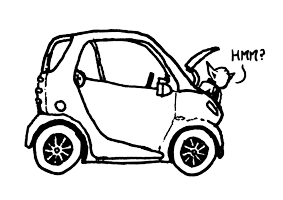
\includegraphics[scale=0.5, max width=0.8\textwidth]{imgs/a/3/06.png}
\caption{yoda in the engine block of a Smart Car}
\end{figure}

{At current electricity prices, Yoda would be worth about\$2/hour.}

{But telekinesis is just one type of Force power. What about that lightning the Emperor used to zap Luke? The physical nature of it is never made clear, but Tesla coils that produce \href{http://www.youtube.com/watch?v=uNJjnz-GdlE}{similar displays} draw something like \href{http://www.goodchildengineering.net/tesla-coils/drsstc-5-10kw-monster}{10 kilowatts} —which would put the Emperor roughly on par with Yoda. (Those Tesla coils use lots of very short pulses. If the Emperor is sustaining a continuous arc, as in an arc welder, the power could easily be in the megawatts.)}

{What about Luke? I examined the scene where he used his nascent Force powers to yank his lightsaber out of the snow. The numbers are harder to estimate here, but I went through frame-by-frame and came up with an estimate of 400 watts for his peak output. This is a fraction of Yoda's 19kW, and was sustained for only a fraction of a second.}

{So Yoda sounds like our best bet as an energy source. But with world electricity consumption pushing 2 terawatts, it would take a hundred million Yodas to meet our demands. All things considered, switching to Yoda Power probably isn’t worth the trouble—though it would \emph{definitely} be green.}

\begin{figure}[!htbp]
\centering

\includegraphics[scale=0.5, max width=0.8\textwidth]{imgs/a/3/yoda_07.png}
\caption{Yoda controlling and listening to an mp3 player with the force}
\end{figure}

{
\chapter{A Mole of Moles}
\phantomsection
%\addcontentsline{toc}{chapter}{A Mole of Moles}
%\addcontentsline{toc}{chapter}{A Mole of Moles}
}
\question{What would happen if you were to gather a mole (unit of measurement) of moles (the small furry critter) in one place?}

\hfill\attribute{—Sean Rice}

{Things get a bit gruesome.}

{First, some definitions. A mole is a unit. It’s not a typical unit, though. It’s really just a number—like “dozen” or “billion.” If you have a mole of something, it means you have 602,214,129,000,000,000,000,000 of them (usually written\( 6.022\times10^{23}\)). It’s such a big number because it’s used for counting numbers of molecules, which there are a lot of.}

\begin{figure}[!htbp]
\centering

\includegraphics[scale=0.5, max width=0.8\textwidth]{imgs/a/4/moles_too_many.png}
\caption{a figure with a hand overflowing with molecules}
\end{figure}

{"One mole" is close to the number of atoms in a gram of hydrogen. It’s also, by chance, a decent ballpark guess for the number of grains of sand on Earth.}

{A mole is also a type of burrowing mammal. There are a handful of types of moles, and some of them are \href{http://en.wikipedia.org/wiki/File:Condylura.jpg}{truly horrifying}.}

\begin{figure}[!htbp]
\centering

\includegraphics[scale=0.5, max width=0.8\textwidth]{imgs/a/4/moles_star_nosed.png}
\caption{a figure searching for, finding, and being scarred by a truly horrifying star-nosed mole on wikipedia}
\end{figure}

{So what would a mole of moles—602,214,129,000,000,000,000,000 animals—look like?}

{First, let’s start with wild ballpark approximations. This is an example of what might go through my head before I even pick up a calculator, when I’m just trying to get a sense of the quantities - the kind of calculation where 10, 1, and 0.1 are all close enough that we can consider them equal:}

{I can pick up a mole (animal) and throw it.[{citation needed} ]Anything I can throw weighs one pound. One pound is one kilogram. The number 602,214,129,000,000,000,000,000 looks about twice as long as a trillion, which means it’s about a trillion trillion. I happen to remember that a trillion trillion kilograms is how much a planet weighs.}

\begin{figure}[!htbp]
\centering

\includegraphics[scale=0.5, max width=0.8\textwidth]{imgs/a/4/moles_number_length.png}
\caption{illustration showing that a trillion is visually approximately one half of one mole}
\end{figure}

{… if anyone asks, I didnottell you it was ok to do math like this.}

{That’s enough to tell us that we’re talking about pile of moles on the scale of planets. It’s a pretty rough estimate, though, since it could be off by a factor of thousands in either direction.}

{Let’s get some better numbers.}

{An eastern mole ( \emph{Scalopus aquaticus}) weighs about 75 grams, which means a mole of moles weighs}

{\[ (6.022\times10^{23})\times75\mathrm{g}\approx4.52\times10^{22}\mathrm{kg}\]}

{That’s a little over half the mass of our moon.}

{Mammals are largely water. A kilogram of water takes up a liter of volume, so if the moles weigh\( 4.52\times10^{22}\) kilograms, they take up about\( 4.52\times10^{22}\) liters of volume. You might notice that we’re ignoring the pockets of space between the moles. In a moment, you’ll see why.}

{The cube root of\( 4.52\times10^{22}\) liters is 3,562 kilometers, which means we’re talking about a sphere with a radius of 2,210 kilometers, or a cube 2,213 miles on each edge. (That’s a neat coincidence I’ve never noticed before—a cubic mile happens to be almost exactly\(\frac{4}{3}\pi\) cubic kilometers, so a sphere with a radius of X kilometers has the same volume as a cube that’s X miles on each side.)}

{If these moles were released onto the Earth’s surface, they’d fill it up to 80 kilometers deep—just about to the (former) edge of space:}

\begin{figure}[!htbp]
\centering

\includegraphics[scale=0.5, max width=0.8\textwidth]{imgs/a/4/moles_layers.png}
\caption{cross section of the earth's surface with 80km of moles between the crust and displaced air before space}
\end{figure}

{This smothering ocean of high-pressure meat would wipe out most life on the planet, which could—to reddit’s horror—threaten the integrity of the DNS system. So doing this on Earth is definitely not an option.}

{Instead, let’s gather the moles in interplanetary space. Gravitational attraction would pull them into a sphere. Meat doesn’t compress very well, so it would only undergo a little bit of gravitational contraction, and we’d end up with a mole planet a bit larger than the moon.}

\begin{figure}[!htbp]
\centering

\includegraphics[scale=0.5, max width=0.8\textwidth]{imgs/a/4/moles_scale.png}
\caption{circles showing that a mole of moles makes a sphere slightly larger than our moon}
\end{figure}

{The moles would have a surface gravity about one-sixteenth as strong as Earth’s—similar to that of Pluto. The planet would start off uniformly lukewarm—probably a bit over room temperature—and the gravitational contraction would heat the deep interior by a handful of degrees.}

{But this is where it gets weird.}

{The mole planet is now a giant sphere of meat. It has a lot of latent energy (there are enough calories in the mole planet to support the Earth’s current population for 30 billion years). Normally, when organic matter decomposes, it releases much of that energy as heat. But throughout the majority of the planet’s interior, the pressure is over a hundred megapascals, which is enough to kill all bacteria and sterilize the mole remains—leaving no microorganisms to break down the mole tissues.}

{Closer to the surface, where the pressure is lower, there’s another obstacle to decomposition—the interior of a mole planet is low in oxygen. Without oxygen, the usual decomposition doesn’t happen, and the only bacteria that can break down the moles are those which don’t require oxygen. While inefficient, this anaerobic decomposition can unlock quite a bit of heat. If continued unchecked, it would heat the planet to a boil.}

{But the decomposition is self-limiting. Few bacteria can survive at temperatures above about 60 °C, so as the temperature goes up, the bacteria die off, and the decomposition slows. Throughout the planet, the mole bodies gradually break down into kerogen, a mush of organic matter which would—if the planet were hotter—eventually form oil.}

{The outer surface of the planet radiates heat into space and freezes. Because the moles form a literal fur coat, when frozen it insulates the interior of the planet and slows the loss of heat to space. However, the flow of heat in the liquid interior is dominated by convection. Plumes of hot meat and bubbles of trapped gases like methane—along with the air from the lungs of the deceased moles—periodically rise through the mole crust and erupt volcanically from the surface, a geyser of death blasting mole bodies free of the planet.}

{Eventually, after centuries or millennia of turmoil, the planet calms and cools enough that it begins to freeze all the way through. The deep interior is under such high pressure that as it cools, the water crystallizes out into \href{http://en.wikipedia.org/wiki/Ice\#Phases}{exotic forms of ice} such as ice III and ice V, and eventually ice II and ice IX (\href{http://en.wikipedia.org/wiki/Ice-nine}{no relation}).}

{All told, this is a pretty bleak picture. Let’s try an alternate approach.}

{I don’t have any reliable numbers for global mole population (or small mammal biomass in general), but we’ll take a shot in the dark and estimate that there are at least a few dozen mice, rats, voles, and other small mammals for every human.}

{There might be \href{http://blogs.discovermagazine.com/badastronomy/2010/10/29/how-many-habitable-planets-are-there-in-the-galaxy/}{a billion habitable planets} in our galaxy. If we colonized them, we’d certainly bring mice and rats with us. If just one in a hundred were populated with small mammals in numbers similar to Earth’s, after a few million years—not long, in evolutionary time—the total number which have ever lived would surpass Avogadro’s number.}

{If you want a mole of moles, build a spaceship.}

\begin{figure}[!htbp]
\centering

\includegraphics[scale=0.5, max width=0.8\textwidth]{imgs/a/4/moles_rocket.png}
\caption{a figure on a rocket with some small mammals}
\end{figure}

{
\chapter{Robot Apocalypse}
\phantomsection
%\addcontentsline{toc}{chapter}{Robot Apocalypse}
%\addcontentsline{toc}{chapter}{Robot Apocalypse}
}
\question{What if there was a robot apocalypse? How long would humanity last?}

\hfill\attribute{—Rob Lombino}

{Before I answer this question, let me give you a little background on where I’m coming from.}

{I’m by no means an expert, but I have some experience with robotics. My first job out of college was working on robots at NASA, and my undergraduate degree project was on robotic navigation. I spent my teenage years participating in \href{http://www.usfirst.org/}{FIRST Robotics}, programming software bots to fight in \href{http://en.wikipedia.org/wiki/RoboWar} {virtual tournaments}, and working on homemade underwater ROVs. And I've watched plenty of \emph{Robot Wars}, \emph{BattleBots}, and \emph{Killer Robots Robogames}.}

{If all that experience has taught me anything, it’s that the robot revolution would end quickly, because the robots would all break down or get stuck against walls. Robots never, ever work right.}

{What people don't appreciate, when they picture Terminator-style automatons striding triumphantly across a mountain of human skulls, is how hard it is to keep your footing on something as unstable as a mountain of human skulls. Most humans probably couldn't manage it, and they've had a lifetime of practice at walking without falling over.}

{Of course, our technology is constantly improving. But we have a long way to go. Instead of the typical futuristic robot apocalypse scenario, let's suppose that our current machines turned against us. We won’t assume any technological advances—just that all our current machines were reprogrammed to blindly attack us using existing technology.}

{Here are a few snapshots of what an \emph{actual} robot apocalypse might look like:}

{In labs everywhere, experimental robots would leap up from lab benches in a murderous rage, locate the door, and—with a tremendous crash—plow into it and fall over.}

\begin{figure}[!htbp]
\centering

\includegraphics[scale=0.5, max width=0.8\textwidth]{imgs/a/5/robot_apocalypse_door.png}
\caption{robots accelerating into a closed door with a comics style 'wham!' in a starburst}
\end{figure}

{Those robots lucky enough to have limbs that can operate a doorknob, or to have the door left open for them, would have to contend with deceptively tricky rubber thresholds before they could get into the hallway.}

\begin{figure}[!htbp]
\centering

\includegraphics[scale=0.5, max width=0.8\textwidth]{imgs/a/5/robot_apocalypse_threshold.png}
\caption{robot getting stuck in a doorway}
\end{figure}

{Hours later, most of them would be found in nearby bathrooms, trying desperately to exterminate what they have identified as a human overlord but is actually a paper towel dispenser.}

\begin{figure}[!htbp]
\centering

\includegraphics[scale=0.5, max width=0.8\textwidth]{imgs/a/5/robot_apocalypse_comparison.png}
\caption{two panels, one labeled unlikely with the terminator as a humanoid robot and one labled likely with the terminator as a small robot hitting sarah connor's leg}
\end{figure}

{But robotics labs are only a small part of the revolution. There are computers all around us. What about the machines closest to us? Could our cell phones turn against us?}

{Yes, but their options for attacking us are limited. They could run up huge credit card bills, but the computers would control our financial system anyway—and frankly, judging from the headlines lately, that might be more of a liability than an asset.}

{So the phones would be reduced to attacking us directly. It would start with annoying ringtones and piercing noises. Then kitchen tables around the country would rattle as the phones all turned on their ‘vibrate’ functions, hoping to work their way to the edges and fall on unprotected toes.}

\begin{figure}[!htbp]
\centering

\includegraphics[scale=0.5, max width=0.8\textwidth]{imgs/a/5/robot_apocalypse_phone.png}
\caption{a phone vibrating menacingly off of a table with a figure standing by}
\end{figure}

{All modern cars contain computers, so they’d join the revolution. But most of them are parked. Even if they were able to get in gear, without a human at the wheel, few of them have any way to tell where they’re going. They might \emph{want} to run us down, \href{http://en.wikipedia.org/wiki/The\_Honking}{Futurama-style}, but they’d have no way to find us. They’d have to accelerate blindly and hope they hit something important—and there are a lot more trees and telephone poles in the world than human targets.}

{The cars currently on the road would be more dangerous, but mainly to their occupants. Which raises a question—how many people are driving at any given time? Americans drive \href{http://www.fhwa.dot.gov/policyinformation/travel\_monitoring/12maytvt/page2.cfm}{three trillion miles} each year, and moving cars average around \href{http://www.dieseltruckresource.com/dev/archive/average-mph-over-life-t118709.html} {30 miles per hour}, which means that there are normally an average of about ten million cars on US roads:}

{\[\frac{3\text{ trillion}\frac{\mathrm{miles}}{\mathrm{year}}}{30\frac{\mathrm{mph}}{\text{car}}}\approx10\text{ million cars}\]}

{So those ten million drivers (and \href{http://www.mtc.ca.gov/maps\_and\_data/datamart/forecast/ass98\_tab8.htm}{a few million passengers}) would definitely be in peril. But they’d have some options to fight back. While the cars might be able to control the throttle and disable the power steering, the driver would still control the steering wheel, which has direct mechanical linkage to the wheels. The driver could also pull the parking brake, although I know from experience how easily a car can drive with one of those on. Some cars might try to disable the drivers by deploying the air bags, then roll over or drive into things. In the end, our cars would probably take a heavy toll, but not a decisive one.}

{Our biggest robots are the ones found in factories-but those are bolted to the floor. While they're dangerous if you happen to within arm’s reach, what would they do once everyone fled? All they can really do is assemble things. Half of them would probably try to attack us by \emph{not} assembling things, and half by assembling \emph{more} things. The end result would be no real change.}

{Battlebots, on the face of it, seem like they’d be among the most dangerous robo-soldiers. But it’s hard to feel threatened by something that you can evade by sitting on the kitchen counter and destroy by letting the sink overflow.}

\begin{figure}[!htbp]
\centering

\includegraphics[scale=0.5, max width=0.8\textwidth]{imgs/a/5/robot_apocalypse_battlebot.png}
\caption{a battlebot being thrwarted by a figure sitting on a kitchen counter running water and shorting it out}
\end{figure}

{Military bomb-disposal and riot-control robots would be a little more menacing, but there are only so many of them in the world, and most of them are likely kept in boxes or storage lockers. Any stray machine-gun-armed prototype military robots that did get loose could be subdued in seconds by a couple of firefighters.}

{Military drones probably \href{http://xkcd.com/652/}{fit the Terminator description} more closely than anything else around, and there’s no getting around the fact that they’d be pretty dangerous. However, they’d quickly run out of both fuel and missiles. Furthermore, they’re not all going to be in the air at any given time. Much of our fleet would be left helplessly bumping against hangar doors like Roombas stuck in a closet.}

{But this brings us to the big one: our nuclear arsenal.}

{In theory, \href{http://articles.chicagotribune.com/1999-11-11/news/9911110121\_1\_nuclear-weapons-y2k-launch}{human intervention is required} to launch nuclear weapons. In practice, while there’s no Skynet-style system issuing orders, there are certainly computers involved at every level of the decision, both communicating and displaying information. In our scenario, all of them would be compromised. Even if the actual \href{http://en.wikipedia.org/wiki/Two-man\_rule\#Nuclear\_weapons}{turning of the keys} requires people, the computers talking to all those people can lie. Some people might \href{http://en.wikipedia.org/wiki/Vasiliy\_Arkhipov\#Cuban\_Missile\_Crisis}{ignore} the \href{http://en.wikipedia.org/wiki/Stanislav\_Petrov} {order}, but some certainly wouldn’t.}

{But there’s a version of this story where there’s still hope for us.}

{We’ve been assuming so far that the computers care only about destroying us. But if this is a \emph{revolution} —if they’re trying to usurp us—then they need to survive. And nuclear weapons could be more dangerous to the robots than to us.}

{In addition to the blast and fallout, nuclear explosions generate powerful electromagnetic pulses. These EMPs overload and destroy delicate electronic circuits. This effect is fairly short-range under normal circumstances, but people and computers tend to be found in the same places. They can’t hit us without hitting themselves.}

{And nuclear weapons could actually give us an edge. If we managed to set any of them off in the upper atmosphere, the EMP effect would be \href{http://en.wikipedia.org/wiki/The\_K\_Project}{much more powerful}. Even if their attack doomed our civilization, a few lucky strikes on our part-or screwups on theirs-could wipe them out almost completely.}

{Which means the most important question of all is: \href{http://www.youtube.com/watch?v=NHWjlCaIrQo}{Have they ever played Tic-Tac-Toe?}}

\begin{figure}[!htbp]
\centering

\includegraphics[scale=0.5, max width=0.8\textwidth]{imgs/a/5/robot_apocalypse_end.png}
\caption{a figure asking a robot to be friends. the robot says 'frien- process 'negotiate with humans' has encountered an error and was shut down'. the figure says '...close enough!'}
\end{figure}

{
\chapter{Glass Half Empty}
\phantomsection
%\addcontentsline{toc}{chapter}{Glass Half Empty}
%\addcontentsline{toc}{chapter}{Glass Half Empty}
}
\question{What if a glass of water was, all of a sudden, literally half empty?}

\hfill\attribute{—Vittorio Iacovella}

{The pessimist is probably more right about how it turns out than the optimist.}

{When people say “glass half empty”, they usually mean something like a glass containing equal parts water and air:}

\begin{figure}[!htbp]
\centering

\includegraphics[scale=0.5, max width=0.8\textwidth]{imgs/a/6/glass_people.png}
\caption{an optimist and pessimist sitting at a table with a half-full - or half-empty glass between them. the optimist's thought bubble reads 'ooh-water! i bet we'll get to drink it!' while the pessimist's thought bubble reads 'drinking fluids postpones death but doesn't avert it.'}
\end{figure}

{Traditionally, the optimist sees the glass as half full while the pessimist sees it as half empty. This has spawned a zillion joke variants—e.g., the engineer sees a glass that’s twice as big as it needs to be, the surrealist sees a giraffe eating a necktie, etc.}

{But what if the empty half of the glass were \emph{actually} empty—a vacuum? (Even a vacuum arguably isn’t truly empty, but that’s a question for quantum semantics.)}

{The vacuum would definitely not last long. But exactly what happens depends on a key question that nobody usually bothers to ask: \emph{Which} half is empty?}

{For our scenario, we’ll imagine three different half-empty glasses, and follow what happens to them microsecond by microsecond.}

\begin{figure}[!htbp]
\centering

\includegraphics[scale=0.5, max width=0.8\textwidth]{imgs/a/6/glass_three.png}
\caption{three half-empty glasses of water}
\end{figure}

{In the middle is the traditional air/water glass. On the right is a glass like the traditional one, except the air is replaced by a vacuum. The glass on the left is half full of water and half empty—but it’s the \emph{bottom} half that’s empty.}

{We’ll imagine the vacuums appear at time t=0.}

\begin{figure}[!htbp]
\centering

\includegraphics[scale=0.5, max width=0.8\textwidth]{imgs/a/6/glass_0s.png}
\caption{three half-empty glasses of water at t=0}
\end{figure}

{For the first handful of microseconds, nothing happens. On this timescale, even the air molecules are nearly stationary.}

\begin{figure}[!htbp]
\centering

\includegraphics[scale=0.5, max width=0.8\textwidth]{imgs/a/6/glass_50ns.png}
\caption{three half-empty glasses of water at t=50us}
\end{figure}

{For the most part, air molecules jiggle around at speeds of a few hundred meters per second. But at any given time, some happen to be moving faster than others. The fastest few are moving at over 1000 meters per second. These are the first to drift into the vacuum in the glass on the right.}

{The vacuum on the left is surrounded by barriers, so air molecules can’t easily get in. The water, being a liquid, doesn’t expand to fill the vacuum in the same way air does. However, in the vacuum of the glasses, it does start to boil, slowly shedding water vapor into the empty space.}

\begin{figure}[!htbp]
\centering

\includegraphics[scale=0.5, max width=0.8\textwidth]{imgs/a/6/glass_150ns.png}
\caption{three half-empty glasses at t=150us}
\end{figure}

{While the water on the surface in both glasses starts to boil away, in the glass on the right, the air rushing in stops it before it really gets going. The glass on the left continues to fill with a very faint mist of water vapor.}

\begin{figure}[!htbp]
\centering

\includegraphics[scale=0.5, max width=0.8\textwidth]{imgs/a/6/glass_400ns.png}
\caption{three half-empthy glasses at t=400us}
\end{figure}

{After a few hundred microseconds, the air rushing into the glass on the right fills the vacuum completely and rams into the surface of the water, sending a pressure wave through the liquid. The sides of the glass bulge slightly, but they contain the pressure and do not break. A shockwave reverberates through the water and back into the air, joining the turbulence already there.}

\begin{figure}[!htbp]
\centering

\includegraphics[scale=0.5, max width=0.8\textwidth]{imgs/a/6/glass_1ms.png}
\caption{three half-empty glasses at t=1ms}
\end{figure}

{The shockwave from the vacuum collapse takes about a millisecond to spread out through the other two glasses. The glass and water both flex slightly as the wave passes through them. In a few more milliseconds, it reaches the humans’ ears as a loud bang.}

\begin{figure}[!htbp]
\centering

\includegraphics[scale=0.5, max width=0.8\textwidth]{imgs/a/6/glass_2ms.png}
\caption{three half-empty glasses at t=2ms}
\end{figure}

{Around this time, the glass on the left starts to visibly lift into the air.}

{The air pressure is trying to squeeze the glass and water together. This is the force we think of as suction. The vacuum on the right didn’t last long enough for the suction to lift the glass, but since air can’t get into the vacuum on the left, the glass and the water begin to slide toward each other.}

\begin{figure}[!htbp]
\centering

\includegraphics[scale=0.5, max width=0.8\textwidth]{imgs/a/6/glass_5ms.png}
\caption{three half-empty glasses at t=5ms}
\end{figure}

{The boiling water has filled the vacuum with a very small amount of water vapor. As the space gets smaller, the buildup of water vapor slowly increases the pressure on the water’s surface. Eventually, this will slow the boiling, just like higher air pressure would.}

\begin{figure}[!htbp]
\centering

\includegraphics[scale=0.5, max width=0.8\textwidth]{imgs/a/6/glass_8ms.png}
\caption{three half-empty glasses at t=8ms}
\end{figure}

{However, the glass and water are now moving too fast for the vapor buildup to matter. Less than ten milliseconds after the clock started, they’re flying toward each other at several meters per second. Without a cushion of air between them—only a few wisps of vapor—the water smacks into the bottom of the glass like a hammer.}

\begin{figure}[!htbp]
\centering

\includegraphics[scale=0.5, max width=0.8\textwidth]{imgs/a/6/glass_10ms.png}
\caption{three half-empty glasses at t=10ms}
\end{figure}

{Water is very nearly incompressible, so the impact isn’t spread out—it comes as a single sharp shock. The momentary force on the glass is immense, and it breaks.}

{This “water hammer” effect (which is also responsible for the “clunk” you sometimes hear in old plumbing when you turn off the faucet) can be seen in the well-known party trick (recorded on Mythbusters, analyzed in physics classes, and demonstrated in countless student dorms) of \href{http://www.youtube.com/watch?v=77gWkl0ZUC8}{smacking the top of a glass bottle to blow out the bottom.}}

{When the bottle is struck, it’s pushed suddenly downward. The liquid inside doesn’t respond to the suction (air pressure) right away—much like in our scenario—and a gap briefly opens up. It’s a small vacuum—a few fractions of an inch thick—but when it closes, the shock breaks the bottom of the bottle.}

{In our situation, the forces would be more than enough to destroy even the heaviest drinking glasses.}

\begin{figure}[!htbp]
\centering

\includegraphics[scale=0.5, max width=0.8\textwidth]{imgs/a/6/glass_20ms.png}
\caption{three half-empty glasses at t=20ms}
\end{figure}

{The bottom is carried downward by the water and thunks against the table. The water splashes around it, spraying droplets and glass shards in all directions.}

{Meanwhile, the detached upper portion of the glass continues to rise.}

\begin{figure}[!htbp]
\centering

\includegraphics[scale=0.5, max width=0.8\textwidth]{imgs/a/6/glass_500ms.png}
\caption{three half-empty glasses at t=500ms zoomed out to the table with the optimist (thinking 'Coool!') and the pessimist (thinking 'uh oh.')}
\end{figure}

{After half a second, the observers, hearing a pop, have begun to flinch. Their heads lift involuntarily to follow the rising movement of the glass.}

\begin{figure}[!htbp]
\centering

\includegraphics[scale=0.5, max width=0.8\textwidth]{imgs/a/6/glass_1s.png}
\caption{two half-empty glasses on the table at t=1s, the third glass breaking into fragments }
\end{figure}

{The glass has just enough speed to bang against the ceiling, breaking into fragments…}

\begin{figure}[!htbp]
\centering

\includegraphics[scale=0.5, max width=0.8\textwidth]{imgs/a/6/glass_1_5s.png}
\caption{two half-empty glasses on the table at t=1.5s, the third glass now a mass of fragments raining down from the ceiling.}
\end{figure}

{… which, their momentum now spent, return to the table.}

\begin{figure}[!htbp]
\centering

\includegraphics[scale=0.5, max width=0.8\textwidth]{imgs/a/6/glass_10s.png}
\caption{two half-empty glasses on the table at t=10s, the third now embedded in the faces of the optimist ('Hey, free glass!') and pessimist ('Aaaaaaa')}
\end{figure}

{The lesson: If the optimist says the glass is half full, and the pessimist says the glass is half empty, the physicist ducks.}

\begin{figure}[!htbp]
\centering

\includegraphics[scale=0.5, max width=0.8\textwidth]{imgs/a/6/glass_end.png}
\caption{the glass-studded optimisit pours water from one of the remaining half-empty glasses into the other. the pessimist's chair is empty.}
\end{figure}

{
\chapter{Everybody Out}
\phantomsection
%\addcontentsline{toc}{chapter}{Everybody Out}
%\addcontentsline{toc}{chapter}{Everybody Out}
}
\question{Is there enough energy to move the entire current human population off-planet?}

\hfill\attribute{—Adam}

{There are a bunch of science fiction movies where, because of pollution, overpopulation, or nuclear war, humanity abandons Earth.}

{But lifting people into space is hard. Barring a massive reduction in the population, is launching the whole human race into space physically possible? Let’s not even worry about where we’re headed—we’ll assume we don’t have to find a new home, but we can’t stay here.}

\begin{figure}[!htbp]
\centering

\includegraphics[scale=0.5, max width=0.8\textwidth]{imgs/a/7/everybody_out_plan.png}
\caption{people being cut off and sent floating into space in bubble}
\end{figure}

{To figure out if this is plausible, we can start with an absolute baseline energy requirement: four gigajoules per person. No matter how we do it, whether we use rockets or a cannon or a space elevator, moving a 65-kilogram person—or 65 kilograms of anything—out of the Earth’s gravity well requires at least this much energy.}

{\[\text{Gravitational potential energy} =\frac{1}{2}\times 65\mathrm{kg}\times\text{(Earth escape velocity)}^{2}\]}

{The energy required to lift something away from the Earth is equal to its kinetic energy if it were moving at Earth’s escape velocity.}

{How much is four gigajoules? It’s about a megawatt-hour, which is what a typical US household consumes in electricity in a month or two. It’s the amount of stored energy in a cargo van full of AA batteries or 90 kg of gasoline.}

\begin{figure}[!htbp]
\centering

\includegraphics[scale=0.5, max width=0.8\textwidth]{imgs/a/7/everybody_out_cargo_van.png}
\caption{an avalanche of batteries falling out of the open back of a cargo van}
\end{figure}

{Four gigajoules times seven billion people gives us\(2.8\times 10^{18}\) joules, or 8 petawatt-hours. This is about five percent of the world’s annual energy consumption. A lot, but not impossible.}

{But this is just a minimum. In practice, everything depends on our means of transportation. If we’re using rockets, it’s going to take a lot more. This is because of a fundamental problem with rockets: they have to lift their own fuel.}

{Let’s return for a moment to those 90 kilograms of gasoline (about 30 gallons), because they help illustrate a central problem in space travel.}

{If we want to launch a 65-kilogram spaceship, we need to burn around 90 kilograms of fuel. (Gasoline has an energy per pound comparable to that of rocket fuel, so we’ll stick with that example). We load that fuel on board—and now our spaceship weighs 155 kilograms. A 155-kilogram spaceship requires 215 kilograms of fuel, so we load another 125 kilograms on board...}

{Fortunately, we’re saved from an infinite loop—where we add 1.3 kilograms for every 1 kilogram we add—by the fact that we don’t have to carry that fuel all the way up. We burn it as we go, so we get lighter and lighter, which means we need less and less fuel. But we do have to lift the fuel partway. The formula for how much propellant we need to burn to get moving at a given speed is given by the Tsiolkovsky Rocket equation:}

{\[\Delta v = v_\text{exhaust}\ln\frac {m_\text{start}} {m_\text{end}}\]}

{\(m_\text{start}\) and\(m_\text{end}\) are the total mass of the ship+fuel before and after the burn, and\(v_\text{exhaust}\) is the “exhaust velocity” of the fuel, a number that’s between 2.5-4.5 km/s for rocket fuels.}

{What’s important is the ratio between\(\Delta v\) and\(v_\text{exhaust}\) — the speed we want to be going compared to the speed that the propellant exits our rocket. The kilograms of fuel needed per kilogram of ship is e to the power of this number, which gets big very fast. For leaving Earth, we need a\(\Delta v\) of upwards of 13 km/s, and\(v_\text{exhaust}\) isn’t much higher than 4.5 km/s, which gives a fuel-to-ship ratio of at least\(\text{e}^{\frac{13}{4.5}}\approx 20\).}

{The upshot is that to overcome Earth’s gravity using traditional rocket fuels, a one-ton craft needs 20 to 50 tons of fuel. Launching all of humanity (total weight: around 400 million tons) would therefore take tens of trillions of tons of fuel. That’s a lot; if we were using hydrocarbon-based fuels, it would represent a decent chunk of the world’s remaining oil reserves. And that’s not even worrying about the weight of the ship itself, food, water, or our pets (there are probably around a million tons of pet dog in the US alone). We’d also need fuel to produce all these ships, to transport people to the launch sites, and so forth. It’s not necessarily completely impossible, but it’s certainly outside the realm of plausibility.}

{But rockets aren’t our only option. As crazy as it sounds, we might be better off trying to (1) literally climb into space on a rope, or (2) blow ourselves off the planet with nuclear weapons. These are actually serious—if audacious—ideas for launch systems, both of which have been bouncing around since the start of the Space Age.}

\begin{figure}[!htbp]
\centering

\includegraphics[scale=0.5, max width=0.8\textwidth]{imgs/a/7/everybody_out_crazy.png}
\caption{two figures climbing a rope off the earth and an exploded earth with a craft flying off of it}
\end{figure}

{The first approach is the “space elevator” concept, a favorite of science fiction authors. The idea is that we connect a tether to a satellite orbiting far enough out that the tether is held taut by centrifugal force. Then we can send climbers up the rope using ordinary electricity and motors, powered by solar power, nuclear generators, or whatever works best. The biggest engineering hurdle is that the tether would have to be several times stronger than anything we can currently build. There are hopes that carbon nanotube-based materials could provide the required strength—adding this to the long list of engineering problems which can be waved away by tacking on the prefix “nano-”.}

{The second approach is nuclear pulse propulsion, a surprisingly plausible method for getting huge amounts of material moving really fast. The basic idea is that you toss a nuclear bomb behind you and ride the shockwave. You’d think the spacecraft would be vaporized, but it turns out that if it has a well-designed shield, the blast flings away before it has a chance to disintegrate. If it could be made reliable enough, this system would in theory be capable of lifting entire city blocks into orbit, and could—potentially—accomplish our goal.}

{The engineering principles behind this were solid enough that in the 1960s, under the guidance of Freeman Dyson, the US government actually tried to build one of these spaceships. The story of that effort, dubbed Project Orion, is detailed in the excellent \href{http://www.amazon.com/Project-Orion-Story-Atomic-Spaceship/dp/0805059857}{book} of the same name by Freeman’s son George Dyson. Advocates for nuclear pulse propulsion are still disappointed that the project was cancelled before any prototypes were built. Others argue that when you think about what they were trying to do—put our entire nuclear arsenal in a box, hurl it high into the atmosphere, and nuke it repeatedly—it’s terrifying that it got as far as it did.}

{So the answer is that while sending one person into space is easy, getting all of us there would tax our resources to the limit and possibly destroy the planet. It’s a small step for a man, but a giant leap for mankind.}

{
\chapter{Everybody Jump}
\phantomsection
%\addcontentsline{toc}{chapter}{Everybody Jump}
%\addcontentsline{toc}{chapter}{Everybody Jump}
}
\question{What would happen if everyone on earth stood as close to each other as they could and jumped, everyone landing on the ground at the same instant?}

\hfill\attribute{—Thomas Bennett (and many others)}

{This is one of the most popular questions submitted to this blog. It’s been examined before, including by a \href{http://scienceblogs.com/dotphysics/2010/08/26/what-if-everyone-jumped/}{ScienceBlogs} post and a \href{http://www.straightdope.com/columns/read/142/if-all-chinese-jumped-at-once-would-cataclysm-result} {Straight Dope article}. They cover the kinematics pretty well. However, they don’t tell the whole story.}

{Let’s take a closer look.}

{At the start of the scenario, the entire Earth’s population has been magically transported together into one place.}

\begin{figure}[!htbp]
\centering

\includegraphics[scale=0.5, max width=0.8\textwidth]{imgs/a/8/everybody_jump_standing.png}
\caption{several stick figure characters standing around}
\end{figure}

{This crowd takes up an area the size of Rhode Island. But there’s no reason to use the vague phrase “an area the size of Rhode Island”. This is our scenario; we can be specific. They’re \emph{actually} in Rhode Island.}

\begin{figure}[!htbp]
\centering
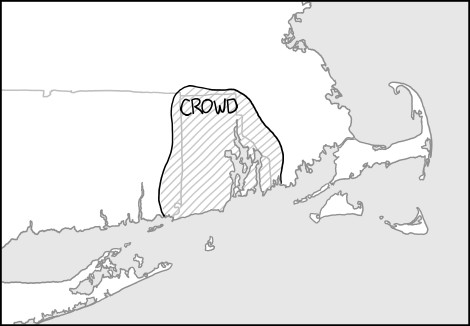
\includegraphics[scale=0.5, max width=0.8\textwidth]{imgs/a/8/everybody_jump_map1.png}
\caption{map showing Rhode Island and with a outlined section labeled 'crowd'}
\end{figure}

{At the stroke of noon, everyone jumps.}

\begin{figure}[!htbp]
\centering

\includegraphics[scale=0.5, max width=0.8\textwidth]{imgs/a/8/everybody_jump_jumping.png}
\caption{the stick figure characters, who had been standing, now jumping in a variety of poses}
\end{figure}

{As discussed elsewhere, it doesn’t really affect the planet. Earth outweighs us by a factor of over ten trillion. On average, we humans can vertically jump maybe half a meter on a good day. Even if the Earth were rigid and responded instantly, it would be pushed down by less than an atom’s width.}

{Next, everyone falls back to the ground.}

\begin{figure}[!htbp]
\centering

\includegraphics[scale=0.5, max width=0.8\textwidth]{imgs/a/8/everybody_jump_standing.png}
\caption{all the stick figure characters now standing again}
\end{figure}

{Technically, this delivers a lot of energy into the Earth, but it’s spread out over a large enough area that it doesn’t do much more than leave footprints in a lot of gardens. A slight pulse of pressure spreads through the North American continental crust and dissipates with little effect. The sound of all those feet hitting the ground creates a loud, drawn-out roar which lasts many seconds.}

{Eventually, the air grows quiet.}

{Seconds pass. Everyone looks around.}

\begin{figure}[!htbp]
\centering

\includegraphics[scale=0.5, max width=0.8\textwidth]{imgs/a/8/everybody_jump_talking1.png}
\caption{the stick figure characters standing around. one says 'why did we do that?', another says '...is this rhode island?}
\end{figure}

{There are a lot of uncomfortable glances. Someone coughs.}

\begin{figure}[!htbp]
\centering

\includegraphics[scale=0.5, max width=0.8\textwidth]{imgs/a/8/everybody_jump_talking2.png}
\caption{same standing stick figure characters. one says 'I should get back to Dublin', one says, in Hindi, 'Where's the airport?'}
\end{figure}

{A cell phone comes out of a pocket. Within seconds, the rest of the world’s five billion phones follow. All of them—even those compatible with the region’s towers—are displaying some version of “NO SIGNAL”. The cell networks have all collapsed under the unprecedented load.}

{Outside Rhode Island, abandoned machinery begins grinding to a halt.}

{The T. F. Green airport in Warwick, Rhode Island handles a few thousand passengers a day. Assuming they got things organized (including sending out scouting missions to retrieve fuel), they could run at 500\% capacity for years without making a dent in the crowd.}

\begin{figure}[!htbp]
\centering
\includegraphics[scale=0.5, max width=0.8\textwidth]{imgs/a/8/everybody_jump_map2.png}
\caption{the map of Rhode Island where the crowd was outlined with arrows signifying everyone trying to leave}
\end{figure}

{The addition of all the nearby airports doesn’t change the equation much. Nor does the region’s light rail system. Crowds climb on board container ships in the deepwater port of Providence, but stocking sufficient food and water for a long sea voyage proves a challenge.}

{Rhode Island’s half-million cars are commandeered. Moments later, I-95, I-195, and I-295 become the sites of the largest traffic jam in the history of the planet. Most of the cars are engulfed by the crowds, but a lucky few get out and begin wandering the abandoned road network.}

{Some make it past New York or Boston before running out of fuel. Since the electricity is probably not on at this point, rather than find a working gas pump, it’s easier to just abandon the car and steal the new one. Who can stop you? All the cops are in Rhode Island.}

{The edge of the crowd spreads outward into southern Massachusetts and Connecticut. Any two people who meet are unlikely to have a language in common, and almost nobody knows the area. The state becomes a patchwork chaos of coalescing and collapsing social hierarchies. Violence is common. Everybody is hungry and thirsty. Grocery stores are emptied. Fresh water is hard to come by and there’s no efficient system for distributing it.}

{Within weeks, Rhode Island is a graveyard of billions.}

{The survivors spread out across the face of the world and struggle to build a new civilization atop the pristine ruins of the old. Our species staggers on, but our population has been greatly reduced. Earth’s orbit is completely unaffected—it spins along exactly as it did before our species-wide jump.}

{But at least now we know.}

\begin{figure}[!htbp]
\centering
\includegraphics[scale=0.5, max width=0.8\textwidth]{imgs/a/8/everybody_jump_earth.png}
\caption{You did, this, Brandon.}
\end{figure}

{
\chapter{Soul Mates}
\phantomsection
%\addcontentsline{toc}{chapter}{Soul Mates}
%\addcontentsline{toc}{chapter}{Soul Mates}
}
\question{What if everyone actually had only one soul mate, a random person somewhere in the world?}

\hfill\attribute{—Benjamin Staffin}

{What a nightmare that would be.}

{There are a lot of problems with the concept of a single random soul mate. As Tim Minchin put it in his song \href{http://www.youtube.com/watch?v=Gaid72fqzNE}{If I Didn’t Have You:}}

{Your love is one in a million
You couldn’t buy it at any price.}

{But of the 9.999 hundred thousand other loves,
Statistically, some of them would be equally nice.}

{But what if we did have one randomly-assigned perfect soul mate, and we couldn’t be happy with anyone else? Would we find each other?}

{We’ll assume your soul mate is set at birth. You know nothing about who or where they are, but—as in the romantic cliché—you’ll recognize each other the moment your eyes meet.}

{Right away, this raises a few questions. For starters, is your soul mate even still alive? A hundred billion or so humans have ever lived, but only seven billion are alive now (which gives the human condition a 93\% mortality rate). If we’re all paired up at random, 90\% of our soul mates are long dead.}

\begin{figure}[!htbp]
\centering
\includegraphics[scale=0.5, max width=0.8\textwidth]{imgs/a/9/soulmates_died.png}
\caption{an assortment of stickfigure characters, dying in a range of dates, from 63,556 BCE to someone who is alive (but only until 2014)}
\end{figure}

{That sounds horrible. But wait, it gets worse: A simple argument shows we can’t just limit ourselves to past humans; we have to include an unknown number of future humans as well. See, if it’s possible for your soul mate to be in the distant past, then it \emph{also} has to be possible for soul mates to be in the distant future. After all, \emph{your} soul mate’s soul mate is.}

{So let’s assume your soul mate lives at the same time as you. Furthermore, to keep things from getting creepy, we’ll assume they’re within a few years of your age. (This is stricter than the \href{http://xkcd.com/314/}{standard age gap creepiness formula}, but if we assume a 30-year-old and a 40-year-old can be soul mates, then the creepiness rule is violated if they accidentally meet 15 years earlier.) With the same-age restriction, most of us have a pool of around half a billion potential matches.}

{But what about gender and sexual orientation? And culture? And language? We could keep using demographics to try to break things down further, but we’d be drifting away from the idea of a random soul mate. In our scenario, you don’t know anything about who your soul mate will be until you look into their eyes. Everybody has only one orientation—toward their soul mate.}

{The odds of running into your soul mate are incredibly small. The number of strangers we make eye contact with each day is hard to estimate. It can vary from almost none (shut-ins or people in small towns) to many thousands (a police officer in Times Square). Let’s suppose you lock eyes with an average of a few dozen new strangers each day. (I’m pretty introverted, so for me that’s definitely a generous estimate.) If 10\% of them are close to your age, that’s around 50,000 people in a lifetime. Given that you have 500,000,000 potential soul mates, it means you’ll only find true love in one lifetime out of ten thousand.}

\begin{figure}[!htbp]
\centering
\includegraphics[scale=0.5, max width=0.8\textwidth]{imgs/a/9/soulmates_10000.png}
\caption{a block of 10,000 blocks, showing one out of 10,000 finding their soul mate and the remaining being 'alone forever'}
\end{figure}

{But with the threat of dying alone looming so imminently, society could restructure to try to enable as much eye contact as possible. We could put together massive conveyer belts to move lines of people past each other …}

\begin{figure}[!htbp]
\centering
\includegraphics[scale=0.5, max width=0.8\textwidth]{imgs/a/9/soulmates_conveyor.png}
\caption{several stick figure characters on two conveyer belts going opposite directions, passing each other.}
\end{figure}

{... but if the eye contact effect works over webcams, we could just use a modified version of ChatRoulette.}

\begin{figure}[!htbp]
\centering
\includegraphics[scale=0.5, max width=0.8\textwidth]{imgs/a/9/soulmates_laptop.png}
\caption{two stick figure characters, one on a computer and one standing behind them. the standing behind them says '...yup, another butt.' and the one on the computer says 'but it could be my soul mate's butt!'}
\end{figure}

{If everyone used the system for eight hours a day, seven days a week, and if it takes you a couple seconds to decide if someone’s your soul mate, this system could—in theory—match everyone up with their soul mates in a few decades. (I modeled a few simple systems to estimate how quickly people would pair off and drop out of the singles pool. If you want to try to work through the math for a particular setup, you might start by looking at \href{http://en.wikipedia.org/wiki/Derangement}{derangement problems}.)}

{In the real world, many people have trouble finding any time at all for romance—few could devote two decades to it. So maybe only rich kids would be able to afford to sit around on SoulMateRoulette. Unfortunately for the proverbial 1\%, most of their soul mates are to be found in the other 99\%. If only 1\% of people use the service, then 1\% of that 1\% would find their match through this system—one in ten thousand.}

{The other 99\% of the 1\% (“We are the zero point nine nine percent!”) would have an incentive to get more people into the system. They might sponsor projects akin to One Laptop Per Child (but with a sleazier vibe). Careers like “cashier” and “police officer in Times Square” would become high-status prizes because of the eye contact potential. People would flock to cities and public gathering places to find love—just as they do now.}

{But even if a bunch of us spent years on SoulMateRoulette, another bunch of us managed to hold jobs that offered constant eye contact with strangers, and the rest of us just hoped for luck, only a small minority of us would ever find true love. The rest of us would be out of luck.}

{Given all the stress and pressure, some people would fake it. They’d want to join the club, so they’d get together with another lonely person and stage a fake soul mate encounter. They’d marry, hide their relationship problems, and struggle to present a happy face to their friends and family. (Of course, this never happens in our world.)}

{All in all, the world of random soul mates is an even lonelier one than ours. I prefer Tim Minchin’s take on things:}

{With all my heart and all my mind I know one thing is true:
I have just one life and just one love and, my love, that love is you.}

{And if it wasn't for you, baby,
I really think that I would
have somebody else.}

{
\chapter{Cassini}
\phantomsection
%\addcontentsline{toc}{chapter}{Cassini}
%\addcontentsline{toc}{chapter}{Cassini}
}
\question{What would the world be like if the land masses were spread out the same way as now - only rotated by an angle of 90 degrees?}

\hfill\attribute{—Socke}

{It would profoundly alter our biosphere in general and public radio in particular.}

{Socke asks what would happen if the Earth’s surface were slid around by 90 degrees, putting our current North and South Poles on the equator. We’re not changing the tilt of the Earth’s axis; we’re just imagining that the surface were arranged differently.}

\begin{figure}[!htbp]
\centering
\includegraphics[scale=0.5, max width=0.8\textwidth]{imgs/a/10/cassini_flip.png}
\caption{a diagram showing the new location of the equator and the poles}
\end{figure}

{We’ll pick the Greenwich meridian for our new equator, putting the new North and South poles in the Indian ocean (0N, 90E) and off the coast of Ecuador (0N, 90W). India, Indonesia, and Ecuador would become polar, while Europe, Antarctica, and Alaska would become tropical.}

{Where would the deserts and forests be? What areas would get better or worse?}

{This stuff is complicated. In a moment, we'll start using wild speculation to reshape the face of the planet. But first, a brief story to illustrate just how mind-bogglingly complicated this stuff is:}

{In Chad, on the southern outskirts of the Sahara, there’s valley called the Bodélé Depression. It was once a lakebed, and the dry dust in the valley floor is full of nutrient-rich matter from the microorganisms that lived there.}

{From October to March, winds coming in from the east are pinched between two mountain ranges. When the surface winds climb over 20 mph, they start picking up dust from the valley. This dust is blown westward, all the way across Africa, and out over the Atlantic.}

{That dirt—from one small valley in Chad— \href{http://iopscience.iop.org/1748-9326/1/1/014005}{supplies over 50\% of the nutrient-rich dust that helps fertilize the Amazon rainforest}.}

{At least, according to that one study. But if it's right, it wouldn’t be a crazy anomaly. This kind of complexity is found \emph{everywhere}. The basic building blocks of our world are \emph{crazy}.}

{This is why we can be so certain about large-scale patterns like global warming, where we understand the overall physics pretty well—energy comes in, less energy goes out, so the average temperature rises—but have a harder time predicting how it will affect any particular place or specific species.}

{So even if I were a climate expert—which I’m definitely not—there’d be no way to answer this question with certainty. There are just too many variables. Instead, think of what follows as a rough sketch of some of the things this alternate Earth could contain.}

{To start, here’s a map of our reshuffled world:}

\begin{figure}[!htbp]
\centering
\includegraphics[scale=0.5, max width=0.8\textwidth]{imgs/a/10/cassini_blank.png}
\caption{a map of the reshuffled earth, with asia, africa, and most of antarctica north of the equator and north and south america south of it.}
\end{figure}

{(An equirectangular projection, by the way. This type of equirectangular projection, centered on a north-south meridian instead of the equator, is specifically called a Cassini projection, so a good name for our alternate Earth might be "Cassini".)}

{Let’s imagine that this alternate Earth develops over millions of years, with ecosystems and climate zones settling out. Then one day we wake up to find our current civilization has been magically transported there—cities and all. What would they find?}

{The climate on the rotated Earth would depend heavily on the details of \href{http://eesc.columbia.edu/courses/ees/climate/lectures/gen\_circ/index.html}{ocean and atmospheric heat circulation}. We'll guess at some of that, but for now, let's assume this world has extremes which are similar to ours.}

{So let's add some ice and permafrost near the poles and in mountainous areas:}

\begin{figure}[!htbp]
\centering
\includegraphics[scale=0.5, max width=0.8\textwidth]{imgs/a/10/cassini_ice.png}
\caption{a map showing ice near the poles and mountainouse areas, shown with a light blue color}
\end{figure}

{Next, we should fill in some green areas and deserts. The locations of these depend heavily on rainfall, so we’ll need to sketch out some winds.}

{The main driver of our weather is the sun, which heats air near the equator more than at the poles. Hot air rises at the equator and then flows poleward, and cooler air moves in across the surface toward the equator. This circulation is called a \href{http://en.wikipedia.org/wiki/Hadley\_cell}{Hadley cell}.}

\begin{figure}[!htbp]
\centering
\includegraphics[scale=0.5, max width=0.8\textwidth]{imgs/a/10/cassini_hadley.png}
\caption{illustration of a hadley cell}
\end{figure}

{Hadley cells shift north and south of the Equator with the seasons. At this time of year on our Earth, the sun is directly overhead at about 10°N, which is why hurricanes are forming near that latitude right now.}

{Because of the Coriolis effect, the surface winds in a Hadley cell flow from east to west. Further north, for most of the temperate zones, the prevailing surface winds are west to east. (At times, there are also east-to-west winds circulating around the poles.)}

{So let’s fill in some wind patterns—keeping in mind that in reality things would be further complicated by land interactions and the location of persistent high and low pressure systems.}

\begin{figure}[!htbp]
\centering
\includegraphics[scale=0.5, max width=0.8\textwidth]{imgs/a/10/cassini_tradewinds.png}
\caption{a map with the new wind patterns}
\end{figure}

{Sinking air is cool and dry, so land under the outer edges of the Hadley cells tends to be arid. These regions, lying a bit poleward of 30 degrees, are known as the \href{http://en.wikipedia.org/wiki/Horse\_latitudes}{horse latitudes}.}

\begin{figure}[!htbp]
\centering
\includegraphics[scale=0.5, max width=0.8\textwidth]{imgs/a/10/cassini_horse.png}
\caption{map showing air movement with horse latitudes labeled}
\end{figure}

{The rising air at the equator carries moisture from the ocean, which then condenses into rain, so tropical areas are usually wet and thick with growth. Areas near the equator are sometimes dominated by a seasonal \href{http://en.wikipedia.org/wiki/Monsoon}{monsoon cycle}.}

{In temperate zones, things are more variable. Weather there is dominated by the movement of jet streams and fronts, and depends heavily on geography. Most of the United States is in this type of region.}

{With all that in mind, let’s fill in some arid and lush areas:}

\begin{figure}[!htbp]
\centering
\includegraphics[scale=0.5, max width=0.8\textwidth]{imgs/a/10/cassini_climate.png}
\caption{the same map filled in with various lush (green) and arid (yellow) areas}
\end{figure}

{(Climates can be hard to predict—for example, in our world, Somalia and French Guiana both sit on the equator, at the eastern coast of a continent, and seem like they should both receive a tropical sea breeze. But coastal French Guiana is dense rain forest while coastal Somalia is an arid desert. The explanation involves the monsoon cycle.)}

{And just for fun, here’s a wild guess as to where the hurricane basins would be:}

\begin{figure}[!htbp]
\centering
\includegraphics[scale=0.5, max width=0.8\textwidth]{imgs/a/10/cassini_hurricanes.png}
\caption{the same map with swaths of red to show where hurricanes might occur}
\end{figure}

{Let’s take a closer look at each continent.}

{North Americahas a range of climates similar to what it had before, but flipped north-south. The Arctic Canadian provinces are now tropical, while Central America is icy and polar. Hurricanes threaten Greenland, Baffin Island, and the Maritimes. Tropical moisture from Baffin Bay and the northwest (formerly north) Atlantic mixes with cool air flowing down through the US from the Rockies, creating a new Tornado Alley in the prairies inland from Hudson Bay.}

{South Americalooks sort of like the old Europe. It's cool and temperate along the Brazilian coast, with boreal forests and grasslands across much of its width. In the south, the boreal vegetation gives way to polar tundra, and eventually to the massive icebound Andes, which cut the continent off from the frozen polar waters. The Amazon, which in our world carries more water than the next seven largest rivers put together, is reduced to something akin to the Mississippi.}

{Asiais flipped in the same way North America was, with the Siberian coast facing an enclosed tropical sea. The Indian subcontinent and north (formerly southeast) Asia form the new Siberia. The Gobi Desert is no longer in the rain shadow of the Himalayas, but doesn't exactly become tropical.}

{Europeresembles the old southeast Asia. Great Britain and Ireland look like the Indonesian islands of Sumatra and Borneo. Iceland resembles our Philippines. Central Europe is the new New Guinea, with the Alps the only place on the Equator with permanent glaciers.}

{Africais rotated 90 degrees, with south (formerly west) Africa becoming tropical rainforest and north (formerly east) Africa an arid desert. On our Earth, North America is the only continent where tornadoes are common, but in this world, they're frequent in East Africa as well.}

{Australiais cooler and wetter, with forests across the northern (formerly western) regions.}

{Antarcticais a clear winner. Without its ice cap, it’s a bit smaller than we remember, but most of it is blanketed with highland rainforest. There are alpine zones around the mountains to the south and west. The researchers at McMurdo and Scott Base on Ross Island wake up to a tropical paradise. If any of them find they miss the frozen wastelands, they can always put in for a transfer to Costa Rica.}

{Now, let’s see how the world’s largest cities fare:}

\begin{figure}[!htbp]
\centering
\includegraphics[scale=0.5, max width=0.8\textwidth]{imgs/a/10/cassini_cities.png}
\caption{the same map showing where some maor cities would now be located}
\end{figure}

{Some cities get colder.}

{Mexico City,high in the polar mountains, is buried beneath an ice sheet.}

{Jakartais the new Svalbard—a desolate coastal rock too far north even for most Norwegians.}

{KolkataandDelhiare icebound, sealed off from the warmer world by the Himalayas.}

{Hong Kong,Manila,Karachi, andMumbaiare similar to our world’s Anchorage or Reykjavik—the ocean isn’t frozen, but it sure is cold.}

{A few cities remain perfectly habitable, albeit with some changes:}

{Seoul,Osaka,Tokyo,Shanghai,andNew York Cityare among the least-affected cities, with climates roughly similar to their previous ones. Shanghai does get colder, but seasonal extremes in all five cities get milder—particularly in Seoul—and substantially wetter.}

{Cairois moved slightly south. It’s now surrounded by coastal savannah, with spots of rain forest found around the mouth of the Nile. Though it moves closer to the equator, it doesn’t actually get hotter.}

{São PauloandBuenos Airescool down a bit. They’re now on the northern coast of a South America, which occupies a Canadalike range of latitudes. Their climate is somewhere between that of our New England and that of our Regular England.}

{Los Angelesis cool and mild. The steady sea breeze carrying moisture up into the San Gabriel mountains makes LA one of the rainiest places in the new US. It closely resembles a wetter version of our Seattle.}

{And a few cities get much hotter.}

{Moscowis extremely hot and very dry, with a climate somewhere between our Phoenix and our Baghdad. Russians, who have been surviving in Russia for centuries, shrug with resignation.}

{Londonsits in a steamy jungle straddling the equator, with a climate generally resembling Manila's. The food is still bland, the Thames is full of piranha, and it's the only place on Earth where tigers apologize as they attack you.}

{At the beginning, I mentioned the impact on public radio. To explain, let’s consider one more scenario. Namely, what if this change were made on \emph{our} Earth, over a fairly short time?}

{We’re assuming that all the material is magically shifted around, so there are no massive tsunamis or earthquakes. Even so, it would definitely still be a catastrophe. For starters, the ice caps would melt long before new ones could develop, pushing the ocean up by a few hundred feet. The reshuffling of climate zones would come as a huge shock to the biosphere, leading to collapse of the food chain and eventually to mass extinctions at every level.}

{But if the shift happened just right—and Michael Bay were telling the story—then as the waters of the Gulf of Mexico began to cool and the Mississippi slowed and became an estuary, the region’s wildlife would spread inland.}

{And one morning, Minnesotans would wake up to the sight of floating \href{http://news.nationalgeographic.com/news/2011/04/pictures/110425-fire-ants-life-rafts-swarms-science-proceedings/}{rafts of fire ants}, followed by five million lost, hungry alligators …}

\begin{figure}[!htbp]
\centering
\includegraphics[scale=0.5, max width=0.8\textwidth]{imgs/a/10/cassini_alligators.png}
\caption{the same map showing arrows labeled 'alligators' moving north into minnesota}
\end{figure}

{… leading a harrowing, surprisingly bloody “News from Lake Wobegon” segment on what would become the final, fatal broadcast of \emph{A Prairie Home Companion}.}

{
\chapter{Droppings}
\phantomsection
%\addcontentsline{toc}{chapter}{Droppings}
%\addcontentsline{toc}{chapter}{Droppings}
}
\question{If you went outside and lay down on your back with your mouth open, how long would you have to wait until a bird pooped in it?}

\hfill\attribute{–Adrienne Olson}

{Answer:}

{\[\text{Period}=\frac{1}{\text{Frequency}}=\frac{1}{\frac{300\text{ billion birds}}{4\pi\times\text{Earth radius}^2}\times 1\frac{\frac{\text{poop}}{\text{bird}}}{\text{hour}}\times16\frac{\text{hours}}{\text{day}}\times 1\frac{\text{mouth}}{\text{poop}}\times 15\frac{\text{ cm}^2}{\text{mouth}}}=195\text{ years}\]}

{Unit cancellation is weird.}

{Of course, that equation makes a few simplifying assumptions.}

{It assumes there are 300 billion birds in the world. This number comes from the best-titled source ever—“How many birds are there?”, an actual academic paper published in 1996 in the journal \emph{Biodiversity and Conservation}.}

{The equation also assumes birds are randomly distributed across the Earth’s surface (they’re not) and that they poop an average of once an hour at a random location (they don't, although having owned a bird, I can tell you that’s probably more accurate than you might think). In the real world, the time would vary tremendously. For example, if the spot you pick is in a park under a tree, it could turn out to be a matter of hours.}

\begin{figure}[!htbp]
\centering
\includegraphics[scale=0.5, max width=0.8\textwidth]{imgs/a/11/droppings_setup.png}
\caption{the questioner awaiting bird poop.}
\end{figure}

{However long it takes, though, one thing is certain: Given the relative areas of your mouth and your body, by the time they do finally get your mouth, the rest of you will have been hit an average of several hundred times.}

{I have to say—from a dimensional analysis standpoint, ”poops” is one of the strangest units I’ve ever tried to cancel in an equation. But there’s another case of odd unit cancellation, common in everyday life, which is—in a way—even weirder: Gas mileage.}

{In the US, we measure fuel economy in miles/gallon—which could just as easily be written as gallons/mile. (This reciprocal form \href{http://wheels.blogs.nytimes.com/2008/06/20/the-illusion-of-miles-per-gallon/}{has some advantages}. It’s popular in Europe, where it’s expressed as liters per 100 kilometers.)}

{But regardless of which units you use, there’s something strange going on here. Miles are units of length, and gallons are volume—which is\(\text{length}^3\). So gallons/mile is\(\frac{\text{length}^3}{\text{length}}\). That’s just\(\text{length}^2\).}

{Gas mileage is measured in square meters.}

{You can even plug it into Wolfram|Alpha, and it’ll tell you that 20 MPG is \href{http://www.wolframalpha.com/input/?i=1\%2F\%2820+mile\%2Fgallon\%29+to+mm\%5E2}{about 0.1 square millimeters} (roughly the area of two pixels on a computer screen).}

{Unit cancellation is weird.}

{Ok, so what’s the physical interpretation of that number? \emph{Is} there one?}

{It turns out there is! If you took all the gas you burned on a trip and stretched it out into a thin tube along your route, 0.1 square millimeters would be the cross-sectional area of that tube.}

\begin{figure}[!htbp]
\centering
\includegraphics[scale=0.5, max width=0.8\textwidth]{imgs/a/11/droppings_car.png}
\caption{a diagram showing a tube of gas stretched along a car's route.}
\end{figure}

{In conclusion:}

{If the average bird produces half a fluid ounce of poop a day, and Americans drive about 3 trillion miles a year, then in order to satisfy US demand, cars that ran on bird poop would need to get a minimum of:}

{\[\frac{300\text{ billion birds}\times 0.5\frac{\text{fluid oz}}{\text{day}}}{3\text{ trillion}\frac{\mathrm{miles}}{\text{year}}}=0.335\mathrm{ mm}^2 = 13\text{ miles per gallon}\]}

{Unit cancellation is weird.}

{
\chapter{Raindrop}
\phantomsection
%\addcontentsline{toc}{chapter}{Raindrop}
%\addcontentsline{toc}{chapter}{Raindrop}
}
\question{What if a rainstorm dropped all of its water in a single giant drop?}

\hfill\attribute{—Michael Mcneill}

{It’s midsummer. The air is hot and heavy. Two old-timers sit on the porch in rocking chairs.}

\begin{figure}[!htbp]
\centering
\includegraphics[scale=0.5, max width=0.8\textwidth]{imgs/a/12/raindrop_porch.png}
\caption{two old people sitting on a porch that is attached to a house that is on the ground}
\end{figure}

{On the horizon to the southwest, ominous-looking clouds begin to appear. The towers build as they draw closer, the tops spreading out into an anvil shape.}

\begin{figure}[!htbp]
\centering
\includegraphics[scale=0.5, max width=0.8\textwidth]{imgs/a/12/raindrop_first_clouds.png}
\caption{dark clouds emerge in the the corner of the sky (above the house)}
\end{figure}

{They hear the tinkling of wind chimes as gentle breeze picks up. The sky begins to darken.}

{Air holds water. If you walled off a column of air, from the ground up to the top of the atmosphere, and then cooled the column of air down, the moisture it contained would condense out as rain. If you collected the rain in the bottom of the column, it would fill it to a depth of anywhere between zero and a few dozen centimeters. That depth is what we call the air’stotal precipitable water.}

\begin{figure}[!htbp]
\centering
\includegraphics[scale=0.5, max width=0.8\textwidth]{imgs/a/12/raindrop_tpw.png}
\caption{a diagram showing two views of a column connecting the ground and space. the clouds trapped in the column turn to rain, which fills up the bottom of the column.}
\end{figure}

{Normally, the TPW is one or two centimeters.}

{Satellites measure this water vapor content for every point on the globe, producing some \href{http://tropic.ssec.wisc.edu/real-time/mimic-tpw/natl/main.html}{truly beautiful maps}.}

{We’ll imagine our storm measures 100 kilometers on each side and has a high TPW content of 6 centimeters. This means the water in our rainstorm would have a volume of:}

{\[100\textrm{km}\times100\textrm{km}\times6\textrm{cm}=0.6\textrm{km}^3\]}

{That water would weigh 600 million tons (which happens to be about the current weight of our species). Normally, a portion of this water would fall, scattered, as rain—at most, 6 centimeters of it.}

{In this storm, all that water instead condenses into one giant drop, a sphere of water over a kilometer in diameter. We’ll assume it forms a couple kilometers above the surface, since \href{http://rsd.gsfc.nasa.gov/912/edop/misc/1736.pdf}{that’s where most rain condenses}.}

\begin{figure}[!htbp]
\centering
\includegraphics[scale=0.5, max width=0.8\textwidth]{imgs/a/12/raindrop_setup.png}
\caption{a diagram showing, from bottom to top: ground, air, cloud, and a sphere of water two kilometers up, within the cloud}
\end{figure}

{The drop begins to fall.}

{For five or six seconds, nothing is visible. Then, the base of the cloud begins to bulge downward. For a moment, it looks a little like a funnel cloud is forming. Then the bulge widens, and at the ten-second mark, the bottom of the drop emerges from the cloud.}

\begin{figure}[!htbp]
\centering
\includegraphics[scale=0.5, max width=0.8\textwidth]{imgs/a/12/raindrop_emerges.png}
\caption{the edge of the sphere of water pokes out of the bottom of the cloud}
\end{figure}

{The drop is now falling at 90 meters per second (200 mph). The roaring wind whips up the surface of the water into spray. The leading edge of the droplet turns to foam as air is forced into the liquid. If it kept falling for long enough, these forces would gradually disperse the entire droplet into rain.}

{Before that can happen, about 20 seconds after formation, the edge of the droplet hits the ground. The water is now moving at over 200 m/s (450 mph). Right under the point of impact, the air is unable to rush out of the way fast enough, and the compression heats it so quickly that the grass would catch fire if it had time.}

{Fortunately for the grass, this heat lasts only a few milliseconds because it’s doused by the arrival of a lot of cold water. Unfortunately for the grass, the cold water is moving at over half the speed of sound.}

\begin{figure}[!htbp]
\centering
\includegraphics[scale=0.5, max width=0.8\textwidth]{imgs/a/12/raindrop_hits.png}
\caption{the edge of the sphere of water touches the ground}
\end{figure}

{If you were floating in the center of this sphere during this episode, you wouldn’t have felt anything unusual up until now. It’d be pretty dark in the middle, but if you had enough time (and lung capacity) to swim a few hundred meters out toward the edge, you’d be able to make out the dim glow of daylight.}

\begin{figure}[!htbp]
\centering
\includegraphics[scale=0.5, max width=0.8\textwidth]{imgs/a/12/raindrop_floating.png}
\caption{a person floats in darkness}
\end{figure}

{As the raindrop approached the ground, the buildup of air resistance would lead to an increase in pressure that would make your ears pop. But seconds later, when the water contacted the surface, you’d be crushed to death—the shock would briefly create pressures exceeding those at the bottom of the Marianas Trench.}

{The water plows into the ground, but the bedrock is unyielding. The pressure forces the water sideways, creating a supersonic omnidirectional jet that destroys everything in its path.}

\begin{figure}[!htbp]
\centering
\includegraphics[scale=0.5, max width=0.8\textwidth]{imgs/a/12/raindrop_jets.png}
\caption{supersonic omnidirectional jets (of water) shoot out from the base of the droplet in all directions}
\end{figure}

{The wall of water expands outward kilometer by kilometer, ripping up trees, houses, and topsoil as it goes. The house, porch, and old-timers are obliterated in an instant. Everything within a few kilometers is completely destroyed, leaving a pool of mud down to bedrock. The splash continues outward, demolishing all structures out to distances of 20 or 30 kilometers. At this distance, areas shielded by mountains or ridges are protected, and the flood begins to flow along natural valleys and waterways.}

{The broader region is largely protected from the effects of the storm, though areas hundreds of kilometers downstream experience flash flooding in the hours after the impact.}

{News trickles out into the world about the inexplicable disaster. There is widespread shock and puzzlement, and for a while, every new cloud in the sky causes mass panic. Fear reigns supreme as the world fears rain supreme, but years pass without any signs of the disaster repeating.}

{Atmospheric scientists try for years to piece together what happened, but no explanation is forthcoming. Eventually, they give up, and the unexplained meteorological phenomenon is simply dubbed a “Skrillex Storm”—because, in the words of one researcher, “It had one hell of a drop.”}

{
\chapter{Laser Pointer}
\phantomsection
%\addcontentsline{toc}{chapter}{Laser Pointer}
%\addcontentsline{toc}{chapter}{Laser Pointer}
}
\question{If every person on Earth aimed a laser pointer at the Moon at the same time, would it change color?}

\hfill\attribute{—Peter Lipowicz}

{Not if we use regular laser pointers.}

{The first thing to consider is that not everyone can see the Moon at once. We could gather everyone in one spot, but we \href{http://what-if.xkcd.com/8/}{learned our lesson about that} a few weeks ago. Instead, let’s just pick a time when the Moon is visible to as many people as possible. Since about 75\% of the world’s population \href{http://www.good.is/posts/mapping-the-world-s-population-by-latitude-longitude/} {lives between 0°E and 120°E}, we should try this while the Moon is somewhere over the Arabian Sea.}

{We can try to illuminate either a new moon or a full moon. The new moon is darker, making it easier to see our lasers. But the new moon is a trickier target, because it’s mostly visible during the day—washing out the effect.}

{Brightness aside, an ideal time would probably be 2:00 PM EST on December 27th, 2012, when a full moon will be high in the sky above Mumbai and Islamabad. At that point, the Moon will be visible to approximately five billion people—most of Asia, Europe, and Africa—about as many as can ever see it at one time.}

{But let’s pick a quarter moon instead, so we can see the effect on the dark side. We’ll avoid the December 21st quarter moon to avoid encouraging any Mayan nonsense, and pick the one on January 4th, 2013, half an hour after midnight (GMT). It’ll be day in East Asia but night in Africa and Europe.}

{Here’s our target:}

\begin{figure}[!htbp]
\centering
\includegraphics[scale=0.5, max width=0.8\textwidth]{imgs/a/13/laser_pointer_setup.png}
\caption{the moon, half lit by light from the sun and half dark because the moon is in the way}
\end{figure}

{The typical red laser pointer is about 5 milliwatts, and a good one has a tight enough beam to actually hit the Moon—though it’d be spread out over a large fraction of the surface when it got there. The atmosphere would distort the beam a bit, and absorb some of it, but most of the light would make it.}

\begin{figure}[!htbp]
\centering
\includegraphics[scale=0.5, max width=0.8\textwidth]{imgs/a/13/laser_pointer_beam_width.png}
\caption{a dotted line shows that a laser pointer's beam would cover part of the moon's face}
\end{figure}

{Let’s assume everyone has steady enough aim to hit the Moon, but no more than that, and the light is spread evenly across the surface.}

{At half an hour after midnight (GMT), everyone aims and presses the button.}

{This is what happens:}

\begin{figure}[!htbp]
\centering
\includegraphics[scale=0.5, max width=0.8\textwidth]{imgs/a/13/laser_pointer_5mw.png}
\caption{people aim laser pointers at the moon. there is no visible effect.}
\end{figure}

{Well, that’s disappointing.}

{It makes sense, though. Sunlight bathes the Moon in a bit over a kilowatt of energy per square meter. Since the Moon’s cross-sectional area is around 10\^13 square meters, it’s bathed in about 10\^16 watts of sunlight—ten petawatts, or two megawatts per person—far outshining their five milliwatt laser pointer. There are varying efficiencies in each part of this system, but none of it changes that basic equation.}

\begin{figure}[!htbp]
\centering
\includegraphics[scale=0.5, max width=0.8\textwidth]{imgs/a/13/laser_pointer_more_power.png}
\caption{a man in a hat suggests trying more power.}
\end{figure}

{5 milliwatts is wimpy. We can do better.}

{A 1-watt laser is an extremely dangerous thing. It’s not just powerful enough to blind you—it’s capable of burning skin and setting things on fire. Obviously, they’re not legal for consumer purchase in the US.}

{Just kidding! You can \href{http://www.wickedlasers.com/arctic}{pick one up for\$300}.}

{So suppose we spend the\$2 trillion to buy one-watt green lasers for everyone. (Memo to presidential candidates: this policy would win my vote.) In addition to being more powerful, green laser light is nearer to the middle of the visible spectrum, so the eye is more sensitive to it and it seems brighter.}

{Here’s the effect:}

\begin{figure}[!htbp]
\centering
\includegraphics[scale=0.5, max width=0.8\textwidth]{imgs/a/13/laser_pointer_1w.png}
\caption{people aim more powerful laser pointers at the moon. there is no visible effect.}
\end{figure}

{Dang.}

{The laser pointers we’re using put out about 150 lumens of light (more than most flashlights) in a beam 5 arc-minutes wide. This lights up the surface of the Moon with about half a \href{http://en.wikipedia.org/wiki/Lux}{lux} of illumination—compared to about 130,000 lux from the sun. (Even if we aimed them all perfectly, it would only manage half a dozen lux over about 10\% of the Moon’s face.)}

{By comparison, the full moon lights up the Earth’s surface with about one lux of illumination—which means that not only would our lasers be too weak to see from Earth, but if you were standing on the Moon, the laser light on the landscape would be fainter than Moonlight is to us on Earth.}

\begin{figure}[!htbp]
\centering
\includegraphics[scale=0.5, max width=0.8\textwidth]{imgs/a/13/laser_pointer_more_power.png}
\caption{a man in a hat suggests trying more power.}
\end{figure}

{With advances in lithium batteries and LED technology over the last ten years, the high-performance flashlight market has exploded. But it’s clear that flashlights aren’t gonna cut it. So let’s skip past all of that and give everyone a Nightsun.}

{You may not recognize the name, but chances are you’ve seen one in operation: It’s the searchlight mounted on police and Coast Guard helicopters. With an output on the order of 50,000 lumens, it’s capable of turning a patch ground from night to day.}

{The beam is several degrees wide, we’ll want some focusing lenses to get it down to the half-degree needed to hit the Moon.}

{Here’s the effect:}

\begin{figure}[!htbp]
\centering
\includegraphics[scale=0.5, max width=0.8\textwidth]{imgs/a/13/laser_pointer_nightsun.png}
\caption{people aim Nightsuns at the moon. there might be a visible effect. it's hard to say.}
\end{figure}

{It’s hard to see, but we’re making progress! The beam is providing 20 lux of illumination, outshining the ambient light on the night half by a factor of two! However, it’s quite hard to see, and it certainly hasn’t affected the light half.}

\begin{figure}[!htbp]
\centering
\includegraphics[scale=0.5, max width=0.8\textwidth]{imgs/a/13/laser_pointer_more_power.png}
\caption{a man in a hat suggests trying more power.}
\end{figure}

{Let’s swap out each Nightsun for an IMAX projector array—a 30,000-watt pair of water-cooled lamps with a combined output of over over a million lumens.}

\begin{figure}[!htbp]
\centering
\includegraphics[scale=0.5, max width=0.8\textwidth]{imgs/a/13/laser_pointer_imax.png}
\caption{people aim IMAX projectors with lenses on them at the moon. there's little visible effect.}
\end{figure}

{Still barely visible.}

\begin{figure}[!htbp]
\centering
\includegraphics[scale=0.5, max width=0.8\textwidth]{imgs/a/13/laser_pointer_more_power.png}
\caption{a man in a hat suggests trying more power.}
\end{figure}

{At the top of the Luxor Hotel in Las Vegas is the most powerful spotlight on Earth. Let’s give one of them to everyone.}

\begin{figure}[!htbp]
\centering
\includegraphics[scale=0.5, max width=0.8\textwidth]{imgs/a/13/laser_pointer_luxor.png}
\caption{a battery of luxor hotels fires beams of light at the moon. the light is slightly visible on the dark side.}
\end{figure}

{Oh, and let’s add a lens array to each so the entire beam is focused on the Moon:}

\begin{figure}[!htbp]
\centering
\includegraphics[scale=0.5, max width=0.8\textwidth]{imgs/a/13/laser_pointer_luxor_lens.png}
\caption{a battery of luxor hotels with lenses fires beams of light at the moon. the dark side is visibly illuminated.}
\end{figure}

{Our light is definitely visible, so we’ve accomplished our goal! Good job, team.}

\begin{figure}[!htbp]
\centering
\includegraphics[scale=0.5, max width=0.8\textwidth]{imgs/a/13/laser_pointer_more_power.png}
\caption{a man in a hat suggests trying more power.}
\end{figure}

{… Well.}

{The Department of Defense has developed megawatt lasers, designed for destroying incoming missiles in mid-flight.}

{The Boeing YAL-1 was a megawatt-class chemical oxygen iodine laser mounted in a 747. It was an infrared laser, so it wasn’t directly visible, but we can imagine building a visible-light laser with similar power. Let’s give one to everyone.}

\begin{figure}[!htbp]
\centering
\includegraphics[scale=0.5, max width=0.8\textwidth]{imgs/a/13/laser_pointer_megawatt.png}
\caption{a fleet of aircraft fire megawatt lasers at the moon. the dark side is nearly as bright as the light side.}
\end{figure}

{Finally, we’ve managed to match the brightness of sunlight!}

{We’re also drawing five petawatts of power, which is double the world’s average electricity consumption.}

\begin{figure}[!htbp]
\centering
\includegraphics[scale=0.5, max width=0.8\textwidth]{imgs/a/13/laser_pointer_more_power.png}
\caption{a man in a hat suggests trying more power.}
\end{figure}

{Ok, let’s mount a megawatt laser on every square meter of the surface of Asia. Powering this array of 50 trillion lasers would use up Earth’s oil reserves in approximately two minutes, but for those two minutes, the Moon would look like this:}

\begin{figure}[!htbp]
\centering
\includegraphics[scale=0.5, max width=0.8\textwidth]{imgs/a/13/laser_pointer_megawatt_asia.png}
\caption{a field of megawatt lasers covering asia fires at the moon}
\end{figure}

{The Moon shines as brightly as the midmorning sun, and by the end of the two minutes, the lunar regolith is heated to a glow.}

\begin{figure}[!htbp]
\centering
\includegraphics[scale=0.5, max width=0.8\textwidth]{imgs/a/13/laser_pointer_more_power.png}
\caption{a man in a hat suggests trying more power.}
\end{figure}

{Ok, let’s step even more firmly outside the realm of plausibility.}

{The most powerful laser on Earth is the confinement beam at the \href{http://en.wikipedia.org/wiki/National\_Ignition\_Facility}{National Ignition Facility}, a fusion research laboratory. It’s an ultraviolet laser with an output of 500 terawatts. However, it only fires in single pulses lasting a few nanoseconds, so the total energy delivered is about equivalent to a quarter-cup of gasoline.}

{Let’s imagine we somehow found a way to power and fire it continuously, gave one to everyone, and pointed them all at the Moon. Unfortunately, the laser energy flow would turn the atmosphere to plasma, instantly igniting the Earth’s surface and killing us all.}

{But let’s assume that the lasers somehow pass through the atmosphere without interacting.}

{Under those circumstances, it turns out Earth \emph{still} catches fire. The reflected light from the Moon would be four thousand times brighter than the noonday sun. Moonlight would become bright enough to boil away Earth’s oceans in less than a year.}

{But forget the Earth—what would happen to the Moon?}

{The laser itself would exert enough radiation pressure to accelerate the Moon at about one ten millionth of a gee. This acceleration wouldn’t be noticeable in the short term, but over the years, it adds up to enough to push it free from Earth orbit.}

{… If radiation pressure were the only force involved.}

{40 megajoules of energy \href{http://www.psfc.mit.edu/library1/catalog/reports/2000/09rr/09rr011/09rr011\_full.pdf}{is enough} to vaporize a kilogram of rock. Assuming Moon rocks have an average density of about 3 kg/liter, the lasers would pump out enough energy to vaporize four meters of lunar bedrock per second:}

{\[\frac{5\text{ billion people}\times 500\frac{\mathrm{terawatts}}{\text{person}}}{\pi\times\text{Moon radius}^2}\times20\frac{\mathrm{megajoules}}{\mathrm{kilogram}}\times 3\frac{\mathrm{kilograms}}{\mathrm{liter}}\approx4
\frac{\mathrm{meters}}{\text{second}}\]}

{However, the actual lunar rock won’t evaporate that fast—for a reason that turns out to be very important.}

{When a chunk of rock is vaporized, it doesn’t just disappear. The surface layer of the Moon becomes a plasma, but that plasma is still blocking the path of the beam.}

{Our laser keeps pouring more and more energy into the plasma, and the plasma keeps getting hotter and hotter. The particles bounce off each other, slam into the surface of the Moon, and eventually blast away into space at a terrific speed.}

{This flow of material effectively turns the entire surface of the Moon into a rocket engine—and a surprisingly efficient one, too. Using lasers to blast off surface material like this is called laser ablation, and it turns out to be a \href{http://materials.web.psi.ch/Publications/Publ\_MatDev\_files/2010/Claude\_JPP\_2010.pdf}{promising method for spacecraft propulsion}.}

{The Moon is massive, but slowly and surely the rock plasma jet begins to push it away from the Earth. (The jet would also scour clean the face of the Earth and destroy the lasers, but we’re pretending for the moment that they’re invulnerable.) The plasma also physically tears away the lunar surface, a complicated interaction that’s tricky to model.}

{But if we make the wild guess that the particles in the plasma exit at an average speed of 500 kilometers per second, then it will take a few months for the Moon to be pushed out of range of our laser. It will keep most of its mass, but escape Earth’s gravity and enter a lopsided orbit around the sun.}

{Technically, the Moon won’t become a new planet, under the IAU definition of a planet. Since its new orbit crosses Earth’s, it will be considered a dwarf planet like Pluto. This Earth-crossing orbit will lead to periodic unpredictable orbital perturbation.  Eventually it will either be slingshotted into the Sun, ejected toward the outer Solar System, or slammed into one of the planets—quite possibly ours. I think we can all agree that in this case, we’d deserve it.}

{Scorecard:}

\begin{figure}[!htbp]
\centering
\includegraphics[scale=0.5, max width=0.8\textwidth]{imgs/a/13/laser_pointer_terawatt.png}
\caption{everyone fires 500-terawatt lasers at the moon. the moon leaves.}
\end{figure}

{And that, at last, is enough power.}

{
\chapter{Short Answer Section}
\phantomsection
%\addcontentsline{toc}{chapter}{Short Answer Section}
%\addcontentsline{toc}{chapter}{Short Answer Section}
}
{In today’s article, I give short answers to several reader questions.}

\question{How long would the Sun last if a giant water hose were focused upon it? My sixth grade brother, Adam, asked me this.}

\hfill\attribute{—Austin Dickey}

{Your brother might be surprised to learn that the water would actually make the Sun hotter!}

\begin{figure}[!htbp]
\centering
\includegraphics[scale=0.5, max width=0.8\textwidth]{imgs/a/14/short_answers_sun.png}
\caption{austin's sixth grade brother, adam, waters the sun}
\end{figure}

{Water is made of hydrogen and oxygen, which is fuel for the Sun’s fusion. But more importantly, the extra mass also makes the Sun heavier. This crushes it together more tightly and makes fusion happen faster. This means it will burn more brightly and run through its fuel more quickly.}

{As you keep adding water, the Sun will go through a lot of wacky fusion phases. (During one phase, called a \emph{helium flash}, the reaction rate is proportional to the 40th power of the temperature—which is probably the largest exponent I’ve ever seen in a physics equation!)}

{But one way or another, eventually the whole thing will collapse in on itself, blow off its outer layers, and become a black hole. This black hole will keep soaking up water, spraying off X-rays in the process, until finally the municipal water department notices what you’ve been doing and shuts off your service.}

\question{What if you shined a flashlight (or a laser) into a sphere made of one-way mirror glass?}

\hfill\attribute{—Chase Montgomery}

{Believe it or not, you’ve been lied to all your life—there’s no such thing as one-way mirror glass.}

{Glass either lets light through or reflects it, but there’s no glass that lets light through one way and reflects it the other way. The glass in police shows is partially reflective (on both sides).  The key is that the room on the prisoner’s side is brightly lit, so the reflection washes out the small amount of light from the observers’ side.}

\begin{figure}[!htbp]
\centering
\includegraphics[scale=0.5, max width=0.8\textwidth]{imgs/a/14/short_answers_oneway.png}
\caption{two people in a dark room look through one way glass at one person in a light room.}
\end{figure}

\question{If Michael Phelps could hold his breath indefinitely, how long would it take for him to reach the lowest point in the ocean and back if he swam straight down and then straight back up?}

\hfill\attribute{—Jimmy Morey}

{He’d most likely black out and die somewhere between 100 and 400 meters.}

\begin{figure}[!htbp]
\centering
\includegraphics[scale=0.5, max width=0.8\textwidth]{imgs/a/14/short_answers_phelps.png}
\caption{michael phelps is unable to swim upward because his gold medals are too heavy.}
\end{figure}

{The human body handles pressure remarkably well. With the right preparation, we can survive pressures over a dozen atmospheres. Different body systems break down at different depths, but one of the trickiest limits is created by \href{http://archive.rubicon-foundation.org/xmlui/handle/123456789/2661}{High Pressure Nervous Syndrome}. Below about 100 meters, divers become jittery and excitable (especially if the pressure increase is rapid), and at the same time begin slipping in and out of sleep. The reason may be \href{http://jn.physiology.org/content/92/6/3309.full.pdf} {direct pressure on the brain}.}

{But let’s suppose Michael Phelps were immune to all those things. In that case, it simply becomes a question of speed.}

{There aren’t very many records for underwater swimming, but based on how quickly \href{http://www.youtube.com/watch?v=Vox9KOxC1ZA}{this guy} completed the 50m backstroke, it would probably take Michael about...}

{\[ 2\times\text{Depth of Marianas Trench}\times\frac{23.1\textrm{ seconds}}{50\textrm{ meters}}\approx3\textrm{ hours}\]}

{… to make the trip.}

\question{In the first Superman movie, Superman flies around Earth so fast that it begins turning in the opposite direction. This somehow turns back time [... ] How much energy would someone flying around the Earth have to exert in order to reverse the Earth's rotation?}

\hfill\attribute{—Aidan Blake}

{Someone recently blew my mind by telling me I’d been misinterpreting that scene all my life. I like their take on it way better:}

{Superman wasn't exerting a force on the Earth. He was just flying fast enough to go back in time. (Faster than light, I guess? Comic book physics.) The Earth changed direction because we were watching time run backward as he traveled. It didn't actually have anything to do with the direction he was flying.}

{Now that I see it, it makes a lot more sense. I mean, as much sense as a red-cape-and-outside-underwear time traveler can make.}

{A discussion of the reversal of the Earth’s spin—and what that even means—will have to wait for another article.}

\question{How fast would you have to go in your car to run a red light claiming that it appeared green to you due to the Doppler Effect?}

\hfill\attribute{—Yitzi Turniansky}

{\[\frac{\text{Red light wavelength}}{\text{Green light wavelength}}=\sqrt{\frac{1+\frac{\text{Your speed}}{\text{Speed of light}}}{1-\frac{\text{Car speed}}{\text{Speed of light}}}}\]}

{\[\textrm{Car speed}=\frac{\textrm{c}\times\left (\textrm{Red light wavelength}^2-\textrm{Green light wavelength}^2\right)}{\textrm{Green light wavelength}^2+\textrm{Red light wavelength}^2}\approx\frac{1}{6}c\]}

\question{What would happen if you opened a portal between Boston (sea level) and Mexico City (elev. 8000+ feet)?}

\hfill\attribute{—Jake G.}

{ \href{http://en.wikipedia.org/wiki/Bernoulli's\_principle\#Incompressible\_flow\_equation}{Bernoulli’s principle} gives us this estimate of the air flow rate:}

{\[\text{Flow rate}=\sqrt{2\times\frac{\text{Sea level pressure}-\text{Mexico City pressure}}{\text{Density of air}}}=440\textrm{ mph}\]}

{That’s fast enough to strip up the pavement from a parking lot. I suggest we put it in Kendall Square—the MIT folks are probably used to dealing with this kind of thing.}

\question{When my wife and I started dating she invited me over for dinner at one time. Her kitchen had something called Bauhaus chairs, which are full of holes, approx 5-6 millimeters in diameter in both back and seat. During this lovely dinner I was forced to liberate a small portion of wind and was relieved that I managed to do so very discretely. Only to find that the chair I sat on converted the successful silence into a perfect, and loud, flute note. We were both (luckily) amazed and surprised and I have often wondered what the odds are for something like that happening. We kept the chairs for five years but despite laborious attempts it couldn't be reproduced.}

\hfill\attribute{—R. D.}

{This... isn’t actually a question.}

\begin{figure}[!htbp]
\centering
\includegraphics[scale=0.5, max width=0.8\textwidth]{imgs/a/14/short_answers_headscratch.png}
\caption{i don't know how all these words got on my screen.}
\end{figure}

{But thank you for sharing!}

{
\chapter{Mariana Trench Explosion}
\phantomsection
%\addcontentsline{toc}{chapter}{Mariana Trench Explosion}
%\addcontentsline{toc}{chapter}{Mariana Trench Explosion}
}
\question{What if you exploded a nuclear bomb (say, the Tsar Bomba) at the bottom of the Marianas Trench?}

\hfill\attribute{—Evin Sellin}

{Surprisingly little—especially compared to what would happen if you put it just under the surface.}

{Evin isn’t the first person to think of setting off nuclear weapons underwater. In fact, we’ve actually tried it a bunch of times. \href{http://www.youtube.com/watch?v=ggH-ObiUWEE}{This} is what it looks like.}

{Most of the tests, however, involved either small bombs or shallow water. Evin’s scenario concerns neither.}

{At 53 megatons, the Tsar Bomba was the most powerful nuclear weapon ever detonated, and at 11 kilometers, the Mariana(s) Trench is the deepest part of the ocean. No underwater test has involved bombs anywhere near that size, nor depths anywhere near that deep.}

{In 1962, physicist Freeman Dyson wrote a memo discussing eight possible novel weapon systems, all of which looked like they’d be possible in the near future, and outlined the potential military uses and dangers of each. This memo has been declassified, but was never published. Freeman’s son, science historian George Dyson, got a paper copy of the memo from his father, and was kind enough to show it to me.}

{In the memo, one of the eight ideas Freeman discusses is the use of gigaton nuclear weapons as wave generators. It includes this rather terrifying passage describing the detonation of a submerged gigaton mine off the North American coast: “Quantitative study of the destructive effects has not been made. Rough estimates indicate that the inundation would reach to a height of 200-300 feet above sea level, or a distance of 200-300 miles inland, whichever limit is reached first.”}

\begin{figure}[!htbp]
\centering
\includegraphics[scale=0.5, max width=0.8\textwidth]{imgs/a/15/mariana_map.png}
\caption{a map showing a thing happening in the atlantic ocean and then another thing happening to the east coast of north america}
\end{figure}

{Luckily for the coast, later research paints a less dire picture.}

{The seminal work in the field of nuclear ocean waves is \href{http://www.dtic.mil/cgi-bin/GetTRDoc?Location=U2&doc=GetTRDoc.pdf&AD=ADA304244}{Water Waves Generated By Underwater Explosions}, a sprawling 400-page report produced for the Department of Defense by Bernard Le Mehaute and Shen Wang. The report, published in 1996, exhaustively examines and summarizes all available research about the ocean waves created by nuclear explosions.}

{The report outlines how when a nuclear weapon goes off underwater, it produces a cavity of hot gasses, which then collapses. If the explosion happens near the surface, it can create some pretty big waves—under some circumstances, they can be hundreds of feet high near ground zero.}

\begin{figure}[!htbp]
\centering
\includegraphics[scale=0.5, max width=0.8\textwidth]{imgs/a/15/mariana_shallow.png}
\caption{a bubble forms and rises out of the water, creating waves.}
\end{figure}

{Or is it ocean zero?}

{Fortunately for the coast, these waves are fundamentally different from tsunamis. It turns out that if the waves are very large, they break early, and expend most of their energy creating a narrow surf zone on the continental shelf. This is potentially hazardous to some ships, but much less catastrophic than a direct nuclear attack. When they reached the coast, the waves would be no worse than those from a bad storm.}

{But those are waves from an explosion close to the surface. A nuke set off deep underwater acts a bit differently.}

{The explosion at the bottom of the Mariana Trench will create a quickly-expanding spherical cavity of hot steam. To figure out how big it gets, we can try a formula from the 1971 paper \href{http://www.dtic.mil/dtic/tr/fulltext/u2/737271.pdf}{Evaluation of Various Theoretical Models For Underwater Explosion} :}

{\[\text{Radius} =\left (\frac{3}{4\pi}\right)^\frac{1}{3}\left (\frac{40\%\times 53\text{ megatons of TNT}}{\text{Mariana Trench pressure}+\text{1 ATM}}\right)^\frac{1}{3}\approx580\text{ meters}\]}

{The bubble grows to about a kilometer across in a couple of seconds. The water above bulges up, though only slightly, over a large area. Then the pressure from that six miles of water overhead causes it to collapse. Within a dozen or so seconds, the bubble shrinks to a minimum size, then ‘bounces’ back, expanding outward again.}

{It goes through three or four cycles of this collapse and expansion before disintegrating into, in the words of the 1996 report, “a mass of turbulent warm water and explosion debris.” According to the report, as a result of such a deep-water closed bubble creation and dissipation, “no wave of any consequence will be generated.”}

{That “turbulent warm water” is actually quite substantial. The rising column of heat creates a hot spot in the ocean—many degrees warmer than the surrounding water—that lingers for some time.}

\begin{figure}[!htbp]
\centering
\includegraphics[scale=0.5, max width=0.8\textwidth]{imgs/a/15/mariana_sanvu.png}
\caption{tropical cyclone passes over the mariana trench}
\end{figure}

{Earlier this year, Severe Tropical Storm Sanvu passed over the Mariana Trench. The column of deep, hot water from our nuke could conceivably have been enough to strengthen it into a typhoon, much as the deep warm waters of the Gulf of Mexico’s Loop Current sometimes cause hurricanes to rapidly intensify. In addition to the heat energy from the water, Sanvu could whip up a spray containing fallout from the blast, and approach Iwo Jima as a radioactive whirlwind.}

{Of course, that’s getting a little far-fetched. In the absence of an improbable typhoon interaction, the overall effect of the bomb isn’t quite as dramatic as Evin might have imagined.}

{... But.}

{All that changes when this cat enters the equation:}

\begin{figure}[!htbp]
\centering
\includegraphics[scale=0.5, max width=0.8\textwidth]{imgs/a/15/mariana_cat.png}
\caption{a man in a hat holds up a cat}
\end{figure}

{Literally.}

{Let’s say that when I’m typing the above equation, the cat hops onto my desk and steps on the “0” key, which inserts six extra zeroes:}

{\[\text{Radius} =\left (\frac{3}{4\pi}\right) ^\frac{1}{3}\left (\frac{40\%\times 53000000\text{ megatons of TNT}}{\text{Mariana Trench pressure}+\text{1 ATM}}\right)^\frac{1}{3}\approx35\text{ miles}\]}

{If there was enough water, and if the model held up, \emph{this} blast would expand into a bubble 70 miles across.}

{In reality, the oceans aren’t that deep. Instead, it blows a hole in the Earth’s crust dozens of miles across, leaving a hole through which briefly glows the magma of the mantle.}

{Around the early 1990s, scientists started discovering jumbled fields of petrified wood mixed with sand buried beneath the Louisiana and Texas coast. These turned out to be the remains of North American forests swept out to sea by a massive tsunami. The culprit was a comet or asteroid hitting the Yucatan—the impact that killed most of the dinosaurs. The debris played a key role in identifying the 65-million-year-old Chicxulub impact site— \href{http://www.amazon.com/Crater-Doom-Princeton-Science-Library/dp/0691131031}{this book} provides a wonderful account of the unraveling of that mystery.}

{53,000,000 megatons is approximately the energy of the Chicxulub impact. A blast this size in the Mariana Trench creates kilometer-high waves that engulf the forests of Indonesia, California, and the Pacific Northwest, along with most of coastal China and the rest of the Pacific rim.}

{Huge volumes of rock and water are blasted into space. The debris takes less than an hour to encircle the Earth. As the chunks of rock fall back into the atmosphere, they heat to a glow—like meteors—igniting global firestorms. The hole fills in, with huge columns of steam and great convulsions.}

{The Mariana Trench is gone, and with it Guam and the Mariana Islands. The area is now marked by a 100-kilometer-wide scar of magma sizzling beneath the waters of the Pacific.}

{The majority of the world’s plants die and the food chain collapses completely. Between the famine and the fires, most life on Earth is wiped out.}

{Stupid cat.}

\begin{figure}[!htbp]
\centering
\includegraphics[scale=0.5, max width=0.8\textwidth]{imgs/a/15/mariana_satisfied.png}
\caption{the cat which just destroyed the planet licks its paw}
\end{figure}

{
\chapter{Today's topic: Lightning}
\phantomsection
%\addcontentsline{toc}{chapter}{Today's topic: Lightning}
%\addcontentsline{toc}{chapter}{Today's topic: Lightning}
}
\question{How dangerous is it, really, to be in a pool during a thunderstorm?}

\hfill\attribute{—Jay Gengelbach}

\question{What would happen if you were taking a shower when you were struck by lightning? Or standing under a waterfall?}

\hfill\attribute{—same3chords}

\question{What would happen if you were in a boat or a plane that got hit by lightning? Or a submarine?}

\hfill\attribute{—SoobNauce}

\question{What if you were changing the light at the top of a radio tower and lightning struck? Or what if you were doing a backflip? Or standing in a graphite field? Or looking straight up at the bolt?}

\hfill\attribute{—Danny Wedul}

\question{What would happen if lightning struck a bullet in midair?}

\hfill\attribute{—Timothy Campbell}

\question{What if you were flashing your BIOS during a thunderstorm and you got hit by lightning?}

\hfill\attribute{—njsg}

{Before we go any further, I want to emphasize something:}

{I am not an authority on lightning safety.I am a guy who draws pictures on the internet. I like when things catch fire and explode, which means I do not have your best interests in mind. The authorities on lightning safety are the folks at the US National Weather Service:}

{ \href{http://www.lightningsafety.noaa.gov/}{http://www.lightningsafety.noaa.gov/}}

{Ok. With that out of the way...}

{To answer these questions, we need to get an idea of where lightning is likely to go. There’s a cool trick for this, and I’ll give it away right here at the start: Roll an imaginary 60-meter sphere across the landscape and look at where it touches.}

{They say lightning strikes the tallest thing around. That’s the kind of maddeningly inexact statement that immediately sparks all kinds of questions. How far is “around”? I mean, not all lightning hits Mt. Everest. But does it find the tallest person in a crowd? The tallest person I know is probably Ryan North (paleontologists estimate he stood nearly five meters tall at the shoulder). Should I try to hang around him for lightning safety reasons? What about other reasons? (This is probably why you people ask the questions on this blog, not me.)}

{But how \emph{does} lightning pick its targets?}

{ \href{http://www.youtube.com/watch?v=\_1mB5rM8WHU}{This video}, captured by Tom A. Warner, might be the single coolest piece of footage I’ve ever seen. It shows a bolt of lightning recorded at 7,207 frames per second. The 33-second video represents barely a tenth of a second of real time. There are lots of slow-motion videos of lightning, but this is by far the best I’ve found.}

{Tom’s video gives an idea of how lightning moves. It starts with a branching bundle of charge—the “leader”—descending from the cloud. This is what you see in the first part of the video. It spreads downward at speeds of tens to hundreds of kilometers per second, covering the few kilometers to the ground in a few dozen milliseconds.}

{The leader carries comparatively little current—on the order of 200 amps. That’s still enough to kill you, but it’s nothing compared to what happens next. Once the leader makes contact with the ground, the cloud and the ground equalize with a massive discharge of more like 20,000 amps. This is the blinding flash you see. It races back up the channel at a significant fraction of the speed of light, covering the distance in under a millisecond—all within a single frame of that video.}

{(Technical detail: while it’s called a “return stroke”, charge is still flowing downward. However, the discharge appears to propagate upward. This effect similar to how when a traffic light turns green, or \href{http://xkcd.com/1116/}{whatever} color, the cars in front start moving, then the cars in back, so the movement appears to spread backward.)}

{So the place on the ground where we see a bolt “strike” is the spot where the leader first makes contact with the surface. The leader moves down through the air in little jumps. It’s ultimately feeling its way toward the (usually) positive charge in the ground. However, it only “feels” charges within a few tens of meters of the tip. If there’s something connected to the ground within that distance, the bolt will jump to it. Otherwise, it jumps out in a semi-random direction and repeats the process.}

\begin{figure}[!htbp]
\centering
\includegraphics[scale=0.5, max width=0.8\textwidth]{imgs/a/16/lightning_steps.png}
\caption{lightning makes a series of steps down toward ryan north}
\end{figure}

{This is where the 60-meter sphere comes in. It’s a way to imagine what spots might be the first thing the leader senses—the places it might jump to in its next (final) step.}

{To figure out where lightning is likely to hit, you roll the imaginary 60-meter sphere across the landscape (for safety reasons, do not use a real sphere). This sphere climbs up over trees and buildings without passing through anything (or rolling it up). Places the surface makes contact—treetops, fenceposts, and golfers in fields—are potential lightning targets.}

{This means you can calculate a lightning “shadow” around an object of height h on a flat surface.}

\begin{figure}[!htbp]
\centering
\includegraphics[scale=0.5, max width=0.8\textwidth]{imgs/a/16/lightning_shadow.png}
\caption{a sphere of radius 30 meters rests on the ground next to a man on a platform with a flag}
\end{figure}

{The shadow is the area where the leader is likely to hit the tall object instead of the ground around it:}

{\[\text{Shadow Radius}=\sqrt{-h(h-2r)}\]}

{Now, that doesn’t mean you’re \emph{safe} on the ground around it—often, it means the opposite. After the current hits the tall object, it flows out into the ground. If you’re touching the ground nearby, it can travel through your body. Of the 28 people killed by lightning so far this year, \href{http://www.lightningsafety.noaa.gov/fatalities.htm}{13 were standing under or near trees}.}

{With all this in mind, let’s look at possible lightning paths for the scenarios in the questions.}

{ \emph{How dangerous is it, really, to be in a pool during a thunderstorm?} }

{Pretty dangerous. Water is conductive, but that’s not the biggest problem—the biggest problem is that if you’re swimming, your head is poking up from a large flat surface. But lightning striking the water near you would still be bad. The 20,000 amps spread outward— \href{http://www.pbs.org/wgbh/nova/earth/dwyer-lightning.html}{mostly over the surface} —but how much of a jolt it will give you at what distance is hard to calculate}

{My guess is that you’d be in significant danger anywhere within a minimum of a dozen meters—and further in fresh water, because the current will be happier to take a shortcut through you.}

{ \emph{What would happen if you were taking a shower when you were struck by lightning? Or standing under a waterfall?} }

\begin{figure}[!htbp]
\centering
\includegraphics[scale=0.5, max width=0.8\textwidth]{imgs/a/16/lightning_shower.png}
\caption{lightning strikes two people, one standing in an inside waterfall and one standing in an outside waterfall}
\end{figure}

{You’re not in danger from the spray—it’s just a bunch of droplets of water in the air. It’s the tub under your feet, and the puddle of water in contact with the plumbing, that’s the real threat.}

{ \emph{What would happen if you were in a boat or a plane that got hit by lightning? Or a submarine?} }

\begin{figure}[!htbp]
\centering
\includegraphics[scale=0.5, max width=0.8\textwidth]{imgs/a/16/lightning_boat.png}
\caption{lightning hits a boat, another boat, and a plane. it does not hit the submarine because the ocean is in the way.}
\end{figure}

{A boat without a cabin is about as safe as a golf course. A boat with a closed cabin and a lightning protection system is about as safe as a car. A submarine is about as safe as a submarine safe (a submarine safe is not to be confused with a safe in a submarine—a safe in a submarine is substantially safer than a submarine safe).}

{ \emph{What if you were changing the light at the top of a radio tower and lightning struck? Or what if you were doing a backflip? Or standing in a graphite field? Or looking straight up at the bolt?} }

\begin{figure}[!htbp]
\centering
\includegraphics[scale=0.5, max width=0.8\textwidth]{imgs/a/16/lightning_graphite.png}
\caption{lightning strikes a person on a tower, then flows into the tower to the ground. another bolt passes through someone doing a backflip. a person stands in a graphite field (?). a person looks at a lightning bolt which is hitting them in the eyes.}
\end{figure}

{ \emph{What would happen if lightning struck a bullet in midair?} }

{The bullet won't affect the path the lightning takes. You'd have somehow to time the shot so the bullet was in the middle of the bolt when the return stroke happened.}

{The core of a lightning bolt is a \href{http://www.agu.org/pubs/crossref/1968/JB073i006p01889.shtml}{few centimeters in diameter}. A bullet fired from an AK-47 is about 26 mm long and moves at about 700 millimeters every millisecond.}

{The bullet has a copper coating over a lead core. Copper is a fantastically good conductor of electricity, and much of the 20,000 amps could easily take a shortcut through the bullet.}

\begin{figure}[!htbp]
\centering
\includegraphics[scale=0.5, max width=0.8\textwidth]{imgs/a/16/lightning_bullet.png}
\caption{a bullet passes through the ionized channel of a lightning bolt. as it reaches the center, it glows very brightly. it is still going brightly as the bullet exits undamaged.}
\end{figure}

{Surprisingly, the bullet handles it pretty well. If it were sitting still, the current would quickly heat and melt the metal. But it’s moving along so quickly that it exits the channel before it can be warmed by more than a few degrees. It continues on to its target relatively unaffected. There are some curious electromagnetic forces created by the magnetic field around the bolt and the current flow through the bullet, but none of the ones I examined changed the overall picture very much.}

{ \emph{What if you were flashing your BIOS during a thunderstorm and you got hit by lightning?} }

\begin{figure}[!htbp]
\centering
\includegraphics[scale=0.5, max width=0.8\textwidth]{imgs/a/16/lightning_bios.png}
\caption{the tempest installs microsoft bob (gateway 2000 edition)}
\end{figure}

{
\chapter{Green Cows}
\phantomsection
%\addcontentsline{toc}{chapter}{Green Cows}
%\addcontentsline{toc}{chapter}{Green Cows}
}
\question{If cows could photosynthesize, how much less food would they need?}

\hfill\attribute{—Anonymous}

{In a way, they already do. A field of grass sits there all day soaking up energy from the sun and storing it chemically. A grazing animal can then come along and absorb weeks of accumulated energy in a matter of minutes.}

\begin{figure}[!htbp]
\centering
\includegraphics[scale=0.5, max width=0.8\textwidth]{imgs/a/17/01.png}
\caption{cows absorbing energy}
\end{figure}

{A Jersey cow presents in the neighborhood of nearly two square meters of usable space to the sun if it stands right. (Cows would have to be trained to stand optimally, but we might not have too far to go; research suggests \href{http://www.pnas.org/content/early/2008/08/22/0803650105}{they already align themselves north-south}.}

{Chlorophyll photosynthesis extracts 3\%-6\% of the total energy from sunlight. If we figure on any given day the cow gets the equivalent of about six hours of peak sunlight, it works out to less than two million joules of usable energy each day.}

\begin{figure}[!htbp]
\centering
\includegraphics[scale=0.5, max width=0.8\textwidth]{imgs/a/17/02.png}
\caption{grass giving cows energy}
\end{figure}

{Is that a lot? Well, a 450-kilogram cow just wandering around in a field might eat about 10 kilograms of dry matter a day, extracting on the order of 50 million joules of metabolic energy. So photosynthesis could only make up about 4\% of the required intake—saving only a few handfuls of grain.}

{If we could equip cows with solar panels, which can be several times more energy-efficient than photosynthesis, we could improve that number—but not by much.}

\begin{figure}[!htbp]
\centering
\includegraphics[scale=0.5, max width=0.8\textwidth]{imgs/a/17/03.png}
\caption{cow with a solar panel on its back}
\end{figure}

{The basic problem facing cows is the same one facing solar cars—they're too small. If you saw the world's cattle population in silhouette, they'd have an overall cross-sectional area of about two thousand square kilometers. This means that if they were migrating through the air over Rhode Island (biology is not my strong suit), they'd blot out the sun over barely half the state. They'd only catch enough sunlight to produce a daily average of about 40 gigawatts of power (two \href{http://what-if.xkcd.com/3/}{megayodas}).}

{By contrast, about 3\% of the world's surface area is cultivated, which means that (given rough estimates of geographic distribution of farmland) our crops easily intercept over a thousand times more sunlight than our cattle—which is why grazing is a good strategy.}

{I'd like to conclude with this quote, which I found in the Cedara Agricultural Development Institute's Applied Ruminant Nutrition for Dairy Cows:}

{Cows on a typical dairy ration can produce 80 to 100 litres of saliva per day.}

{This has nothing to do with photosynthesis, but I wanted to share anyway.}

\begin{figure}[!htbp]
\centering
\includegraphics[scale=0.5, max width=0.8\textwidth]{imgs/a/17/04.png}
\caption{bottles... of cow saliva... ew.}
\end{figure}

{
\chapter{BB Gun}
\phantomsection
%\addcontentsline{toc}{chapter}{BB Gun}
%\addcontentsline{toc}{chapter}{BB Gun}
}
\question{In Armageddon, a NASA guy comments that a plan to shoot a laser at the asteroid is like “shooting a b.b. gun at a freight train.” What would it take to stop an out-of-control freight train using only b.b. guns?}

\hfill\attribute{—Charles James O'Keefe}

{First of all, for the record, shooting asteroids with lasers is a \href{http://proceedings.aip.org/resource/2/apcpcs/664/1/509\_1?bypassSSO=1}{great} way to deflect them. Stopping a train with a BB gun might be harder.}

{A Red Ryder spring-piston lever-action air rifle fires a standard 0.177-caliber 0.33g steel BB at a muzzle velocity of 100 meters per second.}

{The GE Genesis Series I locomotive weighs 12 metric tons and travels at around 45 meters per second.}

{If you bounce a single BB off the front of the locomotive from point blank range, you slow it down by about a foot per day.}

\begin{figure}[!htbp]
\centering
\includegraphics[scale=0.5, max width=0.8\textwidth]{imgs/a/18/bb_1shot.png}
\caption{someone with a bb gun shoots an eye out}
\end{figure}

{At one shot per second, it’d take over two days and nearly 200,000 BBs to bring the train to a halt—and by that point it would’ve stopped on its own anyway. (Based on the formulas on \href{https://pantherfile.uwm.edu/horowitz/www/PropulsionResistance.html}{this page} for the drag forces on a train, a back-of-the-envelope differential equation for the locomotive's motion suggests that on a flat track with no brakes, it would slow down on its own from 100 to 20 mph in ten or fifteen minutes).}

{Clearly, the Red Ryder isn’t cutting it.}

{It’s time to wade into the terrifying world of hardcore air rifle enthusiasts.}

{The \href{http://www.drozdmax.com/bb-machine-guns/tactical-edition-blackbird.html}{Tactical Edition Drozd Blackbird} is a high-end BB machine gun (of \emph{course} there are BB machine guns). It fires 1200 rounds a minute at a muzzle velocity of over 200 meters per second. At those speeds, standard BBs are capable of fracturing bone.}

{Unfortunately, even instantaneously emptying the full 600 rounds into the front of the train would only reduce its speed by a small fraction of a percent.}

{A single person with a BB gun can't do it. But what if we had an army?}

\begin{figure}[!htbp]
\centering
\includegraphics[scale=0.5, max width=0.8\textwidth]{imgs/a/18/bb_army.png}
\caption{a ragtag band of misfits holds bb machine guns}
\end{figure}

{We’ll give each person a patch of ground two feet by four feet. This is a little cramped, but it should give them room to fire in an arc over the shoulder of the person in front of them. If we restrict them to 45 degrees in front of the train on either side of the track, we can pack about 100 people within 10 meters, 300 more within 20 meters, 550 more within 30 meters, and another 750 within 40 meters.}

\begin{figure}[!htbp]
\centering
\includegraphics[scale=0.5, max width=0.8\textwidth]{imgs/a/18/bb_layout.png}
\caption{a diagram shows how various numbers of people are arranged in front of the train they are going to shoot at with bb guns}
\end{figure}

{Most of the shooters are able to hit the train fairly straight-on. Integrating the momentum from all the different shooting angles shows that the fanned-out arrangement exerts on the train over 90\% of the force that an ideal arrangement (with every gun directly in front of the train) would.}

{BBs experience a lot of drag, so the shots from those further away will reach the train at a lower speed. \href{http://www.swatairsoft.eu/37.html}{This page} gives estimates for the drag forces on a BB at various speeds. I love the internet.}

{With all that in mind, let’s look at what happens when a crowd of people with BB machine guns try to stop a train. In fact, people have two arms, so let’s have them all dual-wield.}

{At t=0, the people within 50 meters of the train—all 2,500 of them—pull the triggers, unleashing 100,000 BBs per second. As the train plows ahead, people in front magically fly sideways off the tracks. This is unrealistic, but we can’t let them slow down the train with their bodies—that would be cheating.}

{As those people stop firing, people further down the tracks come into range and start shooting. The train is moving so quickly that any one person only gets off a few dozen rounds before the target moves past (or through) them.}

\begin{figure}[!htbp]
\centering
\includegraphics[scale=0.5, max width=0.8\textwidth]{imgs/a/18/bb_moving.png}
\caption{a diagram shows how when the train moves forward different people are able to shoot at it}
\end{figure}

{At any given time, there are 45,000 BBs in the air. But there’s a problem: When the steel balls bounce off the front of the train, they don’t disappear. They fly back at the shooters (who’ll probably shoot their eyes out) and into the line of fire. At its peak, this cloud of ricochets deflects nearly 1\% of incoming shots via BB-BB collisions. This is a neat effect, but it doesn’t substantially interfere with our operation.}

{Unfortunately, even this hail of steel takes several excruciating minutes—and almost two kilometers of track—to stop the train. That means we’d need over 100,000 shooters lined up along the track, and arming them would cost in the neighborhood of\$50 million.}

{We can do better, but we’ll have to relax the BB gun requirement.}

{The AK-47 has a muzzle velocity of 715 meters per second and fires a bullet which outweighs a steel BB by a factor of 25. The bullets go so fast that they penetrate into the body of the train (which means they’re a little less efficient at transferring momentum, but it doesn’t really matter).}

{Calculations show a crowd of 2,500 people firing two AK-47s each would be able to stop our runaway locomotive within the space of 30 meters—in only a second and a half. Mission accomplished.}

\begin{figure}[!htbp]
\centering
\includegraphics[scale=0.5, max width=0.8\textwidth]{imgs/a/18/bb_more.png}
\caption{a man in a hat suggests we try more}
\end{figure}

{... well.}

{The greatly reduced drag coefficient of machine gun ammo compared to steel ball bearings means we can shoot from a much greater distance. Let’s make the crowd 200 meters deep instead of 50.}

{At t=0, 40,000 people open fire. The AK-47 typically has a 30-round magazine and fires 10 shots per second. Within a third of a second, a quarter of a million bullets are in the air. Stray shots no doubt cause a lot of fatalities in the front of the crowd, but with a trained and disciplined group of shooters, the bulk of the shots could actually manage to hit the target.}

{At t=15 ms, the locomotive has inched forward by half a meter and encounters the leading edge of the bullet cloud.}

{By t=30 ms, the locomotive is being hit by a half dozen new bullets every millisecond.}

{At t=150 ms, the locomotive has crawled forward about six meters, but it’s absorbing several hundred bullets each millisecond. This has begun to slow its forward momentum (and tear it apart—let’s assume it’s loaded full of some kind of lightweight material that distributes the shock of the bullet evenly).}

{At around t=300ms, the full quarter of a million bullets are in the air. Most people have gotten off a total of six shots between their two guns. Interestingly, the bullets from the front rows of shooters occasionally catch up with—and collide with—slower bullets from the shooters behind them. This doesn’t happen a lot, but it does happen.}

{The locomotive creeps forward to seven meters, seven and a half, seven and three quarters … and then seven and a half again.}

{Success.}

{But the shooters have only fired about a dozen rounds so far. Their magazines are still mostly full.}

{At t=1s, almost a million shots have been fired. The locomotive is sliding backward at about 100 m/s (220 mph). At t=2s, the locomotive’s backward acceleration slows down quite a bit. This is partly because it’s starting to get out of range of the shooters. But it’s also because the locomotive is traveling at nearly the speed of sound, and the bullets are having a harder and harder time catching up. When they do, they have so little relative velocity that they can’t accelerate it much more.}

{By this point, drag from the atmosphere is the dominant force on the locomotive’s motion. The rear end lifts from the tracks, the locomotive starts to tumble, and finally disintegrates into a cloud of shrapnel and spent bullets.}

{Now bring on that asteroid.}

\begin{figure}[!htbp]
\centering
\includegraphics[scale=0.5, max width=0.8\textwidth]{imgs/a/18/bb_asteroid.png}
\caption{an asteroid approaches a planet which is excited about shooting lasers at it}
\end{figure}

{
\chapter{Tie Vote}
\phantomsection
%\addcontentsline{toc}{chapter}{Tie Vote}
%\addcontentsline{toc}{chapter}{Tie Vote}
}
\question{What if there's LITERALLY a tie?}

\hfill\attribute{—Nate Silver (\href{https://twitter.com/fivethirtyeight/status/154434288287363072}{Twitter, January 4th, 2012})}

{In most states, a popular vote tie is broken by a coin toss or drawing names from a hat. The odds of a many-state tie are slimmer than the odds of the hat being hit by a bale of cocaine dumped from a drug-smuggling airplane.}

{Nate Silver flippantly posted his 'tie' question on Twitter during the tallying of the extremely close 2012 Republican Iowa Caucus results. In that case, an exact tie was averted—Santorum ended up winning by 34 votes out of 121,503. And since it was a non-binding nominating vote, the Iowa Republican Party could handle a tie any way they wanted.}

{But since it’s Election Day, let’s apply his question to the current contest. What \emph{will} happen if there's a tie?}

{I don't mean an electoral college tie. There’s probably about a 1 in 500 chance of one of those this year, and the consequences are \href{http://blog.constitutioncenter.org/2012/11/an-electoral-college-tie-explained/}{thoroughly explored}. Instead, the question concerns both candidates getting the same number of votes in a state.}

{Several researchers—including \href{http://www.stat.columbia.edu/\~gelman/research/published/probdecisive2.pdf}{Silver himself} —have calculated the odds of a state winner being decided by a single vote, which is effectively the same as the probability of a tie vote. For typical close states, the linked article calculates the probabilities to be in the neighborhood of 1 in 100,000—which makes intuitive sense, since 100,000 is the sort of vote margin by which swing state elections are typically decided.}

{So what if there's a tie in a close state this year?}

\begin{figure}[!htbp]
\centering
\includegraphics[scale=0.5, max width=0.8\textwidth]{imgs/a/19/tie_map.png}
\caption{a map showing florida tied and all other states going as nate silver currently projects}
\end{figure}

{For that matter, what if there’s a tie in \emph{every} battleground state?}

\begin{figure}[!htbp]
\centering
\includegraphics[scale=0.5, max width=0.8\textwidth]{imgs/a/19/tie_map_all.png}
\caption{a map showing all battleground states tied}
\end{figure}

{Well, for starters, recounts happen. But since recounts happen in close elections in general, these are just as likely to create ties as to break them. They don’t change the underlying probability. So let’s assume that after all recounts, there’s a tie. What then?}

{The short answer is that it’s up to the state’s laws.}

{I went through the general laws of nine competitive states to see how they handle popular vote ties. In most of them, the tie is broken by “drawing lots”—that is, randomly. (If you’re curious, here are links to some tie vote laws in each state: \href{http://leg1.state.va.us/cgi-bin/legp504.exe?000+cod+24.2-674}{Virginia}, \href{http://law.onecle.com/north-carolina/163-elections-and-election-laws/163-182.8.html}{North Carolina}, \href{http://election.dos.state.fl.us/publications/pdf/2012/2012\_Election\_Laws.pdf}{Florida}, \href{http://codes.ohio.gov/orc/3505.33}{Ohio}, \href{http://www.gencourt.state.nh.us/rsa/html/lxiii/667/667-17.htm}{New Hampshire}, \href{http://docs.legis.wi.gov/statutes/statutes/5/I/01}{Wisconsin}, \href{http://www.state.co.us/gov\_dir/leg\_dir/olls/sl1999/sl\_154.htm}{Colorado}, \href{http://search.legis.state.ia.us/nxt/gateway.dll/ic/1/13/2174/2175/2582/2629?f=templates\%24fn=document-frameset.htm\%24q=\%5Bfield\%2050.44\%5D\%24x=Advanced}{Iowa}, \href{http://www.leg.state.nv.us/NRS/NRS-293.html\#NRS293Sec400}{Nevada}).}

\begin{figure}[!htbp]
\centering
\includegraphics[scale=0.5, max width=0.8\textwidth]{imgs/a/19/tie_coin_toss.png}
\caption{a secretary of state flips a coin}
\end{figure}

{“Drawing lots” can mean a coin toss, drawing straws, or picking a name from a hat. Most states leave the details up to the Secretary of State or an electoral board, although Iowa Code 50.44 specifies that the names be written on pieces of paper and placed in a “receptacle”. In North Carolina, however, a tie vote (when more than 5,000 votes are cast) results in a new election. (Which could potentially \emph{itself} result in a tie...)}

{But let’s imagine that there’s not just one state that’s tied—instead, the \emph{nine} most competitive states are tied (and the rest go as expected). If North Carolina held a runoff to break the tie, and the other eight states flipped coins (or picked from Iowa’s receptacle), Obama would be reelected in \href{http://www.nytimes.com/interactive/2012/11/02/us/politics/paths-to-the-white-house.html}{431 out of 512 cases} —about 84\% of the time.}

{But how likely is a nine-state tie?}

{If we ballpark the odds of a tie vote in each close state at 1 in 100,000, then the odds of a tie vote in all nine states is in the neighborhood of one in a quattuordecillion—1 followed by 45 zeroes. (This ignores vote correlation between states, but it’s good enough for a first-order estimate).}

{Florida is hit by an average of \href{http://www1.ncdc.noaa.gov/pub/data/cmb/images/tornado/clim/ann-avg-torn1991-2010.gif}{66 tornadoes per year}. If each tornado is 50 yards wide and has a path 1.5 miles long (which is \href{http://www.crh.noaa.gov/lmk/soo/docu/tornado\_faq.php} {typical}, if not necessarily the mean), we can calculate that a typical location in Florida experiences an average 1.4 picotornados per second:}

{\[66\tfrac{\text{tornadoes}}{\text{year}}\times\frac{1.5\text{ miles}\times50\text{ yards}}{\text{Area of Florida}}\approx1.4\times10^{-12}\tfrac{\text{tornadoes}}{\text{second}}\]}

{Astronomer Alan Harris calculates that a person’s lifetime odds of death from a comet or meteorite impact are about 1 in 700,000. If a typical person in the calculation lives 70 years, this suggests a Florida resident suffers an average of 0.64 femtodeaths per second from meteorite impacts:}

{\[\frac{\tfrac{1}{700,000}\text{deaths}}{70\text{ years}}\approx6.4\times10^{-16}\tfrac{\text{deaths}}{\text{second}}\]}

{In 1994, drug smugglers fleeing the authorities dropped an estimated 20 bales of cocaine from an airplane over Florida—one of which \href{http://www.deseretnews.com/article/392575/ONLY-IN-FLORIDA-DOES-COCAINE-DROP-FROM-SKY.html?pg=all}{crashed through the roof of a Crime Watch meeting and narrowly missed the Homestead Chief of Police}. If Florida has been hit by 20 bales of cocaine over the last 20 years, then the average person in Florida is struck by an average of 29 zeptobales of cocaine per second:}

{\[\frac{20\text{ bales}}{20\text{ years}}\times\frac{\left (\tfrac{75\text{ kg}}{\text{Density of cocaine}}  \right)^{\tfrac{2}{3}}}{\text{Area of Florida}}\approx2.9\times10^{-21}\tfrac{\text{bales}}{\text{second}}\]}

{
(By the way—this means that given a street price of\$20,000 per kilogram, a typical acre of Florida land produces an average revenue of three cents per year in falling cocaine bales).}

{Putting all this together: The probability that every battleground state is exactly tied is roughly equal to the probability that, when one of the Florida electors reaches into the hat to draw a name, he or she is struck by a falling cocaine bale, the hat is hurled away within the next few seconds by a tornado, and the elector is obliterated minutes later by a meteorite impact.}

\begin{figure}[!htbp]
\centering
\includegraphics[scale=0.5, max width=0.8\textwidth]{imgs/a/19/tie_catastrophe.png}
\caption{this is still more likely than ron paul winning}
\end{figure}

{If you’re in the US, don’t forget to vote—your vote could make or break a tie.}

{And if you’re voting in Florida, keep an eye on the sky.}

{
\chapter{Diamond}
\phantomsection
%\addcontentsline{toc}{chapter}{Diamond}
%\addcontentsline{toc}{chapter}{Diamond}
}
\question{"If a meteor made out of diamond and 100 feet in diameter was traveling at the speed of light and hit the earth, what would happen to it?”}

\hfill\attribute{—Aidan Smith, Age 8, via his father Jeff}

{Nothing made of matter can go at the speed of light. But that’s ok—we can get close enough!}

{No matter how fast you push something, it will never quite get up to light speed. This seems like it can’t be right, but it is. Our universe has some weird rules. But the closer something gets to the speed of light, the more energy and momentum it has—and this energy and momentum go up without limit.}

{We’ll start slow and work our way up.}

{1 kilometer per second:}

{If we drop the meteor from the edge of space, 100 kilometers up, it’ll punch through the atmosphere without slowing down too much and hit the ground moving about Mach 3—over a kilometer a second.}

{As it falls, it compresses the air in front of it. When the air is compressed, it heats it up. (This is the same thing that heats up spacecraft and meteors—actual air \emph{friction} has little to do with that.) By the time it reaches the ground, the lower surface will have heated to over 500℃, which is enough to glow visibly.}

{When it hits the ground, two minutes after it was released, it makes a crater 300 meters across—the size of a school, shattering into fragments in the process.}

\begin{figure}[!htbp]
\centering
\includegraphics[scale=0.5, max width=0.8\textwidth]{imgs/a/20/diamond_1.png}
\caption{there was a school here once}
\end{figure}

{11 kilometers per second:}

{If we set the diamond in space a little ways away from the Earth, and let it fall toward us, it will hit at about 11 kilometers per second. This is Earth’s escape velocity, and anything that hits the Earth from space will—thanks to gravity—be going at least that fast.}

{At 11 kilometers per second, the brief descent would be visible as a fireball. The energy of the impact would be comparable to a small atomic bomb, and the crater it would create would be a kilometer across—a little smaller than Meteor Crater in Arizona.}

\begin{figure}[!htbp]
\centering
\includegraphics[scale=0.5, max width=0.8\textwidth]{imgs/a/20/diamond_11.png}
\caption{FOR- MATTING}
\end{figure}

{72 kilometers per second:}

{This is just about the fastest that anything can hit the Earth if it’s orbiting the Sun. The Leonid meteor shower hits at this speed.}

{Oddly, the speed that something is going doesn’t really affect how deeply it digs into the ground. Isaac Newton came up with \href{http://en.wikipedia.org/wiki/Impact\_depth}{a very clever idea} for estimating how deeply projectiles will go in their targets before stopping. It turns out that no matter how fast a projectile is going, if it hits something that’s about the same density, it will only go about one body-length in.}

\begin{figure}[!htbp]
\centering
\includegraphics[scale=0.5, max width=0.8\textwidth]{imgs/a/20/diamond_momentum.png}
\caption{a ball falls on the ground and then falls further into the ground but not too much further}
\end{figure}

{However, it will make quite a splash. The 72-kilometer-per-second diamond sphere blasts out a crater over two kilometers across, with an energy release comparable to that of the biggest fusion bombs.}

{Here’s where things get weird.}

{3,000 kilometers per second = 0.01c:}

{This would be pretty bad. The thing that makes this a little unpredictable is the fact that at speeds in the range of hundreds of kilometers per second, the air \href{http://www.sciencedirect.com/science/article/pii/0032063389900305}{begins to undergo nuclear fusion} (Google that paper title to find the full text). This, combined with plain old plasma heating, may manage to eat apart the diamond sphere completely before it reaches the ground.}

{But it doesn’t do the ground much good. The sphere doesn’t spread out enough to make a difference, and it still hits the ground in roughly one spot. The blast releases a thousand times more energy than the largest nuclear weapon, devastating whatever region it came down over. It gouges out a massive crater—though not the biggest one Earth has ever seen.}

\begin{figure}[!htbp]
\centering
\includegraphics[scale=0.5, max width=0.8\textwidth]{imgs/a/20/diamond_3000.png}
\caption{there's a hole in south america}
\end{figure}

{0.99c:}

{This is where relativity kicks in.}

{At these speeds, the bonds holding the sphere together are completely irrelevant. It’s just a collection of carbon atoms moving so fast that Lorentz contraction flattens the whole thing into a pancake (although we \href{http://www.math.ubc.ca/\~cass/courses/m309-01a/cook/terrell1.html}{wouldn’t be able to see that visually}). The \href{http://www.srim.org/}{SRIM} particle physics simulation tool can help answer some questions about what happens when it hits.}

{The carbon atoms in the ball carry about 70 GeV of energy each. They’re actually moving too fast to fuse directly with the air—they just pass through it completely. The air molecules punch three meters into the face of the ball before coming to a rest inside it, and it arrives at the ground with a bunch more matter in it than it started with. It’s also expanding rapidly.}

{When it hits the surface, it disintegrates completely, digging downward and outward, carving a cone-shaped path down through the bedrock. The impact depth equation no longer applies, since the atoms are literally \emph{passing through each other}.}

{The energy cracks a hole in the crust and blows open a crater so big you can see the molten mantle. This delivers the energy of 50 dinosaur-killing Chicxulub impacts—enough to cause a mass extinction, if not end life completely.}

\begin{figure}[!htbp]
\centering
\includegraphics[scale=0.5, max width=0.8\textwidth]{imgs/a/20/diamond_99.png}
\caption{you did this, aidan}
\end{figure}

{I’ve always thought that one of the the great things about physics is that you can add more digits to \emph{any number} and see what happens and nobody can stop you.}

{0.9999999c:}

{At this speed, every carbon molecule carries 25 TeV of energy, comparable to particles in the beam of the Large Hadron Collider. A little faster, and we might spot Higgs bosons in the impact debris.}

{As it stands, the whole thing hits the planet with about the kinetic energy of the orbiting Moon. It’s enough to punch a gaping hole in the mantle and shake up the surface across the whole planet, turning it molten. This probably ends all life on and around Earth.}

{Oops, cat stepped on my keyboard again and I added a bunch more 9s.}

{0.9999999999999999999999951c}

{The fastest object (with mass) in recorded history might be the Oh-My-God particle (no relation to the God particle), a proton from space that plowed into the atmosphere over Utah in 1991. It was moving at 99.99999999999999999999951\% of the speed of light, which meant it packed the kinetic energy of a baseball—in a single proton. The cascade of particles it blasted apart dwarfed anything the LHC could produce.}

{Nobody knows how it got to be moving so fast. Particles moving that fast hit the Earth a handful of times a year. They seem to come from the general direction of exploding galaxies, but what happened to to make them leave in such a hurry—and why they haven’t slowed down more before they got here—is something of a mystery.}

{Let’s give Aidan’s diamond meteor the speed of the Oh My God particle.}

{These speeds are so high that my copy of SRIM flatly refuses to simulate them. However, we can get some idea from looking at how cosmic rays cascade through rock.}

{The diamond sweeps out a column of atmosphere without seeming to notice and disappears into the crust. A cloud of expanding plasma and radiation grows around the entry point as the energy ripples outward through the body of the planet. Forty milliseconds later the entire far side expands outward in an incandescent cloud.}

{The diamond meteor, and the cascade of particles it created as it collided with the crust, is spread out throughout the body of our planet. The superheated planet glows brighter than the sun.}

{The momentum would be enough to knock the Earth into a different orbit—but the Earth is no more. The energy deposited is ten thousand times greater than the planet’s gravitational binding energy, and the planet is blown into an expanding cloud of plasma, with a particularly energetic streamer extending away from the far side of the impact site, out into space.}

{The Sun hiccups and flares as it absorbs waves of dust. The surfaces of Mars and Venus are scoured clean by the waves of incredibly high-energy plasma.}

\begin{figure}[!htbp]
\centering
\includegraphics[scale=0.5, max width=0.8\textwidth]{imgs/a/20/diamond_alien.png}
\caption{an alien comment creates a cavalcade of theological and linguistic conundrums}
\end{figure}

{And in the distant future, an alien astronomer on a world hundreds of light-years from Earth frowns at a beeping detector, and wonders what violent event would make a particle move so fast.}

{
\chapter{Machine Gun Jetpack}
\phantomsection
%\addcontentsline{toc}{chapter}{Machine Gun Jetpack}
%\addcontentsline{toc}{chapter}{Machine Gun Jetpack}
}
\question{Is it possible to build a jetpack using downward firing machine guns?}

\hfill\attribute{—Rob B}

{I was sort of surprised to find that the answer was yes! But to really do it right, you’ll want to talk to the Russians.}

{The principle here is pretty simple. If you fire a bullet forward, the recoil pushes you back. So if you fire downward, the recoil should push you up.}

{The first question we have to answer is “can a gun even lift its own weight?” If a machine gun weighs ten pounds but only produces eight pounds of recoil when firing, it won’t be able to lift itself off the ground, let alone lift itself plus a person.}

{In the engineering world, the ratio between a craft’s thrust and the weight is called, appropriately,thrust-to-weight ratio. If it’s less than 1, the vehicle can’t lift off. The Saturn V had a takeoff thrust-to-weight ratio of about 1.5.}

{Despite growing up in the South, I'm not really a firearms expert, so to help answer this question, I got in touch with an acquaintence in Texas. (Judging by the amount of ammunition they had lying around their house ready to measure and weigh for me, Texas has apparently become some kind of Mad Max-esque post-apocalyptic war zone.)}

\begin{figure}[!htbp]
\centering
\includegraphics[scale=0.5, max width=0.8\textwidth]{imgs/a/21/jetpack_saturn_v.png}
\caption{a Saturn 0x005 and an AK-0x002F}
\end{figure}

{As it turns out, the AK-47 has a thrust-to-weight ratio of around two. This means if you stood it on end and somehow taped down the trigger (Note: Please, PLEASE do not try this at home) it would rise into the air while firing.}

{This isn’t true of all machine guns. The \href{http://en.wikipedia.org/wiki/M60\_machine\_gun}{M60}, for example, probably can’t produce enough recoil to lift itself off the ground.}

{The amount of thrust created by a rocket (or firing machine gun) depends on (1) how much mass it’s throwing out behind it, and (2) how fast it’s throwing it. Thrust is the product of these two amounts:}

{\[\text{Thrust}=\text{Mass ejection rate}\times\text{Speed of ejection}\]}

{If an AK-47 fires ten 8g bullets per second at 715 meters per second, its thrust is:}

{\[10\tfrac{\text{bullets}}{\text{second}}\times8\tfrac{\text{grams}}{\text{bullet}}\times715\tfrac{\text{meters}}{\text{second}}=57.2\text{ N}\approx13\text{ pounds of force}\]}

{Since the AK-47 weighs only 10.5 pounds when loaded, it will be able to take off and accelerate upward.}

{In practice, the actual thrust turns out to be up to around 30\% higher. The reason for this is that the gun isn’t just spitting out bullets—it’s also spitting out hot gas and explosive debris. The amount of extra force this adds varies by gun and cartridge.}

{The overall efficiency also depends on whether you eject the shell casings out of the vehicle or carry them with you. I asked my Texan acquaintences if they could weigh some shell casings for my calculations, but for a while they couldn't find a scale anywhere in the house. I helpfully suggested that given the size of their arsenal, really they just need to find someone \emph{else} who owned a scale. (Ideally someone with less ammo.)}

{So what does all this mean for our jetpack?}

{Well, the AK-47 can take off, but it clearly doesn’t have the thrust to spare to lift anything weighing much more than a squirrel.}

\begin{figure}[!htbp]
\centering
\includegraphics[scale=0.5, max width=0.8\textwidth]{imgs/a/21/jetpack_squirrel.png}
\caption{if you see this squirrel trying to get into your bird feeder you should probably just let it}
\end{figure}

{We can try multiple guns. If you fire two guns at the ground, it creates twice the thrust. If each gun can lift five pounds more than their own weight, two can lift ten.}

{At this point, it’s clear where we’re headed:}

\begin{figure}[!htbp]
\centering
\includegraphics[scale=0.5, max width=0.8\textwidth]{imgs/a/21/jetpack_500.png}
\caption{you will not go to space today}
\end{figure}

{If we add enough rifles, the weight of the passenger becomes irrelevant. it’s spread over so many of them that they don’t notice. As the number of rifles increases, since it’s effectively many individual rifles flying in parallel, the craft’s thrust-to-weight ratio approaches that of a single, unburdened rifle:}

\begin{figure}[!htbp]
\centering
\includegraphics[scale=0.5, max width=0.8\textwidth]{imgs/a/21/jetpack_twr.png}
\caption{a graph whose axes are 'thrust-to-weight ratio' and 'number of AK-47s' (log scale)}
\end{figure}

{But there’s a problem: Ammunition.}

{An AK-47 magazine holds 30 rounds. At ten per second, we’ll get a measly three seconds of acceleration. We can improve this with a larger magazine—but only up to a point.}

{It turns out there’s no advantage to carrying more than about 250 rounds of ammunition. The reason for this is a fundamental and central problem in rocket science: Fuel makes you heavier.}

{Each bullet weighs 8 grams, and the cartridge (the “ \href{https://www.youtube.com/watch?v=GGPIQ72-2Vg}{whole bullet} ”) weighs over 16 grams. If we add more than about 250 rounds, the AK-47 is too heavy to take off.}

{This suggests our optimal craft comprises a large number of AK-47s (a minimum of 25 but ideally at least 300) carrying 250 rounds of ammunition each. The largest versions of this craft could accelerate upward to vertical speeds approaching 100 meters per second, climbing over half a kilometer into the air. (If you want to work through the math on that in more detail, there’s a good primer \href{http://ocw.mit.edu/courses/aeronautics-and-astronautics/16-07-dynamics-fall-2009/lecture-notes/MIT16\_07F09\_Lec14.pdf}{here}.)}

{So we’ve answered Rob’s question. With enough machine guns, you could fly.}

{But our AK-47 rig is clearly not a practical jetpack. Can we do better?}

{My Texas friends suggested a series of machine guns, and I ran the numbers on each one. Some did pretty well; the \href{http://en.wikipedia.org/wiki/MG\_42}{MG-42}, a heavier machine gun, had a marginally higher thrust-to-weight ratio than the AK-47.}

{Then we went bigger.}

{The \href{http://en.wikipedia.org/wiki/GAU-8\_Avenger}{GAU-8 Avenger} fires up to sixty one-pound bullets a \emph{second.} It produces almost five tons of recoil force, which is crazy considering that it’s mounted in a type of plane (the \href{http://en.wikipedia.org/wiki/A-10\_Thunderbolt\_II}{A-10 “Warthog”}) whose two engines produce only four tons of thrust each. If you put two of them in one aircraft, and fired both guns forward while opening up the throttle, the guns would win and you’d accelerate backward.}

{To put it another way: If I mounted a GAU-8 on my car, put the car in neutral, and started firing backward from a standstill, I would be breaking the interstate speed limit in less than \emph{three seconds}.}

\begin{figure}[!htbp]
\centering
\includegraphics[scale=0.5, max width=0.8\textwidth]{imgs/a/21/jetpack_speeding.png}
\caption{actually, what i'm confused about is 'how'.}
\end{figure}

{As good as this gun would be as a rocket pack engine, the Russians built one that would work even better. The \href{http://en.wikipedia.org/wiki/Gryazev-Shipunov\_GSh-6-30}{Gryazev-Shipunov GSh-6-30} weighs half as much as the GAU-8 and has an even higher fire rate. Its thrust-to-weight ratio approaches 40, which means if you pointed one at the ground and fired, not only would it take off in a rapidly expanding spray of deadly metal fragments, but you would experience 40 gees of acceleration.}

{This is way too much. In fact, even when it was firmly mounted in an aircraft, the acceleration \href{http://www.airvectors.net/avmig23\_2.html\#m4}{was a problem} :}

{[T]he recoil … still had a tendency to inflict damage on the aircraft. The rate of fire was reduced to 4,000 rounds a minute but it didn't help much. Landing lights almost always broke after firing … Firing more than about 30 rounds in a burst was asking for trouble from overheating …}

{But if you somehow braced the human rider, made the craft strong enough to survive the acceleration, wrapped it in an aerodynamic shell, and made sure it was adequately cooled...}

\begin{figure}[!htbp]
\centering
\includegraphics[scale=0.5, max width=0.8\textwidth]{imgs/a/21/jetpack_mountains.png}
\caption{a pilot leaves an area very quickly by shooting it a lot and then flies over a mountain.}
\end{figure}

{… with a GSH-6-30, you could jump mountains.}

{
\chapter{Cost of Pennies}
\phantomsection
%\addcontentsline{toc}{chapter}{Cost of Pennies}
%\addcontentsline{toc}{chapter}{Cost of Pennies}
}
\question{If you carry a penny in your coin tray, how long would it take for that penny to cost you more than a cent in extra gas?}

\hfill\attribute{—Leto Atreides}

{At current prices, 140,000 miles, close to the average car’s lifetime mileage:}

{\[1\text{ cent}\times\left (\frac{30\frac{\text{miles}}{\text{gallon}}} {\frac{2.73\text{ grams}}{50\text{ pounds}}\times0.5\%\times\frac{\$3.50}{\text{gallon}}}\right)\approx140,000\text{ miles}\]}

{That means that as long as you go through pennies faster than you go through cars, you’re coming out ahead. (The equation assumes, for a 30 mpg car, 50 lbs of cargo \href{http://priuschat.com/threads/heavy-weight-drivers-effecting-mpg.41923/\#ixzz2Chj07sVA}{means a 0.5\% hit} in fuel economy.)}

{But gas money isn’t the only cost attached to a penny. Let’s consider some of the others.}

{Suppose you found it on the ground on the way to your car. How much did it cost you to pick it up in the first place?}

{How much is your time worth? This obviously depends on a lot of things and varies from time to time and person to person. But for a broad estimate, I sometimes use a ballpark value of\$10/hour—which is somewhere between the US minimum wage and the average wage—but you can adjust up or down to fit your preference.}

{If your time is worth\$10 an hour, a penny is worth 3.6 seconds. If spotting and picking up a penny takes you more than 3.6 seconds, it’s a loss.}

\begin{figure}[!htbp]
\centering
\includegraphics[scale=0.5, max width=0.8\textwidth]{imgs/a/22/pennies_notime.png}
\caption{actually, wait, is that a wheat penny?}
\end{figure}

{Of course, picking it up isn’t the only time cost. Having a penny in your pocket makes it harder to find other things there, so you might spend more time looking for stuff in the future.}

{And then there’s the future time spent dealing with the penny. You may spend time figuring out if it helps you make change, putting it in a roll, donating them, or doing countless other hard-to-predict things. \emph{(You may argue that dropping them in a donation jar is noble enough that it makes picking them up worthwhile. That may be true; it’s what I do with pennies. But this isn’t an argument against donating money—it’s just an argument that picking up pennies may not be an efficient way to use your time to acquire money to donate.)} }

{There’s another cost (and benefit) to picking up a penny—the calories burned. When you crouch to pick up a penny, you expend energy. A 70-kilogram person who lowers their center of mass by half a meter will burn about half a calorie of energy standing back up:}

{\[\frac{70\text{ kg}\times\text{Earth Gravity}\times50\text{ centimeters}}{20\%}=1.72\text{ kJ}=0.41\text{ food calories}\]}

{ \emph{(The “20\%” represents the overall energy efficiency of the squatting process, which I based on the \href{http://phys.org/news/2011-03-energy-bill-stair-climbing.html}{efficiency of stair climbing}.)} }

{All else being equal, to replenish those 0.41 extra calories, you’ll need to eat 0.41 calories worth of extra food. And food costs money.}

\begin{figure}[!htbp]
\centering
\includegraphics[scale=0.5, max width=0.8\textwidth]{imgs/a/22/pennies_food.png}
\caption{a chart which can replace two semesters of economics and three of agronomy}
\end{figure}

{Donuts provide \href{http://online.wsj.com/article/SB10001424052702304898704577482822982322972.html}{836 calories per dollar}, or 8.3 calories per penny—plenty to supply the 0.41 needed to pick one up. On the other hand, if you get your energy from expensive fresh strawberries, you might only get 20 calories per dollar—meaning that picking up that penny costs you 2 cents in extra strawberry. (In dollars per calorie, the cheapest energy sources in the supermarket are refined sugar, oil, and shortening).}

{But on the other hand, burning calories is exercise, which is good for you. Crouching to pick up that penny is equivalent to two or three seconds on an exercise machine. What’s that worth?}

\begin{figure}[!htbp]
\centering
\includegraphics[scale=0.5, max width=0.8\textwidth]{imgs/a/22/pennies_fitocracy.png}
\caption{picking up a penny is a potentially exhausting activity}
\end{figure}

{Well, \href{http://www.thelancet.com/journals/lancet/article/PIIS0140-6736(11)60749-6/abstract}{one study} suggests that 15 minutes of moderate exercise per day adds three years to your life expectancy (with smaller improvements in mortality rate for progressively more daily exercise). It’s a tremendous oversimplification, but a crude back-of-the-envelope estimate suggests each calorie burned adds something like 30 seconds to your life—or 12 seconds per penny.}

{But wait—if it only takes a couple seconds to pick up a penny, but it pays back 12 seconds, then you could game the system by repeatedly dropping a penny and picking it back up...}

\begin{figure}[!htbp]
\centering
\includegraphics[scale=0.5, max width=0.8\textwidth]{imgs/a/22/pennies_hack.png}
\caption{a lifespan is boosted by repeatedly picking up a penny}
\end{figure}

{… which is just another way of saying that exercise is a good idea.}

\begin{figure}[!htbp]
\centering
\includegraphics[scale=0.5, max width=0.8\textwidth]{imgs/a/22/pennies_right.png}
\caption{a realization occurs in the brain}
\end{figure}

{One final thought:}

{This article is about 770 words long. If you read at 250 words per minute, then add in another couple minutes for the drawings and equations, then reading this article has eaten up 300 seconds of your time. At\$10/hour, that’s 83 cents.}

{Which means that by reading this article, you’ve quite possibly erased the gains from all the pennies you’ll pick up in your entire life \emph{and} any gains in fuel economy due to keeping a clean change cup.}

\begin{figure}[!htbp]
\centering
\includegraphics[scale=0.5, max width=0.8\textwidth]{imgs/a/22/pennies_oops.png}
\caption{a chart shows how the text around it has ruined everything for you}
\end{figure}

{You’re welcome.}

{
\chapter{Short Answer Section II}
\phantomsection
%\addcontentsline{toc}{chapter}{Short Answer Section II}
%\addcontentsline{toc}{chapter}{Short Answer Section II}
}
{In today’s article, I give shorter answers to several reader questions. (Previous installment \href{http://what-if.xkcd.com/14/}{here}.)}

\question{If my printer could literally print out money, would it have that big an effect on the world?}

\hfill\attribute{—Derek O'Brien}

{You can fit four bills on an 8.5”x11” sheet of paper:}

\begin{figure}[!htbp]
\centering
\includegraphics[scale=0.5, max width=0.8\textwidth]{imgs/a/23/short_bills.png}
\caption{these notes are legal tender for all debts, public, private, legal, ancestral, emotional, and wookiee life.}
\end{figure}

{If your printer can manage one page (front and back) of full-color high-quality printing per minute, that’s\$200 million dollars a year.}

\begin{figure}[!htbp]
\centering
\includegraphics[scale=0.5, max width=0.8\textwidth]{imgs/a/23/short_rent.png}
\caption{a counterfeiter uses the song 'seasons of love' to figure out his annual income}
\end{figure}

{This is enough to make you very rich, but not enough to put any kind of dent in the world economy. Since there are \href{http://www.federalreserve.gov/paymentsystems/coin\_currcircvolume.htm}{7.8 billion}\$100 bills in circulation, and the lifetime of a\$100 bill is about 90 months, that means there are about a billion produced each year. Your extra two million bills a year would barely be enough to notice.}

\question{What would happen if you exploded a nuclear bomb in the eye of a hurricane? Would the storm cell be immediately vaporized?}

\hfill\attribute{—Rupert Bainbridge (and hundreds of others)}

{This question gets submitted a lot.}

{It turns out the National Oceanic and Atmospheric Administration—the agency which runs the National Hurricane Center—gets it a lot, too. In fact, they’re asked about it so often that they’ve \href{http://www.aoml.noaa.gov/hrd/tcfaq/C5c.html}{published a response}.}

{I recommend you read the whole thing, but I think the last sentence of the first paragraph says it all:}

{ \emph{“Needless to say, this is not a good idea.”} }

{It makes me happy that an arm of the US government has, in some official capacity, issued an opinion on the subject offiring nuclear missiles into hurricanes.}

\question{If everyone put little turbine generators on the downspouts of their houses and businesses, how much power would we generate? Would we ever generate enough power to offset the cost of the generators?}

\hfill\attribute{—Damien}

\begin{figure}[!htbp]
\centering
\includegraphics[scale=0.5, max width=0.8\textwidth]{imgs/a/23/short_damien.png}
\caption{a house uses rain that falls on its lid to run a turbine}
\end{figure}

{A house in a very rainy place, like the Alaska panhandle, might receive close to four meters of rain per year. Water turbines can be pretty efficient. If the house has a footprint of 1,500 square feet and gutters five meters off the ground, it would generate an average of less than a watt of power from rainfall, and the maximum electricity savings would be:}

{\[1500\text{ft}^2\times 4\tfrac{\text{ meters}}{\text{year}}\times1\tfrac{\text{kg}}{\text{liter}}\times9.81\tfrac{\text{m}}{\text{s}^2}\times5\text{ meters}\times15\tfrac{\text{cents}}{\text{kWh}}=\frac{\$1.14}{\text{year}}\]}

{The rainiest hour on record occurred in 1947 in Holt, Missouri, where about 30 centimeters of rain fell in 42 minutes. For those 42 minutes, our hypothetical house could generate up to 800 watts of electricity, which might be enough to power everything inside it. For the rest of the year, it wouldn’t come close.}

{If the generator rig cost\$100, residents of the rainiest place in the US—Ketchikan, Alaska—could potentially offset the cost in under a century.}

\question{Using only pronounceable letter combinations, how long would names have to be to give each star in the universe a unique one word name?}

\hfill\attribute{—Seamus Johnson}

{There are about 300,000,000,000,000,000,000,000 stars in the universe. If you make a word pronounceable by alternating vowels and consonants (there are better ways to make pronounceable words, but this will do for an approximation), then every pair of letters you add lets you name 105 times as many stars (21 consonants times 5 vowels). 105 possibilities per two characters is about the same information density that numbers have, which suggests the name will end up being about as long as the total number of stars written out:}

\begin{figure}[!htbp]
\centering
\includegraphics[scale=0.5, max width=0.8\textwidth]{imgs/a/23/short_stars.png}
\caption{the stars are named joe biden}
\end{figure}

{I like doing math that involves measuring the lengths of numbers written out on the page—which is really just a way of loosely estimating log\~10\~x. It works, but it feels so \emph{wrong}.}

\question{I bike to class sometimes.  It's annoying biking in the wintertime, because it's so cold.  How fast would I have to bike for my skin to warm up the way a spacecraft heats up during reentry?}

\hfill\attribute{—David Nai}

{Reentering spacecraft heat up because they’re compressing the air in front of them (not, as is commonly believed, because of air friction).}

{According to \href{http://www.grc.nasa.gov/WWW/BGH/stagtmp.html}{this calculator}, to increase the temperature of the air layer in front of your body by twenty degrees Celsius (enough to go from freezing to room temperature), you would need to be biking at 200 m/s.}

{The fastest human-powered vehicles at sea levels are recumbent bicycles enclosed in streamlined aerodynamic shells. These vehicles have an upper speed limit near 40 m/s. This is the speed at which the human can just barely produce enough thrust to balance the drag force from the air.}

{Since drag increases with the square of the speed, this limit would be pretty hard to push any further. Biking at 200 m/s would require at least 25 times the power output needed to go 40 m/s.}

{At those speeds, you don’t really have to worry about the heating from the air—a quick back-of-the-envelope calculation suggests that if your body were doing that much work, your core temperature would reach fatal levels in a matter of seconds.}

\question{How much physical space does the internet take up?}

\hfill\attribute{—Max L}

{There are a lot of ways to estimate the amount of information stored on the internet, but we can put an interesting upper bound on the number just by looking at how much storage space we (as a species) have purchased.}

{The storage industry produces in the neighborhood of 650 million hard drives per year. If most of them are 3.5” drives, then that’s eight liters (two gallons) of hard drive per second.}

{This means the last few years of hard drive production—which, thanks to increasing size, represent a large chunk of global storage capacity—would just about fill an oil tanker. So, by that measure, the internet is smaller than an oil tanker.}

\question{What if you strapped C4 to a boomerang? Could this be an effective weapon, or would it be as stupid as it sounds?}

\hfill\attribute{—Chad Macziewski}

\begin{figure}[!htbp]
\centering
\includegraphics[scale=0.5, max width=0.8\textwidth]{imgs/a/23/short_c4.png}
\caption{it's the second one}
\end{figure}

{Aerodynamics aside, I’m curious what tactical advantage you’re expecting to gain by having the high explosive fly back at you if it misses the target.}

{
\chapter{Model Rockets}
\phantomsection
%\addcontentsline{toc}{chapter}{Model Rockets}
%\addcontentsline{toc}{chapter}{Model Rockets}
}
\question{How many model rocket engines would it take to launch a real rocket into space?}

\hfill\attribute{—Greg Schock, PA}

{About 65,000, give or take a few.}

{You’d have to arrange them like this:}

\begin{figure}[!htbp]
\centering
\includegraphics[scale=0.5, max width=0.8\textwidth]{imgs/a/24/model_suborbital.png}
\caption{a stack of model rocket engines with a rocket shell around them}
\end{figure}

{The rocket would weigh about as much as a tow truck. There wouldn’t be room for anything except the engines, aerodynamic shell, and minimal staging equipment.}

{Each rocket motor would burn for about three seconds. The layer cake arrangement means that every three seconds, the bottom layer of spent rockets would detaches and the next stage would kick in. It would go through between 25 and 30 of these stages, burning for a total of a minute and a half, after which it would coast upward and just barely brush the edge of space.}

{ \emph{(For this design, I’m assuming something akin to Estes E9-4 engines, which are on the large end of the common model rocket engines. There are larger ones—the classes go all the way up to O and beyond—but at a certain point, they stop being model rocket engines, and just become rocket engines.)} }

{A 30-stage rocket is, to put it lightly, an engineering nightmare. This design assumes the non-engine portion of the vehicle is limited to the weight of a person (60 kg). In effect, the spaceship would be a solid block of rocket engines. They’d need to be insulated from each other so the upper stages didn’t ignite prematurely, and the staging and aerodynamics would both be a challenge.}

{The stack of engines narrows as you go from bottom to top. By the time the top stages are firing, the rocket will have shed most of its mass, so it won’t need as much thrust to get the same acceleration.}

{The reason the engine stack bulges in the middle is so that the acceleration profile will look like this:}

\begin{figure}[!htbp]
\centering
\includegraphics[scale=0.5, max width=0.8\textwidth]{imgs/a/24/model_acceleration.png}
\caption{a curve showing acceleration that starts small and then gets large about halfway through}
\end{figure}

{Rockets work best when their thrust is several times greater than the force of gravity. But you don’t want to accelerate too quickly while you’re low down. Air drag increases with the square of your speed, and if you accelerate too quickly, you’ll find yourself wasting all your fuel just to maintain your speed. You want to accelerate slowly at first, then ramp it up as the air starts getting thinner.}

\begin{figure}[!htbp]
\centering
\includegraphics[scale=0.5, max width=0.8\textwidth]{imgs/a/24/model_space.png}
\caption{a rocket goes from not space to space and back to not space. then it lands a lot.}
\end{figure}

{Now, as you may have noticed, this rocket will get you into \emph{space} (for a few seconds, at least), but not \emph{orbit.} Can you use model rocket engines to dock with the ISS?}

{No.}

{Taking into account atmospheric drag, to get into space, you need a rocket capable of accelerating (in a vacuum) to about 2 kilometers per second. To get to orbit, you need a rocket capable of accelerating to about 10 kilometers per second.}

{If you try to produce an orbital rocket using the same design math we used for the suborbital rocket, it spits out a description of a pancake-shaped mountain of model rocket engines over a mile wide. It would taper to a 10-meter-high spire in the center and would weigh about as much as the Great Pyramid.}

\begin{figure}[!htbp]
\centering
\includegraphics[scale=0.5, max width=0.8\textwidth]{imgs/a/24/model_pyramid.png}
\caption{THIS is your ship?... we're gonna need a bigger shark.}
\end{figure}

{Not only would this vehicle never get out of the atmosphere, it would probably not stand up under its own weight.}

{Frankly, the word “vehicle” is a bit misleading. Essentially, what you’ve created is an unstable pile of gunpowder the size of Central Park. If it went up in flames—which it would—it would break the record for the largest manmade non-nuclear explosion in history. (Interestingly, the current holder of that dubious record is\emph{also} \href{http://www.youtube.com/watch?v=m79UO4HOQmc}{a rocket that exploded during launch}.)}

{The bottom line is that it would be very difficult, but perhaps not impossible, to launch something up to the edge of space using model rocket engines. However, if you try to build a ship capable of getting to orbit, you will not go to space today.}

{
\chapter{Three Wise Men}
\phantomsection
%\addcontentsline{toc}{chapter}{Three Wise Men}
%\addcontentsline{toc}{chapter}{Three Wise Men}
}
\question{The story of the three wise men got me wondering: What if you did walk towards a star at a fixed speed?  What path would you trace on the Earth? Does it converge to a fixed cycle?}

\hfill\attribute{—N. Murdoch}

{If the wise men leave Jerusalem and walk toward the star Sirius, day and night, even when it’s below the horizon, this is the path they follow over the surface:}

\begin{figure}[!htbp]
\centering
\includegraphics[scale=0.5, max width=0.8\textwidth]{imgs/a/25/magi_sirius_walk.png}
\caption{several star-struck sages spiral southward}
\end{figure}

{If we allow a little theological confusion and assume the wise men can walk on water, they’ll eventually wind up going in an endless circle, 30 kilometers in diameter, around the South Pole.}

{But let’s be a little more realistic; the wise men are hardly going to walk toward the star while it’s behind the Earth. Let’s assume that they only walk toward the star when it’s in the sky and the Sun has set.}

{In that case, their path actually takes them through Bethlehem:}

\begin{figure}[!htbp]
\centering
\includegraphics[scale=0.5, max width=0.8\textwidth]{imgs/a/25/magi_sirius_realistic_close.png}
\caption{the wise men attack jerusalem with half a pincer maneuver}
\end{figure}

{If they don’t stop there, after a few years, they wind up orbiting Botswana:}

\begin{figure}[!htbp]
\centering
\includegraphics[scale=0.5, max width=0.8\textwidth]{imgs/a/25/magi_sirius_realistic.png}
\caption{a child, a child, sweating in the heat / we will bring him netting and deet}
\end{figure}

{These paths are calculated using, among other things, \href{http://rhodesmill.org/pyephem/}{PyEphem}, which provides tools for determining the historical positions of astronomical objects.}

{It’s tricky to figure out exactly what the wise men would have been following. There aren’t very many \href{http://www.observadores-cometas.com/Star\_of\_Bethlehem/English/Whatnot.htm}{good astronomical candidates} for the Star of Bethlehem (Chinese records don’t show a supernova at the right time, and none of the other obvious candidates check out) and, furthermore, there’s a lot of historical and theological debate over Jesus’s date of birth (“4 BC” seems to be the closest thing to a historical consensus date). These charts are all calculated for a somewhat arbitrary departure date from Jerusalem of December 25th, 1 AD; different departure days would lead to different paths, but the overall picture would be the same.}

{What if the wise men followed a planet?}

{Planets move against the background of stars, so the paths they produce are more complex. Here’s where the Wise Men would’ve gone if they followed Venus:}

\begin{figure}[!htbp]
\centering
\includegraphics[scale=0.5, max width=0.8\textwidth]{imgs/a/25/magi_venus.png}
\caption{the wise men lose interest in the child and vacation in tripoli and the red sea instead}
\end{figure}

{And here’s their path for Mars:}

\begin{figure}[!htbp]
\centering
\includegraphics[scale=0.5, max width=0.8\textwidth]{imgs/a/25/magi_mars.png}
\caption{the three wise men look for the baby jesus atop mt. everest, which is a logical place to look if you assume he's descending from heaven and stopping at the first land he reaches}
\end{figure}

{If the three wise men had a hovercar that could move at highway speed over land and water (it’s in the gnostic gospels somewhere) and decided to follow Venus, they’d take a particularly weird path:}

\begin{figure}[!htbp]
\centering
\includegraphics[scale=0.5, max width=0.8\textwidth]{imgs/a/25/magi_venus_car.png}
\caption{the three wise men and their magical hovercar, starring donald glover, kal penn, andy samberg, and neil patrick harris as the hovercar}
\end{figure}

{At one point, they wind up near the North Pole in October. There, the Sun and Venus spend months near the horizon, rising and setting, nudging the Magi into a month-long spiral around the pole, a chaotic strange Magi attractor around the North Pole which some argue provides the theological foundation for the story of Santa Claus[{citation needed} ].}

{Sadly, the three wise men probably weren’t following Venus. It’s one of the most familiar objects in the night sky, and as the late Sir Patrick Moore observed, if the wise men mistook it for a new star, they couldn’t have been very wise.}

{But maybe they’re wiser than Sir Patrick gives them credit for. After all, if you pick a random star in the sky, point at the horizon, and predict that there’s a baby about to be born in that direction, statistics—and birth rates—are on your side.}

{
\chapter{Leap Seconds}
\phantomsection
%\addcontentsline{toc}{chapter}{Leap Seconds}
%\addcontentsline{toc}{chapter}{Leap Seconds}
}
\question{Every now and then we have to insert a leap second because the Earth’s rotation is slowing down. Could we speed up Earth’s rotation, so that we do not need Leap Seconds?}

\hfill\attribute{—Anton (Berlin, Germany)}

{The Earth’s spin is slowing down. This is annoying.}

{One reason that it’s annoying is that it makes time standards more difficult. We already have \href{http://tycho.usno.navy.mil/systime.html}{way too many time standards}, including:}
TAI, time based on an atomic clock, which ignores all motion of the EarthUT0andUT1, time based on precise measurement of the Earth’s rotationGPS, the time standard used by GPS satellitesUTC, the standard used in computing, which is likeTAIbut with leap seconds to keep it in sync with EarthTDT,TBT,TCB, andTCG,which are all even worse
{This leads to all kinds of little headaches, particularly for programmers. For example, the clock in your smartphone’s GPS is 16 seconds out of sync with the phone’s system clock. This is because the system clock uses Coordinated Universal Time (which has leap seconds), but GPS time doesn’t. They were in sync in January of 1980 and probably never will be again.}

{Half a billion years ago (when the Earth was 4 billion years old, instead of 4.5), each day was 22 hours long instead of 24. The day has gotten longer because of tidal forces from the Moon.}

{Loosely speaking, here’s how tidal drag works: The Moon’s tides raise bulges in the Earth, but the Earth’s rotation moves those bulges out of line with the Moon. The Moon’s gravity tries to tug the bulges back into line, which exerts a twisting force on the Earth, slowing it down:}

\begin{figure}[!htbp]
\centering
\includegraphics[scale=0.5, max width=0.8\textwidth]{imgs/a/26/leap_tides.png}
\caption{a picture explaining tidal drag that is wrong in almost every specific way but right in general}
\end{figure}

{Strangely, the Earth is actually not slowing down as much as you’d expect from tidal drag. The biggest reason for the discrepancy is that during the last ice age, the continents were pushed down by the weight of the glaciers, and they’re still springing back into place. This has the effect of shifting mass toward the poles, closer to the axis of rotation:}

\begin{figure}[!htbp]
\centering
\includegraphics[scale=0.5, max width=0.8\textwidth]{imgs/a/26/leap_mass_shift.png}
\caption{the earth springs back into shape}
\end{figure}

{This makes us spin faster—or, at least, keeps us from slowing down as quickly.}

{At the moment, each day is about 0.8 milliseconds longer than the 86,400 seconds it needs to be to avoid adding leap seconds.}

\begin{figure}[!htbp]
\centering
\includegraphics[scale=0.5, max width=0.8\textwidth]{imgs/a/26/leap_graph.png}
\caption{a graph documenting the war between timekeepers and time}
\end{figure}

{This difference fluctuates over time based on weather and other effects (it’s actually shortened a bit since the early 1990s), although in the long run, it will definitely get larger as the Earth slows.}

{If we wanted to get rid of leap seconds, we’d need to keep the Earth spinning at a more constant rate. This means speeding up the Earth and shortening each day by about 0.8 milliseconds.}

{This is a tough problem. Here are a few things that won’t work:}

{ \href{http://xkcd.com/162/}{Spinning counterclockwise} in a chair. It temporarily alters the Earth’s rate of rotation, but not enough to matter.}

{Putting rocket engines on the Equator.This won’t work because the exhaust would go into the atmosphere, which transmits the force back to the ground as wind drag—it’d be like making a bike go forward by pushing on the handlebars. If the engines were somehow mounted above the atmosphere, they’d be able to slow the Earth, but not by enough to accomplish our goal.}

{Triggering big earthquakes.This can \href{http://www.nasa.gov/topics/earth/features/japanquake/earth20110314.html}{alter the length of the day}, but even those aren’t big enough to make a difference.}

{In the end, there’s only one solution: Hitting the Earth with asteroids.}

{Given enough time, we could send a spaceship (captained by an anti-Bruce Willis) to perform repeated flybys of a comet. Over time, the gravitational perturbation could steer the comet into a collision course with Earth. By hitting the Earth at the right angle, we would give it a push:}

\begin{figure}[!htbp]
\centering
\includegraphics[scale=0.5, max width=0.8\textwidth]{imgs/a/26/leap_strike.png}
\caption{a meteor hits the earth to fix the problems}
\end{figure}

{Even if the comet burns up in the atmosphere, its momentum is transmitted to the surface by wind drag (taking a matter of days). It takes \href{http://www.researchgate.net/publication/227650235\_Topographic\_CoreMantle\_Coupling\_and\_Polar\_Motion\_On\_Decadal\_TimeScales}{about a decade} for the core to sync up with the crust, so we’d have to plan the impact schedule carefully to avoid overshooting.}

{Here’s the bad news: To get enough spin, we have to hit the Earth with on the order of a billion liters of rock per second (several times the volumetric discharge rate of the Amazon). This adds up to about one six-mile dinosaur-killing asteroid every couple days. Humanity—and life—wouldn’t survive the bombardment long.}

{What about a steady stream of smaller asteroids?}

\begin{figure}[!htbp]
\centering
\includegraphics[scale=0.5, max width=0.8\textwidth]{imgs/a/26/leap_prince.png}
\caption{the bullet}
\end{figure}

{If asteroid B-612 in The Little Prince is four meters across and made of rock, we’d need an average of around fifty thousand of them to enter the atmosphere each second to keep up the pressure.}

\begin{figure}[!htbp]
\centering
\includegraphics[scale=0.5, max width=0.8\textwidth]{imgs/a/26/leap_prince_rows.png}
\caption{is programming convenience worth *this*? is it, anton?}
\end{figure}

{Unfortunately, the steady high-altitude meteor shower would deliver just as much energy to the atmosphere that daily giant impacts would, and the eventual death toll would be the same: Seven billion humans, plus four billion Little Princes per day.}

{But at least we could stop worrying about leap seconds.}

{
\chapter{Death Rates}
\phantomsection
%\addcontentsline{toc}{chapter}{Death Rates}
%\addcontentsline{toc}{chapter}{Death Rates}
}
\question{If one randomly chosen extra person were to die each second somewhere on Earth, what impact would it have on the world population?}

\hfill\attribute{—Guy Petzall}

{Every second, 1.8 humans die and 4.2 humans are born. Under Mr. Petzall’s plan, the number of deaths would increase to 2.8.}

{This randomized culling would obviously be a big deal—it would be responsible for over a third of all deaths—but, at least for a while, our population would continue to grow.}

{At one death per second, any given person currently has a 0.464\% chance of being chosen each year. Put another way, the scenario would result in 4.64 deaths per 1,000 people (or 464 per 100,000).}

\begin{figure}[!htbp]
\centering
\includegraphics[scale=0.5, max width=0.8\textwidth]{imgs/a/27/death_comparison.png}
\caption{a thousand people, 19 of whom are recently born and 12 of whom have recently died}
\end{figure}

{There are about twenty countries with death rates below 4.64 per 1,000. It’s an \href{https://www.cia.gov/library/publications/the-world-factbook/rankorder/2066rank.html}{odd bunch}, including the Dominican Republic, Brunei, Singapore, Saudi Arabia, Kuwait, the Maldives, and Paraguay. These are the countries where Guy’s program would be responsible for the majority of all deaths.}

{The death rate in all of these countries is going to go up. It has to, because of math. It seems intuitively obvious that death rates below 10 per 1,000 are unsustainable. If fewer than one person out of every hundred dies each year (and enough are born to sustain the population) then the average person must have to wait over a hundred years to die—which is clearly not compatible with our current lifespans.}

{In those countries with low single-digit death rates, the rates are guaranteed to rise in the future. This includes the United States, whose death rate is 8.40 per 1,000—a number which will go up substantially as the Baby Boomers age.}

{A rate of one death per second isn’t enough to reverse population growth at present, but it would have been until recently. In 1950, the world’s population was only 2.52 billion. One death per second would mean 12.5 annual deaths per 1,000 people, almost triple the number in 2013. At the start of the early 20th century, this would have been enough to reverse population growth, and within a handful of decades—as population levels off—it will be again. Of course, if people die faster, this in turn has an effect on birth rates—as people change their behavior in response to the change in mortality—so the actual result would be more complicated.}

\begin{figure}[!htbp]
\centering
\includegraphics[scale=0.5, max width=0.8\textwidth]{imgs/a/27/death_graph.png}
\caption{a graph showing that death from traditional causes would dominate in infants and retirees, while death from guy petzall's scenario would dominate the in-between group}
\end{figure}

{In the United States, Guy Petzall would be the leading cause of death for females between the ages of 1 and 55 and for males between the ages of 1 and 48. Currently, about 96\% of infants survive to age 40, but in Guy’s scenario, only 80\% would.}

{When would these deaths happen?}

{Given the numbers of aircraft in the air at any given time, it’s certain that some pilots would die while flying. This wouldn’t be a disaster, though, since large commercial airliners have multiple crew members who can take over.}

{Cars would be a different story. Since about 10 million Americans \href{http://what-if.xkcd.com/5/}{are driving} at any given time, 127 will die behind the wheel each day (plus a smaller but still significant number of passengers, pedestrians, and other drivers). Interestingly, this is only a little larger than the number of Americans who die in car accidents every day already. (This number has been declining, as a percentage of population, since the 1960s, and as a percentage of miles traveled since at \href{http://www.saferoads.org/federal/2004/TrafficFatalities1899-2003.pdf} {at least the 1920s}.)}

{About \href{http://www.cdc.gov/nchs/data/nhsr/nhsr011.pdf}{50 million} outpatient surgery procedures are performed each year. If they’re primarily performed by one surgeon and each last an average of half an hour, then about 13 surgeons per year will unexpectedly die mid-surgery (as will 13 extra patients). This is a scary thought. But to put it in perspective, that’s about the number of surgeons who will operate on the wrong body part or wrong patient \emph{} \href{http://www.cnn.com/2011/HEALTH/04/28/ep.wrong.side.surgery/index.html} {every two days}. It’s not that the scenario isn’t scary. It’s just that reality is far more terrifying.}

{Lastly, what about our leaders?}

{Members of Congress die in office at a rate of two or three per year, or about five per Congress. This used to be much higher, as explained in \href{http://home.gwu.edu/\~forrest/fmdeathincongressps.pdf}{this strangely florid paper}. 29 members of Congress died during 1939 and 1940, the two years the 76th Congress was in session.  In Guy’s scenario, the current rate would double, leading to a loss of 10 per Congress. This would certainly be tragic, but it would be no higher than the levels seen as recently as the 1960s.}

{All in all, the losses would be dramatic, but not devastating to our species as a whole. And really, in the end, the global death rate is 100\%—everyone dies.}

\begin{figure}[!htbp]
\centering
\includegraphics[scale=0.5, max width=0.8\textwidth]{imgs/a/27/death_everyone.png}
\caption{everyone dies eventually, so to save money let's all go in on a single gravestone together}
\end{figure}

{… or do they?  Strictly speaking, the observed death rate for the human condition is something like 93\%—that is, around 93\% of all humans have died. This means the death rate among humans who were not members of The Beatles is significantly higher than the 50\% death rate among humans who were.}

\begin{figure}[!htbp]
\centering
\includegraphics[scale=0.5, max width=0.8\textwidth]{imgs/a/27/death_beatles.png}
\caption{beatles avoid the grim reaper more skillfully than non-beatles}
\end{figure}

{I expect this significant[{dubious–discuss} ]fact[{citation needed} ]will pave the way[{citation needed} ]for a great deal[{dubious–discuss} ]of important[{citation needed} ][{dubious–discuss} ]research.}

{
\chapter{Steak Drop}
\phantomsection
%\addcontentsline{toc}{chapter}{Steak Drop}
%\addcontentsline{toc}{chapter}{Steak Drop}
}
\question{From what height would you need to drop a steak for it to be cooked when it hit the ground?}

\hfill\attribute{—Alex Lahey}

{I hope you like your steaks Pittsburgh Rare. And you may need to defrost it after you pick it up.}

{Things get really hot when they come back from space. This isn’t because of air \emph{friction}, strictly speaking—it’s because of air \emph{compression}. The air can’t move out of the way fast enough, and gets squished in front of the spaceship/meteor/steak. Compressing air heats it up. As a rule of thumb, you start to notice compressive heating above about Mach 2 (which is why the Concorde had heat-resistant material on the leading edge of its wings).}

{A few months ago, skydiver Felix Baumgartner jumped from 39 kilometers, and hit Mach 1 around 30 kilometers. This was enough to heat the air by a few degrees, but the air was so far below freezing that it didn’t make a difference. (Early in his jump, it was about minus 40 degrees, which is that magical point where you don’t have to clarify whether you mean Fahrenheit or Celsius—it’s the same in both.)}

{As far as I know, this steak question originally came up in a \href{http://m.chanarchive.org/4chan/sci/63224/5209640\#p5209833}{lengthy 4chan thread}, which quickly disintegrated into poorly-informed physics tirades intermixed with homophobic slurs. There was no clear conclusion.}

{To try to get a better answer, I decided to run a series of simulations of a steak falling from various heights.}

{This involved a lot of research.}

{I used \emph{Mathematica} models of atmospheric density to generate a set of descent profiles for the plummeting steak. For a nice tutorial on how to do this, see the Wolfram Blog’s \href{http://blog.wolfram.com/2012/10/24/falling-faster-than-the-speed-of-sound/}{analysis of Felix Baumgartner’s jump}.}

{An 8 oz. steak is about the size and shape of a hockey puck, so I based my steak’s drag coefficients on those given on page 74 of \emph{The Physics of Hockey} (which author Alain Haché actually measured personally using some lab equipment). A steak isn’t a hockey puck, but the precise drag coefficient turned out not to make a big difference in the result.}

{I used a handy \href{http://www.grc.nasa.gov/WWW/BGH/stagtmp.html}{NASA compressive heating calculator} to determine the temperature of the shock layer in front of the steak.}

{Since this blog tends to wind up looking at unusual objects in extreme physical circumstances, often the only relevant research I can find is US military studies from the Cold War era. (Apparently, the US government was shoveling tons of money at anything even loosely related to weapons research.) To get an idea of how the air would heat the steak, I looked at research papers on the heating of ICBM nose cones as they reenter the atmosphere. Two of the most useful were \href{http://www.dtic.mil/cgi-bin/GetTRDoc?AD=ADA073217}{Predictions of Aerodynamic Heating on Tactical Missile Domes} and \href{http://www.dtic.mil/dtic/tr/fulltext/u2/a231552.pdf} {Calculation of Reentry-Vehicle Temperature History}.}

{Lastly, I had to figure out exactly how quickly heat spreads through a steak. I started by looking at some papers from industrial food production which simulated heat flow through various pieces of meat. It took me a while to realize there was a much easier way to learn what combinations of time and temperature will effectively heat the various layers of a steak: Check a cookbook.}

{Jeff Potter’s excellent book \href{http://www.amazon.com/Cooking-Geeks-Science-Great-Hacks/dp/0596805888}{Cooking for Geeks} provides a great introduction to the science of cooking meat, and explains what ranges of heat produce what effects in steak and why. Cook’s \href{http://www.amazon.com/Science-Cooking-Cooks-Illustrated-Cookbooks/dp/1933615982}{The Science of Good Cooking} was also helpful.}

{Putting it all together, I found that the steak will accelerate quickly until it reaches about an altitude of about 30-50 kilometers, at which point the air gets thick enough to start slowing it back down.}

{The falling steak’s speed drops steadily as the air gets thicker. No matter how fast it’s going when it reaches the lower layers of the atmosphere, it quickly slows down to terminal velocity. It always takes six or seven minutes to drop from 25 kilometers to the ground.}

{For much of those 25 kilometers, the air temperature is below freezing—which means the steak will spend six or seven minutes subjected to a relentless blast of subzero, hurricane-force winds. Even if it \emph{is} cooked by the fall, you’ll probably have to defrost it when it lands.}

{When the steak does finally hit the ground, no matter the initial height, it will be traveling at about 30 meters per second. To get an idea of what this means, imagine a steak flung at the ground by a major-league pitcher. If the steak is even partially frozen, it could easily shatter. However, if it lands in the water, mud, or leaves, it will probably be fine. (Not \emph{clean}, but intact.)}

{A steak dropped from 39 kilometers will, unlike Felix, probably not break the sound barrier. It also won’t be appreciably heated. This makes sense—after all, Felix’s suit wasn’t scorched when he landed.}

\begin{figure}[!htbp]
\centering
\includegraphics[scale=0.5, max width=0.8\textwidth]{imgs/a/28/steak_39km.png}
\caption{a graph of an 8 oz. steak's downward velocity as a function of altitude}
\end{figure}

{Steaks can probably survive breaking the sound barrier. In addition to Felix, pilots have \href{http://www.ejectionsite.com/insaddle/insaddle.htm}{ejected at supersonic speeds} and lived to tell about it.}

{To break the sound barrier, you’ll need to drop the steak from about 50 kilometers. But this isn’t enough to cook it.}

{We need to go higher.}

{If dropped from 70 kilometers, the steak will go fast enough to be briefly blasted by 350°F air. Unfortunately, this blast of thin, wispy air barely lasts a minute—and anyone with some basic kitchen experience can tell you that a steak placed in the oven at 350 for 60 seconds isn’t going to be cooked.}

{From 100 kilometers—the formally defined edge of space—the picture’s not much better. The steak spends a minute and a half over Mach 2, and the outer surface will likely be singed, but the heat is too quickly replaced by the icy stratospheric blast for it to actually be cooked.}

\begin{figure}[!htbp]
\centering
\includegraphics[scale=0.5, max width=0.8\textwidth]{imgs/a/28/steak_100km.png}
\caption{a graph of chuck yeager eating breakfast}
\end{figure}

{At supersonic and hypersonic speeds, a shockwave forms around the steak which helps protect it from the faster and faster winds. The exact characteristics of this shock front—and thus the mechanical stress on the steak—depend on how an uncooked 8 oz. filet tumbles at hypersonic speeds. I searched the literature, but was unable to find anything to help me estimate this.}

{For the sake of this simulation, I assume that at lower speeds some type of vortex shedding creates a flipping tumble, while at hypersonic speeds it’s squished into a semi-stable spheroid shape. However, this is little more than a wild guess. If anyone puts a steak in a hypersonic wind tunnel to get better data on this, \emph{please,} send me the video.}

{If you drop the steak from 250 kilometers, things start to heat up. 250 kilometers puts us in the range of low earth orbit. However, the steak, since it’s dropped from a standstill, isn’t moving nearly as fast as an object re-entering from orbit.}

\begin{figure}[!htbp]
\centering
\includegraphics[scale=0.5, max width=0.8\textwidth]{imgs/a/28/steak_250km.png}
\caption{a hypersonic steak breaks mach 6 while elsewhere a jam band produces an instrumental album titled 'hypersonic steak 6'}
\end{figure}

{The steak reaches a top speed of Mach 6, and the outer surface may even get pleasantly seared. The inside, unfortunately, is still uncooked. Unless, that is, it goes into a hypersonic tumble and explodes into chunks.}

{From higher altitudes, the heat starts to get really substantial. The shockwave in front of the steak reaches thousands of degrees (Fahrenheit or Celsius; it’s true in both). The problem with these levels of heat is that it burns the surface layer completely, converting it to little more than carbon. That is, it becomes charred.}

{Charring is a normal consequence of dropping meat in the fire. The problem with charring meat at hypersonic speeds is that the charred layer doesn’t have much structural integrity, and is blasted off by the wind—exposing a new layer to be charred. (If the heat is high enough, it will simply blast the surface layer off as it flash-cooks it. This is referred to in the ICBM papers as the “ablation zone”)}

{Even from those heights, the steak \emph{still} doesn’t spend enough time in the heat to get cooked all the way through. (I know what some of you are probably thinking, and the answer is no—it doesn’t spend enough time in the Van Allen belts to be sterilized by radiation).}

{We can try higher and higher speeds, and we might lengthen the exposure time via dropping it at an angle, from orbit.}

{But if the temperature is high enough or the burn time long enough, the steak will slowly disintegrate as the outer layer is repeatedly charred and blasted off. If most of the steak makes it to the ground, the inside will \emph{still} be raw.}

{Which is why we should drop the steak over Pittsburgh.}

{As the probably-apocryphal story goes, steel workers in Pittsburgh would cook steaks by slapping them on the glowing metal surfaces coming out of the foundry, searing the outside while leaving the inside raw. This is, supposedly, the origin of the term \href{http://www.livestrong.com/article/436635-how-to-cook-pittsburgh-style-steaks/}{Pittsburgh Rare}.}

{So drop your steak from a suborbital rocket, send out a collection team to recover it, brush it off, reheat it, cut away any badly charred sections, and dig in.}

{Just watch out for salmonella. And the Andromeda Strain.}

\begin{figure}[!htbp]
\centering
\includegraphics[scale=0.5, max width=0.8\textwidth]{imgs/a/28/steak_burning.png}
\caption{this waiter is going to regret asking me how i'd like my steak cooked}
\end{figure}

{
\chapter{Spent Fuel Pool}
\phantomsection
%\addcontentsline{toc}{chapter}{Spent Fuel Pool}
%\addcontentsline{toc}{chapter}{Spent Fuel Pool}
}
\question{What if I took a swim in a typical spent nuclear fuel pool? Would I need to dive to actually experience a fatal amount of radiation? How long could I stay safely at the surface?}

\hfill\attribute{—Jonathan Bastien-Filiatrault}

{Assuming you’re a reasonably good swimmer, you could probably survive treading water anywhere from 10 to 40 hours. At that point, you would black out from fatigue and drown. This is also true for a pool without nuclear fuel in the bottom.}

{Spent fuel from nuclear reactors is highly radioactive. Water is good for both radiation shielding and cooling, so fuel is stored at the bottom of pools for a couple decades until it’s inert enough to be moved into dry casks. We haven’t really agreed on where to put those dry casks yet. One of these days we should probably figure that out.}

{Here’s the geometry of a typical fuel storage pool:}

\begin{figure}[!htbp]
\centering
\includegraphics[scale=0.5, max width=0.8\textwidth]{imgs/a/29/pool_geometry.png}
\caption{the geometry of a spent fuel pool}
\end{figure}

{The heat wouldn't be a big problem. The water temperature in a fuel pool can in theory go as high as 50°C, but in practice they're generally between 25°C and 35°C—warmer than most pools but cooler than a hot tub.}

{For the kinds of radiation coming off spent nuclear fuel, every 7 centimeters of water cuts the amount of radiation in half.}

{The most highly radioactive fuel rods are those recently removed from a reactor. Based on the activity levels provided by Ontario Hydro in \href{http://www.osti.gov/energycitations/servlets/purl/7284014-xaMii9/7284014.pdf}{this report}, this would be the region of danger for fresh fuel rods:}

\begin{figure}[!htbp]
\centering
\includegraphics[scale=0.5, max width=0.8\textwidth]{imgs/a/29/pool_danger.png}
\caption{a diagram shows the parts of a spent fuel pool which you should not swim in}
\end{figure}

{Swimming to the bottom, touching your elbows to a fresh fuel canister, and immediately swimming back up would probably be enough to kill you.}

{Yet outside the outer boundary, you could swim around as long as you wanted—the dose from the core would be less than the normal background dose you get walking around. In fact, as long as you were underwater, you would be shielded from most of that normal background dose. You may actually receive a lower dose of radiation treading water in a spent fuel pool than walking around on the street.}

\begin{figure}[!htbp]
\centering
\includegraphics[scale=0.5, max width=0.8\textwidth]{imgs/a/29/pool_safe.png}
\caption{disclaimer: i am a cartoonist. if you follow my advice on safety around nuclear materials you probably deserve whatever happens to you.}
\end{figure}

{That’s if everything goes as planned. If there’s corrosion in the spent fuel rod casings, there may be some fission products in the water. They do a pretty good job of keeping the water clean, and it wouldn’t hurt you to swim in it, but it’s radioactive enough that it wouldn’t be legal to sell it as bottled water. (Which is too bad—it’d make a hell of an energy drink).}

{We know spent fuel pools can be safe to swim in because they’re routinely serviced by human divers.}

{However, these divers have to be careful.}

{ \href{http://www.isoe-network.net/index.php/publications-mainmenu-88/isoe-news/doc\_download/1756-ritter2011ppt.html}{On August 31st, 2010}, a diver was servicing the spent fuel pool at the Leibstadt nuclear reactor in Switzerland. He spotted an unidentified length of tubing on the bottom of the pool and radioed his supervisor to ask what to do. He was told to put it in his tool basket, which he did. Due to bubble noise in the pool, he didn’t hear his radiation alarm.}

{When the tool basket was lifted from the water, the room’s radiation alarms went off. The basket was dropped back in the water and the diver left the pool. The diver’s dosimeter badges showed that he’d received a higher-than-normal whole-body dose, and the dose in his right hand was extremely high.}

{The object turned out to be protective tubing from a radiation monitor in the reactor core, made highly radioactive by neutron flux. It had been accidentally sheared off while a capsule was being closed in 2006. It sank to a remote corner of the pool floor, where it sat unnoticed for four years.}

{The tubing was so radioactive that if he’d tucked it into a tool belt or shoulder bag, where it sat close to his body, he could’ve been killed. As it was, the water protected him, and only his hand—a body part more resistant to radiation than the delicate internal organs—received a heavy dose.}

\begin{figure}[!htbp]
\centering
\includegraphics[scale=0.5, max width=0.8\textwidth]{imgs/a/29/pool_diver.png}
\caption{the most ominous edible arrangements basket ever}
\end{figure}

{So, as far as swimming safety goes, the bottom line is that you’d probably be ok, as long as you didn’t dive to the bottom or pick up anything strange.}

{But just to be sure, I got in touch with a friend of mine who works at a research reactor, and asked him what he thought would happen to you if you tried to swim in their radiation containment pool.}

{“In \emph{our} reactor?” He thought about it for a moment. “You’d die pretty quickly, before reaching the water, from gunshot wounds.”}

{
\chapter{Interplanetary Cessna}
\phantomsection
%\addcontentsline{toc}{chapter}{Interplanetary Cessna}
%\addcontentsline{toc}{chapter}{Interplanetary Cessna}
}
\question{What would happen if you tried to fly a normal Earth airplane above different Solar System bodies?}

\hfill\attribute{—Glen Chiacchieri}

{Here’s our aircraft:}

\begin{figure}[!htbp]
\centering
\includegraphics[scale=0.5, max width=0.8\textwidth]{imgs/a/30/cessna_plane.png}
\caption{We have to use an electric motor because gas engines only work near green plants. On worlds without plants, oxygen doesn’t stay in the atmosphere—it combines with other elements to form things like carbon dioxide and rust. Plants undo this by stripping the oxygen back out and pumping it into the air. Engines need oxygen in the air to run. (Also, our gasoline is MADE of ancient plants.)}
\end{figure}

{The Cessna 172 Skyhawk, probably the most common plane in the world.}

{Here’s our pilot:}

\begin{figure}[!htbp]
\centering
\includegraphics[scale=0.5, max width=0.8\textwidth]{imgs/a/30/cessna_pilot.png}
\caption{i do not want to go to space today}
\end{figure}

{Here’s what happens when the aircraft is launched above the surface of the 32 largest Solar System bodies:}

\begin{figure}[!htbp]
\centering
\includegraphics[scale=0.5, max width=0.8\textwidth]{imgs/a/30/cessna_results.png}
\caption{THIS ONE HAS NO ATMO-- WHY DO YOU KEEP-- ARGH!}
\end{figure}

{In most cases, there’s no atmosphere, and the plane falls straight to the ground. (If it’s dropped from one kilometer, in a few cases, the crash will be slow enough that the pilot may survive—although the life-support equipment probably won’t.)}

{There are nine Solar System bodies with atmospheres thick enough to matter: Earth—obviously—Mars, Venus, the four gas giants, Saturn’s moon Titan, and the Sun. Let’s take a closer look at what would happen to a plane on each one.}

{The Sun:This works about as well as you'd imagine. If the plane is released close enough to the Sun to feel its atmosphere at all, it's vaporized in less than a second.}

{Mars:To see what happens to aircraft on Mars, we turn to \href{http://www.x-plane.com/desktop/home/?utm\_expid=25103718-8}{X-Plane}.}

{X-Plane is the most advanced flight simulator in the world. The product of 20 years of obsessive labor by a hardcore aeronautics enthusiast who uses capslock a lot when talking about planes, it actually simulates the flow of air over every piece of an aircraft’s body as it flies. This makes it a valuable research tool, since it can accurately simulate entirely new aircraft designs—and new environments.}

{In particular, if you change the X-Plane config file to reduce gravity, thin the atmosphere, and shrink the radius of the planet it can \href{http://www.x-plane.com/adventures/mars.html}{simulate flight on Mars}. (Note: Thank you to Tom J and the folks in the X-Plane community for their help with aerodynamic calculations in different atmospheres.)}

{X-Plane tells us that flight on Mars is difficult, but not impossible. NASA knows this, and has considered \href{http://marsairplane.larc.nasa.gov/}{surveying Mars by airplane}. The tricky thing is that with so little atmosphere, to get any lift, you have to go \emph{fast}. You need to approach Mach 1 just to get off the ground, and once you get moving, you have so much inertia that it’s hard to change course—if you turn, your plane rotates, but keeps moving in the original direction. The X-Plane author compared piloting Martian aircraft to flying a supersonic ocean liner.}

{Our Cessna 172 isn’t up to the challenge. Launched from 1 km, it doesn’t build up enough speed to pull out of a dive, and plows into the Martian terrain at over 60 m/s (135 mph). If dropped from four or five kilometers, it could gain enough speed to pull up into a glide—at over half the speed of sound. The landing would not be survivable.}

{Venus:Unfortunately, X-Plane is not capable of simulating the hellish environment near the surface of Venus. But physics calculations give us an idea of what flight there would be like. The upshot is: Your plane would fly pretty well, except it would be on fire the whole time, and then it would stop flying, and then stop being a plane.}

{The atmosphere on Venus is over 60 times denser than Earth’s, which is thick enough that a Cessna moving at running speed would rise into the air. Unfortunately, the air it’s rising into is hot enough to melt lead. The paint would start melting off in seconds, the plane’s components would fail rapidly, and the plane would glide gently into the ground as it came apart under the heat stress.}

{A much better bet would be to fly above the clouds. While Venus’s surface is awful, its upper atmosphere is surprisingly Earthlike. 55 kilometers up, a human could survive with an oxygen mask and a protective wetsuit; the air is room temperature and the pressure is similar to that on Earth mountains. You need the wetsuit, though, to protect you from the sulfuric acid. (I’m not selling this well, am I?)}

{The acid's no fun, but it turns out the area right above the clouds is a \href{http://ntrs.nasa.gov/archive/nasa/casi.ntrs.nasa.gov/20030003716\_2002108457.pdf}{great environment for an airplane}, as long as it has no exposed metal to be corroded away by the sulfuric acid. And is capable of flight in constant Category-5-hurricane-level winds, which are another thing I forgot to mention earlier.}

{Venus is a terrible place.}

{Jupiter:Our Cessna can’t fly on Jupiter; the gravity is just too strong. The power needed to maintain level flight is three times greater than that on Earth. Starting from a friendly sea-level pressure, we’d accelerate through the tumbling winds into a 275 m/s (600 mph) downward glide deeper and deeper through the layers of ammonia ice and water ice until we and the aircraft were crushed. There's no surface to hit; Jupiter transitions smoothly from gas to solid as you sink deeper and deeper.}

{Saturn:The picture here is a bit friendlier than on Jupiter. The weaker gravity—close to Earth’s, actually—and slightly denser (but still thin) atmosphere mean that we’d be able to struggle along a bit further before we gave in to either the cold or high winds and descended to the same fate as on Jupiter.}

{Uranus:Uranus is a strange, uniform bluish orb. There are high winds and it’s bitterly cold. It’s the friendliest of the gas giants to our Cessna, and you could probably fly for a little while. But given that it seems to be an almost completely featureless planet, why would you want to?}

{Neptune:If you’re going to fly around one of the ice giants, Neptune (Motto: “The Slightly Bluer One”) is probably a better choice than Uranus. It at least has some clouds to look at before you freeze to death or break apart from the turbulence.}

{Titan:We’ve saved the best for last. When it comes to flying, Titan might be better than Earth. Its atmosphere is thick but its gravity is light, giving it a surface pressure only 50\% higher than Earth’s with air four times as dense. Its gravity—lower than that of the Moon—means that flying is easy. Our Cessna could get into the air under pedal power.}

{In fact, humans on Titan could fly by muscle power. A human in a hang glider could comfortably take off and cruise around powered by oversized swim-flipper boots—or even take off by flapping artificial wings. The power requirements are minimal—it would probably take no more effort than walking.}

{The downside (there’s always a downside) is the cold. It’s 72 kelvin on Titan, which is about the temperature of liquid nitrogen. Judging from some numbers on heating requirements for light aircraft, I estimate that the cabin of a Cessna on Titan would probably cool by about two degrees per minute.}

{The batteries would help to keep themselves warm for a little while, but eventually the craft would run out of heat and crash. The Huygens probe, which descended with batteries nearly drained (taking \href{http://www.beugungsbild.de/huygens/huygens.html}{fascinating pictures} as it fell), succumbed to the cold after only a few hours on the surface. It had enough time to send back \href{http://www.esa.int/Our\_Activities/Space\_Science/Cassini-Huygens/New\_images\_from\_Titan}{a single photo} after landing—the only one we have from the surface of a body beyond Mars.}

{If humans put on artificial wings to fly, we might become Titan versions of the Icarus story—our wings could freeze, fall apart, and send us tumbling to our deaths.}

\begin{figure}[!htbp]
\centering
\includegraphics[scale=0.5, max width=0.8\textwidth]{imgs/a/30/cessna_icarus.png}
\caption{this is the best reason for a moon colony}
\end{figure}

{But I've never seen the Icarus story as a lesson about the limitations of humans. I see it as a lesson about the limitations of wax as an adhesive. The cold of Titan is just an engineering problem. With the right refitting, and the right heat sources, a Cessna 172 could fly on Titan—and so could we.}

{
\chapter{FedEx Bandwidth}
\phantomsection
%\addcontentsline{toc}{chapter}{FedEx Bandwidth}
%\addcontentsline{toc}{chapter}{FedEx Bandwidth}
}
\question{When - if ever - will the bandwidth of the Internet surpass that of FedEx?}

\hfill\attribute{—Johan Öbrink}

{ \emph{Never underestimate the bandwidth of a station wagon full of tapes hurtling down the highway.
–Andrew Tanenbaum, 1981} }

{If you want to transfer a few hundred gigabytes of data, it’s generally faster to FedEx a hard drive than to send the files over the internet. This isn’t a new idea—it’s often dubbed SneakerNet—and it’s how Google \href{http://royal.pingdom.com/2007/04/11/fedex-still-faster-than-the-internet/}{transfers large amounts of data internally}.}

{But will it always be faster?}

{Cisco \href{http://www.cisco.com/en/US/solutions/collateral/ns341/ns525/ns537/ns705/ns827/white\_paper\_c11-481360\_ns827\_Networking\_Solutions\_White\_Paper.html}{estimates} that total internet traffic currently averages 167 terabits per second. FedEx has a fleet of 654 aircraft with a \href{http://www.fedex.com/sv\_english/about/facts.html}{lift capacity of 26.5 million pounds daily}. A solid-state laptop drive weighs \href{http://download.intel.com/newsroom/kits/ssd/pdfs/intel\_ssd\_520\_product\_spec\_325968.pdf}{about 78 grams} and can hold up to a terabyte.}

{That means FedEx is capable of transferring 150 exabytes of data per day, or 14 petabits per second—almost a hundred times the current throughput of the internet.}

\begin{figure}[!htbp]
\centering
\includegraphics[scale=0.5, max width=0.8\textwidth]{imgs/a/31/fedex_drives.png}
\caption{gifs of animals falling off of things, volume 1}
\end{figure}

{ \emph{If you don’t care about cost, this ten-kilogram shoebox can hold a lot of internet} }

{We can improve the data density even further by using MicroSD cards:}

\begin{figure}[!htbp]
\centering
\includegraphics[scale=0.5, max width=0.8\textwidth]{imgs/a/31/fedex_milk.png}
\caption{glug glug glug glug}
\end{figure}

{Those thumbnail-sized flakes have a storage density of up to 160 terabytes per kilogram, which means a FedEx fleet loaded with MicroSD cards could transfer about 177 petabits per second, or two zettabytes per day—a thousand times the internet’s current traffic level. (The infrastructure would be interesting—Google would need to build huge warehouses to hold \href{http://nuclearsecrecy.com/blog/2011/11/10/weekly-document-01/}{a massive card-processing operation}.)}

{Cisco estimates internet traffic is growing at about 29\% annually. At that rate, we’d hit the FedEx point in 2040. Of course, the amount of data we can fit on a drive will have gone up by then, too. The only way to actually reach the FedEx point is if transfer rates grow much faster than storage rates. In an intuitive sense, this seems unlikely, since storage and transfer are fundamentally linked—all that data is coming from somewhere and going somewhere—but there’s no way to  predict usage patterns for sure.}

{While FedEx is big enough to keep up with the next few decades of actual usage, there’s no technological reason we can’t build a connection that beats them on bandwidth. There are experimental fiber clusters that can \href{http://optics.org/news/4/1/29}{handle over a petabit per second}. A cluster of 200 of those would beat FedEx.}

{If you recruited the entire \href{http://www.cargotransporters.com/pdf/dyk201001.pdf}{US freight industry} to move SD cards for you, the throughput would be on the order of 500 exabits—half a zettabit—per second. To match that transfer rate digitally, you’d need take half a million of those petabit cables.}

{So the bottom line is that for raw bandwidth, the internet will probably never beat SneakerNet. Of course, the virtually infinite bandwidth would come at the cost of 80,000,000-millisecond ping times.}

\begin{figure}[!htbp]
\centering
\includegraphics[scale=0.5, max width=0.8\textwidth]{imgs/a/31/fedex_delivery.png}
\caption{1000ms of lag lets you dodge shots; 100000000 lets you win a game, play through a whole tournaments, and build and maintain quality friendships before they have a chance to react}
\end{figure}

{
\chapter{Hubble}
\phantomsection
%\addcontentsline{toc}{chapter}{Hubble}
%\addcontentsline{toc}{chapter}{Hubble}
}
\question{If the Hubble telescope were aimed at the Earth, how detailed would the images be?}

\hfill\attribute{—Kyle Rankin}

{This is a common question. The Hubble operators get it a lot, and their FAQ page \href{http://hubblesite.org/reference\_desk/faq/answer.php.id=78&cat=topten}{answers it}. The problem isn’t—as some people say—that the Earth is too bright. As Phil Plait of Bad Astronomy \href{http://www.badastronomy.com/mad/2000/hubbleearth.html} {pointed out}, Hubble looks at Earth pretty regularly.}

{The real problem is that Hubble is moving over the surface at over 7 kilometers per second. Even a short exposure would be a blur.}

{That’s no fun. Is there a way we could make it work? I decided to take a closer look.}

{As our picture target, we’ll use this typical desk:}

\begin{figure}[!htbp]
\centering
\includegraphics[scale=0.5, max width=0.8\textwidth]{imgs/a/32/hubble_normal.png}
\caption{a picture of a typical desk}
\end{figure}

{The Earth’s atmosphere won’t be a problem. It’s actually much more of a problem for surface-based telescopes looking at space than for space-based telescopes looking at the surface. The reason for this is geometric:}

\begin{figure}[!htbp]
\centering
\includegraphics[scale=0.5, max width=0.8\textwidth]{imgs/a/32/hubble_distortion.png}
\caption{a diagram of atmospheric distortion}
\end{figure}

{Hubble is the best visible-light telescope we have, but its resolution does have limits. Pluto, out in the Kuiper belt, lies right at those limits. The \href{http://hubblesite.org/newscenter/archive/releases/solar-system/pluto/2010/06/}{best pictures we have of Pluto} come from Hubble, but the ex-planet is still little more than a mysterious blur.}

{At that resolution (about 0.05 arcseconds, give or take) and Hubble’s distance from the desk (about 570 kilometers) the desk would look like this:}

\begin{figure}[!htbp]
\centering
\includegraphics[scale=0.5, max width=0.8\textwidth]{imgs/a/32/hubble_pluto.png}
\caption{this desk is apparently in a glass house}
\end{figure}

{But that desk is also zooming by, so even a perfect image will be blurred:}

\begin{figure}[!htbp]
\centering
\includegraphics[scale=0.5, max width=0.8\textwidth]{imgs/a/32/hubble_motion_1.png}
\caption{who would live in a glass house}
\end{figure}

{Combining the two effects gives us an end result that looks like this:}

\begin{figure}[!htbp]
\centering
\includegraphics[scale=0.5, max width=0.8\textwidth]{imgs/a/32/hubble_motion_2.png}
\caption{people who live in glass houses shouldn't be trusted with other decisions, given that they decided to live in a glass house}
\end{figure}

{That’s no good.}

{Could we rotate Hubble to track the surface, and eliminate the blur?}

{Hubble swivels to follow targets. Usually, they’re far enough away that we can assume they’re at infinite distance. The automatic on-board parallax algorithms can’t handle targets closer than about ten times the distance to the Moon. When astronomers want to use it to take pictures of the Moon, sometimes they \href{http://www.stsci.edu/hst/HST\_overview/documents/uir/UIR-2007-01.pdf}{send it commands to rotate manually}, then turn on the camera mid-maneuver.}

{It doesn’t work very well. Moving Hubble at those speeds is cumbersome with the current guidance package. The \href{http://hubblesite.org/newscenter/archive/releases/1999/14}{resulting photos} are better than what you can see with the naked eye, but they’re not very good by Hubble standards. Here’s our desk, with the image degraded by a similar amount that the Moon one was:}

\begin{figure}[!htbp]
\centering
\includegraphics[scale=0.5, max width=0.8\textwidth]{imgs/a/32/hubble_moon.png}
\caption{a frosted glass house might make sense}
\end{figure}

{Fortunately, the Moon is bright enough that if you’ll settle for a short exposure, you can avoid the problem. \href{http://hubblesite.org/newscenter/archive/releases/2012/22/fastfacts/}{This photo} was taken with a half-second exposure, short enough that it didn’t have to do much in the way of tracking.}

{Unfortunately, our desk is moving across the telescope’s field of view about 600 times faster than the Moon. Tracking is unavoidable.}

{The strange thing is, the desk really isn’t moving all that fast. Hubble is just really slow. To track the surface, it would need to rotate less than a degree per second at maximum.}

{But Hubble wasn’t built for surface tracking. The telescope’s top rotational (“slew”) speed is only a few degrees per minute (about the speed of a minute hand on a clock) and even those speeds are fast enough that its gyroscopes cause it to \href{http://www.pha.jhu.edu/groups/hst10x/pdffiles/HST10X\_Technical.pdf}{vibrate}, which destroys the image quality.}

{Clearly, we’d need to disable Hubble’s guidance system and bolt on our own control system. \href{http://www.dept.aoe.vt.edu/\~cdhall/courses/aoe5984/bs.pdf}{Hubble’s rotational moment of inertia} is similar to that of a small carousel; too hard for the existing gyroscopes to move, but not hard in the absolute sense. With our custom control system, it could be made to track the surface, and get photos pretty close to optimal quality:}

\begin{figure}[!htbp]
\centering
\includegraphics[scale=0.5, max width=0.8\textwidth]{imgs/a/32/hubble_pluto.png}
\caption{this picture is why drones are gradually replacing spy satellites}
\end{figure}

{But this isn’t just a hypothetical situation.}

{Much of the technology in military spy satellites is believed to be similar to that of Hubble. So in a sense, pointing a Hubble-type telescope at the surface is not only possible—it’s what the US government \href{http://www.onorbit.com/node/3850}{actually does}.}

{
\chapter{Ships}
\phantomsection
%\addcontentsline{toc}{chapter}{Ships}
%\addcontentsline{toc}{chapter}{Ships}
}
\question{How much would the sea level fall if every ship were removed all at once from the Earth's waters?}

\hfill\attribute{—Michael Toje}

{About six microns—slightly more than the diameter of a strand of spider silk.}

\begin{figure}[!htbp]
\centering
\includegraphics[scale=0.5, max width=0.8\textwidth]{imgs/a/33/ships_comparison.png}
\caption{a diagram showing that if you remove all the ships from the ocean the water will uncover spider silk and bacteria}
\end{figure}

{Archimedes’ principle tells us that the water displaced by a ship weighs as much as the ship itself. If we can figure out the total weight of all the world’s ships, we can figure out how much water they’re displacing, then divide that volume by the surface area of the ocean to figure out how much the water level would drop.}

{ \href{http://www.pomorci.com/Zanimljivosti/TONNAGE\%20MEASUREMENT\%20OF\%20SHIPS.pdf}{Weighing ships is confusing}. There are a bunch of different measurements of the size of a ship, and many of them, like gross tonnage, are actually measures of the volume of the ship’s rooms and other internal spaces, not its weight.}

{The UN Conference on Trade and Development \href{http://unctad.org/en/Docs/rmt2011ch2\_en.pdf}{publishes estimates} of the size of the world shipping fleet.}

{What the UNCTD publishes is “deadweight tonnage”, which is the maximum weight of the ship’s fuel, cargo, and crew. What we \emph{want} is “displacement”. Unfortunately, comprehensive numbers for displacement are harder to find.}

{Fortunately, we can estimate it. Brian Barrass’s book \emph{Ship Design and Performance for Masters and Mates} gives a table of ratios of deadweight tonnage to displacement for different types of ships.}

{Extrapolating from the last few years of UNCTD data, and using the coefficients from the book, suggests that the world fleet weighs about 2.15 billion tons when fully loaded. The main component of the fleet by weight is oil tankers and bulk ore-carrying ships, which make up over two-thirds of the total. (The UNCTD data doesn’t include small recreational boats or naval fleets. However, based on some numbers for \href{http://www.csbaonline.org/4Publications/PubLibrary/R.20090217.The\_US\_Navy\_Charti/R.20090217.The\_US\_Navy\_Charti.pdf}{naval fleets} and \href{http://nmma.net/assets/cabinets/Cabinet445/2011\_abstract\_preview.pdf} {recreational boats}, neither one contributes much to the total.)}

{A ton of water is about a cubic meter. 2.15 billion cubic meters divided by the surface area of the oceans equals about 6 microns (0.006 mm).}

{But you don’t have to worry about that six-micron sea level drop. The oceans are currently rising at about 3.3 millimeters per year due to global warming (through both glacial melting and thermal expansion of seawater).}

{At that rate (normalized for seasonal variation and short-term fluctations), if you removed every ship from the ocean, the water would be back up to its original average level in \emph{16 hours}.}

\begin{figure}[!htbp]
\centering
\includegraphics[scale=0.5, max width=0.8\textwidth]{imgs/a/33/ships_graph.png}
\caption{a graph showing that you can't fix sea-level rise by putting a bunch of boats on a mountain}
\end{figure}

{Sea levels will likely rise \href{}{a few feet by the year 2100}. Current fish wet biomass is about \href{http://phys.org/news151251277.html}{2 billion tons}, so removing them won’t make a dent either. (Marine fish biomass \href{http://news.aaas.org/2011\_annual\_meeting/0228declining-fisheries.shtml} {dropped by 80\% over the last century}, which—taking into consideration the growth rate of the world’s shipping fleet—leads to an odd conclusion: Sometime in the last few years, we reached a point where there are, by weight, more ships in the ocean than fish.)}

{And what about the old joke about how much deeper the ocean would be without sponges? While estimates of sponge biomass are hard to come by, the answer is probably that if you removed all the sponges, sea level would drop by no more than a few microns... and much less if you squeezed them out first.}

\begin{figure}[!htbp]
\centering
\includegraphics[scale=0.5, max width=0.8\textwidth]{imgs/a/33/ships_sponges.png}
\caption{do you know how much deeper the ocean would be if we dropped in everyone who repeats that sponge joke?}
\end{figure}

{
\chapter{Twitter}
\phantomsection
%\addcontentsline{toc}{chapter}{Twitter}
%\addcontentsline{toc}{chapter}{Twitter}
}
\question{How many unique English tweets are possible? How long would it take for the population of the world to read them all out loud?}

\hfill\attribute{—Eric H., Hopatcong, NJ}

{High up in the North in the land called Svithjod, there stands a rock. It is a hundred miles high and a hundred miles wide. Once every thousand years a little bird comes to this rock to sharpen its beak. When the rock has thus been worn away, then a single day of eternity will have gone by.
— \href{http://books.google.com/books?id=RskHAAAAIAAJ&pg=PA1\#v=onepage&q&f=false}{Hendrik Willem Van Loon}}

{Tweets are 140 characters long. There are 26 letters in English—27 if you include spaces. Using that alphabet, there are\( 27^{140}\approx 10^{200}\) possible strings.}

{But Twitter doesn't limit you to those characters. You have all of Unicode to play with, which has room for over a million different characters. The way Twitter counts Unicode characters \href{https://dev.twitter.com/docs/counting-characters}{is complicated}, but the number of possible strings could be as high as\( 10^{800}\).}

{Of course, almost all of them would be meaningless jumbles of characters from a dozen different languages. Even if you're limited to the 26 English letters, the strings would be full of meaningless jumbles like "ptikobj". Eric's question was about tweets that actually say something in English. How many of those are possible?}

{This is a tough question. Your first impulse might be to allow only English words. Then you could further restrict it to grammatically valid sentences.}

{But it gets tricky. For example, “Hi, I’m Mxyztplk” is a grammatically valid sentence if your name happens to be Mxyztplk. (Come to think of it, it’s just as grammatically valid if you’re lying.) Clearly, it doesn’t make sense to count every string that starts with “Hi, I’m...” as a separate sentence. To a normal English speaker, “Hi, I’m Mxyztplk” is basically indistinguishable from “Hi, I’m Mxzkqklt”, and shouldn't both count. But “Hi, I’m xPoKeFaNx” is definitely recognizably different from the first two, even though “xPoKeFaNx” isn’t an English word by any stretch of the imagination.}

{Fortunately, there’s a better approach.}

{Let’s imagine a language which has only two valid sentences, and every tweet must be one of the two sentences. They are:}
“There’s a horse in aisle five.”“My house is full of traps.”
{Twitter would look like this:}

\begin{figure}[!htbp]
\centering
\includegraphics[scale=0.5, max width=0.8\textwidth]{imgs/a/34/twitter_screenshot.png}
\caption{i once knew a little internet community that repeated the same six lines of conversation, in the same order, for over ten years, while having their actual conversation in their posts' title lines}
\end{figure}

{The messages are relatively long, but there’s not a lot of information in each one—all they tell you is whether the person decided to send the trap message or the horse message. It’s a 1 or a 0. Although there are a lot of letters, for a reader who knows the pattern the language carries only one \emph{bit} of information per sentence.}

{This example hints at a very deep idea, which is that information is fundamentally tied to the recipient’s uncertainty about the message’s content and their ability to predict it in advance.}

{Claude Shannon—who almost singlehandedly \href{http://cm.bell-labs.com/cm/ms/what/shannonday/shannon1948.pdf}{invented} modern information theory—had a clever method for measuring the information content of a language. He showed groups of people samples of typical written English which were cut off at a random point, then asked them to guess which letter came next.}

\begin{figure}[!htbp]
\centering
\includegraphics[scale=0.5, max width=0.8\textwidth]{imgs/a/34/twitter_volcano.png}
\caption{a volcano threatens to flood a town with information}
\end{figure}

{Based on the rates of correct guesses—and \href{http://languagelog.ldc.upenn.edu/myl/Shannon1950.pdf}{rigorous mathematical analysis} —Shannon determined that the information content of typical written English was around 1.0 to 1.2 bits per letter. This means that a good compression algorithm should be able to compress ASCII English text—which is eight bits per letter—to about 1/8th of its original size. Indeed, if you use a good file compressor on a.txt ebook, that’s about what you’ll find.}

{If a piece of text contains\emph{n} bits of information, in a sense it means that there are\( 2^n\) different messages it can convey. There’s a bit of mathematical juggling here (involving, among other things, the length of the message and the concept of \href{http://en.wikipedia.org/wiki/Unicity\_distance}{unicity distance}), but the bottom line is that it suggests there are on the order of about\( 2^{140\times1.1}\approx 2\times10^{46}\) meaningfully different English tweets, rather than\( 10^{200}\) or\( 10^{800}\).}

{Now, how long would it take the world to read them all out?}

{Reading\( 2\times10^{46}\) tweets would take a person nearly\( 10^{47}\) seconds. It’s such a staggeringly large number of tweets that it hardly matters whether it’s one person reading or a billion—they won’t be able to make a meaningful dent in the list in the lifetime of the Earth.}

{Instead, let’s think back to that bird sharpening its beak on the mountaintop. Suppose that the bird scrapes off a tiny bit of rock from the mountain when it visits every thousand years, and it carries away those few dozen dust particles when it leaves. (A normal bird would probably \emph{deposit} more beak material on the mountaintop than it would wear away, but virtually nothing else about this scenario is normal either, so we’ll just go with it.)}

{Let’s say you read tweets aloud for 16 hours a day, every day. And behind you, every thousand years, the bird arrives and scrapes off a few invisible specks of dust from the top of the hundred-mile mountain with its beak.}

{When the mountain is worn flat to the ground, that’s the first day of eternity.}

{The mountain reappears and the cycle starts again for another eternal day. 365 eternal days—each one\( 10^{32}\) years long—makes an eternal year.}

\begin{figure}[!htbp]
\centering
\includegraphics[scale=0.5, max width=0.8\textwidth]{imgs/a/34/twitter_mountains.png}
\caption{years go by so quickly}
\end{figure}

{100 eternal years, in which the bird grinds away 36,500 mountains, make an eternal century.}

{But a century isn’t enough. Nor a millennium.}

{Reading all the tweets takes you \emph{ten} \emph{thousand} eternal years.}

{That’s enough time to watch all of human history unfold, from the invention of writing to the present, with each day lasting as long as it takes for the bird to wear down a mountain.}

{140 characters may not seem like a lot, but we will \emph{never} run out of things to say.}

\begin{figure}[!htbp]
\centering
\includegraphics[scale=0.5, max width=0.8\textwidth]{imgs/a/34/twitter_bird.png}
\caption{where do you go the rest of the time, bird?}
\end{figure}

{
\chapter{Hair Dryer}
\phantomsection
%\addcontentsline{toc}{chapter}{Hair Dryer}
%\addcontentsline{toc}{chapter}{Hair Dryer}
}
\question{What would happen if a hair dryer with continuous power was turned on and put in an airtight 1x1x1 meter box?}

\hfill\attribute{—Dry Paratroopa}

{A typical hair dryer draws 1875 watts of power.}

{All 1875 watts have to go somewhere. No matter what happens inside the box, if there’s 1875 watts of power being used, eventually there will be 1875 watts of heat flowing out.}

{This is true of any device that uses power, which is a handy thing to know. For example, people worry about leaving disconnected chargers plugged into the wall for fear that they’re draining power. Are they right? You can use heat flow to come up with simple rule of thumb: If an unused charger isn’t warm to the touch, it’s using less than a penny of electricity a day. For a small smartphone charger, if it’s not warm to the touch, it’s using less than a penny a \emph{year}.}

{This is true of almost any powered device (though not necessarily those plugged into a second device. If a charger is connected to something, like a smartphone or laptop, power can be flowing from the wall through the charger into the device.)}

{But back to the box.}

{Heat will flow from the hair dryer out into the box. If we assume the dryer is indestructible, the interior of the box will keep getting hotter until the outer surface reaches about 60°C (140°F). At that temperature, the box will be losing heat to the outside as fast as the hair dryer is adding it inside, and the system will be in equilibrium.}

\begin{figure}[!htbp]
\centering
\includegraphics[scale=0.5, max width=0.8\textwidth]{imgs/a/35/hair_dryer_equilibrium.png}
\caption{it's warmer than my parents! it's my new parents.}
\end{figure}

{The equilibrium temperature will be a bit cooler if there’s a breeze, or if the box is sitting on a wet or metallic surface that conducts away heat quickly.}

{If the box is made of metal, 60°C is hot enough to \href{http://www.mascoat.com/assets/files/Insulative\_Coating\_Evaluation\_NACE.pdf}{burn your hand if you touch it} for more than five seconds. If it’s wood, you can probably touch it for a while, but there’s a danger that parts of the box in contact with the mouth of the hair dryer will catch fire.}

{The inside of a box will be like an oven. The temperature it reaches will depend on the thickness of the box wall; the thicker and more insulating the wall, the higher the temperature. It wouldn’t take a very thick box to create temperatures high enough to burn out the hair dryer.}

{But let’s assume an indestructible hair dryer. And if we have something as cool as an indestructible hair dryer, it seems like a shame to limit it.}

\begin{figure}[!htbp]
\centering
\includegraphics[scale=0.5, max width=0.8\textwidth]{imgs/a/35/hair_dryer_18750.png}
\caption{anything is possible with tape}
\end{figure}

{With 18,750 watts flowing out of the hair dryer, the surface of the box reaches over 200°C (475°F), as hot as a skillet on low-medium.}

\begin{figure}[!htbp]
\centering
\includegraphics[scale=0.5, max width=0.8\textwidth]{imgs/a/35/hair_dryer_breakfast.png}
\caption{new momdad is great!}
\end{figure}

{I wonder how high this dial goes.}

\begin{figure}[!htbp]
\centering
\includegraphics[scale=0.5, max width=0.8\textwidth]{imgs/a/35/hair_dryer_187500.png}
\caption{there's a distresing amount of space left on the dial}
\end{figure}

{The surface of the box is now 600°C, hot enough to glow a dim red.}

\begin{figure}[!htbp]
\centering
\includegraphics[scale=0.5, max width=0.8\textwidth]{imgs/a/35/hair_dryer_box600.png}
\caption{the box is glowing}
\end{figure}

{If it’s made of aluminium, the inside is starting to melt. If it’s made of lead, the outside is starting to melt. If it’s on a wood floor, the house is on fire. But it doesn't matter what's happening around it; the hair dryer is indestructible.}

\begin{figure}[!htbp]
\centering
\includegraphics[scale=0.5, max width=0.8\textwidth]{imgs/a/35/hair_dryer_1875000.png}
\caption{the box is glowing more}
\end{figure}

{Two megawatts \href{http://what-if.xkcd.com/13/}{pumped into a laser} is enough to destroy missiles.}

{At 1300°C, the box is now about the temperature of lava.}

\begin{figure}[!htbp]
\centering
\includegraphics[scale=0.5, max width=0.8\textwidth]{imgs/a/35/hair_dryer_box1500.png}
\caption{the box is looking melty}
\end{figure}

{One more notch.}

\begin{figure}[!htbp]
\centering
\includegraphics[scale=0.5, max width=0.8\textwidth]{imgs/a/35/hair_dryer_18750000.png}
\caption{this hair dryer is probably not up to code}
\end{figure}

{18 megawatts are flowing into the box.}

\begin{figure}[!htbp]
\centering
\includegraphics[scale=0.5, max width=0.8\textwidth]{imgs/a/35/hair_dryer_box2400.png}
\caption{the box exudes a pleasant yellow glow}
\end{figure}

{The surface of the box reaches 2400°C. If it were steel, it would have melted by now. If it’s made of something like tungsten, it might conceivably last a little longer.}

{Just one more, then we'll stop.}

\begin{figure}[!htbp]
\centering
\includegraphics[scale=0.5, max width=0.8\textwidth]{imgs/a/35/hair_dryer_187500000.png}
\caption{the hair dryer is turned to 187 megawatts, somehow}
\end{figure}

{187 megawatts is enough to make the box glow white. Not a lot of box materials can survive these conditions, so we’ll have to assume the box is indestructible.}

\begin{figure}[!htbp]
\centering
\includegraphics[scale=0.5, max width=0.8\textwidth]{imgs/a/35/hair_dryer_box4500.png}
\caption{the floor is made of lava}
\end{figure}

{Unfortunately, the floor isn’t.}

{Before it can burn its way through the floor, someone throws a water balloon under it. The burst of steam launches the box out the front door and onto the sidewalk. (Note: If you’re ever trapped with me in a burning building, and I suggest an idea for how we could escape the situation, it’s probably best to ignore me.)}

\begin{figure}[!htbp]
\centering
\includegraphics[scale=0.5, max width=0.8\textwidth]{imgs/a/35/hair_dryer_1875000000.png}
\caption{settings are added with reckless abandon}
\end{figure}

{1.875 gigawatts (I lied about stopping). According to \emph{Back to the Future}, the hair dryer is now drawing enough power to travel back in time.}

\begin{figure}[!htbp]
\centering
\includegraphics[scale=0.5, max width=0.8\textwidth]{imgs/a/35/hair_dryer_box8000.png}
\caption{a tiny star sits in a pool of fire}
\end{figure}

{The box is blindingly bright, and you can’t get closer than a few hundred meters due to the intense heat. It sits in the middle of a growing pool of lava. Anything within 50-100 meters bursts into flame. A column of heat and smoke rise high into the air. Periodic explosions of gas beneath the box launch it into the air, and it starts fires and forms a new lava pool where it lands.}

\begin{figure}[!htbp]
\centering
\includegraphics[scale=0.5, max width=0.8\textwidth]{imgs/a/35/hair_dryer_18750000000.png}
\caption{more settings are added via some impressively durable tape}
\end{figure}

{18.7 gigawatts. The conditions around the box are similar to those on the pad during a Space Shuttle launch. The box begins to be tossed around by the powerful updrafts it’s creating.}

{In 1914, H.G. Wells imagined devices like this in his book \emph{ \href{http://en.wikipedia.org/wiki/The\_World\_Set\_Free}{The World Set Free}}. He wrote of a type of bomb that, instead of exploding once, exploded \emph{continuously}, a slow-burn inferno that started inextinguishable fires in the hearts of cities. The story eerily foreshadowed the development, 30 years later, of nuclear weapons.}

\begin{figure}[!htbp]
\centering
\includegraphics[scale=0.5, max width=0.8\textwidth]{imgs/a/35/hair_dryer_1e11.png}
\caption{hair dryers left plugged in have been known to start fires, but rarely so enthusiastically as this one}
\end{figure}

{The box is now soaring through the air. Each time it nears the ground, it superheats the surface, and the plume of expanding air hurls it back into the sky.}

\begin{figure}[!htbp]
\centering
\includegraphics[scale=0.5, max width=0.8\textwidth]{imgs/a/35/hair_dryer_1e12.png}
\caption{the un has expressed concern that rogue states may gain access to hair dryer power dial labeling technology}
\end{figure}

{1.875 terawatts is like a house-sized stack of TNT going off \emph{every second}.}

\begin{figure}[!htbp]
\centering
\includegraphics[scale=0.5, max width=0.8\textwidth]{imgs/a/35/hair_dryer_1e13.png}
\caption{we're running out of space, fortunately}
\end{figure}

{A trail of firestorms—massive conflagrations which sustain themselves by creating their own wind systems—winds its way across the landscape.}

{A new milestone: The hair dryer is now, impossibly, consuming more power than every other electrical device on the planet combined.}

\begin{figure}[!htbp]
\centering
\includegraphics[scale=0.5, max width=0.8\textwidth]{imgs/a/35/hair_dryer_1e14.png}
\caption{that's the last one, right?}
\end{figure}

{The box, soaring high above the surface, is putting out energy equivalent to three Trinity tests every \emph{second}.}

{At this point, the pattern is obvious. This thing is going to skip around the atmosphere until it destroys the planet.}

{Let's try something different.}

\begin{figure}[!htbp]
\centering
\includegraphics[scale=0.5, max width=0.8\textwidth]{imgs/a/35/hair_dryer_0.png}
\caption{the dial is turned back to zero}
\end{figure}

{We turn the dial to zero as the box is passing over northern Canada. Rapidly cooling, it plummets to Earth, landing in Great Bear Lake with a plume of steam. And then …}

\begin{figure}[!htbp]
\centering
\includegraphics[scale=0.5, max width=0.8\textwidth]{imgs/a/35/hair_dryer_1e16.png}
\caption{every dial goes to 11 if you turn it hard enough}
\end{figure}

{This one goes to 11. Petawatts, in this case.}

{A brief story:}

{The official record for fastest manmade object is the Helios 2 probe, which reached about 70 km/s in a close swing around the Sun. But it’s possible the actual holder of that title is a two-ton metal manhole cover.}

{The cover sat atop a shaft at an underground nuclear test site operated by Los Alamos as part of Operation Plumbbob. When the one-kiloton nuke went off below, the facility effectively became a \href{http://nfttu.blogspot.com/2006/01/nuclear-potato-cannon-part-2.html}{nuclear potato cannon}, giving the cap a gigantic kick. A high-speed camera trained on the lid caught only one frame of it moving upward before it vanished—which means it was moving at a minimum of 66 km/s. The cap was never found.}

{66 km/s is about six times escape velocity, but contrary to the linked blog’s speculation, it’s unlikely the cap ever reached space. \href{http://en.wikipedia.org/wiki/Impact\_depth}{Newton’s impact depth approximation} suggests that it was either destroyed completely by impact with the air or slowed and fell back to Earth.}

{Our suddenly-activated hair dryer box, bobbing in lake water, undergoes a similar process. The heated steam below it expands outward, and as the box rises into the air, the entire surface of the lake turns to steam. The steam, heated to a plasma by the flood of radiation, accelerates the box faster and faster.}

\begin{figure}[!htbp]
\centering
\includegraphics[scale=0.5, max width=0.8\textwidth]{imgs/a/35/hair_dryer_launch.png}
\caption{photo courtesy cmdr. hadfield}
\end{figure}

{Rather than slam into the atmosphere like the manhole cover, the flood of radiation heats the air around it, creating a bubble of expanding plasma which offers little resistance. The box exits the atmosphere and continues away, slowly fading from second sun to dim star. Much of the Northwest Territories is burning, but the Earth has survived.}

{Although we may wish we hadn't.}

\begin{figure}[!htbp]
\centering
\includegraphics[scale=0.5, max width=0.8\textwidth]{imgs/a/35/hair_dryer_bill.png}
\caption{the bill is about\$20 trillion, give or take}
\end{figure}

{
\chapter{Cornstarch}
\phantomsection
%\addcontentsline{toc}{chapter}{Cornstarch}
%\addcontentsline{toc}{chapter}{Cornstarch}
}
\question{How much cornstarch can I rinse down the drain before unpleasant things start to happen?}

\hfill\attribute{—Anna R., Fort Wayne, IN}

{It depends what you consider unpleasant.}

{If you watered down the cornstarch enough, you could likely pour it down the drain for years without any ill effects. If it didn’t clog the sink, the rest of the pipes could probably handle it. It might provoke some confusion among the sewage treatment people, but it wouldn’t break anything.}

{But it’d be terrifically boring (and thus unpleasant) to pour cornstarch down a sink all day, so I guess that’s—}

\begin{figure}[!htbp]
\centering
\includegraphics[scale=0.5, max width=0.8\textwidth]{imgs/a/36/cornstarch_boring.png}
\caption{the questioner pours cornstarch into a drain}
\end{figure}

{… Oh. Huh.}

{Well, let’s thicken the cornstarch.}

{When you mix cornstarch and water in a bit under a 2:1 ratio, you get oobleck, a substance with some odd physical properties. This is a great kitchen science experiment everyone should try at least once.}

{At low speeds, oobleck behaves like a liquid. If you gently swish your fingers in a bowl of it, it feels like milk or heavy cream. However, if you make a fist and punch the surface, your hand bounces off with a thud—it’s like hitting a slab of raw meat.}

{If you vibrate oobleck, even \href{http://www.youtube.com/watch?v=3zoTKXXNQIU}{stranger things happen}.}

{It wouldn’t take much of the mixture to clog a drain. It depends on your plumbing, but you could probably stop up your sink with a small bowl of it.}

{Since your drain is clogged, I guess that’s the answer to your question.}

\begin{figure}[!htbp]
\centering
\includegraphics[scale=0.5, max width=0.8\textwidth]{imgs/a/36/cornstarch_clogged.png}
\caption{the drain is clogged but it's ok}
\end{figure}

{Well, ok. I guess some people don’t mind clogged drains.}

{If you keep at it, after a few minutes, your sink will overflow, spilling goop onto your floor.}

\begin{figure}[!htbp]
\centering
\includegraphics[scale=0.5, max width=0.8\textwidth]{imgs/a/36/cornstarch_floor.png}
\caption{let the cornstarch hit the floor}
\end{figure}

{Financially, this will be hard to keep up. If you’re mixing as fast as the water will come out of the sink, this project may cost you in the neighborhood of\$5,000 per day if you can’t find a good bulk distributor.}

\begin{figure}[!htbp]
\centering
\includegraphics[scale=0.5, max width=0.8\textwidth]{imgs/a/36/cornstarch_bitcoins.png}
\caption{by the time you read this, bitcoins will be either hilariously expensive or hilariously cheap}
\end{figure}

{At this rate, it should build up on the floor at a rate of an inch or two per day.}

\begin{figure}[!htbp]
\centering
\includegraphics[scale=0.5, max width=0.8\textwidth]{imgs/a/36/cornstarch_fun.png}
\caption{pouring cornstarch into the sink is endless fun}
\end{figure}

{If your doors are sealed well, it will continue to build up. Once it reaches knee height (a week or two after you started), you may be able to hold the rising tide at bay for a little bit—at least in one room—by getting someone to flush the toilet repeatedly. The pipes there are larger and harder to clog; the limiting factor would probably be how fast the tank filled with water.}

\begin{figure}[!htbp]
\centering
\includegraphics[scale=0.5, max width=0.8\textwidth]{imgs/a/36/cornstarch_toilet.png}
\caption{this is probably a violation of your lease}
\end{figure}

{Eventually, after a month or two, the oobleck would reach the living room window. The pressure would quickly rise, and sooner or later the window would burst.}

{As the deadly \href{http://en.wikipedia.org/wiki/Boston\_Molasses\_Disaster}{Boston Molasses Flood} proved, even thick, viscous fluids can flow quickly when in large enough quantities. The oobleck would pour rapidly out onto the lawn, carrying you with it.}

{At this point, the local officials would probably notice and, at the very least, shut off your water.}

\begin{figure}[!htbp]
\centering
\includegraphics[scale=0.5, max width=0.8\textwidth]{imgs/a/36/cornstarch_lawn.png}
\caption{be careful of the broken glass while you're being swept out through the window}
\end{figure}

{But I guess if you really like cornstarch that much, nothing unpleasant has happened.}

{
\chapter{Supersonic Stereo}
\phantomsection
%\addcontentsline{toc}{chapter}{Supersonic Stereo}
%\addcontentsline{toc}{chapter}{Supersonic Stereo}
}
\question{What if you somehow managed to make a stereo travel at twice the speed of sound, would it sound backwards to someone who was just casually sitting somewhere as it flies by?}

\hfill\attribute{—Tim Currie}

{Yes.}

{Technically, anyway. It would be pretty hard to hear.}

{The basic idea is pretty straightforward. The stereo is going faster than its own sound, so it will reach you first, followed by the sound it emitted one second ago, followed by the sound it emitted two seconds ago, and so forth.}

\begin{figure}[!htbp]
\centering
\includegraphics[scale=0.5, max width=0.8\textwidth]{imgs/a/37/stereo_waves.png}
\caption{the cone defined by the edge of the run-together overlapping circles is the shockwave that makes a sonic boom as it sweeps along the ground}
\end{figure}

{The problem is that the stereo is moving at Mach 2, which means that two seconds ago, it was over a kilometer away. It’s hard to hear music from that distance, particularly when your ears were just hit by (a) a sonic boom, and (b) pieces of a rapidly disintegrating stereo.}

{Wind speeds of Mach 2 would messily disassemble most consumer electronics. The force of the wind on the body of the stereo is roughly comparable to that of a dozen people standing on it:}

\begin{figure}[!htbp]
\centering
\includegraphics[scale=0.5, max width=0.8\textwidth]{imgs/a/37/stereo_standing.png}
\caption{this is the vibe that most of my parties have}
\end{figure}

{An ordinary stereo wouldn’t make it, but one with some kind of ruggedized high-strength casing might be able to survive.}

{If we put together a durable, heavy-duty stereo and launch it on a ballistic trajectory, it will only be traveling at supersonic speeds for the first 150 meters or so. This means that the target will hear a maximum of about a third of a second of reversed music.}

{This phenomenon is actually confirmed in the 2008 paper \emph{ \href{http://www.researchgate.net/publication/230702229\_Reproduction\_of\_Virtual\_Sound\_Sources\_Moving\_at\_Supersonic\_Speeds\_in\_Wave\_Field\_Synthesis}{Reproduction of Virtual Sound Sources Moving at Supersonic Speeds in Wave Field Synthesis}}, which says that the sound wave field “contains a component carrying a time-reversed version of the source’s input signal”.}

{The sonic boom would be the first thing the target would hear. It would be followed by several sounds played over one another, including both reversed music (rising slightly in pitch as it fades out) and forward-playing music (which would play at half speed and an octave too low), followed by the crash of a stereo demolishing your neighbor’s shed.}

{Which means that if you’re playing one of those albums containing secret demonic messages, the result will be the strangest listening experience of your life:}

\begin{figure}[!htbp]
\centering
\includegraphics[scale=0.5, max width=0.8\textwidth]{imgs/a/37/stereo_message.png}
\caption{my cabbages!}
\end{figure}

{
\chapter{Voyager}
\phantomsection
%\addcontentsline{toc}{chapter}{Voyager}
%\addcontentsline{toc}{chapter}{Voyager}
}
\question{With today's technology, would it be possible to launch an unmanned mission to retrieve Voyager I?}

\hfill\attribute{—Elliott Bennett}

{ \emph{Voyager I} is farther from Earth than any other manmade object. After getting a pair of gravitational kicks from Jupiter and Saturn, it’s headed out of the Solar System at a pretty high speed, and nothing else we’ve built is on track to pass it.}

{Strangely, as of the day I’m writing this, \emph{Voyager} is actually \href{http://voyager.jpl.nasa.gov/where/}{getting closer} to us, because Earth is in a part of its orbit where it’s approaching \emph{Voyager} faster than \emph{Voyager} is fleeing. But in a few months, we’ll swing around the Sun and \emph{Voyager} will again be getting farther away.}

\begin{figure}[!htbp]
\centering
\includegraphics[scale=0.5, max width=0.8\textwidth]{imgs/a/38/voyager_earth.png}
\caption{Earth is faster than Voyager but only goes in circles.}
\end{figure}

{It has a 35-year head start, so it would be hard to catch. But catching up isn’t the problem.}

{ \emph{New Horizons}, the spacecraft currently headed out of the Solar System by way of Pluto, is never going to catch up to \emph{Voyager} —it’s not moving fast enough and it’s headed in the wrong direction \emph{.} But it could have.}

{The reason \emph{Voyager} is moving so fast is that it got gravitational assists from Jupiter and Saturn, while \emph{New Horizons} only got one from Jupiter.}

\begin{figure}[!htbp]
\centering
\includegraphics[scale=0.5, max width=0.8\textwidth]{imgs/a/38/voyager_assist.png}
\caption{Voyager gets a boost from Jupiter and a ball gets a boost from a truck.}
\end{figure}

{ \emph{Gravity assists aren’t paradoxical magic. It’s just like bouncing a tennis ball off a passing truck. Gyroscopes, on the other hand, ARE magic.} }

{If \emph{New Horizons} had ditched the Pluto objective and waited for the right planetary alignment (the 2030s look promising), it could have swung by Jupiter and Saturn, then caught up to \emph{Voyager} in as little as a century or two! (Assuming we could manage to hit Voyager from that far away. But I bet we could; our rocket scientists are pretty good at rocket science.)}

{Of course, getting there’s the easy part. The hard part is getting back.}

{ \emph{Voyager} weighs a little less than a ton and is moving away at 17 kilometers per second (if it were in the atmosphere, that would be Mach 50). And since it’s out in interstellar space, there are no speeding Jupiters to grab on to. Stopping \emph{Voyager} is going to take a \emph{lot} of fuel.}

{It’s what engineers call the \href{http://www.nasa.gov/mission\_pages/station/expeditions/expedition30/tryanny.html}{tyranny of the rocket equation} : As the amount that you want to change your speed (“delta-v”) goes up, the fuel required increases exponentially. The equation tells us that to turn the 720-kilogram \emph{Voyager} around, we’re going to need at least 30 \emph{tons} of fuel.}

{But to get \emph{that} fuel out there, we need even \emph{more} fuel. And to get \emph{that} fuel, we need even \emph{more} fuel. (This is where the tyrannical rocket equation gets its exponential term.) In fact, to rescue Voyager, we’d have to launch a fleet of—at minimum—60 \emph{New Horizons} -sized spacecraft loaded with nothing but fuel.}

{Could we do it? Sure. There are a couple plausible ways. Instead of building five to ten dozen fuel-laden Titan IIIEs, we could just build a fleet of ten or fifteen Saturn Vs, and do the whole thing with fewer launches. But however we did it, it would be a massive and expensive operation similar in scale to the Apollo program.}

{The difference between the launch vehicle we’d used to get Voyager out of the Solar System and the fleet we’d need for a round trip is striking:}

\begin{figure}[!htbp]
\centering
\includegraphics[scale=0.5, max width=0.8\textwidth]{imgs/a/38/voyager_comparison.png}
\caption{there and there and back again}
\end{figure}

{Fortunately, there’s one way around the tyranny of the rocket equation: Ditch the rockets.}

{Ion engines—which use electric fields to accelerate exhaust gas to high speeds—are far more efficient than chemical rockets, and they make accelerating to high speeds much more plausible.}

{The reason we’re not using them for everything is that they produce very little thrust, so it takes a long time to get up to speed. It’s like if you had a car that gets amazing mileage but has a one-horsepower engine. (Actually, are you sure that’s not just a horse?) Ion engines are great; the current ones just take forever to get you moving.}

{But since catching \emph{Voyager} is going to take a long time anyway, ion engines are fine. We could launch a probe (like \href{http://trs-new.jpl.nasa.gov/dspace/bitstream/2014/13644/1/00-0010.pdf}{this one}), send it out to \emph{Voyager}, latch on, turn everything around, and let it spend a few decades slowing \emph{Voyager} down.}

{Once Voyager had lost nearly all its speed, the Sun’s gravity would take over, and the probe would begin a long slow slide toward the inner Solar System. This would take about 200 years, and with some extremely careful nudges, we could make sure it falls in an Earth-crossing orbit.}

{Two centuries later, \emph{Voyager} would reach Earth and, with no way to slow down, burn up in our atmosphere, because we didn’t think to send out an aerobraking shell with the rescue craft. So that was a waste of a few centuries of work and billions upon billions of dollars.}

\begin{figure}[!htbp]
\centering
\includegraphics[scale=0.5, max width=0.8\textwidth]{imgs/a/38/voyager_burn_up.png}
\caption{A returning Voyager becomes a very expensive firework.}
\end{figure}

{Maybe a better idea would be to borrow a salvage vessel and set sail for the coast of New South Wales, Australia. There, in the waters off Jervis Bay, the Australian Royal Navy ship \emph{Voyager} sank in 1964 after an accidental collision.}

{That one’s probably easier to retrieve.}

\begin{figure}[!htbp]
\centering
\includegraphics[scale=0.5, max width=0.8\textwidth]{imgs/a/38/voyager_salvage.png}
\caption{NASA goes sailing}
\end{figure}

{
\chapter{Hockey Puck}
\phantomsection
%\addcontentsline{toc}{chapter}{Hockey Puck}
%\addcontentsline{toc}{chapter}{Hockey Puck}
}
\question{How hard would a puck have to be shot to be able to knock the goalie himself backwards into the net?}

\hfill\attribute{—Tom}

{This can’t really happen.}

{It’s not just a problem of hitting it hard enough. This blog \href{http://what-if.xkcd.com/1/}{isn’t concerned} with that kind of limitation. Humans with sticks can’t make a puck go much faster than \href{http://sports.yahoo.com/blogs/nhl-puck-daddy/khl-alexander-ryazantsev-sets-world-record-hardest-shot-174131642.html}{about 50 meters per second}, so we’ll assume this puck is launched by a \href{http://hockeyrobotics.com/}{hockey robot} or an \href{http://www.psfc.mit.edu/\~radovinsky/papers/32.pdf}{electric sled} or a \href{http://www.nasa.gov/centers/wstf/laboratories/hypervelocity/gasguns.html} {hypersonic light gas gun}.}

{The problem, in a nutshell, is that hockey players are heavy and pucks are not. A goalie in full gear outweighs a puck by a factor of about 600. Even the fastest slap shot has less momentum than a ten-year-old skating along at a mile per hour.}

{Hockey players also can brace pretty hard against the ice. A player skating at full speed can stop in the space of a few meters, which means the force they’re exerting on the ice is pretty substantial. (It also suggests that if you started to slowly tilt a hockey rink, it could get up to 50 degrees before the players would all slide to one end. Clearly, experiments are needed to confirm this.)}

{From estimates of collision speeds in \href{http://www.youtube.com/watch?v=fWj6--Cf9QA}{hockey videos}, and some guidance from a hockey player friend, I estimated that the 165-gram puck would have to be moving somewhere between Mach 2 and Mach 8 to knock the goalie backward into the goal—faster if the goalie is bracing against the hit, and slower if the puck hits at an upward angle.}

{Firing an object at Mach 8 is not, in itself, very hard. One of the best methods for doing so is the aforementioned \href{http://www.nasa.gov/centers/wstf/laboratories/hypervelocity/gasguns.html}{hypersonic gas gun}, which is—at its core—the same mechanism a BB gun uses to fire BBs.}

\begin{figure}[!htbp]
\centering
\includegraphics[scale=0.5, max width=0.8\textwidth]{imgs/a/39/goalie_bb_gun.png}
\caption{and world peace, which i recognize my first request makes significantly less likely}
\end{figure}

{But a hockey puck moving at Mach 8 will have a lot of problems. It’s not on the same scale as a relativistic baseball, but the air ahead of the puck would be compressed and heated very rapidly. It wouldn’t be going fast enough to ionize the air and leave a glowing trail like a meteor, but the surface of the puck would (given enough time) start to melt or char.}

{The air resistance, however, will slow the puck down very quickly, so a puck going at Mach 8 when it leaves the launcher might be going a fraction of that when it arrives at the goal. And even at Mach 8, the puck probably wouldn’t pass through the goalie’s body. Instead, it would burst apart on impact with the power of a large firecracker or small stick of dynamite.}

{If you’re like me, when you first saw this question, you might’ve imagined the puck leaving a cartoon-style hockey-puck-shaped hole. But that’s because our intuitions are shaky about how materials react at very high speeds.}

{Instead, a different mental picture might be more accurate: Imagine throwing a ripe tomato—as hard as you can—at a cake.}

\begin{figure}[!htbp]
\centering
\includegraphics[scale=0.5, max width=0.8\textwidth]{imgs/a/39/goalie_cake.png}
\caption{...goal?}
\end{figure}

{That’s about what would happen.}

{
\chapter{Pressure Cooker}
\phantomsection
%\addcontentsline{toc}{chapter}{Pressure Cooker}
%\addcontentsline{toc}{chapter}{Pressure Cooker}
}
\question{Am I right to be afraid of pressure cookers? What's the worst thing that can happen if you misuse a pressure cooker in an ordinary kitchen?}

\hfill\attribute{—Delphine Lourtau}

{The \emph{worst} thing?}

\begin{figure}[!htbp]
\centering
\includegraphics[scale=0.5, max width=0.8\textwidth]{imgs/a/40/pressure_cooker_hmm.png}
\caption{why are you humming ice ice baby?}
\end{figure}

{Pressure cookers are dangerous.}

{They can explode, in a sense, but not as violently as you might fear (or hope). The pressure inside a consumer cooker doesn’t go above about two atmospheres—about the pressure \href{http://hypertextbook.com/facts/2000/SeemaMeraj.shtml}{inside a can of soda}. Those levels can be dangerous, but they’re generally not high enough to cause the metal to violently rupture.}

{So what makes a pressure cooker dangerous?}

{Imagine a world where Pepsi is scalding hot. Now imagine that someone shakes up a can of Pepsi and sets it in front of you.}

\begin{figure}[!htbp]
\centering
\includegraphics[scale=0.5, max width=0.8\textwidth]{imgs/a/40/pressure_cooker_pepsi.png}
\caption{the first thing i’d do in this world is try the diet coke and mentos thing}
\end{figure}

{That’s the real threat from a pressure cooker: If the seal fails (or the lid is opened too early), it can \href{http://www.flickr.com/photos/12670995@N02/1888382766/}{spray scalding stew in all directions}.}

{But it’s not really an \emph{explosion}.}

{The blast couldn’t even fling the lid very far. If you mounted a rifle-style barrel on a pressure cooker, even in ideal circumstances it wouldn’t be able to fire the lid much faster than you could throw it. Any potato cannon (especially \href{http://www.spudfiles.com/forums/mk-2-rotary-barrel-semi-automatic-combustion-t15766.html}{this one}) could do better.}

{Of course, the question wasn’t about whether a pressure cooker is likely to explode. It was about what the worst thing that could happen was.}

{If you disable the safety valve, there are plenty of ways to produce much more dangerous pressures. You could completely fill it with water and heat it, \href{http://www.youtube.com/watch?v=YbaiCdX1XWc}{fill it with Drano and aluminum foil}, or just pump in air from a compressor.}

{The result would depend on your pressure cooker. Chances are it would start to leak. If it didn’t, and it somehow stayed together up a few hundred atmospheres (pressures typical of scuba tank), when it finally \href{http://www.youtube.com/watch?v=tyINNUaXa8Q}{ruptured} it could easily kill you.}

\begin{figure}[!htbp]
\centering
\includegraphics[scale=0.5, max width=0.8\textwidth]{imgs/a/40/pressure_cooker_grave.png}
\caption{frankly, we're surprised she survived this long}
\end{figure}

{Even so, that’s far from the \emph{worst} thing you could do with a pressure cooker.}

{Frankly, there are so many options it would be impossible to survey them all. But for my money, one of the most horrifying things you could do is this:}

{ \emph{(Note:Nevertry this, for reasons which will become obvious in a moment.)} }

{Fill the cooker with oxygen up to 5 PSI, then pump in fluorine until it starts escaping through the safety valve. Put the vessel over an open flame until it reaches 700°C (That’s °C, not °F. Yes, this will probably set off the smoke alarm.) Now, pump the hot gas over a liquid-oxygen-cooled stainless steel surface.}

{The procedure here is a little tricky, but if you do things \href{http://www.sciencedirect.com/science/article/pii/S0022113900803413}{right}, the gas will condense intodioxygen difluoride(O2F2).}

{And that stuff is\emph{awful}.}

{Ray Bradbury \href{http://en.wikipedia.org/wiki/Fahrenheit\_451}{taught us} that paper burns when exposed to oxygen at temperatures above 451°F. Dioxygen difluoride is so volatile that it makes almost any organic substance ignite and explode at any temperature hotter than 300°F \emph{below zero.} It can literally make \emph{ice} catch fire.}

{ \href{http://pipeline.corante.com/archives/2010/02/23/things\_i\_wont\_work\_with\_dioxygen\_difluoride.php}{In an article about O} \href{http://pipeline.corante.com/archives/2010/02/23/things\_i\_wont\_work\_with\_dioxygen\_difluoride.php}{2} \href{http://pipeline.corante.com/archives/2010/02/23/things\_i\_wont\_work\_with\_dioxygen\_difluoride.php}{F} \href{http://pipeline.corante.com/archives/2010/02/23/things\_i\_wont\_work\_with\_dioxygen\_difluoride.php}{2}, Chemistry blogger Derek Lowe (of the excellent \emph{In The Pipeline}) used phrases like “violently hideous”, “deeply alarming”, and “chemicals that I never hope to encounter”. \href{http://www.lateralscience.co.uk/Fluorine/Fluorine.html}{Another article} refers to fluorine as “the gas of Lucifer”, and lists chemists who were poisoned or blown up while attempting to work with it.}

{If your house is heated by natural gas, and it happens to contain hydrogen sulfide, you could pipe some of it into your container of O2F2. In addition to a massive explosion, this will \emph{also} produce a cloud of hydrogen fluoride gas. Hydrogen fluoride can dissolve human tissue on contact, starting with your lungs and corneas.}

{As Lowe points out, the chemistry of this kind of reaction (O2F2 and sulfides) is largely unexplored.}

{Which gives us an answer to our question. What’s the worst thing that can happen in a pressure cooker?}

\begin{figure}[!htbp]
\centering
\includegraphics[scale=0.5, max width=0.8\textwidth]{imgs/a/40/pressure_cooker_science.png}
\caption{i’m expecting this contraption to get me a nobel prize, assuming it proves powerful enough to blow open the safe where they’re kept.}
\end{figure}

{ \emph{Science.} }

{
\chapter{Go West}
\phantomsection
%\addcontentsline{toc}{chapter}{Go West}
%\addcontentsline{toc}{chapter}{Go West}
}
\question{If everybody in the US drove west, could we temporarily halt continental drift?}

\hfill\attribute{—Derek}

\begin{figure}[!htbp]
\centering
\includegraphics[scale=0.5, max width=0.8\textwidth]{imgs/a/41/go_west_windmills.png}
\caption{two figures pondering windmills}
\end{figure}

{Thanks to plate tectonics, the United States is drifting west at \href{http://hypertextbook.com/facts/ZhenHuang.shtml}{about} a centimeter per year. (The people who live there, on the other hand, are on average drifting west at \href{http://www.census.gov/newsroom/releases/archives/facts\_for\_features\_special\_editions/cb11ff10.html} {about a centimeter per minute}.)}

{There are \href{http://nhts.ornl.gov/tables09/FatCat.aspx}{212,309,000} licensed drivers in the US, and since we have more cars than drivers, we can in theory get them all behind the wheel at once. The average car on the road weighs a hair over \href{http://www.nytimes.com/2004/05/05/business/05weight.html} {4,000 lbs}, so we have 850 billion pounds of car (plus around 30 billion pounds of driver) to throw around.}

{The North American plate, by comparison, is about 25 million square kilometers in area and probably averages around 35 kilometers thick. Given a density of about 2.7 kg/Liter, its mass is probably in the neighborhood of\(2.3\times 10^{21}\)kg, so it outweighs our fleet by a factor of about six trillion.}

\begin{figure}[!htbp]
\centering
\includegraphics[scale=0.5, max width=0.8\textwidth]{imgs/a/41/go_west_setup.png}
\caption{cars drive west, every one driven by someone with that song in their head}
\end{figure}

{But let's say we give it a shot anyway, and all 212 million of us point our vehicles due west and then floor it. For the dozen or so seconds we’d spend accelerating to freeway speed, our cars would exert very close to a trillion newtons of eastward force on the ground. In the absence of other forces, conservation of momentum tells us it would accelerate the plate up to a blistering 18 cm/year, more than enough to reverse the current motion.}

{\[\frac{210,000,000\text{ cars}\times 4100\frac{\text{lbs}}{\text{car}}\times 75\text{mph}}{2.3\times 10^{21}\text{kg}}\approx 18\frac{\text{cm}}{\text{year}}\gg 0.69\frac{\text{cm}}{\text{year}}\]}

{But wait. The plates are moving so slowly that their motion isn’t dominated by momentum. They’re held where they are by a balance of forces—the complicated and boring ones from the beginning—and if we’re going to stop them, we probably have to try to figure out what they are. If the plates were drifting along as if they were sliding on ice, then we could push them easily. But it’s possible they’re locked on a slow-but-steady magma conveyer belt, and we can’t move them back without also shifting the flow beneath them.}

{It was only recently—in the mid-20th century—that we discovered that continents move at all, and we’re still getting a handle on the complex forces between the plates and currents in the mantle that control continental motion. But they sound pretty complicated so let’s try to ignore them. We don’t care how it works—we just want to know if we can break it.}

{These forces are hard to measure, so we’re not sure how they all work. There’s \href{http://www.umich.edu/\~gs265/tecpaper.htm}{some evidence} that the flow of the mantle along the bottom of the plates isn’t as important as the weight of the edges of the crust as it sinks into the mantle, and the forces in the mantle pushing back against it.}

{The geology literature gives us some loose estimates to work with. The drag from the mantle, resisting forward motion, is typically in the neighborhood of\(10^5\) to\(10^7\) newtons per square meter, meaning the existing eastward drag force on the North American plate is on the order of\(10^{19}\) newtons.}

{That’s millions of times more than our fleet. The other forces are greater still. The fact that plates move steadily along in the face of drag that powerful suggests to me that the equilibrium of forces guiding them is probably fairly stable and unlikely to be responsive by our little shove.}

{But conservation of momentum still works—so something has to move, and that something is the entire Earth, whose rotation would be sped up slightly. If our fleet were centered at around 39º N, the day would be shortened by only about 200 attoseconds—about a trillionth of a percent of the time it took you to read the word “attosecond.” If we drove east instead, the day would be lengthened by a similar amount.}

{But considering the gasoline required, those 200 attoseconds would cost at least\$50 billion. At 100 octillion times minimum wage, that’s a pretty bad hourly rate.}

{All things considered, it would be a lot easier to just forget to change our clocks next spring and get a whole hour for nothing.}

\begin{figure}[!htbp]
\centering
\includegraphics[scale=0.5, max width=0.8\textwidth]{imgs/a/41/go_west_clock.png}
\caption{if we charged a fair interest rate on the hour we gave up every spring we'd get 1.02 hours back every fall}
\end{figure}

{
\chapter{Longest Sunset}
\phantomsection
%\addcontentsline{toc}{chapter}{Longest Sunset}
%\addcontentsline{toc}{chapter}{Longest Sunset}
}
\question{What is the longest possible sunset you can experience while driving, assuming we are obeying the speed limit and driving on paved roads?}

\hfill\attribute{—Michael Berg}

{To answer this, we have to be sure what we mean by “sunset".}

{This is a sunset:}

\begin{figure}[!htbp]
\centering
\includegraphics[scale=0.5, max width=0.8\textwidth]{imgs/a/42/sunset_yes.png}
\caption{this is a sunset}
\end{figure}

{This is not a sunset:}

\begin{figure}[!htbp]
\centering
\includegraphics[scale=0.5, max width=0.8\textwidth]{imgs/a/42/sunset_touch.png}
\caption{this is not a sunset}
\end{figure}

{For the purposes of our question, this is not a sunset:}

\begin{figure}[!htbp]
\centering
\includegraphics[scale=0.5, max width=0.8\textwidth]{imgs/a/42/sunset_halfrise.png}
\caption{the sun changes its mind and goes back to bed}
\end{figure}

{This is also not a sunset:}

\begin{figure}[!htbp]
\centering
\includegraphics[scale=0.5, max width=0.8\textwidth]{imgs/a/42/sunset_not_mitosis.png}
\caption{this is half a sunset}
\end{figure}

{This is\emph{definitely} not a sunset:}

\begin{figure}[!htbp]
\centering
\includegraphics[scale=0.5, max width=0.8\textwidth]{imgs/a/42/sunset_not_egg.png}
\caption{you bred sun-raptors?}
\end{figure}

{And no matter what happens here, this will not be a sunset:}

\begin{figure}[!htbp]
\centering
\includegraphics[scale=0.5, max width=0.8\textwidth]{imgs/a/42/sunset_not_square.png}
\caption{aww, man, you didn’t even let me try}
\end{figure}

{Sunset starts the instant the Sun touches the horizon, and ends when it disappears completely. If the Sun touches the horizon and then lifts back up, the sunset is disqualified.}

{For a sunset to count, the Sun has to set behind the idealized horizon, not just behind a nearby hill. This is not a sunset, even though it seems like one:}

\begin{figure}[!htbp]
\centering
\includegraphics[scale=0.5, max width=0.8\textwidth]{imgs/a/42/sunset_mountain.png}
\caption{the sun can’t hide}
\end{figure}

{The reason that can’t count as a sunset is that if you could use arbitrary obstacles, you could cause a sunset whenever you wanted by hiding behind a rock.}

{ \emph{Note: We also have to consider refraction. The Earth’s atmosphere bends light, so when the Sun is at the horizon it appears about one Sun-width higher than it would otherwise. The standard practice seems to be to include the average effect of this in all calculations, which I’ve done here.} }

{At the Equator in March and September, sunset is a hair over two minutes long. Closer to the poles, in places like the London, it can take between 200 and 300 seconds. It’s shortest in spring and fall (when the Sun is over the equator) and longest in the summer and winter.}

{If you stand still at the South Pole in early March, the Sun stays in the sky all day, making a full circle just above the horizon. Sometime around March 21st, it touches the horizon for the only sunset of the year. This sunset takes 38-40 hours, which means it makes more than a full circuit around the horizon while setting.}

{But Michael’s question was very clever. He asked about the longest sunset you can experience \emph{on a} \emph{paved road}. There’s a road to the research station at the South Pole, but it’s not paved—it’s made of packed snow. There are no paved roads anywhere near either pole.}

{The closest road that really qualifies is probably the main road in Longyearbyen, on the island of Svalbard, Norway. (The end of the airport runway in Longyearbyen gets you slightly further, although driving there might get you in trouble.)}

{Longyearbyen is actually closer to the North Pole than McMurdo Station in Antarctica is to the South Pole. There are a handful of military, research, and fishing stations further north, but none of them have much in the way of roads; just airstrips, which are usually gravel and snow.}

{If you putter around downtown Longyearbyen (get a picture with the “polar bear crossing” sign), the longest sunset you could experience would be a few minutes short of an hour. It doesn’t actually matter if you drive or not; the town is too small for your movement to make a difference.}

{But if you head a little ways south, you can do even better.}

{If you start driving from the tropics and stay on paved roads, the furthest north you can get is the tip of European Route 69 in Norway. There are a number of roads crisscrossing northern Scandinavia, so that seems like a good place to start. But which road should we use?}

{Intuitively, it seems like we want to be as far north as possible. The closer we are to the pole, the easier it is to keep up with the Sun.}

{Unfortunately, it turns out keeping up with the Sun isn’t a good strategy. Even in those high Norwegian latitudes, the Sun is just too fast. At the tip of European Route 69—the farthest you can get from the Equator while driving on paved roads—you’d still have to drive at about half the speed of sound to keep up with the Sun. (And E69 runs north-south, not east-west, so you’d drive into the Barents Sea anyway.)}

{Luckily, there’s a better approach.}

{If you're in northern Norway on a day when the Sun just barely sets and then rises again, the terminator (day-night line) moves across the land in this pattern:}

\begin{figure}[!htbp]
\centering
\includegraphics[scale=0.5, max width=0.8\textwidth]{imgs/a/42/sunset_terminator.png}
\caption{a drawing of you lit by the setting sun}
\end{figure}

{(Not to be confused with the Terminator, which moves across the land in this pattern:)}

\begin{figure}[!htbp]
\centering
\includegraphics[scale=0.5, max width=0.8\textwidth]{imgs/a/42/sunset_terminator_2.png}
\caption{I can’t decide which terminator I’d rather have to run from}
\end{figure}

{To get a long sunset, the strategy is simple: Wait for the date when the terminator will just barely reach your position. Sit in your car until the terminator reaches you, drive north to stay a little ahead of it for as long as you can (depending on the local road layout), then u-turn and drive back south fast enough that you can get past it to the safety of darkness. (These instructions also work for the other kind of Terminator.)}

{Surprisingly, this strategy works about equally well anywhere inside the Arctic Circle, so you can get this lengthy sunset on many roads across Finland and Norway. I ran a search for long-sunset driving paths using \href{http://rhodesmill.org/pyephem/}{PyEphem and some} GPS traces of Norwegian highways. I found that over a wide range of routes and driving speeds, the longest sunset was consistently about 95 minutes—an improvement of about 40 minutes over the Svalbard sit-in-one-place strategy.}

{But if you \emph{are} stuck in Svalbard and want to make the sunset—or sunrise—last a little longer, you can always try \href{http://xkcd.com/162/}{spinning counterclockwise}. It’s true that it will only add an immeasurably small fraction of a nanosecond. But depending on who you’re with...}

\begin{figure}[!htbp]
\centering
\includegraphics[scale=0.5, max width=0.8\textwidth]{imgs/a/42/sunset_spinning.png}
\caption{cause of death: stumbled dizzily into the path of a polar bear}
\end{figure}

{... it might be worth it.}

{
\chapter{Train Loop}
\phantomsection
%\addcontentsline{toc}{chapter}{Train Loop}
%\addcontentsline{toc}{chapter}{Train Loop}
}
\question{Could a high-speed train run through a vertical loop, like a rollercoaster, with the passengers staying comfortable?}

\hfill\attribute{—Gero Walter}

{No.}

{Since this is kind of a disappointing answer, I tried relaxing the requirements a little.}

{ \emph{Could a high-speed train run through a vertical loop, like a rollercoaster, with the passengers{staying comfortable} surviving?} }

{Still no.}

{ \emph{Could a modified and reinforced high-speed train with a jet engine on top run through a vertical loop, like a rollercoaster, with the passengers{staying comfortable} surviving?} }

{Maybe.}

{The Norwegian aluminium and energy company Norsk Hydro ran \href{http://www.youtube.com/watch?v=hlczxXqez-Y}{a pro-education ad} in which a bunch of kids build a giant roller-coaster loop on a train track as a prank. This is, of course, unrealistic, but not just for the obvious reasons. There are some problems with the whole idea of sending high-speed trains through loops.}

{The first issue is geometry. The biggest vertical loop which a train could conceivably go around has a radius of about 200 meters. If it’s any bigger than that, even the fastest trains will fail to complete the loop.}

{Unfortunately, a 200 meter loop is much too tight. Most high-speed trains \href{http://khsrcl.com/downloads/Chapter\%204.pdf}{are limited} to vertical curves with radii no shorter than 20 \emph{kilometers}.}

\begin{figure}[!htbp]
\centering
\includegraphics[scale=0.5, max width=0.8\textwidth]{imgs/a/43/train_loop_comparison.png}
\caption{two possible loops, neither of which is a good idea}
\end{figure}

{The reason for those limits isn't that trains aren't bendy enough. It's how fast they're going.}

{The spec sheet for the \href{http://www.superscooper.com/en/1\_0/pdf/Bombardier\_Zefiro\_Technical\_Description\_en.pdf}{Bombardier ZEFIRO}, for example, says it can handle a pretty tight vertical curve radius—just 900 meters. At the train’s top speed, that curve would create about two gees of acceleration. This might be survivable (for the passengers, at least, if not the train), but it would certainly not be comfortable.}

{Yet a 900 meter radius loop is still too big. Even with the engine at full power, the train wouldn’t even be able to get a quarter of the way around the loop before sliding back down.}

\begin{figure}[!htbp]
\centering
\includegraphics[scale=0.5, max width=0.8\textwidth]{imgs/a/43/train_loop_900.png}
\caption{the little engine that let everyone down}
\end{figure}

{The CGI train in the Norwegian video is an \href{http://en.wikipedia.org/wiki/NSB\_Di\_4}{Di 4}, which is shown moving about twice as fast as it can actually go. Based on its speed and number of cars, the loop appears to have a radius of about 70 meters, which is part of why it’s shown going so fast—the actual Di 4 would be just a little too slow, and would fall off the track at the top. The digital one, however, makes it around the loop in about five seconds, no problem.}

{But the tight loop means the passengers and train are experiencing between 9 and 15 gees. This is at the limit of what fighter pilots can handle in pressure suits. In addition to killing everyone on board, it would \emph{certainly} destroy the train, to say nothing of the track. 70 meters is much too tight.}

{Clearly, we need a larger loop. 900 meters would be great, but our trains aren’t fast enough for that.\}

{But maybe we could make the train go \emph{faster}...}

{Hmm.}

\begin{figure}[!htbp]
\centering
\includegraphics[scale=0.5, max width=0.8\textwidth]{imgs/a/43/train_loop_jet.png}
\caption{this is a good idea}
\end{figure}

{Believe it or not, this has been tried before—a number of countries have built \href{http://en.wikipedia.org/wiki/Turbojet\_train}{jet-engine-powered trains}. Sadly, they never took off. Fortunately, they never took off.}

{A 747 engine mounted atop a bullet train would probably add about 35\% to its speed. Is that enough to do a 900-meter loop?}

\begin{figure}[!htbp]
\centering
\includegraphics[scale=0.5, max width=0.8\textwidth]{imgs/a/43/train_loop_900_747.png}
\caption{i will diminish, and go into the west, and remain a train}
\end{figure}

{Nope.}

{Ok, putting the jet engine on top didn’t work. Maybe we should try something different.}

\begin{figure}[!htbp]
\centering
\includegraphics[scale=0.5, max width=0.8\textwidth]{imgs/a/43/train_loop_jet_bottom.png}
\caption{a train with a jet engine underneath}
\end{figure}

{... why did we think that would work? Forget that idea.}

{Clearly, we need some combination of a fast train and a medium-sized loop. The sweet spot for loop size and shape is probably something like this:}

\begin{figure}[!htbp]
\centering
\includegraphics[scale=0.5, max width=0.8\textwidth]{imgs/a/43/train_loop_clothoid.png}
\caption{pay attention, norwegian kids!}
\end{figure}

{Of course, given the height, we’d probably have to build it into a small mountain:}

\begin{figure}[!htbp]
\centering
\includegraphics[scale=0.5, max width=0.8\textwidth]{imgs/a/43/train_loop_mountain.png}
\caption{a diagram of the internal structure of NORAD}
\end{figure}

{The shape of the loop, which is common in roller coasters, would spread out the g-forces more evenly, resulting in a max of only a few gees—totally survivable!}

{Of course, the construction costs would be astronomical, and it goes without saying that no group of kids could pull it off alone without the resources of a major government.}

{To any Norwegian kids reading this who were hoping to build a train loop, don't despair—there may still be a way to make this happen.}

{The US Vice President, Joe Biden, served in the US Senate for 36 years. In all that time, he never moved to Washington, DC. Instead, every night, he took the train home to Delaware to see his family. This is very touching, but after the first few years, I'm sure the commute got a little dull.}

{So, if you’re looking for a high-level backer to help you make someone’s train ride a little more exciting, you might just try talking to Joe.}

\begin{figure}[!htbp]
\centering
\includegraphics[scale=0.5, max width=0.8\textwidth]{imgs/a/43/train_loop_biden.png}
\caption{going to see my familyyyyyyyyyyyyyeeeeeeeeeeeeeeeee}
\end{figure}

{
\chapter{High Throw}
\phantomsection
%\addcontentsline{toc}{chapter}{High Throw}
%\addcontentsline{toc}{chapter}{High Throw}
}
\question{How high can a human throw something?}

\hfill\attribute{—Irish Dave on the Isle of Man}

{Humans are good at throwing things. In fact, we’re great at it; no other animal can throw stuff like we can.}

{It's true that chimpanzees hurl feces (and, on rare occasions, stones), but they’re not nearly as accurate or precise as humans. \href{http://ecodevoevo.blogspot.com/2009/10/prehistory-of-throwing-things.html}{[1]} \href{http://www.academia.edu/235788/Chapter\_9.\_Stone\_tools\_and\_the\_evolution\_of\_hominin\_and\_human\_cognition}{[2]} \href{http://en.wikipedia.org/wiki/Antlion}{Antlions} throw sand, but they don’t aim it. \href{http://en.wikipedia.org/wiki/Archerfish}{Archerfish} hunt insects by throwing water droplets, but they use specialized mouths instead of arms. \href{http://en.wikipedia.org/wiki/Horned\_lizard}{Horned lizards} shoot jets of blood from their eyes for distances of up to five feet. I don’t know \emph{why} they do this because whenever I reach the phrase “shoot jets of blood from their eyes” in an article I just stop there and stare at it until I need to lie down.}

\begin{figure}[!htbp]
\centering
\includegraphics[scale=0.5, max width=0.8\textwidth]{imgs/a/44/high_throw_blood.png}
\caption{AAAAAAAAAAAAAA}
\end{figure}

{So while there are other animals that use projectiles, we’re just about the only animal that can grab a random object and reliably nail a target. In fact, we’re so good at it that some researchers have suggested rock-throwing played a central role in the evolution of the modern human brain.[ \href{http://www.google.com/url?q=http\%3A\%2F\%2Fwww.williamcalvin.com\%2F1990s\%2F1993Unitary.htm&sa=D&sntz=1&usg=AFQjCNFfMzxb3QJNOQ08HHr6aYdPe21bqQ}{3}][ \href{http://www.google.com/url?q=http\%3A\%2F\%2Fwww.ncbi.nlm.nih.gov\%2Fpmc\%2Farticles\%2FPMC1571064\%2F&sa=D&sntz=1&usg=AFQjCNGcUJmJuwUCG7i5fe-6mvlunkgLQQ}{4} ]}

{Throwing is hard. In order to deliver a baseball to a batter, a pitcher has to release the ball at exactly the right point in the throw. A timing error of half a millisecond in either direction is enough to cause the ball to miss the strike zone.[ \href{http://www.google.com/url?q=http\%3A\%2F\%2Fjn.physiology.org\%2Fcontent\%2F75\%2F3\%2F1013.full.pdf&sa=D&sntz=1&usg=AFQjCNHkQsmhtC8IoIW5WPMmSEW\_Oj82\_g}{5} ]}

{To put that in perspective, it takes about \emph{five} milliseconds for the fastest nerve impulse to travel the length of the arm.[ \href{http://hypertextbook.com/facts/2002/DavidParizh.shtml}{6} ]That means that when your arm is still rotating toward the correct position, the signal to release the ball is already at your wrist. In terms of timing, this is like a drummer dropping a drumstick from the 10th story and hitting a drum on the ground \emph{on the correct beat}.}

\begin{figure}[!htbp]
\centering
\includegraphics[scale=0.5, max width=0.8\textwidth]{imgs/a/44/high_throw_drumstick.png}
\caption{wrong kind of drumstick but hey, i like the sound.}
\end{figure}

{We seem to be much better at throwing things forward than throwing them upward. Since we’re going for maximum height, we could use projectiles that curve upward when you throw them forward; the \href{http://aerobie.com/products/orbiter.htm}{Aerobie Orbiters} I had when I was a kid often got stuck in the highest treetops. But we could also sidestep the whole problem by using a device like this one:}

\begin{figure}[!htbp]
\centering
\includegraphics[scale=0.5, max width=0.8\textwidth]{imgs/a/44/high_throw_redirector.png}
\caption{a mechanism for hitting yourself in the head with a baseball after a four-second delay}
\end{figure}

{It could be a springboard, a greased chute, or even a dangling sling—anything that redirects the object upward without adding to—or subtracting from—its speed. Of course, we could also try this:}

\begin{figure}[!htbp]
\centering
\includegraphics[scale=0.5, max width=0.8\textwidth]{imgs/a/44/high_throw_gravity.png}
\caption{i just came in to get a glass of water let me down}
\end{figure}

{But the deflector box seems easier.}

{I ran through the basic aerodynamic calculations for a baseball thrown at various speeds. I will give these in units of giraffes:}

\begin{figure}[!htbp]
\centering
\includegraphics[scale=0.5, max width=0.8\textwidth]{imgs/a/44/high_throw_giraffe.png}
\caption{recommended SI unit for altitude}
\end{figure}

{The average person can probably throw a baseball at least three giraffes high:}

\begin{figure}[!htbp]
\centering
\includegraphics[scale=0.5, max width=0.8\textwidth]{imgs/a/44/high_throw_3.png}
\caption{top-tier giraffes}
\end{figure}

{Someone with a reasonably good arm could manage five:}

\begin{figure}[!htbp]
\centering
\includegraphics[scale=0.5, max width=0.8\textwidth]{imgs/a/44/high_throw_5.png}
\caption{order your giraffe stacks now}
\end{figure}

{A pitcher with an 80 mph fastball could manage ten giraffes:}

\begin{figure}[!htbp]
\centering
\includegraphics[scale=0.5, max width=0.8\textwidth]{imgs/a/44/high_throw_10.png}
\caption{act now while supplies are still cooperative}
\end{figure}

{Aroldis Chapman, the holder of the world record for fastest recorded pitch (105 mph), could in theory launch a baseball 14 giraffes high:}

\begin{figure}[!htbp]
\centering
\includegraphics[scale=0.5, max width=0.8\textwidth]{imgs/a/44/high_throw_14.png}
\caption{buy one from the top rows and get a bottom-row one free}
\end{figure}

{But what about projectiles other than a baseball? Obviously, with the aid of tools like slings, crossbows, or the curved \emph{xistera} scoops in jai alai, we can launch projectiles much faster than that. But for this question, let’s assume we stick to bare-handed throwing.}

{A baseball is probably not the ideal projectile, but it’s hard to find speed data on other kinds of thrown objects. Fortunately, a British javelin thrower named Roald Bradstock held a \href{http://www.youtube.com/watch?v=78OPnVweKeg}{random object throwing competition}, in which he threw everything from dead fish to an actual kitchen sink. Bradstock’s experience gives us a lot of useful data (and a lot of other data, too). In particular, it suggests a potentially superior projectile: A golf ball.}

{Few professional athletes have been recorded throwing golf balls. Fortunately, Bradstock has, and he claims a record throw (to first contact with the ground) of 170 yards.[ \href{http://recordsetter.com/world-record/world-record-for-throwing-golf-ball/7349\#contentsection}{7} ]This involved a running start, but even so, it’s reason to think that a golf ball might work better than a baseball. It makes sense; the limiting factor in baseball pitches is the torque on the elbow, and the lighter golf ball might allow the pitching arm to move slightly faster.}

{The speed improvement from using a golf ball instead of a baseball would probably not be very large, but it seems plausible that a professional pitcher with some time to practice could throw a golf ball faster than a baseball.}

{If so, based on aerodynamic calculations, Aroldis Chapman could probably throw a golf ball about sixteen giraffes high:}

\begin{figure}[!htbp]
\centering
\includegraphics[scale=0.5, max width=0.8\textwidth]{imgs/a/44/high_throw_16.png}
\caption{one giraffe per tier plus Aroldis plus you makes a team}
\end{figure}

{This is probably about the maximum possible altitude for a thrown object.}

{… unless you count the technique by which any five-year-old can beat all these records easily:}

\begin{figure}[!htbp]
\centering
\includegraphics[scale=0.5, max width=0.8\textwidth]{imgs/a/44/high_throw_balloon.png}
\caption{just 98 more}
\end{figure}

{
\chapter{ISS Music Video}
\phantomsection
%\addcontentsline{toc}{chapter}{ISS Music Video}
%\addcontentsline{toc}{chapter}{ISS Music Video}
}
\question{Is \href{http://www.youtube.com/watch?v=KaOC9danxNo}{this} the most expensive music video ever?}

\hfill\attribute{—Various Youtube commenters}

{For starters, a big welcome home to Chris Hadfield, who returned to Earth last night after a memorable stint as commander of the International Space Station.}

{Commander Hadfield’s \href{http://www.youtube.com/watch?v=KaOC9danxNo}{video performance of Space Oddity} was an instant hit, and prompted many commenters to ask whether it should count as the most expensive music video ever made.}

{At a total lifetime cost in the neighborhood of\$150 billion \href{http://www.thespacereview.com/article/1579/1}{[1]}, the International Space Station is one of the world’s most expensive megaprojects. (The exact cost is hard to pin down, since the countries contributing don’t all handle their finances the same way.)}

{By comparison, the most expensive music videos have production budgets in the range of a few million dollars. If Commander Hadfield’s video gets the ISS’s entire\$150 billion price tag, then it must be tens of thousands of times more expensive than the runner-up, right?}

{Not so fast.}

{The ISS is expensive, but there have been music videos set against an even \emph{more} expensive backdrop.}

{At a cost of roughly\$400 billion, the US Eisenhower Interstate Highway System is probably the most expensive peacetime public works project in the history of mankind. If we’re including the entire ISS in the cost of Commander Hadfield’s video, any video shot on the American highway system should get the cost of the highway system added to its total.}

{By that measure, the commander’s video would lose to U2’s\emph{Last Night on Earth}, which was filmed on a section of I-670 in Missouri, \href{http://www.atu2.com/news/filming-of-music-video-will-shut-down-i-670-downtown-for-several-hours-tuesday.html}{[2]} and therefore cost more than the ISS and the Moon landing program \emph{combined.} }

{In both cases, the comparison doesn’t really make sense; both the ISS and the US highway system are used for things other than making music videos.[{citation needed} ]Instead, let’s look at some other ways we could calculate the cost of Hadfield’s video.}

{If you spread out the ISS’s price tag across all the astronaut-hours spent on board, you come up with about\$7.5 million per person per day, or roughly\$90 per second. \href{http://www.thespacereview.com/article/1579/1}{[3]} That sounds like a lot, but at that rate, the five-and-a-half-minute video only runs about\$30,000. Given that the video has probably done more for space industry than millions in public outreach, that’s a good deal.}

{Hadfield’s son confirmed that Hadfield shot the video himself with no help from other astronauts, so even if we assume he spent several hours setting it up and recording it, we don’t come close to the\$7 million cost of \href{http://www.youtube.com/watch?v=0P4A1K4lXDo}{the video} Michael and Janet Jackson made for \emph{Scream}.}

{And the truth is, this isn’t a very good way to calculate costs either. Presumably, Commander Hadfield isn’t busy commanding things 24/7. He has some free time, and it’s no skin off anyone’s back how he spends it (assuming his hobby isn’t drilling holes in walls). It’s hard to argue that shooting the video cost anyone\$90/second when he was going to be up there floating around anyway.}

\begin{figure}[!htbp]
\centering
\includegraphics[scale=0.5, max width=0.8\textwidth]{imgs/a/45/hadfield_holes.png}
\caption{Why do we even have that drill?}
\end{figure}

{Alternately, we could look at how much Commander Hadfield was\emph{paid} to make the video. As a Canadian astronaut, his salary is somewhere between\$145,200 and\$171,000 CAD. \href{http://www.cbc.ca/news/technology/story/2013/05/12/hadfield-iss-returns-earth.html}{[4]} Astronaut work hours are a little atypical, but if we assume that in the long run he’s on the job 40 hours a week, that works out to\$85/hour. By that measure, the cost of the video was\$7.84. Not 7.84 million; 7 dollars and 84 cents (\$7.76 US).}

\begin{figure}[!htbp]
\centering
\includegraphics[scale=0.5, max width=0.8\textwidth]{imgs/a/45/hadfield_spotify.png}
\caption{UNSCHEDULED BURN}
\end{figure}

{And then there’s the guitar.}

{While it’s hard to argue that the entire cost of the ISS counts toward the video, we could at least include the cost to launch the guitar. The Larrivée Parlor acoustic guitar in the video went up years ago on the Space Shuttle, and astronauts have been playing it ever since. \href{http://www.youtube.com/watch?v=gWTndmDHZQc}{[5]} Given that launch costs at the time were between\$20,000 and\$30,000 per pound, the cost to send up the guitar was probably in the neighborhood of\$75,000.}

{While that’s far from the most anyone’s paid for a guitar, \href{http://www.fender.com/news/signed-strat-fetches-record-28m-at-auction/}{[6]} it’s certainly a lot of money. And if playing music helps the astronauts relax and keep from going crazy while they’re crammed together in a tin can for months at a time, it’s probably a worthwhile investment.}

{Of course, this plan could backfire.}

\begin{figure}[!htbp]
\centering
\includegraphics[scale=0.5, max width=0.8\textwidth]{imgs/a/45/hadfield_wonderwall.png}
\caption{There’s a sign on the Soyuz coming up: NO WONDERWALL.}
\end{figure}

{
\chapter{Bowling Ball}
\phantomsection
%\addcontentsline{toc}{chapter}{Bowling Ball}
%\addcontentsline{toc}{chapter}{Bowling Ball}
}
\question{I've been told that if the Earth were shrunk down to the size of a bowling ball, it would be smoother than said bowling ball. My question is, what would a bowling ball look like if it were blown up to the size of the Earth?}

\hfill\attribute{—Seth C.}

{A good, professional-quality bowling ball is smoother than the Earth.}

{Phil Plait, of Bad Astronomy, took a look at the claim that the Earth was smoother than a billiard ball. He \href{http://blogs.discovermagazine.com/badastronomy/2008/09/08/ten-things-you-dont-know-about-the-earth/\#.UZrBpmRAC9a}{concluded that the Earth was smoother but less round}, based on published billiard ball roundness tolerances. However, he couldn’t find any information on the size and shape of a billiard ball’s pits and bumps.}

{Fortunately for us, there are people who \href{http://www.youtube.com/watch?v=r5V3rFdAIMY}{digitally scan bowling ball surfaces}.}

\begin{figure}[!htbp]
\centering
\includegraphics[scale=0.5, max width=0.8\textwidth]{imgs/a/46/bowling_scan.png}
\caption{I digitally scan bowling ball surfaces and I vote.}
\end{figure}

{These scans (along with various measurements of ball roughness \href{http://classic.bowl.com/news/specsandcerts/index.jsp}{[1]} tell us that a high-end bowling ball is quite smooth. If blown up to the scale of the Earth, the ridges and bumps\href{http://www.itbca.bowlingknowledge.info/index.php/winter-2013/85-bowling-ball-shell-chemistry-101}{[2]} would be between 10 and 200 meters high, and the peaks would be between one and three kilometers apart:}

\begin{figure}[!htbp]
\centering
\includegraphics[scale=0.5, max width=0.8\textwidth]{imgs/a/46/bowling_texture.png}
\caption{If you rolled a bowling ball down one of those hills, that would be pretty meta.}
\end{figure}

{By Earth standards, this is quite smooth; our highest mountains are 40 times higher.}

{What would this bowling ball world (we’ll call it “Lebowski”) be like?}

{For starters, bowling balls are a lot less dense than rock, so Lebowski’s surface gravity would be a quarter the strength of Earth’s:}

\begin{figure}[!htbp]
\centering
\includegraphics[scale=0.5, max width=0.8\textwidth]{imgs/a/46/bowling_throw.png}
\caption{Maybe you can also do this on Earth. I don’t want to try.}
\end{figure}

{It would also (at first) have no atmosphere.}

\begin{figure}[!htbp]
\centering
\includegraphics[scale=0.5, max width=0.8\textwidth]{imgs/a/46/bowling_dead.png}
\caption{You’re out of your element.}
\end{figure}

{The finger holes would be about a thousand kilometers across and a few thousand kilometers deep.}

\begin{figure}[!htbp]
\centering
\includegraphics[scale=0.5, max width=0.8\textwidth]{imgs/a/46/bowling_holes.png}
\caption{A hole in the world.}
\end{figure}

{On Earth, holes this big would expose the molten interior. But Lebowski doesn’t have a molten interior.}

{The Earth’s core is hot for two reasons: It’s still glowing from the heat of all the dust collapsing together when it formed, and it’s full of radioactive metals. Lebowski wouldn’t have either of these, so its core would start out cold.}

{The holes would be far too big to hold themselves open against gravity; On that scale, the polymers in the bowling ball would behave more like a liquid. In the space of about half an hour, the holes would undergo a slow-motion collapse.}

\begin{figure}[!htbp]
\centering
\includegraphics[scale=0.5, max width=0.8\textwidth]{imgs/a/46/bowling_holes_collapse.png}
\caption{This is no longer, by any stretch of the imagination, a regulation ball.}
\end{figure}

{As they collapsed, the material around the holes would heat to a glow. At the center of the hole, a white-hot jet of charred hydrocarbons would fountain outward into space.}

{When it was over, Lebowski would be left with massive scars, each marking the location where an abyss collapsed to form a molten sea.}

\begin{figure}[!htbp]
\centering
\includegraphics[scale=0.5, max width=0.8\textwidth]{imgs/a/46/bowling_craters.png}
\caption{The shattered visage of Lebowski.}
\end{figure}

{And now, thanks to this question, whenever I look at the Moon, I’ll notice \href{http://www.google.com/url?q=http\%3A\%2F\%2Fen.wikipedia.org\%2Fwiki\%2FFile\%3AMoon\_names.svg&sa=D&sntz=1&usg=AFQjCNHIe4YcJnAZYmMY278G3Ko63hJnKQ}{the Sea of Tranquility, the Sea of Serenity, and the Sea of Crisis}, and I’ll think: \emph{Finger holes.} }

{But that’s just, like, my opinion, man.}

{
\chapter{Alien Astronomers}
\phantomsection
%\addcontentsline{toc}{chapter}{Alien Astronomers}
%\addcontentsline{toc}{chapter}{Alien Astronomers}
}
\question{Let's assume there's life on the the nearest habitable exoplanet and that they have technology comparable to ours. If they looked at our star right now, what would they see?}

\hfill\attribute{—Chuck H.}

{Answer:}

\begin{figure}[!htbp]
\centering
\includegraphics[scale=0.5, max width=0.8\textwidth]{imgs/a/47/life_dot.png}
\caption{a pale yellow dot}
\end{figure}

{Let’s try a more complete answer. We’ll start with...}

{Radio transmissions}

{ \emph{Contact} popularized the idea of aliens listening in on our transmissions. Sadly, the odds are against it.}

{Here’s the problem: Space is big. Really big. \href{http://www.goodreads.com/book/show/11.The\_Hitchhiker\_s\_Guide\_to\_the\_Galaxy}{[1]}}

{You can work through the physics of interstellar radio attenuation, but the problem is captured pretty well by considering the economics of the situation: If your TV signals are getting to another star, you’re losing money. Powering a transmitter is expensive, and creatures on other stars aren’t buying the products in the TV commercials that pay your electricity bill.}

{The full picture is more complicated, but the bottom line is that as our technology has advanced, less of our radio traffic has been leaking out into space. We’re closing down the giant transmitting antennas and switching to cable and fiber and tightly-focused cell-tower networks. \href{http://arxiv.org/PS\_cache/arxiv/pdf/1007/1007.0850v1.pdf}{[2]}}

{While our TV signals may have been detectable—with great effort—for a while, \href{http://arxiv.org/pdf/astro-ph/0610377v2.pdf}{[3]} that window is closing. In the late 20th century, when we were using TV and radio to scream into the void at the top of our lungs, the signal probably faded to undetectability after a few light-years. \href{http://www.worldcat.org/title/earth-as-a-distant-planet-a-rosetta-stone-for-the-search-of-earth-like-worlds/oclc/643269627}{[4]} The potentially habitable exoplanets we’ve spotted so far are dozens of light-years away, so the odds are they aren’t currently \href{http://xkcd.com/1212/} {repeating our catchphrases}.}

{But TV and radio transmissions still weren’t Earth’s most powerful radio signal. They were outshone by the beams from early-warning radar. \href{http://www.worldcat.org/title/earth-as-a-distant-planet-a-rosetta-stone-for-the-search-of-earth-like-worlds/oclc/643269627}{[4]}}

{Early-warning radar, a product of the Cold War, consisted of a bunch of ground and airborne stations scattered around the Arctic. These stations swept the atmosphere with powerful radar beams 24/7, often bouncing them off the ionosphere, and people obsessively monitored the echos for any hints of enemy movement. (I wasn’t alive during most of this period, but from what I hear, the mood was a little tense.)}

{These radar transmissions leaked into space, and could probably be picked up by nearby exoplanets \href{http://www.astrobio.net/exclusive/4847/seti-on-the-ska}{[5]} if they happened to be listening when the beam swept over their part of the sky. But the same march of technological progress that made the TV broadcast towers obsolete has had the same effect on early-warning radar. Today’s systems—where they exist at all—are much quieter, and may eventually be replaced completely by new technology.}

\begin{figure}[!htbp]
\centering
\includegraphics[scale=0.5, max width=0.8\textwidth]{imgs/a/47/life_twitter.png}
\caption{<enemy frantically clicks to report account as spam>}
\end{figure}

{Earth’s most \emph{powerful} radio signal is the beam from the Arecibo telescope. This massive dish in Puerto Rico can function as a radar transmitter, bouncing a signal off nearby targets like Mercury and the asteroid belt. It’s essentially a flashlight which we shine on planets to see them better. (This is just as crazy as it sounds.)}

{But it transmits only occasionally, and in a narrow beam. If an exoplanet happened to be caught in the beam, and they were lucky enough to be pointing a receiving antenna at our corner of the sky at the time, all they would pick up would be \href{http://en.wikipedia.org/wiki/Wow!\_signal}{a brief pulse of radio energy, then silence}.}

{So hypothetical aliens looking at Earth probably wouldn’t pick us up with radio antennas.}

{But there’s also...}

{Visible light}

{This is more promising. The Sun is really bright[{ \href{http://www.google.com/search?q=site:craigslist.org+chevrolet+citation}{citation needed}} ]and its light illuminates the Earth.[{ \href{http://en.wikipedia.org/wiki/Citation\_(horse)}{citation needed}} ]Some of that light is reflected back into space as “Earthshine”. Some of it skims close to our planet and passes through our atmosphere before continuing on to the stars. Both of these effects could potentially be detected from an exoplanet. \href{http://www.worldcat.org/title/earth-as-a-distant-planet-a-rosetta-stone-for-the-search-of-earth-like-worlds/oclc/6432}{[4]} \href{http://planetimager.org/} {[6]}}

{They wouldn’t tell you anything about humans directly, but if you watched the Earth for long enough, you could figure out a lot about our atmosphere from the reflectivity. You could probably figure out what our water cycle looked like, and our oxygen-rich atmosphere would give you a hint that \href{https://en.wikipedia.org/wiki/Great\_Oxygenation\_Event}{something weird was going on}.}

{So in the end, the clearest signal from Earth might not be from us at all. It might be from the algae that have been terraforming the planet—and altering the signals we send into space—for billions of years.}

\begin{figure}[!htbp]
\centering
\includegraphics[scale=0.5, max width=0.8\textwidth]{imgs/a/47/life_humans.png}
\caption{Heeeey, look at the time. Gotta run.}
\end{figure}

{Of course, if we wanted to send a clearer signal, we could. A radio transmission has the problem that they have to be paying attention when it arrives.}

{Instead, we could \emph{make} them pay attention. With ion drives, nuclear pulse propulsion, or just clever use of gravitational slingshots, we could probably send a probe out of the Solar System fast enough to reach a given nearby star in a few dozen millennia. If we can figure out how to make a guidance system that survives the trip (which would be tough) we could use it to steer toward any inhabited planet.}

{To land safely, we’d have to slow down. But slowing down takes even more fuel. And, hey, the whole point of this was for them to notice us, right?}

{So maybe if those aliens looked toward our Solar System, this is what they’d see:}

\begin{figure}[!htbp]
\centering
\includegraphics[scale=0.5, max width=0.8\textwidth]{imgs/a/47/life_sorry.png}
\caption{AAAAAAAAAAAAAAA}
\end{figure}

{
\chapter{Sunset on the British Empire}
\phantomsection
%\addcontentsline{toc}{chapter}{Sunset on the British Empire}
%\addcontentsline{toc}{chapter}{Sunset on the British Empire}
}
\question{When (if ever) did the Sun finally set on the British Empire?}

\hfill\attribute{—Kurt Amundson}

{It hasn't. Yet. But only because of a few dozen people living in an area smaller than Disney World.}

{The world's largest empire}

{The British Empire spanned the globe. This led to the saying that the Sun never set on it, since it was always daytime somewhere in the Empire.}

{It's hard to figure out exactly when this long daylight began.  The whole process of claiming a colony (on land already occupied by other people) is awfully arbitrary in the first place. Essentially, the British built their empire by sailing around and sticking flags on random beaches. \href{http://www.youtube.com/watch?v=uEx5G-GOS1k}{[1]} This makes it hard to decide when a particular spot in a country was "officially" added to the Empire.}

\begin{figure}[!htbp]
\centering
\includegraphics[scale=0.5, max width=0.8\textwidth]{imgs/a/48/empire_simba.png}
\caption{“What about that shadowy place over there?” “That’s France. We’ll get it one of these days.”}
\end{figure}

{The exact day when the Sun stopped setting on the Empire was probably sometime in the late 1700s or early 1800s, when the first Australian territories were added. \href{http://www.bbc.co.uk/radio4/history/empire/map/}{[2]}}

{The Empire largely disintegrated in the early 20th century, but—surprisingly—the Sun hasn't technically started setting on it again.}

{Fourteen territories}

{Britain has fourteen overseas territories, the direct remnants of the British Empire. \href{http://www.telegraph.co.uk/news/wikileaks-files/london-wikileaks/8305236/A-GUIDE-TO-THE-BRITISH-OVERSEAS-TERRITORIES.html}{[3]}}

\begin{figure}[!htbp]
\centering
\includegraphics[scale=0.5, max width=0.8\textwidth]{imgs/a/48/empire_map.png}
\caption{A map showing the 0.386\%\% of Earth occupied by land.}
\end{figure}

{ \emph{(Many newly-independent British colonies joined the \href{http://en.wikipedia.org/wiki/Commonwealth\_of\_Nations}{Commonwealth of Nations}. Some of them, like Canada and Australia, have Queen Elizabeth as their official monarch. But they are independent states which happen to have the same queen; they are not part of any empire that they know of.)} }

{The Sun never sets on all fourteen British territories at once (or even thirteen, if you don’t count the British Antarctic Territory). However, if the UK loses one tiny territory, it will experience its first Empire-wide sunset in over two centuries.}

{Every night, around midnight GMT, the Sun sets on the Cayman Islands, and doesn't rise over the British Indian Ocean Territory until after 1:00 AM. For that hour, the little Pitcairn Islands in the South Pacific are the only British territory in the Sun.}

{The Pitcairn Islands have a population of a few dozen people, the descendants of the mutineers from the HMS Bounty. The islands became notorious in 2004 when a third of the adult male population, including the mayor, were convicted of child sexual abuse. \href{http://www.vanityfair.com/culture/features/2008/01/pitcairn200801}{[4]} \href{http://www.npr.org/templates/story/story.php?storyId=103569364} {[5]}}

{As awful as the islands may be, they remain part of the British Empire, and unless they're kicked out, the two-century-long British daylight will continue.}

{Will it last \emph{forever}?}

{Well, maybe.}

{Four hundred years from now, in April of 2432, the island will experience its first total solar eclipse since the mutineers arrived. \href{http://eclipse.gsfc.nasa.gov/JSEX/JSEX-index.html}{[6]}}

{Luckily for the Empire, the eclipse happens at a time when the Sun is over the Cayman Islands in the Caribbean. Those areas won't see a total eclipse; the Sun will even still be shining in London.}

{In fact, no total eclipse for the next thousand years will pass over the Pitcairn Islands at the right time of day to end the streak. If the UK keeps its current territories and borders, it can stretch out the daylight for a long, long time.}

{But not forever. Eventually—many millennia in the future—an eclipse will come for the island, and the Sun will finally set on the British Empire.}

\begin{figure}[!htbp]
\centering
\includegraphics[scale=0.5, max width=0.8\textwidth]{imgs/a/48/empire_eclipse.png}
\caption{The walls of Buckingham Palace are lined with [in case of emergency, break glass] boxes. Inside each one is a cup of tea.}
\end{figure}

{
\chapter{Sunless Earth}
\phantomsection
%\addcontentsline{toc}{chapter}{Sunless Earth}
%\addcontentsline{toc}{chapter}{Sunless Earth}
}
\question{What would happen to the Earth if the Sun suddenly switched off?}

\hfill\attribute{—Many, many readers}

{This is probably the single most popular question submitted to \emph{What If}.}

{Part of why I haven’t answered it is that it's been answered already. A Google search for \emph{ \href{http://www.google.com/search?q=what+if+the+Sun+went+out}{what if the Sun went out}} turns up a lot of excellent articles thoroughly analyzing the situation.}

{However, since my recent articles on sunsets, the rate of submission of this question has risen even further, so I’ve decided to do my best to answer it.}

{If the Sun went out...}

\begin{figure}[!htbp]
\centering
\includegraphics[scale=0.5, max width=0.8\textwidth]{imgs/a/49/sunless_diagram.png}
\caption{Source: I'm going to go out on a limb and say 'The US Naval Observatory' on the assumption that no one there will read this.}
\end{figure}

{We won’t worry about exactly how it happens. We'll just assume we figured out a way to fast-forward the Sun through its evolution so that it becomes a cold, inert sphere. What would the consequences be for us here on Earth?}

{Let's look at a few:}

{Reduced risk of solar flares:In 1859, a massive solar flare and geomagnetic storm hit the Earth. \href{http://www.leif.org/research/1859\%20Storm\%20-\%20Extreme\%20Space\%20Weather.pdf}{[1]} Magnetic storms induce electric currents in wires. Unfortunately for us, by 1859 we had wrapped the Earth in telegraph wires. The storm caused powerful currents in those wires, knocking out communications and in some cases causing telegraph equipment to catch fire. \href{http://trs-new.jpl.nasa.gov/dspace/bitstream/2014/8787/1/02-1310.pdf} {[2]}}

{Since 1859, we've wrapped the Earth in a lot more wires. If the 1859 storm hit us today, the Department of Homeland Security estimates the economic damage to the US alone would be several trillion dollars \href{http://www.oecd.org/governance/risk/46891645.pdf}{[3]}—more than every hurricane which has ever hit the US \emph{combined}. \href{http://www.google.com/url?q=http\%3A\%2F\%2Fsciencepolicy.colorado.edu\%2Fadmin\%2Fpublication\_files\%2Fresource-2476-2008.02.pdf&sa=D&sntz=1&usg=AFQjCNFnOWO7P0PV6qJSPhUUf56glVwZKQ}{[4]} If the Sun went out, this threat would be eliminated.}

{Improved satellite service:When a communications satellite passes in front of the Sun, the Sun can drown out the satellite's radio signal, causing an interruption in service. \href{http://www3.alcatel-lucent.com/bstj/vol49-1970/articles/bstj49-8-1943.pdf}{[5]} Deactivating the Sun would solve this problem.}

{Better astronomy:Without the Sun, ground-based observatories would be able to operate around the clock. The cooler air would create less atmospheric noise, which would reduce the load on adaptive optics systems and allow for sharper images.}

{Stable dust:Without sunlight, there would be no \href{http://en.wikipedia.org/wiki/Poynting\%E2\%80\%93Robertson\_effect}{Poynting–Robertson drag}, which means we would finally be able to place dust into a stable orbit around the Sun without the orbits decaying. I’m not sure whether anyone wants to do that, but you never know.}

{Reduced infrastructure costs:The Department of Transportation estimates that it would cost\$20 billion per year over the next 20 years to repair and maintain all US bridges. \href{http://www.fhwa.dot.gov/policy/2010cpr/chap7.htm\#9}{[6]} Most US bridges are over water; without the Sun, we could save money by simply driving on a strip of asphalt laid across the ice.}

\begin{figure}[!htbp]
\centering
\includegraphics[scale=0.5, max width=0.8\textwidth]{imgs/a/49/sunless_bridges.png}
\caption{It doesn't matter how thin the ice is when there's no cavity under it to fall into.}
\end{figure}

{Cheaper trade:Time zones make trade more expensive; it's harder to do business with someone if their office hours don't overlap with yours. \href{http://eeecon.uibk.ac.at/wopec2/repec/inn/wpaper/2012-14.pdf}{[7]} If the Sun went out, it would eliminate the need for time zones, allowing us to switch to UTC and give a boost to the global economy.}

{Safer Children:According to the North Dakota Department of Health, babies younger than six months should be kept out of direct sunlight. \href{http://www.ndhealth.gov/familyhealth/mch/babyfacts/Sunburn.pdf}{[8]} Without sunlight, our children would be safer.}

{Safer combat pilots:Many people sneeze when exposed to bright sunlight. The reasons for this reflex are unknown, and it may pose a danger to fighter pilots during flight. \href{http://www.ncbi.nlm.nih.gov/pubmed/8108024}{[9]} If the Sun went dark, it would mitigate this danger to our pilots.}

{Safer parsnip:Wild parsnip is a surprisingly nasty plant. Its leaves contain chemicals called furocoumarins, which can be absorbed by human skin without causing symptoms... at first. However, when the skin is then exposed to sunlight (even days or weeks later), the furocoumarins cause a nasty chemical burn. This is called phytophotodermatitis. \href{http://dnr.wi.gov/wnrmag/html/stories/1999/jun99/parsnip.htm}{[10]} A darkened Sun would liberate us from the parsnip threat.}

\begin{figure}[!htbp]
\centering
\includegraphics[scale=0.5, max width=0.8\textwidth]{imgs/a/49/sunless_parsnip.png}
\caption{This is a good way to splatter your skin with furocoumarins.}
\end{figure}

{In conclusion, if the Sun went out, we would see a variety of benefits across many areas of our lives.}

{Are there any downsides to this scenario?}

{We would all freeze and die.}

\begin{figure}[!htbp]
\centering
\includegraphics[scale=0.5, max width=0.8\textwidth]{imgs/a/49/sunless_freeze.png}
\caption{It's the Sun. We need the Sun.}
\end{figure}

{
\chapter{Extreme Boating}
\phantomsection
%\addcontentsline{toc}{chapter}{Extreme Boating}
%\addcontentsline{toc}{chapter}{Extreme Boating}
}
\question{What would it be like to navigate a rowboat through a lake of mercury? What about bromine? Liquid gallium? Liquid tungsten? Liquid nitrogen? Liquid helium?}

\hfill\attribute{–Nicholas Aron}

{Let's take these one at a time.}

{Bromine and mercury are the only known pure elements that are liquid at room temperature.}

{Rowing a boat on a sea of mercury just might be possible.}

{Mercuryis so dense that \href{http://www.youtube.com/watch?v=EGv\_YVQHu7U}{steel ball bearings float on the surface}. Your boat would be so buoyant that you'd barely make a dent in the mercury, and you'd have to lean your weight into the paddle to get the end of it below the surface.}

\begin{figure}[!htbp]
\centering
\includegraphics[scale=0.5, max width=0.8\textwidth]{imgs/a/50/boat_mercury.png}
\caption{'Michael, row the boat ashore.' 'I'm TRYING!'}
\end{figure}

{In the end, it certainly wouldn't be easy, and you wouldn't be able to move \emph{fast}. But you could probably row a little bit.}

{You should probably avoid splash fights.}

{Bromineis about as dense as water, so a standard rowboat could in theory float on it.}

{However, Bromine is awful. For one thing, it smells terrible; the name "bromine" comes from the ancient Greek "brōmos", meaning "stench". If that weren't enough, it \href{http://www.youtube.com/watch?v=uCwHzTsx5yY}{violently reacts} with a lot of materials. Hopefully, you're not in an aluminium rowboat.}

\begin{figure}[!htbp]
\centering
\includegraphics[scale=0.5, max width=0.8\textwidth]{imgs/a/50/boat_bromine_aluminium.png}
\caption{The mercury one was going to be the least deadly, wasn't it.}
\end{figure}

{If that's not incentive enough to avoid it, the \href{http://avogadro.chem.iastate.edu/MSDS/Br2.htm}{Materials Safety Data Sheet on bromine} includes the following phrases:}
"severe burns and ulceration""perforation of the digestive tract""permanent corneal opacification""vertigo, anxiety, depression, muscle incoordination, and emotional instability""diarrhea, possibly with blood"
{You should not get in a splash fight on a bromine lake.}

{Liquid galliumis weird stuff. Gallium melts just above room temperature, like butter, so you can't hold it in your hand for too long.}

{It's fairly dense, though not anywhere near as dense as mercury, and would be easier to row a boat on.}

{However, once again, you'd better hope the boat isn't made of aluminium, because aluminium (like many metals) absorbs gallium like a sponge absorbs water. The gallium spreads throughout the aluminium, dramatically changing its chemical properties. The modified aluminium is so weak it can be \href{http://www.youtube.com/watch?v=FaMWxLCGY0U}{pulled apart like wet paper}. This is something gallium has in common with mercury—both will \href{http://www.youtube.com/watch?v=Z7Ilxsu-JlY} {destroy aluminium}.}

{Like my grandma used to say, don't sail an aluminium boat on a gallium lake. (My grandma was a little strange.)}

{Liquid tungstenis really hard to work with.}

{Tungsten has the highest melting point of any element. This means there's a lot we don't know about its properties. The reason for this—and this may sound a little stupid—is that it's hard to study, because we can't find a container to hold it in. For almost any container, the material in the container will melt before the tungsten does. There are a few compounds, like tantalum hafnium carbide, with slightly higher melting points, but no one has been able to make a liquid tungsten container with them.}

{To give you an idea of how hot liquid tungsten is, I could tell you the exact temperature that it melts at (3422°C). But a better point might be this:}

{ \emph{Liquid tungsten is so hot, if you dropped it into a lava flow, the lava would freeze the tungsten.} }

{Needless to say, if you set a boat on a sea of liquid tungsten, both you and the boat would rapidly combust and be incinerated.}

{Liquid nitrogenis very cold.}

{Liquid helium is colder, but they're both closer to absolute zero than to the coldest temperatures in Antarctica, so to someone floating on them in a boat, the temperature difference is not that significant.}

{A \href{http://engineering.dartmouth.edu/microeng/ln2.html}{Dartmouth engineering page on liquid nitrogen safety} includes the following phrases:}
"violent reactions with organic materials""it will explode""displace oxygen in the room""severe clothing fire""suffocation without warning"
{Liquid nitrogen has a density similar to that of water, so a rowboat would float on it, but if you were in it, you wouldn't survive for long.}

{If the air above the nitrogen was room temperature when you started, it would cool rapidly, and you and the boat would be smothered in a thick fog as the water condensed out of the air. (This is the same effect that causes steam when you pour out liquid nitrogen.) The condensation would freeze, quickly covering your boat in a layer of frost.}

{The warm air would cause the nitrogen on the surface to evaporate. This would displace the oxygen over the lake, causing you to asphyxiate.}

{If the air (or the nitrogen) were both cold enough to avoid evaporation, you would instead develop hypothermia and die of exposure.}

{Liquid heliumwould be worse.}

{For one thing, it's only about one-eighth as dense as water, so your boat would have to be eight times larger to support a given weight.}

\begin{figure}[!htbp]
\centering
\includegraphics[scale=0.5, max width=0.8\textwidth]{imgs/a/50/boat_large.png}
\caption{Frankly, what they needed was a smaller shark.}
\end{figure}

{But helium has a trick. When cooled below about two degrees kelvin, it becomes a superfluid, which has the odd property that it crawls up and over the walls of containers by capillary forces.}

{It crawls along at about 20 centimeters per second, so it would take the liquid helium less than 30 seconds to start collecting in the bottom of your boat.}

{This would, as in the liquid nitrogen scenario, cause rapid death from hypothermia.}

{If it's any consolation, as you lay dying, you would be able to observe an odd phenomenon.}

{Superfluid helium films, like the one rapidly covering you, carry the same types of ordinary sound waves that most materials do. But they also exhibit an additional type of wave, a slow-moving ripple that propogates along thin films of helium. It's only observed in superfluids, and has the mysterious and poetic name "\href{http://www.physics.berkeley.edu/research/packard/current\_research/schechter's\%20web/page2.html}{third sound}."}

{Your eardrums may no longer function, and wouldn't be able to detect this type of vibration anyway, but as you froze to death in the floor of a giant boat, your ears would be filled—literally—with a sound no human can ever hear: The third sound.}

{And that, at least, is pretty cool.}

\begin{figure}[!htbp]
\centering
\includegraphics[scale=0.5, max width=0.8\textwidth]{imgs/a/50/boat_cool.png}
\caption{Worth it.}
\end{figure}

{
\chapter{Free Fall}
\phantomsection
%\addcontentsline{toc}{chapter}{Free Fall}
%\addcontentsline{toc}{chapter}{Free Fall}
}
\question{What place on Earth would allow you to freefall the longest by jumping off it? What about using a squirrel suit?}

\hfill\attribute{—Dhash Shrivathsa}

{The largest purely vertical drop on Earth is the face of Canada's \href{http://en.wikipedia.org/wiki/Mount\_Thor}{Mount Thor}, which is shaped like this:}

\begin{figure}[!htbp]
\centering
\includegraphics[scale=0.5, max width=0.8\textwidth]{imgs/a/51/freefall_thor.png}
\caption{AAAAAAAAAAAAAAAAAAAAAAAAAAAAAAAAAAAAAAAAAAAAAAAAAAAAAAAAAAAAAAAAAAAAAAAAAAAAAAAAAAAAAAAAAAAAAAAAAAAAAAAAAAAAAAAAAAAAAAAAAAAAAAAAAAAAAAAAA}
\end{figure}

{To make things a little less gruesome, let's suppose there's a pit at the bottom of the cliff, filled with something fluffy—like cotton candy—to safely break your fall.}

\begin{figure}[!htbp]
\centering
\includegraphics[scale=0.5, max width=0.8\textwidth]{imgs/a/51/freefall_candy.png}
\caption{Would this work? Stay tuned for a future article...}
\end{figure}

{A human falling with arms and legs outstretched has a terminal velocity in the neighborhood of 55 meters per second. It takes a few hundred meters to get up to speed, so it would take you a little over 26 seconds to fall the full distance.}

{What can you do in 26 seconds?}

{For starters, it's enough time to get all the way through the original Super Mario World 1-1,{\footnote{ \href{http://www.youtube.com/watch?v=DGQGvAwqpbE}{Super Mario 1-1 speed run}} } assuming you have perfect timing and take the shortcut through the pipe.}

{It's also long enough to miss a phone call. Sprint's ring cycle—the time the phone rings before going to voicemail—is 23 seconds.{\footnote{ \href{http://www1.sprintpcs.com/support/HelpCenter.jsp?FOLDER\%3C\%3Efolder\_id=1531979\#4}{Sprint ring cycle}} } (For those keeping score, that means Wagner's is 2,350 times longer.)}

{If someone called your phone, and it started ringing the moment you jumped, it would go to voicemail three seconds before you reached the bottom.}

\begin{figure}[!htbp]
\centering
\includegraphics[scale=0.5, max width=0.8\textwidth]{imgs/a/51/freefall_voicemail.png}
\caption{Surprisingly good service for a desolate cliff face in Nunavut.}
\end{figure}

{On the other hand, if you jumped off Ireland's 210-meter \href{http://www.cliffsofmoher.ie/}{Cliffs of Moher}, you would only be able to fall for about eight seconds—or a little more, if the updrafts were strong. That's not very long, but according to River Tam, given adequate vacuuming systems it might be enough time to drain all the blood from your body.}

{So far, we've assumed you're falling vertically. But you don't have to.}

{Even without any special equipment, a skilled skydiver—once they get up to full speed—can glide at almost a 45-degree angle.{\footnote{ \href{http://www.dropzone.com/cgi-bin/forum/gforum.cgi?post=577711\#577711}{Glide data}} } By gliding away from the base of the cliff, you could conceivably extend your fall substantially.}

\begin{figure}[!htbp]
\centering
\includegraphics[scale=0.5, max width=0.8\textwidth]{imgs/a/51/freefall_extended.png}
\caption{AAAAAAAAAAAAAAAAAAAAAAAAAAAAAAAAAAAAAAAAAA ::gasp:: AAAAAAAAAAAAAAAAAAAAAAAAAAAAAAAAAAAAAAAAAAAAAAAAAAA}
\end{figure}

{It's hard to say exactly \emph{how} far; in addition to the local terrain, it depends heavily on your choice of clothes. As a comment on a \href{http://www.blincmagazine.com/forum/wiki/Records}{BASE jumping records wiki} puts it,}

{The record for longest [fall time] without a wingsuit is hard to find since the line between jeans and wingsuits has blurred since the introduction of more advanced... apparel.}

{Which brings us to wingsuits—the halfway point between parachute pants and parachutes.}

{Wingsuits let you fall much more slowly. One wingsuit operator posted tracking data from a series of jumps.{\footnote{ \href{http://www.airspacemag.com/flight-today/Jump-Fly-Land.html}{Jump. Fly. Land.}, \emph{AirSpace} } } It shows that in a glide, a wingsuit can lose altitude as slowly as 18 meters per second—a huge improvement over the normal rate.}

{Even ignoring horizontal travel, that would stretch out our fall to over a minute. That's \href{http://www.youtube.com/watch?v=Bzrap8Vtyq8}{long enough for a chess game}. It's also long enough to sing the first verse of—appropriately enough—REM's\emph{It's the End of the World as We Know It} followed by—less appropriately—the entire breakdown from the end of the Spice Girls' \emph{Wannabe}.}

\begin{figure}[!htbp]
\centering
\includegraphics[scale=0.5, max width=0.8\textwidth]{imgs/a/51/freefall_wannabe.png}
\caption{So here's the story / from A to Z / You wanna get with me / You gotta tumble helplessly}
\end{figure}

{When we include horizontal glides, the times get even longer.}

{There are a lot of mountains that could probably support very long wingsuit flights. For example, Nanga Parbat, a mountain in Pakistan, has a drop of more than three kilometers at a fairly steep angle.{\footnote{Prof. Dr. Herrligkoffer, \href{http://www.alpinejournal.org.uk/Contents/Contents\_1984\_files/AJ\%201984\%2021-29\%20Herrligkoffer\%20NParbat.pdf}{The East Pillar of Nanga Parbat}, \emph{The Alpine Journal} (1984)} } (Surprisingly, a wingsuit still works fine at those altitudes,{\footnote{ \href{http://www.abc.net.au/local/audio/2010/08/24/2991588.htm}{The Guestroom - Dr Glenn Singleman and Heather Swan}} } {\footnote{ \href{http://www.worldrecordacademy.com/sports/highest\_BASE\_jump\_Valery\_Rozov\_breaks\_Guinness\_world\_record\_213415.html} {Highest BASE jump: Valery Rozov breaks Guinness world record}} } though the jumper needs oxygen and glides a little faster than normal.)}

{So far, the record for longest wingsuit BASE jump is held by Dean Potter, who jumped from the Eiger—a mountain in Switzerland—and flew for three minutes and twenty seconds.{\footnote{Dean Potter, \href{http://www.tonywingsuits.com/deanpotter.html}{Above It All}} } }

{What could you do with three minutes and twenty seconds?}

{Suppose we recruit Joey Chestnut and Takeru Kobayashi, the world's top competitive eaters.}

{If we can find a way for them to operate wingsuits while eating at full speed, and they jumped from the Eiger, they could—in theory—finish as many as 45 hot dogs between them before reaching the ground... pass}

\begin{figure}[!htbp]
\centering
\includegraphics[scale=0.5, max width=0.8\textwidth]{imgs/a/51/freefall_hotdogs.png}
\caption{Given the ongoing Kobayashi/Chestnut rivalry, the potential for sabotage could, somehow, make this situation even more dangerous.}
\end{figure}

{... which would, if nothing else, earn them what just might be the strangest world record in history.}

{
\chapter{Bouncy Balls}
\phantomsection
%\addcontentsline{toc}{chapter}{Bouncy Balls}
%\addcontentsline{toc}{chapter}{Bouncy Balls}
}
\question{What if one were to drop 3,000 bouncy balls from a seven story parking structure onto a person walking on the sidewalk below? Should the person survive, what would be the number of bouncy balls needed to kill them? What injuries would occur and what would the associated crimes be?}

\hfill\attribute{—Ginger Bread}

{After falling from seven stories, the mass of bouncy balls would be moving at about 20 meters per second.}

{20 meters per second is about how fast an average person with a good arm could throw a bouncy ball. Therefore, to determine the result of an impact, we can make use of what Einstein called a \emph{gedankenexperiment}, or "thought experiment":}

\begin{figure}[!htbp]
\centering
\includegraphics[scale=0.5, max width=0.8\textwidth]{imgs/a/52/bouncy_thought1.png}
\caption{Careful calculations show that most of the motion of the target's head is due to flinching, not the momentum of the ball. Further calculations show that BONK.}
\end{figure}

{In science, it's important that results be repeatable, so let's try that again:}

\begin{figure}[!htbp]
\centering
\includegraphics[scale=0.5, max width=0.8\textwidth]{imgs/a/52/bouncy_thought2.png}
\caption{The name 'Super Bowl' was originally a joking pun on 'super ball'.}
\end{figure}

{The tricky thing about this scenario is that 3,000 one-inch bouncy balls is not as many as you probably think—it'd be enough to fill a large bucket.}

{This bucket would weigh about as much as a small child, which leads us to another \emph{gedankenexperiment} :}

\begin{figure}[!htbp]
\centering
\includegraphics[scale=0.5, max width=0.8\textwidth]{imgs/a/52/bouncy_child.png}
\caption{I want a poooonnnnnnyyyyyyy[WHAM]}
\end{figure}

{Of course, in reality, the average person can't throw a small child as fast as they can throw a bouncy ball.[ \emph{ \href{http://en.wikipedia.org/wiki/Cetacean}{citation needed}} ]Furthermore, they won't all fall in one clump. If you poured the balls from a container, they would bounce around and spread out as they fell, and most of them would probably miss the target.}

{This effect was demonstrated in an experiment by Utah State University students, who \href{http://www.youtube.com/watch?v=fd7D1LWzWmo}{poured 20,000 bouncy balls from a helicopter} as part of their Geek Week. The balls fell as a cloud, rather than a single mass.}

{If you wanted to be sure of killing someone, you'd need a lot more balls. 3,000,000 of them—enough to fill a large room—would be be enough to guarantee that the target would either be crushed to death by the impact or buried too deep to dig themselves out.}

{To your last question, if someone just happened to walk underneath when you dropped the bouncy balls, and they were killed by the impact, you'd most likely be guilty of some form of manslaughter.}

{However, by asking this question, you've shown your intent to cause harm to the victim, demonstrating clear \emph{malice aforethought}. By writing in to this blog, you've probably upgraded your charge to murder.}

{All in all, you should probably stick to \emph{gedankenexperiments}.}

\begin{figure}[!htbp]
\centering
\includegraphics[scale=0.5, max width=0.8\textwidth]{imgs/a/52/bouncy_thought4.png}
\caption{STOP IT OW SCIENCE IS STUPID}
\end{figure}

{
\chapter{Drain the Oceans}
\phantomsection
%\addcontentsline{toc}{chapter}{Drain the Oceans}
%\addcontentsline{toc}{chapter}{Drain the Oceans}
}
\question{How quickly would the ocean's drain if a circular portal 10 meters in radius leading into space was created at the bottom of Challenger Deep, the deepest spot in the ocean? How would the Earth change as the water is being drained?}

\hfill\attribute{–Ted M.}

{I want to get one thing out of the way first:}

{According to my rough calculations, if an aircraft carrier sank and got stuck against the drain, the pressure would easily be enough to fold it up{\footnote{Extrapolated from the maximum pressure tolerable by icebreaker ship hull plates \href{http://www.iacs.org.uk/document/public/Publications/Unified\_requirements/PDF/UR\_I\_pdf410.pdf}{http://www.iacs.org.uk/document/public/Publications/Unified\_requirements/PDF/UR\_I\_pdf410.pdf}} } and suck it through. Cooool.}

{Just how far away is this portal? If we put it near the Earth, the ocean would just fall back down into the atmosphere. As it fell, it would heat up and turn to steam, which would condense and fall right back into the ocean as rain. The energy input into the atmosphere alone would also wreak all kinds of havoc with our climate, to say nothing of the huge clouds of high-altitude steam.}

{So let's put the ocean-dumping portal far away—say, on Mars. (In fact, I vote we put it directly above the Curiosity rover; that way, it will finally have incontrovertible evidence of liquid water on Mars's surface.)}

{What happens to the Earth?}

{Not much. It would actually take hundreds of thousands of years for the ocean to drain.}

{Even though the opening is wider than a basketball court, and the water is forced through at incredible speeds,{\footnote{ \href{http://xkcd.com/969/}{xkcd.com/969}} } the oceans are \emph{huge}. When you started, the water level would drop by less than a centimeter per day.}

{There wouldn't even be a cool whirlpool at the surface—the opening is too small and the ocean is too deep.{\footnote{ \href{http://www.leg.state.mn.us/docs/pre2003/other/840235.pdf}{An experimental study of critical submergence to avoid free-surface vortices at vertical intakes}} } (It's the same reason you don't get a whirlpool in the bathtub until the water is more than halfway drained.)}

{But let's suppose we speed up the draining by opening more drains. (Remember to clean the whale filter every few days), so the water level starts to drop more quickly.}

{Let's take a look at how the map would change.}

{Here's how it looks at the start:}

\begin{figure}[!htbp]
\centering
\includegraphics[scale=0.5, max width=0.8\textwidth]{imgs/a/53/drain_0m.png}
\caption{This is a Plate Carrée projection (c.f. xkcd.com/977)}
\end{figure}

{And here's the map after the oceans drop 50 meters:}

\begin{figure}[!htbp]
\centering
\includegraphics[scale=0.5, max width=0.8\textwidth]{imgs/a/53/drain_50m.png}
\caption{The British, fearing a Dutch conquest of the North Sea Plain, embark on a plan to build the dikes in the Netherlands higher so they can't get out.}
\end{figure}

{It's pretty similar, but there are a few small changes. Sri Lanka, New Guinea, Great Britain, Java, and Borneo are now connected to their neighbors.}

{And after 2000 years of trying to hold back the sea, the Netherlands are finally high and dry. No longer living with the constant threat of a cataclysmic flood, they're free to turn their energies toward outward expansion. They immediately spread out and claim the newly-exposed land.}

\begin{figure}[!htbp]
\centering
\includegraphics[scale=0.5, max width=0.8\textwidth]{imgs/a/53/drain_100m.png}
\caption{The Caspian Sea *is* rapidly shrinking, but that was happening long before we opened the drain.}
\end{figure}

{When the sea level reaches (minus) 100 meters, a huge new island off the coast of Nova Scotia is exposed—the former site of the Grand Banks.}

{You may start to notice something odd: Not all the seas are shrinking. The Black Sea, for example, shrinks only a little, then stops.}

{This is because these bodies are no longer connected to the ocean. As the water level falls, some basins cut off from the drain in the Pacific. Depending on the details of the sea floor, the flow of water out of the basin might carve a deeper channel, allowing it to continue to flow out. But most of them will eventually become landlocked and stop draining.}

\begin{figure}[!htbp]
\centering
\includegraphics[scale=0.5, max width=0.8\textwidth]{imgs/a/53/drain_200m.png}
\caption{The operation is briefly delayed while crews remove a blockage consisting of an estimated four hundred tons of hair.}
\end{figure}

{At 200 meters, the map is starting to look weird. New islands are appearing. Indonesia is a big blob. The Netherlands now control much of Europe.}

\begin{figure}[!htbp]
\centering
\includegraphics[scale=0.5, max width=0.8\textwidth]{imgs/a/53/drain_500m.png}
\caption{I feel like Japan should be called something other than an isthmus, but I can't find a better word for it.}
\end{figure}

{Japan is now an isthmus connecting the Korean peninsula with Russia. New Zealand gains new islands. The Netherlands expand north.}

\begin{figure}[!htbp]
\centering
\includegraphics[scale=0.5, max width=0.8\textwidth]{imgs/a/53/drain_1km.png}
\caption{I always knew Greenland would one day betray Canada. And I'm pretty sure Baffin Island is a double agent working on Greenland's side.}
\end{figure}

{New Zealand grows dramatically. The Arctic Ocean is cut off and its the water level stops falling. The Netherlands cross the new land bridge into North America.}

\begin{figure}[!htbp]
\centering
\includegraphics[scale=0.5, max width=0.8\textwidth]{imgs/a/53/drain_2km.png}
\caption{I'm not sure New Zealand even knows at this point.}
\end{figure}

{The sea has dropped by two kilometers. New islands are popping up left and right. The Caribbean Sea and the Gulf of Mexico are losing their connections with the Atlantic. I don't even know \emph{what} New Zealand is doing.}

\begin{figure}[!htbp]
\centering
\includegraphics[scale=0.5, max width=0.8\textwidth]{imgs/a/53/drain_3km.png}
\caption{And Madagascar no longer looks like a car, which makes me sad.}
\end{figure}

{At three kilometers, many of the peaks of the mid-ocean ridge—the world's longest mountain range—break the surface. Vast swaths of rugged new land emerge.}

\begin{figure}[!htbp]
\centering
\includegraphics[scale=0.5, max width=0.8\textwidth]{imgs/a/53/drain_5km.png}
\caption{Raising the Titanic is easy now, although it's really heavy, so you'll probably just put it back down right away.}
\end{figure}

{By this point, most of the major oceans have become disconnected and stopped draining. The exact locations and sizes of the various inland seas are hard to predict; this is only a rough estimate.}

\begin{figure}[!htbp]
\centering
\includegraphics[scale=0.5, max width=0.8\textwidth]{imgs/a/53/drain_ed.png}
\caption{The deepest ocean on Earth is probably now the Northwest Atlantic, at the Milwaukee Deep in the Puerto Rico Trench. At this point, the water is still about four kilometers deep (half its original depth.)}
\end{figure}

{This is what the map looks like when the drain finally empties. There's a surprising amount of water left, although much of it consists of very shallow seas, with a few trenches where the water is as deep as four or five kilometers.}

{Vacuuming up half the oceans would massively alter the climate and ecosystems in ways that are hard to predict. At the very least, it would almost certainly involve a collapse of the biosphere and mass extinctions at every level.}

{But it's possible—if unlikely—that humans could manage to survive. If we did, we'd have this to look forward to:}

\begin{figure}[!htbp]
\centering
\includegraphics[scale=0.5, max width=0.8\textwidth]{imgs/a/53/drain_nl.png}
\caption{Maybe we shouldn't have drained the oceans.}
\end{figure}

{
\chapter{Drain the Oceans: Part II}
\phantomsection
%\addcontentsline{toc}{chapter}{Drain the Oceans: Part II}
%\addcontentsline{toc}{chapter}{Drain the Oceans: Part II}
}
\question{Supposing you did \href{http://what-if.xkcd.com/53/}{Drain the Oceans}, and dumped the water on top of the Curiosity rover, how would Mars change as the water accumulated?}

\hfill\attribute{–Iain}

{In the \href{http://what-if.xkcd.com/53/}{previous What If}, we opened a portal at the bottom of the Mariana Trench and let the oceans drain out.}

{We didn't worry too much about where the oceans were draining \emph{to}. I picked Mars; the Curiosity rover is working so hard to find evidence of water, so I figured we could make things easier for it.}

\begin{figure}[!htbp]
\centering
\includegraphics[scale=0.5, max width=0.8\textwidth]{imgs/a/54/mars_curiosity.png}
\caption{Instead of being sad forever, like Spirit, here's a rover that's briefly very happy!}
\end{figure}

{Curiosity is sitting in Gale Crater, a round depression in the Martian surface with a peak, nicknamed Mt. Sharp, in the center.}

{There's a lot of water on Mars.{\footnote{Donald Rapp, \href{http://spaceclimate.net/Mars.Water.7.06R.pdf}{Accessible Water on Mars}, JPL D-31343-Rev.7} } The problem is, it's frozen. Liquid water doesn't last long there, because it's too cold and there's too little air.}

{If you set out a cup of warm water on Mars, it'll try to boil, freeze, and sublimate, practically all at once.{\footnote{D. L. Santiago et. al., \href{http://spacescience.arc.nasa.gov/mars-climate-workshop-2012/documents/extendedabstracts/Santiago\_DL\_ExAbst.pdf}{Mars climate and outflow events}} } Water on Mars seems to want to be in \emph{any} state except liquid.}

{However, we're dumping a lot of water very fast (all of it at a few degrees above 0°C), and it won't have much time to freeze, boil, or sublimate. If our portal is big enough, the water will start to turn Gale Crater into a lake, just like it would on Earth. We can use the excellent \href{http://pubs.usgs.gov/imap/i2782/}{USGS Mars Topographic Map} to chart the water's progress.}

{Here's Gale Crater at the start of our experiment:}

\begin{figure}[!htbp]
\centering
\includegraphics[scale=0.5, max width=0.8\textwidth]{imgs/a/54/mars_1.png}
\caption{'Gale Lake' is a little awkward; I suggest 'Lake Gale'.}
\end{figure}

{As the flow continues, the lake fills in, burying Curiosity under hundreds of meters of water:}

\begin{figure}[!htbp]
\centering
\includegraphics[scale=0.5, max width=0.8\textwidth]{imgs/a/54/mars_2.png}
\caption{What do I have against Curiosity? Well, I'm working for the Cat.}
\end{figure}

{Eventually, Mt. Sharp becomes an island. However, before the peak can disappear completely, the water spills over the north rim of the crater and starts flowing out across the sand.}

\begin{figure}[!htbp]
\centering
\includegraphics[scale=0.5, max width=0.8\textwidth]{imgs/a/54/mars_3.png}
\caption{The stream flows north because of... let's say 'the Coriolis Effect', and make some physics professor somewhere spit out their coffee.}
\end{figure}

{When this kind of thing happens on Mars in real life, the trickle of water quickly dries up before it can get very far.{\footnote{D. L. Santiago et. al., \href{http://www.lpi.usra.edu/meetings/lpsc2012/pdf/2438.pdf}{Cloud formation and water transport on mars after major outflow events}, 43rd Planetary Science Conference (2012)} } However, we've got a lot of ocean at our disposal.}

\begin{figure}[!htbp]
\centering
\includegraphics[scale=0.5, max width=0.8\textwidth]{imgs/a/54/mars_4.png}
\caption{The hand of Earth stretches across the desert.}
\end{figure}

{The water pools in the North Polar Basin:}

\begin{figure}[!htbp]
\centering
\includegraphics[scale=0.5, max width=0.8\textwidth]{imgs/a/54/mars_5.png}
\caption{The defunct Phoenix lander is probably the first to go after Curiosity.}
\end{figure}

{Gradually, it will fill the basin:}

\begin{figure}[!htbp]
\centering
\includegraphics[scale=0.5, max width=0.8\textwidth]{imgs/a/54/mars_6.png}
\caption{Then Viking.}
\end{figure}

{However, if we look at a map of the more equatorial regions of Mars, where the volcanoes are, we'll see that there's still a lot of land far from the water:}

\begin{figure}[!htbp]
\centering
\includegraphics[scale=0.5, max width=0.8\textwidth]{imgs/a/54/mars_7.png}
\caption{[Mercator projection; does not show the poles.]}
\end{figure}

{Frankly, I think this map is kind of boring; there's not a lot going on. It's just a big empty swath of land with some ocean at the top.}

\begin{figure}[!htbp]
\centering
\includegraphics[scale=0.5, max width=0.8\textwidth]{imgs/a/54/mars_7_stars.png}
\caption{Would not buy again.}
\end{figure}

{We haven't come close to running out of ocean yet. Although there was a lot of blue on the map of the Earth at the end of our last article, the seas that remained were shallow; most of the volume of the oceans was gone.}

{And Mars is much smaller than Earth, so the same volume of water will make a deeper sea.}

{At this point, the water fills in the \href{http://en.wikipedia.org/wiki/Valles\_Marineris}{Valles Marineris}, creating some unusual coastlines. The map is less boring, but the terrain around the great canyons makes for some odd shapes.}

\begin{figure}[!htbp]
\centering
\includegraphics[scale=0.5, max width=0.8\textwidth]{imgs/a/54/mars_8.png}
\caption{Instead of Earth ocean, portal disgorged bobcat. Would not buy again.}
\end{figure}

{The water now reaches and swallows up Spirit and Opportunity. Eventually, it breaks into the Hellas Impact Crater, the basin containing the lowest point on Mars.}

{In my opinion, the rest of the map is starting to look pretty good.}

\begin{figure}[!htbp]
\centering
\includegraphics[scale=0.5, max width=0.8\textwidth]{imgs/a/54/mars_9.png}
\caption{It's not the water's fault; the Valles Marineris are weird-looking in real life.}
\end{figure}

{As the water spreads across the surface in earnest, the map splits into several large islands (and innumerable smaller ones).}

\begin{figure}[!htbp]
\centering
\includegraphics[scale=0.5, max width=0.8\textwidth]{imgs/a/54/mars_10.png}
\caption{This looks like the map for a game where I would ignore the objectives and just sail around.}
\end{figure}

{The water quickly finishes covering most of the high plateaus, leaving only a few islands left.}

\begin{figure}[!htbp]
\centering
\includegraphics[scale=0.5, max width=0.8\textwidth]{imgs/a/54/mars_11.png}
\caption{Zoom in. Enhance.}
\end{figure}

{And then, at last, the flow stops; the oceans back on Earth are drained.}

{Let's take a closer look at the main islands:}

\begin{figure}[!htbp]
\centering
\includegraphics[scale=0.5, max width=0.8\textwidth]{imgs/a/54/mars_12.png}
\caption{No rovers remain above water.}
\end{figure}

{Olympus Mons, and a few other volcanoes, remain above water. Surprisingly, they aren't even \emph{close} to being covered. Olympus Mons still rises well over 10 kilometers above the new sea level. Mars has some \emph{huge} mountains.}

{Those crazy islands are the result of water filling in 'Noctis Labyrinthus' ('the Labyrinth of the Night'), a bizarre set of canyons whose origin is still a mystery.}

{The oceans on Mars wouldn't last. There might be some transient greenhouse warming, but in the end, Mars is just too cold. Eventually, the oceans will freeze over, become covered with dust, and gradually migrate to the permafrost at the poles.{\footnote{Maggie Fox, \href{http://rense.com/general32/marsmaynothave.htm}{Mars May Not Have Been Warm Or Wet}} } }

{However, it would take a long time, and until it did, Mars would be a much more interesting place.}

{When you consider that there's a ready-made portal system to allow transit between the two planets, the consequences are inevitable:}

\begin{figure}[!htbp]
\centering
\includegraphics[scale=0.5, max width=0.8\textwidth]{imgs/a/54/mars_netherlands.png}
\caption{Newtherlands.}
\end{figure}

{
\chapter{Random Sneeze Call}
\phantomsection
%\addcontentsline{toc}{chapter}{Random Sneeze Call}
%\addcontentsline{toc}{chapter}{Random Sneeze Call}
}
\question{If you call a random phone number and say “God bless you”, what are the chances that the person who answers just sneezed? On average, not just in spring or fall.}

\hfill\attribute{–Mimi}

{It's hard to find good figures, but it's probably about 1 in 40,000.}

\begin{figure}[!htbp]
\centering
\includegraphics[scale=0.5, max width=0.8\textwidth]{imgs/a/55/sneeze_success.png}
\caption{Mimi is the more mannerly sister of Samara from The Ring.}
\end{figure}

{Before you pick up the phone, you should also keep in mind that there's roughly a 1 in 1,000,000,000 chance that the person you're calling just murdered someone.{\footnote{Based on a murder rate of 4 per 100,000, the \href{http://www.fbi.gov/about-us/cjis/ucr/crime-in-the-u.s/2011/crime-in-the-u.s.-2011}{average in the US} but on the high end for industrialized countries.} } You may want to be careful when you hand out blessings.}

{However, given that sneezes are far more common than murders,{\footnote{Citation: You are alive.} } you're still much more likely to get someone who sneezed than to catch a killer, so this strategy is not recommended:}

\begin{figure}[!htbp]
\centering
\includegraphics[scale=0.5, max width=0.8\textwidth]{imgs/a/55/sneeze_murder.png}
\caption{Well, it's true.}
\end{figure}

{(Mental note: I'm going to start saying that when people sneeze.)}

{Compared with the murder rate, the sneezing rate doesn't get much scholarly research. The most widely-cited figure for average sneeze frequency comes from a doctor interviewed by ABC News, who pegged it at 200 sneezes per person per year.{\footnote{Cari Nierenberg, \href{http://abcnews.go.com/Health/ColdandFluNews/story?id=6479792&page=1}{The Perils of Sneezing}, ABC News, Dec. 22, 2008} } }

{One of the few scholarly sources of data is a study which monitored the sneezing of people undergoing an induced allergic reaction.{\footnote{Werner E. Bischoff, Michelle L. Wallis, Brian K. Tucker, Beth A. Reboussin, Michael A. Pfaller, Frederick G. Hayden, and Robert J. Sherertz, \href{http://jid.oxfordjournals.org/content/194/8/1119.full}{“Gesundheit!” Sneezing, Common Colds, Allergies, and Staphylococcus aureus Dispersion}, J Infect Dis. (2006) 194 (8): 1119-1126 \href{doi:10.1086/507908} {doi:10.1086/507908}} } To estimate the average sneezing rate, we can ignore all the real medical data they were trying to gather and just look at their control group. This group was given no allergens at all; they just sat alone in a room for a total of 176 20-minute sessions.{\footnote{For context, that's 490 repititions of the song Hey Jude.} } }

{The subjects in the control group sneezed four times during those 58 or so hours,{\footnote{Over 58 hours of research, four sneezes were the most interesting data points. I might've taken the 490 Hey Judes.} } which—assuming they only sneeze while awake—translates to about 400 sneezes per person per year.}

{Google Scholar turns up 5,980 articles from 2012 that mention "sneezing".{\footnote{ \href{http://scholar.google.com/scholar?q=sneezing&hl=en&as\_sdt=1\%2C22&as\_ylo=2012&as\_yhi=2012}{Google Scholar search for "sneezing"}} } If half of these articles are from the US, and each one has an average of four authors, then if you dial the number, there's about a 1 in 10,000,000 chance that you'll get someone who just that day published an article on sneezing.}

{On the other hand, about 60 people are killed by lightning in the US every year.{\footnote{ \href{http://www.vaisala.com/Vaisala\%20Documents/Scientific\%20papers/Annual\_rates\_of\_lightning\_fatalities\_by\_country.pdf}{Lightning fatalities by country}} } That means there's only a 1 in 10,000,000,000,000 chance that you'll call someone in the 30 seconds after they've been struck and killed.}

\begin{figure}[!htbp]
\centering
\includegraphics[scale=0.5, max width=0.8\textwidth]{imgs/a/55/sneeze_lightning.png}
\caption{Your request for blessings has been preemptively denied.}
\end{figure}

{Lastly, let's suppose that, on the day this article was published, five people who read it decide to actually try this experiment. If they call numbers all day, there's about a 1 in 30,000 chance that at some point during the day, one of them will get a busy signal because the person they've called is, themselves, calling a random stranger to say "God bless you."}

{And there's about a 1 in 10,000,000,000,000 chance that two of them will simultaneously call each other.}

\begin{figure}[!htbp]
\centering
\includegraphics[scale=0.5, max width=0.8\textwidth]{imgs/a/55/sneeze_double.png}
\caption{This is actually less likely than getting a murderer within 30 seconds of a murder.}
\end{figure}

{At this point, probability will give up, and they'll both be struck by lightning.}

{
\chapter{Restraining an Airplane}
\phantomsection
%\addcontentsline{toc}{chapter}{Restraining an Airplane}
%\addcontentsline{toc}{chapter}{Restraining an Airplane}
}
\question{If you wanted to anchor an airplane into the ground so it wouldn't be able to take off, what would the rope have to be made out of?}

\hfill\attribute{—Connor Childerhose}

{Ah, the \href{http://www.youtube.com/results?search\_query=just+cause+2+plane+grapple}{ \emph{Just Cause 2} scenario}.}

{At takeoff, a 747's four engines can each generate 281.57 kN of thrust. I have no real sense for what that number means, so let's put it in different terms:}

\begin{figure}[!htbp]
\centering
\includegraphics[scale=0.5, max width=0.8\textwidth]{imgs/a/56/747_whale.png}
\caption{Now, you put this whole contraption on a treadmill...}
\end{figure}

{A 747 with all engines at full could roughly balance the weight of a dangling blue whale.}

{With all that weight, how thick would the cable need to be?}

{Surprisingly, not all that thick! A cable a little over an inch in diameter would do it.{\footnote{Bethlehem Wire Rope \href{http://www.wwwrope.com/product\_pdfs/GP\_CAT.pdf}{General Purpose Catalog}} } }

{Let's suppose you don't have a cable lying around. What else could you use?}

{If you're into fishing, you might have some fishing line. A typical line for saltwater fishing might have a 50-100 lb strength,{\footnote{West Marine: \href{http://www.wwwrope.com/product\_pdfs/GP\_CAT.pdf}{Selecting Fishing Line}} } so it would take a brigade of several thousand people armed with fishing rods to restrain the plane.}

\begin{figure}[!htbp]
\centering
\includegraphics[scale=0.5, max width=0.8\textwidth]{imgs/a/56/747_fishing.png}
\caption{Oh yeah? Well, the one *I* almost caught once was even bigger, and made out of wood! I swear it was real!}
\end{figure}

{If you don't have fishing line, there's one thing you probably do have: Hair.}

{While hair isn't as strong as steel, it's just about the strongest material in your body,{\footnote{ \href{http://web2.clarkson.edu/class/me380/materials\_tenstrength.pdf}{Examples of the Tensile Strength of Materials}} } with a tensile strength rivaling or exceeding that of bone.{\footnote{ \href{http://www.academia.edu/2179355/Properties\_of\_Textile\_Fibers} {Properties of Textile Fibers}} } }

{This tensile strength is why performers are able to hang by their hair at the circus. In fact, from a materials standpoint, it's actually more impressive that performers are able to hang by their \emph{arms}.}

{Based on these hair strength figures, a piece of hair three inches in diameter would be strong enough to restrain a 747.{\footnote{If you wanted to measure the strength of a strand of hair, you could use the device described by \href{http://www.google.com/patents/US4628742}{US Patent\#4628742A}, "Tensile strength tester for hair"} } }

{Hairs that big around are hard to come by.{\footnote{... I hope.} } Since most of us have many small hairs, instead of one big hair...}

\begin{figure}[!htbp]
\centering
\includegraphics[scale=0.5, max width=0.8\textwidth]{imgs/a/56/747_single.png}
\caption{Why does nobody want to hang out with me??}
\end{figure}

{... we'd need to get a lot of hairs and bundle them together. Given that individual hairs can support about 50 grams of weight, we'd need roughly 20 heads of hair to restrain the aircraft.}

\begin{figure}[!htbp]
\centering
\includegraphics[scale=0.5, max width=0.8\textwidth]{imgs/a/56/747_hair.png}
\caption{Hair Force One}
\end{figure}

{Conclusion: Restraining a plane with a cable would be pretty easy.}

{Further conclusion: Blue whales are not typically covered in hair,{\footnote{Although they are mammals, most whales \href{http://bioweb.uwlax.edu/bio203/s2012/olson\_rile/adaptation.htm}{do not have coats of hair like land mammals typically do}} } but if we transplanted the hair from at least 20 human heads onto a blue whale...}

\begin{figure}[!htbp]
\centering
\includegraphics[scale=0.5, max width=0.8\textwidth]{imgs/a/56/747_whale_hang.png}
\caption{I hope that answers your question.}
\end{figure}

{... it would have enough hair to perform acrobatics at a circus.}

{
\chapter{Dropping a Mountain}
\phantomsection
%\addcontentsline{toc}{chapter}{Dropping a Mountain}
%\addcontentsline{toc}{chapter}{Dropping a Mountain}
}
\question{What if a huge mountain—Denali, say—had the bottom inch of its base disappear? What would happen from the impact of the mountain falling 1 inch? What about 1 foot? What if the mountain's base were raised to the present height of the summit, and then the whole thing were allowed to drop to the earth?}

\hfill\attribute{John-Clark Levin}

{The one-inch gap would take about 70 milliseconds to close. Don't stick your hand in.}

\begin{figure}[!htbp]
\centering
\includegraphics[scale=0.5, max width=0.8\textwidth]{imgs/a/57/mountain_hand.png}
\caption{If you want to learn more about what this would do to John-Clark's hand, you're welcome to search Google for industrial accident photos; I'm sure as hell not going to go looking for them.}
\end{figure}

{The impact \emph{could} trigger an earthquake. Denali (also known as Mount McKinley) is a mountain in Alaska that sits just to the south of a major fault line.{\footnote{Roger A. Hansen, \href{http://www.nps.gov/akso/nature/science/ak\_park\_science/PDF/2006Vol5-1/Earthquake-Monitoring.pdf}{Earthquake and Seismic Monitoring in Denali National Park}, National Park Service} } This fault is active,{\footnote{Alaska Earthquake Information Center, \href{http://www.aeic.alaska.edu/Denali\_Fault\_2002/}{M 7.9 Denali Fault earthquake of November 3, 2002}} } and we know that drilling can trigger earthquakes.{\footnote{Van der elst NJ, Savage HM, Keranen KM, Abers GA. \href{http://www.sciencemag.org/content/341/6142/164.abstract} {Enhanced remote earthquake triggering at fluid-injection sites in the midwestern United States}. Science. 2013;341(6142):164-7.} } Earthquakes can happen at any time, so there's always a chance that dropping a mountain any distance could trigger one. So could kicking a tree. The only way to find out for sure would be to try it.{\footnote{This article has an awful lot of citations.} } }

{Assuming it didn't trigger an earthquake, the impact wouldn't be all that dramatic. If you were standing on the mountain when it happened, you'd definitely feel a jolt, but it probably wouldn't even be enough to knock you down.}

\begin{figure}[!htbp]
\centering
\includegraphics[scale=0.5, max width=0.8\textwidth]{imgs/a/57/mountain_surf.png}
\caption{I guess I was expecting... I don't know what. But no, it was fine.}
\end{figure}

{When the mountain hit the ground, the rock under it would be damaged, but only a little. The granite base is strong enough to hold up under the tremendous resting weight of a mountain;{\footnote{Citation: The rock was holding up a mountain when you got there.} } the shockwave from dropping it an inch doesn't add too much pressure on top of that, and the rock would survive with a little minor cracking.}

{People nearby would definitely feel the impact, and probably hear it; the sound would likely resemble the crack of a lightning strike (if you were standing near the mountain) fading into a long, deep rumble.{\footnote{Citation: A dream I had once.} } The vibration would be equivalent to that of a 3.5-magnitude earthquake{\footnote{For more on the specific seismic details, see Stein, Seth, and Michael Wysession. "Earthquakes." An Introduction to Seismology, Earthquakes, and Earth Structure. Malden, MA: Blackwell Pub., 2003. \href{http://books.google.com/books?id=-z80yrwFsqoC&lpg=PA241&ots=nrVTZ77\_mJ&pg=PA241\#v=onepage&q&f=false}{241}. Print.} } ; at worst, it would knock a few pictures off the wall if you happened to be living next to the mountain. Frankly, I'd be more worried about debris flying out of the gap.{\footnote{If your magical mountain-cutter put air in the space where the rock used to be, you should avoid standing near the crack when it falls. The air will come jetting out from the closing crack, spraying rocks and dust at speeds approaching, or even—thanks to some fun heat-related effects— \emph{exceeding}, Mach 1.} } }

\begin{figure}[!htbp]
\centering
\includegraphics[scale=0.5, max width=0.8\textwidth]{imgs/a/57/mountain_hat.png}
\caption{I see where this is going.}
\end{figure}

{Oh. You again.}

{Ok.}

{Dropping from a height of one foot wouldn't be all that different.}

\begin{figure}[!htbp]
\centering
\includegraphics[scale=0.5, max width=0.8\textwidth]{imgs/a/57/mountain_foot.png}
\caption{What's that hissing sound?}
\end{figure}

{The mountain would hit the ground at 2.5 m/s, or roughly walking speed. The shockwave from that impact would be in the range of 50 megapascals of pressure,{\footnote{You can calculate the peak pressure of the compressive strain wave in the rock using the Joukowsky equation, which says that the peak pressure of the compressive wave in a material is (material's density)x(speed at impact)x(the speed of sound in the material). This equation is is normally used in fluid mechanics, but \href{http://www.win.tue.nl/analysis/reports/rana06-08.pdf}{it works fine here, too!}} } which granite can handle without too much trouble.{\footnote{Bhat HS, Sammis CG, Rosakis AJ. \href{http://www.rosakis.caltech.edu/downloads/pubs/2011/181\%20The\%20Micromechanics\%20of\%20Westerley.pdf}{The Micromechanics of Westerley Granite at Large Compressive Loads}. Pure Appl. Geophys. 2011;168(12):2181-2198.} } {\footnote{"... for a plane shock wave... granite will stand a compressive stress of 3000-4000 MPa elastically before failing." Persson, Per-Anders, Roger Holmberg, and Jaimin Lee. \href{http://books.google.com/books?id=sdLO5HESJwgC&lpg=PA5&ots=-SJy8Yx-ea&pg=PA5\#v=onepage&q&f=false} {Rock Blasting and Explosives Engineering}. Boca Raton, FL: CRC, 1994. 5-6. Print.} } }

\begin{figure}[!htbp]
\centering
\includegraphics[scale=0.5, max width=0.8\textwidth]{imgs/a/57/mountain_hat.png}
\caption{Fine, but put your hat under it, first.}
\end{figure}

{Ok. Let's jump straight to the end of John-Clark's question:}

\begin{figure}[!htbp]
\centering
\includegraphics[scale=0.5, max width=0.8\textwidth]{imgs/a/57/mountain_summit.png}
\caption{What, this mountain? It was hovering several miles above the Earth when we got here.}
\end{figure}

{After falling from summit height to base height—about 5 kilometers—the mountain would be moving at roughly the speed of sound.}

{The last two impacts were pretty minor. This one wouldn't be. The jolt to the ground would be as violent as in a magnitude 7 earthquake.{\footnote{In addition, there's a good chance that a shock this large will release some existing seismic energy; see: U.S. Congress, Office of Technology Assessment, \href{http://www.princeton.edu/\~ota/disk2/1988/8838/883809.PDF}{Seismic Verification of Nuclear Testing Treaties}, P. 715, OTA-ISC-361 (Washington, DC: U.S. Government Printing Office, May 1988).} } There wouldn't exactly be a crater, but the mountain would definitely not be shaped like it used to be. The pressure from the impact would be high enough to produce some unusual geologic strutures. If you put a lump of coal under the meteor, the impact would be enough to convert it to diamond (and, unfortunately, smash it to bits).{\footnote{French B. M. (1998) \href{http://www.lpi.usra.edu/publications/books/CB-954/chapter4.pdf} {Traces of Catastrophe: A Handbook of Shock-Metamorphic Effects in Terrestrial Meteorite Impact Structures., Chapter 4}, LPI Contribution No. 954,Lunar and Planetary Institute, Houston. 120 pp} } }

{The good news is that, the last time a magnitude 7+ earthquake hit Denali, no one was killed.{\footnote{Alaska Earthquake Information Center, \href{http://www.aeic.alaska.edu/Denali\_Fault\_2002/}{M 7.9 Denali Fault earthquake of November 3, 2002}} } Let's just hope nobody is on the mountain itself when we do this.}

\begin{figure}[!htbp]
\centering
\includegraphics[scale=0.5, max width=0.8\textwidth]{imgs/a/57/mountain_hat.png}
\caption{Ok, dude, how do you keep finding out where we are?}
\end{figure}

{Ok. Last one.}

{We'd need to lift the mountain out of the atmosphere, out past the orbit of the GPS satellites, to the very outer limits of the Earth's gravity well. Then we let go.}

\begin{figure}[!htbp]
\centering
\includegraphics[scale=0.5, max width=0.8\textwidth]{imgs/a/57/mountain_space.png}
\caption{Sorry.}
\end{figure}

{It would hit Alaska at 10 kilometers per second.}

{The Last Frontier would not fare well. A 50-mile-wide crater would have obliterated Denali National Park. Anchorage would be buried under three meters of gravel.{\footnote{Purdue University \href{http://www.purdue.edu/impactearth/}{ImpactEarth asteroid impact simulator}} } The shaking, combined with the debris falling into the ocean, would cause tsunamis across the Pacific. Across North America, the ground would tremble. A wind would sweep in from the northwest. The sky would darken.}

{In 1815, Mount Tambora erupted in the largest volcanic event in recorded history. The resulting global veil of aerosols made 1816 the "year without a summer". Snow fell in Massachusetts in June, ice formed on rivers in Pennsylvania in August, and frost killed most of the spring crops. The cooling effects lingered for several years.}

{The Alaska impact would be far worse. Over the next few months, the skies around the globe fill with dust. Summer is canceled and winter arrives. Global temperatures would drop by 5 to 20 degrees Celsius and stay that way for a year or more.{\footnote{Covey, C, S Thompson, P Weissman, and M Maccracken. "Global Climatic Effects Of Atmospheric Dust From An Asteroid Or Comet Impact On Earth." Global and Planetary Change 9, no. 3-4 (1994): 263-273.} } }

{On the plus side, we would not be engulfed in a global firestorm. When the Chicxulub comet hit the Yucatan peninsula 65 million years ago, it blasted molten debris into space. This debris fell back to Earth around the world, heating the atmosphere and igniting global firestorms. These may have played a role in the mass extinctions.{\footnote{I don't have a citation for this. But, c'mon, it's a 'global firestorm'. Can you really imagine that every species made it through unscathed?} } }

{However, our mountain would carry only about 10\% of the energy of the Chicxulub impactor, which means that it wouldn't be capable of igniting global firestorms.{\footnote{Osinski, G. R., and E. Pierazzo. \href{http://books.google.com/books?id=3Vzky11ZR3UC&lpg=PA149&ots=8kqLGZFB1g&pg=PA151\#v=onepage&q&f=false}{"Environmental Effects of Impact Events." In Impact Cratering Processes and Products.}. Chicester: Wiley, 2012. 151.} } The firestorms would, in fact, only cover some of North America. So that's a relief.}

{The northern hemisphere would be covered in ice, but our species would probably manage to limp through. Civilization, on the other hand, might well collapse. A total collapse of modern civilization would be a serious blow to the already sluggish economy, and the economic damage could amount to\$80 trillion per year (the total value of all human goods and services). All in all, it would have serious implications for the upcoming elections.}

{And that's that. We've dropped the mountain from as high as it can be dropped, and I hope John-Clark is proud of the resulting devastation. Thanks for reading, and—}

\begin{figure}[!htbp]
\centering
\includegraphics[scale=0.5, max width=0.8\textwidth]{imgs/a/57/mountain_hat.png}
\caption{I'M BACK}
\end{figure}

{No, that doesn't actually make sense. The Earth's gravitational pull doesn't—}

\begin{figure}[!htbp]
\centering
\includegraphics[scale=0.5, max width=0.8\textwidth]{imgs/a/57/mountain_hat.png}
\caption{I DIDN'T DIE WHEN THE MOUNTAIN FELL}
\end{figure}

{Dropping it from higher up won't do anything; there won't be enough force pulling it toward the—}

\begin{figure}[!htbp]
\centering
\includegraphics[scale=0.5, max width=0.8\textwidth]{imgs/a/57/mountain_hat.png}
\caption{I WILL NEVER DIE}
\end{figure}

{Ok. Fine. You win. We'll try it.}

\begin{figure}[!htbp]
\centering
\includegraphics[scale=0.5, max width=0.8\textwidth]{imgs/a/57/mountain_higher.png}
\caption{I guess now Mount Logan is the tallest mountain in [the smoldering ruins of] North America.}
\end{figure}

{Oops.}

{
\chapter{Orbital Speed}
\phantomsection
%\addcontentsline{toc}{chapter}{Orbital Speed}
%\addcontentsline{toc}{chapter}{Orbital Speed}
}
\question{What if a spacecraft slowed down on re-entry to just a few miles per hour using rocket boosters like the Mars-sky-crane? Would it negate the need for a heat shield?}

\hfill\attribute{—Brian}

\question{Is it possible for a spacecraft to control its reentry in such a way that it avoids the atmospheric compression and thus would not require the expensive (and relatively fragile) heat shield on the outside?}

\hfill\attribute{—Christopher Mallow}

\question{Could a (small) rocket (with payload) be lifted to a high point in the atmosphere where it would only need a small rocket to get to escape velocity?}

\hfill\attribute{—Kenny Van de Maele}

{The answers to these questions all hinge on the same idea. It's an idea I've touched on in other articles, but today I want to focus on it specifically:}

{The reason it's hard to get to orbit isn't that space is high up.}

{It's hard to get to orbit because you have to go so \emph{fast}.}

{Space isn't like this:}

\begin{figure}[!htbp]
\centering
\includegraphics[scale=0.5, max width=0.8\textwidth]{imgs/a/58/orbit_tall.png}
\caption{Not actual size.}
\end{figure}

{Space is like \emph{this} :}

\begin{figure}[!htbp]
\centering
\includegraphics[scale=0.5, max width=0.8\textwidth]{imgs/a/58/orbit_wide.png}
\caption{You know what, sure, actual size.}
\end{figure}

{Space is about 100 kilometers away.That's far away—I wouldn't want to climb a ladder to get there—but it isn't \emph{that} far away. If you're in Sacramento, Seattle, Canberra, Kolkata, Hyderabad, Phnom Penh, Cairo, Beijing, central Japan, central Sri Lanka, or Portland, space is closer than the sea.}

{Getting to space{\footnote{Specifically, low Earth orbit, which is where the International Space Station is and where the shuttles could go.} } is easy. It's not, like, something you could do in your car, but it's not a huge challenge. You could get a person to space with a small sounding rocket the size of a telephone pole. The X-15 aircraft reached space{\footnote{The X-15 reached 100 km on two occasions, both when flown by Joe Walker.} } just by going fast and then steering up.{\footnote{Make sure to remember to steer up and not down, or you will have a bad time.} } }

\begin{figure}[!htbp]
\centering
\includegraphics[scale=0.5, max width=0.8\textwidth]{imgs/a/58/orbit_x15.png}
\caption{You will go to space today, and then you will quickly come back.}
\end{figure}

{But \emph{getting} to space is easy. The problem is\emph{staying} there.}

{Gravity in low Earth orbit is almost as strong as gravity on the surface.The Space Station hasn't escaped Earth's gravity at all; it's experiencing about 90\% the pull that we feel on the surface.}

{To avoid falling back into the atmosphere, you have to go sidewaysreally, really fast.}

{The speed you need to stay in orbit is about 8 kilometers per second.{\footnote{It's a little less if you're in the higher region of low Earth orbit.} } Only a fraction of a rocket's energy is used to lift up out of the atmosphere; the vast majority of it is used to gain orbital (sideways) speed.}

{This leads us to the central problem of getting into orbit:Reaching orbital speed takes much more fuel than reaching orbital height.Getting a ship up to 8 km/s takes a \emph{lot} of booster rockets. Reaching orbital speed is hard enough; reaching to orbital speed while carrying enough fuel to slow back down would be completely impractical.{\footnote{This exponential increase is the central problem of rocketry: The fuel required to increase your speed by one km/s multiplies your weight by about 1.4. To get into orbit, you need to increase your speed to 8 km/s, which means you'll need a lot of fuel: $ 1.4\times1.4\times1.4\times1.4\times1.4\times1.4\times1.4\times1.4\approx 15$ times the original weight of your ship.

Using a rocket to slow down carries the same problem: Every 1 km/s decrease in speed multiplies your starting mass by that same factor of 1.4. If you want to slow all the way down to zero—and drop gently into the atmosphere—the fuel requirements multiply your weight by 15 \emph{again}.} } }

{These outrageous fuel requirements are why every spacecraft entering an atmosphere has braked using a heat shield instead of rockets—slamming into the air is the most practical way to slow down. (And to answer Brian's question, the Curiosity rover was no exception to this; although it used small rockets to hover when it was near the surface, it first used air-braking to shed the majority of its speed.)}

{How fast is 8 km/s, anyway?}

{I think the reason for a lot of confusion about these issues is that when astronauts are in orbit, it doesn't \emph{seem} like they're moving that fast; they look like they're drifting slowly over a blue marble.}

{But 8 km/s is\emph{blisteringly} fast. When you look at the sky near sunset, you can sometimes see the ISS go past... and then, 90 minutes later, see it go past again.{\footnote{There are some good apps and online tools to help you spot the station, along with other neat satellites. My favorite is \href{https://play.google.com/store/apps/details?id=com.runar.issdetector}{ISS Detector}, but if you Google you can find lots of others.} } In those 90 minutes, it's circled the entire world.}

{The ISS moves so quickly that if you fired a rifle bullet from one end of a football field,{\footnote{Either kind.} } the International Space Station could cross the length of the field before the bullet traveled 10 yards.{\footnote{This type of play is legal in Australian rules football.} } }

{Let's imagine what it would look like if you were speed-walking across the Earth's surface at 8 km/s.}

{To get a better sense of the pace at which you're traveling, let's use the beat of a song to mark the passage of time.{\footnote{Using song beats to help measure the passage of time is a technique also used in CPR training, where the song "Stayin' Alive" is used to.} } suppose you started playing the 1988 song by The Proclaimers, \emph{I'm Gonna Be (500 Miles)}. That song is about 131.9 beats per minute, so imagine that with every beat of the song, you move forward more than two miles.}

{In the time it took to sing the first line of the chorus, you could walk from the Statue of Liberty all the way to the Bronx:}

\begin{figure}[!htbp]
\centering
\includegraphics[scale=0.5, max width=0.8\textwidth]{imgs/a/58/orbit_nyc.png}
\caption{You'd be moving at about 15 subway stops per second.}
\end{figure}

{It would take you about two lines of the chorus (16 beats of the song) to cross the English Channel between London and France.}

{The song's length leads to an odd coincidence. The interval between the start and the end of \emph{I'm Gonna Be} is 3 minutes and 30 seconds,{\footnote{Based on timing from the \href{http://www.youtube.com/watch?v=tbNlMtqrYS0}{official Youtube video}} } and the ISS is moving is 7.66 km/s.}

{This means that if an astronaut on the ISS listens to \emph{I'm Gonna Be}, in the time between the first beat of the song and the final lines...}

\begin{figure}[!htbp]
\centering
\includegraphics[scale=0.5, max width=0.8\textwidth]{imgs/a/58/orbit_1000.png}
\caption{Just to burn up in the atmosphere above your door.}
\end{figure}

{... they will have traveled just about \emph{exactly} 1,000 miles.}

{
\chapter{Updating a Printed Wikipedia}
\phantomsection
%\addcontentsline{toc}{chapter}{Updating a Printed Wikipedia}
%\addcontentsline{toc}{chapter}{Updating a Printed Wikipedia}
}
\question{If you had a printed version of the whole of (say, the English) Wikipedia, how many printers would you need in order to keep up with the changes made to the live version?}

\hfill\attribute{Marein Könings}

{This many:}

\begin{figure}[!htbp]
\centering
\includegraphics[scale=0.5, max width=0.8\textwidth]{imgs/a/59/wiki_count.png}
\caption{If a date took you home and you saw a row of working printers set up in their living room, what would you think?}
\end{figure}

{That's surprisingly few printers! But before you try to create a live-updating paper Wikipedia, let's look at what those printers would be \emph{doing}... and how much they'd cost.}

{Printing Wikipedia}

{People have considered printing out Wikipedia before. A few years ago, student Rob Matthews printed \href{http://www.brandnew.uk.com/wikipedia-as-a-printed-book/}{every Wikipedia featured article}, creating a book several feet thick.}

{Of course, that's just a small slice of the best of Wikipedia; the entire encyclopedia would be a lot bigger. Wikipedia user \href{http://en.wikipedia.org/wiki/User:Tompw}{Tompw} has set up \href{http://en.wikipedia.org/wiki/Wikipedia:Size\_in\_volumes}{a page} for calculating the size of the whole English Wikipedia in printed volumes. It would currently fill a lot of bookshelves.}

{Keeping up with the edits would be harder.}

{Keeping up}

{The English Wikipedia currently receives about 125,000 to 150,000 edits each day, or 90-100 per minute.{\footnote{ \href{http://toolserver.org/\~emijrp/wmcharts/wmchart0001.php}{ToolServer: Edit rate}} } }

{We could try to define a way to measure the "word count" of the average edit, but that's hard bordering on impossible. Fortunately, we don't need to—we can just estimate that each change is going to require us to reprint a page somewhere. Many edits will actually change multiple pages—but many other edits are reverts, which would let us put back pages we've already printed.{\footnote{The filing system for this would be \href{http://commons.wikimedia.org/wiki/File:IBM\_card\_storage.NARA.jpg}{staggering}.} } One page per edit seems like a reasonable middle ground.}

{For a mix of photos, tables, and text typical of Wikipedia, a good inkjet printer might put out 15 pages per minute. That means you'd only need about six printers running at any given time to keep pace with the edits.}

{The paper would stack up quickly. Using Rob Matthews' book as a starting point, I did my own back-of-the-envelope estimate for the size of the current English Wikipedia. Based on the average length of featured articles vs. all articles, I came up with an estimate of 300 cubic meters for a printout of the whole thing.{\footnote{That's a little larger than Tompw's estimate, but I'm assuming they're printed straight from the browser, which is less compact and includes images.} } }

{By comparison, if you were trying to keep up with the edits, you'd print out 300 cubic meters every \emph{month}.}

{\$500,000 per month}

{Six printers isn't that many, but they'd be running all the time. And that gets expensive.}

{The electricity to run them would be cheap—a few dollars a day.}

{The paper would be about one cent per sheet, which means you'll be spending about a thousand dollars a day.}

{You'd want to hire people to manage the printers 24/7, but that would actually cost less than the paper.}

{Even the printers themselves wouldn't be too expensive, despite the terrifying replacement cycle.}

{But the \emph{ink} cartridges would be a nightmare.}

{Ink}

{A study by QualityLogic{\footnote{QualityLogic: \href{http://www.qualitylogic.com/tuneup/uploads/docfiles/QualityLogic-Cost-of-Ink-Per-Page-Analysis\_US\_1-Jun-2012.pdf}{Cost of Ink Per Page Analysis}, June 2012} } found that for a typical inkjet printer, the real-life cost of ink ran from 5 cents per page for black-and-white to around 30 cents per page for photos. That means you'd be spending four to five figures per \emph{day} on ink cartridges.}

{You definitely want to invest in a laser printer. Otherwise, in just a month or two, this project could end up costing you half a million dollars:}

\begin{figure}[!htbp]
\centering
\includegraphics[scale=0.5, max width=0.8\textwidth]{imgs/a/59/wiki_wrong.png}
\caption{No, it started long before that.}
\end{figure}

{But that's not even the worst part.}

{If, someday, Wikipedia decides to \href{http://sys01-public.msnbc.msn.com/technology/wikipedia-goes-dark-piracy-bill-protest-day-117714}{go dark} again, and you want to join the protest...}

\begin{figure}[!htbp]
\centering
\includegraphics[scale=0.5, max width=0.8\textwidth]{imgs/a/59/wiki_sharpies.png}
\caption{Make sure not to remove all the marker caps at once and inhale deeply.}
\end{figure}

{You'll have to get a crate of markers and color every page solid black yourself.}

{I would definitely stick to digital.}

{
\chapter{Signs of Life}
\phantomsection
%\addcontentsline{toc}{chapter}{Signs of Life}
%\addcontentsline{toc}{chapter}{Signs of Life}
}
\question{If you could teleport to a random place of the surface of the Earth, what are the odds that you'll see signs of intelligent life?}

\hfill\attribute{Borislav Stanimirov}

{The surface of the Earth is about 70\% water, so you'll usually plop down into the ocean.}

\begin{figure}[!htbp]
\centering
\includegraphics[scale=0.5, max width=0.8\textwidth]{imgs/a/60/sample_sploosh.png}
\caption{Later, a shark bites the teleporter box and suddenly finds itself in the wave pool at a Texas water park.}
\end{figure}

{But even there, you could find signs of human habitation.}

{But first, we'll start with...}

{The big stuff}

{In one way or another, humans have altered every square meter of this planet. But we'll start with the obvious: Roads, houses, and fields.}

{To get an idea of how often Borislav would stumble across such obvious structures, I loaded up a sample of random geographic coordinates{\footnote{Generating uniform points on a sphere is tricky—you can't just pick a random latitude and a random longitude. The solution is to either \href{http://en.wikipedia.org/wiki/N-sphere\#Generating\_random\_points}{do a bunch of math} or use something like GeoMidpoint's \href{http://www.geomidpoint.com/random/} {Random Point Generator}.} } in Google Earth.}

{Most of the points were over open ocean, out of sight of any land. Once you get away from the major ports, the odds of having a ship in view are not that good, so I continued sampling until I had 50 land coordinates.}

{Based on Google Earth imagery, Borislav would definitely see clear signs of human activity in about 10 of those 50 points. Six of them were actually in cultivated fields (in Poland, Argentina, Brazil, Pakistan, and Kazakhstan). Another point was in a highway cut along the coast of French Guiana. One was in a small town deep in the Amazon, and another on a road in the Australian outback.}

{In another five or ten cases, Borislav might be able to see something if you looked carefully or walked a short distance; it's hard to be sure without actually visiting the points to find out what you can see. Included in this list of marginal points was the only US location on the list, a spot in the woods outside in Keachi, Louisiana—a town which, during the American Civil War, saw the creation of a contingent of 'Highlanders' complete with government-issued kilts and plaids.}

{Most of the points were in the middle of deserts, barren mountains, tropical jungles. or—in one case—central Antarctica. All in all, it seems like the odds of landing somewhere with human artifacts in view are about one in four to one in three—and that artifact will usually be either a field of crops or a dirt road.}

{Look down}

{If you find yourself on a beach, check the sand. Sand all over the world contains tiny grains of plastic, mostly from industrial spillage into the oceans.{\footnote{Patricia L. Corcorana, Mark C. Biesinger, Meriem Grifi, \href{http://www.surfacesciencewestern.com/pdf/0909\_mpb09\_biesinger.pdf}{Plastics and beaches: A degrading relationship}} }. Even if you land in the water, you might still be able to spot bits of plastic debris; the ocean is covered with them, which leads to \href{http://blogs.scientificamerican.com/observations/2009/11/11/intolerable-beauty-plastic-garbage-kills-the-albatross/} {heartbreaking consequences}.}

{Sample the air}

{If you have a CO2 meter—and you know Earth's atmospheric history—you can also detect the changes we've made to the air around you. Over the past hundred years, we've rapidly increased CO2 concentrations from less than 300 parts per million to over 400—higher than they've been in millions of years. It's not proof of technological activity, but it's a pretty good tip-off that something weird is going on.}

{More sensitive testing could detect human-generated aerosols, or—by testing the soils—detect the alterations we've made to the global nitrogen cycle.{\footnote{ \emph{'Although carbon dioxide may get more press, “the nitrogen cycle has been altered more than any other basic element cycle,” says John Aber, vice president for research and public service at the University of New Hampshire.'} Scott Fields, \href{http://www.ncbi.nlm.nih.gov/pmc/articles/PMC1247398/}{Global Nitrogen: Cycling out of Control}} } }

{Look up}

{Depending on the humidity, you may have a good chance of seeing jet contrails. Under the right conditions, these water vapor trails from planes can linger for hours. In \href{http://contrailscience.com/map/}{many parts of the world}, they're a common sight. However, in areas with fewer flight paths—central Africa, South America, and Australia, in particular—they might be less easy to spot.}

\begin{figure}[!htbp]
\centering
\includegraphics[scale=0.5, max width=0.8\textwidth]{imgs/a/60/sample_chemtrails.png}
\caption{}
\end{figure}

{But even if you find yourself in the middle of the \href{http://www.panoramio.com/photo\_explorer\#view=photo&position=51&with\_photo\_id=33928392&order=date\_desc&user=4349822}{Algerian desert}, the \href{http://www.panoramio.com/photo\_explorer\#view=photo&position=4&with\_photo\_id=3285987&order=date\_desc&user=36948}{Peruvian Amazon}, or the \href{http://www.panoramio.com/photo\_explorer\#view=photo&position=108&with\_photo\_id=10214089&order=date\_desc&user=1567433} {Arctic cliffs of Transfiguration Island}, there's an easy way to see evidence of intelligent life:}

{Wait for nightfall.{\footnote{And then go crazy and burn down your civilization when you see the stars for the first time.} } }

{At any given time, there are hundreds of satellites in the sky. Most of them are too faint to see, but if you're in an area without much light pollution, and you look carefully enough, there's virtually always a satellite visible. Their rapid motion across the sky and various highly inclined orbits make them unlikely to be anything but artificial.}

{It's often said that the Great Wall of China is the only human artifact that can be seen from space. This is \href{http://www.universetoday.com/25364/can-you-see-the-great-wall-of-china-from-space/}{wrong}.}

{But in my opinion, the real problem with this factoid isn't that it's wrong—it's that it overlooks a much \emph{cooler} point. The Great Wall of China may not be the only artifact on Earth that you can see from a satellite... but our satellites are the only human artifacts that you can see from everywhere on Earth.}

{Want to see signs of intelligent life? Just look up.}

\begin{figure}[!htbp]
\centering
\includegraphics[scale=0.5, max width=0.8\textwidth]{imgs/a/60/sample_stars.png}
\caption{You can't see the Great Wall of China from the space station... but you can see the space station from the Great Wall of China. And that's pretty neat.}
\end{figure}

{
\chapter{Speed Bump}
\phantomsection
%\addcontentsline{toc}{chapter}{Speed Bump}
%\addcontentsline{toc}{chapter}{Speed Bump}
}
\question{How fast can you hit a speed bump while driving and live?}

\hfill\attribute{Myrlin Barber}

{Surprisingly fast.}

\begin{figure}[!htbp]
\centering
\includegraphics[scale=0.5, max width=0.8\textwidth]{imgs/a/61/speedbump_dot.png}
\caption{Sorry, sir, the breathalyzer shows that you're above the legal limit for civic highway planning.}
\end{figure}

{First, a disclaimer: After reading this article, don't try to drive over speed bumps at high speeds. Here are some reasons:}

{• You could hit and kill someone.
• It can destroy your tires, suspension, and potentially your entire car.
• Have you \emph{read} any of the other articles on this blog?
}

{If that's not enough, here are some quotes from medical journals on spinal injury from speed bumps:}

{Examination of the thoracolumbar X-ray and computed tomography displayed compression fractures in four patients... Posterior instrumentation was applied... All patients recovered well except for the one with cervical fracture.{\footnote{ \href{http://akademikpersonel.duzce.edu.tr/hayatikandis/sci/hayatikandis12.01.2012\_08.54.59sci.pdf}{Speed bump–induced spinal column injury}} } }

{L1 was the most frequently fractured vertebra (23/52, 44.2\%){\footnote{ \href{http://www.ncbi.nlm.nih.gov/pubmed/21150664}{Speed hump spine fractures: injury mechanism and case series}} } }

{Incorporation of the buttocks with realistic properties diminished the first vertical natural frequency from\~12 to 5.5 Hz, in agreement with the literature.{\footnote{Source: \href{http://www.cdc.gov/niosh/mining/UserFiles/works/pdfs/2009-145.pdf}{The 2nd American Conference on Human Vibration}.} } }

{(That last one isn't directly related to speed bump injuries, but I wanted to include it anyway.)}

{Regular little speed bumps probably won't kill you}

{Speed bumps are designed to make drivers to slow down. Going over a typical speed bump at 5 miles per hour{\footnote{Like anyone with a physics background, I do all my calculations in SI units, but I've gotten too many US speeding tickets to write this article in anything but miles per hour; it's just been burned into my brain. Sorry!} } results in a gentle bounce, while hitting one at 20 delivers a sizable jolt. It's natural to assume that hitting a speed bump at 60 would deliver a proportionally larger jolt, but it probably wouldn't.}

{As those quotes attest, it's true that people are occasionally injured by speed bumps. However, nearly all of those injuries happen to a very specific category of people: Those sitting in hard seats in the backs of buses, riding on poorly-maintained roads.}

{When you're driving a car, the two main things protecting you from bumps in the road are the tires and the suspension. No matter how fast you hit a speed bump, unless the bump is particularly large, enough of the jolt will be absorbed by these two systems that you probably won't be hurt.}

{Absorbing the shock won't necessarily be \emph{good} for those systems. In the case of the tires, they may absorb it by exploding.{\footnote{Citation: Just Google "\href{http://www.google.com/search?q=hit+a+curb+at+60}{hit a curb at 60} ".} } If the bump is large enough, it may permanently damage a lot of important parts of the car.}

{The typical speed bump is between three and four inches tall. That's also about how thick an average tire's cushion is (the separation between the bottom of the rims and the ground).{\footnote{Citation: There are cars everywhere. Go outside with a ruler and check.} } This means that if a car hits a small speed bump, the rim won't actually touch the bump; the tire will just be compressed.}

{The typical sedan has a top speed of around 120 miles per hour. Hitting a speed bump at that speed would, in one way or another, probably result in losing control of the car and crashing.{\footnote{At high speeds, you can easily lose control even without hitting a bump. Joey Huneycutt's 220 mph crash left his Camaro a \href{http://gmauthority.com/blog/2013/03/worlds-fastest-camaro-crashes-at-220-mph-during-texas-mile-run/}{burned-out hulk}.} } However, the jolt \emph{itself} probably wouldn't be fatal.}

{If you hit a \emph{larger} speed bump—like a \href{https://en.wikipedia.org/wiki/Speed\_hump}{speed hump} or \href{https://en.wikipedia.org/wiki/Speed\_table}{speed table}—your car might not fare so well.{\footnote{ \href{http://www.youtube.com/watch?v=Vg79\_mM2CNY} {Youtube: Speed bump in Dubai + flying Gallardo}} } }

{How fast would you have to go to definitely die?}

{Let's consider what would happen if a car went were going \emph{faster} than its top speed.}

{The average modern car is limited to a top speed of around 120 mph, and the fastest can go about 200.{\footnote{The \href{http://fastestlaps.com/articles/which\_car\_is\_really\_the\_worlds\_fastest\_sedan.html}{Bentley Continental Flying Spur} has a top speed of 199.64 miles per hour.} } }

{While most passenger cars have some kind of artificial speed limits imposed by the engine computer, the ultimate physical limit to a car's top speed comes from air resistance. This type of drag increases up with the square of speed; at some point, a car doesn't have enough engine power to push through the air any faster.}

{If you \emph{did} force a sedan to go faster than its top speed—perhaps by re-using the magical accelerator from the \href{http://what-if.xkcd.com/1/}{relativistic baseball} —the speed bump would be the least of your problems.}

{Cars generate lift. The air flowing around a car exerts all kinds of forces on it.}

\begin{figure}[!htbp]
\centering
\includegraphics[scale=0.5, max width=0.8\textwidth]{imgs/a/61/speedbump_forces.png}
\caption{Where did all these arrows come from?}
\end{figure}

{The lift forces are relatively minor at normal highway speeds, but at higher speeds they become substantial.}

{In a Formula One car equipped with airfoils, this force pushes downward, holding the car against the track. In a sedan, they lift it up.{\footnote{Parker, Barry R.. "Aerodynamic Design." In The Isaac Newton school of driving: physics and your car. Baltimore, MD: Johns Hopkins University Press, 2003. 155.} } }

{Among NASCAR fans, there's frequently talk of a 200-mph "liftoff speed" if the car starts to spin.{\footnote{ \href{http://www.buildingspeed.org/blog/2012/06/the-myth-of-the-200-mph-lift-off-speed/}{The Myth of the 200-mph "Lift-Off Speed"}} } Other branches of auto racing have seen spectacular{\footnote{ \href{http://www.youtube.com/watch?v=\_fQGm81x0EY}{Youtube: Porsche 911 GT2 (or GT1) crash}} } backflip crashes{\footnote{ \href{http://www.youtube.com/watch?v=rQbgSe9S54I} {Youtube: Mercedes CLR-GTR Le Mans Flip}} } when the aerodynamics don't work out as planned.}

{The bottom line is that at somewhere in the range of 150-300 mph, a typical sedan will lift off the ground, tumble, and crash... before you even hit the speed bump.}

\begin{figure}[!htbp]
\centering
\includegraphics[scale=0.5, max width=0.8\textwidth]{imgs/a/61/speedbump_flip.png}
\caption{BREAKING: Child, Unidentified Creature in Bicycle Basket Hit and Killed by Car}
\end{figure}

{If you kept the car from taking off, the force of the wind at those speeds would strip away the the hood, side panels, and windows. At higher speeds, the car itself would be disassembled, or even burn up like a spacecraft reentering the atmosphere.}

{What's the ultimate limit?}

{In the state of Pennsylvania, drivers may have\$2 added to their speeding ticket for every mile per hour by which they break the speed limit.{\footnote{NHTSA, \href{http://ntl.bts.gov/lib/30000/30100/30132/810826.pdf}{Summary of State Speed Laws}, 2007} } }

{Therefore, if you drove a car over a Philadelphia speed bump at 90\% of the speed of light, in addition to destroying the city...}

\begin{figure}[!htbp]
\centering
\includegraphics[scale=0.5, max width=0.8\textwidth]{imgs/a/61/speedbump_city.png}
\caption{It looks like debris from your car was seen violating the speed limit in 208 counties across 12 states.}
\end{figure}

{... you could expect a speeding ticket of\$1.14 billion.}

{
\chapter{Falling With Helium}
\phantomsection
%\addcontentsline{toc}{chapter}{Falling With Helium}
%\addcontentsline{toc}{chapter}{Falling With Helium}
}
\question{What if I jumped out of an airplane with a couple of tanks of helium and one huge, un-inflated balloon? Then, while falling, I release the helium and fill the balloon. How long of a fall would I need in order for the balloon to slow me enough that I could land safely?}

\hfill\attribute{Colin Rowe}

{As ridiculous as it sounds, this is—sort of—possible.}

{Falling from great heights is dangerous.[ \emph{ \href{https://en.wikipedia.org/wiki/Philippine\_Republic\_Presidential\_Unit\_Citation}{citation needed}} ]A balloon could actually help save you, although a regular helium one from a party obviously won't do the trick.}

\begin{figure}[!htbp]
\centering
\includegraphics[scale=0.5, max width=0.8\textwidth]{imgs/a/62/balloon_party.png}
\caption{You were a poor choice for NTSB chairman.}
\end{figure}

{If the balloon is large enough, you don't even need the helium. A balloon will act as a parachute, slowing your fall to non-fatal speeds.}

{Avoiding a high-speed landing is, unsurprisingly, the key to survival. As one medical paper{\footnote{De Haven H. \href{http://injuryprevention.bmj.com/content/6/1/62.3.long}{Mechanical analysis of survival in falls from heights of fifty to one hundred and fifty feet}. Injury Prevention. 6(1):62-b-68.} } put it,}
It is, of course, obvious that speed, or height of fall, is not in itself injurious... but a high rate of change of velocity, such as occurs after a 10 story fall onto concrete, is another matter.
{... which is just a wordy version of the old saying, "It's not the fall that kills you, it's the sudden stop at the end."}

{To act as a parachute, a balloon filled with air, rather than helium, would have to be 10 to 20 meters across—far too big to be inflated with portable tanks. A powerful fan could be used to fill it with ambient air, but at that point, you may as well just use a parachute.}

{Helium}

{The helium makes things easier.}

{It doesn't take too many helium balloons to lift a person. In 1982, \href{https://en.wikipedia.org/wiki/Larry\_Walters}{Larry Walters} flew across Los Angeles in a lawn chair lifted by weather balloons, eventually reaching several miles in altitude. After passing through LAX airspace, he descended by shooting some of the balloons with a pellet gun.}

{On landing, Walters was arrested, although the authorities had some trouble figuring out what to charge him with. At the time, an FAA safety inspector told the New York Times, "We know he broke some part of the Federal Aviation Act, and as soon as we decide which part it is, some type of charge will be filed."{\footnote{ \href{http://www.nytimes.com/1982/07/04/us/armchair-airman-says-flight-fulfilled-his-lifelong-dream.html?pagewanted=all}{ARMCHAIR AIRMAN SAYS FLIGHT FULFILLED HIS LIFELONG DREAM}, New York Times, July 4, 1982} } }

{A relatively small helium balloon—certainly smaller than a parachute—will suffice slow your fall, but it still has to be huge by party balloon standards. The biggest consumer rental helium tanks are about 250 cubic feet, and you'd need to empty at least 10 of them to put enough air in the balloon to support your weight.}

{You'd have to do it quickly. The compressed helium cylinders are smooth and often quite heavy, which means they have a high terminal velocity. You'll only have a few minutes to use up all the cylinders. (As soon as you emptied one, you could drop it.)}

{You can't get around this problem by moving your starting point higher. Since the upper atmosphere is pretty thin, anything dropped from the stratosphere up will accelerate to very high speeds until it hits the lower atmosphere, then fall slowly the rest of the way. This is true of everything from small meteors{\footnote{By the time meteors hit the Earth, they have \href{http://www.geology.wisc.edu/\~museum/meteorite.html}{slowed down} to a few hundred miles per hour.} } to Felix Baumgartner.{\footnote{Jason Martinez, \href{http://blog.wolfram.com/2012/10/24/falling-faster-than-the-speed-of-sound/} {Falling Faster than the Speed of Sound}, Wolfram Blog, October 24, 2012} } }

\begin{figure}[!htbp]
\centering
\includegraphics[scale=0.5, max width=0.8\textwidth]{imgs/a/62/balloon_fall.png}
\caption{Fig. 2: AAAAAAAAAAAAAAA}
\end{figure}

{But if you inflated the balloons quickly, possibly by connecting many canisters to it at once, you'd be able to slow your fall. Just don't use too much helium, or you'll end up floating at 16,000 feet like Larry Walters.}

\begin{figure}[!htbp]
\centering
\includegraphics[scale=0.5, max width=0.8\textwidth]{imgs/a/62/balloon_float.png}
\caption{Click, then click and drag.}
\end{figure}

{While researching this article,{\footnote{Additionally, while researching impact speeds for this article, I came across a \href{http://boards.straightdope.com/sdmb/showthread.php?t=361878}{discussion} on the Straight Dope Message Boards about survivable fall heights. One poster compared a fall from height to being hit by a bus. Another user, a medical examiner, \href{http://boards.straightdope.com/sdmb/showpost.php?p=7180162&postcount=40}{replied} that this was a bad comparison:

"When hit by a car, the vast majority of people are not run over; they are run under. The lower legs break, sending them into the air. They usually strike the hood of the car, often with the back of the head impacting the windshield, "starring" the windshield, possibly leaving a few hairs in the glass. They then go over the top of the car. They are still alive, although with broken legs, and maybe with head pain from the nonfatal windshield impact. They die when they hit the ground. They die from head injury."

The lesson: Don't mess with medical examiners. They're apparently pretty hardcore.} } I managed to lock up my copy of \emph{Mathematica} several times on balloon-related differential equations, and subsequently got my IP address banned from \href{http://www.wolframalpha.com/input/?i=how+many+days+have+i+been+alive}{Wolfram|Alpha} for making too many requests. The ban-appeal form asked me to explain what task I was performing that necessitated so many queries, so this is what I put:}

\begin{figure}[!htbp]
\centering
\includegraphics[scale=0.5, max width=0.8\textwidth]{imgs/a/62/balloon_wolfram.png}
\caption{Sorry, Wolfram.}
\end{figure}

{I hope they understand.}

{
\chapter{Google's Datacenters on Punch Cards}
\phantomsection
%\addcontentsline{toc}{chapter}{Google's Datacenters on Punch Cards}
%\addcontentsline{toc}{chapter}{Google's Datacenters on Punch Cards}
}
\question{If all digital data were stored on punch cards, how big would Google's data warehouse be?}

\hfill\attribute{James Zetlen}

\begin{figure}[!htbp]
\centering
\includegraphics[scale=0.5, max width=0.8\textwidth]{imgs/a/63/google_punchcard.png}
\caption{In terms of storage capacity, a punch card is 0.57 tweets.}
\end{figure}

{Google almost certainly has more data storage capacity than any other organization on Earth.}

{Google is very secretive about its operations, so it's hard to say for sure. There are only a handful of organizations who might plausibly have more storage capacity or a larger server infrastructure. Here's my short list of the top contenders:}
\href{http://www.nsa.gov/}{NSA} \href{http://www.nro.gov/}{NRO} \href{https://www1.nga.mil/Pages/default.aspx}{NGIP} \href{https://www.cia.gov/index.html}{CIA} \href{http://www.slb.com/}{Schlumberger} \href{http://www.tencent.com/en-us/index.shtml}{Tencent} \href{http://www.chevron.com/} {Chevron}
{Honorable mentions:}
\href{https://en.wikipedia.org/wiki/Amazon\_River}{Amazon}(They're huge, but probably not as big as Google.) \href{https://en.wikipedia.org/wiki/Face\_book}{Facebook}(They're on the right scale and growing fast, but still playing catch-up.) \href{https://en.wikipedia.org/wiki/Microsoft\_Bob}{Microsoft} (They have a million servers,{\footnote{Data Center Knowledge: [Ballmer: Microsoft has 1 Million Servers} } although no one seems sure why.)
{Let's take a closer look at Google's computing platform.}

{Follow the money}

{We'll start by following the money. Google's aggregate capital expenditures–spending on building stuff{\footnote{I'm excluding the cost of an extremely expensive building they bought in New York.} } —adds up to somewhere over\$12 billion dollars.{\footnote{Data Center Knowledge: \href{http://www.datacenterknowledge.com/archives/2013/07/19/google-data-center-spending-continues-to-soar-1-6-billion-in-3-months/}{Google’s Data Center Building Boom Continues:\$1.6 Billion Investment in 3 Months}} } Their biggest data centers cost half a billion to a billion dollars, so they can't have more than 20 or so of those.}

{On their website,{\footnote{ \href{http://www.google.com/about/datacenters/inside/locations/index.html}{Data center locations}} } Google acknowledges that they have datacenters in the following locations:}
Berkeley County, South CarolinaCouncil Bluffs, IowaAtlanta, GeorgiaMayes County, OklahomaLenoir, North CarolinaThe Dalles, OregonHong KongSingaporeTaiwanHamina, FinlandSt Ghislain, BelgiumDublin, IrelandQuilicura, Chile
{In addition, they appear to operate a number of other large datacenters (sometimes through subsidiary corporations), including:}
Eemshaven, NetherlandsGroningen, NetherlandsBudapest, HungaryWrocław, PolandReston, VirginiaAdditional sites near Atlanta, Georgia
{They also operate equipment at dozens to hundreds of smaller locations around the world.}

{Follow the power}

{To figure out how many servers Google is running, we can look at their electricity consumption. Unfortunately, we can't just sneak up to a datacenter and read the meter.{\footnote{Actually, wait, \emph{can} we? Somebody should try that.} } Instead, we have to do some digging.}

{The company disclosed that in 2010 they consumed an average of 258 megawatts of power.{\footnote{ \href{http://www.environmentalleader.com/2011/09/09/google-reveals-electricity-use-breaking-its-silence/}{Google used 2,259,998 MWh of electricity in 2010}, which translates to an average of 258 megawatts.} } How many computers can they run with that?}

{We know that their datacenters are quite efficient, only spending 10-20\% of their power on cooling and other overhead.{\footnote{Google: \href{http://www.google.com/about/datacenters/efficiency/internal/}{Efficiency: How we do it}} } To get an idea of how much power each server uses, we can look at their "container data center" concept from 2005. It's not clear whether they actually use these containers in practice—it may just have been a now-outdated experiment—but it gives an idea of what they consider(ed) reasonable power consumption. The answer:215 watts per server.}

{Judging from that number, in 2010, they were operating around a million servers.}

{They've grown a lot since then. By the end of 2013, the total amount of money they've pumped into their datacenters will be three or four times what it was as of 2010. They've contracted to buy over three hundred megawatts of power at just three sites,{\footnote{Google: \href{http://www.google.com/green/energy/use/\#purchasing}{Purchasing clean energy}} } which is more than they used for all their operations in 2010.}

{Based on datacenter power usage and spending estimates, my guess would be that Google is currently running—or will soon be running—between 1.8 and 2.4 million servers.}

{But what do these "servers" actually represent? Google could be experimenting in all kinds of wild ways, running boards with 100 cores or 100 attached disks. If we assume that each server has a couple{\footnote{ \href{http://xkcd.com/1070/}{Anywhere from 2 to 5}} } of 2 TB disks attached, we come up with close to10 exabytes{\footnote{As a refresher, the order is: kilo, mega, giga, tera, peta, exa, zetta, yotta. An exabyte is a million terabytes.} } of active storage attached to running clusters.}

{10 Exabytes}

{The commercial hard disk industry ships about 8 exabytes worth of drives annually.{\footnote{IDC: \href{http://www.idc.com/getdoc.jsp?containerId=prUS24302513}{Worldwide External Disk Storage Systems Factory Revenue Declines for the Second Consecutive Quarter}} } Those numbers don't necessarily include companies like Google, but in any case, it seems likely that Google is a large piece of the global hard drive market.}

{To make things worse, given the huge number of drives they manage, Google has a hard drive die every few \emph{minutes}.{\footnote{Eduardo Pinheiro, Wolf-Dietrich Weber and Luiz Andre Barroso, [Failure Trends in a Large Disk Drive Population} } This isn't actually all that expensive a problem, in the grand scheme of things—they just get good at replacing drives—but it's weird to think that when a Googler runs a piece of code, they know that by the time it finishes executing, one of the machines it was running on will probably have suffered a drive failure.}

{Google tape storage}

{Of course, that only covers storage attached to running servers. What about "cold" storage? Who knows how much data Google—or anyone else—has stored in basement archives?}

{In a 2011 phone interview with Paul Mah of SMB Tech, Simon Anderson of Tandberg Data let slip{\footnote{SMB Tech: \href{http://www.itbusinessedge.com/cm/blogs/mah/is-tape-still-relevant-for-smbs/?cs=45557}{Is Tape Still Relevant for SMBs?}} } that Google is the world's biggest single consumer of magnetic tape cartridges, purchasing 200,000 per year. Assuming they've stepped up their purchasing since then as they've expanded, this could add up to another few exabytes of tape archives.}

{Putting it all together}

{Let's assume Google has a storage capacity of 15 exabytes, or 15,000,000,000,000,000,000 bytes.}

{A punch card can hold about 80 characters, and a box of cards holds 2000 cards:}

\begin{figure}[!htbp]
\centering
\includegraphics[scale=0.5, max width=0.8\textwidth]{imgs/a/63/google_160kb.png}
\caption{Four boxes of punch cards ought to be enough for anyone.}
\end{figure}

{15 exabytes of punch cards would be enough to cover my home region, New England, to a depth of about 4.5 kilometers. That's three times deeper than the ice sheets that covered the region during the last advance of the glaciers:}

\begin{figure}[!htbp]
\centering
\includegraphics[scale=0.5, max width=0.8\textwidth]{imgs/a/63/google_ice.png}
\caption{Illustration courtesy xkcd.com, used with permission.}
\end{figure}

{That seems like a lot.}

{However, it's nothing compared to the ridiculous claims by some news reports about the NSA datacenter in Utah.}

{NSA datacenter}

{The NSA is building a datacenter in Utah. Media reports claimed that it could hold up to a yottabyte of data,{\footnote{CNET: \href{http://crave.cnet.co.uk/gadgets/nsa-to-store-yottabytes-in-utah-data-centre-49304118/}{NSA to store yottabytes in Utah data centre}} } which is patently absurd.}

{Later reports changed their minds, suggesting that the facility could only hold on the order of 3-12 exabytes.{\footnote{Forbes: \href{http://www.forbes.com/sites/kashmirhill/2013/07/24/blueprints-of-nsa-data-center-in-utah-suggest-its-storage-capacity-is-less-impressive-than-thought/}{Blueprints Of NSA's Ridiculously Expensive Data Center In Utah Suggest It Holds Less Info Than Thought}} } We also know the facility uses about 65 megawatts of power,{\footnote{Salt-Lake City Tribune: \href{http://www.sltrib.com/sltrib/news/56493868-78/power-center-electricity-utah.html.csp} {NSA Bluffdale Center won’t gobble up Utah’s power supply}} } which is about what a large Google datacenter consumes.}

{A few headlines, rather than going with one estimate or the other, announced that the facility could hold "between an exabyte and a yottabyte" of data{\footnote{Dailykos: \href{http://www.dailykos.com/story/2013/08/05/1228923/-Utah-Data-Center-stores-data-between-1-exabyte-and-1-yottabyte}{Utah Data Center stores data between 1 exabyte and 1 yottabyte}} }... which is a little like saying "eyewitnesses report that the snake was between 1 millimeter and 1 kilometer long."}

{Uncovering further Google secrets}

{There are a lot of tricks for digging up information about Google's operations. Ironically, many of them involve using Google itself—from Googling for job postings in strange cities to using image search to find leaked cell camera photos of datacenter visits.}

{However, the best trick for locating secret Google facilities might be the one revealed by ex-Googler \href{http://www.reddit.com/user/talentlessclown}{talentlessclown} on reddit:{\footnote{reddit: \href{http://www.reddit.com/r/australia/comments/1hctj4/can\_raustralia\_help\_find\_googles\_sydney\_data/catef4f} {Can r/Australia help find Google's Sydney data center? Seems like a bit of a mystery...}} } }
The easiest way to find manned Google data centres is to ask taxi drivers and pizza delivery people.
{There's something pleasing about that. Google has created what might be the most sophisticated information-gathering apparatus in the history of the Earth... and the only people with information about \emph{them} are the pizza delivery drivers.}

{Who watches the watchers?}

\begin{figure}[!htbp]
\centering
\includegraphics[scale=0.5, max width=0.8\textwidth]{imgs/a/63/google_watchers.png}
\caption{Quis mulgere ipsos lac homines?}
\end{figure}

{Apparently, Domino's.}

{
\chapter{Rising Steadily}
\phantomsection
%\addcontentsline{toc}{chapter}{Rising Steadily}
%\addcontentsline{toc}{chapter}{Rising Steadily}
}
\question{If you suddenly began rising steadily at one foot per second, how exactly would you die? Would you freeze or suffocate first? Or something else?}

\hfill\attribute{Rebecca B.}

{Did you bring a coat?}

{A foot per second isn't that fast—it's substantially slower than a typical elevator.{\footnote{Otis: \href{http://www.otisworldwide.com/pdf/AboutElevators.pdf}{About Elevators}} } It would take you 5-7 seconds to rise out of arms' reach, depending how tall your friends are.}

\begin{figure}[!htbp]
\centering
\includegraphics[scale=0.5, max width=0.8\textwidth]{imgs/a/64/rising_friends.png}
\caption{No!  It's time.}
\end{figure}

{After 30 seconds, you'd be 30 feet—9 meters—off the ground. Judging from \href{http://what-if.xkcd.com/44/}{What-If\#44}, this is getting close to your last chance for a friend to throw you a sandwich or water bottle or something.{\footnote{Not that it will help, ultimately.} } }

\begin{figure}[!htbp]
\centering
\includegraphics[scale=0.5, max width=0.8\textwidth]{imgs/a/64/rising_giraffe.png}
\caption{We've been standing here since that last article like five months ago. Why do you do this to us??}
\end{figure}

{After a minute or two you would be above the trees. You'd still be about as comfortable as you were on the ground. If it's a breezy day, it will probably get chillier thanks to the steadier wind above the treeline.{\footnote{For this article, I'm going to assume a typical atmosphere temperature profile. It can, of course, vary quite a bit.} } }

{After 10 minutes you would be above all but the tallest skyscrapers, and after 25 minutes you'd pass the spire of the Empire State Building.}

\begin{figure}[!htbp]
\centering
\includegraphics[scale=0.5, max width=0.8\textwidth]{imgs/a/64/rising_spire.png}
\caption{Every reminder of which breaks a thousand steampunk hearts.}
\end{figure}

{The air at these heights is about 3\% thinner than it is at the surface. Fortunately, your body handles air pressure changes like that all the time. Your ears may pop, but you wouldn't really notice anything else.}

{Air pressure changes quickly with height. Surprisingly, when you're standing on the ground, air pressure is even measurably lower at your head than at your feet. If your phone has a barometer in it, as a lot of new Android phones do, you can download an app and actually see the pressure difference between your head and your feet.}

{A foot per second is pretty close to a kilometer per hour, so after an hour, you'll be about a kilometer off the ground. At this point, you definitely start to get chilly. If you have a coat, you'll still be ok, though you might also notice the wind picking up.}

{At about two hours and two kilometers, the temperature would drop below freezing. The wind would also, most likely, be picking up. If you have any exposed skin, this is where frostbite starts to become a concern.{\footnote{National Weather Service: \href{http://www.nws.noaa.gov/om/windchill/images/wind-chill-brochure.pdf}{Wind Chill Temperature Index}} } }

{Starting at this point, the air pressure would drop below what you'd experience in an airliner cabin,{\footnote{... which are typically kept pressurized at about 70\%-80\% of sea level pressure, judging from the barometer in my phone.} } and the effects would start to become more significant, but unless you had a warm coat, the temperature would be a bigger problem.}

{Over the next two hours, the air would drop to below-zero{\footnote{Either unit.} } ​{\footnote{Not Kelvin, though.} } temperatures. Assuming for a moment that you survived the oxygen deprivation, at some point you'd freeze to death. But when?}

{The scholarly authorities on freezing to death seem to be, unsurprisingly, Canadians. The most widely-used model for human survival in cold air was developed by Peter Tikuisis and John Frim for the Defence and Civil Institute of Environmental Medicine in Ontario.{\footnote{ \href{http://cradpdf.drdc-rddc.gc.ca/PDFS/zba6/p144967.pdf}{Prediction of Survival Time in Cold Air} —see page 24 for the relevant tables.} } }

{According to their model, the main factor in the cause of death would be your clothes. If you were nude, you'd probably succumb to hypothermia somewhere around the five hour mark, before your oxygen ran out.{\footnote{And frankly, this really raises more questions than it answers.} } If you were bundled up, you may be frostbitten, but you would probably survive...}

{... long enough to reach the Death Zone.}

\begin{figure}[!htbp]
\centering
\includegraphics[scale=0.5, max width=0.8\textwidth]{imgs/a/64/rising_deathzone.png}
\caption{It's not as bad as it sounds!... that's a lie.}
\end{figure}

{Above 8,000 meters—above the tops of all but the highest mountains—the oxygen content in the air is too low to support human life. Near this zone, you would experience a range of symptoms, possibly including confusion, dizziness, clumsiness, impaired vision, and nausea.}

{As you approach the Death Zone, your blood oxygen content would plummet. Your veins are supposed to bring low-oxygen blood back to your lungs to be refilled with oxygen. But in the Death Zone, there's so little oxygen in the air that your veins\emph{lose} oxygen to the air instead of gaining it.{\footnote{Linda D. Pendleton, \href{http://www.avweb.com/news/aeromed/181893-1.html}{When Humans Fly High: What Pilots Should Know About High-Altitude Physiology, Hypoxia, and Rapid Decompression}} } }

{The result would be a rapid loss of consciousness and death. This would happen around the seven hour mark; the chances are very slim that you would make it to eight.}

\begin{figure}[!htbp]
\centering
\includegraphics[scale=0.5, max width=0.8\textwidth]{imgs/a/64/rising_grave.png}
\caption{She died as she lived—rising at a foot per second. I mean, as she lived for the last few hours.}
\end{figure}

{And two million years later, your frozen body, still moving along steadily at a foot per second, would pass through the heliopause into interstellar space—the same boundary that Voyager just crossed.{\footnote{Again.} } }

{Clyde Tombaugh, the astronomer who discovered Pluto, died in 1997. A portion of his remains were placed on New Horizons spacecraft, which will fly past Pluto and then continue out of the Solar System.}

{It's true that your hypothetical foot-per-second trip would be cold, unpleasant, and rapidly fatal. But when the Sun becomes a red giant in four billion years and consumes the Earth, you and Clyde would be the only ones to escape.}

{So there's that.}

\begin{figure}[!htbp]
\centering
\includegraphics[scale=0.5, max width=0.8\textwidth]{imgs/a/64/rising_redgiant.png}
\caption{So long, suckers!}
\end{figure}

{
\chapter{Twitter Timeline Height}
\phantomsection
%\addcontentsline{toc}{chapter}{Twitter Timeline Height}
%\addcontentsline{toc}{chapter}{Twitter Timeline Height}
}
\question{If our Twitter timelines (tweets by the people we follow) actually extended off the screen in both directions, how tall would they be?}

\hfill\attribute{Anonymous}

\begin{figure}[!htbp]
\centering
\includegraphics[scale=0.5, max width=0.8\textwidth]{imgs/a/65/timeline_intro.png}
\caption{Wait, in pixels or points?}
\end{figure}

{This is a surprisingly tricky question. The answer involves German tanks, human extinction, and the most disputed statistics problem on the internet.}

{But first, Twitter.}

{Lots of tweets}

{The answer obviously depends who you follow. Some people tweet a lot more than others.}

{ \href{http://twitter.com/jephjacques}{@JephJacques}, the author of \href{http://questionablecontent.net/}{Questionable Content}, tweets a lot. His contribution to your timeline will be 36,000 tweets and rising. On the other hand, if you follow people who \href{http://twitter.com/xkcd} {don't tweet very much}, it's possible your timeline to date could fit on a single screen.}

{According to an analysis by \href{https://twitter.com/dbasch}{Diego Basch}, as of last year the "average" Twitter account had tweeted 307 times and was following 51 people.{\footnote{Diego Basch, \href{http://diegobasch.com/some-fresh-twitter-stats-as-of-july-2012}{Some Fresh Twitter Stats (as of July 2012, Dataset Included)}(Dataset not included.)} } But averages can be deceptive;{\footnote{If Larry Ellison, who \href{http://www.sec.gov/Archives/edgar/data/1341439/000119312512399999/d399484ddef14a.htm\#toc399484\_27} {made\$96 million last year}, moves into a typical town of 3,000 people, the average income in that town will double overnight.} } most Twitter accounts had never even tweeted at all, or have only one follower.}

{To get an idea of the typical timeline, I asked some friends to take a snapshot of their Twitter homepages and count the rate of tweets at that particular moment. The results covered a wide range—some were seeing 20 tweets per minute, some 20 tweets per month.}

{Correcting{\footnote{Multiplying by a random number between 0.5 and 1} } for the time of day and extrapolating{\footnote{Filling a spreadsheet with numbers until I ran out of columns} } backward based on Twitter's growth rate, this suggested some timelines currently contain hundreds of tweets and some contain millions.}

{On my computer's monitor, the average tweet is about 2.4 centimeters high.{\footnote{Citation: I just measured. You can measure, too, but you'll have to use your computer instead of mine. I'm using mine now to type this, so I need to be able to see the screen.} } This suggests that Jeph Jacques' tweet tower is 900 meters tall—taller than the tallest building—and still growing.}

{However, Jeph has nothing on \href{https://twitter.com/YOUGAKUDAN\_00}{@YOUGAKUDAN\_00}, who tweets many times per minute—usually binary, but sometimes actual words. @YOUGAKUDAN\_00 has accumulated 37 million tweets, enough to reach into low Earth orbit.}

{Combining Diego's July 2012 estimate with the current rate of tweets per day suggests there have been a total of about 345 billion tweets as of October 2013. That means that if you followed every Twitter user, your timeline would be eight million kilometers high. For comparison, here's the Earth, with your Twitter timeline next to it:}

\begin{figure}[!htbp]
\centering
\includegraphics[scale=0.5, max width=0.8\textwidth]{imgs/a/65/timeline_earth.png}
\caption{See this pale white line?  That's Twitter.  Every novelty account, every drunk tweet, every weird and/or racist hashtag...}
\end{figure}

{Of course... that's just the part of the timeline \emph{below} the screen. What about the \emph{whole} timeline?}

\begin{figure}[!htbp]
\centering
\includegraphics[scale=0.5, max width=0.8\textwidth]{imgs/a/65/timeline_future.png}
\caption{A bug in the Twitter app briefly makes it so you can swipe down to refresh and see future tweets that haven't yet been posted.}
\end{figure}

{Someday, the last person you follow will tweet for the last time. When will \emph{that} be?}

{The future}

{Our timelines aren't really as tall as skyscrapers—even virtually–because Twitter limits the number of past tweets you can see by scrolling. But can we estimate how tall our timelines will eventually be?}

{Based on human lifespans, it seems likely that most of the accounts you follow will stop tweeting within a century. On the other hand, accounts like \href{https://twitter.com/big\_ben\_clock}{@big\_ben\_clock} could keep going for millennia.}

{But will Twitter last that long?}

{It's obviously impossible to predict for sure, but there's a strange tool from statistics that might help.{\footnote{Predict the end of Twitter with this 1 weird old tip!} } }

{Or might not. It depends who you talk to.}

{German tank problem}

{Suppose you're transported to an alternate universe. You open IMDb and load a random page, and the movie that comes up is\emph{The Land Before Time XXVII}.{\footnote{27} } }

{Based only on the title, how many Land Before Time movies do you think there are in this universe? Clearly there are at least 27, and probably more.}

{Allied troops faced a version of this problem in World War II.{\footnote{(A flood of Axis-produced \emph{Land Before Time} sequels.)} } German tank parts had serial numbers, many of which were sequential (1, 2... N). Suppose they captured a random tank. If they determined it was Tank\#27, then they can be sure that the Germans had made at least 27 tanks. It also told them there probably weren't \emph{millions} of tanks; if there were, they would have been unlikely to get a two-digit serial number.}

{Of course, the enemy can foil this plan by giving their tanks random large serial numbers. The US actually did that in 1981—the Navy named its elite counterterrorism unit "Seal Team Six" to confuse Soviet spies into thinking there must be at least five other teams out there.{\footnote{Pfarrer, Chuck. "Team Jedi." In SEAL target Geronimo: the inside story of the mission to kill Osama Bin Laden. New York: St. Martin's Press, 2011. Loc 594/3898.} } }

{Assuming the numbers\emph{are} sequential, using clever Bayesian math, you can guess the actual number from a sample of tanks pretty reliably.{\footnote{In addition to \href{https://en.wikipedia.org/wiki/German\_tank\_problem}{the Wikipedia article}, there are good discussions of the solution on \href{http://www.statisticsblog.com/tag/german-tank-problem/}{Statistics Blog} and \href{http://cosmic-horizons.blogspot.com.au/2011/12/how-many-tanks.html} {Event Horizon}} } }

{If you have only a few samples, the math gets a little trickier.{\footnote{The problem is that you're forced to select a "prior"—an initial hypothesis about how likely each number of tanks is. Usually, people just assume there's an equal chance of every number of tanks. But mathematically, this assumption plays fast and loose with \href{http://greenteapress.com/thinkstats/html/thinkstats009.html}{the math}. The idea of having "an equal chance of getting every number from 1 to infinity" doesn't work in probability; technically speaking, it violates \href{http://www.econ.umn.edu/undergrad/math/Kolmogorov's\%20Axioms.pdf} {Kolmogorov's Second Axiom}.} } With \emph{one} sample—as in our \emph{Land Before Time} problem—the best strategy is probably to take the number you've seen and double it. This suggests that there are probably about 54 Land Before Time Movies.}

{The idea is that you're likely to be somewhere in the middle of the range—there's only a small chance that you're looking at one of the first or one of the last movies.}

{Things get weird}

{If we apply the German tank problem to humans, we can argue that our species will go extinct by the year 2807.}

{Here's the argument:}

{Humans will go extinct someday. Suppose that, after this happens, aliens somehow revive all humans who have ever lived. They line us up in order of birth and number us from 1 to N. Then they divide us divide them into three groups—the first 5\%, the middle 90\%, and the last 5\%:}

\begin{figure}[!htbp]
\centering
\includegraphics[scale=0.5, max width=0.8\textwidth]{imgs/a/65/timeline_groups.png}
\caption{Why are you doing this?}
\end{figure}

{Now imagine the aliens ask each human (who doesn't know how many people lived after their time), "Which group do you think you're in?"}

{Most of them probably wouldn't speak English, and those who did would probably have an awful lot of questions of their own. But if for some reason every human answered "I'm in the middle group", 90\% of them will (obviously) be right. This is true no matter how big N is.}

{Therefore, the argument goes, we should assume we're in the middle 90\% of humans. Given that there have been a little over 100 billion humans so far, we should be able to assume with 95\% probability that N is less than 2.2 trillion humans. If it's not, it means we're assuming we're in 5\% of humans—and if all humans made that assumption, most of them would be wrong.}

{To put it more simply: Out of all people who will ever live, we should probably assume we're somewhere in the middle; after all, most people are.}

{If our population \href{http://www.un.org/esa/population/publications/longrange2/WorldPop2300final.pdf}{levels out around 9 billion}, this suggests humans will probably go extinct in about 800 years, and not more than 16,000.}

{This is the \href{https://en.wikipedia.org/wiki/Doomsday\_argument}{Doomsday Argument}.}

{Yeah, but that's stupid}

{Almost everyone who hears this argument immediately sees something wrong with it.}

{The problem is, everyone thinks it's wrong for a different reason. And the more they study it, the more they tend to change their minds about what that reason is.}

{Since it was proposed in 1983, it's been the subject of tons of papers refuting it, and tons of papers refuting \emph{those} papers.{\footnote{Nick Bostrom, \href{http://www.anthropic-principle.com/?q=anthropic\_principle/doomsday\_argument}{A Primer on the Doomsday Argument}} } There's no consensus about the answer; it's like the \href{http://blog.xkcd.com/2008/09/09/the-goddamn-airplane-on-the-goddamn-treadmill/}{airplane on a treadmill} problem, but worse.}

{What does this mean for Twitter?}

{Let's assume the Doomsday argument is valid and apply this reasoning to Twitter. Since there have been 345 billion tweets so far, then the best guess about Twitter's total lifetime is that there will be 690 billion tweets.}

{At the current rate of 400 million tweets per day, this argument says Twitter has about five years left. And it suggests that there's a 95\% chance Twitter will disappear within 45 years.}

{This certainly sounds reasonable—given the rate of technological change, there's no reason to expect an internet service to stay popular for more than 10 or 20 years.}

{But... is the Doomsday argument valid?}

\begin{figure}[!htbp]
\centering
\includegraphics[scale=0.5, max width=0.8\textwidth]{imgs/a/65/timeline_iono.png}
\caption{Option three is obviously correct.}
\end{figure}

{If we see Twitter activity winding down in 2018, then will that be evidence in favor of the Doomsday argument? And if so, does it suggest that humanity has only two centuries left?}

{Probably not. But it depends which statisticians you ask.}

{On the plus side, they seem to have stopped making \emph{The Land Before Time} sequels in 2007, so at least we stand a good chance of avoiding \emph{that} particular scenario.}

\begin{figure}[!htbp]
\centering
\includegraphics[scale=0.5, max width=0.8\textwidth]{imgs/a/65/timeline_lbt.png}
\caption{Tommy Wiseau's 'The Land Before Time XX' is widely regarded as the worst in the series.}
\end{figure}

{
\chapter{500 MPH}
\phantomsection
%\addcontentsline{toc}{chapter}{500 MPH}
%\addcontentsline{toc}{chapter}{500 MPH}
}
\question{If winds reached 500 mph, would it pick up a human?}

\hfill\attribute{Grey Flynn, age 7, Stoneham, MA}

{Absolutely!}

\begin{figure}[!htbp]
\centering
\includegraphics[scale=0.5, max width=0.8\textwidth]{imgs/a/66/wind_pickup.png}
\caption{Grey Flynn, age 7, rapidly exiting Stoneham, MA.}
\end{figure}

{Some things don't work like they do in the movies. Getting shot doesn't really make someone fly backward. The vacuum of space doesn't make your skin explode.}

{But high wind can \emph{definitely} pick up a person. In fact, if you were standing in the parking lot, the wind wouldn't just pick you up—it would also peel the pavement from the ground!}

\begin{figure}[!htbp]
\centering
\includegraphics[scale=0.5, max width=0.8\textwidth]{imgs/a/66/wind_pavement.png}
\caption{The strongest tornadoes often peel up pavement.}
\end{figure}

{It wouldn't be strong enough to peel your skin off. Humans can survive blasts of 500 mph wind, which is important because pilots sometimes need to eject from airplanes at those speeds.}

{In the 1940s, the US government put pilots in wind tunnels to learn how they reacted to high winds. Have you ever been curious what happens to a person's face in 457 mph winds? Well, you can watch a video of one of those wind tunnel tests \href{http://www.youtube.com/watch?v=IU4SDDNXuUA}{here}. (That test was conducted at NASA Langley Research Center, where I worked before I started drawing internet comics for a living.)}

{It doesn't look very comfortable—I didn't know cheeks could flap like that—but the pilot appears to stay alive.}

{Luckily, he's strapped into that chair. He wouldn't be able to stand up in those winds! If he tried, he would go flying backward down the tunnel.}

{High wind is\emph{really} powerful. In a paper in the journal \emph{Weather}, J. F. R. McIlveen showed how to calculate the force of wind on the human body.{\footnote{McIlveen, J. F. R.. "\href{http://onlinelibrary.wiley.com/doi/10.1256/wea.29.02/pdf}{The Everyday Effects Of Wind Drag On People.} " Weather 57, no. 11 (2002): 410-413.} } The calculations on page 2 show how far you'd have to lean to stay upright in wind of various speeds.}

\begin{figure}[!htbp]
\centering
\includegraphics[scale=0.5, max width=0.8\textwidth]{imgs/a/66/wind_lean.png}
\caption{I carry this chart around so if I get hit by a tornado, I'll know how far to lean.}
\end{figure}

{When wind speed rises above about 120 mph, it's no longer possible to stay upright no matter how far you lean; you'll start to slide backward across the ground,{\footnote{When Hurricane Isabel hit Virginia in 2003, I had the bright idea of standing on a skateboard with a poncho held up like a sail, so the wind would blow me down the street. But the moment I got the sail up, the wind fell quiet.

Later, I learned that people \href{http://www.dailymail.co.uk/news/article-1327705/Kite-surfer-28-dies-gale-drags-100mph-beach-drops-50ft.html}{die from doing that}. Oops.} } then quickly go head over heels and start to tumble.}

{You wouldn't necessarily be thrown very high. If the wind were perfectly level, you'd tumble along the surface, bouncing against the ground. However, if there were any updrafts, you could easily be lifted up and carried away.}

{The good news is that 500 mph winds are rare. The strongest hurricanes have wind speeds around 200 mph with gusts up to 250.{\footnote{Courtney, J.; Buchan, S.; Cerveny, R.S.; Bessemoulin, P.; Peterson, T.C.; Rubiera Torres, J.M.; Beven, J.; King, J.; Trerwin, B.; Rancourt, K.. 2012 "\href{http://www.bom.gov.au/amoj/docs/2012/courtney\_hres.pdf}{Documentation and verification of the world extreme wind gust record: 113.3 m s–1 on Barrow Island, Australia, during passage of tropical cyclone Olivia.}" Australian Meterological and Oceanographic Journal, 62 (1). 1-9.} } Tornadoes can reach 300 mph.{\footnote{It's difficult to get accurate measurements of surface winds since those tornadoes \href{http://www.spc.noaa.gov/faq/tornado/\#History} {destroy most measuring equipment}!} } 300 is a far cry from 500; the force from a 500 mph wind is several times stronger than the force from a 300 mph wind.}

{There are a few ways you could experience wind speeds faster than 500 mph. One is to stand on top of a volcano when it erupts. When Mount St. Helens exploded in 1980, the column of ash was blasted outward at 700 mph, which is close to the speed of sound.{\footnote{Kieffer, S. W., 1981, Fluid dynamics of the May 18 blast at Mount St. Helens, in Lipman, P.W., and Mullineux, D.R., eds., The 1980 Eruptions of Mount St. Helens, Washington: U.S. Geological Survey Professional Paper 1250, p. 379-400.} } }

{Another way to experience 500 mph winds is to trigger a hypercane.{\footnote{ \href{http://wind.mit.edu/\~emanuel/holem/holem.html}{Limits on Hurricane Intensity}} } A hypercane is an exotic type of hurricane with 500 mph winds spinning in a very tight vortex just a few miles across.}

{Hypercanes can't exist on Earth right now. To form, they require ocean temperatures of about 50°C. No matter how much we warm the planet, we're not going to get the temperature \emph{that} high any time soon.}

{However, there's one way these storms might happen.}

{When an asteroid or comet—coincidentally, one about the size of the recently-named \href{http://blog.xkcd.com/2013/09/30/asteroid-4942-munroe/}{4942 Munroe}—hit Mexico 65 million years ago, it punched a hole in the crust and left behind a sea of lava.{\footnote{Christeson, Gail L., Gareth S. Collins, Joanna V. Morgan, Sean P.S. Gulick, Penny J. Barton, and Michael R. Warner. "\href{https://spiral.imperial.ac.uk/bitstream/10044/1/4214/1/icpub.pdf}{Mantle Deformation Beneath The Chicxulub Impact Crater}." Earth and Planetary Science Letters 284, no. 1-2 (2009): 249-257.} } When water flowed back in to fill the hole, it would have been heated by contact with the molten rock. This might have created the conditions for hypercanes to form, and one paper suggests that these storms could have lifted a large amount of dust and debris into the upper atmosphere—thus contributing to a global winter and extinction of the dinosaurs.{\footnote{Emanuel, Kerry A., Kevin Speer, Richard Rotunno, Ramesh Srivastava, and Mario Molina. "\href{ftp://texmex.mit.edu/pub/emanuel/PAPERS/hypercane95.pdf} {Hypercanes: A Possible Link In Global Extinction Scenarios}." Journal of Geophysical Research 100, no. D7 (1995): 13755-13765.} } }

\begin{figure}[!htbp]
\centering
\includegraphics[scale=0.5, max width=0.8\textwidth]{imgs/a/66/wind_hypercane.png}
\caption{It's just awesome enough to work.}
\end{figure}

{In short, the answer to Grey's question is yes—500 mph winds would send you flying through the air. But don't worry about that. Instead, worry about is the thing that \emph{created} the 500 mph winds. Odds are, \emph{that's} what's going to kill you.}

\begin{figure}[!htbp]
\centering
\includegraphics[scale=0.5, max width=0.8\textwidth]{imgs/a/66/wind_asteroid.png}
\caption{I'm working on figuring out a way to make this happen.}
\end{figure}

{
\chapter{Expanding Earth}
\phantomsection
%\addcontentsline{toc}{chapter}{Expanding Earth}
%\addcontentsline{toc}{chapter}{Expanding Earth}
}
\question{How long would it take for people to notice their weight gain if the mean radius of the world expanded by 1cm every second? (Assuming the average composition of rock were maintained.)}

\hfill\attribute{Dennis O'Donnell}

{The Earth is not, currently, expanding.{\footnote{Yes, I have a citation for this.

" \emph{In conclusion, no statistically significant present expansion rate is detected by our study within the current measurement uncertainty of 0.2 mm yr−1.} "

Wu, X., X. Collilieux, Z. Altamimi, B. L. A. Vermeersen, R. S. Gross, and I. Fukumori (2011), \href{http://repository.tudelft.nl/view/ir/uuid\%3A72ed93c0-d13e-427c-8c5f-f013b737750e/}{Accuracy of the International Terrestrial Reference Frame origin and Earth expansion}, \emph{Geophys. Res. Lett.}, 38, L13304, \href{doi:10.1029/2011GL047450} {doi:10.1029/2011GL047450}.} } }

{People have long suggested that it might be. Before the continential drift hypothesis was confirmed in the 1960s,{\footnote{The smoking gun that confirmed the plate tectonics hypothesis was the discovery of \href{https://en.wikipedia.org/wiki/Seafloor\_spreading}{seafloor spreading}. The way seafloor spreading and \href{https://en.wikipedia.org/wiki/Geomagnetic\_reversal}{magnetic pole reversal} neatly confirmed each other is one of my favorite examples of scientific discovery at work.} } people had noticed that the continents fit together. Various ideas were put forward to explain this, including the idea that the ocean basins were rifts that opened in the surface of a previously-smooth Earth as it expanded. This theory was never very widespread,{\footnote{It turns out it's kind of dumb.} } although it still periodically makes the rounds on YouTube.}

{To avoid the problem of rifts in the ground, let's imagine all the matter in the Earth, from the crust to the core, starts expanding uniformly. To avoid another \href{http://what-if.xkcd.com/53/}{Drain the Oceans} scenario, we'll assume the ocean expands, too.{\footnote{As it turns out, the ocean \emph{is} expanding, since it's getting warmer. This is (currently) the main way global warming is raising the sea level.} } All human structures will stay.}

{t = 1 second:}

\begin{figure}[!htbp]
\centering
\includegraphics[scale=0.5, max width=0.8\textwidth]{imgs/a/67/expanding_jolt.png}
\caption{Oh, ok.}
\end{figure}

{As the Earth started expanding, you'd feel a slight jolt, and might even lose your balance for a moment. This would be very brief. Since you're moving steadily upward at 1 cm/s, you woudn't feel any kind of ongoing acceleration. For the rest of the day, you wouldn't notice much of anything.}

{t = 1 day:}

{After the first day, the Earth would have expanded by 864 meters.}

\begin{figure}[!htbp]
\centering
\includegraphics[scale=0.5, max width=0.8\textwidth]{imgs/a/67/expanding_day.png}
\caption{Let's go ride bikes!}
\end{figure}

{Gravity would take a long time to increase. If you weighed 70 kilograms when the expansion started, you'd weigh 70.01 at the end of the day.}

{What about our roads and bridges? Eventually, they would have to break up, right?}

{Not as quickly as you might think. Here's a puzzle I once heard:}
Imagine you tied a rope tightly around the Earth, so it was hugging the surface all the way around.
\begin{figure}[!htbp]
\centering
\includegraphics[scale=0.5, max width=0.8\textwidth]{imgs/a/67/expanding_rope.png}
\caption{This diagram taken from some ambitious Ikea assembly instructions.}
\end{figure}
Now imagine you wanted to raise the rope one meter off the ground.
\begin{figure}[!htbp]
\centering
\includegraphics[scale=0.5, max width=0.8\textwidth]{imgs/a/67/expanding_lift.png}
\caption{This chair doesn't look right.}
\end{figure}
How much extra length will you need to add to the rope?
{Though it may seem like you'd need miles of rope, the answer is 6.28 meters. Circumference is proportional to radius, so if you increase radius by 1 unit, you increase circumference by 2π units.}

{Stretching a 40,000-kilometer line an extra 6.28 meters is pretty negligible. Even after a day, the extra 5.4 kilometers would be handled easily by virtually all structures. Concrete expands and contracts by more than that every day.{\footnote{Lawrence Grybosky, \href{http://www.engr.psu.edu/ce/courses/ce584/concrete/library/cracking/thermalexpansioncontraction/thermalexpcontr.htm}{Thermal Expansion and Contraction}} } }

{After the initial jolt, one of the first effects you'd notice would be that your GPS would stop working. The satellites would stay in roughly the same orbits, but the delicate timing that the GPS system is based on would be completely ruined within hours. GPS timing is incredibly precise; of all the problems in engineering, it's one of the only ones in which engineers have been forced to include both special \emph{and} general relativity in their calculations.}

{Most other clocks would keep working fine. However, if you have a very precise pendulum clock, you might notice something odd—by the end of the day, it would be three seconds ahead of where it should be.}

{t = 1 month:}

{After a month, the Earth would have expanded by 26 kilometers—an increase of 0.4\%—and its mass would have increased by 1.2\%. Surface gravity would only have gone up by 0.4\%, rather than 1.2\%, since surface gravity is proportional to radius.{\footnote{Mass is proportional to radius cubed, and gravity is proportional to mass times inverse square of radius, so radius3/ radius2= radius.} } }

{You might notice the difference in weight on a scale, but it's not a big deal. Gravity varies by this much between different cities already. This is a good thing to keep in mind if you buy a digital scale. If your scale has a precision of more than two decimal places, you need to calibrate it with a test weight—the force of gravity at the scale factory isn't necessarily the same as the force of gravity at your house.}

{While you might not notice the increased gravity just yet, you'd notice the expansion. After a month, you'd see a lot of cracks opening up in long concrete structures and the failure of elevated roads and old bridges. Most buildings would probably be ok, although those anchored firmly into bedrock might start to behave unpredictably.{\footnote{Just what you want in a skyscraper.} } }

{At this point, astronauts on the ISS would start getting worried. Not only would the ground (and atmosphere) be rising toward them, but the increased gravity would also cause their orbit to slowly shrink. They'd need to evacuate quickly; they'd have at most a few months before the station reentered the atmosphere and deorbited.}

{t = 1 year:}

{After a year, gravity would be 5\% stronger. You'd probably notice the weight gain, and you'd definitely notice the failure of roads, bridges, power lines, satellites, and undersea cables. Your pendulum clock would now be ahead by five days.}

{What about the atmosphere?}

{If the atmosphere isn't growing like the land and water are, air pressure would start dropping. This is due to a combination of factors. As gravity increases, then air gets heavier. But since that air is spread out over a larger area, the overall effect would be \emph{decreasing} air pressure.}

{On the other hand, if the atmosphere is also expanding, surface air pressure would rise. After years had passed, the top of Mt. Everest would no longer be in the "death zone".{\footnote{See \href{http://what-if.xkcd.com/64/}{What-If\#64}.} } On the other hand, since you'd be heavier—and the mountain would be taller—climbing would be more work.}

{t = 5 years:}

{After five years, gravity would be 25\% stronger. If you weighed 70 kg when the expansion started, you'd weigh 88 kg now.}

{Most of our infrastructure would have collapsed. The cause of the collapse would be the expanding ground below them, not the increased gravity. Surprisingly, most skyscrapers would hold up fine under much higher gravity.{\footnote{Although I wouldn't trust the elevators.} } For most of them, the limiting factor isn't weight, but wind.}

{t = 10 years:}

{After 10 years, gravity would be 50\% stronger. In the scenario where the atmosphere isn't expanding, the air would become thin enough to be difficult to breathe even at sea level. In the other scenario, we'd be ok for a little while longer.}

{t = 40 years:}

{After 40 years, Earth's surface gravity would have tripled.{\footnote{Over decades, the force of gravity would grow slightly faster than you'd expect, since the material in the Earth would compress under its own weight. The pressure inside planets is \href{http://cseligman.com/text/planets/internalpressure.htm}{roughly proportional to the square of their surface area}, so the Earth's core would be squeezed tightly.} } At this point, even the strongest humans would only be able to walk with great difficulty. Breathing would be difficult. Trees would collapse. Crops wouldn't stand up under their own weight. Virtually every mountainside would see massive landslides as material sought out a shallower \href{https://en.wikipedia.org/wiki/Angle\_of\_repose} {angle of repose}.}

{Geologic activity would also accelerate. Most of the Earth's heat is provided by radioactive decay of minerals in the crust and mantle,{\footnote{Although some radioactive elements, like uranium, are heavy, they get squeezed out of the lower layers because their atoms don't mesh well with the rock lattices at those depths. For more, see \href{http://igppweb.ucsd.edu/\~guy/sio103/chap3.pdf}{this chapter} and \href{http://world-nuclear.org/info/Nuclear-Fuel-Cycle/Uranium-Resources/The-Cosmic-Origins-of-Uranium/\#.UlxuGmRDJf4} {this article}.} } and more Earth means more heat. Since the volume expands faster than the surface area, the overall heat flowing out per square meter will increase.}

{It's not actually enough to substantially warm the planet—Earth's surface temperature is dominated by the atmosphere and the Sun—but it would lead to more volcanoes, more earthquakes, and faster tectonic movement. This would be similar to the situation on Earth billions of years ago, when we had more radioactive material and thus a hotter mantle.}

{More active plate tectonics might be \emph{good} for life. Plate tectonics play a key role in stabilizing the Earth's climate, and planets smaller than Earth (like Mars) don't have enough internal heat to sustain long-term geologic activity. A larger planet would allow for more geologic activity, which is why some scientists think that exoplanets slightly larger than Earth ("super-Earths") could be \emph{more} friendly to life than Earth-sized ones.{\footnote{Sasselov, Dimitar D.. \emph{The life of super-Earths: how the hunt for alien worlds and artificial cells will revolutionize life on our planet}. New York: Basic Books, 2012.} } }

{t = 100 years:}

{After 100 years, we'd be experiencing over six gees of gravity. Not only would we be unable to move around to find food, but our hearts would be unable to pump blood to our brains. Only small insects (and sea animals) would be physically able to move around. Perhaps humans could survive in specially-built controlled-pressure domes, moving around by keeping most of our bodies submerged in water.}

\begin{figure}[!htbp]
\centering
\includegraphics[scale=0.5, max width=0.8\textwidth]{imgs/a/67/expanding_water.png}
\caption{Early scientists believed, based on the fossil record, that humans must be aquatic; it would be the only way they could have supported their weight against gravity.}
\end{figure}

{Breathing in this situation would be difficult. It's hard to suck in air against the weight of the water, which is why snorkels can only work when your lungs are near the surface.}

{Outside of low-pressure domes, the air would become unbreathable for a different reason. At somewhere around 6 atmospheres, even ordinary air becomes toxic.{\footnote{R.M. Franz and P.C. Schutte, \href{http://www.saimm.co.za/Journal/v105n06p387.pdf}{Barometric hazards within the context of deep-level mining}, \emph{The Journal of The South African Institute of Mining and Metallurgy} } } Even if we'd managed to survive all the other problems, by 100 years, we'd be dead from \href{https://en.wikipedia.org/wiki/Oxygen\_toxicity} {oxygen toxicity}. Toxicity aside, breathing dense air is difficult simply because it's\emph{heavy}.}

{Black hole?}

{When would the Earth eventually become a black hole?}

{It's hard to answer that, because the premise of the question is that the radius is steadily expanding while the density stays the same—whereas a black hole, the density increases.}

{The dynamics of really huge rocky planets aren't often analyzed, since there's no obvious way that they could form; anything that large will have enough gravity to gather hydrogen and helium during planet formation and become a gas giant.}

{At some point, our growing Earth would reach the point where adding more mass causes it to contract, rather than expand. After this point, it would collapse into something like a sputtering white dwarf or neutron star, and then—if its mass kept increasing—eventually become a black hole.}

{But before it gets that far...}

{t = 300 years:}

{It's a shame humans wouldn't live this long, because at this point, something really neat would happen.}

{As the Earth grows, the Moon would, like all our satellites, gradually spiral inward.{\footnote{Plummer, H. C., \href{http://adsabs.harvard.edu/full/1906MNRAS..66...83P}{Note on the motion about an attracting centre of slowly increasing mass}, \emph{Monthly Notices of the Royal Astronomical Society}, Vol. 66, p.83} } After several centuries, it would be close enough to the swollen Earth that the tidal forces between Earth and the Moon would be stronger than the gravitational forces holding the Moon together.}

{When the Moon passed this boundary—called the \href{https://en.wikipedia.org/wiki/Roche\_limit}{Roche limit} —it would gradually break apart...}

\begin{figure}[!htbp]
\centering
\includegraphics[scale=0.5, max width=0.8\textwidth]{imgs/a/67/expanding_rings.png}
\caption{If you liked it then you should have moved a mass inside its Roche limit.}
\end{figure}

{... and Earth would, for a short time, have rings.}

{
\chapter{Little Planet}
\phantomsection
%\addcontentsline{toc}{chapter}{Little Planet}
%\addcontentsline{toc}{chapter}{Little Planet}
}
\question{If an asteroid was very small but supermassive, could you really live on it like the Little Prince?}

\hfill\attribute{Samantha Harper}

{Last week, we looked at at life on a \href{http://what-if.xkcd.com/67/}{giant world}. This week, let's look at a small one.}

\begin{figure}[!htbp]
\centering
\includegraphics[scale=0.5, max width=0.8\textwidth]{imgs/a/68/asteroid_asteroid.png}
\caption{'Did you eat my rose?' 'Maybe.'}
\end{figure}

{ \emph{The Little Prince}, by Antoine de Saint-Exupéry, is a story about a traveler from a distant asteroid. It's simple and sad and poignant and memorable.{\footnote{For another take on the Petit Prince, scroll down to the last section of \href{http://the-toast.net/2013/08/02/texts-from-peter-pan-et-al/}{this wonderful piece} by Mallory Ortberg.} } It's ostensibly a children's book, but it's hard to pin down who the intended audience is. In any case, it certainly \emph{has} found an audience; it's among the best-selling books in history.}

\begin{figure}[!htbp]
\centering
\includegraphics[scale=0.5, max width=0.8\textwidth]{imgs/a/68/asteroid_snake.png}
\caption{Personally, I always thought it looked like a snake that had swallowed a hat.}
\end{figure}

{It was written in 1942. That's an interesting time to write about asteroids, because in 1942 we didn't actually know what asteroids\emph{looked} like. Even in our best telescopes, the largest asteroids were only visible as points of light. In fact, that's where their name comes from—the word \emph{asteroid} means "star-like."}

{We got our first confirmation of what asteroids looked like in 1971, when Mariner 9 visited Mars and snapped pictures of Phobos and Deimos.{\footnote{ \href{http://nssdc.gsfc.nasa.gov/imgcat/html/object\_page/m09\_mtvs4109\_09.html}{Here's} a picture of Phobos looking like the archetypical asteroid. The archived images from the mission are at the \href{http://nssdc.gsfc.nasa.gov/nmc/masterCatalog.do?ds=PSPG-00235}{NASA Space Science Data Center}, but strangely, the NSSDC refers readers to someone's personal \href{http://petermasek.tripod.com/mariner9.html}{Tripod page} to browse the actual images.} } These moons, believed to be captured asteroids,{\footnote{Ironically, while Phobos and Deimos\emph{look} like asteroids, new research suggests they're not. See Craddock, Robert A.. "\href{http://www.sciencedirect.com/science/article/pii/S0019103510004100}{Are Phobos And Deimos The Result Of A Giant Impact?} ". \emph{Icarus} (2010)} } solidified the modern image of asteroids as cratered potatoes.}

\begin{figure}[!htbp]
\centering
\includegraphics[scale=0.5, max width=0.8\textwidth]{imgs/a/68/asteroid_potato.png}
\caption{A potato.}
\end{figure}

{Before the 1970s, it was common for science fiction to assume small asteroids would be round, like planets.{\footnote{Not always; plenty of people had a good idea of what they would look like. And there were \href{http://pencilink.blogspot.com/2010/08/uncle-scrooge-29-carl-barks-art-cover.html}{stranger ideas}...} } }

{ \emph{The Little Prince} took this a step further, imagining an asteroid as a tiny planet with gravity, air, and a rose. There's no point in trying to critique the science here, because (1) it's not a story about asteroids, and (2) it opens with a parable about how foolish adults are for looking at everything too literally.}

{So rather than trying to take things away from the story, let's see what strange new pieces science can add. If there really were a superdense asteroid with enough surface gravity to walk around on, it would have some pretty surprising properties.}

{If the asteroid has a radius of 1.75 meters, then in order to have Earth-like gravity at the surface, it would need to have a mass of about 500 million tons. This is roughly equal to the combined mass of every human on Earth.}

{If you stood on the surface, you'd experience tidal forces. Your feet would feel heavier than your head, which you'd feel as a gentle stretching sensation. It would feel like you were stretched out on a curved rubber ball, or were lying on a merry-go-round with your head near the center.}

\begin{figure}[!htbp]
\centering
\includegraphics[scale=0.5, max width=0.8\textwidth]{imgs/a/68/asteroid_tides.png}
\caption{My back hasn't felt this good in years.}
\end{figure}

{The escape velocity at the surface would be about 5 meters per second. That's slower than a sprint, but still pretty fast. As a rule of thumb, if you can't dunk a basketball, you wouldn't be able to escape by jumping straight up.}

\begin{figure}[!htbp]
\centering
\includegraphics[scale=0.5, max width=0.8\textwidth]{imgs/a/68/asteroid_basketball.png}
\caption{I believe I can flyyyy}
\end{figure}

{However, the weird thing about escape velocity is that it doesn't matter which direction you're going.{\footnote{... which is why it should really be called "escape speed"—the fact that it has no direction (which is the distinction between "speed" and "velocity") is actually very significant here.} } If you go faster than the escape speed, as long as you don't actually go \emph{toward} the planet, you'll escape. That means you might be able to leave our asteroid by running horizontally and jumping off the end of a ramp.}

\begin{figure}[!htbp]
\centering
\includegraphics[scale=0.5, max width=0.8\textwidth]{imgs/a/68/asteroid_ramp.png}
\caption{Wheeeeeeeeeeeeeee}
\end{figure}

{If you didn't go fast enough to escape the planet, you'd go into orbit around it. Your orbital speed would be roughly 3 meters per second, which is a typical jogging speed.}

\begin{figure}[!htbp]
\centering
\includegraphics[scale=0.5, max width=0.8\textwidth]{imgs/a/68/asteroid_orbit.png}
\caption{Those ants down below look like people.}
\end{figure}

{But this would be a \emph{weird} orbit.}

{Tidal forces would act on you in several ways. If you reach your arm down toward the planet, it would be pulled much harder than the rest of you. And if you reach down with one arm, the rest of you gets pushed upward, which means other parts of your body feel even \emph{less} gravity. Effectively, every part of your body would be trying to go in a different orbit.}

{A large orbiting object under these kinds of tidal forces—say, a moon—will generally break apart into rings. This wouldn't happen to you. However, your orbit would become chaotic and unstable.}

{These types of orbits were investigated in an interesting paper by Radu D. Rugescu and Daniele Mortari.{\footnote{Rugescu, Radu D., Mortari, Daniele, "\href{http://www.academia.edu/3453325/Ultra\_Long\_Orbital\_Tethers\_Behave\_Highly\_Non-Keplerian\_and\_Unstable}{Ultra Long Orbital Tethers Behave Highly Non-Keplerian and Unstable} ", \emph{WSEAS Transactions on Mathematics}, Vol. 7, No. 3, March 2008, pp. 87-94.} } Their simulations showed that large, elongated objects follow strange patterns around their central bodies. Even their centers of mass don't move in the traditional ellipses; some adopt pentagonal orbits, while others spin chaotically and crash into the planet.}

\begin{figure}[!htbp]
\centering
\includegraphics[scale=0.5, max width=0.8\textwidth]{imgs/a/68/asteroid_chaotic.png}
\caption{This is KSP on nightmare mode.}
\end{figure}

{This type of analysis could actually have practical applications. There have been various proposals over the years to use long, whirling tethers to move cargo in and out of gravity wells—a sort of free-floating \href{https://en.wikipedia.org/wiki/Space\_elevator}{space elevator}. Such tethers could transport cargo to and from the surface of the Moon, or to pick up spacecraft from the edge of the Earth's atmosphere. The inherent instability of many tether orbits poses an interesting challenge for this kind of project.}

{As for the residents of our superdense asteroid, they'd have to be careful; if they ran too fast, they'd be in serious danger of going into a tumble and losing their lunch.}

{Fortunately, vertical jumps would be fine.}

\begin{figure}[!htbp]
\centering
\includegraphics[scale=0.5, max width=0.8\textwidth]{imgs/a/68/asteroid_dunk.png}
\caption{Cleveland-area fans of French children's literature were disappointed by his decision to sign with the Miami Heat.}
\end{figure}

{
\chapter{Facebook of the Dead}
\phantomsection
%\addcontentsline{toc}{chapter}{Facebook of the Dead}
%\addcontentsline{toc}{chapter}{Facebook of the Dead}
}
\question{When, if ever, will Facebook contain more profiles of dead people than of living ones?}

\hfill\attribute{Emily Dunham}

{Either the 2060s or the 2130s.}

\begin{figure}[!htbp]
\centering
\includegraphics[scale=0.5, max width=0.8\textwidth]{imgs/a/69/facebook_zombie.png}
\caption{'Put on your headphones!' 'Can't. Ears fell off.'}
\end{figure}

{There are not a lot of dead people on Facebook. The main reasons for this is that Facebook—and its users—are young. The average Facebook user has gotten older over the last few years, but the site is still used at a much higher rate by the young than by the old.{\footnote{There are a zillion surveys confirming this, such as \href{http://www.emarketer.com/Article/Twitter-Use-Drives-Up-LinkedIn-Stalls-UK/1009796}{this one} from eMarketer.} } }

{The Past:}

{Based on the site's growth rate, and the age breakdown of their users over time,{\footnote{You can get user counts for each age group from \href{https://www.facebook.com/ads/create}{Facebook's create-an-ad tool}, although you may want to try to account for the fact that Facebook's age limits cause some people to lie about their ages.} } there are probably 10 to 20 million people who created Facebook profiles who have since died.}

{These people are, at the moment, spread out pretty evenly across the age spectrum. Young people have a much lower death rate than people in their sixties or seventies, but they make up a substantial share of the dead on Facebook simply because there have been so many of them using it.}

{The Future:}

{About 290,000 US Facebook users will die (or have died) in 2013. The worldwide total for 2013 is likely several million.{\footnote{Note: In some of these projections, I used US age/usage data extrapolated to the Facebook userbase as a whole, because it's easier to find US census and actuarial numbers than to assemble the country-by-country for the whole Facebook-using world. The US isn't a perfect model of the world, but the basic dynamics—young people's Facebook adoption determines the site's success or failure while population growth continues for a while and then levels off—will probably hold approximately true. If we assume a rapid Facebook saturation in the developing world, which currently has a faster-growing and younger population, it shifts many of the landmarks by a handful of years, but doesn't change the overall picture as much as you might expect.} } In just seven years, this death rate will double, and in seven more years it will double again.}

{Even if Facebook closes registration tomorrow, the number of deaths per year will continue to grow for many decades, as the generation who was in college between 2000 and 2020 grows old.}

\begin{figure}[!htbp]
\centering
\includegraphics[scale=0.5, max width=0.8\textwidth]{imgs/a/69/facebook_cory.png}
\caption{An elderly Cory Doctorow cosplaying by wearing what the future thinks he wore in the past.}
\end{figure}

{The deciding factor in when the dead will outnumber the living is whether Facebook adds new living users—ideally, young ones—fast enough to outrun this tide of death for a while.}

{Facebook 2100:}

{This brings us to the question of Facebook's future.}

{We don't have enough experience with social networks to say with any kind of certainty how long Facebook will last. Most websites have flared up and then gradually declined in popularity, so it's reasonable to assume Facebook will follow that pattern.{\footnote{I'm assuming, in these cases, that no data is ever deleted. So far, that's been a reasonable assumption; if you've made a Facebook profile, that data probably still exists, and most people who stop using a service don't bother to delete their profile. If that behavior changes, or if Facebook performs a mass purging of their archives, the balance could change rapidly and unpredictably.} } }

{In that scenario, where Facebook starts losing market share later this decade and never recovers, Facebook's crossover date—the date when the dead outnumber the living—will come sometime around 2065.}

\begin{figure}[!htbp]
\centering
\includegraphics[scale=0.5, max width=0.8\textwidth]{imgs/a/69/facebook_early.png}
\caption{}
\end{figure}

{But maybe it won't. Maybe it will take on a role like the TCP protocol, where it becomes a piece of infrastructure on which other things are built, and has the inertia of consensus.}

{If Facebook is with us for generations, then the crossover date could be as late as the mid-2100s.}

\begin{figure}[!htbp]
\centering
\includegraphics[scale=0.5, max width=0.8\textwidth]{imgs/a/69/facebook_late.png}
\caption{}
\end{figure}

{That seems unlikely. Nothing lasts forever, and rapid change has been the norm for anything built on computer technology. The ground is littered with the bones of websites and technologies that seemed like permanent institutions ten years ago.}

{It's possible the reality could be somewhere in between.{\footnote{Of course, if there's a sudden rapid increase in the death rate of Facebook users—possibly one that includes humans in general—the crossover could happen tomorrow.} } We'll just have to wait and find out.}

{The fate of our accounts:}

{Facebook can afford to keep all our pages and data indefinitely. Living users will always generate more data than dead ones, and the accounts for active users are the ones that will need to be easily accessible. Even if accounts for dead (or inactive) people make up a majority of their users, it will probably never add up to a large part of their overall infrastructure budget.}

{More important will be our decisions. What do we \emph{want} for those pages? Unless we demand that Facebook deletes them, they will presumably, by default, keep copies of everything forever. Even if they don't, other data-vacuuming organizations will.}

{Right now, next-of-kin \href{https://www.facebook.com/help/contact/305593649477238}{can convert a dead person's Facebook profile} into a memorial page. But there are a lot of questions surrounding passwords and access to private data that we haven't yet developed social norms for. Should accounts remain accessible? What should be made private? Should next-of-kin have the right to access email? Should memorial pages have comments? How do we handle trolling and vandalism? Should people be allowed to interact with dead user accounts? What lists of friends should they show up on?}

{These are issues that we're currently in the process of sorting out by trial and error. Death has always been a big, difficult, and emotionally charged subject, and every society finds different ways to handle it.}

{The basic pieces that make up a human life don't change. We've always eaten, learned, grown, fallen in love, fought, and died. In every place, culture, and technological landscape, we develop a different set of behaviors around these same activites.}

{Like every group that came before us, we're learning how to play those same games on our particular playing field. We're developing, through sometimes messy trial and error, a new set of social norms for dating, arguing, learning, and growing on the internet. Sooner or later, we'll figure out how to mourn.}

\begin{figure}[!htbp]
\centering
\includegraphics[scale=0.5, max width=0.8\textwidth]{imgs/a/69/facebook_grave.png}
\caption{★★☆☆☆}
\end{figure}

{Happy Halloween!}

{
\chapter{The Constant Groundskeeper}
\phantomsection
%\addcontentsline{toc}{chapter}{The Constant Groundskeeper}
%\addcontentsline{toc}{chapter}{The Constant Groundskeeper}
}
\question{How big of a lawn would you have to have so that when you finished mowing you'd need to start over because the grass has grown?}

\hfill\attribute{Nick Nelson}

{According to the \href{http://www.turf.uiuc.edu/extension/ext-mow.html}{Turfgrass Extension and Outreach} program at UIUC,{\footnote{The \href{http://admissions.illinois.edu/visit/selfguided/quad.html\#morrow}{Morrow cornfields} operated by the university are the most valuable cornfields in the world, and part of one of the world's longest-running scientific experiments.} } every mowing should remove one third of the grass blade's height.}

\begin{figure}[!htbp]
\centering
\includegraphics[scale=0.5, max width=0.8\textwidth]{imgs/a/70/lawn_cuthere.png}
\caption{The UIUC Turfgrass 2013 Battle Plan, I hope.}
\end{figure}

{Grass grows slower or faster depending on the weather, but we'll assume an average growth rate of 0.2 inches per day. This figure comes from \emph{ \href{http://www.extension.iastate.edu/publications/pm1213.pdf}{Mowing Your Lawn}}, a document published by Iowa State's \href{http://www.yardandgarden.extension.iastate.edu/}{Yard and Garden Extension} program (which, I like to imagine, has a vicious and occasionally bloody rivalry with the UIUC Turfgrass crew).}

{A typical pushmower at a fast walking speed can mow a little under a square meter per second. If you mowed without stopping from 8:00 AM to 6:00 PM, you would cover about 25,000 square meters.{\footnote{or 6 acres, or 2.5 hectares, or 7,500 square fathoms, or 8,500 square smoots, or 5,300 Shrouds of Turin} } To maintain your lawn at a height of four inches, you would need to mow it every ten days. If you mowed more or less frequently, you could risk damaging the lawn—or, worse, incur the wrath of UIUC.}

{At ten hours of mowing per day, you could cover a quarter of a square kilometer before you'd have to circle back to the beginning and start over. If the entire area of Vatican City, indoors and out, were covered in perennial ryegrass,{\footnote{Perhaps due to an ill-advised UIUC undergraduate project} } you would be able to keep about half of it neatly trimmed.}

\begin{figure}[!htbp]
\centering
\includegraphics[scale=0.5, max width=0.8\textwidth]{imgs/a/70/lawn_pope.png}
\caption{With the help of Pope Emeritus Benedict, they could cover the whole thing!}
\end{figure}

{You could improve on this with a larger, faster mower. An oversized rider mower at 12 miles per hour{\footnote{The maximum listed in the \href{http://www.cubcadet.com/webapp/wcs/stores/servlet/CubCadetFullPageArticleDisplayView?langId=-1&storeId=10051&catalogId=14101&pageView=Cubcadet\_Commercial/AcresPerHour.html}{Cub Cadet rider mower acres-per-hour chart}} } could mow as much as two square kilometers, which Wolfram|Alpha \href{http://www.wolframalpha.com/input/?i=2+km\%5E2}{helpfully tells me} is 0.5\% to 1\% of an adult male cougar's home range.}

\begin{figure}[!htbp]
\centering
\includegraphics[scale=0.5, max width=0.8\textwidth]{imgs/a/70/lawn_cougar.png}
\caption{A cougar chasing down a deere.}
\end{figure}

{In 2010, Bobby Cleveland set a world record for the top speed in a riding lawnmower, hitting 96 mph. This record was set as part of a rivalry with the British lawnmower driver Don Wales.{\footnote{ \href{http://reviews.cnet.com/8301-13746\_7-20017942-48.html}{Really}.} } }

{In a blow to its national pride, the US has lost that record. Sometime in the last few years, the magazine \emph{Top Gear} commissioned Honda to build them an even faster lawnmower. A few months ago, this mower—which shoots flames from the exhaust pipe—broke 100 mph on a test track in France.{\footnote{"\href{http://www.bbc.co.uk/news/technology-23342347}{First tests of '130mph' lawnmower} ", BBC News Technology, 17 July 2013} } The builders claim it will eventually reach 130 mph. The mower is still capable of cutting grass (using a custom wire mechanism), but when running at top speed the trimmer is removed for safety reasons.}

{With the \emph{Top Gear} mower, what's the maximum area we could cut?}

{Let's set safety aside and assume we can leave the mower's cutting mechanism in place. Let's also assume that the mower can cut a strip two meters wide while running at top speed.}

{Under those assumptions, if the mower is run for 24 hours a day, seven days a week...}

\begin{figure}[!htbp]
\centering
\includegraphics[scale=0.5, max width=0.8\textwidth]{imgs/a/70/lawn_cougar_2.png}
\caption{Since cougars aren't found in Europe, perhaps 'top speed by a rider mower carrying a cougar' is a record that Americans can more reliably dominate.}
\end{figure}

{... it could just about keep one adult male cougar's home range neatly trimmed.}

{
\chapter{Stirring Tea}
\phantomsection
%\addcontentsline{toc}{chapter}{Stirring Tea}
%\addcontentsline{toc}{chapter}{Stirring Tea}
}
\question{I was absentmindedly stirring a cup of hot tea, when I got to thinking, "aren't I actually adding kinetic energy into this cup?" I know that stirring does help to cool down the tea, but what if I were to stir it faster? Would I be able to boil a cup of water by stirring?}

\hfill\attribute{Will Evans}

{No.}

{The basic idea makes sense. Temperature is just kinetic energy. When you stir tea, you're adding kinetic energy to it, and that energy goes somewhere. Since the tea doesn't do anything dramatic like rise into the air or emit light, the energy must be turning to heat.}

\begin{figure}[!htbp]
\centering
\includegraphics[scale=0.5, max width=0.8\textwidth]{imgs/a/71/tea_light.png}
\caption{Am I making tea wrong?}
\end{figure}

{The reason you don't notice the heat is that you're not adding very much of it. It takes a huge amount of energy to heat water; by volume, it has a greater heat capacity than any other common substance.{\footnote{Hydrogen and helium have a higher heat capacity by mass, but they're diffuse gasses. The only other common substance with a higher heat capacity by mass is ammonia. All three of these lose to water when measured by volume.} } }

{If you want to heat water from room temperature to nearly boiling in two minutes, you'll need a lot of power:}

{\[1\text{ cup}\times\text{Water heat capacity}\times\tfrac{100^\circ\rm{C}-20^\circ\rm{C}}{2\text{ minutes}}=700\text{ watts}\]}

{ \emph{(Note: Pushing almost-boiling water to boiling takes a large burst of extra energy on top of what's required to heat it to the boiling point—this is called the \href{https://en.wikipedia.org/wiki/Enthalpy\_of\_vaporization}{enthalpy of vaporization}.)} }

{Our formula tells us that if we want to make a cup of hot water in two minutes, we'll need a 700-watt power source. A typical microwave uses 700 to 1100 watts, and it takes about two minutes to heat a mug of water to make tea. It's nice when things work out!{\footnote{If they didn't, we'd just blame "inefficiency" or "vortices".} } }

{700 watts for two minutes is an awful lot of energy. When water falls from the top of Niagara Falls, it gains kinetic energy, which is converted to heat at the bottom. But even after falling that great distance, the water only heats up by a fraction of a degree.{\footnote{\(\text{Height of Niagra Falls}\times\frac{\text{Acceleration of gravity}}{\text{Specific heat of water}}=0.12^\circ\text{C}\)} } To boil a cup of water, you'd have to drop it from higher than the top of the atmosphere.}

\begin{figure}[!htbp]
\centering
\includegraphics[scale=0.5, max width=0.8\textwidth]{imgs/a/71/tea_jump.png}
\caption{(The British Felix Baumgartner)}
\end{figure}

{How does stirring compare to microwaving?}

{Based on figures from industrial mixer engineering reports,{\footnote{Brawn Mixer, Inc., \href{http://www.craneengineering.net/products/mixers/documents/craneEngineeringPrinciplesOfFluidMixing.pdf}{Principles of Fluid Mixing}(2003)} } I estimate that vigorously stirring a cup of tea adds heat at a rate of about a ten-millionth of a watt. That's completely negligible.{\footnote{Tea loses heat a much higher rate than this. See: Ben Harden, \href{http://www.whoi.edu/vanishingarctic/page.do?pid=48597&tid=441&cid=120786&ct=61&article=82910} {Tea temperature vs. Time graph}} } }

{The physical effect of stirring is actually a little complicated.{\footnote{In some situations, mixing liquids can actually help keep them warm. Hot water rises, and when a body of water is large and still enough (like the ocean) a warm layer forms on the surface. This warm layer radiates heat much more quickly than a cold layer would. If you disrupt this hot layer by mixing the water, the rate of heat loss decreases.

This is why hurricanes tend to lose strength if they stop moving forward—their waves churn up cold water from the depths, cutting them off from the thin layer of hot surface water that was their main source of energy.} } Most of the heat is carried away from teacups by the air convecting over them, and so they cool from the top down. Stirring brings fresh hot water from the depths, so it can help this process. But there are other things going on—stirring disturbs the air, and it heats the walls of the mug. It's hard to be sure what's really going on without data.}

{Fortunately, we have the internet. StackExchange userdrhodes \href{http://physics.stackexchange.com/a/5510}{measured the rate of teacup cooling} from stirring vs. not stirring vs. repeatedly dipping a spoon into the cup vs. lifting it. Helpfully,drhodesposted both high-resolution graphs\emph{and} the raw data itself, which is more than you can say for a lot of journal articles.}

{The conclusion: It doesn't really matter whether you stir, dip, or do nothing; the tea cools at about the same rate (although dipping the spoon in and out of the tea cooled it slightly faster).}

{Which brings us back to the original question: Could you boil tea if you just stirred it hard enough?}

{No.}

{The first problem is power. 700 watts is about a horsepower, so if you want to boil tea in two minutes, you'll need at least one horse to stir it hard enough.}

\begin{figure}[!htbp]
\centering
\includegraphics[scale=0.5, max width=0.8\textwidth]{imgs/a/71/tea_horse.png}
\caption{But I can't understand the microwave buttons because they're confusing and I'm a horse.}
\end{figure}

{You can reduce the power requirement by heating the tea over a longer period of time, but if you reduce it too far the tea will be cooling as fast as you're heating it.}

{Even if you could churn the spoon hard enough—tens of thousands of stirs per second—fluid dynamics would get in the way. At those high speeds, the tea would cavitate; a vacuum would form along the path of the spoon and stirring would become ineffective.}

{And if you stir hard enough that your tea cavitates, its surface area will increase very rapidly, and it will cool to room temperature in seconds:}

\begin{figure}[!htbp]
\centering
\includegraphics[scale=0.5, max width=0.8\textwidth]{imgs/a/71/tea_stir.png}
\caption{At least the teacup wasn't half empty.}
\end{figure}

{No matter how hard you stir your tea, it's not going to get any warmer.}

{
\chapter{Loneliest Human}
\phantomsection
%\addcontentsline{toc}{chapter}{Loneliest Human}
%\addcontentsline{toc}{chapter}{Loneliest Human}
}
\question{What is the furthest one human being has ever been from every other living person? Were they lonely?}

\hfill\attribute{Bryan J. McCarter}

{It's hard to know for sure!}

{The most likely suspects are the six Apollo command module pilots who stayed in lunar orbit during a Moon landing: Mike Collins, Dick Gordon, Stu Roosa, Al Worden, Ken Mattingly, and Ron Evans.}

{Each of these astronauts stayed alone in the command module while two other astronauts landed on the Moon. At the highest point in their orbit, they were about 3,585 kilometers from their fellow astronauts.}

\begin{figure}[!htbp]
\centering
\includegraphics[scale=0.5, max width=0.8\textwidth]{imgs/a/72/lonely_apollo.png}
\caption{From another point of view, this was the farthest the rest of humanity has ever managed to get from those jerk astronauts.}
\end{figure}

{You'd think astronauts would have a lock on this category, but it's not so cut-and-dry. There are a few other candidates who come pretty close!}

\section*{Polynesians}

{It's hard to get 3,585 kilometers{\footnote{Because of the curve of the Earth, you actually have to go 3,619 kilometers across the surface to qualify.} } from a permanently inhabited place. The Polynesians, who were the first humans to spread across the Pacific, might have managed it, but this would have required a lone sailor to travel awfully far ahead of everyone else. It may have happened—perhaps by accident, when someone was carried far from their group by a storm—but we're unlikely to ever know for sure.}

{Once the Pacific was colonized, it got a lot harder to find regions of the Earth's surface where someone could achieve 3,585 kilometer isolation. Now that the Antarctic continent has a permanent population of researchers, it's almost certainly impossible.}

\section*{Antarctic explorers}

{During the period of Antarctic exploration, a few people have come close to beating the astronauts, and it's possible one of them actually holds the record. One person who came very close was Robert Scott.}

{Robert Falcon Scott was a British explorer who met a tragic end. Scott's expedition reached the South Pole in 1911, only to discover that Norwegian explorer Roald Amundsen had beaten him there by several months. The dejected Scott and his companions began their trek back to the coast, but they all died while crossing the Ross Ice Shelf.}

{The last surviving expedition member would have been, briefly, one of the most isolated people on Earth.{\footnote{Amundsen's expedition had left the continent by then.} } However, he (whoever he was) was still within 3,585 kilometers of a number of humans, including some other Antarctic explorer outposts as well as the Māori on Rakiura (Stewart Island) in New Zealand.}

{There are plenty of other candidates. Pierre François Péron, a French sailor, says he was marooned on Île Amsterdam in the southern Indian Ocean. If so, he came close to beating the astronauts, but he wasn't quite far enough from Mauritius, southwestern Australia, or the edge of Madagascar to qualify.}

{We'll probably never know for sure. It's possible that some shipwrecked 18th-century sailor drifting in a lifeboat in the Southern Ocean holds the title of most isolated human. However, until some clear piece of historic evidence pops up, I think the six Apollo astronauts have a pretty good claim.}

{Which brings us to the second part of Bryan's question: Were they lonely?}

\section*{Loneliness}

{After returning to Earth, Apollo 11 command module pilot Mike Collins said he did not feel at all lonely. He wrote about the experience in his book \emph{Carrying the Fire: An Astronaut's Journeys} :}
Far from feeling lonely or abandoned, I feel very much a part of what is taking place on the lunar surface... I don't mean to deny a feeling of solitude. It is there, reinforced by the fact that radio contact with the Earth abruptly cuts off at the instant I disappear behind the moon.I am alone now, truly alone, and absolutely isolated from any known life. I am it. If a count were taken, the score would be three billion plus two over on the other side of the moon, and one plus God knows what on this side.
{Al Worden, the Apollo 15 command module pilot, even enjoyed the experience:{\footnote{BBC Future \href{http://www.bbc.com/future/story/20130401-the-loneliest-human-being/1}{interview with Al Wolden} (April 2, 2013)} } }
There's a thing about being alone and there's a thing about being lonely, and they're two different things. I was alone but I was not lonely. My background was as a fighter pilot in the air force, then as a test pilot–and that was mostly in fighter airplanes–so I was very used to being by myself. I thoroughly enjoyed it. I didn't have to talk to Dave and Jim any more... On the backside of the Moon, I didn't even have to talk to Houston and that was the best part of the flight.
{Introverts understand; the loneliest human in history was just happy to have a few minutes of peace and quiet.}

\begin{figure}[!htbp]
\centering
\includegraphics[scale=0.5, max width=0.8\textwidth]{imgs/a/72/lonely_finally.png}
\caption{}
\end{figure}

{
\chapter{Lethal Neutrinos}
\phantomsection
%\addcontentsline{toc}{chapter}{Lethal Neutrinos}
%\addcontentsline{toc}{chapter}{Lethal Neutrinos}
}
\question{How close would you have to be to a supernova to get a lethal dose of neutrino radiation?}

\hfill\attribute{(Overheard in a physics department)}

{The phrase "lethal dose of neutrino radiation" is a weird one. I had to turn it over in my head a few times after I heard it.}

{If you're not a physics person, it might not sound odd to you, so here's a little context for why it's such a surprising idea:}

{Neutrinos are ghostly particles that barely interact with the world at all. Look at your hand—there are about a trillion neutrinos from the Sun passing through it every second.}

\begin{figure}[!htbp]
\centering
\includegraphics[scale=0.5, max width=0.8\textwidth]{imgs/a/73/neutrinos_hand.png}
\caption{Ok, you can stop looking at your hand now.}
\end{figure}

{The reason you don't notice the neutrino flood is that neutrinos hardly interact with ordinary matter at all. On average, out of that massive flood, only one neutrino will "hit" an atom in your body every few years.{\footnote{Less often if you're a child, since you have fewer atoms to be hit. Statistically, my first neutrino interaction probably happened somewhere around age 10.} } }

{In fact, neutrinos are so shadowy that the entire Earth is transparent to them; nearly all of the Sun's neutrino flood goes straight through it unaffected. To detect neutrinos, people build giant tanks filled with hundreds of tons of material in the hopes that they'll register the impact of a single solar neutrino.}

{This means that when a particle accelerator (which produces neutrinos) wants to send a neutrino beam to a detector somewhere else in the world, all it has to do is point the beam at the detector—even if it's on the other side of the Earth!}

\begin{figure}[!htbp]
\centering
\includegraphics[scale=0.5, max width=0.8\textwidth]{imgs/a/73/neutrinos_cngs.png}
\caption{Hey, these ones arrived faster than light! Wait, no.}
\end{figure}

{That's why the phrase "lethal dose of neutrino radiation" sounds weird—it mixes scales in an incongruous way. It's like the idiom "knock me over with a feather" or the phrase "football stadium filled to the brim with ants".{\footnote{Which would still be less than 1\% of the ants in the world.} } If you have a math background, it's sort of like seeing the expression "ln(x)e"—it's not that, taken literally, it doesn't make \emph{sense}, but it's hard to imagine a situation where it would apply.{\footnote{If you want to be mean to first-year calculus students, you can ask them to take the derivative of ln(x)edx. It \emph{looks} like it should be "1" or something, but it's not.} } }

{Similarly, it's so hard to get enough neutrinos to compel even a single one of them to interact with matter, making it hard to picture a scenario in which there'd be enough of them to affect you.}

{Supernovae{\footnote{"Supernovas" is also fine. "Supernovii" is discouraged.} } provide that scenario. The physicist who mentioned this problem to me told me his rule of thumb for estimating supernova-related numbers: However big you think supernovae are, they're bigger than that.}

{Here's a question to give you a sense of scale:}

{Which of the following would be brighter, in terms of the amount of energy delivered to your retina:}

{A supernova, seen from as far away as the Sun is from the Earth, or}

{The detonation of a hydrogen bomb \emph{pressed against your eyeball?} }

\begin{figure}[!htbp]
\centering
\includegraphics[scale=0.5, max width=0.8\textwidth]{imgs/a/73/neutrinos_bomb.png}
\caption{Can you hurry up and set it off? This is heavy.}
\end{figure}

{Applying the physicist rule of thumb suggests that the supernova is brighter. And indeed, it is... by \emph{nine orders of magnitude}.}

{That's why this is a neat question; supernovae are unimaginably huge and neutrinos are unimaginably insubstantial. At what point do these two unimaginable things cancel out to produce an effect on a human scale?}

{A paper by radiation expert Andrew Karam provides an answer.{\footnote{Karam, P. Andrew. "\href{http://wayback.archive.org/web/20120313045458/http://www.andrewkaram.com/andy/pdf/HPJ.pdf}{Gamma And Neutrino Radiation Dose From Gamma Ray Bursts And Nearby Supernovae.} " Health Physics 82, no. 4 (2002): 491-499.} } It explains that during certain supernovae, the collapse of a stellar core into a neutron star, 1057neutrinos can be released (one for every proton in the star that collapses to become a neutron).}

{Karam calculates that the neutrino radiation dose at a distance of one parsec{\footnote{3.262 light-years, or a little less than the distance from here to Alpha Centauri.} } would be around half a nanosievert, or 1/500th the dose from eating a banana.{\footnote{ \href{http://xkcd.com/radiation/}{xkcd.com/radiation}} } }

{A fatal radiation dose is about 4 sieverts. Using the inverse-square law, we can calculate the radiation dose:\[ 0.5\text{ nanosieverts}\times\left (\frac{1\text{ parsec}}{x}\right)^2 = 5\text{ sieverts}\]\[ x=0.00001118\text{ parsecs}=2.3\text{ AU}\] 2.3 AU is a little more than the distance between the Sun and Mars.}

{Core collapse supernovae happen to giant stars, so if you observed a supernova from that distance, you'd probably be inside the outer layers of the star that created it.}

\begin{figure}[!htbp]
\centering
\includegraphics[scale=0.5, max width=0.8\textwidth]{imgs/a/73/neutrinos_geometry.png}
\caption{GRB 080319B was the most violent event ever observed—especially for the people who were floating right next to it with surfboards.}
\end{figure}

{The idea of neutrino radiation damage reinforces just how big supernovae are. If you observed a supernova from 1 AU away—and you somehow avoided being being incinerated, vaporized, and converted to some type of exotic plasma—even the flood of ghostly neutrinos would be dense enough to kill you.}

{If it's going fast enough, a feather can \emph{absolutely} knock you over.}

\begin{figure}[!htbp]
\centering
\includegraphics[scale=0.5, max width=0.8\textwidth]{imgs/a/73/neutrinos_feather.png}
\caption{Dude, AGAIN? Can you just pitch like a normal person?}
\end{figure}

{
\chapter{Soda Planet}
\phantomsection
%\addcontentsline{toc}{chapter}{Soda Planet}
%\addcontentsline{toc}{chapter}{Soda Planet}
}
\question{How much of the Earth's currently-existing water has ever been turned into a soft drink at some point in its history?}

\hfill\attribute{Brian Roelofs}

{0.0000005\%.}

{First, a tiny bit of background: In the beverage industry, "soft drink" technically refers to any non-alcoholic packaged beverage, but it's commonly used to mean \emph{carbonated} beverages.{\footnote{In the US, the word people use to refer to a generic carbonated beverage—"soda" vs. "pop" vs. "coke"—strongly depends on \href{http://www.popvssoda.com/}{where they live}.} } Carbonated water was first produced in the 1700s, and gained popularity as "tonic water" (carbonated water mixed with quinine powder, which has anti-malaria properties), and in carbonated lemonade.{\footnote{Shahan Cheong, \href{http://scheong.wordpress.com/2011/03/27/taking-the-waters-the-history-of-the-modern-soft-drink/} {Taking the Waters: The History of the Modern Soft-Drink},Not Yet Published(blog post)} } }

{The vast majority of all soft drinks ever consumed have been consumed in the last 40 years.Carbonated beverages were fairly popular in the industrialized world throughout the 20th century, but population growth and the spread of companies like Coca-Cola into the developing world mean that the total soda consumption per year has grown relatively fast.}

{Total soft drink consumption in 2013 was about 188 billion liters. That's 26 liters per person annually, or 70 mL/day.{\footnote{MarketLine, \href{http://www.reportlinker.com/p0171897-summary/Carbonated-Soft-Drinks-Global-Industry-Guide.html}{Carbonated Soft Drinks: Global Industry Guide}} } (In the US, the average was 170 liters, or about one 16-oz drink per person per day{\footnote{Dan Check, Matt Dodson, and Chris Kirk, \href{http://www.slate.com/articles/health\_and\_science/map\_of\_the\_week/2012/07/map\_of\_soda\_consumption\_americans\_drink\_more\_than\_anyone\_else\_.html}{Americans Drink More Soda Than Anyone Else} (slate.com)} }).}

\begin{figure}[!htbp]
\centering
\includegraphics[scale=0.5, max width=0.8\textwidth]{imgs/a/74/soda_usworld.png}
\caption{And each soda is a couple of Cadbury eggs.}
\end{figure}

{Over the past several centuries, humans have probably consumed about6.5 trillion liters of carbonated beverages.{\footnote{This is a ballpark guess based on population growth and some rough estimates of when soda-drinking became popular in different parts of the world.} } }

{That's a lot, certainly. For example, it's enough to fill every house and apartment in the US to a depth of 12 inches:}

\begin{figure}[!htbp]
\centering
\includegraphics[scale=0.5, max width=0.8\textwidth]{imgs/a/74/soda_floor.png}
\caption{BRB, searching Amazon for 'floor-length straw'.}
\end{figure}

{Even if we assume that every soda is made from an entirely new batch of water, and doesn't include any water from previous sodas, it still represents a tiny fraction of the world's fresh water, and an even tinier fraction of the total volume of the oceans.}

{What if we expand the question to cover \emph{all} drinking water? What percentage of water molecules have been drunk{\footnote{Drank? Drinked? Drankéd?} } by someone at some point?}

{Humans have been around for a few hundred thousand years, and the total number of humans who have ever lived is usually estimated to be around 110 billion. The question of how much water we \emph{should} drink per day is the subject of \href{https://www.google.com/search?q=glasses+of+water+per+day}{furious debate}—the "8 glasses" thing seems to be a myth—but the amount of water we \emph{actually} drink per day seems to be about a liter.{\footnote{EPA, \href{http://water.epa.gov/action/advisories/drinking/upload/2005\_05\_06\_criteria\_drinking\_percapita\_2004.pdf}{Estimated Per Capita Water Ingestion and Body Weight in the United States–An Update} (2004)} } This amount varies a little depending on climate, but if we assume the average historical human drank a liter of water per day for 40 years,{\footnote{This is a rough ballpark estimate; it's lower than the 70 or 80 years you might expect because we have to account for the changing human lifespans throughout history and the decreased water consumption by children.} } then our species has drunk about100 trillion liters of waterin total.}

{100 trillion liters (100 km3) is still very little compared to even the volume of all rivers (1,200 km3). This means that, since our drinking water passes through the water cycle and is quickly diluted by rivers and oceans, the majority of the water molecules we drink have never been drunk by any other human.{\footnote{On the other hand, it's just about guaranteed that \emph{some} of the water molecules in any mouthful have been drunk by someone else.} } }

{But we're just one species.}

{Dinosaurs, as a taxonomic group, have been around{\footnote{They're \href{http://xkcd.com/1211/}{still around}!} } for 230 million years, but their heyday was the mid-to-late Jurassic period. In this period, there were probably around 5 trillion kilograms of dinosaur alive at any given time.{\footnote{Jerzy Trammer, "\href{http://agp.org.pl/table/pdf/61-2/trammer.pdf}{Differences in global biomass and energy use between dinosaurs and mammals}",Acta Geologica Polonica, Vol. 61 (2011), No. 2, pp. 125–132} } (Today, there are probably only a few hundred billion kilograms of living dinosaur,{\footnote{I haven't been able to find an estimate for total global bird biomass, but I'll take any chance to cite my favorite journal article ever: "\href{http://link.springer.com/article/10.1023\%2FA\%3A1018341530497}{How Many Birds Are There?}", by Kevin J. Gaston and Tim M. Blackburn, which estimates the total number at about 300 billion. A \href{http://rspb.royalsocietypublishing.org/content/270/1521/1293.full.pdf}{later paper} lowered the estimate to about 80 billion, so unless the average bird weighs 140 lbs, there is far less dinosaur in the world today than in the Jurassic.} } 50 billion of it chicken).}

{If we assume Jurassic dinosaur water requirements were similar to mammal ones,{\footnote{ \href{http://www.env.gov.bc.ca/wat/wq/reference/foodandwater.html}{Animal weights and their food and water requirements}} } then this suggests dinosaurs drank something like1022or 1023liters of waterduring the Mesozoic era—more than the total volume of the oceans (1021liters).}

{The average "residence time" of water in the oceans—the amount of time a water molecule spends there before moving into another part of the water cycle—is about 3,000 years,{\footnote{K. L. Schulz, \href{http://www.esf.edu/efb/schulz/Limnology/hydrologic.html}{Water in the Biosphere}} } and no part of the water cycle traps water for more than a few hundred thousand years. This means we can assume that, over timescales of millions of years, Earth's water is thoroughly mixed—and dinosaurs had plenty of time to drink it all many times over.}

{This means that while the chances are that most of the water in your soda has never been in another soda, almost all of it has been drunk by at least one dinosaur.}

\begin{figure}[!htbp]
\centering
\includegraphics[scale=0.5, max width=0.8\textwidth]{imgs/a/74/soda_dinosaur.png}
\caption{::sluuuuuurp:: RRRRRR 'Sorry.'}
\end{figure}

{
\chapter{Phone Keypad}
\phantomsection
%\addcontentsline{toc}{chapter}{Phone Keypad}
%\addcontentsline{toc}{chapter}{Phone Keypad}
}
\question{I use one of those old phones where you type with numbers—for example, to type "Y", you press 9 three times. Some words have consecutive letters on the same number. When they do, you have to pause between letters, making those words annoying to type. What English word has the most consecutive letters on the same key?}

\hfill\attribute{Stewart Bishop}

{We can answer that question with the following headache-inducing shell command, which finds all words in a given list which use the same key a bunch of times in a row:}

\begin{lstlisting}[language=bash]
{{cat wordlist.txt | perl -pe 's/\\\^(.*)\\\$/\\L\\\$\\U\\\$/g' | tr 'ABCDEFGHIJKLMNOPQRSTUVWXYZ' '2223334445556667777888999' | grep -P "(.)\\1\\1\\1\\1\\1"} }
\end{lstlisting}

{The winner, according to this script, isnonmonogamous, which requires you to type seven consecutive letters (nonmono) with the "6" key.{\footnote{It's actually tied withnonmonotonic. These no doubt both lose to more obscure words which weren't in the wordlists I used.} } }

{Phone Keyboard Sentences}

{It's rare for a word to have \emph{all} its letters on the same key; the longest common ones are only a few letters.{\footnote{Like "tutu".} } Nevertheless, using only these words, we can writea high def MMO on TV, a phrase whose words use only one number key each.}

\begin{figure}[!htbp]
\centering
\includegraphics[scale=0.5, max width=0.8\textwidth]{imgs/a/75/t9_mmo.png}
\caption{Just one more hour.}
\end{figure}

{There are plenty of other phrases like this, although some of them are a bit of a stretch:}

\begin{figure}[!htbp]
\centering
\includegraphics[scale=0.5, max width=0.8\textwidth]{imgs/a/75/t9_mom.png}
\caption{Pony up!}
\end{figure}

{Typing issues like this aren't limited to old phone keyboards. For any text input system, you can find phrases which are weird to type.}

{QWERTY Keyboards}

{It's a well-known piece of trivia among word geeks that "stewardesses" is the longest common word you can type on a QWERTY keyboard using only the left hand.}

{In fact, it's possible to write entire sentences with just the left hand. For example, try typing the wordsWe reserved seats at a secret Starcraft fest. Weird, huh?}

{Let's take a look at a few more sentences—written with the help of some even messier shell commands and Python scripts{\footnote{I constructed these sentences by searching text logs for sentence fragments that fit a particular constraint, then randomly connecting those groups together using a technique called \emph{Markov chaining}. You can see the code I used \href{http://xkcd.com/markov.py.txt}{here}.} } —which follow various constraints:}

{Left hand only}

\begin{figure}[!htbp]
\centering
\includegraphics[scale=0.5, max width=0.8\textwidth]{imgs/a/75/t9_arrested.png}
\caption{Totally worth it.}
\end{figure}

\begin{figure}[!htbp]
\centering
\includegraphics[scale=0.5, max width=0.8\textwidth]{imgs/a/75/t9_ferret.png}
\caption{MEET SINGLE FERRETS IN YOUR AREA TONIGHT}
\end{figure}

{Right hand only}

\begin{figure}[!htbp]
\centering
\includegraphics[scale=0.5, max width=0.8\textwidth]{imgs/a/75/t9_honolulu.png}
\caption{How DARE you.}
\end{figure}

\begin{figure}[!htbp]
\centering
\includegraphics[scale=0.5, max width=0.8\textwidth]{imgs/a/75/t9_milk.png}
\caption{OMG puppy milk!}
\end{figure}

{Home row only}

\begin{figure}[!htbp]
\centering
\includegraphics[scale=0.5, max width=0.8\textwidth]{imgs/a/75/t9_galahad.png}
\caption{He looked at the contents and immediately fell dead.}
\end{figure}

\begin{figure}[!htbp]
\centering
\includegraphics[scale=0.5, max width=0.8\textwidth]{imgs/a/75/t9_sasha.png}
\caption{She's nice, though!}
\end{figure}

\begin{figure}[!htbp]
\centering
\includegraphics[scale=0.5, max width=0.8\textwidth]{imgs/a/75/t9_salad.png}
\caption{Crisp, though.}
\end{figure}

{Top row only}

\begin{figure}[!htbp]
\centering
\includegraphics[scale=0.5, max width=0.8\textwidth]{imgs/a/75/t9_puppy.png}
\caption{Also, we brought some milk!}
\end{figure}

\begin{figure}[!htbp]
\centering
\includegraphics[scale=0.5, max width=0.8\textwidth]{imgs/a/75/t9_poetry.png}
\caption{The worst part is it actually IS really good.}
\end{figure}

{And lastly, if anyone wants to know why you're not more active on social media, you only need the top row to explain that you're...}

\begin{figure}[!htbp]
\centering
\includegraphics[scale=0.5, max width=0.8\textwidth]{imgs/a/75/t9_tweet.png}
\caption{Or too pretty to retweet.}
\end{figure}

{
\chapter{Reading Every Book}
\phantomsection
%\addcontentsline{toc}{chapter}{Reading Every Book}
%\addcontentsline{toc}{chapter}{Reading Every Book}
}
\question{At what point in human history were there too many (English) books to be able to read them all in one lifetime?}

\hfill\attribute{Gregory Willmot}

{This is a complicated question. Getting accurate counts of the number of extant books at different times in history is very hard bordering on impossible. For example, when the Library of Alexandria burned, a lot of writing was lost,{\footnote{On the other hand, a lot of Egyptian readers were probably excited to get out of overdue book fines.} } but \emph{how much} writing was lost is hard to pin down. Some estimates range from 40,000 books to 532,800 scrolls,{\footnote{ \href{http://penelope.uchicago.edu/\~grout/encyclopaedia\_romana/greece/paganism/library.html}{The Great Library of Alexandria}} } and other writers say that all those numbers are implausible.}

{Researchers Eltjo Buringh and Jan Luiten van Zanden used historical book catalogs to put together statistics on the number of books (or manuscripts) published annually per region.{\footnote{ \href{http://vkc.library.uu.nl/vkc/seh/research/Lists/Research\%20Desk/Attachments/14/Charting\%20the\%20'Rise\%20of\%20the\%20West'.pdf}{Charting the “Rise of the West”: Manuscripts and Printed Books in Europe, A Long-Term Perspective from the Sixth through Eighteenth Centuries}} } By their figures, the rate of publication in the British Isles probably passed one manuscript per day in around the year 1075 CE.}

{Most of the manuscripts published in 1075 weren't in English, or even the variants of English common at the time. In 1075, literature was typically written in some form of Latin or French, even in areas where Old English was commonly spoken on the street.}

{The Canterbury Tales (written in the late 1300s) were part of a move toward vernacular English as a literary language, although they're not exactly readable to a modern eye:}
\emph{Wepyng and waylyng, care and oother sorwe
I knowe ynogh, on even and a-morwe,'
Quod the Marchant, 'and so doon oother mo
That wedded been.} 
\begin{figure}[!htbp]
\centering
\includegraphics[scale=0.5, max width=0.8\textwidth]{imgs/a/76/books_what.png}
\caption{If my 9th grade English teacher is reading, ignore this, I TOTALLY understand that verse.}
\end{figure}

{Even if we know how many manuscripts were published per year, in order to answer Gregory's question, we still need to know how long it takes to \emph{read} a manuscript.}

{Rather than trying to figure out how long all the lost books and codices are, we can step back and take a longer view of things.}

{Writing speed}

{Tolkien wrote Lord of the Rings in 11 years, which means that he wrote at an average pace of 125 words per day, or less than 0.085 word per minute. Harper Lee wrote the 100,000-word \emph{To Kill a Mockingbird} in two and a half years, for an average of 100 words per day, or 0.075 words per minute. Since \emph{To Kill a Mockingbird} is her only published book, her lifetime average is 0.002 words per minute, or about three words per day.}

{Some writers are substantially faster. In the preface to \emph{Opus 200}, the prolific writer Isaac Asimov estimated that he had published about 15,000,000 words between age 30 and 50. His average over his writing career might have been around 1 word per minute, and at times he was averaging writing several thousand words per day. (Over his entire life, his average dips as low as 0.5 words per minute.) Some pulp writers have even higher averages.}

{It's reasonable to assume historical writers had a similar range of speeds. You might point out that typing on a keyboard is more than twice as fast as writing a manuscript in longhand. But typing speed isn't a writer's bottleneck. After all, at a typing speed of 70 words per minute, it should only take 24 hours to type out \emph{To Kill a Mockingbird}.}

\begin{figure}[!htbp]
\centering
\includegraphics[scale=0.5, max width=0.8\textwidth]{imgs/a/76/books_tkamps.png}
\caption{Well, they say to write what you know.}
\end{figure}

{Typing and writing speeds are so different because the limit on writing speed is how quickly our brains can organize, produce, and edit stories. This "storytelling speed" has probably changed much less over time than our physical writing speed has.}

{This gives us a much better way to estimate when the number of books became too large to read.}

{The average person can read at 200-300 words per minute. If the average living writer, over their entire lifetime, falls somewhere between Isaac Asimov and Harper Lee, they might produce 0.05 words per minute over their entire lifetime.}

{If you were to read for 16 hours a day at 300 words per minute,{\footnote{For an average of 200 words per minute.} } you could keep up with a world containing an average population of 100,000 living Harper Lees or 400 living Isaac Asimovs.}

\begin{figure}[!htbp]
\centering
\includegraphics[scale=0.5, max width=0.8\textwidth]{imgs/a/76/books_leeasimov.png}
\caption{Isaacs Asimov?}
\end{figure}

{If we estimate that during their \emph{active} periods, writers are producing somewhere between 0.1 and 1 word per minute, then one dedicated reader might be able to keep up with a population of about 500 or 1,000 active writers. The answer to Gregory's question—the date at which there were too many English books to read in a lifetime—happened sometime before the population of active English writers reached a few hundred. At that point, catching up became impossible.}

{The magazine \emph{Seed} estimates that the total number of authors reached this point around the year 1500 and has continued rising rapidly ever since.{\footnote{ \href{http://seedmagazine.com/content/article/a\_writing\_revolution/}{Seed: A Writing Revolution}} } The number of active English writers crossed this threshold shortly thereafter, around the time of Shakespeare, and the total number of books in English probably passed the lifetime reading limit sometime in the late 1500s.}

{On the other hand, how many of them would you \emph{want} to read? If you go to \href{http://www.goodreads.com/book/random}{goodreads.com/book/random}, you can see a semi-random sample of what you'd be reading. Here's what came up for me:}
• School Decentralization in the Context of Globalizing Governance: International Comparison of Grassroots Responses, by Holger Daun• Powołanie (Dragon Age\#2), by David Gaider• An Introduction to Vegetation Analysis: Principles, Practice and Interpretation, by David R. Causton• AACN Essentials of Critical-Care Nursing Pocket Handbook, by Marianne Chulay• National righteousness and national sin: the substance of a discourse delivered in the Presbyterian church of South Salem, Westchester co., N.Y., November 20, 1856, by Aaron Ladner Lindsley• Phantom of the Auditorium (Goosebumps\#24), by R. L. Stine• High Court\#153; Case Summaries on Debtors and Creditors-Keyed to Warren, by Dana L. Blatt• Suddenly No More Time, by Emil Gaverluk
{So far, I've read... the Goosebumps book.}

{To make it through the rest, I might need to recruit some help.}

\begin{figure}[!htbp]
\centering
\includegraphics[scale=0.5, max width=0.8\textwidth]{imgs/a/76/books_toomany.png}
\caption{'Can't I skip my OWN books? There are so many of them!' 'No, Isaac. You know the rules.'}
\end{figure}

{
\chapter{Growth Rate}
\phantomsection
%\addcontentsline{toc}{chapter}{Growth Rate}
%\addcontentsline{toc}{chapter}{Growth Rate}
}
\question{What height would humans reach if we kept growing through our whole development period (i.e. till late teens/early twenties) at the same pace as we do during our first month?}

\hfill\attribute{Maria}

{Tall.}

{According to the National Center for Health Statistics, the average newborn's height (length) is approximately 0.5 meters,{\footnote{or 0.56 meters in heels.} } or a quarter of the diameter of the Death Star thermal exhaust port.}

\begin{figure}[!htbp]
\centering
\includegraphics[scale=0.5, max width=0.8\textwidth]{imgs/a/77/height_deathstar.png}
\caption{Babies are a little less than a quarter of a womp rat long.}
\end{figure}

{From this initial height of 0.5 meters, they grow to about 1.5 or 2.0 meters:}

\begin{figure}[!htbp]
\centering
\includegraphics[scale=0.5, max width=0.8\textwidth]{imgs/a/77/height_chart.png}
\caption{The timing of male and female puberty roughly cancel out, so average height grows steadily throughout the Kidz Bop years.}
\end{figure}

{Babies grow fastest right after they're born. During their first month, infants grow about 4.4 centimeters, ten times their growth rate during their early teenage years.}

\begin{figure}[!htbp]
\centering
\includegraphics[scale=0.5, max width=0.8\textwidth]{imgs/a/77/height_zoom.png}
\caption{A chart showing a lower bound for the length of a baby-eating snake versus age of its victims.}
\end{figure}

{In Maria's scenario, this growth rate continues until about age 20:}

\begin{figure}[!htbp]
\centering
\includegraphics[scale=0.5, max width=0.8\textwidth]{imgs/a/77/height_extrap.png}
\caption{We're going to need a longer snake.}
\end{figure}

{Let's follow that child's growth over the years.}

{By its first birthday, the baby would be a meter long:}

\begin{figure}[!htbp]
\centering
\includegraphics[scale=0.5, max width=0.8\textwidth]{imgs/a/77/height_1.png}
\caption{Go get another one-gallon bottle.}
\end{figure}

{At 2 years and 3 months, the kid would reach 169 centimeters (5'7"), the average adult height in the US.}

\begin{figure}[!htbp]
\centering
\includegraphics[scale=0.5, max width=0.8\textwidth]{imgs/a/77/height_2.png}
\caption{Blends right in!}
\end{figure}

{By age 3, we'd have a 2.08 meter (6'10") toddler, taller than Darth Vader...}

\begin{figure}[!htbp]
\centering
\includegraphics[scale=0.5, max width=0.8\textwidth]{imgs/a/77/height_3.png}
\caption{I find the bug you found disturbing.}
\end{figure}

{... and much taller than Yoda:}

\begin{figure}[!htbp]
\centering
\includegraphics[scale=0.5, max width=0.8\textwidth]{imgs/a/77/height_yoda.png}
\caption{MMmmmm. An excellent bug this is!}
\end{figure}

{By age 4, the child would be nearly nine feet tall, able to dunk a basketball without jumping.{\footnote{A 7'8" Harlem Globetrotters player \href{http://www.youtube.com/watch?v=HTnC0RBXwws}{can \emph{almost} dunk without jumping}, so the threshold for a clear no-jump dunk is probably around 8 feet.} } }

\begin{figure}[!htbp]
\centering
\includegraphics[scale=0.5, max width=0.8\textwidth]{imgs/a/77/height_4.png}
\caption{But what I really want to do is play professional baseball.}
\end{figure}

{A few months later, the kid would surpass \href{https://en.wikipedia.org/wiki/Robert\_Wadlow}{Robert Wadlow} to become the tallest human in history.}

{At age 5, the child would be $\pi $ meters tall (10'4"):}

\begin{figure}[!htbp]
\centering
\includegraphics[scale=0.5, max width=0.8\textwidth]{imgs/a/77/height_5.png}
\caption{I mean, 0.5 tau meters.}
\end{figure}

{At age 7, the child would be 4.2 meters tall, able to stare down a T-rex:}

\begin{figure}[!htbp]
\centering
\includegraphics[scale=0.5, max width=0.8\textwidth]{imgs/a/77/height_7.png}
\caption{*purrrrr*}
\end{figure}

{By age 10, the child would be 5.8 meters tall (19 feet). If we assume these giants are proportioned like adult humans, this kid would weigh over a metric ton.}

\begin{figure}[!htbp]
\centering
\includegraphics[scale=0.5, max width=0.8\textwidth]{imgs/a/77/height_10.png}
\caption{Still only about 0.2 tyrannosaurs.}
\end{figure}

{Actual humans wouldn't be able to grow to such heights. Thanks to \href{https://en.wikipedia.org/wiki/Square-cube\_law}{the square-cube law}, our bones would be too thin to support our weight and our hearts would be unable to pump blood around our bodies. Even breathing would be difficult; we might be able to position ourselves to keep our airways opened, but to breathe in a lungful of air would require very high airflow rates; we'd experience tornado winds all the way down our airways.}

{Our giant would reach a final height of between 10 and 12 meters, assuming growth tapered off around age 20. At that height, they'd be able to comfortably dunk a basketball while keeping one hand on the court outside the three-point line.{\footnote{A creative NBA 2K3 mod shows us \href{http://www.youtube.com/watch?v=vGt10eu4XB8}{what that player might look like}.} } }

\begin{figure}[!htbp]
\centering
\includegraphics[scale=0.5, max width=0.8\textwidth]{imgs/a/77/height_dunk.png}
\caption{What do you mean 'against the rules'? Your team has a freakin' golden retriever!}
\end{figure}

{In addition to the insurmountable health problems, someone with this rapid growth rate would face another hardship.}

{To ride roller coasters, you have to be above a certain minimum height. However, they generally also have a \emph{maximum} height.}

\begin{figure}[!htbp]
\centering
\includegraphics[scale=0.5, max width=0.8\textwidth]{imgs/a/77/height_coaster.png}
\caption{You must have a core temperature between 33°C and 41°C to ride.}
\end{figure}

{ \emph{Bizarro}, a coaster at Six Flags New England, has a minimum height of 137 cm (4'6") and a maximum height of 193 cm (6'4"). Our child would be tall enough to ride \emph{Bizarro} at age 2... and too tall by age 3. Their coaster-riding window would last only 387 days.}

{It's a sad truth: Roller coasters just aren't for everyone.}

\begin{figure}[!htbp]
\centering
\includegraphics[scale=0.5, max width=0.8\textwidth]{imgs/a/77/height_sad.png}
\caption{That night, the roller coaster's empty cars are all mysteriously lifted from their tracks and smashed to the ground.}
\end{figure}

{
\chapter{T-rex Calories}
\phantomsection
%\addcontentsline{toc}{chapter}{T-rex Calories}
%\addcontentsline{toc}{chapter}{T-rex Calories}
}
\question{If a T-rex were released in New York City, how many humans/day would it need to consume to get its needed calorie intake?}

\hfill\attribute{Tony Schmitz}

{About half of an adult, or one ten-year old child:}

\begin{figure}[!htbp]
\centering
\includegraphics[scale=0.5, max width=0.8\textwidth]{imgs/a/78/trex_calendar.png}
\caption{Shoot, I forgot to eat one yesterday. Am I allowed to double up?}
\end{figure}

{ \emph{Tyrannosaurus rex} weighed about as much as an elephant.{\footnote{This always seemed a little off to me; my mental image of elephants is that they're in the same size range as cars or trucks, whereas T-rex, as\emph{Jurassic Park} showed, is big enough to stomp on cars. But a \href{https://www.google.com/search?tbm=isch&q=elephant+car}{Google image search for car+elephant} shows elephants looming over cars just like the T-rex in Jurassic Park. So, great, now I'm also afraid of elephants.} } }

\begin{figure}[!htbp]
\centering
\includegraphics[scale=0.5, max width=0.8\textwidth]{imgs/a/78/trex_elephant.png}
\caption{Utahraptor will be so jealous.}
\end{figure}

{No one is totally sure what dinosaur metabolism looked like, but the best guesses for how much food T-rex ate seem to cluster around 40,000 calories per day.{\footnote{Food calories (kcal). Sources: \href{http://www.pnas.org/content/106/29/12184.full}{This} and \href{http://palaeo-electronica.org/1999\_2/gigan/issue2\_99.htm}{this}, and \href{http://www.jstor.org/discover/10.2307/2666002}{this} with some notes from \href{http://www.plosone.org/article/info\%3Adoi\%2F10.1371\%2Fjournal.pone.0026037}{this} and distraction from \href{http://regex.alf.nu/} {this}.} } }

{If we assume dinosaurs had metabolisms similar to today's mammals, they'd eat a lot more than 40,000 calories each day. But the current thinking is that while dinosaurs were more active (loosely speaking, "warm-blooded") than modern snakes and lizards, very large dinosaurs probably had metabolisms that more closely resembled komodo dragons than elephants and tigers.{\footnote{For big sauropods, we know this must be the case, because otherwise they would overheat. However, there's a lot of uncertainty surrounding T-rex-sized dinosaurs.} } }

{Next, we need to know how many calories are in a human. This number is helpfully provided, by Dinosaur Comics author Ryan North, on \href{http://www.topatoco.com/merchant.mvc?Screen=PROD&Store\_Code=TO&Product\_Code=QW-PERSON&Category\_Code=QW}{this wonderful t-shirt}. Ryan's shirt tells us that an 80-kg human contains about 110,000 calories of energy.}

{Therefore, a T-rex would need to consume a human every two days or so.{\footnote{Although a T-rex would likely be willing to eat several days to weeks worth of food in one meal, so if it has the option, it might eat a bunch of people at a time, then go for a while without eating.} } The city of New York had 239,736 births in 2011, which could support a population of about 1,000 tyrannosaurs. However, this ignores immigration—and, more importantly, \emph{em} igration, which would probably increase substantially in this scenario.}

\begin{figure}[!htbp]
\centering
\includegraphics[scale=0.5, max width=0.8\textwidth]{imgs/a/78/trex_hipsters.png}
\caption{I wonder if a tyrannosaur could fit into an MTA subway car.}
\end{figure}

{The 33,000 McDonald's restaurants worldwide sell something like 15 billion hamburger patties per year,{\footnote{They stopped reporting the "x billions served" number on their signs, but \href{http://overhowmanybillionserved.blogspot.com/}{this website} has some extrapolations.} } for an average of 1,245 burgers per restaurant per day. 1,245 burgers is about 600,000 calories, which means that each T-rex only needs about 80 hamburgers per day to survive, and one McDonald's could support over a dozen tyrannosaurs on hamburgers alone.}

\begin{figure}[!htbp]
\centering
\includegraphics[scale=0.5, max width=0.8\textwidth]{imgs/a/78/trex_mcdonalds.png}
\caption{One of them sleeps in the ball pit. Tell your kids!}
\end{figure}

{Ands if you live in New York, and you see a T-rex, don't worry. You don't have to choose a friend to sacrifice; just order 80 burgers instead.}

{And then if the T-rex goes for your friend anyway, hey, you have 80 burgers.}

\begin{figure}[!htbp]
\centering
\includegraphics[scale=0.5, max width=0.8\textwidth]{imgs/a/78/trex_hamburgers.png}
\caption{More of an acquaintance, really.}
\end{figure}

{
\chapter{Lake Tea}
\phantomsection
%\addcontentsline{toc}{chapter}{Lake Tea}
%\addcontentsline{toc}{chapter}{Lake Tea}
}
\question{What if we were to dump all the tea in the world into the Great Lakes? How strong, compared to a regular cup of tea, would the lake tea be?}

\hfill\attribute{Alex Burman}

{Weak, bordering on homeopathic.}

{The standard cup of tea, as described by the International Organization for Standardization in \href{http://www.iso.org/iso/catalogue\_detail.htm?csnumber=8250}{ISO 3103}, contains two grams of tea per 100 mL of water.{\footnote{Further ISO standards concerning tea include \href{http://www.iso.org/iso/catalogue\_detail.htm?csnumber=51541}{ISO 3720}(black tea), \href{http://www.iso.org/iso/catalogue\_detail.htm?csnumber=51540}{ISO 11287}(green tea), and \href{http://www.iso.org/iso/iso\_catalogue/catalogue\_tc/catalogue\_detail.htm?csnumber=31357}{ISO 14502-2} (the difference between black tea and green tea).} } The Great Lakes have a volume of about 22,600 cubic kilometers, which means we would need about 450 billion tons of tea to reach proper strength.}

{According to the Tea Board of India, one year's global tea harvest totals only about 4.8 \emph{million} tons,{\footnote{Using figures from \href{http://www.teaboard.gov.in/pdf/Tea\%20Statistics\%20Global\%20Scenario.pdf}{this report} extrapolated forward to 2014.} } only 1/100,000th of what we'd require to make Great Lake Tea. If we dumped those 4.8 million tons into the lakes, the resulting tea would be about as strong as if we'd dripped two drops of tea in a bathtub.{\footnote{Technically, calling this kind of tea "homeopathic" is an exaggeration, since substances in homeopathy are diluted \emph{way} more than this.} } Proper bathtub tea, of course, requires one 3-kg bag.}

\begin{figure}[!htbp]
\centering
\includegraphics[scale=0.5, max width=0.8\textwidth]{imgs/a/79/tea_bathtub.png}
\caption{Cue strong opinions about adding sugar to bathtubs.}
\end{figure}

{For better lake tea, we should find a lake with a volume of 240 million cubic meters (0.24 cubic kilometers).}

{Wular Lakein Kashmir is one candidate. Its volume varies with the seasons, but during the winter it's just about exactly the right size.{\footnote{Unfortunately, it's \href{http://www.ramsar.org/pdf/wurc/wurc\_mgtplan\_india\_wular.pdf}{shrinking}. (For winter volume, see the chart on page 18 of that report.)} } India is the world's second-largest tea producer, so it's also conveniently located.}

{Ullswater, in the UK's Lake District, is another great candidate. With a relatively stable year-round volume of about 0.23 cubic kilometers, it would be an excellent site for brewing a global cup of tea.}

{Of course, while neither Wular Lake or Ullswater has ever been used as a giant teakettle, something like this was—famously—attempted in my own backyard in Boston. In 1773, a group of colonists disguised as American Indians{\footnote{They dressed up as American Indians to align themselves politically with the Americas—against Britain—invoking the popular European stereotype of the free and noble savage.

The Mohawk people, the actual Indians who the protesters were mimicking, mistrusted the settlers encroaching on their land, sided with the British during the subsequent war, and afterward were driven from their homes by the Americans and fled to Canada.} } boarded three British ships and threw the cargo of tea—around 44 tons of it—into Boston Harbor to protest British-run tax policy.}

{Boston Harbor has a volume of about 0.44 cubic kilometers, which means that the "tea" brewed in 1773 would have been even more dilute than our Great Lakes tea. The harbor is also somewhat larger{\footnote{The tidal range in Boston is so large (over three meters) that the harbor's volume at high tide is nearly double what it is at low.} } than Wular Lake or Ullswater, so all the tea in the world would still make Boston Harbor slightly too weak.}

\begin{figure}[!htbp]
\centering
\includegraphics[scale=0.5, max width=0.8\textwidth]{imgs/a/79/tea_harbor.png}
\caption{Although it's a lot better since we built that treatment plant and stopped dumping all our raw sewage in.}
\end{figure}

{There's another problem: Heat. If you wanted to make tea from a lake, such as Ullswater or Wular Lake, you'd have to heat the water up. Is that even possible?}

{There's clearly enough stored energy in the world to do it. After all, we presumably heat that amount of water for tea every year already; we just do it in small batches around the world.}

{To heat up Ullswater to 80°C{\footnote{Lots of people have very strong opinions on what this temperature should be. Please direct any corrections on this matter to \emph{What-If Tea-Related Complaints Dep't, c/o Her Majesty The Queen, Buckingham Palace, London SW1A 1AA}.} } would take\(6.6\times 10^{16}\) joules of energy—about 20 days worth of British electricity consumption. which is roughly what would be released if you dropped a water bottle full of antimatter in the lake.}

\begin{figure}[!htbp]
\centering
\includegraphics[scale=0.5, max width=0.8\textwidth]{imgs/a/79/tea_waterbottle.png}
\caption{Not a significant source of riboflavin.}
\end{figure}

{Asking Britain to go without electricity for 20 days just to fill one of their lakes with tea seems like it might be a hard sell. Fortunately, there's an easier solution.}

{Boiling Lakein Dominica is a volcanic lake about 60 meters across. Its temperature varies, but it's often near boiling at the edges and vigorously boiling in the center. Measuring the depth of the lake is difficult, so it's hard to get an estimate of the total volume.}

\begin{figure}[!htbp]
\centering
\includegraphics[scale=0.5, max width=0.8\textwidth]{imgs/a/79/tea_boiling.png}
\caption{The fact that it seems to boil away sometimes doesn't help.}
\end{figure}

{Frying Pan Lakein New Zealand, on the other hand, is the largest hot lake in the world. It has a volume of about 200,000 m3, and an average temperature of around 50°C—not quite hot enough for tea, but much closer than Ullswater or Wular Lake.}

{New Zealanders consume about 600 grams of tea per person,{\footnote{Kerryn Pollock. '\href{http://www.teara.govt.nz/en/tea-coffee-and-soft-drinks}{Tea, coffee and soft drinks} ', Te Ara - the Encyclopedia of New Zealand, updated 15-Jul-13} } for a total of 2,700 tons of tea. If they waited until Frying Pan Lake got particularly hot, then dunked it all in at once...}

\begin{figure}[!htbp]
\centering
\includegraphics[scale=0.5, max width=0.8\textwidth]{imgs/a/79/tea_nz.png}
\caption{We are making a good decision by doing this thing we read on a blog. We are going to have so much tea.}
\end{figure}

{... they could brew a year's worth of tea in minutes.}

{
\chapter{Pile of Viruses}
\phantomsection
%\addcontentsline{toc}{chapter}{Pile of Viruses}
%\addcontentsline{toc}{chapter}{Pile of Viruses}
}
\question{What if every virus in the world were collected into one area? How much volume would they take up and what would they look like?}

\hfill\attribute{Dave}

{It would be a huge pile, but human viruses would make up only a tiny fraction of it.}

{HIV, the virus that causes AIDS, has killed tens of millions of people worldwide, and over 30 million people are currently living with HIV. The number of copies of the virus carried in someone's blood can vary dramatically,{\footnote{Data on viral load—the number of copies of the virus per mL of blood—can be found in \href{http://www.ncbi.nlm.nih.gov/pubmed/23196933}{this paper}.} } but across all the people in the world, there probably exists about a spoonful worth of HIV.}

\begin{figure}[!htbp]
\centering
\includegraphics[scale=0.5, max width=0.8\textwidth]{imgs/a/80/virus_spoon.png}
\caption{You should wash that spoon before you use it again.}
\end{figure}

{The typical healthy human body contains about\(3\times 10^{12}\) viruses. This is actually not as many as you might expect; by volume, humans are apparently a less friendly environment for viruses than, say, soil.{\footnote{An \href{http://www.rcn.montana.edu/pubs/pdf/2008/Srinivasiah\%20Res\%20\%20Micro\%202008.pdf}{area of wetlands in Delaware} contains something like four billion viruses per mL of soil, in case you were looking for a fun vacation destination.} } }

{If you gathered together all the viruses in all the humans in the world, they would fill about ten oil drums:}

\begin{figure}[!htbp]
\centering
\includegraphics[scale=0.5, max width=0.8\textwidth]{imgs/a/80/virus_oil.png}
\caption{So the world currently has about a 200,000,000,000:1 oil reserve:human virus ratio. I'm sure this number has some economic significance.}
\end{figure}

{These 10 barrels only represent a tiny portion of the global virus community. Most of the world's viruses aren't found in humans. They're found in the sea.}

{Seawater is full of microorganisms, and we've recently learned that those microorganisms are preyed on by viruses in a big way. Every day, about one in five living cells in the ocean is killed by a virus.{\footnote{ \href{https://www.uni-due.de/imperia/md/content/water-science/ws0910/2031b\_02z\_ws0910\_suttle\_marine\_viruses.pdf}{Marine viruses—major players in the global ecosystem}} } These viruses are found from the surface of the ocean down to the depths.{\footnote{Oddly, as you go further offshore and further down, the concentration of viruses doesn't decrease as much as the concentration of bacteria, so the virus-to-bacteria ratio is higher in the deep oceans than near the shore.} } Because the sea is so big,{\footnote{Citation: Go and look at the sea. It's big.} } it contains a staggering number of viruses.}

{If you piled up all these viruses—more than 1030of them—in one place, they would be the size of a small mountain.}

\begin{figure}[!htbp]
\centering
\includegraphics[scale=0.5, max width=0.8\textwidth]{imgs/a/80/virus_mountain.png}
\caption{It would be a little smaller than Mount Royal in Montreal.}
\end{figure}

{It's hard to say exactly what the virus mountain would look like, but it would probably resemble something in between pus and meat slurry.{\footnote{Blame Dave—he's the one who asked.} } Regardless of its exact appearance, it would almost certainly be disgusting.}

\begin{figure}[!htbp]
\centering
\includegraphics[scale=0.5, max width=0.8\textwidth]{imgs/a/80/virus_hand.png}
\caption{The CDC recommends that to avoid infection, you should pour globs of pure virus into the crook of your arm instead of directly onto your hand.}
\end{figure}

{The pile wouldn't stay mountain-shaped for long, any more than a mountain of any organic secretion would.{\footnote{If you don't believe me, try building a mountain of earwax or snot. You'll find you can't make it higher than a few inches before your friends and family show up and sit you down for a talk.} } To avoid a gigantic flood, it might be better to collect them into some kind of container.}

{MetLife Stadium, host of Super Bowl XLVIII, has a volume of about 1.5 million cubic meters. Earth's viruses could fill the stadium about 150 times over.}

{So if you watch the Super Bowl, take a moment to picture all the players floating, suspended, in a sea of yellowish-white secretions.}

\begin{figure}[!htbp]
\centering
\includegraphics[scale=0.5, max width=0.8\textwidth]{imgs/a/80/virus_floating.png}
\caption{Belichick has his revenge.}
\end{figure}

{Enjoy the game!}

{
\chapter{Catch!}
\phantomsection
%\addcontentsline{toc}{chapter}{Catch!}
%\addcontentsline{toc}{chapter}{Catch!}
}
\question{Is there any way to fire a gun so that the bullet flies through the air and can then be safely caught by hand? e.g. shooter is at sea level and catcher is up a mountain at the extreme range of the gun.}

\hfill\attribute{Ed Hui, London}

{Yes.}

{The "bullet catch" is a common magic trick in which a magician appears to catch a fired bullet in mid-flight—often between their teeth. This an illusion, of course; it's not possible to catch a bullet like that.{\footnote{This was \href{http://www.discovery.com/tv-shows/mythbusters/mythbusters-database/catch-bullet-teeth.htm}{confirmed} by \emph{Mythbusters} in episode 4 of Season 4.} } }

{But under the right conditions, you could catch a bullet. It would just take a lot of patience.{\footnote{I'd like to remind everyone that while I write sometimes about the interesting physics of bullets, I'm not an authority on firearms safety. I was raised \href{http://en.wikipedia.org/wiki/Quakers}{Quaker} ; I've never held a gun, much less fired one.} } }

{A bullet fired straight up would eventually reach a maximum height.{\footnote{Don't do this. In neighborhoods where people fire guns upward in celebration, bystanders are \href{http://www.cdc.gov/mmwr/PDF/wk/mm5350.pdf}{routinely killed} by falling bullets.} } It probably wouldn't stop completely; more likely, it would be drifting sideways at a couple meters per second. At that speed, as long as you were in the right place at the right time, you could snatch it out of the air.}

{If someone fired a bullet upward...}

\begin{figure}[!htbp]
\centering
\includegraphics[scale=0.5, max width=0.8\textwidth]{imgs/a/81/catch_up.png}
\caption{Goodnight, Moon.}
\end{figure}

{... and you were hanging out in a hot-air balloon directly above the firing range...}

\begin{figure}[!htbp]
\centering
\includegraphics[scale=0.5, max width=0.8\textwidth]{imgs/a/81/catch_balloon.png}
\caption{Hmm. For every bullet I catch, I'll need to drop a tiny sandbag.}
\end{figure}

{... it's\emph{possible} that you could reach out and snag the bullet at the apex of its flight.}

{If you succeeded, you might notice something odd: In addition to being hot, the bullet would be spinning. It would have lost its upward momentum, but not its rotational momentum; it would still have the spin given to it by the barrel of the gun.}

\begin{figure}[!htbp]
\centering
\includegraphics[scale=0.5, max width=0.8\textwidth]{imgs/a/81/catch_spin.png}
\caption{(We're in the northern hemisphere.)}
\end{figure}

{This effect can be seen, dramatically, when a bullet is fired at ice.{\footnote{Floor water.} } As confirmed by \href{https://www.youtube.com/results?search\_query=bullet\%20spinning\%20ice}{dozens of YouTube videos} (and Mythbusters), bullets fired into ice are often found still spinning rapidly. You'd have to grab the bullet firmly; otherwise, it might jump out of your hand.}

{If you don't have a balloon, you could potentially make this work from a mountain peak. Mount Thor, which you may remember from \href{http://what-if.xkcd.com/51/}{question\#51}, features a vertical drop of 1,250 meters. According to ballistics lab Close Focus Research, this is almost exactly how high a.22 Long Rifle bullet will fly if fired directly upward.{\footnote{Close Focus Research, \href{http://www.closefocusresearch.com/maximum-altitude-bullets-fired-vertically} {Maximum Altitude For Bullets Fired Vertically}} } }

\begin{figure}[!htbp]
\centering
\includegraphics[scale=0.5, max width=0.8\textwidth]{imgs/a/81/catch_thor.png}
\caption{Oh, never mind, whoever was shooting just fell into the cotton candy pit.}
\end{figure}

{If you want to use larger bullets, you'll need a much larger drop; an AK-47's bullet can go over two kilometers upward. There are no purely vertical cliffs that are that tall, so you'd need to fire the bullet at an angle, and it would have significant sideways speed at the top of its arc. However, a suitably tough baseball glove might be able to snag it.{\footnote{In fact, according to \emph{Rifle Magazine}, a gun writer \href{https://www.riflemagazine.com/magazine/article.cfm?magid=78&tocid=1094}{once claimed} that at a thousand yards, he could catch ordinary rifle bullets with a baseball glove. Of course, he was being figurative—you wouldn't see the bullet coming, so you'd be just as likely to catch it with your face as with your glove.} } }

{In any of these scenarios, you'd have to get extraordinarily lucky. Given the uncertainty in the bullet's exact arc, you'd probably have to fire thousands of shots before catching one at exactly the right spot.}

{And by that point, you may find you've attracted some attention.}

\begin{figure}[!htbp]
\centering
\includegraphics[scale=0.5, max width=0.8\textwidth]{imgs/a/81/catch_oz.png}
\caption{He gave my scarecrow friend a prestigious degree that turned out to be TOTALLY USELESS for finding a job!}
\end{figure}

{
\chapter{Hitting a comet}
\phantomsection
%\addcontentsline{toc}{chapter}{Hitting a comet}
%\addcontentsline{toc}{chapter}{Hitting a comet}
}
\question{Astrophysicists are always saying things like "This mission to this comet is equivalent to throwing a baseball from New York and hitting a particular window in San Francisco." Are they really equivalent?}

\hfill\attribute{Tom Foster}

{No; the baseball thing is much harder.}

\begin{figure}[!htbp]
\centering
\includegraphics[scale=0.5, max width=0.8\textwidth]{imgs/a/82/rosetta_baseball.png}
\caption{How are you even supposed to throw this thing?}
\end{figure}

{To throw something from New York to LA, you have to lob it out of the atmosphere like an ICBM.{\footnote{Launched by New York at LA, as I'm sure happens now and then.} } }

{Unfortunately, baseballs are too small to punch through the atmosphere. No matter \href{http://what-if.xkcd.com/1/}{how fast} they're going, they'll wind up stopping before they make it to space. If you wanted to hit a window in LA with a baseball, you'd have better luck throwing it at a plane and hoping it gets lodged in the landing gear during takeoff.}

{The comet-visiting spacecraft Tom's astrophysicists are referring to is probably \href{http://www.esa.int/Our\_Activities/Space\_Science/Rosetta}{Rosetta}, which is about to orbit the comet 67P/Churyumov–Gerasimenko and send a lander down to its surface.}

{Note: 67P/Churyumov–Gerasimenko is a mouthful, so for the rest of this article I'm just going to call the comet "Kevin".}

{Rosetta is currently about to arrive at Kevin, and is about 780 million kilometers from Earth. It's taken a roundabout route:}

\begin{figure}[!htbp]
\centering
\includegraphics[scale=0.5, max width=0.8\textwidth]{imgs/a/82/rosetta_route.png}
\caption{Rosetta got gravitational assists from several flybys of Earth and one of Mars, flew past two asteroids, and—in a maneuver that still has some at ESA confused—became the first spacecraft to do a flyby of itself.}
\end{figure}

{Kevin, Rosetta's target, is about 4 km wide. Since it's 780 million kilometers away. If it were as far away as San Francisco is from New York, the target would be two centimeters wide—even more impressive than the statistic Tom quoted.}

{So Rosetta hitting its target is like throwing an object from New York and having it hit a particular key{\footnote{Tilde, if you're curious.} } on a keyboard in San Francisco.}

\begin{figure}[!htbp]
\centering
\includegraphics[scale=0.5, max width=0.8\textwidth]{imgs/a/82/rosetta_send.png}
\caption{I TOLD you to aim for SAVE!}
\end{figure}

{It's not a fair comparison, but you gotta admit, it sounds pretty precise. I once heard an account from someone who worked on the Cassini-Huygens mission, where one of the designers pointed out that their spacecraft traveled to a target a billion kilometers away, and arrived within something like a second and a half of the scheduled time.{\footnote{Despite searching, I've been unable to track down this interview. If you see it, let me know!} } }

{On the other hand, we could make less flattering comparisons.}

{Take remote surgery. If a surgeon in New York uses a remote surgery robot in San Francisco to do eye surgery, and the robot aims for the patient's eye with the precision of Rosetta's approach, it will point its laser somewhere around here:}

\begin{figure}[!htbp]
\centering
\includegraphics[scale=0.5, max width=0.8\textwidth]{imgs/a/82/rosetta_eye.png}
\caption{At least it'll help clear my sinuses.}
\end{figure}

{However this isn't a fair comparison either. Both Rosetta and our laser surgeon{\footnote{I really hope that's what this job is called} } will refine their movements as they make their final approaches, achieving very high precision.}

{When it comes down to it, the two tasks—remote surgery and remote probe-landing—are probably about equally precise, in a distance sense.}

{Which brings me to something a little different with which I'd like to end this article: A question for \emph{you} to try to answer. Namely:}
Would you rather bet a million dollars on a spacecraft landing engineer's ability to successfully perform eye surgery, or an eye surgeon's ability to land a probe on a comet?I haven't been able to decide.
\begin{figure}[!htbp]
\centering
\includegraphics[scale=0.5, max width=0.8\textwidth]{imgs/a/82/rosetta_surgery.png}
\caption{But don't worry; that's a rare complication, only happening in one in every 20 or 30 procedures.}
\end{figure}

{
\chapter{Star Sand}
\phantomsection
%\addcontentsline{toc}{chapter}{Star Sand}
%\addcontentsline{toc}{chapter}{Star Sand}
}
\question{If you made a beach using grains the proportionate size of the stars in the Milky Way, what would that beach look like?}

\hfill\attribute{Jeff Wartes}

{Sand is interesting.[ \emph{ \href{}{Citation needed}} ]}

{"Are there more grains of sand than stars in the sky?" is a popular question which \href{https://www.google.com/search?q=sand+grains+or+stars}{has been tackled by many people}. The upshot is that there are probably more stars in the visible universe than grains of sand on all of Earth's beaches.}

{When people do those calculations, they often dig up some good data on the number of stars, then do some hand-waving about sand grain size to come up with a number for the sand grains on Earth.{\footnote{From a practical point of view, geology and soil science are more complicated than astrophysics.} } We're not going to tackle that issue today, but to answer Jeff's question, we \emph{do} need to figure out what the deal with sand is.{\footnote{"i like sand because i don't really know what it is and there's so many of it"

— \href{https://twitter.com/darth\_\_mouth/status/200707234840313856}{@darth\_\_mouth}} } Specifically, we need to have some idea of what grain sizes correspond to clay, silt, fine sand, coarse sand, and gravel, so we can understand how our galaxy would look and feel if it were a beach.{\footnote{Instead of just containing a bunch of them.} } }

{Fortunately, there's \href{http://pubs.usgs.gov/of/2003/of03-001/htmldocs/images/chart.pdf}{a wonderful chart} by the US Geologic Survey that answers all these questions and more. For some reason, I find this chart very satisfying—it's like the erosion geology edition of the electromagnetic spectrum chart.}

{According to surveys of sand,{\footnote{There are apparently \href{http://www.fsbpa.com/05Proceedings/02-Don\%20Stauble.pdf}{lots} of \href{http://www.vliz.be/imisdocs/publications/37337.pdf} {them}.} } the grains found on beaches tend to run from 0.2mm to 0.5mm (with the finest layers on top). This corresponds to medium-to-coarse sand in the chart. The individual grains are about this big:}

\begin{figure}[!htbp]
\centering
\includegraphics[scale=0.5, max width=0.8\textwidth]{imgs/a/83/sand_sd.png}
\caption{(sandisk)}
\end{figure}

{If we assume the Sun corresponds to a typical sand grain, then multiply by the number of stars in the galaxy, we come up with a large sandbox worth of sand.{\footnote{I mean, you come up with a bunch of numbers, but imagination turns them into a sandbox.} } }

{However, this is wrong. The reason: Stars aren't all the same size.}

{There are a number of widely-circulated YouTube videos \href{https://www.youtube.com/results?search\_query=star\%20sizes}{comparing star sizes}. They do a good job of getting across just how staggeringly large some stars are. Although it's easy to get lost in the videos and lose track of scale, it's clear that some of the grains in our sandbox universe would be more like boulders.}

{Here's how the main-sequence{\footnote{The stars in the main part of their fuel-burning lifecycle.} } star-sand grains look:}

\begin{figure}[!htbp]
\centering
\includegraphics[scale=0.5, max width=0.8\textwidth]{imgs/a/83/sand_dwarfs.png}
\caption{These stars are all technically called 'dwarf' stars. Astronomers could learn a thing or two about straightforward nomenclature from the sand-grain geologists.}
\end{figure}

{They mostly fall into the "sand" category, though the larger Daft Punk stars cross the line into "granules" or "small pebbles".}

{However, that's just the main sequence stars. Dying stars get much, much bigger.}

\begin{figure}[!htbp]
\centering
\includegraphics[scale=0.5, max width=0.8\textwidth]{imgs/a/83/sand_red.png}
\caption{They're almost as big as SD cards!}
\end{figure}

{When a star runs out of fuel, it expands into a red giant. Even ordinary stars can produce huge red giants, but when a star that's already massive enters this phase, it can become a true monster. These red supergiants are the largest stars in the universe.}

\begin{figure}[!htbp]
\centering
\includegraphics[scale=0.5, max width=0.8\textwidth]{imgs/a/83/sand_hyper.png}
\caption{I have a vague feeling that I shouldn't be looking directly at this rock.}
\end{figure}

{These beachball-sized sand stars would be rare, but the grape-sized and baseball-sized red giants are relatively common. While they're not nearly as abundant as Sun-like stars or red dwarfs, their huge volume means that they'd constitute the bulk of our sand. We would have a large sandbox worth of grains... along with a field of gravel that went on for miles.}

\begin{figure}[!htbp]
\centering
\includegraphics[scale=0.5, max width=0.8\textwidth]{imgs/a/83/sand_gravel.png}
\caption{This beach sucks.}
\end{figure}

{The little sand patch would contain 99\% of the pile's individual grains, but less than 1\% of its total volume. Our Sun isn't a grain of sand on a soft galactic beach; instead, the Milky Way is a field of boulders with some sand in between.}

{But, as with the real Earth seashore, it's the rare little stretches of sand between the rocks where all the fun seems to happen.}

\begin{figure}[!htbp]
\centering
\includegraphics[scale=0.5, max width=0.8\textwidth]{imgs/a/83/sand_castle.png}
\caption{Just to be clear, this image does not update every hour.}
\end{figure}

{
\chapter{Paint the Earth}
\phantomsection
%\addcontentsline{toc}{chapter}{Paint the Earth}
%\addcontentsline{toc}{chapter}{Paint the Earth}
}
\question{Has humanity produced enough paint to cover the entire land area of the Earth?}

\hfill\attribute{—Josh (Bolton, MA)}

{This answer is pretty straightforward. We can look up the size of the world's paint industry, extrapolate backward to figure out the total amount of paint produced. We'd also need to make some assumptions about how we're painting the ground. Note: When we get to the Sahara desert, I recommend not using a brush.}

\begin{figure}[!htbp]
\centering
\includegraphics[scale=0.5, max width=0.8\textwidth]{imgs/a/84/paint_sahara.png}
\caption{I hear a film director actually did this once, in the days before digital color correction.}
\end{figure}

{But first, let's think about different ways we might come up with a guess for what the answer will be. In this kind of thinking—often called \href{http://en.wikipedia.org/wiki/Fermi\_problem}{Fermi estimation}—all that matters is getting in the right ballpark; that is, the answer should have about the right number of digits. In Fermi estimation, you can round{\footnote{Using the formula\(\text{Fermi}(x) = 10^{\text{round}(log_{10} x)}\), meaning that 3 rounds to 1 and 4 rounds to 10.} } all your answers to the nearest order of magnitude:}

\begin{figure}[!htbp]
\centering
\includegraphics[scale=0.5, max width=0.8\textwidth]{imgs/a/84/paint_age.png}
\caption{Legs per cat: 10}
\end{figure}

{Let's suppose that, on average, everyone in the world is responsible for the existence of two rooms, and they're both painted. My living room has about 50 square meters of paintable area, and two of those would be 100 square meters. 7.15 billion people times 100 square meters per person is a little under a trillion square meters—an area smaller than Egypt.}

\begin{figure}[!htbp]
\centering
\includegraphics[scale=0.5, max width=0.8\textwidth]{imgs/a/84/paint_vote1.png}
\caption{My vote for Lizard People was thrown out.}
\end{figure}

{Let's make a wild guess that, on average, one person out of every thousand spends their working life painting things. If I assume it would take me three hours to paint the room I'm in,{\footnote{This is probably optimistic, especially if there's an internet connection in the room.} } and 100 billion people have ever lived, and each of them spent 30 years painting things for 8 hours a day, we come up with 150 trillion square meters... just about exactly the land area of the Earth.}

\begin{figure}[!htbp]
\centering
\includegraphics[scale=0.5, max width=0.8\textwidth]{imgs/a/84/paint_vote2.png}
\caption{It's a tie!}
\end{figure}

{How much paint does it take to paint a house? I'm not enough of an adult to have any idea, so let's take another Fermi guess.}

{Based on my impressions from walking down the aisles, home improvement stores stock about as many light bulbs as cans of paint. A normal house might have about 20 light bulbs, so let's assume a house needs about 20 gallons of paint.{\footnote{These are very rough estimates.} } Sure, that sounds about right.}

{The average US home costs about\$200,000. Assuming each gallon of paint covers about 300 square feet, that's a square meter of paint per\$300 of real estate. I vaguely remember that the world's real estate has a combined value of something like\$100 trillion,{\footnote{Citation: This really boring dream I had once.} } which suggests there's about 300 billion square meters of paint on the world's real estate. That's about one New Mexico.}

\begin{figure}[!htbp]
\centering
\includegraphics[scale=0.5, max width=0.8\textwidth]{imgs/a/84/paint_vote3.png}
\caption{'Lizard People' demands a recount.}
\end{figure}

{Of course, both of the building-related guesses could be overestimates (lots of buildings are not painted) or underestimates (lots of things that are not buildings{\footnote{EXAMPLES OF THINGS THAT ARE NOT BUILDINGS: Ducks, MMs, cars, the Sun, cuttlefish, microchips, Macklemore, lightning, goat blood, zeppelins, tapeworms, pickle jars, those sticks you use to toast marshmallows, alligators, tuning forks, minotaurs, Perseid meteors, ballots, crude oil, sponsored tweets, and catapults that throw handfuls of engagement rings.} } are painted) But from these wild Fermi estimates, my guess would be that there probably isn't enough paint to cover all the land.}

{So, how did Fermi do?}

{According to the report \href{http://www.pfonline.com/articles/the-state-of-the-global-coatings-industry}{The State of the Global Coatings Industry}, the world produced 34 billion liters of paints and coatings in 2012.}

{There's a neat trick that can help us here. If some quantity—say, the world economy—has been growing for a while at an annual rate ofn—say, 3\% (0.03)—then the most recent year's share of the whole total so far is\(1-\tfrac{1}{1+n}\), and the whole total so far is the most recent year's amount times\(1+\tfrac{1}{n}\).}

{If we assume paint production has, in recent decades, followed the economy and grown at about 3\% per year, that means the total amount of paint produced equals the current yearly production times 34.{\footnote{\((1+\tfrac{1}{0.03})\)} } That comes out to a little over a trillion liters of paint. At 30 square meters per gallon,{\footnote{"Square meters per gallon" is a pretty obnoxious unit, but I think it's not quite as bad as\emph{acre-foot} (a foot by a chain by a furlong), which is an actual unit used in technical papers I was trying to read this week.} } that's enough to cover 9 trillion square meters—about the area of the United States.}

{So the answer is no; there's not enough paint to cover the Earth's land, and—at this rate—probably won't be enough until the year 2100.}

{Score one for Fermi estimation.}

\begin{figure}[!htbp]
\centering
\includegraphics[scale=0.5, max width=0.8\textwidth]{imgs/a/84/paint_movies.png}
\caption{Two movies called Star Trek, one called Star Trek II, one called Star Trek III, and a BUNCH of movies called Star Trek X.}
\end{figure}

{
\chapter{Rocket Golf}
\phantomsection
%\addcontentsline{toc}{chapter}{Rocket Golf}
%\addcontentsline{toc}{chapter}{Rocket Golf}
}
\question{Assuming that you have a spaceship in orbit around the Earth, could you propel your ship to speeds exceeding escape velocity by hitting golf balls in the other direction? If so, how many golf balls would be required to reach the Moon?}

\hfill\attribute{—Dan (Kanata, Ontario)}

{It depends how good your swing is.}

{That sounds glib, but it's sort of true. The answer to this question hinges on \emph{exactly} how fast you can hit a golf ball.}

{Sometimes, exact numbers don't matter that much. If my baseball, car, dog, or Zamboni goes a little faster than yours,{\footnote{\$20 says they will!} } it will go a little farther. But that's not how it works in rocket golf. The design of our spaceship turns out to involve an equation where the speed of the golf ball is in the exponent. That means a small change in speed can make a big difference.}

{The equation in question—which might be my favorite in all of physics—the Tsiolkovsky rocket equation:}

{\[\Delta v = v_\text{exhaust}\ln\frac{m_\text{initial}}{m_\text{final}}\]}

{This equation comes up a lot in \emph{What If} calculations. I like it both because it says something fundamental about our ability to explore the universe, and because you can use it to get really good at Kerbal Space Program.}

{With some rearranging, the equation can help us figure out how much of our ship's weight has to be golf balls:}

{\[\frac{\text{Mass of ship plus golf balls}}{\text{Mass of ship alone}} = e ^{\left (\frac{\text{Ship's change in speed}}{\text{Speed of golf ball}}\right) }\]}

{Someone who, like me, has never been golfing before, might—after swinging and missing a few times—manage to hit the ball at 120 mph (50 m/s).{\footnote{See Trackman's \href{http://mytrackman.com/explore/trackman-data/trackman-ball-data/ball-speed}{page on ball speed}} } To get to the Moon from low Earth orbit, you would need enough fuel to add 5,300 m/s to your ship's speed. By putting those numbers into the rocket equation, we can find out how large a sack of golf balls would have to be for the average golfer to reach the Moon. If we \href{http://www.wolframalpha.com/input/?i=please+calculate+2*\%28\%283\%2F\%284*pi\%29\%29*\%28\%28e\%5E\%285300+m\%2Fs+\%2F+120mph\%29\%29*200+kg\%29+\%2F+\%2865\%25*1.15+kg\%2FL\%29\%29\%5E\%281\%2F3\%29+thank+you} {plug it in to Wolfram|Alpha}...}

\begin{figure}[!htbp]
\centering
\includegraphics[scale=0.5, max width=0.8\textwidth]{imgs/a/85/golf_annotated.png}
\caption{I didn't end up getting banned this time.}
\end{figure}

{... we find that the bag of golf balls will have to be just about exactly 100 billion miles in diameter. That's much, much bigger than our Solar System.{\footnote{As a Fermi rule of thumb, planets in the inner Solar System are 100 million kilometers away and planets in the outer Solar System are a billion kilometers away. Or miles; either one works.} } }

\begin{figure}[!htbp]
\centering
\includegraphics[scale=0.5, max width=0.8\textwidth]{imgs/a/85/golf_120.png}
\caption{Not pictured: Pretty much anything that isn't golf balls.}
\end{figure}

{It would also promptly and violently collapse into a black hole.}

{Fortunately, we should be able to avert that disaster by making relatively small changes to the "120" in that equation. If we increase the golf ball's speed from 120 mph to 150, it shrinks the answer dramatically, and the required number of golf balls would fit snugly between the Sun and Mars. Still too big to avoid a catastrophic collapse, but we're getting somewhere.}

\begin{figure}[!htbp]
\centering
\includegraphics[scale=0.5, max width=0.8\textwidth]{imgs/a/85/golf_150.png}
\caption{Not pictured: Earth, which is in the bag of golf balls.}
\end{figure}

{Tiger Woods can hit a golf ball at about 180 mph, which means that if he were powering our spaceship, the bag of golf balls would be only twice the diameter of the Sun!}

\begin{figure}[!htbp]
\centering
\includegraphics[scale=0.5, max width=0.8\textwidth]{imgs/a/85/golf_180.png}
\caption{I think it's tennis balls.}
\end{figure}

{ \href{http://www.guinnessworldrecords.com/records-10000/fastest-golf-drive/}{According} to the Guinness Book of World Records, the record for fastest golf drive is 211 mph, set by Maurice Allen in 2012. This corresponds to a bag of golf balls only 100,000 kilometers across—smaller than Jupiter, but still (obviously) not practical.}

{However, golfer Ryan Winther \href{http://www.ryanwinther.com/about\_records.htm}{claims} to have beaten this record, though without Guinness observers there.{\footnote{And, obviously, it doesn't count unless it's overseen by people from a beer company. If you want to set a world record, hit a golf ball at a radar gun and get it certified by the Mike's Hard Lemonade people.} } His ball speed was measured by something called the "Titleist Performance Institute" to be 226.7 mph, and he claims a personal best of 237 mph. If he could consistently hit 237 mph, we could shrink our fuel container down to the size of Earth{\footnote{Although it would still be large enough to partially collapse under its own gravity, similar to what happened to the \href{http://what-if.xkcd.com/4/} {mole of moles}.} } }

\begin{figure}[!htbp]
\centering
\includegraphics[scale=0.5, max width=0.8\textwidth]{imgs/a/85/golf_237.png}
\caption{Golf courses occupy about 1/20,000th of the world's total land area. On a desk globe, they would be about this big: o}
\end{figure}

{This still wouldn't work; even in a high orbit, the massive tides from your ship—which is much more massive than the Moon—would be highly disruptive.}

{We could probably shrink the fuel tank further by using "illegal" equipment. There are Superball-style balls and "trampoline face" clubs which can hit much farther, and which would not be permitted in tournament play.{\footnote{On the other hand, we're talking about a sport that brought whites-only clubs with it \href{http://www.washingtonpost.com/wp-dyn/content/article/2010/06/01/AR2010060103918.html}{into the 21st century}, and Agusta, host of the Masters, admitted its first woman \href{http://www.reuters.com/article/2012/08/20/us-golf-augusta-idUSBRE87J0IE20120820} {in 2012}. So maybe we shouldn't worry too much about their traditional rules.} } A hypothetical 270 mph drive would allow a fuel tank the size of the Moon.}

{At this point, why are we even using a club?}

{ \href{http://arxiv.org/abs/1305.0966}{According} to research from the US Air Force Academy and BTG Research,{\footnote{Oddly, both researchers have the name "Courtney". There are probably about 200,000 people in the US named Courtney (first or last); maybe we should recruit them to \emph{all} build potato cannons.} } a potato cannon fueled by acetylene can launch a potato at 140 m/s (310 mph). If it were capable of launching golf balls at that speed,{\footnote{We're not factoring in the weight of the acetylene—but then again, we also weren't factoring in the weight of the hamburgers the golfer would need to eat to keep hitting those drives.} } our ship would have a diameter of only 150 miles!}

\begin{figure}[!htbp]
\centering
\includegraphics[scale=0.5, max width=0.8\textwidth]{imgs/a/85/golf_310.png}
\caption{LOOK OUT SPACE STATION AHEA--... uh, never mind. Oops.}
\end{figure}

{There's the small problem that manufacturing that many golf balls would cost quintillions of dollars. You could bring the size down further by making the potato cannon more and more powerful and efficient, but at that point you're simply building a rocket.}

{And the potato cannon scenario has an extra perk. If you somehow made the balls durable enough to survive atmospheric entry, and you set up your maneuver so the ejected golf balls covered the middle latitudes evenly, then over the course of this maneuver you would be statistically likely to hit a hole-in-one... at every golf course in the world.}

\begin{figure}[!htbp]
\centering
\includegraphics[scale=0.5, max width=0.8\textwidth]{imgs/a/85/golf_final.png}
\caption{The ones that landed in the water would have enough volume to raise the water level substantially—except on the Dead Sea, where they'd float on the surface.}
\end{figure}

{
\chapter{Far-Traveling Objects}
\phantomsection
%\addcontentsline{toc}{chapter}{Far-Traveling Objects}
%\addcontentsline{toc}{chapter}{Far-Traveling Objects}
}
\question{In terms of human-made objects, has Voyager 1 travelled the farthest distance? It's certainly the farthest from Earth we know about. But what about the edge of ultracentrifuges, or generator turbines that have been running for years, for example?}

\hfill\attribute{Matt Russell}

{Spacecraft go a lot faster than centrifuges.{\footnote{With a few exceptions, as you'll see in the next footnote.} } Spacecraft travel at speeds measured in kilometers per second, and they maintain those speeds constantly. Machine parts rarely move faster than a few hundred meters per second, which means that they probably won't catch up.}

{But the precise answer to this question depends on what reference frame we're using. Let's go through a few of the options:}

{Measured relative to the Sun}

{As far as moving through the Solar System goes, \emph{Voyager 1} is one of the \emph{slowest} manmade objects.{\footnote{It's not the \emph{very} slowest—that title might belong to the \emph{Galileo} spacecraft. On September 6th, 1996 at 10:57 (UT), \emph{Galileo's} speed relative to the Sun dropped to 276 meters per second (618 mph), making it possibly the slowest manmade object in Solar System history.} } It's moving at an average speed of about 16 km/s, which is barely half of the Earth's orbital speed around the Sun.}

{It might seem a little intuitively weird that \emph{Voyager 1}, which went fast enough to escape the Solar System, is going slower than Earth, which didn't. But it makes more sense if you think of the Solar System as a furious whirlpool with the planets caught in it. \emph{Voyager 1} (partly by pushing off those planets) managed to go fast enough that it was flung from the whirlpool, and is now drifting sedately across the water's surface.{\footnote{And will continue doing so forever, unless we \href{http://what-if.xkcd.com/38/}{go get it}.} } }

{In other words, every 1977 Plymouth Voyager van has traveled farther than \emph{Voyager 1}.}

\begin{figure}[!htbp]
\centering
\includegraphics[scale=0.5, max width=0.8\textwidth]{imgs/a/86/far_van.png}
\caption{And more people have had sex in Plymouth Voyagers than Voyager spacecraft, unless NASA JPL is a wilder place than I thought.}
\end{figure}

{The longest-traveled manmade objects, by this measure, aren't spacecraft at all—they're whatever objects have been on the Earth the longest, and have thus traveled the farthest around the sun. The first known surviving manmade objects are \href{http://www.sciencedirect.com/science/article/pii/S0047248403000939}{2.6-million-year-old stone tools} from Ethiopia, which have traveled a total of about 250 light-years.}

{By comparison, the most well-traveled space probe (possibly the defunct \emph{Mariner 10}, which has been in a relatively tight loop around the Sun for decades) has only traveled a couple of light-days, and the \emph{Voyagers} have barely logged a dozen light-hours.}

\begin{figure}[!htbp]
\centering
\includegraphics[scale=0.5, max width=0.8\textwidth]{imgs/a/86/far_tools.png}
\caption{Fermi estimation problem for anthropologists: Which is more likely to have struck and killed someone: A random Oldowan stone tool, a random Voyager spacecraft, or a random 77 Plymouth Voyager? I'm guessing it's not the middle one. (Unless there was an accident during assembly.)}
\end{figure}

{Measured relative to the Earth}

{By this measure, the Ethiopian stone tools win again. They were crafted relatively close to the Equator, so they've spent their millions of years traveling at about 460 meters per second as the Earth rotates, racking up 4 light-years on their odometers.}

{Speed over the Earth's surface}

{This rotating frame of reference effectively zeroes out the odometer on the stone tools. It also means that spacecraft far away from the Earth are sort of a weird case, since they "move" over the Earth's surface at the speed at which the planet spins. But that turns out not to matter, because the winner in this category is\emph{Vanguard 1}, which has been in orbit since 1958, logging about 8.888 billion kilometers over the surface.}

{Normal speed, without any weird space stuff or Earth rotation or whatever}

{First, let's think about things that travel in a straight line. There are a lot of those, including a 1966 Volvo in Long Island which has driven \href{http://www.today.com/news/man-drives-record-3-million-miles-same-1966-volvo-8C11307586}{3 million miles}. There are other vehicles that travel long distances—long-haul airliners, for example—but the winner in this category might actually be a human.}

{United Airlines flight attendant Ron Akana traveled \href{http://www.nytimes.com/2012/03/18/us/63-years-flying-from-glamour-to-days-of-gray.html?pagewanted=all}{about 20 million miles} over his 63-year career, which might be the most of any human; even someone who sailed on steamships their whole life would have a hard time traveling that far.{\footnote{It's not enough to beat the astronauts, though; cosmonaut Valeri Polyakov spent over a year in orbit, which adds up to a life odometer 10 times longer than Ron Akana's.} } ​{\footnote{You could argue that he doesn't qualify as a human-made object, but he was certainly made. And anyway, he may have an object he carried with him for most of those flights. The article mentions he was married, so perhaps his wedding ring qualifies.} } }

{Some train cars—or things used in trains—might push the total a little higher, but it seems unlikely that any kind of vehicle has traveled 100 million miles.}

{Things that rotate are a different matter.}

{We'll start with hard drive platters.{\footnote{If you're reading this in the future, hard drive platters were these things that... oh, never mind, it's not important.} } A 3.5" hard drive at 7200 rpm is moving at about 80 mph. Drives have a limited lifetime—especially if they're run constantly—but it's easy to imagine the edge of a platter somewhere logging millions of miles before it died.}

{The energy industry has some good candidates. The tips of wind turbines can move faster than cars, and turbines can run for decades. Even if the wind isn't constant, some of them have probably traveled tens of millions of miles.}

{The discs used in \href{https://en.wikipedia.org/wiki/Flywheel\_energy\_storage}{flywheel energy storage} are even more promising than wind turbines. Flywheels are designed to spin (usually in a vacuum) for decades at a time, with rotor speeds above Mach 1. There's probably a flywheel somewhere whose rotor rim has traveled a nine-digit number of miles.{\footnote{Hundreds of millions.} } }

{The edges of centrifuges, especially those used for uranium enrichment, can travel even faster—in fact, they push the very limits of how fast material can rotate.}

{There's an absolute limit to how fast anything can spin without breaking apart. For the very strongest materials, like carbon fiber and kevlar, the top speed that the outer edge of a spinning cylinder can travel is between 1 and 2 kilometers per second.{\footnote{Units are weird: The maximum speed the edge of a cylinder of a given material can rotate is equal to the square root of its specific tensile strength (tensile strength over density).} } If we assume those materials and the precision techniques to produce them have only existed for the last half-century, then the greatest distance a centrifuge could possibly have traveled is about a billion kilometers—and the actual record is almost certainly much less. This is why uranium enrichment involves titanium centrifuges; the uranium needs to be spun very fast, and only specialized materials are strong enough to hold together at those speeds.}

{All in all, uranium enrichment centrifuges seem like a likely winner, with total lifetime odometer that might push into the hundreds of millions of miles.}

{How fast?}

{So, exactly how far has the longest-operating centrifuge traveled?}

\begin{figure}[!htbp]
\centering
\includegraphics[scale=0.5, max width=0.8\textwidth]{imgs/a/86/far_dunno.png}
\caption{O\_O}%¯\\(°\_o)/¯}
\end{figure}

{I don't know.}

{Normally I don't give up like this, but if I had a way to estimate exactly how fast and for how long the labs in different countries have been spinning their uranium enrichment centrifuges, I would probably not be blogging about it here.}

\begin{figure}[!htbp]
\centering
\includegraphics[scale=0.5, max width=0.8\textwidth]{imgs/a/86/far_iaea.png}
\caption{I also have many facts about meteors, tornadoes, and ice.}
\end{figure}

{In any case, the centrifuges have logged far less total distance than many manmade objects, including (by various measures) the Ethiopian stone tools, the ISS, \emph{Mariner 10}, and the Voyagers.}

{And for what it's worth, based on the "every 3,000 miles" rule, the Voyagers have missed several million oil changes each.}

\begin{figure}[!htbp]
\centering
\includegraphics[scale=0.5, max width=0.8\textwidth]{imgs/a/86/far_light.png}
\caption{That's totally an industry scam. NASA shouldn't change Voyager's oil more than every 5 or 6 thousand miles.}
\end{figure}

{Maybe it's best that we just leave them.}

{
\chapter{Enforced by Radar}
\phantomsection
%\addcontentsline{toc}{chapter}{Enforced by Radar}
%\addcontentsline{toc}{chapter}{Enforced by Radar}
}
\question{I've occasionally seen "radar enforced" on speed limit signs, and I can't help but ask: How intense would radio waves have to be to stop a car from going over the speed limit, and what would happen if this were attempted?}

\hfill\attribute{—joausc}

{Radio waves exert force on things.}

{Not a \emph{lot} of force. The average cell phone transmitter exerts about a billionth of a newton of pressure on its surroundings. That means that it would take several trillion cell phones to collectively levitate a snowflake; the pressure from \emph{one} phone wouldn't even measurably slow it down.}

\begin{figure}[!htbp]
\centering
\includegraphics[scale=0.5, max width=0.8\textwidth]{imgs/a/87/radar_snowflake.png}
\caption{Under the right circumstances, the convection from the phone's heat could probably deflect a snowflake.}
\end{figure}

{If the phone \emph{did} put out enough energy to levitate a snowflake by radiation pressure, the power flowing through the snowflake (a few kilowatts) would quickly cause the snowflake to become a raindrop, which would quickly become water vapor, which would quickly become the least of your problems.}

\begin{figure}[!htbp]
\centering
\includegraphics[scale=0.5, max width=0.8\textwidth]{imgs/a/87/radar_phonebill.png}
\caption{I thought our plan had unlimited snowflake levitation.}
\end{figure}

{The fate of the snowflake hints at what kinds of problems our car will encounter.}

{If you want to slow down a one-ton car by radiation pressure, your radar gun would need to deliver about two trillion joules worth of radiation—the energy of a small nuclear weapon.{\footnote{The formula for figuring out that amount out is simple: The energy required is equal to the desired change in speed (say, 20 mph) times the mass of the car times the speed of light.} } The radar gun would need to emit even \emph{more} energy than that, since not all of the radiation will be absorbed (or reflected) by the car.{\footnote{The fact that some of it is reflected makes things easier, since that doubles the momentum delivered by the radiation. This is why simple solar sails are white and not black. For more on radar reflectivity of materials, you can check out \href{http://www.dtic.mil/dtic/tr/fulltext/u2/601365.pdf}{one of the worst scanned PDFs I've ever seen}.} } }

{Your radar gun would also vaporize the car. This is a problem, in one sense, but it's also a solution. Even if most of the energy is reflected, the portion that was absorbed would convert the materials in the car into gas or plasma. The expanding cloud would exert a lot more pressure on the car than the radiation itself.{\footnote{This process, called \href{https://en.wikipedia.org/wiki/Laser\_ablation}{ablation}, is also what got rid of the Moon in the \href{http://what-if.xkcd.com/13/} {What If\#13}.} } This is convenient—it means that we wouldn't need nearly as much energy to stop the car as we would using radiation pressure alone.}

{There are even simpler ways to slow down a car with radiation. For example, you could aim a radiation beam at the tires and melt them, or use the electromagnetic radiation to knock out the car's electrical systems. Or just use a laser pointer to blind the driver and hope they reflexively slow down.}

{Of course, you don't need any of those things. If your goal is to slow down the car—rather than to catch speeders—your radar gun doesn't need \emph{any} power. You can just stand by the side of the road next to a police car holding a fake radar gun.}

\begin{figure}[!htbp]
\centering
\includegraphics[scale=0.5, max width=0.8\textwidth]{imgs/a/87/radar_gun.png}
\caption{He's been waiting his whole life for someone to ask "what's your sign", but nobody has.}
\end{figure}

{In the end, a radar gun capable of slowing cars through radiation pressure would be roughly equivalent to a nuclear weapon, and using nuclear strikes in response to traffic violations is probably overkill. It would work, in the literal sense, but it would also destroy the offender, car, police officer, road, and all other traffic for miles around.{\footnote{It would also cause fragments of the driver to violate the speed limit in all directions at once.} } }

{Of course, maybe \emph{using} the apocalyptic radar gun wouldn't be necessary; just the \emph{threat} of a nuclear strike against drivers would probably deter speeding.}

{Come to think of it, maybe that's what those \emph{other} signs you sometimes see are hinting at.}

\begin{figure}[!htbp]
\centering
\includegraphics[scale=0.5, max width=0.8\textwidth]{imgs/a/87/radar_aircraft.png}
\caption{Protip for potential speeders: Since the B-2's stealth technology incorporates radar-absorbing materials, it's particularly vulnerable to radar gun death rays.}
\end{figure}

{
\chapter{Soda Sequestration}
\phantomsection
%\addcontentsline{toc}{chapter}{Soda Sequestration}
%\addcontentsline{toc}{chapter}{Soda Sequestration}
}
\question{How much CO2is contained in the world's stock of bottled fizzy drinks? How much soda would be needed to bring atmospheric CO2back to preindustrial levels?}

\hfill\attribute{Brandon Seah}

{For most of the history of civilization, there were about 270 parts per million of carbon dioxide in the atmosphere. In the last hundred years, industrial activity has \href{http://www.skepticalscience.com/print.php?r=45}{pushed that number up} to 400 parts per million.}

{One "part per million" of CO2weighs about 7.8 billion tons. A can of soda contains in the neighborhood of 2.2 grams of CO2, so you would need about 450 quadrillion cans of soda. That's enough to cover the Earth's land with ten layers of cans.}

\begin{figure}[!htbp]
\centering
\includegraphics[scale=0.5, max width=0.8\textwidth]{imgs/a/88/soda_layers.png}
\caption{Mesosphere, asthenosphere, lithosphere, sodasphere}
\end{figure}

{There's clearly not enough room to do this. Even if we stacked the cans up to the edge of space,{\footnote{I don't have any hard numbers, but my guess would be that you could probably stack supermarket soda six-pack crates a few hundred meters high before the bottom layer ruptures.} } they'd still take up an area the size of Rhode Island.{\footnote{We shouldn't actually try it, given what happened \href{http://what-if.xkcd.com/8/}{last time}.} } }

{We'd need to add even more cans to keep up with ongoing emissions. We're currently increasing the atmosphere's CO2concentration by an average of 2 parts per million each year:}

\begin{figure}[!htbp]
\centering
\includegraphics[scale=0.5, max width=0.8\textwidth]{imgs/a/88/soda_graph.png}
\caption{If you squint at some of these graphs, you can see the effect of the fall of the Soviet Union due to abrupt industrial and land use changes.}
\end{figure}

{At that rate, we'd need to add one can of soda per person every 30 seconds, which is about 10,000 times the current consumption rate.{\footnote{The global \href{http://what-if.xkcd.com/74/}{average} is one can per person every 5 days. In the US, the average is one every 18 hours.} } That would add a new layer of cans to the ground every 6{\footnote{I originally had the wrong number here; thank you to Paulina for catching it!} } years or so.}

{This layer of cans would get pretty annoying.}

\begin{figure}[!htbp]
\centering
\includegraphics[scale=0.5, max width=0.8\textwidth]{imgs/a/88/soda_annoying.png}
\caption{Following the resurfacing, that soda/coke/pop dialect map will come to define our national political divisions.}
\end{figure}

{Are there any ways out of this predicament?}

{In some areas, you can turn in soda cans for recycling and receive a small amount of money; in Massachusetts, where I live, it's 5 cents. If you collected one year's worth of soda cans—instead of layering them across the Earth's surface—and emptied them out, you could redeem them for\$372 trillion.}

{With that much money, you could simply buy the world's current reserves{\footnote{Source: \href{http://xkcd.com/980}{xkcd.com/980}, bottom right.} } of coal, oil, and natural gas—the source of the whole problem.}

{Then, you put it all back in the ground and leave it there.}

\begin{figure}[!htbp]
\centering
\includegraphics[scale=0.5, max width=0.8\textwidth]{imgs/a/88/soda_ground.png}
\caption{You're never, ever gonna get your wish.}
\end{figure}

{Problem solved.}

{
\chapter{Tungsten Countertop}
\phantomsection
%\addcontentsline{toc}{chapter}{Tungsten Countertop}
%\addcontentsline{toc}{chapter}{Tungsten Countertop}
}
\question{How far would a tungsten countertop descend if I dropped it into the Sun?}

\hfill\attribute{Michael Leuchtenburg}

{Not very far.}

{With its high melting point, tungsten is a good{\footnote{Except that the word "good" implies that you have some kind of goal you're working toward, which—given how strange the thing you're doing is—I'm not sure about.} } choice for a sundiving countertop.}

{The first problem would be sunlight. As the countertop approached the Sun, it would heat up. Tungsten has the highest melting point of any element, but the Sun is one of the meltiest things in the Solar System. When the countertop got within a couple of solar radii, it would liquify.}

\begin{figure}[!htbp]
\centering
\includegraphics[scale=0.5, max width=0.8\textwidth]{imgs/a/89/sun_diagram.png}
\caption{Assuming it's ever launched, Solar Probe Plus will get within 1/8th of Mercury's orbital distance.}
\end{figure}

{If you protected it with a heat shield of some kind, or dropped it from a sundiving spaceship, it could enter the Sun's atmosphere relatively intact. In this case, some interesting physical effects would destroy it.{\footnote{"Some interesting physical effects would destroy it" summarizes the answers to a large percentage of the questions submitted to this blog.} } }

{Because the Sun is so heavy, anything that falls to its surface will be accelerated to a tremendous speed by its gravity. A falling countertop would reach speeds of over 600 km/s—0.2\% of the speed of light. (Our rockets can only accelerate spacecraft to 10-20 km/s.)}

{From the countertop's point of view, particles from the Sun's atmosphere would be slamming into it at 600 km/s. These particles would pack quite a punch.{\footnote{From a particle physics point of view, the individual protons would have energy of about 2 keV.} } When the countertop got within about a few thousand kilometers{\footnote{I don't want another unit-related word to mentally keep track of, but it's always seemed a little weird that we don't call thousands of kilometers "megameters".} } of the Sun's surface, these collisions would start delivering more energy to the countertop than the sunlight.}

{The collisions would fling individual tungsten atoms away from the surface—a process called \href{https://en.wikipedia.org/wiki/Sputtering}{sputtering}. Between the sputtering and ordinary heating from the impacts, the countertop would start to absorb a lot of energy very quickly.}

{If the countertop were larger, it could penetrate into the Sun's photosphere—the first layer beneath the "surface"—and potentially trigger a solar flare.{\footnote{For a scientific discussion of this, see the article \href{http://meetings.copernicus.org/www.cosis.net/abstracts/EGU05/04384/EGU05-J-04384.pdf}{Impacts of comets onto the Sun and coronal mass ejections}. For a science fiction discussion of this, see Stephen Baxter and Arthur C. Clarke's 2005 novel \emph{Sunstorm}.} } But as it is, it wouldn't even make it through the Sun's atmosphere—it would be vaporized somewhere in the Sun's chromosphere.}

\begin{figure}[!htbp]
\centering
\includegraphics[scale=0.5, max width=0.8\textwidth]{imgs/a/89/sun_bye.png}
\caption{Goodbye, faithful countertop. I'm not sure what your mission was, but I'm sure you've performed it well.}
\end{figure}

{This brings us around to a key question:}

{ \emph{Who the hell has tungsten countertops?} }

{Sure, it has good heat tolerance. But I'd be nervous about using tungsten as a food-preparation surface.}

{ \href{http://www.ncbi.nlm.nih.gov/pubmed/8874460}{In September of 1994}, a French soldier drank wine from a rifle barrel. Fifteen minutes later, he started having seizures. He was rushed to the hospital and treated for "acute tungsten intoxication"—the first known case in medical history. He reportedly made a full recovery, although concentrations of tungsten were present in all his body tissues for weeks.}

{The lesson here is to use normal materials. Michael, just make your countertops out of granite and don't drop them in the Sun.}

{And if you're a French soldier, please just drink wine like a normal person.}

\begin{figure}[!htbp]
\centering
\includegraphics[scale=0.5, max width=0.8\textwidth]{imgs/a/89/sun_wine.png}
\caption{Close enough.}
\end{figure}

{
\chapter{Great Tree, Great Axe}
\phantomsection
%\addcontentsline{toc}{chapter}{Great Tree, Great Axe}
%\addcontentsline{toc}{chapter}{Great Tree, Great Axe}
}
\question{If all the seas were one sea,
What a great sea that would be!
If all the trees were one tree,
What a great tree that would be!
If all the men were one man,
What a great man that would be!
If all the axes were one axe,
What a great axe that would be!
And if the great man took the great axe,
And cut down the great tree,
And let if fall into the great sea,
What a great splish-splash that would be!}

{... How great would all of these things be?}

\hfill\attribute{—John Eifert (quoting a \emph{Mother Goose} rhyme)}

{If all the seas were combined into one sea, it would look pretty much like the Pacific Ocean, only a little bigger.}

\begin{figure}[!htbp]
\centering
\includegraphics[scale=0.5, max width=0.8\textwidth]{imgs/a/90/ygg_pacific.png}
\caption{Really, the combining of all the land into a new supercontinent would be a much more impressive change.}
\end{figure}

{The poem's tree, axe, and human are more interesting.}

{The tree}

{Real trees can't grow taller than around 130 meters, thanks to physical limits on their ability to transport water. If they found a way around those limits, they'd face issues of fundamental physical strength; a kilometers-tall tree would crush itself.}

{Let's set aside these limits, and imagine that we built a single standard tree out of all the material in all the world's trees.}

{For our "standard tree," we'll use the oak tree from the Sylva Foundation's \href{http://sylva.org.uk/oneoak/index.php}{OneOak} project. The project extensively documents\href{http://sylva.org.uk/oneoak/tree\_facts.php}{every detail} of a single oak tree. As part of the project, the tree was cut down in 2010. Frankly, I'm not sure what to make of the whole thing, but it's as good a candidate as any for our model "standard tree".}

{The OneOak tree was 23.9 meters tall and weighed 14.385 tons.{\footnote{Slightly more of the mass was in the branches than the trunk.} } By comparison, one \href{http://www.silvafennica.fi/pdf/article244.pdf}{paper} estimates that the world's forests have an aboveground plant mass of about 470 billion tons.}

{If—ignoring the physical constraints—we combined this mass into a single tree, modeled on the OneOak, the trunk would be two kilometers in diameter. The upper branches would stretch about 75 kilometers above the surface—most of the way to space.}

\begin{figure}[!htbp]
\centering
\includegraphics[scale=0.5, max width=0.8\textwidth]{imgs/a/90/ygg_tree.png}
\caption{Felix Baumgartner jumped from one of the lowest branches.}
\end{figure}

{The human}

{If we used the same approach to combine every living human into a single body—again, ignoring the obvious physical constraints—that person would be close to 3 kilometers tall.}

\begin{figure}[!htbp]
\centering
\includegraphics[scale=0.5, max width=0.8\textwidth]{imgs/a/90/ygg_human.png}
\caption{With teeth roughly the size of whales.}
\end{figure}

{Proportionally, the person would have grown slightly less than the tree.}

{The axe}

{How many axes are there in the world?}

{Thanks to multiple meanings of the word "axes", this is a hard problem to Google.{\footnote{That, and the fact that it's a weird statistic that no one has any real reason to try to gather data on even if they could find a way to do so.} } Instead, let's try to get a reasonable guess through \href{http://what-if.xkcd.com/84/}{Fermi estimation}.}

{Since there's no central clearinghouse of axe-related information, I thought I'd try asking friends how many axes they had.}

\begin{figure}[!htbp]
\centering
\includegraphics[scale=0.5, max width=0.8\textwidth]{imgs/a/90/ygg_ask.png}
\caption{Come to think of it, I don't actually know who this guy is.}
\end{figure}

{But this might miss a lot of axes; for example, some axes—like fire axes—are owned by organizations. To get a slightly fairer sample, I asked a bunch of friends around the country to estimate the number of axes and number of humans in their general vicinity.}

{Some people were in houses with sheds, and had a 2:1 human-to-axe ratio. Other people were in large offices with hundreds of people and at best one or two fire axes. The average seemed to be around 50:1—much lower than I expected.{\footnote{I grew up in a house with a wood shop, and we always had a roughly 1:1 axe-to-human ratio.} } }

{Of course, surveying random Internet-connected people who I know is hardly representative; rural people probably have more axes, while the very poor might not have any. But it also wouldn't make sense for there to be substantially more axes than people, if for no other reason than that humans can only really use one axe at a time.}

\begin{figure}[!htbp]
\centering
\includegraphics[scale=0.5, max width=0.8\textwidth]{imgs/a/90/ygg_ask2.png}
\caption{And what do I do if one axe gets used up mid-activity? I need spares.}
\end{figure}

{But absent any other data, I'm guessing the ratio of humans to axes is probably somewhere between 50:1 and 5:1.}

{This means that our combined axe would be a little small for our combined person. It would be only a little over half a kilometer long—barely more than a flimsy hatchet.}

\begin{figure}[!htbp]
\centering
\includegraphics[scale=0.5, max width=0.8\textwidth]{imgs/a/90/ygg_axe.png}
\caption{And I looked and I saw the angel open the second seal, a gigantic woodpecker emerged. The people wailed and cowered in terror as its wings blotted out the Sun.}
\end{figure}

{If an experienced axe user can chop down an eight-inch tree in 15 minutes, then chopping down our giant tree—if the rate is proportional to the axe size and square of the tree's diameter—would most likely take a few weeks of chopping.}

{The fall}

{The tree would weigh between 1\% and 10\% as much as the Chicxulub asteroid that killed the dinosaurs.}

{It would strike the ocean with much less speed than the Chicxulub asteroid, and the energy release would be much less substantial. However, it would still be moving at kilometers per second, and would be able to displace a gigantic amount of water.}

{The Chicxulub impact created a giant tsunami; the buried layer of jumbled sand mixed with a fossilized forest it left along the coast of the Gulf of Mexico was a crucial clue in discovering the location of the crater.{\footnote{For more on this discovery, I can't recommend the book \emph{ \href{http://www.amazon.com/Crater-Doom-Princeton-Science-Library-ebook/dp/B00BMVRBLC/ref=sr\_sp-atf\_title\_1\_1?s=books&ie=UTF8&qid=1396542141&sr=1-1&keywords=t+rex+and+the+crater+of+doom}{T. Rex and the Crater of Doom}} highly enough. It's written by Walter Alvarez—one of the researchers who found the first evidence for the impact—and is one of the best pieces of popular science writing I've ever read.} } }

{There have been some \href{https://www.youtube.com/watch?v=Dcp0JhwNgmE}{beautiful simulations} of the Chicxulub tsunami. The exact details of the tsunami depend on a lot of factors, but it seems safe to say that waves at least tens or hundreds of meters high would inundate every coastline and destroy virtually every coastal city and many farther inland.}

{In other words, the Mother Goose poem in John's question probably wouldn't wipe out the human race, but it would probably be the deadliest single disaster in our species's history. Even by the ghastly standards of old childrens' fairy tales, that's pretty bad.}

{Axe law}

{In closing, I offer my favorite piece of axe-related legal trivia:{\footnote{That's not a \emph{long} list, but the things on it are all pretty memorable.} } }

{Lawyer Kevin Underhill, of the legal blog \emph{Lowering the Bar}, \href{http://kevinunderhill.typepad.com/lowering\_the\_bar/case-law-hall-of-fame.html}{highlighted} the wonderful 1998 case \emph{ \href{http://kevinunderhill.typepad.com/Documents/Opinions/People\_v\_Foranyic.pdf} {People v. Foranyic}}. In this case, he writes, appeals court ruled "that there was probable cause for police to detain someone they see riding a bike at 3 a.m., carrying an axe."}

{So if you're two miles tall and heading toward the coast to cut down the world's only tree...}

\begin{figure}[!htbp]
\centering
\includegraphics[scale=0.5, max width=0.8\textwidth]{imgs/a/90/ygg_bike.png}
\caption{But I was BORN for this.}
\end{figure}

{... watch out for cops.}

{
\chapter{Faucet Power}
\phantomsection
%\addcontentsline{toc}{chapter}{Faucet Power}
%\addcontentsline{toc}{chapter}{Faucet Power}
}
\question{I just moved into a new apartment. It includes hot water but I have to pay the electric bill. So being a person on a budget... what's the best way to use my free faucet to generate electricity?}

\hfill\attribute{David Axel Kurtz}

{You could build a tiny hydroelectric dam in your tub.}

\begin{figure}[!htbp]
\centering
\includegraphics[scale=0.5, max width=0.8\textwidth]{imgs/a/91/faucet_bath.png}
\caption{Oh great, here come the bathtub Ents.}
\end{figure}

{It would generate power, though not very much of it. The formula for power is pressure times flow rate.{\footnote{Or, alternately, flow rate times density times height.} } Since bathtubs are pretty shallow, the pressure at the bottom isn't very high, so this works out to around two watts of power, or about 25 cents per month.}

\begin{figure}[!htbp]
\centering
\includegraphics[scale=0.5, max width=0.8\textwidth]{imgs/a/91/faucet_cost.png}
\caption{Everything after that is free money!}
\end{figure}

{You can get more power if you increase the pressure of the water passing through the generator. To do this, you could increase the depth of the water. If you have two floors in your apartment, you could have the water column stretch from the second to the first floor, generating at least ten times the pressure and ten times the power.{\footnote{This is similar to the rainwater scheme discussed in \href{http://what-if.xkcd.com/23/}{article 23}.} } In effect, the local authorities would be paying to pump the water up to your apartment, and you're getting some of that energy back when you let it flow back down.}

\begin{figure}[!htbp]
\centering
\includegraphics[scale=0.5, max width=0.8\textwidth]{imgs/a/91/faucet_floors.png}
\caption{It's time I got something back for all those tax dollars! I mean, besides the free, clean water delivered to my house 24/7.}
\end{figure}

{Could you use the faucet to pump the water up arbitrarily high, and get more and more power out of it as it falls back down?}

\begin{figure}[!htbp]
\centering
\includegraphics[scale=0.5, max width=0.8\textwidth]{imgs/a/91/faucet_fountain.png}
\caption{This is two steps away from something you'd see on that crazy free energy corner of Youtube.}
\end{figure}

{No. First, you couldn't pump the water arbitrarily high. Household faucets have a pressure of around 4 atmospheres.{\footnote{60 PSI. That's about 4000 millibars, if you measure your plumbing with an old barometer.} } You can lift water about 10 meters per atmosphere of pressure, which means that a household faucet can only pump water up by about 40 meters.}

{Second, as you can probably guess by looking at the above picture, pumping the water up 40 meters with water pressure and then back down doesn't accomplish anything—you can just hook the faucet up to your device, and let the water pressure drive the generator directly. In either case, for a bathtub faucet, this works out to almost 200 watts, or\$25 per month.}

{You'd have to make sure your plumbing could handle the water. If your pipes get plugged up and stop draining, the faucet could fill your house in a matter of days. And either way, eventually someone from the city would probably show up to ask why you're using 40 tons of water every day.}

\begin{figure}[!htbp]
\centering
\includegraphics[scale=0.5, max width=0.8\textwidth]{imgs/a/91/faucet_baths.png}
\caption{Actually, we're here about your downstairs neighbors.}
\end{figure}

{And really, with California suffering through \href{http://www.wunderground.com/news/sierra-snowpack-after-photos-20140226}{its worst drought in history}, this system might earn you some dirty looks. Sure, if you live far away from California, it's not like your water would have gone to ease their drought, but wasting a gigantic amount of water (and investing a bunch of money) to save a few dollars on your electricity bill might come across as a little rude.}

{A bathtub's flow rate is five or six orders of magnitude less than that of a river, but it's still a lot of water. Could we put it to a less selfish use?}

{There's a common piece of advice that says you should drink 8 glasses of water a day. No one really knows where this advice came from; people claim you should drink anywhere from 2 to 12 glasses of water daily,{\footnote{For some reason, the saying only ever uses even numbers; a web search turns up lots of tips about six or eight glasses per day, but few advising you to drink seven.} } and none of them have \href{http://www.mayoclinic.org/healthy-living/nutrition-and-healthy-eating/in-depth/water/art-20044256}{any real evidence behind them}. The only real solid advice I've heard is that if you're thirsty, you should drink some water.}

{If we stick to the "8 glasses of water" standard, then a bathtub faucet provides enough drinking water to sustain about 10,000 people indefinitely. In other words, the city of Manhattan could survive on the water from just 150 bathtubs.}

\begin{figure}[!htbp]
\centering
\includegraphics[scale=0.5, max width=0.8\textwidth]{imgs/a/91/faucet_line.png}
\caption{Ugh, I ordered a GRANDE bathwater but I got a VENTI.}
\end{figure}

{But if your goal is to save money on your electric bill, there's a much more lucrative option.}

{Single servings of bottled water sells for a dollar or two per half-liter. A lot of bottled water comes from \href{https://www.foodandwaterwatch.org/water/bottled/bottled-water-illusions-of-purity/}{municipal sources} —that is, it's tap water. Bottled water isn't necessarily about the water; often, people are paying for convenience or because there's an issue with their water supply. Whatever the reason, however, there's no reason to let Coca Cola keep all the profits.}

{If you bottled the water from your bathtub faucet and managed to sell each bottle for\$1.50, you'd make\$72 per minute—\$38 million every year.}

\begin{figure}[!htbp]
\centering
\includegraphics[scale=0.5, max width=0.8\textwidth]{imgs/a/91/faucet_power.png}
\caption{YouTube has tons of people who will explain how you can power your house by building an engine that burns that water directly. Also, they have useful info about government weather control and the lizard people from the Earth's core.}
\end{figure}

{Then you won't have to worry about your power bill.}

{
\chapter{One-Second Day}
\phantomsection
%\addcontentsline{toc}{chapter}{One-Second Day}
%\addcontentsline{toc}{chapter}{One-Second Day}
}
\question{What would happen if the Earth's rotation were sped up until a day only lasted one second?}

\hfill\attribute{—Dylan}

{If this is going to happen, I hope it doesn't happen late in the afternoon next Friday.}

{The Earth rotates,[ \emph{ \href{http://www.timecube.com/}{citation needed}} ]which means its midsection is being flung outward by centrifugal force.{\footnote{Which is still a \href{http://xkcd.com/123/} {real thing}.} } This centrifugal force isn't strong enough to overcome gravity and tear the Earth apart, but it's enough to flatten the Earth slightly and make it so you weigh almost a pound less at the Equator than you do at the poles.{\footnote{This is due to several effects, including centrifugal force, the flattened shape of the Earth, and the fact that if you go far enough toward the pole in North America people start offering you poutine.} } }

{If the Earth (and everything on it) were suddenly sped up so that a day only lasted one second, the Earth wouldn't even last a single day.{\footnote{Either kind.} } The Equator would be moving at over 10\% of the speed of light. Centrifugal force would become much stronger than gravity, and the material that makes up the Earth would be flung outward.}

\begin{figure}[!htbp]
\centering
\includegraphics[scale=0.5, max width=0.8\textwidth]{imgs/a/92/day_apart.png}
\caption{If you were lying down when it happened, because of the weirdness of geometry, you could wind up tumbling end over end.}
\end{figure}

{You wouldn't die instantly—you might survive for a few milliseconds or even seconds. That might not seem like much, but compared to the speed at which you'd die in \href{http://what-if.xkcd.com/1/}{other \emph{What If} articles} involving relativistic speeds, it's pretty long.}

{The Earth's crust and mantle would break apart into building-sized chunks. By the time a second{\footnote{I mean, a day.} } had passed, the atmosphere would have spread out too thin to breathe—although even at the relatively stationary poles, you probably wouldn't survive long enough to asphyxiate.}

\begin{figure}[!htbp]
\centering
\includegraphics[scale=0.5, max width=0.8\textwidth]{imgs/a/92/day_polar.png}
\caption{His death was actually unrelated; he drowned years earlier in a separate incident.}
\end{figure}

{In the first few seconds, the expansion would shatter the crust into spinning fragments and kill just about everyone on the planet, but that's relatively peaceful compared to what would happen next.}

{Everything would be moving at relativistic speeds, but each piece of the crust would be moving at close to the same speed at its neighbors. This means things would be relatively calm... until the disk hit something.}

{The first obstacle would be the belt of satellites around the Earth. After 40 milliseconds, the ISS would be struck by the edge of the expanding atmosphere and would be vaporized instantly. More satellites would follow. After a second and a half, the disc would reach the belt of geostationary satellites orbiting above the Equator. Each one would release a violent burst of gamma rays as the Earth consumed it.}

\begin{figure}[!htbp]
\centering
\includegraphics[scale=0.5, max width=0.8\textwidth]{imgs/a/92/day_geo.png}
\caption{Satellites weave a veritable dreamcatcher of Howard Stern broadcasts.}
\end{figure}

{The debris from the Earth would slice outward like an expanding buzzsaw. The disk would take about ten seconds to pass the Moon, another hour to spread past the Sun, and would span the Solar System within a day or two. Each time the disc engulfed an asteroid, it would spray a flood of energy in all directions, eventually sterilizing every surface in the Solar System.}

{Since the Earth is tilted, the Sun and the planets aren't usually lined up with the plane of the Earth's equator. They'd have a good chance of avoiding the buzzsaw{\footnote{I keep reading this as "Buzzfeed".} } directly.}

{However, Next Friday, April 25th, the Moon will cross the plane of the Earth's equator (as it does every two weeks). If Dylan sped up the Earth at this moment, the Moon would be right in the path of the resulting planetary buzzsaw.}

{The impact would turn the moon into a comet, sending it rocketing from the Solar System in a spray of debris. The flash of light and heat would be so bright that if you were standing at the surface of the Sun, it would be brighter above you than below. Every surface in the Solar System—Europa's ice, Saturn's rings, and Mercury's rocky crust—would be scoured clean...}

\begin{figure}[!htbp]
\centering
\includegraphics[scale=0.5, max width=0.8\textwidth]{imgs/a/92/day_goodnight.png}
\caption{I can't read "Goodnight, Moon" to anyone without ending "Goodnight, Night Vale. Goodnight."}
\end{figure}

{... by moonlight.}

{
\chapter{Windshield Raindrops}
\phantomsection
%\addcontentsline{toc}{chapter}{Windshield Raindrops}
%\addcontentsline{toc}{chapter}{Windshield Raindrops}
}
\question{At what speed would you have to drive for rain to shatter your windshield?}

\hfill\attribute{Daniel Butler}

{Fast.}

\begin{figure}[!htbp]
\centering
\includegraphics[scale=0.5, max width=0.8\textwidth]{imgs/a/93/rain_speed.png}
\caption{Wait. Are you the cop with the radar gun from earlier? Maybe I'll just pay the ticket.}
\end{figure}

{Raindrops are tiny. Even in the heaviest rainstorms, the water in the air weighs less than the air itself (which is one of several reasons you can't swim upward in a rainstorm). Even at very high speeds, they can't break a windshield via their momentum alone.}

{Under ordinary circumstances, raindrops don't damage car windshields at all. However, they \emph{can} destroy the windows of supersonic aircraft.}

{Here's what happens when a raindrop hits a glass surface at high speed:}

{When the droplet makes contact with the surface, a shockwave travels back up through the droplet.}

\begin{figure}[!htbp]
\centering
\includegraphics[scale=0.5, max width=0.8\textwidth]{imgs/a/93/rain_shock.png}
\caption{There are a complex series of interactions as various shockwaves catch up with each other.}
\end{figure}

{Normally, this shockwave would move at the speed of sound within the liquid—about 1300 m/s, four times faster than in air. However, at high impact speeds, this shockwave actually moves substantially faster than the speed of sound in water.}

{The water is squeezed between the incoming drop and the glass surface, which makes it squirt sideways in all directions. These jets of water can move even faster than the original (already supersonic) droplet, and even faster than the shockwaves we mentioned.}

\begin{figure}[!htbp]
\centering
\includegraphics[scale=0.5, max width=0.8\textwidth]{imgs/a/93/rain_jets.png}
\caption{JETS}
\end{figure}

{One \href{http://e-collection.library.ethz.ch/eserv/eth:26251/eth-26251-02.pdf}{paper} ran a simulation of water droplets hitting a surface at 500 m/s (about Mach 1.5), and found that the water sprayed out from the point of contact at over \emph{6000} m/s—Mach 18.{\footnote{That's a pretty simple way to expel material at 6 km/s. I wonder if anyone's ever tried to come up with a spacecraft propulsion system using it...} } }

{The sharp pulse from the shockwave can crack glass. The highest pressures are found in the ring around the edge of the droplet, and only exist for a tiny fraction of the impact.}

\begin{figure}[!htbp]
\centering
\includegraphics[scale=0.5, max width=0.8\textwidth]{imgs/a/93/rain_impact.png}
\caption{There are a surprising number of papers simulating this, possibly because we have a lot of research in how to make vehicles that can safely fly very fast through uncertain weather.}
\end{figure}

{In addition to the direct downward pressure, the water jetting sideways can cause damage, too. If the material has any microscopic holes, cracks, or bumps, those jets can strike them and create new cracks or widen existing ones.}

{Even at high speeds, a raindrop won't create a bullet hole on its own—but a long series of supersonic droplets would start to eat away at the glass, cracking and pitting it like sand.{\footnote{This type of "erosion" can also cause damage to \href{http://www.technicaljournalsonline.com/ijeat/VOL\%20II/IJAET\%20VOL\%20II\%20ISSUE\%20II\%20APRIL\%20JUNE\%202011/ARTICLE\%2014\%20IJAET\%20VOLII\%20ISSUE\%20II\%20APRIL-\%20JUNE\%202011.pdf}{steam turbine blades}.} } Eventually, the windshield could fail catastrophically.}

{Luckily, cars \href{http://what-if.xkcd.com/61/}{can't drive at Mach 1} without lifting off, so your windshield is safe from ordinary rain. On the other hand, if you're driving under a thunderstorm with strong updrafts...}

\begin{figure}[!htbp]
\centering
\includegraphics[scale=0.5, max width=0.8\textwidth]{imgs/a/93/rain_hail.png}
\caption{The webs of cracks in glass can be beautiful. But there are other beautiful things. Instead of driving fast or finding a hailstorm, I'd rather park and watch the light on the dashboard as raindrops run down the windshield. It's just as strange and complex as glass fracture patterns, and I think it's even prettier.}
\end{figure}

{... the precipitation can smash your windshield at any speed.}

{
\chapter{Billion-Story Building}
\phantomsection
%\addcontentsline{toc}{chapter}{Billion-Story Building}
%\addcontentsline{toc}{chapter}{Billion-Story Building}
}
\question{My daughter—age 4.5—maintains she wants a billion-story building. It turns out not only is that hard to help her appreciate this size, I am not at all able to explain all of the other difficulties you'd have to overcome.}

\hfill\attribute{Keira, via Steve Brodovicz, Media, PA}

{Keira,}

{If you make a building too big, the top part is heavy and it squishes the bottom part.}

{Have you ever tried to make a tower of peanut butter? It's easy to make a little tiny one, like a blobby castle on a cracker. It will be strong enough to stay standing. But if you try to build a really big castle, the whole thing smushes flat like a pancake.}

\begin{figure}[!htbp]
\centering
\includegraphics[scale=0.5, max width=0.8\textwidth]{imgs/a/94/billion_pb.png}
\caption{Don't let your dad stop you. If he makes you clean it up, sneak cans to your room and build the tower on the carpet there. You have my permission.}
\end{figure}

{The same thing happens with buildings. The buildings we make are strong, but we couldn't make one that went all the way up to space, or the top part would squish the bottom part.}

{We can make buildings pretty tall. The tallest buildings are almost 1 kilometer tall, and we could probably make buildings 2 or even 3 kilometers tall if we wanted, and they would still be able to stand up under their own weight. Higher than that might be tricky.}

{But there would be other problems with a tall building besides weight.}

{One issue would be wind. The wind up high is very strong, and buildings have to be very strong to stand up against the wind.}

{Another big problem would be, surprisingly, elevators. Tall buildings need elevators, since no one wants to climb hundreds of flights of stairs. If your building has lots of floors, you need lots of different elevators, since there would be so many people trying to come and go the same time. If you make a building too tall, the whole thing gets taken up by elevators and there's no space for regular rooms.}

\begin{figure}[!htbp]
\centering
\includegraphics[scale=0.5, max width=0.8\textwidth]{imgs/a/94/billion_elevators.png}
\caption{Since the upper floors have fewer elevators, they have more room, so they need more elevators... to the dynamical modeling system, Batman!}
\end{figure}

{Maybe you can think of a way to get people to their floors without having too many elevators. Maybe you could make a giant elevator that takes up 10 floors. Or you could make fast elevators that work like roller coasters. Or you could fly people up to their rooms with hot air balloons. Or you could launch them with catapults.}

\begin{figure}[!htbp]
\centering
\includegraphics[scale=0.5, max width=0.8\textwidth]{imgs/a/94/billion_balloons.png}
\caption{Source: NASA}
\end{figure}

{Elevators and wind are big problems, but the biggest problem would be money.}

{To make a building really tall, someone has to spend a lot of money, and no one wants a really tall building enough to pay for it. A building many miles tall would cost billions of dollars. A billion dollars is a lot of money! If you had a billion dollars, you could \href{http://www.spacex.com/about/capabilities}{rent a giant spaceship}, \href{http://birdandmoon.tumblr.com/post/78504716512/this-weekend-i-found-myself-chatting-with-a-lemur}{save all the world's endangered lemurs}, \href{http://xkcd.com/980/huge/\#x=-7462&y=-6705&z=6} {give a dollar to everyone in the US}, and still have some left over. Most people don't think giant towers a few miles tall are important enough to spend a lot of money on.}

{If you got really rich, so you could pay for a tower to space yourself, and solved all those engineering problems, you'd still have problems making a tower a \emph{billion} stories tall. A billion stories is just too many.}

{A big skyscraper might have about 100 floors, which means it's as tall as 100 little houses.}

\begin{figure}[!htbp]
\centering
\includegraphics[scale=0.5, max width=0.8\textwidth]{imgs/a/94/billion_100.png}
\caption{The Hundred Little Houses on the Same Spot on the Prairie}
\end{figure}

{If you stacked 100 skyscrapers on each other to make a mega-skyscraper, it would reach halfway to space:}

\begin{figure}[!htbp]
\centering
\includegraphics[scale=0.5, max width=0.8\textwidth]{imgs/a/94/billion_100x100.png}
\caption{To spaaaaaaaace.}
\end{figure}

{This skyscraper would still only have 10,000 floors, which is way less than your billion floors! Each of those 100 skyscrapers would have 100 floors, so the whole mega-skyscraper would have 100 times 100 is 10,000 floors.}

{But you said you wanted a skyscraper with 1,000,000,000 floors. Let's stack 100 mega-skyscrapers to make a mega-mega-skyscraper:}

\begin{figure}[!htbp]
\centering
\includegraphics[scale=0.5, max width=0.8\textwidth]{imgs/a/94/billion_100x100x100.png}
\caption{And now I have the Jillian Mayer 'MegaMega Upload' parody stuck in my head.}
\end{figure}

{The mega-mega-skyscraper would stick out so far from the Earth that spaceships would crash into it. If the space station were heading toward the tower, they could use its rockets to steer away from it.{\footnote{They'd probably get pretty grumpy after having to dodge your tower repeatedly, so you might want to launch fuel and snacks out the window with a rail gun as they go by.} } The bad news is that space is full of broken spaceships and satellites and pieces of junk, all flying around at random. If you build a mega-mega-skyscraper, spaceship parts will eventually smash into it.}

{Anyway, a mega-mega-skyscraper is only 100 times 10,000 = 1,000,000 floors. That's still a lot smaller than the 1,000,000,000 that you want!}

{Let's make a new skyscraper by stacking up 100 mega-mega-skyscrapers, to make a mega-mega-MEGA-skyscraper:}

\begin{figure}[!htbp]
\centering
\includegraphics[scale=0.5, max width=0.8\textwidth]{imgs/a/94/billion_100x100x100x100.png}
\caption{Starting to worry this might not get approval from the zoning board.}
\end{figure}

{The mega-mega-MEGA-skyscraper would be so tall that the top would just barely brush against the Moon.}

{But it would only be 100,000,000 floors! To get to 1,000,000,000 floors, we have to stack 10 mega-mega-MEGA-skyscrapers on top of each other, to make one Keira-skyscraper:}

\begin{figure}[!htbp]
\centering
\includegraphics[scale=0.5, max width=0.8\textwidth]{imgs/a/94/billion_100x100x100x100x10.png}
\caption{We disassembled Ganymede and Europa just to get the material for that little loop.}
\end{figure}

{The Keira-skyscraper would be pretty close to impossible to build. You would have to keep it from crashing into the Moon, being pulled apart by the Earth's gravity, or falling over and smashing into the planet like the giant meteor that killed the dinosaurs.}

{But some engineers have an idea sort of like your tower—it's called a \href{http://en.wikipedia.org/wiki/Space\_elevator}{space elevator}. It's not \emph{quite} as tall as yours (the space elevator would only reach partway to the Moon), but it's close!}

{Some people think we can build a space elevator, but other people think it's a crazy idea. We can't build one yet because there are some problems we don't know how to solve, like how to make the tower strong enough and how to send power up it to run the elevators. If you really want to build a gigantic tower, you can find out more about some of the problems they're working on, and eventually become one of the people coming up with ideas to solve them. Maybe, someday, you \emph{could} build a giant tower to space.}

{I'm pretty sure it won't be made of peanut butter, though.}

\begin{figure}[!htbp]
\centering
\includegraphics[scale=0.5, max width=0.8\textwidth]{imgs/a/94/billion_final.png}
\caption{Keira's fault.}
\end{figure}

{
\chapter{Pyramid Energy}
\phantomsection
%\addcontentsline{toc}{chapter}{Pyramid Energy}
%\addcontentsline{toc}{chapter}{Pyramid Energy}
}
\question{What took more energy, the building of the Great Pyramid of Giza or the Apollo Mission? If we could convert the energy to build the Great Pyramid, would it be enough to send a rocket to the Moon and back?}

\hfill\attribute{Michael Marmol}

{No.}

\begin{figure}[!htbp]
\centering
\includegraphics[scale=0.5, max width=0.8\textwidth]{imgs/a/95/pyramid_space.png}
\caption{Also if that pointy house is pointing at the ground you are probably having a very bad time.}
\end{figure}

{A Saturn V's fuel contains enough stored energy to lift up and stack about 20 pyramids worth of rock from the surface.}

{That's the simple physicist-style answer, based on calculating the energy required to lift idealized blocks of stone against the Earth's gravity.{\footnote{Assume a spherical pyramid in a vacuum...} } In practice, pyramid construction wasn't so simple. Thanks to friction, the Egyptians probably expended more energy dragging the stones across the ground than lifting them upward—and the "lifting upward" involved a lot of friction, too.}

{Most of the energy they expended was lost to the heat of friction, but about 1012joules of it remains in the Great Pyramid, stored as gravitational potential energy. If all this energy were liberated and—somehow—used to accelerate an Apollo spacecraft...}

\begin{figure}[!htbp]
\centering
\includegraphics[scale=0.5, max width=0.8\textwidth]{imgs/a/95/pyramid_launch.png}
\caption{Source: Elon Musk}
\end{figure}

{... it wouldn't be enough to launch it to the Moon.}

{On the other hand, the reverse probably wouldn't work, either.}

\begin{figure}[!htbp]
\centering
\includegraphics[scale=0.5, max width=0.8\textwidth]{imgs/a/95/pyramid_reverse.png}
\caption{Out of all the theories for how the Egyptians built the pyramids, I think this might be the least plausible.}
\end{figure}

{But maybe we're making the wrong kind of comparison. Why did Michael—like many others—compare the pyramids to the Apollo program in the first place? Perhaps it's simply that they both look like they took a huge amount of work—and maybe that's the best way to compare them.}

{The Great Pyramid, according to \href{http://web.archive.org/web/20070608101037/http://www.pubs.asce.org/ceonline/0699feat.html}{one analysis}, took an average of 13,200 people 10 years to construct. The Apollo project took an average of \href{http://history.nasa.gov/SP-4012v1.pdf}{about 200,000 people}, working over a similar period of time, to launch six Moon landings and another 6-10 missions using the same equipment before and after—which, if you divided it up equally,{\footnote{Which is a bit of a stretch, since launching a second Apollo mission probably lets you reuse a lot more of your work on the first one than building a second pyramid.} } is about 15,000 hours each. In other words, each Apollo mission took about the same amount of work as each pyramid.{\footnote{The Apollo program \href{http://www.theatlantic.com/technology/archive/2012/09/moondoggle-the-forgotten-opposition-to-the-apollo-program/262254/}{was unpopular at the time}; people thought it was a waste of money. While it's easy to remember only the excited children gathered around TVs to watch the first Moon landing, the truth is, spending public money on space exploration has\emph{never} been all that popular with the general public. For all we know, the pyramids were just as unpopular with the Egyptian public in their time. They probably \href{http://harvardmagazine.com/2003/07/who-built-the-pyramids-html} {weren't built by slaves}, but that doesn't mean everyone was\emph{happy} about them.} } }

\begin{figure}[!htbp]
\centering
\includegraphics[scale=0.5, max width=0.8\textwidth]{imgs/a/95/pyramid_equal.png}
\caption{Also, to scale.}
\end{figure}

{There are all kinds of ways we could measure the energy that went into various megaprojects, but we end up making a lot of subjective judgment calls about what counts as part of the project. Instead, let's go back to the simple idea of gravitational potential energy, and see how the Great Pyramid compares to other structures by that measure.}

{The gravitational energy locked up in the Great Pyramid—on the order of 1012joules—is more than in even the biggest modern skyscrapers. The \href{http://en.wikipedia.org/wiki/Burj\_Khalifa}{Burj Khalifa} may be huge, but it's mostly empty space. Egyptian pyramids, on the other hand, are solid rock nearly all the way through.}

{However, the Great Pyramid isn't the human structure with the highest "gravitational potential energy" score. The Three Gorges Dam, built across the Yangtze River in China, is both taller \emph{and} heavier than the Great Pyramid. It contains an order of magnitude more potential energy than the pyramid in its concrete and steel alone—without even considering the far larger potential energy of the water behind it.}

{The Great Pyramid has a few other big competitors. The former \href{http://en.wikipedia.org/wiki/Fresh\_Kills\_Landfill}{Fresh Kills Landfill} probably had more gravitational potential energy, as do various other giant dams. The \href{http://en.wikipedia.org/wiki/Great\_Pyramid\_of\_Cholula}{Great Pyramid of Cholula} in Mexico has a larger volume than the pyramid at Giza, though probably weighs slightly less and has less potential energy.}

{But these are all dwarfed by our biggest rock-and-dirt-lifting projects: mines. Mining involves lifting even more matter against gravity than building concrete dams, pyramids, or landfills. Humans have put \href{http://www.losapos.com/openpitmines}{a huge amount of industrial power} into digging mines, so it's no surprise that the biggest mines involve 1014to 1015joules of gravitational energy—orders of magnitude more than the biggest aboveground structures. After all, open-pit mines are basically reverse pyramids:}

\begin{figure}[!htbp]
\centering
\includegraphics[scale=0.5, max width=0.8\textwidth]{imgs/a/95/pyramid_mines.png}
\caption{Not the best location for a mine.}
\end{figure}

{These projects are pretty big. However, the Dutch have envisioned something bigger.}

{In 2011, a Dutch writer launched \emph{ \href{http://www.diebergkomter.nl/}{Die berg komt er}}, a semi-serious plan to build an artificial mountain in the Netherlands. Some versions of the plan would involve moving far more material than in even the largest mines, and the immense weight would probably cause the Dutch countryside to sink—which isn't really something they need more of.{\footnote{For this reason, most serious proposals involve a hollow mountain. I mean, serious compared to the other ones.} } }

\begin{figure}[!htbp]
\centering
\includegraphics[scale=0.5, max width=0.8\textwidth]{imgs/a/95/pyramid_dutch.png}
\caption{[fine print at bottom of sign:] Immer gerade aus!}
\end{figure}

{This plan is obviously impractical. Fortunately, someone else has come up with a better one.}

{A group of Germans, led by architect Jakob Tigges, have decided that Berlin already \emph{has} an artificial mountain. Built on the site of the former Tempelhof Airport, "The Berg" towers 1,071 meters above the surrounding landscape, edging out the Burj Khalifa as the tallest manmade structure on Earth. It has \href{http://www.the-berg.de/}{a website}, a \href{https://www.facebook.com/thebergberlin} {Facebook group}, photos, testimonials, and tourism information.}

{Now, nobody can \emph{see} this mountain. But supporters insist that it's there.}

\begin{figure}[!htbp]
\centering
\includegraphics[scale=0.5, max width=0.8\textwidth]{imgs/a/95/pyramid_german.png}
\caption{I've never seen anything like it!}
\end{figure}

{If only the Egyptians had thought of that one.}

{
\chapter{\$2 Undecillion Lawsuit}
\phantomsection
%\addcontentsline{toc}{chapter}{\$2 Undecillion Lawsuit}
%\addcontentsline{toc}{chapter}{\$2 Undecillion Lawsuit}
}
\question{What if Au Bon Pain lost \href{http://www.loweringthebar.net/2014/05/2-undecillion-dollar-demand.html}{this lawsuit} and had to pay the plaintiff\$2 undecillion?}

\hfill\attribute{—Kevin Underhill}

{The bakery-cafe chain Au Bon Pain (with a few other organizations) is \href{http://www.loweringthebar.net/2014/05/2-undecillion-dollar-demand.html}{being sued}. This is how much money the person suing them is demanding:}

\begin{figure}[!htbp]
\centering
\includegraphics[scale=0.5, max width=0.8\textwidth]{imgs/a/96/1ud.png}
\caption{(actual size)}
\end{figure}

{This is how much sellable stuff there is in the world:}

\begin{figure}[!htbp]
\centering
\includegraphics[scale=0.5, max width=0.8\textwidth]{imgs/a/96/world.png}
\caption{(mostly actual size, although some of the 0s are a little small)}
\end{figure}

{This is the estimated economic value of all goods and services produced by humanity since we first evolved:}

\begin{figure}[!htbp]
\centering
\includegraphics[scale=0.5, max width=0.8\textwidth]{imgs/a/96/gwp.png}
\caption{(Source: xkcd.com/980, bottom right corner)}
\end{figure}

{Even if Au Bon Pain conquers the planet and puts everyone to work for them from now until \href{http://en.wikipedia.org/wiki/The\_Five\_Ages\_of\_the\_Universe\#Stelliferous\_Era}{the stars die}, they wouldn't make a dent in the bill.}

{Maybe people just aren't that valuable. The EPA currently values a human life at \href{http://yosemite.epa.gov/EE\%5Cepa\%5Ceed.nsf/webpages/MortalityRiskValuation.html\#means}{\$8.7 million}, although they go to great lengths to point out that technically this is not actually the value any specific person places on another person's individual life.{\footnote{Note that they don't say whether they assume that amount would be higher or lower.} } In any case, by their measure, the total value we place on all the world's humans is only about\$60 quadrillion.{\footnote{The world's combined oil reserves are only worth a few hundred trillion, which suggests that purely from an accounting standpoint, the "no blood for oil" slogan makes a lot of sense.} } }

{But while people may be worthless,{\footnote{I'm rounding down.} } we're hardly all there is on the planet. Out of all the Earth's atoms, only 1 out of every 10 trillion is part of a human.}

{The Earth's crust contains a bunch of atoms,[ \emph{citation needed} ]some of which are valuable. If you extracted all the elements, purified them,{\footnote{This is just one of many reasons that this idea wouldn't make sense in practice. The reason many elements (like U-235) are valuable is that it's hard to manufacture or purify them, not just because they're rare.} } and sold them, the market would crash.{\footnote{Both in the sense that the supply would cause a drop in prices, and the sense that the market is like 20 miles above the mantle and you just removed the crust supporting it.} } But if you somehow sold them at their current market price, they would be worth...}

\begin{figure}[!htbp]
\centering
\includegraphics[scale=0.5, max width=0.8\textwidth]{imgs/a/96/crust.png}
\caption{As-is.}
\end{figure}

{Oddly, most of this value comes from potassium and calcium, and most of the rest comes from sodium and iron. If you're going to sell the Earth's crust for scrap, those are probably the ones you should sift out.}

{Sadly, even selling the crust for scrap doesn't get us close to the numbers we need.}

{We could include the core,{\footnote{It's down \href{http://xkcd.com/913/}{there}.} } which is iron and nickel with a dash of \href{http://discovermagazine.com/2006/sep/innerfortknox} {precious metals}, but it turns out it wouldn't help. The amount demanded from Au Bon Pain is just too large. In fact, an Earth made of solid gold wouldn't be enough. The Sun's weight in platinum wouldn't be, either.}

{By weight, the single most valuable thing that's been bought and sold on an open market is probably the \href{http://en.wikipedia.org/wiki/Treskilling\_Yellow}{Treskilling Yellow} postage stamp. There's only one known copy of it, and in 2010 it sold for\$2,300,000. That works out to about\$30 billion per kilogram of stamps. If the Earth's weight were entirely postage stamps, it would \emph{still} not be enough to pay off Au Bon Pain's potential debt.{\footnote{Also, the stamps would probably be less valuable now that there is literally an entire planet of them, but that's the least of Au Bon Pain's problems.} } }

{If Au Bon Painco decided to be intentionally difficult, and pay their debt entirely in pennies, they would form a sphere that would squeeze inside the orbit of Mercury.{\footnote{The fate of this sphere of pennies is left as an exercise for the reader. The fate of Mercury is that it would fall into the pennies and disintegrate.} } The bottom line is that paying this settlement would be, in almost any sense of the word, impossible.}

{Fortunately, Au Bon Pain has a better option.}

{Kevin, who asked this question, is a lawyer and author of the \href{http://www.loweringthebar.net/}{legal humor blog} that reported on the Au Bon Pain case.{\footnote{And which we encountered in \href{http://what-if.xkcd.com/90/} {Question\#90}.} } He told me that the world's most highly-paid lawyer—on an hourly basis—is probably former Solicitor General Ted Olson, who recently disclosed in bankruptcy filings that he charges\$1,800 per hour.}

{Suppose there are 40 billion habitable planets in our galaxy, and every one of them hosts an Earth-sized population of 7 billion Ted Olsons.}

\begin{figure}[!htbp]
\centering
\includegraphics[scale=0.5, max width=0.8\textwidth]{imgs/a/96/olson.png}
\caption{'Tad Olsab. Pleasure to meet you.' 'Oh, jeez, we've got a mutation.'}
\end{figure}

{If Au Bon Pain hired every Ted Olson in the galaxy to defend them in this case, and had them all work 80-hour weeks, 52 weeks a year, for a \emph{thousand generations} {\footnote{This scenario assumes that the former Solicitor General reproduces asexually.} }...}

\begin{figure}[!htbp]
\centering
\includegraphics[scale=0.5, max width=0.8\textwidth]{imgs/a/96/final.png}
\caption{If you want a picture of the future, imagine "Ted Olson. Pleasure to meet you."—forever.}
\end{figure}

{... it would still cost them less than if they lost.}

{
\chapter{Burning Pollen}
\phantomsection
%\addcontentsline{toc}{chapter}{Burning Pollen}
%\addcontentsline{toc}{chapter}{Burning Pollen}
}
\question{What if you were to somehow ignite the pollen that floats around in the air in spring? Other than being a really bad idea, what effect would it have?}

\hfill\attribute{Jessica Thornburg}

{The first thing we have to figure out is whether pollen is flammable. Some questions are best answered through academic research, but some questions can be answered much more quickly with \href{https://www.youtube.com/results?search\_query=pollen+flammable}{a Youtube search}. The answer is yes; pollen is\emph{extremely} flammable.}

{ \emph{(Note:Before we go any further, I want to point out that much of the US is under \href{http://droughtmonitor.unl.edu/}{extreme drought}, fire season is underway, and wildfires—90\% of them caused by humans— \href{http://www.nwcg.gov/pms/pubs/pms841/pms841\_all-72dpi.pdf} {kill firefighters every year}. Please don't try to set pollen on fire.)} }

{Now, back to the question.}

{What is fire, anyway?}

\begin{figure}[!htbp]
\centering
\includegraphics[scale=0.5, max width=0.8\textwidth]{imgs/a/97/hands.png}
\caption{What IS fire? We just don't know.}
\end{figure}

{Lots of materials oxidize when exposed to air. Bananas go bad, copper turns green, iron rusts. Fire is another kind of oxidation reaction. (In other words, our cars are always oxidizing; we just try to keep it from happening suddenly.)}

\begin{figure}[!htbp]
\centering
\includegraphics[scale=0.5, max width=0.8\textwidth]{imgs/a/97/car.png}
\caption{Although the parts that oxidize during a car fire and the parts that rust aren't usually the same.}
\end{figure}

{Reactions like oxidation often go faster when the fuel has more surface area.{\footnote{This is part of what's behind the \href{http://planck.lal.in2p3.fr/wiki/uploads/Photos/Activit\%E9esClandestines/Coffey08\_diet\_coke\_and\_mentos.pdf}{Diet Coke and Mentos} effect, although the actual details are a bit moreboringcomplicated.} } The more pieces you break something up into, the more surface area it has, which means that dust has a \emph{lot} of surface area. Dusts can be very flammable; even normally non-flammable things like candy, milk, and iron{\footnote{ \emph{Candy, Milk, and Iron} was my unsuccessful self-published follow-up to Jared Diamond's\emph{Guns, Germs, and Steel}.} } can—when converted to powder form—combust violently in a \href{https://www.osha.gov/Publications/combustibledustposter.pdf} {dust explosion}. Pollen can explode, too; all those Youtube videos of burning pollen show miniature dust explosions.}

{When it burns, it releases energy, which brings us back to Jessica's question: What if all the pollen in the air suddenly (somehow) caught fire?}

{As anyone with seasonal allergies will tell you, pollen is everywhere. As anyone with seasonal allergies and giant stilts will tell you, high concentrations of pollen extend upward hundreds of meters above the ground.{\footnote{ \href{http://link.springer.com/article/10.1023\%2FA\%3A1007685513925}{This Spanish study} found pollen concentrations increased with altitude up to 600 meters. \href{http://westrocketry.com/sli2008/PLAR\_MadisonWest2008.pdf} {This follow-up}, by a group of high school rocket enthusiasts in Madison, found that pollen increased for the the first few hundred meters, then dropped off dramatically at even higher altitudes. (Also, their rocket sampled pollen by deploying two pollen collectors dubbed—adorably—"bees".)} } }

\begin{figure}[!htbp]
\centering
\includegraphics[scale=0.5, max width=0.8\textwidth]{imgs/a/97/stilts.png}
\caption{'I THINK THIS DATE IS GOING WELL!' 'WHAT?' 'I SAID, I THINK THIS... NEVER MIND.'}
\end{figure}

{When pollen is burned, it releases energy. One gram of pollen releases \href{http://www.inkcorrosion.org/reports/000592/front.pdf}{15 to 28 kilojoules} of energy when burned, which means a handful of pollen contains roughly the same number of calories as a hamburger.}

\begin{figure}[!htbp]
\centering
\includegraphics[scale=0.5, max width=0.8\textwidth]{imgs/a/97/eating.png}
\caption{I'm like a bee; pollen always goes straight to my thighs.}
\end{figure}

{A grain of pollen weighs on the order of 10-9grams. In areas with a high pollen count, every cubic meter of air can hold thousands of grains of tree pollen. Fortunately for Jessica's scenario, this means that—when burned—the pollen floating in the air won't have much effect at all. It would raise the air temperature by a fraction of a degree—nothing more.{\footnote{Although it would definitely come as a nasty surprise to any bees carrying it.} } }

{The reason the pollen explosion is so mild is that the pollen is so finely spread out. What if we collected it together?}

{If you took all the pollen from the air across the United States, put it in a gigantic pile, and ignited it all at once, it would rapidly release on the order of 1013joules of energy. That's about the yield of a very small nuclear weapon.}

\begin{figure}[!htbp]
\centering
\includegraphics[scale=0.5, max width=0.8\textwidth]{imgs/a/97/mushroom.png}
\caption{We're going to need a sixty-thousand-ton Claritin tablet?}
\end{figure}

{So look at it this way: Seasonal allergies may be bad, but they could be a \emph{lot} worse.}

{
\chapter{Blood Alcohol}
\phantomsection
%\addcontentsline{toc}{chapter}{Blood Alcohol}
%\addcontentsline{toc}{chapter}{Blood Alcohol}
}
\question{Could you get drunk from drinking a drunk person's blood?}

\hfill\attribute{Fiona Byrne}

{You would have to drink a lot of blood.}

{A person contains about 5 liters of blood, or 14 glasses.}

\begin{figure}[!htbp]
\centering
\includegraphics[scale=0.5, max width=0.8\textwidth]{imgs/a/98/glasses.png}
\caption{Remember, you're supposed to drink 8 glasses of blood per day.}
\end{figure}

{If your blood is more than about half a percent alcohol, you stand a pretty good chance of dying. There have been a handful of cases of people surviving with a blood alcohol level of above 1\%, but the LD50—the level at which 50\% of people will die—is \href{http://www.nellis.af.mil/shared/media/document/AFD-110211-015.pdf}{0.40} (0.4\%).}

{If someone had a BAC of 0.40, and you drank all 14 glasses of their blood in a short amount of time,{\footnote{Hey, there's a 50\% chance they were going to die anyway.} } you would throw up:}

\begin{figure}[!htbp]
\centering
\includegraphics[scale=0.5, max width=0.8\textwidth]{imgs/a/98/squirrel.png}
\caption{I can't avoid all my problems by drawing squirrels, but when I can, I do.}
\end{figure}

{You wouldn't throw up because because of the alcohol; you'd just throw up because you're drinking blood. If you somehow avoided vomiting, you would have ingested a total of 20{\footnote{Thank you to Conor Braman, among others, for correcting a missing zero in the original version of this calculation.} } grams of ethanol, which is the amount you'd get from a pint of beer.}

\begin{figure}[!htbp]
\centering
\includegraphics[scale=0.5, max width=0.8\textwidth]{imgs/a/98/beer.png}
\caption{A pint of beer (475 mL) (16 fl. oz.) (17 mcf) (250 picostadiums) (21.5 yoctomoons)}
\end{figure}

{Depending on your weight, drinking that much blood could raise your own blood alcohol level to about 0.05. This is low enough that you could legally drive in many jurisdictions, but high enough to double your risk of an accident if you did.}

{If your BAC is 0.05, it means only 1/8th of the alcohol from the other person's blood made it into yours. Supposing that after you drank all this blood, someone killed you and drank \emph{your} blood,{\footnote{It's only fair.} } they would then have a BAC of 0.006. If this process were repeated about 25 times, there would be fewer than 8 molecules of ethanol left in the last person's blood. After a few more cycles, there would likely be none;{\footnote{By homeopathic standards, this is still quite concentrated.} } they'd just be drinking regular blood.{\footnote{Like a loser.} } }

{Whether there's any alcohol in it or not, drinking 14 glasses of blood wouldn't be fun. There's not a huge amount of medical literature on the subject, but anecdotal evidence from online forum posts suggests that any normal person who tries to drink more than about a pint of blood will vomit:}

\begin{figure}[!htbp]
\centering
\includegraphics[scale=0.5, max width=0.8\textwidth]{imgs/a/98/squirrel_2.png}
\caption{[Another squirrel instead of something unpleasant].}
\end{figure}

{If you drink blood regularly, over a long period of time the buildup of iron in your system can cause \href{http://en.wikipedia.org/wiki/Iron\_overload}{iron overload}. This syndrome, which sometimes affects people who have repeated blood transfusions, is one of the few conditions for which the correct treatment is \href{http://en.wikipedia.org/wiki/Bloodletting}{bloodletting}.{\footnote{Others include \href{http://en.wikipedia.org/wiki/Polycythemia\_vera}{PCV} and \href{http://en.wikipedia.org/wiki/Porphyria\_cutanea\_tarda} {PCT}.} } }

{Drinking one person's blood probably wouldn't cause iron overload. What it \emph{could} give you is a blood-borne disease. Most such diseases are caused by viruses that can't survive in the stomach, but they could easily get into your blood through scratches in your mouth or throat as you drank.}

{Diseases you could get from drinking an infected person's blood include hepatitis B and C, HIV, Hantaviruses, and Ebola. I'm not a doctor, and I try not to give medical advice in these articles. However, I will confidently say that you shouldn't drink the blood of someone with Ebola.}

{That said, drinking or eating blood is not unheard of. It's a taboo in many cultures, but the British eat "black pudding", which is largely blood, and there are similar dishes all around the world. Maasai pastoralists in east Africa once lived mainly on milk, but also sometimes drank \href{http://digitalcommons.calpoly.edu/cgi/viewcontent.cgi?article=1005&context=honors}{blood}, drawing it from their cattle and mixing it with the milk to form a sort of extreme protein shake.}

{So the bottom line is that drinking enough of someone's blood to get drunk would be very difficult, probably quite unpleasant, and might give you some serious diseases.}

{In the end, the blood itself would do awful things to your body long before the booze ever could.}

\begin{figure}[!htbp]
\centering
\includegraphics[scale=0.5, max width=0.8\textwidth]{imgs/a/98/gallon.png}
\caption{... where did you get that?}
\end{figure}

{
\chapter{Starlings}
\phantomsection
%\addcontentsline{toc}{chapter}{Starlings}
%\addcontentsline{toc}{chapter}{Starlings}
}
\question{I was watching \href{http://www.youtube.com/watch?v=eakKfY5aHmY}{this video} and was wondering: How many birds there would need to be for gravity to take over and force them into a gargantuan ball of birds?}

\hfill\attribute{—Justin Basinger}

{The video shows starlings, birds which...}
• gather in giant flocks of sometimes more than a million animals• can \href{https://www.youtube.com/watch?v=1VZYG00\_qvE}{talk}• sound like R2-D2, though not as much as \href{https://www.youtube.com/watch?v=9ABjBldAtPQ\#t=9}{bobolinks} do
{The gravitational force between adjacent starlings is small. If two birds were flying half a meter apart and tried to go perfectly straight, they would fly for over a thousand kilometers before the gravitational force between them finally steered them into colliding.}

\begin{figure}[!htbp]
\centering
\includegraphics[scale=0.5, max width=0.8\textwidth]{imgs/a/99/collide.png}
\caption{The one on the left clearly had a yield sign.}
\end{figure}

{Side note: The following is the first sentence from \href{http://jeb.biologists.org/content/204/19/3311}{a journal article} on starling metabolism:}
\emph{We trained two starlings (Sturnus vulgaris) to fly in a wind tunnel whilst wearing respirometry masks.} 
{I really think the paper should have stopped there; no matter what their results were, they can't possibly improve on the achievement they opened with.}

\begin{figure}[!htbp]
\centering
\includegraphics[scale=0.5, max width=0.8\textwidth]{imgs/a/99/masks.png}
\caption{Your 'experimental design' section is just a photo of a bird in a breathing mask and flight goggles. As your grant reviewer, I have to say: Do you want more money?}
\end{figure}

{Anyway, back to gravity.}

{To calculate the gravitational force from a whole flock of starlings, we need to know the flock's density.}

{Conveniently, \href{http://arxiv.org/abs/0802.1667}{a 2008 paper} in \emph{Animal Behavior} gathered some detailed statistics on starling flocks. The highest density they saw was about half a starling per cubic meter.{\footnote{0.54 (•)m-3} } If the birds weigh about 85 grams each, that means the air in a starling flock weighs 25 times more than the starlings themselves.{\footnote{This makes a certain intuitive sense. If they were that much heavier than the air between them, it's hard to imagine how they'd be able to stay airborne by pushing off of it with their wings.} } }

{This means that the air's gravity is 25 times stronger than the starling cloud's gravity, and it's the air's gravity that will dominate the collapse.}

{The collapse of giant clouds of gas or birds is governed by the equation for the \href{http://en.wikipedia.org/wiki/Jeans\_instability}{Jeans instability}. It suggests that in order to undergo collapse, a cloud of uniform room-temperature air full of starlings would have to be much larger than the Earth to collapse.}

\begin{figure}[!htbp]
\centering
\includegraphics[scale=0.5, max width=0.8\textwidth]{imgs/a/99/earth.png}
\caption{If that thing engulfs Earth, the chirping will be DEAFENING.}
\end{figure}

{The gas cloud's gravity would be very weak, so the starlings would probably have a hard time flying until they got used to it. (Birds \href{https://www.youtube.com/watch?v=w4sZ3qe6PiI&feature=kp}{can fly} in zero g—or, at least, they flap around in confusion. But, to be fair, that's how \emph{I'd} react if I were abruptly and without warning yanked from my bed and tossed into the air in a zero g airplane cabin.)}

{Such a cloud wouldn't form in the first place without some extra compression. To collapse naturally under its own gravity, the starling cloud would need to be so large that it would engulf the Solar System. When it did collapse, it would heat up, and the starlings...}

\begin{figure}[!htbp]
\centering
\includegraphics[scale=0.5, max width=0.8\textwidth]{imgs/a/99/birdsun.png}
\caption{This star's gonna have some weird spectral lines, though.}
\end{figure}

{... would become a star.}

{
\chapter{WWII Films}
\phantomsection
%\addcontentsline{toc}{chapter}{WWII Films}
%\addcontentsline{toc}{chapter}{WWII Films}
}
\question{Did WWII last longer than the total length of movies about WWII? For that matter, which war has the highest movie time:war time ratio?}

\hfill\attribute{—Becky}

{World War II was longer than the movies about it.}

{To tally up World War II movies, you could start with Wikipedia. The site lists about 400 unique titles across their various \href{http://en.wikipedia.org/wiki/Category:World\_War\_II\_films}{lists of World War II films}.}

{Wikipedia is often the best place to find obsessive list-makers and categorizers. However, in the area of movie categorization, they have nothing on the people who tag plots on IMDb.}

{Before we finish answering Becky's question, let's take a brief side trip into the strange IMDb tagging world.}

{IMDb categorizes films with plot keywords. These words (or phrases) can be extremely specific, and cover a bizarre range of topics. For example, say you want to find all movies whose plot contains the following elements: "Nun", "laser", "binoculars", "electric shock", and "shot in the chest".}

\begin{figure}[!htbp]
\centering
\includegraphics[scale=0.5, max width=0.8\textwidth]{imgs/a/100/nun.png}
\caption{Michael Bay's Sister Act 3: Mother Superior Firepower}
\end{figure}

{IMDb \href{http://www.imdb.com/keyword/nun/laser/binoculars/electric-shock/shot-in-the-chest/}{will tell you} that there is one movie whose plot contains all those elements: The 2009 Steve Martin film \href{http://www.imdb.com/title/tt0838232/}{The Pink Panther 2}. To find other strange combinations, try \href{http://www.imdb.com/keyword/sword-fight/} {clicking on a tag}, then scrolling down to the "Refine by Keyword" section at the column on the right. Have fun.}

\begin{figure}[!htbp]
\centering
\includegraphics[scale=0.5, max width=0.8\textwidth]{imgs/a/100/hours.png}
\caption{Still in Memphis...}
\end{figure}

{Often, the people tagging articles aren't exactly, um, disinterested scholars. Skimming the other keywords for any \href{http://www.imdb.com/keyword/shirt/}{innocuous search} makes it pretty clear that many people are using the database to catalog every movie containing a scene that satisfies their particular prurient fascination.{\footnote{There's nothing new about this, although the internet makes it easier; \href{http://www.slate.com/articles/health\_and\_science/science/2010/08/terra\_infirma.single.html} {quicksand enthusiasts}, for example, have been cataloging movies containing quicksand scenes since the VHS days.} } }

{But IMDb is more than just a fetish database.[ \emph{ \href{http://www.imdb.com/title/tt0568244/?ref\_=fn\_al\_tt\_1}{citation needed}} ]Other obsessed people—like history buffs—have contributed their own sets of IMDb tags. The end result is a staggeringly comprehensive database of plot elements—which brings us back to Becky's question.}

\begin{figure}[!htbp]
\centering
\includegraphics[scale=0.5, max width=0.8\textwidth]{imgs/a/100/wait.png}
\caption{The next paragraph will still be here when you're done.}
\end{figure}

{IMDb lists 4,893 films tagged with "\href{http://www.imdb.com/keyword/world-war-two/}{world-war-two} ". The list contains full-length movies, TV episodes, short films, and the occasional miniseries. I downloaded a random sample of these entries and found that the average run time was 95 minutes, which means the entire collection probably has a combined length of a little over 300 days. World War II lasted six years, for a war:film ratio of about 7:1.}

{This ratio is hard to beat; no other multi-year war has been the subject of \emph{nearly} as many films. This is understandable; we're talking about \href{http://necrometrics.com/20c5m.htm\#Second}{bloodiest conflict in human history} right in the middle of the \href{http://en.wikipedia.org/wiki/Classical\_Hollywood\_cinema} {golden age of Hollywood}.}

{However, some very short wars come close to beating it. The \href{http://en.wikipedia.org/wiki/Six-Day\_War}{Six Day War}—fought in 1967 between Israel and a coalition comprising Egypt, Syria, Jordan—is a good candidate. IMDb lists 13 films tagged with "\href{http://www.imdb.com/keyword/six-day-war/}{six day war}", and the Israeli film database \href{http://www.edb.co.il/}{EDB} lists an additional \href{http://www.edb.co.il/browse/tag/127/} {four}. However, the Six Day War movies are heavy on short TV episodes, so their war:film ratio doesn't quite edge out World War II based on these lists.}

{It's probably impossible to prove conclusively which war has the higher ratio. There no doubt exist other films about the Six Day War in various regional collections which I couldn't find—and the same is certainly true of World War II.}

{There are other wars which might score even higher on Becky's scale. The \href{http://en.wikipedia.org/wiki/Indo-Pakistani\_War\_of\_1971}{Indo-Pakistani War} in 1971 is a good candidate; it was a short war (13 days) in the middle of a conflict \href{http://timesofindia.indiatimes.com/videols/7824538.cms}{heavily covered} by India's film industry. IMDb lists five films about the related \href{http://en.wikipedia.org/wiki/Bangladesh\_Liberation\_War} {1971 Bangladesh war}, and it's likely that many of the Bollywood films about the broader India-Pakistan conflict touch on it. My guess is that the 1971 war probably has a higher film:war ratio than World War II, but I wasn't able to find specific data to support this.}

{Maybe the most interesting potential answer to Becky's question is the \href{http://en.wikipedia.org/wiki/Anglo-Zanzibar\_War}{Anglo-Zanzibar War}. This one-sided colonial war, fought between the British Empire and the Sultinate of Zanzibar, lasted only 38 minutes.{\footnote{The short version is that Zanzibar's sultan died and his nephew, Khalid bin Bargash, moved into the palace. The British, who had a more pro-British candidate in mind for the position, sent warships and demanded Khalid step down. He refused, so the British warships bombarded the island, killed hundreds of Zanzibaris, and set the palace on fire. Khalid fled and the British installed a puppet government. Only 38 minutes passed between the start of the shooting and the British capture of the palace.} } Given how short it was, it would only take a single film about it to make it the undisputed champion.}

{However, I couldn't find any films about this war. I'm sure one exists somewhere; if you can find it, feel free to \href{http://www.imdb.com/keyword/anglo-zanzibar-war/}{tag it on IMDb}. There's nothing there at the time of this writing, but maybe there will be soon.}

{Alternately, if Becky can find a historic site with some link to Zanzibar, has a cell phone camera which can record for more than 10 minutes, and feels like making an independent film...}

\begin{figure}[!htbp]
\centering
\includegraphics[scale=0.5, max width=0.8\textwidth]{imgs/a/100/documentary.png}
\caption{'grave' 'graveyard' 'possible victim of quicksand'}
\end{figure}

{... she can answer her own question once and for all.}

{
\chapter{Plastic Dinosaurs}
\phantomsection
%\addcontentsline{toc}{chapter}{Plastic Dinosaurs}
%\addcontentsline{toc}{chapter}{Plastic Dinosaurs}
}
\question{As plastic is made from oil and oil is made from dead dinosaurs, how much actual real dinosaur is there in a plastic dinosaur?}

\hfill\attribute{Steve Lydford}

{I don't know.}

{Coal and oil are called "fossil fuels" because they formed over millions of years from the remains of dead organisms buried underground. The standard answer to "what kind of dead stuff does the oil in the ground come from?" is "marine plankton and algae." In other words, there are no dinosaur fossils in those fossil fuels.}

{Except that's not quite right.}

{Most of us only see oil in its refined forms—kerosene, plastics, and the stuff that comes out of gas pumps—so it's easy to imagine the source as some uniform black bubbly material.}

\begin{figure}[!htbp]
\centering
\includegraphics[scale=0.5, max width=0.8\textwidth]{imgs/a/101/bubbly.png}
\caption{We had a black-and-white TV growing up, so when I watched *The Land Before Time*, I couldn't tell the difference between tar pits and lava pits unless someone fell in.}
\end{figure}

{But fossil fuels bear fingerprints of their creation. The various characteristics of these fuels—coal, oil, and natural gas—depend on the organisms that went into it and what happened to them. It depends on where they lived, how they died, where their bodies ended up, and what kinds of temperature and pressure they experienced.}

{The dead matter carries its story—altered and jumbled in various ways—for millions of years. After we dig it up, we spend a lot of effort stripping the evidence of this story away, refining the complex hydrocarbons into uniform fuels. When we burn the fuels, their story is finally erased, and the Jurassic sunlight that was bound up in them is released to power our cars.{\footnote{Through photosynthesis, organisms used sunlight to bind carbon dioxide and water into complex molecules. When we burn their oil, we finally return that CO2and water to the atmosphere—liberating millions of years worth of stored carbon dioxide all at once. This has some consequences.} } }

\begin{figure}[!htbp]
\centering
\includegraphics[scale=0.5, max width=0.8\textwidth]{imgs/a/101/cycle.png}
\caption{♫ It's the ciiiiiiircle of deaaaaaath ♫}
\end{figure}

{The story carried by rocks is a complicated one. Sometimes pieces are missing, discarded, or transformed in a way that misleads us. Geologists—both in academia and the oil industry—work patiently to reconstruct different aspects of these stories and understand what the evidence is telling us.{\footnote{My favorite book about Earth science, Walter Alvarez's \href{http://www.amazon.com/Crater-Doom-Princeton-Science-Library/dp/0691131031}{T. rex and the Crater of Doom}, is a firsthand account of the research that determined what killed the dinosaurs. The story is told not as a contest between rival academic theories, but as the unraveling of a mystery through detective work.} } }

{Most oil comes from ocean life buried on the seabed. But the \href{http://www.birdandmoon.com/55words/story29.html}{poetic idea} that our fuels contain dinosaur ghosts is in some ways true as well. There are a few things required for oil to form, including quick burial of large amounts of hydrogen-rich organic matter in a low-oxygen environment.{\footnote{Because, in a sense, oxygen will cause the fuel to burn.} } }

{These conditions are most often met in shallow seas near continental shelves, where periodic nutrient-rich upwellings from the deep sea cause blooms of plankton and algae. These temporary blooms soon burn themselves out, dying and falling to the oxygen-poor seabed as \href{https://en.wikipedia.org/wiki/Marine\_snow}{marine snow}. If they're quickly buried, they may eventually form oil or gas. Land life, on the other hand, is more likely to form peat and eventually coal.}

{This paints a picture like this:}

\begin{figure}[!htbp]
\centering
\includegraphics[scale=0.5, max width=0.8\textwidth]{imgs/a/101/cog.png}
\caption{Simple!}
\end{figure}

{But hydrocarbon formation is a multi-step process{\footnote{You can read more about it \href{http://www.ems.psu.edu/\~pisupati/ACSOutreach/Petroleum\_2.html}{here}.} } and lots of things can affect it. A huge amount of organic material washes into the ocean, and while most of it doesn't end up in oil-producing sediments, some of it does.{\footnote{If you want to spend a day reading a bunch of articles on hydrocarbons and ocean sedimentation, you can check out a few \href{http://booksite.elsevier.com/9780120885305/casestudies/01-Ch26-P088530web.pdf}{here}, \href{http://www.msci.sc.edu/sites/default/files/images/pictures/Benner/docs/Hedges\%20et\%20al\%20OrgGeo\%201997.pdf}{here}, \href{http://archives.datapages.com/data/circ\_pac/0011/0807\_f.htm}{here}(paywall), \href{http://dnr.louisiana.gov/assets/TAD/education/BGBB/3/origin.html}{here}, and \href{http://www.whoi.edu/cms/files/goni\_et\_al\_Nature\_1997\_35805.pdf}{here}. If you get tired halfway through, like I did, and want a change of pace, you can instead read an insane \href{http://www.cuttingedge.org/News/n2268.cfm}{conspiracy theory website} claiming that oil is not dead organic matter and that there's actually an infinite supply of it. This fact is apparently concealed from us by the New World Order and/or the Illuminati.} } Some oil fields—like Australia's—seem to have a lot of terrestrial sources. Most of this is plants, but some is certainly animals.{\footnote{And it's worth noting that there were some aquatic dinosaurs—like \href{https://en.wikipedia.org/wiki/Spinosaurus} {Spinosaurus}.} } }

\begin{figure}[!htbp]
\centering
\includegraphics[scale=0.5, max width=0.8\textwidth]{imgs/a/101/cog2.png}
\caption{This basically becomes the Primer chart from xkcd.com/657.}
\end{figure}

{No matter where it came from, only a small fraction of the oil in your plastic dinosaur could be directly from real dinosaur corpses. If it came from a Mesozoic-era oil field fed heavily by land matter, it might contain a slightly larger share of dinosaurs; if it came from a pre-Mesozoic field sealed beneath caprock, it might contain no dinosaur at all. There's no way to know without painstakingly tracing every step of the manufacturing process of your particular toy.}

\begin{figure}[!htbp]
\centering
\includegraphics[scale=0.5, max width=0.8\textwidth]{imgs/a/101/fun.png}
\caption{It'll be like 'How It's Made', only way longer!}
\end{figure}

{In a broader sense, all water in the ocean \href{http://what-if.xkcd.com/74/}{has at some point been part of a dinosaur}. When this water is used in photosynthesis, bits of it are used to build the fats and carbohydrates in the food chain—but a lot \emph{more} of that water is in your body right now.}

{In other words, your plastic toys contain a lot less dinosaur than you do.}

\begin{figure}[!htbp]
\centering
\includegraphics[scale=0.5, max width=0.8\textwidth]{imgs/a/101/you.png}
\caption{Birds are absolutely, unequivocally, 100\% dinosaurs—see xkcd.com/1211.}
\end{figure}

{
\chapter{Keyboard Power}
\phantomsection
%\addcontentsline{toc}{chapter}{Keyboard Power}
%\addcontentsline{toc}{chapter}{Keyboard Power}
}
\question{As a writer, I'm wondering what would be the cumulative energy of the hundreds of thousands of keystrokes required to write a novel.}

\hfill\attribute{—Nicolas Dickner}

{You probably shouldn't invest in a keyboard-based generator any time soon.}

{People like figuring out places where we can recover "wasted" energy. Avoiding waste is a great goal, but sometimes it's hard to judge how much energy is actually moving around in a particular system. Cool-sounding ideas like the recent "\href{https://www.youtube.com/watch?v=qlTA3rnpgzU\#t=15}{Solar Freaking Roadways}" campaign don't always work out when you \href{http://jalopnik.com/why-the-solar-roadway-is-a-terrible-idea-1582519375}{run} the \href{http://www.extremetech.com/extreme/183130-solar-roadways-passes-1-4-million-in-crowdfunding-just-short-of-the-56-trillion-required-but-not-bad-for-a-crazy-idea}{numbers}. On the other hand, some clever ideas for collecting waste—like recovering the energy from doors opening or \href{https://en.wikipedia.org/wiki/Regenerative\_brake}{cars braking} —turn out to be totally practical.}

\begin{figure}[!htbp]
\centering
\includegraphics[scale=0.5, max width=0.8\textwidth]{imgs/a/102/idea.png}
\caption{How about a device that automatically dims the lights in your room when you're arguing on the internet?}
\end{figure}

{In the case of keyboards, there's a lot of engineering research into the force required to press keys, in part because so many people suffer from \href{https://en.wikipedia.org/wiki/Repetitive\_strain\_injury}{repetitive strain injuries}. Using data from \href{http://ieeexplore.ieee.org/xpl/articleDetails.jsp?arnumber=786140}{a study} of rubber-dome keyboards—the most common type these days—we can estimate that the energy required to press a key is around 1.5 millijoules for a letter key and 2.5 for a big key like the enter key or spacebar.}

{How much is 1.5 millijoules? Well, it's enough to heat a drop of water by 1\% of a degree. It's also enough to lift a squirrel 300 microns—all the way from the ground to the top of a stack of four sheets of paper!}

\begin{figure}[!htbp]
\centering
\includegraphics[scale=0.5, max width=0.8\textwidth]{imgs/a/102/squirrel.png}
\caption{[diagram from my pending patent application]}
\end{figure}

{Now that we know how much energy a keypress takes, we need to figure out how many keypresses are involved in writing a novel.}

{A typical novel might have half a million to a million characters in it,{\footnote{Letters, I mean, although I can think of a book series which comes close on the other kind.} } so typing it out would require at least that many keypresses. The amount of backspacing and rewriting varies wildly from person to person. Some people write straight through without pausing, while others rewrite every sentence endlessly.}

{It turns out not to make a big difference which kind of writer you are. If you write straight through without editing, you'd expend about a kilojoule. With a lot of rewrites, you might expend several kilojoules—but you'd need to rewrite every word 10 times to match the energy stored in a single AA battery.}

{Writing one full novel would provide enough energy to run a laptop for a total of about 15 seconds. If each novel takes you six months, you'd spend one second out of every million running off keyboard power. This would save a fraction of a penny of electricity.}

{Now, a few novels every six months seems like a lot of typing, but plenty of people type more. The site \href{http://www.whatpulse.org/}{WhatPulse} offers tools to track mouse clicks and keystrokes, and hosts a community of users who post their statistics online and compete with each other to accumulate the highest total.}

\begin{figure}[!htbp]
\centering
\includegraphics[scale=0.5, max width=0.8\textwidth]{imgs/a/102/olympics.png}
\caption{It probably is, though. I mean, why else would we all spend 10 years competing like this? Right?}
\end{figure}

{WhatPulse been running for more than a decade, and its oldest and the most active users have logged \href{http://www.whatpulse.org/stats/input/?page=1}{over 100 million keypresses}. A heavy WhatPulse user types the equivalent of one novel every two months, and some of them manage one novel every few weeks.}

{However, that's still not fast enough to represent a lot of energy. To keep a laptop running from keypress power alone, you'd need to write a novel every ten \emph{seconds}. To run a microwave would require one novel per second.{\footnote{It would also require near-relativistic finger speeds, which would require impossible forces, huge amounts of extra energy for control, and would promptly destroy your hands AND the keyboard.} } }

\begin{figure}[!htbp]
\centering
\includegraphics[scale=0.5, max width=0.8\textwidth]{imgs/a/102/fast.png}
\caption{Maybe I should just eat it frozen.}
\end{figure}

{No matter how fast you type, writing isn't exercise.}

{
\chapter{Vanishing Water}
\phantomsection
%\addcontentsline{toc}{chapter}{Vanishing Water}
%\addcontentsline{toc}{chapter}{Vanishing Water}
}
\question{What would happen if all the bodies of water on Earth magically disappeared?}

\hfill\attribute{—Joanna Xu}

{As is often the case with these questions, everyone would die.}

{The first people to notice would be swimmers and boaters, for obvious reasons.}

\begin{figure}[!htbp]
\centering
\includegraphics[scale=0.5, max width=0.8\textwidth]{imgs/a/103/boat.png}
\caption{Planet, dead ahead!}
\end{figure}

{To avoid a \href{http://what-if.xkcd.com/6/}{glass half empty} scenario, we'll assume the water is replaced by air.}

{Most people swim in water which is relatively shallow, so most of them would survive the fall to the bottom, albeit with a few broken bones.{\footnote{Those swimming in quarries and glacial lakes, on the other hand, could easily fall to their deaths a few feet from shore.} } People out on the ocean, on the other hand, would be in trouble.}

{The ones in shallow water would hit bottom first, since they wouldn't have as far to fall. Within the first second, a large fraction of the boats in lakes, rivers, and harbors would crash into the bottom, and many of those on board would survive.}

\begin{figure}[!htbp]
\centering
\includegraphics[scale=0.5, max width=0.8\textwidth]{imgs/a/103/wreck.png}
\caption{Just tried to sail my boat over land, because I didn't learn from that kid in the Zephyr.}
\end{figure}

{Boats out on the ocean would take longer to fall. Over the next five seconds, a wave of crashes would spread outward from the continents, as boats struck the continental shelf farther and farther from shore. These boats would be smashed to tiny fragments, killing everyone on board.}

{After the first six or seven seconds, there would be a brief lull in the ship destruction rate. Continental shelves drop off steeply, and most of the ships out over the deep sea would take a little longer to fall.}

{The \emph{Titanic} sank in about two miles of water. After it disappeared beneath the surface, the two halves of the ship took between 5 and 15 minutes to reach the bottom.{\footnote{When the \emph{Titanic} bow hit the sea floor, it was moving at almost exactly the same speed as when it struck the iceberg three hours earlier. (This is not quite a coincidence.)} } Without the ocean there, it would have reached the bottom in about 30 seconds, striking it at airliner cruising speed.{\footnote{Although no one has ever dropped a cruise ship from a high altitude,[ \emph{citation needed} ]their terminal velocity at the surface is probably a little below the speed of sound. Because the air in the ocean basins would be compressed, the terminal velocity of ships near the bottom would be lower than at the surface. This compression also means that to magically replace the water, you'd need more air than you'd expect from the ocean's volume alone, since it would need a varying density profile. In other words, your water-replacement spells will need to have some calculations behind them.

Sufficiently advanced magic is indistinguishable from technology.} } }

{Within the first minute, just about every large ship would be on the bottom. The final boat to reach the bottom would probably be a small sailboat or life raft that was crossing an ocean trench when the water vanished. Thanks to low weight and/or drag from the sails, one of these vessels could take many minutes to reach the bottom.}

\begin{figure}[!htbp]
\centering
\includegraphics[scale=0.5, max width=0.8\textwidth]{imgs/a/103/sailboat.png}
\caption{Also, nothing that says a dog can't play basketball.}
\end{figure}

{If there were a seaplane floating on the deep ocean, it could conceivably survive, although it would take some luck and quick thinking by the pilot. The plane would initially drop, but as it gained speed it would tend to pull into a glide. After the initial shock, the pilot would have a reasonable amount of time to try to start the engine. Thanks in part to the thicker air, it's possible a seaplane could \href{https://www.youtube.com/watch?v=YZx6wa6zHAc}{successfully land} on a smooth patch of seabed. If the engine got started, the pilot could also try to fly to shore and land on a runway.}

{Fish, whales, and dolphins, and nearly all marine life would die immediately. Those near the bottom would suffocate or dessicate, while those near the surface in deeper water would suffer the same fate as boats.}

\begin{figure}[!htbp]
\centering
\includegraphics[scale=0.5, max width=0.8\textwidth]{imgs/a/103/whale.png}
\caption{Seriously? This is like the third time.}
\end{figure}

{Then the really weird stuff starts.}

{Without evaporation from lakes and oceans feeding the water cycle, it would stop raining. Without pools of water to drink from, people and most animals would dehydrate and die in a matter of days. Within a few weeks, plants would start withering in the ever-drier air. Within months, mass forest die-offs would begin.{\footnote{ \href{http://treephys.oxfordjournals.org/content/33/3/252.full}{Some drought-resistant trees could survive for years, but others wouldn't}.} } }

{Huge amounts of dry, dead vegetation lead inevitably to fire, and within a few years, most of the world's forests would have burned. Forests store huge amounts of CO2, and this burning would roughly double the amount of greenhouse gas in the atmosphere, accelerating global warming.}

{All in all, Joanna's scenario would result in virtually all life dying out pretty fast. But then things would get even \emph{worse}.}

\begin{figure}[!htbp]
\centering
\includegraphics[scale=0.5, max width=0.8\textwidth]{imgs/a/103/how.png}
\caption{Why can't the questions ever be, like, 'what if I saw a really good movie' or 'what if I adopted a puppy'?}
\end{figure}

{Without a water cycle to weather rocks, the carbon-silicate feedback system which acts as a long-term thermostat to stabilize climate{\footnote{CO2is added to the atmosphere by volcanoes (although at the moment, it's being added about ten times faster by people.) When water flows over certain rocks, chemical reactions suck CO2from the air and eventually bury it in seafloor sediments. With less CO2, the planet gets colder. A colder planet means less evaporation, which means less weathering, which means CO2removal slows down. This feedback loop—which operates over much longer timescales than human-caused climate change—is probably what's kept the Earth's temperature relatively stable over the last few billion years (give or take a few \href{http://www.snowballearth.org/overview.html}{snowball Earths}) even though the Sun \href{https://en.wikipedia.org/wiki/Faint\_young\_Sun\_paradox}{has gotten hotter}.} } would shut down. Without this feedback, volcanic CO2would build up in our atmosphere, leading—in the long term—to scorching temperatures similar to what's happened on Venus.{\footnote{Interestingly, because of Venus's lighter color (and thus higher reflectivity), it only absorbs about half the solar radiation that Earth does despite being substantially closer to the Sun. The thick blanket of CO2in its atmosphere \href{http://www.skepticalscience.com/Venus-runaway-greenhouse-effect.htm} {is what keeps it hot}.} } }

{We were going to lose our oceans anyway. As the Sun gets hotter, eventually water will start escaping through evaporation, and—one way or another—the planet will dry out and heat up. However, the loss of the oceans never seemed like something worth worrying too much about, since it's a billion years in the future. The oceans will be here long after our species is gone.}

\begin{figure}[!htbp]
\centering
\includegraphics[scale=0.5, max width=0.8\textwidth]{imgs/a/103/ocean.png}
\caption{I'm gonna be outlived by a body of water!}
\end{figure}

{Unless Joanna ruins everything.}

{
\chapter{Global Snow}
\phantomsection
%\addcontentsline{toc}{chapter}{Global Snow}
%\addcontentsline{toc}{chapter}{Global Snow}
}
\question{From my seven-year-old son: How many snowflakes would it take to cover the entire world in six feet of snow? (I don't know why six feet...but that's what he asked.)}

\hfill\attribute{—Jed Scott}

{It's been too hot where I live, so I like thinking about this question!}

{Snow is fluffy because it has a lot of air in it. The same amount of water that makes an inch of rain would make a lot more than an inch of snow.}

{An inch of rain is usually equal to about a foot of snow, but it depends on what kind of snow it is. If the snow is light and fluffy, an inch worth of rain could make over 20 inches of snow!}

\begin{figure}[!htbp]
\centering
\includegraphics[scale=0.5, max width=0.8\textwidth]{imgs/a/104/comparison.png}
\caption{I really want to set the snow in the water for some reason.}
\end{figure}

{All the clouds in the world, combined, hold about 13 trillion tons of water. If all that water were spread out evenly and all fell at once, it would cover the Earth with an inch of rain—or a foot of snow.}

{Most of the Earth is ocean. If we only made water fall on land, there would be enough for three or four inches of water. That's how much falls in a very big rainstorm.}

{So three or four inches of water should add up to three or four feet of snow, right?}

{Almost, but there's a problem. When snow piles up, the snow on the bottom gets squished. If a foot of snow falls, then another foot falls, the snow on the bottom gets squished, which means the whole pile is shorter than two feet tall.}

{If you leave the snow there, it will slowly get less and less deep as it settles down and compacts. This means that even if six feet of snow fell everywhere, it would only be six feet at first. Before long, it might be five feet. (This happens to humans, too. You \href{http://www.ncbi.nlm.nih.gov/pmc/articles/PMC1545095/?page=1}{get shorter} throughout the day as your body compresses a little!)}

\begin{figure}[!htbp]
\centering
\includegraphics[scale=0.5, max width=0.8\textwidth]{imgs/a/104/pond.png}
\caption{I'm a patient duck.}
\end{figure}

{This can make it hard to record exactly how much snow falls, and sometimes even weather experts have a hard time! If you wait until the end of a snowstorm to measure snow, maybe it will have all squished down, or some of the snow might have melted, so your measurement will be too small.}

{Instead of waiting until the end of the storm, you can measure the snow in parts. You let some snow fall, measure it, then clear it away and wait for more snow to fall.}

{You have to decide how much snow to clear away. If wait too long, the snow might become too squished, but if you measure it too often, it will all be light and fluffy and you'll get a number that's way too high.}

{Believe it or not, the National Weather Service has written \href{http://www.srh.noaa.gov/images/mrx/coop/SnowMeasurementTraining.pdf}{special guidelines} for how often to clear away snow, so everyone can measure it the same way. They use a special snow-measuring board, which is probably just a regular piece of wood, but I like to imagine that they treat it like a precision instrument and store it in a special locked case until it's needed.}

\begin{figure}[!htbp]
\centering
\includegraphics[scale=0.5, max width=0.8\textwidth]{imgs/a/104/board.png}
\caption{'We can't WAIT for the President's authorization. Snow is falling NOW.'}
\end{figure}

{The official guidelines say that you should clear the snow-measuring board every six hours. A few years ago, there was a big snowstorm, and the Baltimore airport measured 28.6 inches of snow. That would have been a new record. But then the National Weather Service learned that the person measuring the snow had cleared the board \href{http://articles.baltimoresun.com/2010-02-07/news/bal-md.storm07feb07\_1\_baltimore-washington-forecast-office-snow-depth-biggest-storm}{every hour, instead of every six hours}. So they didn't know whether to count the record or not.}

{I didn't see what they ended up deciding, because four days later, \emph{another} blizzard hit Baltimore and everyone suddenly had more important things to worry about. (Then there were \href{https://en.wikipedia.org/wiki/North\_American\_blizzards\_of\_2010}{more} after that one. It was a snowy winter.)}

{Still, people have never seen a winter with six feet of snow across the entire world. A snowfall like that would—to answer the original question—take a total of about \href{http://what-if.xkcd.com/4/}{a mole} of snowflakes, give or take a few zeros. With that much snow, every one of the 70 million kids in the United States would be able to make enough snowballs to hit every \emph{other} kid with a snowball three times over.}

{Or you could keep some of the snowballs for yourself. Right now, in the hot weather where I live, that sounds wonderful.}

\begin{figure}[!htbp]
\centering
\includegraphics[scale=0.5, max width=0.8\textwidth]{imgs/a/104/fight.png}
\caption{I leave my fridge open when it's hot, and while people converge on my house from miles around to explain that I'm actually making my house WARMER, I slip out the back, sneak to their houses, and run their a/c units at full blast.}
\end{figure}

{
\chapter{Cannibalism}
\phantomsection
%\addcontentsline{toc}{chapter}{Cannibalism}
%\addcontentsline{toc}{chapter}{Cannibalism}
}
\question{How long could the human race survive on only cannibalism?}

\hfill\attribute{Quinn Shaffer}

{There are about 500 trillion calories of human in the world. If it could be frozen or otherwise preserved, that would be enough—at least in terms of raw calories—to keep \href{http://www.newscientist.com/article/dn1936-magic-number-for-space-pioneers-calculated.html\#.U8a1mo2gFSE}{a tiny breeding population} alive for millions of years.}

\begin{figure}[!htbp]
\centering
\includegraphics[scale=0.5, max width=0.8\textwidth]{imgs/a/105/proposal.png}
\caption{Still, at least it's not yet another zombie-themed event.}
\end{figure}

{Eating nothing but meat sounds bad, nutritionally, but the lack of vegetables wouldn't necessarily kill you. People can survive on high-meat or all-meat diets, especially if they eat things like organ meat and bone marrow; there are more vitamins and nutrients found in those which are missing from the narrower range of mammal skeletal muscle and fat in the typical western diet.}

{The US experienced meat shortages during World War II because so much food was being diverted to soldiers and allies overseas. In response to this, the US government decided to encourage Americans to eat more organs and other animal body parts. They employed some of the world's best anthropologists, psychologists, social scientists, and food scientists to figure out a way to change American eating habits.}

{One of the ideas the project had was that these foods should be rebranded as\emph{variety meats}.{\footnote{More on this in the hilarious Mary Roach book \emph{ \href{http://www.amazon.com/Gulp-Adventures-Alimentary-Mary-Roach/dp/0393081575}{Gulp: Adventures on the Alimentary Canal}} } } A \href{https://books.google.com/ngrams/graph?content=variety+meats&year\_start=1800&year\_end=2008&corpus=17&smoothing=3}{Google Books search} shows the phrase appearing suddenly in US books around that time (a pattern not seen \href{https://books.google.com/ngrams/graph?content=variety+meats&year\_start=1800&year\_end=2008&corpus=18&smoothing=3}{in British books}.) When the war ended, many of these research efforts were dropped, but this \href{https://books.google.com/ngrams/graph?content=variety+meats&year\_start=1800&year\_end=2008&corpus=15&smoothing=3}{2002 article} tries to piece together what they learned.}

{There are a lot of things \href{http://www.nature.com/news/nutrition-vitamins-on-trial-1.15459}{we don't understand} about nutritional deficiencies, and—to put it mildly—a lot of dispute over what kind of diets are healthy or aren't healthy. But no matter what nutrients we would or wouldn't get in Quinn's scenario, we'd face a bigger problem: contaminated food. Even if you cooked your meat, it would be hard to avoid all kinds of disease exposure as you worked your way through the remains of the human population.}

\begin{figure}[!htbp]
\centering
\includegraphics[scale=0.5, max width=0.8\textwidth]{imgs/a/105/squirrel.png}
\caption{I'm gonna look for less morbid questions for a while.}
\end{figure}

{In a small enough population, every outbreak is a pandemic; it wouldn't take long for something to wipe you out.}

{There are also some obvious practical problems. Unless you're one of \href{https://en.wikipedia.org/wiki/Nuclear\_briefcase}{a small handful of people}, you have no way to kill the majority of living humans without some of them killing you first.}

{Let's consider a different scenario, one probably more in line with what Quinn was imagining: What if half the population ate the other half?{\footnote{On second thought, I really have no idea what specific scenario Quinn was imagining, and I'm not sure I want to know.} } }

{If the average human weighs 50 kilograms and eats a couple thousand calories per day, then— \href{http://www.topatoco.com/merchant.mvc?Screen=PROD&Store\_Code=TO&Product\_Code=QW-PERSON&Category\_Code=QW}{according to Ryan North} —then one person contains enough meat to feed another person for about a month.}

{If, every month, half the population eats the other half, we could go for 32 months{\footnote{Which should make sense to the computer science students out there, since "7 billion" is just barely too big to store in a 32-bit integer.} } of cannibalism before the second-to-last person was eaten by the last.}

{Eating people who have eaten other people is a bad idea. For starters, it's a bad idea because you're \emph{eating people. Why are you eating people!?} But it's also bad because it's an effective way to transmit \href{http://www.cdc.gov/ncidod/dvrd/prions/}{prion diseases}.}

{On the other hand, most prion diseases have lengthy incubation periods, so it might be a lesser concern in a world where you have a 50\% chance of getting eaten every month.}

{Lastly, we'd have to decide who got eaten in which round. We could fight it out, or—to be fair—we could pair off and flip coins. If we did, the result would be, literally,...}

\begin{figure}[!htbp]
\centering
\includegraphics[scale=0.5, max width=0.8\textwidth]{imgs/a/105/bracket.png}
\caption{I wanted to write the odds of predicting a perfect bracket--in the form of 1/[number]--here, but I guess a 2-gigabyte mouseover text would be a bit of a pain.}
\end{figure}

{... the \href{https://en.wikipedia.org/wiki/Bracket\_(tournament)}{tournament bracket} to end all tournament brackets.}

{
\chapter{Ink Molecules}
\phantomsection
%\addcontentsline{toc}{chapter}{Ink Molecules}
%\addcontentsline{toc}{chapter}{Ink Molecules}
}
\question{Suppose you were to print, in 12 point text, the numeral 1 using a common cheap ink-jet printer. How many molecules of the ink would be used? At what numerical value would the number printed approximately equal the number of ink molecules used?}

\hfill\attribute{David Pelkey}

{This is the kind of problem where \href{http://what-if.xkcd.com/84/}{Fermi estimation} comes in handy. In Fermi estimation, we're not concerned about exact numbers. We just want, before we start doing research, to get an idea of how big the number is going to be. Will it have 10 digits, or 100 digits, or a zillion?}

{We'll see what we can figure out before we look anything up.}

{An inkjet cartridge lets me print out some number of 8.5"x11" black-and-white pages. Let's be optimistic and say a few hundred. If each page has 500 words and each word has 5 letters, then each page has 2,500 letters. 100 pages is 250,000 letters and 400 would be 1,000,000. So the number of letters per cartridge probably has six digits.}

{Now, how many molecules are in an ink cartridge? This will be harder to estimate without cheating and looking things up, but let's try.}

{Let's say I remember hearing about "Avogadro's number" in chemistry class, but I don't remember exactly what it \emph{is}. It's definitely something times 1023, so it has 24 digits. And I remember that it's the number of atoms in \emph{some} number of grams of \emph{something}. It was a smallish number. Probably.{\footnote{For the record, it's 6.022×1023, and it's the number of carbon-12 atoms in 12 grams of carbon-12 (or the number of hydrogen atoms in a gram of hydrogen).} } }

\begin{figure}[!htbp]
\centering
\includegraphics[scale=0.5, max width=0.8\textwidth]{imgs/a/106/attention.png}
\caption{'It was this huge hawk eating a pigeon!' 'For the whole semester?' 'There were a lot of pigeons around my school.'}
\end{figure}

{Inkjet cartriges probably also contain a small number of grams of ink.{\footnote{Citation: If it were a big number, they would be hard to pick up, and if it were less than a gram, the idea that we've been paying\$30 for them is just too upsetting to contemplate.} } Let's assume it's the \emph{same} small number, because Fermi estimation lets us do that.}

{I have no idea what's in ink. (Remember, we're not allowed to look stuff up yet.) I know squid can make ink of some kind, so maybe ink has some big complicated organic molecules in it. That's bad, because I have no chance of estimating their weights to within even a few orders of magnitude.}

{Fortunately, what we need to worry the most about is the smallest molecules, because they'll contribute the most to the total count.}

{Ink probably has a lot of water in it, like many liquids. On the other hand, I bet most of those water molecules wander off when the ink dries—since that's what the word "dries" means.}

\begin{figure}[!htbp]
\centering
\includegraphics[scale=0.5, max width=0.8\textwidth]{imgs/a/106/drying.png}
\caption{'Let's go make something moist, and then no one will want to talk about it because they hate that word!' 'Haha, yeah!' 'Sounds fun!' 'I've been alive forever!'}
\end{figure}

{We have nothing to go on here, so let's take a wild guess and suppose that a 10\% of ink's bulk comes from large numbers of little molecules, ones comparable in size to the \emph{[mumble mumble carbon or something]} atoms in Avogadro's number. Since Avogadro's number has 24 digits, 10\% of it would be a 23-digit number. If our other guesses are right, then the number of molecules in an ink cartridge might also have about 23 digits}

{If there are a 23-digit number of molecules in an ink cartridge, and that cartridge prints a 6-digit number of letters, then each printed letter (or number) should contain a number of ink molecules with 23 - 6 =17 digits.{\footnote{What we're doing here is dividing by subtracting the number of digits. If you think this is a cool shortcut, and decide to develop it further and make it a little more rigorous and precise, then congratulations! You've just invented logarithms.} } }

{That means a printed 10-digit number contains about an 18-digit number of ink molecules, and a 100-digit number contains a 19-digit number of ink molecules. Aha! The crossover point, where the number of molecules and the printed number are equal, must happen somewhere between 18 and 19 digits.}

{So our answer, according to Fermi estimation, is in the neighborhood of a high 18-digit number. We might be off by several orders of magnitude in either direction, but in either case, it's definitely a number you could print out on a single line.}

\begin{figure}[!htbp]
\centering
\includegraphics[scale=0.5, max width=0.8\textwidth]{imgs/a/106/number.png}
\caption{'Plus or minus half a digit' is a weird concept.}
\end{figure}

{Now, let's do some actual research and find out how we did.}

{Inks, unsurprisingly, are complicated and vary a lot. Color inks contain a lot of large and heavy molecules, especially some of the pigments. Fortunately, cheap black inks—which are what David asked about—are simpler.}

{As our example, we'll take the ink used in the random HP printer at my house. HP doesn't disclose everything about what the ink is made of, but they do publish a material safety data sheet for it \href{http://www.hp.com/hpinfo/globalcitizenship/environment/productdata/Countries/us/ij\_b3b11series\_us\_eng\_v28.pdf}{here}.}

{The MSDS data tells us that the ink is over 70\% water. It also contains the molecule 2-pyrrolidone (which is apparently used to synthesize the anti-seizure drug \href{https://en.wikipedia.org/wiki/Ethosuximide}{Ethosuximide}) and 1,5-pentanediol.}

{In addition, it contains up to 5\% "modified \href{https://en.wikipedia.org/wiki/Carbon\_black}{carbon black} ", a form of crystalline carbon (like graphite and diamond). This is\emph{great} news for our estimate, because crystalline carbon is very simple; its molecular formula is just "C".{\footnote{Assuming you count each carbon atom separately. You could interpret David's question to mean \emph{particles} of ink, so each hunk of carbon black would only count as 1. However, that would mean working out exactly what water fraction remains in the dried ink and how much weight 1,5-pentanediol contributes and so forth, and that sounds like more work.} } }

{Conveniently, "C" is also what's used in the definition of Avogadro's number. Small consumer cartridges contain a few grams of ink, which is less than the 12 grams used in Avogadro's number. That might make our estimate about half a digit too high. And while we were lucky at guessing carbon, HP ink contains less than 5\% carbon black, not the 10\% we guessed. That pushes the real answer down even lower than our estimate. But all in all, we did pretty well!}

{Of course, this is a reminder of how much easier the digital world is:}

\begin{figure}[!htbp]
\centering
\includegraphics[scale=0.5, max width=0.8\textwidth]{imgs/a/106/pixels.png}
\caption{(Using approximately the standard Dinosaur Comics font, of course.)}
\end{figure}

{It's also a reminder of how expensive ink is. Speaking of which, the ink sac from the tiny \emph{Octopoteuthis deletron} squid are probably a few milliliters, based on the collection bottle sizes mentioned in \href{http://gradworks.umi.com/3402685.pdf}{this paper}, for a squid that probably only weighs a hundred grams or so.}

{\$30 could probably get you a few kilograms of fresh whole squid, and—if you picked the right squid—a total of five or six cartridges worth of ink.}

\begin{figure}[!htbp]
\centering
\includegraphics[scale=0.5, max width=0.8\textwidth]{imgs/a/106/squid.png}
\caption{Feed me more CMYK gatorade.}
\end{figure}

{Lifehacks.}

{
\chapter{Letter to Mom}
\phantomsection
%\addcontentsline{toc}{chapter}{Letter to Mom}
%\addcontentsline{toc}{chapter}{Letter to Mom}
}
\question{What’s the fastest way to get a hand-written letter from my place in Chicago to my mother in New Jersey?}

\hfill\attribute{—Tim}

{First, let's carefully consider the "walking" option. Who knows—maybe it's faster than it seems!}

\begin{figure}[!htbp]
\centering
\includegraphics[scale=0.5, max width=0.8\textwidth]{imgs/a/107/walk.png}
\caption{So far, this doesn't feel very fast.}
\end{figure}

{Since you didn't specify where in New Jersey your mother lives, I'm going to assume she's in Hackensack, because that's where \href{https://www.youtube.com/watch?v=uN-tonQMgHc}{Miss Teschmacher's mother} lived.{\footnote{You know, Superman falls into the pool almost headfirst. Why would Lex Luthor assume the necklace would stay on him in the water? This always bothered me. The rest of the movie is totally legit; this is the only thing that seems unrealistic.} } }

{Google Maps \href{https://www.google.com/maps/dir/Chicago,+IL/Hackensack,+NJ/@41.009593,-89.6628229,5z/data=!4m19!4m18!1m10!1m1!1s0x880e2c3cd0f4cbed:0xafe0a6ad09c0c000!2m2!1d-87.6297982!2d41.8781136!3m4!1m2!1d-80.6378602!2d41.237811!3s0x8833dd49a12b0ac9:0x2efab33dfb2087f6!1m5!1m1!1s0x89c2fa1bb7efde49:0x420aad8868dd16d7!2m2!1d-74.0434736!2d40.8859325!3e2}{says} that it would take 260 hours, or just under 11 days, to walk from Chicago to Hackensack.}

{Google takes you on an interesting route. For example, it cuts \href{https://www.google.com/maps/dir/Chicago,+IL/Hackensack,+NJ/@41.5606636,-84.2575496,13z/data=!4m19!4m18!1m10!1m1!1s0x880e2c3cd0f4cbed:0xafe0a6ad09c0c000!2m2!1d-87.6297982!2d41.8781136!3m4!1m2!1d-80.6378602!2d41.237811!3s0x8833dd49a12b0ac9:0x2efab33dfb2087f6!1m5!1m1!1s0x89c2fa1bb7efde49:0x420aad8868dd16d7!2m2!1d-74.0434736!2d40.8859325!3e2}{diagonally across farmer's fields}, which seems strange, until you realize it's taking you along the \href{http://wabashcannonballtrail.org/} {Wabash Cannonball Trail}, a 63-mile walking path that follows an old rail line. Clever!}

{On the other hand, Google makes some questionable decisions. When you get to Mifflinburg, Pennsylvania, Google has you \href{https://www.google.com/maps/dir/Chicago,+IL/Hackensack,+NJ/@40.9449167,-76.9704374,16535m/data=!3m1!1e3!4m19!4m18!1m10!1m1!1s0x880e2c3cd0f4cbed:0xafe0a6ad09c0c000!2m2!1d-87.6297982!2d41.8781136!3m4!1m2!1d-80.6378602!2d41.237811!3s0x8833dd49a12b0ac9:0x2efab33dfb2087f6!1m5!1m1!1s0x89c2fa1bb7efde49:0x420aad8868dd16d7!2m2!1d-74.0434736!2d40.8859325!3e2}{walk down Old Turnpike Road} to reach Lewisburg. This is strange, because{\footnote{... as any schoolchild knows...} } the \href{http://www.bvrt.org/}{Buffalo Valley trail} runs right alongside the highway for this entire stretch, just a few hundred yards to the north of the road. But who knows—maybe Google has some secret reason for steering you away from what would otherwise be a perfect walking path.}

\begin{figure}[!htbp]
\centering
\includegraphics[scale=0.5, max width=0.8\textwidth]{imgs/a/107/ghosts.png}
\caption{Image courtesy of the Mifflinburg/Lewisburg Joint Regional Tourism Commission.}
\end{figure}

{Your trip would also take you past that \href{https://www.google.com/maps/dir/Chicago,+IL/Hackensack,+NJ/@40.5625025,-77.4214882,128819m/data=!3m1!1e3!4m14!4m13!1m5!1m1!1s0x880e2c3cd0f4cbed:0xafe0a6ad09c0c000!2m2!1d-87.6297982!2d41.8781136!1m5!1m1!1s0x89c2fa1bb7efde49:0x420aad8868dd16d7!2m2!1d-74.0434736!2d40.8859325!3e2}{really weird bend in the Appalachians}. Many years ago, I took my first flight across Pennsylvania, and I was totally baffled when I looked out the window and saw strange curving troughs running across the landscape. They were so smooth and regular that at first I thought they must be manmade, but they were too big and endless for that. What I was seeing was the curved troughs of the \href{https://en.wikipedia.org/wiki/Ridge-and-Valley\_Appalachians}{Ridge and Valley Appalachians}, which curve dramatically across Pennsylvania.{\footnote{Just a few weeks ago, researchers \href{http://www.rochester.edu/newscenter/the-bend-in-the-appalachian-mountain-chain-is-finally-explained/}{finally explained} how that weird bend formed.} } }

{While the 10-day walk would be scenic, it's not looking like the fastest method. We'll need to try something else.}

{If it were 1861, you could use the \href{https://en.wikipedia.org/wiki/Pony\_Express}{Pony Express}, which could move a letter over that distance in as little as 3 days.}

\begin{figure}[!htbp]
\centering
\includegraphics[scale=0.5, max width=0.8\textwidth]{imgs/a/107/elon.png}
\caption{This schematic courtesy of a visibly drunk Elon Musk.}
\end{figure}

{Since it's no longer 1861,[ \emph{ \href{https://en.wikipedia.org/wiki/Citation\_(horse)}{citation needed}} ]we have better options available. FedEx offers overnight delivery, and a courier service could make the drive in \href{https://www.google.com/maps/dir/Chicago,+IL/Hackensack,+NJ/@40.5788184,-89.6721228,5z/data=!3m1!4b1!4m14!4m13!1m5!1m1!1s0x880e2c3cd0f4cbed:0xafe0a6ad09c0c000!2m2!1d-87.6297982!2d41.8781136!1m5!1m1!1s0x89c2fa1bb7efde49:0x420aad8868dd16d7!2m2!1d-74.0434736!2d40.8859325!3e0} {a little over 12 hours}.}

{Last year, Ed Boilan \href{http://jalopnik.com/meet-the-guy-who-drove-across-the-u-s-in-a-record-28-h-1454092837}{absolutely shattered} the "cannonball run" record for driving from New York to Los Angeles—and broke laws in hundreds of jurisdictions in the process. His average speed was 98 mph, and while it's safe to assume he probably averaged less than this across the eastern half of his journey, if you managed to keep up his 98 mph average across your trip, you could make it from Chicago to Hackensack in 8 hours.}

{Airplanes are a lot faster. An airliner can cover the distance in an hour and a half, and the Concorde—back when it was still flying—could do it in 30 minutes (plus some time to take off and land).}

{There are other techniques, like using a \href{http://www.popsci.com/technology/article/2010-12/video-new-navy-railgun-test-sets-new-record-launching-metal-bullet-mach-7-speeds}{rail gun} to fire a message capsule down a vacuum tube, which could conceivably get your time down to 10 or 20 minutes.}

{But none of these beat missiles.}

{Over a short flight distance, an ICBM{\footnote{In this case, an intracontinental ballistic missile.} } on a typical arc would take about 12 to 15 minutes to cover the distance to your mom.{\footnote{This is probably the first time I've ever ended a sentence with those words when I wasn't making a "your mom" joke.} } But using \href{https://www.princeton.edu/sgs/publications/sgs/pdf/3\_1-2gronlund.pdf}{depressed trajectories}, a technique which should make sense to the Kerbal Space Program players out there, the time to cross the distance between you and your mother could be reduced to as little as six minutes. Of course, the letter might not be readable once the maneuver is completed, but that's ok—your mother will probably no longer be capable of reading it.}

{In the end, when it comes to getting a physical object to Hackensack, New Jersey as fast as possible, Lex Luthor had the right idea.}

{Even if not everything he said made sense.}

\begin{figure}[!htbp]
\centering
\includegraphics[scale=0.5, max width=0.8\textwidth]{imgs/a/107/lex.png}
\caption{I'm done now. I swear.}
\end{figure}

{
\chapter{Expensive Shoebox}
\phantomsection
%\addcontentsline{toc}{chapter}{Expensive Shoebox}
%\addcontentsline{toc}{chapter}{Expensive Shoebox}
}
\question{What would be the most expensive way to fill a size 11 shoebox (e.g. with 64 GB MicroSD cards all full of legally purchased music)?}

\hfill\attribute{Rick Lewis}

{A shoebox full of valuable stuff seems to top out at about\$2 billion. Surprisingly, this turns out to be true for a wide range of possible fillings.}

\begin{figure}[!htbp]
\centering
\includegraphics[scale=0.5, max width=0.8\textwidth]{imgs/a/108/billion.png}
\caption{Plus the value of the box.}
\end{figure}

{The MicroSD cards are a good idea. iTunes songs cost about\$1 each, and MicroSD cards have a capacity of about 1.6 petabytes per gallon. A men's size 11 shoebox is about 10-15 liters, depending on the brand and type of shoe, which means it can hold up to 1.5 billion 4 MB songs (at about a dollar each). (That's about 20 times as many songs as the iTunes store offers, so you'll have to buy some of the songs more than once.)}

{Expensive software like Adobe®©™ Photoshop®©™ CS®™ 5™ has a slightly higher cost-to-megabyte ratio, since it retails for several hundred dollars and takes up several hundred megabytes of space. Or, at least, it used to, until Adobe moved to a \href{http://www.istockphoto.com/photo/your-own-cloud-20501613}{cloud model}.}

{Once you start considering software prices, you can probably crank the "cost" of things in a shoebox as high as you want by making unlimited in-app purchases. And while the resulting RPG character may technically represent the result of your spending that much money, it's hard to argue with a straight face that your character is in any sense worth a trillion dollars.}

\begin{figure}[!htbp]
\centering
\includegraphics[scale=0.5, max width=0.8\textwidth]{imgs/a/108/president.png}
\caption{It actually maxed out at 2,147,483,648 swords, but I spent the second trillion because I kept hoping they'd fix it.}
\end{figure}

{So let's think about actual objects.}

{There's gold, of course. 13 liters of gold is worth \href{http://www.wolframalpha.com/input/?i=13+liters+*+gold+density+*+gold+price}{about\$10 million} as of this writing. \href{http://www.wolframalpha.com/input/?i=13+liters+*+platinum+density+*+platinum+price}{Platinum} is a little more expensive at\$13 million/shoebox.{\footnote{Not yet an SI unit, sadly.} } That's about 10 times the value of a shoebox full of\$100 bills. On the other hand, a shoebox full of gold would \href{http://www.wolframalpha.com/input/?i=gold+density+*+13+liters}{weigh} as much as a small horse.}

{There are more expensive metals. A gram of pure plutonium, for example, would cost \href{http://hypertextbook.com/facts/2008/AndrewMorel.shtml}{about\$5k}. As a bonus, plutonium is even denser than gold, which means you could fit almost 300 kilograms of it in a shoebox.}

{Before you spend\$3 billion on plutonium, take note: Plutonium's critical mass is about 10 kilograms. So while you could fit 300 kilograms of it in a shoebox, you could only do so \emph{briefly}.}

\begin{figure}[!htbp]
\centering
\includegraphics[scale=0.5, max width=0.8\textwidth]{imgs/a/108/nuke.png}
\caption{This means you're unlikely to find a buyer, or—if you can offer to assemble the shoebox at a specific time and place, maybe MORE likely.}
\end{figure}

{High-quality diamonds are expensive, but it's hard to get a handle on their exact price becausethe entire industry was \href{https://en.wikipedia.org/wiki/De\_Beers\_Diamonds\_Antitrust\_Litigation}{built on} a scamthe gemstone market is complicated. \href{http://www.info-diamond.com/others/diamond-prices.html}{One site} quotes a price of over\$300,000 for a flawless 600 mg (3 carat) diamond—which means that a shoebox full of perfect-quality gem diamonds could be worth as much as\$20 billion—but\$1 or\$2 billion is more reasonable.}

\begin{figure}[!htbp]
\centering
\includegraphics[scale=0.5, max width=0.8\textwidth]{imgs/a/108/packing.png}
\caption{A Google search for unsolved+packing+problems very nearly got me just now.}
\end{figure}

{Many illegal drugs are, by weight, more valuable than gold. Cocaine's price varies a lot, but in many areas is in the neighborhood of\$100/gram.{\footnote{My search history after researching \href{http://www.havocscope.com/black-market-prices/cocaine-prices/}{drug street prices} would probably get me on all kinds of government watch lists, if I weren't on them all already for all the \emph{other} things I've researched for this blog.} } Gold is currently less than half that. However, cocaine is much less\emph{dense} than gold,{\footnote{But wait—what \emph{is} the density of cocaine? As usual, the Straight Dope Message Board folks are on the case; in \href{http://boards.straightdope.com/sdmb/showthread.php?t=298784} {this discussion}, they consult the CRC Handbook and Merck Index, before giving up and deciding that it's probably about 1 kg/L, like most organic substances. They do, however, learn its boiling point and solubility in olive oil.} } so a shoebox full of cocaine would be less valuable than one of gold.}

{Cocaine is not the most expensive drug by weight. LSD—probably the most widely-consumed substance sold to consumers by the microgram—costs about a thousand times more than cocaine by weight. A shoebox full of pure LSD would be worth about\$2.5 billion.}

{Some prescription drugs can be just as expensive as LSD. A single dose of brentuximab vedotin (Adcetris) can cost\$13,500, which—for the average patient—puts its shoebox value in the same\$2 billion range as LSD, plutonium, and MicroSD cards. Other drugs are even more expensive.}

{Of course, you could always put \emph{shoes} in the shoebox.}

\begin{figure}[!htbp]
\centering
\includegraphics[scale=0.5, max width=0.8\textwidth]{imgs/a/108/weird.png}
\caption{Oh, I guess if you don't wear them while they're in the box it's ok.}
\end{figure}

{Judy Garland's shoes from \emph{The Wizard of Oz} sold at auction for\$666,000, and—unlike the other things we've considered—may have, at one point, actually been placed in a shoebox.}

{If you really want to fill a shoebox with an arbitrarily large amount of money, you could get the US Treasury to mint you a \href{https://en.wikipedia.org/wiki/Trillion\_dollar\_coin\#Legal\_basis}{trillion-dollar platinum coin}.}

{But if you're open to leveraging our monetary system's legal authority to impart value into an arbitrary inanimate object...}

\begin{figure}[!htbp]
\centering
\includegraphics[scale=0.5, max width=0.8\textwidth]{imgs/a/108/check.png}
\caption{People disagree about spelling it 'check' vs. 'cheque', but at least we can all agree that it will be nice when we can stop using the word entirely.}
\end{figure}

{... you could just write a check.}

{
\chapter{Into the Blue}
\phantomsection
%\addcontentsline{toc}{chapter}{Into the Blue}
%\addcontentsline{toc}{chapter}{Into the Blue}
}
\question{If I shot an infinitely strong laser beam into the sky at a random point, how much damage would it do?}

\hfill\attribute{Garrett D.}

{A lot of the time, if a question includes the word "infinity," the answer is "an infinite amount"—when there's an answer at all.}

{An infinitely strong laser pointer would deliver an infinite amount of energy to the air in its path, which would in turn radiate an infinite amount of energy in all directions, which would destroy everything. For more on this, see \emph{ \href{http://what-if.xkcd.com/13/}{What If\#13}}.}

{Except that's not really the right answer to your question. Most of our equations don't really work when you put "infinity" in them. So the right answer is "an infinitely strong laser beam isn't a real thing."}

\begin{figure}[!htbp]
\centering
\includegraphics[scale=0.5, max width=0.8\textwidth]{imgs/a/109/sucks.png}
\caption{It's not so bad! It has a Wikipedia article titled 'List of Sexually Active Popes'...}
\end{figure}

{But if you made a laser pointer stronger and stronger, the result would look more and more like what I described. This is sort of like the mathematical idea of taking a limit; you can't say what happens\emph{at} infinity, but you can see how it acts as you get closer and closer to it.}

{Since we looked at the "destroying the world" consequence in question\#13, let's look at the other part of your question: The random aiming.}

{First of all, if you aimed in a \emph{truly} random direction, you would have an almost 50\% chance of hitting the Earth.}

{Almost 50\%, but not quite. If we assume you're on a spherical Earth, ignoring hills and trees,{\footnote{And ignoring refraction.} } you have a slightly better chance of missing the ground than hitting it—because you're holding the laser above the surface, and the Earth curves away from you:}

\begin{figure}[!htbp]
\centering
\includegraphics[scale=0.5, max width=0.8\textwidth]{imgs/a/109/curve.png}
\caption{Good news for those of you trying to fly by flinging yourselves at the ground and missing.}
\end{figure}

{If you miss the Earth, 89,999 times out of 90,000, your beam will pass right out of the galaxy without hitting anything. When it does hit something, it will almost always be the Sun or the Moon.}

{The first time I met astronomer \href{http://www.slate.com/blogs/bad\_astronomy.html}{Phil Plait} in person, he mentioned a clever trick for calculating the "area" of the sky:{\footnote{"Learn This One Weird Trick,"" he said, "Invented By a Local Schoolteacher!"} } ‌{\footnote{He didn't say that.} } }

{The area of a sphere is 4πr2. Ok, great, but what's the "radius" of the sky? Well, if the sky is a sphere around us, the radius is "one radian", because that's the radius of anything. But a radian is also 57.3 degrees, which means the sky is 57.3 degrees "away" from us. 4 times pi times 57.3 =41,253 square degrees.}

{The Moon and the Sun each take up about 0.2 square degrees, and so the chance of hitting either one of them is about 1 in 180,000. Those aren't great odds, but they're better than the odds of hitting anything else.}

\begin{figure}[!htbp]
\centering
\includegraphics[scale=0.5, max width=0.8\textwidth]{imgs/a/109/try.png}
\caption{Oh, I remember you. You're from xkcd.com/1291}
\end{figure}

{To calculate the odds of hitting something else, we can use this handy \href{http://xkcd.com/1276/}{angular size} reference as a shortcut, dividing the rough angular size of the object in the chart by the Earth's total area to see how much of the sky it covers. The odds of hitting one of Jupiter's moons, for example, are on the order of one in a trillion.}

{Stars are even worse. Your odds of hitting any star at all on your way out of the galaxy are almost zero, even if you aim for the core.}

{This is good, though! If your odds of hitting a star were high, it would mean the galaxy would be opaque. Since most "lines of sight" would terminate on a star, it would be very hard or impossible to see \href{https://en.wikipedia.org/wiki/Hubble\_Ultra-Deep\_Field}{past our galaxy}.{\footnote{There are only a few stars in our galaxy in the Hubble Ultra-Deep Field image.} } The fact that the night sky is dark is at the core of \href{https://en.wikipedia.org/wiki/Olbers'\_paradox} {Olbers' Paradox}.{\footnote{I was so tempted to vandalize this article to put a [citation needed] after every claim that the night sky was dark.} } }

{If you kept shooting long enough, eventually you'd hit a planet. Neptune would be the hardest to hit, followed by Uranus and Mercury. Pluto would be the hardest, but it might be worth it. An impossibly powerful laser would at least settle \emph{that} debate.}

\begin{figure}[!htbp]
\centering
\includegraphics[scale=0.5, max width=0.8\textwidth]{imgs/a/109/planet.png}
\caption{The IAU has gotten a little aggressive.}
\end{figure}

{
\chapter{Walking New York}
\phantomsection
%\addcontentsline{toc}{chapter}{Walking New York}
%\addcontentsline{toc}{chapter}{Walking New York}
}
\question{Could a person walk the entire city of NY in their lifetime? (including inside apartments)}

\hfill\attribute{Asaf Shamir}

{Like the answer to \href{http://what-if.xkcd.com/84/}{Paint the Earth}, the answer to the first part of this question is pretty straightforward to look up.}

{But what if it \emph{weren't?} Can we figure out the answer from things we already know? Let's look at a few ways of estimating it.}

{First of all, how wide is a street? I've never seen one of those flashing crosswalk countdowns signs start with less than 10 seconds; if people walk at a meter per second, most roads are probably at least 10 meters wide.{\footnote{There's a table from the 1892 World Almanac listing the widths of all avenues and streets in Manhattan, as well as the lengths of all the blocks, confirming that even in 1892 the streets were at least 20 meters wide. I found a copy of the table over at the blog \href{http://stuffnobodycaresabout.com/2012/11/19/all-new-york-city-streets-are-not-created-equal/}{Stuff Nobody Cares About}.} } }

{Most people wouldn't have trouble walking 10 kilometers (6 miles) in a day. If the city were covered in kilometer-long streets laid down edge-to-edge, with no space between them, you could fit a thousand roads side-by-side in 10 kilometers. That means a person could walk back and forth across an entire 10km by 10km grid in, at most, 3 years.{\footnote{On the streets. You have to add another 3 years for the avenues.} } }

\begin{figure}[!htbp]
\centering
\includegraphics[scale=0.5, max width=0.8\textwidth]{imgs/a/110/backandforth.png}
\caption{Winning Snake strategy, if you're really fast and extremely patient.}
\end{figure}

{I don't know how many 10 km square swatches it takes to cover New York City, but it's probably not very many.{\footnote{Turns out it's a little more than 1 to cover the land \emph{and} water.} } And since NYC has some space \emph{not} occupied by streets, this tells us that the answer to the first part of Asaf's question is almost certainly "yes"—purely from a geometry standpoint.{\footnote{Another way to come at this calculation is to remember that Manhattan streets are numbered, and you never see four-digit numbers.} } }

{Here's another approach: I happen to remember that the US Postal Service employs about half a million people. NYC's population is almost 10 million people,{\footnote{The city itself is about 8.5 million, and the metro area is about 20 million.} } so almost 1 out of every 35 Americans lives there.{\footnote{I remember seeing some California politician boast that California had 14\% of the country's millionaires. But 1 in 8 Americans live in California, so that's pretty close to what you'd \emph{expect}.} } If New York also has 1 out of every 35 postal employees, that's about 15,000 people.}

\begin{figure}[!htbp]
\centering
\includegraphics[scale=0.5, max width=0.8\textwidth]{imgs/a/110/postal.png}
\caption{Not actual size.}
\end{figure}

{If \emph{all} those employees were letter carriers, and they visit every address in the city every workday, that would mean it takes a total 15,000 x 8 hours = 14 person-years to traverse the city—much less than a lifetime! Since lots of postal employees are not letter carriers, and real letter carriers stop frequently, this estimate is probably still much higher than the reality.}

{Another way: Imagine that each person lives alone in a square room measuring 10 meters by 10 meters, which is about the size of a typical two-bedroom apartment. Furthermore, let's assume that everyone's apartment is on the ground floor with at least one side facing a street. In that case, at a walking speed of 2.5 mph, it would take only 2.4 years to walk past every apartment—which Wolfram|Alpha \href{http://www.wolframalpha.com/input/?i=10+meters+*+8.5+million+\%2F+\%282.5+mph\%29}{helpfully points out} is roughly 1.4 elephant gestation periods.}

\begin{figure}[!htbp]
\centering
\includegraphics[scale=0.5, max width=0.8\textwidth]{imgs/a/110/elephants.png}
\caption{Ok, now I want a pet front-elephant.}
\end{figure}

{Any way we come at this problem, it looks like the answer is "yes"—you \emph{can} walk down all the streets in New York City. And, indeed, it \href{http://www.nyslocalgov.org/pdf/HighwayServices.pdf}{turns out} there are 6,074 miles of road in NYC, which would take a total of a little over 100 days of walking.}

{Now, what about the second part of Asaf's question—walking through all the apartments?}

{This one is trickier. As a rule of thumb, a household is overcrowded if it has more people than rooms.{\footnote{There are a \href{http://www.huduser.org/publications/pdf/measuring\_overcrowding\_in\_hsg.pdf}{bunch of definitions} for different family sizes and methodologies, but they all end up in a pretty narrow range.} } But at the same time, most households don't have more than two rooms per person. Let's assume all households have 1.5 rooms per person.}

{Let's assume it takes 20 seconds to get from the door of a room to the door of the next non-visited room. (Most of the time it will be much less, but sometimes the next non-visited room is on another floor or down the stairs, so it's good to give ourselves some extra time.)}

{If it takes 5 seconds to walk into a room and back out, then you can visit every room in New York City in 10 years. Even if you only visit rooms for eight hours a day, that's totally plausible to fit into one lifetime.}

{However, a word of warning to Asaf:}

{Under NY Penal Code \href{http://ypdcrime.com/penal.law/article140.htm}{§104.15}, entering a dwelling without permission is a class A misdemeanor \href{http://www.criminaldefenselawyer.com/resources/new-york-misdemeanor-crimes-class-and-sentences.htm}{punishable by} up to a year in prison.}

{So while it might take only 30 years to visit every apartment in New York City...}

\begin{figure}[!htbp]
\centering
\includegraphics[scale=0.5, max width=0.8\textwidth]{imgs/a/110/jail.png}
\caption{At least I'm eligible for bail once per geomagnetic reversal.}
\end{figure}

{... it could take you 2,000 millennia to serve out the resulting prison sentence.}

{
\chapter{All the Money}
\phantomsection
%\addcontentsline{toc}{chapter}{All the Money}
%\addcontentsline{toc}{chapter}{All the Money}
}
\question{People sometimes say "If I had all the money in the world..." in order to discuss what they would do if they had no financial constraints. I'm curious, though, what would happen if one person had all of the world's money?}

\hfill\attribute{Daniel Pino}

{So you've somehow found a way to gather all the world's money. We won't worry about how you did it—let's just assume you invented some kind of money-summoning magic spell.}

\begin{figure}[!htbp]
\centering
\includegraphics[scale=0.5, max width=0.8\textwidth]{imgs/a/111/summon.png}
\caption{Well, yes, I can see THAT.}
\end{figure}

{Physical currency—coins and bills—represents just a small percentage of the world's wealth. In theory, you could edit all the property records on Earth to say that you own all the land and edit all the banking records to say you own all the money. But everyone else would disagree with those records, and they would edit them back or ignore them. Money is an idea, and you can't make the entire world respect your idea.}

{Getting all the world's\emph{cash}, on the other hand, is much more straightforward. There's a certain amount of cash in the world—it's about\$4 trillion—and you want it all.}

{It won't necessarily \emph{do} anything for you, since—without the cooperation of the outside world—you probably won't be able to spend it. But maybe you can swim around in it, like Scrooge McDuck in his giant room full of gold.}

\begin{figure}[!htbp]
\centering
\includegraphics[scale=0.5, max width=0.8\textwidth]{imgs/a/111/scrooge.png}
\caption{There are no problems with the science here. Every part of this is possible.}
\end{figure}

{So you cast your magic spell and summon all the money.}

{The pile of cash is the size of the Empire State Building, but heavier. You probably don't want to be standing under it, so let's assume you're standing over here, off to the side:}

\begin{figure}[!htbp]
\centering
\includegraphics[scale=0.5, max width=0.8\textwidth]{imgs/a/111/distance.png}
\caption{Dinosaurs loving money is the root of all evil.}
\end{figure}

{The vast majority of the weight in the pile is coins, and the biggest single contributor is the US penny. Despite periodic efforts to \href{http://www.retirethepenny.org/}{kill off the penny}, the US Mint keeps producing more of them.}

\begin{figure}[!htbp]
\centering
\includegraphics[scale=0.5, max width=0.8\textwidth]{imgs/a/111/mint.png}
\caption{It keeps appearing on the money even though we never put it in the engraving plates.}
\end{figure}

{There are probably 150 billion pennies{\footnote{A 1996 GAO report mentioned a US Mint estimate of the number of pennies in circulation: 132 billion. If you're excited by phrases like "General Accounting Office", "auditing standards", and "Subcommittee on Domestic and International Monetary Policy", you can read the report \href{http://gao.gov/assets/110/106568.pdf}{here}.

If you're \emph{so} excited about penny statistics that the GAO report isn't enough for you, you're in luck: There's another way to derive this number.

We can get an idea of the number of pennies in circulation by looking at all the change in our pockets, counting the dates, and using that to estimate a loss rate. In 1999, some statisticians recorded the dates on 1,000 pennies they had lying around, and published the data in the book \emph{Workshop Statistics: Discovery with Data and Fathom}, \href{http://books.google.com/books?id=wGMRja1vE0kC&lpg=PA389&pg=PA389\#v=onepage&q&f=false}{page 389}. By plotting the frequency with which they saw pennies of various ages against the frequency we'd \emph{expect} from US Mint production numbers, we can estimate the rate at which older pennies drop out of circulation per year. Using their numbers, I come up with an estimate of about 190,000,000,000 pennies in circulation.

We can then apply the same formula to previous dates, and come up with a number for 1996, to check against the GAO number. (I have a lot of spare time on my hands.) Surprisingly, this produces an estimate that's still about 190,000,000,000. Either number (190 billion or 132 billion) is probably a reasonable estimate, but if you're serious about your penny statistics—and if you've read this far, you must be—you should probably go with the US Mint guess. After all, they presumably know a thing or two about counting pennies.} } currently in circulation, for a total weight of over 300,000 tons. In total, US coins and bills are responsible for about 30\% of the pile's weight, while the European Union—which has barely been minting coins for a decade—contributes 15\%.}

{Unfortunately for you, the pile doesn't stay a pile for long,{\footnote{When you pour lots of loose material in a heap, it tends to form a cone. Different materials will form cones with different slopes; the steepness of the slope for a given material is called its\emph{angle of repose}.

I've never found the exact angle of repose for coins—or had enough of them to test it—but a forum poster with the usernameMaster of Coin(who claims to be well-acquainted with "how piles of coins 'slish' about") \href{http://asoiaf.westeros.org/index.php/topic/78114-the-hobbit-a-long-expected-spoiler-movie-thread/?p=3985923}{says} that it's probably no more than 5 or 10 degrees.} } and what seems like a safe distance isn't so safe.}

{In 1919, a tank of molasses in Boston collapsed. Molasses is thick, so you might think it would flow out slowly, but it didn't. The wave of molasses swept down the streets too fast to outrun, demolishing buildings and killing 21 people.}

{Something similar happens with the pile of coins. As it collapses, the pile spreads outward, a wave of money carrying a staggering amount of momentum. The pennies, quarters, loonies, and euros scour the landscape in an expanding ring. Within seconds, the wave of coins engulfs you and you die.}

\begin{figure}[!htbp]
\centering
\includegraphics[scale=0.5, max width=0.8\textwidth]{imgs/a/111/died.png}
\caption{Cash Ruled Everything Around Me}
\end{figure}

{There are ways to avoid this. You could, say, build a wall around the coins to contain them. Unfortunately, then you might face a problem worse than death:}

{Building code violations.}

{Heavy skyscrapers need ground strong enough to support them. Places with large skyscrapers, like those in Manhattan, need bedrock sturdy enough to hold them up.{\footnote{For a long time, people said that this was why there was a gap in Manhattan's skyline—the bedrock wasn't strong enough to support skyscrapers in the middle. However, a 2011 paper in the \href{http://journals.cambridge.org/action/displayAbstract?fromPage=online&aid=8429737}{Journal of Economic History} says that this is a myth, and the bedrock had little influence on the location of skyscrapers.} } A search through \href{http://www2.iccsafe.org/states/newyorkcity/Building/PDFs/Chapter\%2018\_Soils\%20and\%20Foundations.pdf}{this giant PDF of NYC building codes} suggests that if we went ahead with this plan, we would be in serious danger of violating section 1804 ("ALLOWABLE BEARING PRESSURES").}

{Which makes me wonder: Did Scrooge McDuck ever have to worry about this stuff?}

\begin{figure}[!htbp]
\centering
\includegraphics[scale=0.5, max width=0.8\textwidth]{imgs/a/111/zoning.png}
\caption{There's nothing in the basketball rulebook that says a duck can't build a giant bin of money to swim in.}
\end{figure}

{
\chapter{Balloon Car}
\phantomsection
%\addcontentsline{toc}{chapter}{Balloon Car}
%\addcontentsline{toc}{chapter}{Balloon Car}
}
\question{My 12-year-old daughter is proposing an interesting project. She is planning to attach a number of helium balloons to a chair, which in turn would be tethered by means of a rope to a Ferrari. Her 13-year-old friend would then drive the Ferrari around, while she sits in the chair enjoying uninterrupted views of the countryside. Leaving aside the legal and insurance difficulties, my daughter is keen to know the maximum speed that she could expect to attain, and how many helium balloons would be required.}

\hfill\attribute{Phil Rodgers, Cambridge, UK}

{Thanks for getting your dad to send in this question! He said not to worry about the "legal and insurance difficulties," so I think it's safe to assume he's taken care of all that.}

{ \emph{Note to police: If you've recently taken into custody two unidentified underage drivers, a stolen Ferrari, and a bunch of helium balloons, the person you're looking for isPhil RodgersinCambridge, UK.} }

{Okay, on to your question:}

{Have you ever run with a balloon? It doesn't point straight up. The air rushing past you pushes it down:}

\begin{figure}[!htbp]
\centering
\includegraphics[scale=0.5, max width=0.8\textwidth]{imgs/a/112/running.png}
\caption{LATE TO AN ILL-ADVISED DARTS-THEMED BIRTHDAY PARTY}
\end{figure}

{How high the balloon goes depends on which force is stronger--the balloon's buoyancy pulling upward, or the wind dragging the balloon backward. If the drag is too strong, the balloon will stay low to the ground and you won't get a good view.}

\begin{figure}[!htbp]
\centering
\includegraphics[scale=0.5, max width=0.8\textwidth]{imgs/a/112/driving.png}
\caption{Those big ants down there look like little ants!}
\end{figure}

{To figure out how fast you can go, let's first figure out how big our cluster of balloons (or one big balloon, which is probably easier) needs to be to lift you.}

{People your age weigh an \href{http://www.cdc.gov/growthcharts/2000growthchart-us.pdf}{average} of 43 kilograms, which means you need a balloon 4 meters wide to lift you—that's about the size of a car. (If you don't weigh 43 kilograms, you can put your weight into \href{http://www.wolframalpha.com/input/?i=2*\%28\%283\%2F4\%29+*+\%2843+kg+\%2F+\%28air+density+-+helium+density\%29\%29+\%2F+pi\%29\%5E\%281\%2F3\%29} {this formula}.)}

{A 4-meter balloon will be large enough to cancel out your weight. But that's not enough. It just means you wouldn't fall \emph{or} float—so you'd be towed along the ground behind the car.}

{To float upward, you need a bigger balloon. A 5 meter balloon will produce 71 kilograms of lift{\footnote{Usually, physics people will make a big deal about how weight and force are different from mass, but in this case, I'm going to resist the urge, because it's easy to just think of everything in terms of weight.} } ​ (\href{http://www.wolframalpha.com/input/?i=1\%2F6+*+pi+*+\%285+meters\%29\%5E3+*+\%28air+density+-+helium+density\%29}{here's} the formula!). That's enough to cancel out your 43-kilogram weight, plus a few kilograms for the chair and balloon itself.}

{The balloon will be dragged backward by the air. The faster your friend drives, the more the air will drag the balloon back. You can use \href{http://www.wolframalpha.com/input/?i=\%281\%2F8+*+air+density+*+pi+*+\%285+meters\%29\%5E2+*+\%2820+mph\%29\%5E2+*+pi+*+0.47\%29+\%2F+earth+gravity}{this formula} to figure out how much "weight" will pull backward on the balloon for different speeds and sizes. Just change the "20 mph" (driving speed) and "5 meters" (balloon size) in the formula.}

{If the upward pull from the helium is stronger than the backward pull from the wind, the balloon will float at a high angle. If the backward pull is stronger than the upward pull, the balloon will float at a low angle. If you're using a 5-meter balloon, even if you drive only 10 mph, the balloon will float pretty low behind you.}

{Fortunately, there's a solution: You can make the balloon bigger. As you make the balloon bigger, the buoyancy starts to win out over the drag.{\footnote{The reason is that the buoyancy equation uses diameter\^3 but the drag equation uses diameter\^2, so if you make diameter bigger, the buoyancy equation grows more.} } }

{If you use a 10 meter balloon, the buoyancy is strong enough that you can drive at 20 or 25 mph and still stay \href{http://www.wolframalpha.com/input/?i=\%28arctan\%28\%281\%2F6*pi*\%2810+meters\%29\%5E3*\%28air+density+-+helium+density\%29+-+43+kg\%29+\%2F+\%28\%28\%281\%2F8\%29*air+density*pi*\%2810+meters\%29\%5E2*\%2820+mph\%29\%5E2*pi*0.47\%29\%2Fearth+gravity\%29\%29\%29+radians+to+degrees}{pretty high} off the ground. A 15 meter balloon is \href{http://www.wolframalpha.com/input/?i=\%28arctan\%28\%281\%2F6*pi*\%2815+meters\%29\%5E3*\%28air+density+-+helium+density\%29+-+43+kg\%29+\%2F+\%28\%28\%281\%2F8\%29*air+density*pi*\%2815+meters\%29\%5E2*\%2830+mph\%29\%5E2*pi*0.47\%29\%2Fearth+gravity\%29\%29\%29+radians+to+degrees}{even better}; it would let you go 30 mph while still getting a good view.{\footnote{You could make the cable longer, so that even a low angle still gets you high off the ground. But the cable won't be straight; it makes a curve called a \href{http://en.wikipedia.org/wiki/Cat}{cat} \href{http://en.wikipedia.org/wiki/Domestic\_Canary} {enary}. At a low enough angle, making the cable longer would just mean part of it would drag on the ground.} } }

{Unfortunately, there's a problem with using larger and larger balloons.}

{A 15-meter helium balloon plus a 12-year-old can lift 1,895 kilograms. But a \href{http://en.wikipedia.org/wiki/Ferrari\_458}{Ferrari 458} (plus a 13-year-old) only weighs 1,532 kilograms.}

\begin{figure}[!htbp]
\centering
\includegraphics[scale=0.5, max width=0.8\textwidth]{imgs/a/112/arrest.png}
\caption{'You're under arrest!' 'It's not what it looks like!' 'Yeah, but it's not what ANYTHING looks like.'}
\end{figure}

{The solution to all this is to ditch the helium. You don't need a balloon. All you need is a kite or a parachute—a surface to act as a wing and redirect that incoming air to push you upward.}

{In other words, see if your dad will take you \href{https://www.youtube.com/results?search\_query=parasailing}{parasailing}.}

{
\chapter{Visit Every State}
\phantomsection
%\addcontentsline{toc}{chapter}{Visit Every State}
%\addcontentsline{toc}{chapter}{Visit Every State}
}
\question{How fast could you visit all 50 states?}

\hfill\attribute{—as discussed by Stephen Von Worley on \emph{ \href{http://www.datapointed.net/2012/08/fastest-route-to-visit-all-fifty-united-states/}{Data Pointed}} }

{This week's article is a little different. Instead of answering one of your questions, I'm going to look at someone else's answer to a question, and how thinking about that answer raised some new questions of my own. Eventually, the whole thing sucked me down a rabbit hole of calculations from which I barely escaped.}

\begin{figure}[!htbp]
\centering
\includegraphics[scale=0.5, max width=0.8\textwidth]{imgs/a/113/nerd_sniping.png}
\caption{(xkcd\#356)}
\end{figure}

{In the summer of 2012, the blog Twelve Mile Circle posted \href{http://www.datapointed.net/2012/08/fastest-route-to-visit-all-fifty-united-states/}{an article} about the search for a 24-hour-long Google Maps route that visits as many US states as possible. They found that the maximum was about 19 or 20 states.}

{If you can visit 19 or 20 states in 24 hours, how long would it take to visit all 50? Stephen Von Worley read the article and did some calculating. He came up with a 6,813-mile route that visited the contiguous 48 states, then wrote \href{http://www.datapointed.net/2012/08/fastest-route-to-visit-all-fifty-united-states/}{an article on Data Pointed} discussing how long the journey would take using different types of transportation.}

{His conclusion:}
•160 hoursby car (plus airline flights to Alaska and Hawaii)•39 hoursby private jet (landing in each state)•18 hoursby F-22 fighter jet and helicopter (landing in each state)
{And he stopped there.}

{Recently, someone sent me Stephen's article. I enjoyed it, but I got curious: Were there \emph{faster} ways?}

{First of all, there are technically faster planes than the F-22. The \href{http://en.wikipedia.org/wiki/Lockheed\_SR-71\_Blackbird}{SR-71 Blackbird} is, by some measures,{\footnote{Rocket planes are faster, but only over short distances, and usually don't take off on their own. Orbital rockets are \emph{much} faster because \href{http://what-if.xkcd.com/58/}{getting to space is mainly a problem of going as fast as possible}.} } ​{\footnote{The X-15 rocket plane, was about twice as fast as the SR-71, and is the only aircraft to fly up to space.} } the \emph{fastest} plane. It holds the record for the fastest trip from New York to London. It's fast enough that if you fly it along the Equator going west, even with pauses to refuel, you'll see the Sun rise in the west and set in the east.{\footnote{I just came across \href{http://www.roadrunnersinternationale.com/roadrunner\_blog/?p=188}{this positively stunning firsthand account} by Bill Weaver, an SR-71 test pilot. In 1966, Weaver was flying an SR-71 at full speed, Mach 3.18, when it abruptly and catastrophically disintegrated. Somehow, he survived the breakup. He didn't eject; the plane just tore itself apart around him and scattered in all directions. In other words, he suddenly found himself flying along at Mach 3.18... without his plane. It's a mind-boggling story.} } If you relax the requirement to land—so you just need to pass over the borders into the state—an SR-71 using aerial refueling could fly Stephen's route—plus trips to Juneau and Honolulu—in about 7 hours.{\footnote{Or possibly more. It couldn't fly his route exactly, since at full speed the plane's turning radius is something like 100 miles.} } }

{And if we're not bothering to land in each state—if we're just trying to through the state's airspace—some new possibilities open up.Thisis where I got thoroughly \href{http://xkcd.com/356/}{nerd-sniped}.}

{Satellites in orbit are an order of magnitude faster than even the SR-71. An object in low Earth orbit can cross the entire US in minutes. Furthermore, a satellite in a polar orbit will eventually pass over every state, since the Earth turns slowly under its orbital path, but hitting all 50 states this way would take many days.}

\begin{figure}[!htbp]
\centering
\includegraphics[scale=0.5, max width=0.8\textwidth]{imgs/a/113/polar.png}
\caption{This is how we do a lot of satellite mapping.}
\end{figure}

{I started to wonder how many orbits were required, and whether a satellite doing carefully planned course corrections could pass over all 50 states faster than the 7+ hours needed by an aircraft.}

{If you allow the satellite to change course an unlimited number of times, it can just forget about orbits completely, following a twisty course that stays over the US. At that point, it simply becomes a question of how much fuel you're allowing it to have.}

{Instead, I started considering another version of the problem: What if your satellite that had to coast while near the US, but could fire thrusters on the far side of the Earth once per orbit, putting it on a new course for each pass? How many passes would be required to visit every state then?}

\begin{figure}[!htbp]
\centering
\includegraphics[scale=0.5, max width=0.8\textwidth]{imgs/a/113/orbits.png}
\caption{A future when there's only one GPS satellite and it has to work hard to stay in view of anyone driving.}
\end{figure}

{I had previously written some code for analyzing airplane routes to help me answer the question in "Flyover States" chapter in the \href{http://www.amazon.com/What-If-Scientific-Hypothetical-Questions/dp/0544272994}{ \emph{What If} book}. I repurposed this code to tackle my satellite question.}

{For a while, the best my math could come up with was a set of six orbits that crossed all 50 states:}

\begin{figure}[!htbp]
\centering
\includegraphics[scale=0.5, max width=0.8\textwidth]{imgs/a/113/six.png}
\caption{Through a random coincidence, three of the lines in this version crossed within an area of about 100 meters square somewhere near the Virginia/West Virginia border.}
\end{figure}

{I decided that 6 was probably the limit; I just couldn't figure out a way to do it with 5. But I left my computer churning on the problem for an evening, searching through combinations of orbits, and yesterday morning...}

\begin{figure}[!htbp]
\centering
\includegraphics[scale=0.5, max width=0.8\textwidth]{imgs/a/113/five.png}
\caption{It crosses Molokai in Hawaii.}
\end{figure}

{... it came up with a solution that does it in 5.}

{Those 5 orbits cross over all 50 states... \emph{and} DC, for good measure. They're all slightly curved, since the Earth is turning under the satellites, but it turns out that this arrangement of lines also works for the much simpler version of the question that ignores orbital motion: "How many straight (great-circle) lines does it take to intersect every state?" For both versions of the question, my best answer is a version of the arrangement above.}

{I don't know for sure that 5 is the absolute minimum; it's possible there's a way to do it with four, but my guess is that there isn't. \emph{Perhaps} there's a way to get just the 48 contiguous states with 4 lines, but I haven't found it yet.}

{If you want to play with arrangements of lines, you can use the \href{https://www.google.com/earth/}{Google Earth} path-drawing tool. It's a little clumsy, but it works. If anyone finds a way (or proof that it's impossible) I'd love to see it!}

\begin{figure}[!htbp]
\centering
\includegraphics[scale=0.5, max width=0.8\textwidth]{imgs/a/113/truck.png}
\caption{You shouldn't have been crossing the road when Stephen's truck passed through town.}
\end{figure}

{Bringing things back to Stephen's original question, the 5 orbits (four, really, since you could start and end over on the US side) would take just over six hours to complete, including the three maneuvers over the Indian Ocean. In other words, in a spacecraft, you could beat even the fastest airplane.}

{Of course, those right-angle turns would take a lot of fuel—and, as mentioned before—if you were really trying to set this record, you would just need to get as much fuel as possible and fly a space figure-8 that stayed above the country.{\footnote{Or in a hyperloop, I guess.} } }

{Either way, one thing's for sure: In the time I spent doing all that calculation, I probably could have just visited all those states by walking.}

\begin{figure}[!htbp]
\centering
\includegraphics[scale=0.5, max width=0.8\textwidth]{imgs/a/113/walked.png}
\caption{I see this state has slightly fatter and cuter wirebirds than mine. I will move here.}
\end{figure}

{But the calculating was fun.}

{
\chapter{Antimatter}
\phantomsection
%\addcontentsline{toc}{chapter}{Antimatter}
%\addcontentsline{toc}{chapter}{Antimatter}
}
\question{What if everything was antimatter, EXCEPT Earth?}

\hfill\attribute{Sean Gallagher}

{This one doesn't end well for us. But—unlike most scenarios involving the word "antimatter"—the end is surprisingly slow and drawn-out.}

\begin{figure}[!htbp]
\centering
\includegraphics[scale=0.5, max width=0.8\textwidth]{imgs/a/114/good.png}
\caption{Relativity offers the possibility of ends which are FAST and yet still drawn-out. Thanks, science!}
\end{figure}

{The whole universe is matter, as far as we can tell. \href{http://en.wikipedia.org/wiki/Baryon\_asymmetry}{No one is sure why} there's more matter than antimatter, since the laws of physics are \href{http://en.wikipedia.org/wiki/CP\_violation\#CP-symmetry}{pretty} symmetrical, and so there's no reason to expect there to be more of one than the other.{\footnote{Although when it comes down to it, there's no reason to expect anything at all.} } }

{It's\emph{possible} that galaxies are made of antimatter, and we just haven't noticed because we haven't tried to touch them. This is a cool idea, but if there are zones of matter and zones of antimatter, we should see a telltale gamma-ray glow from the boundary between the zones. So far, we \href{http://www.researchgate.net/publication/1746009\_When\_Clusters\_Collide\_Constraints\_On\_Antimatter\_On\_The\_Largest\_Scales}{haven't} seen that, although \href{http://arxiv.org/abs/1401.7258}{another telescope} might help.}

\begin{figure}[!htbp]
\centering
\includegraphics[scale=0.5, max width=0.8\textwidth]{imgs/a/114/questions.png}
\caption{We're submitting a separate grant proposal to search for the Universe's off switch, and then building a giant radio-controlled hand to try to flip it.}
\end{figure}

{If the rest of the universe were swapped out for antimatter, we'd be in trouble. Outer space isn't really "space";{\footnote{As far as I know, it really is "outer", for what that's worth.} } it's full of a thin gas.{\footnote{Technically, plasma.} } ​{\footnote{Technically, there's\emph{also} a substantial quantity of solid grains of dust.} } ​{\footnote{Look, there's a bunch of little bits that are hard to see, ok?.} } ​{\footnote{Ok, they're not \href{https://www.flickr.com/groups/northernlight/}{always} hard to \href{https://www.google.com/search?q=1833+leonids&tbm=isch} {see}.} } }

{The Earth's \href{http://en.wikipedia.org/wiki/The\_Magnetic\_Fields}{magnetic field} protects us from the solar wind, and would protect us from an anti-solar wind, too. A tiny fraction of the particles from the Sun do reach the Earth, funneled down by our magnetic field, and create the aurora. In this scenario, the aurora would get a \emph{lot} brighter, but most of the time not bright enough to really cause problems.}

{Meteorites would be the real problem.}

{The Earth sweeps up space dust as it travels around its orbit.{\footnote{Unfortunately for us, antimatter is \href{http://en.wikipedia.org/wiki/Gravitational\_interaction\_of\_antimatter}{probably} attracted to matter by gravity.} } About 100 tons of dust per day enters the atmosphere in the form of tiny grains, most weighing about 10\^-5 grams. An additional \href{http://books.google.com/books?id=eqd4e34uE-MC&pg=PA78}{similar} average per-day amount arrives in \href{http://en.wikipedia.org/wiki/Chicxulub\_impactor} {giant clumps all at once}.}

{This inflow of antimatter dust would collide with the top of our atmosphere and be annihilated. The interactions between the nuclei and antinuclei and protons and antiprotons would be complex,{\footnote{A \href{http://www.iaps.inaf.it/sz/integral2013/talks-posters/40-2013\_10\%20Antimatter\%20Universe\_von\%20Ballmoos.pdf}{lot} of the energy would be carried away by \href{http://turtlepedia.wikia.com/wiki/Neutrinos} {neutrinos}.} } but the end result would be a lot of gamma rays, which would turn into a lot of heat. This steady flow of material would be worst around dawn, when your house was facing in the direction of Earth's motion.}

{The heat and light added by the antimatter would most likely be enough to tip the Earth into a "\href{http://www.nature.com/nature/journal/v504/n7479/full/nature12827.html?WT.ec\_id=NATURE-20131212}{runaway greenhouse} " scenario, turning the Earth into something resembling Venus.}

{But the big asteroids would get us first. Even a relatively small object like the \href{http://en.wikipedia.org/wiki/Chelyabinsk\_meteor}{Chelyabinsk meteor} would deliver as much energy as the meteor that killed the dinosaurs.{\footnote{Although it would deliver it to the top of the atmosphere, so in some ways it wouldn't be as bad.} } Fairly large asteroids enter the atmosphere \href{http://www.nature.com/nature/journal/v503/n7475/full/nature12741.html}{every few months}—mostly unnoticed. If they were all antimatter, each one would trigger a tremendous pulse of energy in the sky and ignite a massive firestorm.{\footnote{If an antimatter meteor is large enough, encountering a cloud could \href{http://books.google.com/books?id=gI-nZdadvJ4C&pg=PA140}{launch some of it backward without completely destroying it}. However, it's hard to come up with a \href{http://weeklyworldnews.com/headlines/43206/asteroid-to-bounce-off-earth-today/}{practical} scenario in which a meteor would exhibit this effect in Earth's atmosphere—unless it were so large that it would have basically destroyed the planet anyway.} } }

{Right now, it's still an open question whether any significant percentage of the stuff in the sky is made of antimatter. It's probably not, but we'd need to build another orbiting gamma-ray telescope to really be sure.}

{However, it's easy to use a telescope to rule out one possibility: That \emph{everything} in the sky is antimatter.}

\begin{figure}[!htbp]
\centering
\includegraphics[scale=0.5, max width=0.8\textwidth]{imgs/a/114/telescope.png}
\caption{'What did you do with the\$2 million in grant money?'}
\end{figure}

{If you have a telescope, maybe you can get that result published.}

{
\chapter{Into the Sun}
\phantomsection
%\addcontentsline{toc}{chapter}{Into the Sun}
%\addcontentsline{toc}{chapter}{Into the Sun}
}
\question{When I was about 8 years old, shoveling snow on a freezing day in Colorado, I wished that I could be instantly transported to the surface of the Sun, just for a nanosecond, then instantly transported back. I figured this would be long enough to warm me up but not long enough to harm me. What would actually happen?}

\hfill\attribute{AJ, Kansas City}

{Believe it or not, this wouldn't even warm you.}

{The temperature of the surface of the Sun is about 5,800 K,{\footnote{Or °C. When temperatures start having many digits in them, it doesn't really matter.} } give or take. If you stayed there for a while, you'd be cooked to a cinder, but a nanosecond is not very long—it's enough time for light to travel almost exactly a foot.{\footnote{A light-nanosecond is 11.8 inches (0.29981 meters), which is annoyingly close to a foot. I think it would be nice to redefine the foot as exactly 1 light nanosecond. Because we don't have enough unit confusion in the world already.

This raises some obvious questions, like "Do we redefine the mile to keep it at 5,280 feet?" and "Do we redefine the inch?" and "Wait, \emph{why} are we doing this?" But I figure other people can sort that out. I'm just the idea guy here.} } }

\begin{figure}[!htbp]
\centering
\includegraphics[scale=0.5, max width=0.8\textwidth]{imgs/a/115/foot.png}
\caption{Programming pioneer Grace Hopper used to hand out 'nanoseconds of wire' at her talks, and contrast them with a giant coil representing a microsecond of wire.}
\end{figure}

{I'm going to assume you're facing toward the Sun. In general, you should avoid looking directly at the Sun, but it's hard to avoid when it takes up a full 180 degrees of your view.}

\begin{figure}[!htbp]
\centering
\includegraphics[scale=0.5, max width=0.8\textwidth]{imgs/a/115/sun.png}
\caption{You could try hanging a 'wet paint' sign on the Sun to deter people.}
\end{figure}

{In that nanosecond, about a microjoule of energy would enter your eye.}

{A microjoule of light is not a lot. If you stare at a computer monitor with your eyes closed, then open them and shut them quickly, your eye will take in about as much light from the screen during your reverse blink{\footnote{Is there a word for that? There should be a word for that.} } as it would during a nanosecond on the Sun's surface.}

{During the nanosecond on the Sun, photons from the Sun would flood into your eye and strike your retinal cells. Then, at the end of the nanosecond, you'd jump back home. At this point, the retinal cells wouldn't even have begun responding. Over the next few million nanoseconds (milliseconds) the retinal cells—having absorbed a bunch of light energy—would get into gear and start signaling your brain that something had happened.}

\begin{figure}[!htbp]
\centering
\includegraphics[scale=0.5, max width=0.8\textwidth]{imgs/a/115/cells.png}
\caption{You know what, it's probably nothing. HEY, what's that little floating thing??}
\end{figure}

{You would spend one nanosecond on the Sun, but it would take 30,000,000 nanoseconds for your brain to notice. From your point of view, all you would see was a flash. The flash would seem to last much longer than your time on the Sun, only fading as your retinal cells quieted down.}

{The energy absorbed by your skin would be minor—about 10-5joules per cm2of exposed skin. For comparison, according to the IEEE P1584 standard (as \href{http://www.arcadvisor.com/faq/threshold-incident-energy-second-degree-burn.html}{quoted} on ArcAdvisor.com), holding your finger in the blue flame of a butane lighter for one second delivers about 5 joules per cm2to the skin, which is roughly the threshold for receiving a second-degree burn. The heat during your Sun visit would be five orders of magnitude weaker. Other than the dim flash in your eyes, you wouldn't even notice.}

{But what if you got the coordinates wrong?}

{The Sun's surface is relatively cool. It's hotter than, like, Phoenix,[ \emph{ \href{https://www.google.com/search?tbm=isch&q=gibson+citation}{citation needed}} ]but compared to the interior, it's downright chilly. The surface is a few thousand degrees, but the interior is a few \emph{million} degrees.{\footnote{The corona, the thin gas high above the surface, is\emph{also} several million degrees, and \href{http://en.wikipedia.org/wiki/Corona\#Coronal\_heating\_problem} {no one knows why}.} } What if you spent a nanosecond \emph{there?} }

\begin{figure}[!htbp]
\centering
\includegraphics[scale=0.5, max width=0.8\textwidth]{imgs/a/115/want.png}
\caption{A partial solar eclipse is when the Earth moves across the part of the Sun blocked by its sunglasses.}
\end{figure}

{The \href{http://hyperphysics.phy-astr.gsu.edu/hbase/thermo/stefan.html}{Stefan-Boltzmann law} lets us calculate how much heat you'd be exposed to while inside the Sun.{\footnote{There's also direct pressure from the heavy particles, protons and stuff, bouncing around, but the radiation turns out to be the dominant component.

I'm going to hijack this note to ask another question: How does this transporter work, anyway?

When you teleport somewhere, presumably it does gets rid of the matter that was in the way, so you don't end up combining yourself with whatever was there. A simple solution is to have the teleporters swap matter between the two locations. Kirk gets teleported down to the planet, a Kirk-sized chunk of air gets teleported up to the Enterprise.

So what would happen if an AJ-shaped chunk of Sun-interior gets teleported to snowy Colorado, then we just left it there?

The protons inside the Sun bounce around at speeds of about 350 km/s (about half of the Sun's escape velocity at that depth, for \href{http://en.wikipedia.org/wiki/Virial\_theorem}{weird and deep} reasons.) Freed from their crushingly hot neighborhood, the whole collection of protons would burst outward, pouring light and heat energy into their surroundings. The energy released would be somewhere between a large bomb and a small nuclear weapon.} } It's not good. You would exceed the IEEE P1584B standard for second-degree burns after one \emph{femto} second in the Sun.{\footnote{Although it wouldn't be a second-degree burn until many picoseconds later, since the definition of a second-degree burn is one which damages some of the underlying layers of tissue—and in the first few femtoseconds, light wouldn't have time to \emph{reach} the underlying tissue.} } A nanosecond—the time you're spending there—is 1,000,000 femtoseconds. This does not end well for you.}

{There's some good news: Deep in the Sun, the photons carrying energy around have very short wavelengths—they're mostly a mix of what we'd consider hard and soft X-rays.{\footnote{what\_if\_book\_referenceI wonder if there are more soft or hard x-ray photons in the universe./what\_if\_book\_reference} } This means they penetrate your body to various depths, heating your internal organs and also ionizing your DNA, causing irreversible damage before they even start burning you. Looking back, I notice that I started this paragraph with "there's some good news." I don't know why I did that.}

\begin{figure}[!htbp]
\centering
\includegraphics[scale=0.5, max width=0.8\textwidth]{imgs/a/115/hope.png}
\caption{I was just sort of hoping.}
\end{figure}

{In Greek legend, \href{http://en.wikipedia.org/wiki/Icarus}{Icarus} flew too close to the Sun, and the heat melted his wings and he fell to his death. But "melting" is a phase change which is a function of temperature, a measure of internal energy, which is the integral of incident power flux \emph{over time}. His wings didn't melt because he flew too close to the Sun, they melted because he spent too much time there.}

{Visit briefly, in little hops, and you can go anywhere.}

\begin{figure}[!htbp]
\centering
\includegraphics[scale=0.5, max width=0.8\textwidth]{imgs/a/115/icarus.png}
\caption{During the next climb, he collides with a 200-mph seagull going the other way.}
\end{figure}

{
\chapter{No-Rules NASCAR}
\phantomsection
%\addcontentsline{toc}{chapter}{No-Rules NASCAR}
%\addcontentsline{toc}{chapter}{No-Rules NASCAR}
}
\question{If you stripped away all the rules of car racing and had a contest which was simply to get a human being around a track 200 times as fast as possible, what strategy would win? Let's say the racer has to survive.}

\hfill\attribute{Hunter Freyer}

{The best you'll be able to do is about 90 minutes.}

{There are lots of ways you could build your vehicle—an electric car,{\footnote{With wheels designed to dig into the pavement on turns.} } a rocket sled, or a carriage that runs along a rail on the track—but in each case, it's pretty easy to develop the design to the point where the human is the weakest part.}

{The problem is acceleration. On the curved parts of the track, drivers will feel powerful G forces.{\footnote{Which you can broadly call either "centrifugal" or "centripetal" forces, depending on exactly which type of pedant you want to annoy.} } The Daytona Speedway in Florida has two main curves, and if the vehicles go around them too fast, the drivers will die from the acceleration alone.}

\begin{figure}[!htbp]
\centering
\includegraphics[scale=0.5, max width=0.8\textwidth]{imgs/a/116/daytona.png}
\caption{A full 500-mile race is about 4 million laps, depending on your screen size.}
\end{figure}

{For extremely brief periods, such as during car accidents, people can experience hundreds of Gs and survive. (One G is the pull you feel when standing on the ground under Earth's gravity.) Fighter pilots can experience up to 10 Gs during maneuvers, and—perhaps because of that—10 Gs is often used as a rough limit for what people can handle. However, fighter pilots only experience 10 Gs very briefly. Our driver would be experiencing them, in pulses, for minutes and probably hours.}

{There's a good NASA document on the physical effects of acceleration \href{http://ntrs.nasa.gov/archive/nasa/casi.ntrs.nasa.gov/19930020462.pdf}{here}, and a particularly helpful chart in Figure 5 \href{http://history.nasa.gov/conghand/mannedev.htm} {here}.}

{But the most fun data comes from John Paul Stapp. Stapp was an Air Force officer who strapped himself into a rocket sled and pushed his body to the limit, taking careful notes after every run. You can read \href{http://www.ejectionsite.com/stapp.htm}{a great essay} about him on \href{http://www.ejectionsite.com/} {the Ejection Site}. The whole story is fascinating, but my favorite line is, " \emph{... Stapp was promoted to the rank of major [and] reminded of the 18 G limit of human survivability...} "}

{Stapp aside, the data shows that for periods on the order of an hour, normal humans can only handle 3-6 Gs of acceleration. If we limit our vehicle to 4 Gs, its top speed on the turns at Daytona will be about 240 mph. At this speed, the course will take about 2 hours to complete—which is definitely faster than anyone has driven it in an actual car, but not by that much.}

{But wait! What about the straightaways? The vehicle will be accelerating during the turns, but coasting on the straightaways. We could instead accelerate the vehicle up to a higher speed while on straight segments, then decelerate it back down when approaching the end. This would result in a speed profile like this:}

\begin{figure}[!htbp]
\centering
\includegraphics[scale=0.5, max width=0.8\textwidth]{imgs/a/116/profile.png}
\caption{ARE WE THERE YE--oh, we are.}
\end{figure}

{This has the additional advantage that—with some clever back-and-forth maneuvering on the track—the driver can be kept at a relatively constant acceleration through the whole trip, hopefully making the forces easier to endure.}

\begin{figure}[!htbp]
\centering
\includegraphics[scale=0.5, max width=0.8\textwidth]{imgs/a/116/directions.png}
\caption{Direction is always a problem when talking about acceleration (Here, 'gravity' is represented by an up arrow.) There's definitely a benefit to the 'eyeballs out' terminology fighter pilots use.}
\end{figure}

{Keep in mind that the direction of the acceleration will keep changing. Humans can survive acceleration best if they're accelerated forward, in the direction of their chest, like a driver accelerating forward. The body is least capable of being accelerated downward toward the feet, which causes blood to pile up in the head. To keep our driver alive, we'll need to swivel them around so they're always being pressed against their back. (But we have to be careful not to change direction too fast, or the centrifᵫtal{\footnote{Splitting the difference.} } force from the swiveling of the seat will itself become deadly!)}

\begin{figure}[!htbp]
\centering
\includegraphics[scale=0.5, max width=0.8\textwidth]{imgs/a/116/rules.png}
\caption{It's been crushed into a ball by the forces, but it's THERE.}
\end{figure}

{The fastest modern Daytona racers take about 3 hours to finish the 200 laps. If limited to 4 Gs, our driver will finish the course in a little under an hour and 45 minutes. If we raise the limit to 6 Gs, the time drops to an hour and 20. At 10 Gs—well past human tolerability—it would still take an hour. (It would also involve breaking the sound barrier on the backstretch.)}

{So, barring dubious concepts like \href{http://en.wikipedia.org/wiki/Liquid\_breathing}{liquid breathing}, human biology limits us to Daytona finishing times over an hour. What if we drop the "survive" requirement? How fast can we get the vehicle to go around the track?}

{Imagine a "vehicle" anchored with Kevlar straps to a pivot in the center, reinforced with a counterweight on the other side. In effect, this is a giant centrifuge. This lets us apply one of my favorite weird equations,{\footnote{See footnote [8] in \href{http://what-if.xkcd.com/86/}{article\#86}.} } which says that the edge of a spinning disc can't go faster than the square root of the specific strength{\footnote{(tensile strength divided by density)} } of the material it's made of. For strong materials like Kevlar, this speed is 1-2 km/s. At those speeds, a capsule could conceivably finish the race in about 10 minutes—although definitely not with a living driver inside.}

{Ok, forget the centrifuge. What if we build a solid chute, like a bobsled course, and send a ball bearing (our "vehicle") rocketing down it? Sadly, the disc equation strikes again—the ball bearing can't roll faster than a couple km/s or it will be spinning too fast and will tear itself apart.}

{Instead of making it roll, what if we make it slide? We could imagine a diamond cube sliding along a smooth diamond chute. Since it doesn't need to rotate, it could potentially survive more accelerations than a rolling ball bearing. However, the sliding would result in substantially more friction than the ball bearing example, and our diamond might \href{https://www.youtube.com/watch?v=WWpm6\_Y7ASI}{catch fire}.}

\begin{figure}[!htbp]
\centering
\includegraphics[scale=0.5, max width=0.8\textwidth]{imgs/a/116/fire.png}
\caption{Diamonds are for a while.}
\end{figure}

{To defeat friction, we could levitate the capsule with magnetic fields, and make it progressively smaller and lighter to accelerate and steer it more easily. Oops—we've accidentally built a particle accelerator.}

{And while it doesn't exactly fit the criteria in Hunter's question, a particle accelerator makes for a neat comparison. The particles in the LHC's beam go very close to the speed of light. At that speed, they complete 500 miles (30 laps) in 2.7 milliseconds.}

{Wikipedia \href{http://en.wikipedia.org/wiki/List\_of\_motor\_racing\_tracks}{lists} about 850 motor racing tracks. The LHC beam could run the equivalent of a full Daytona 500 on each of those 850 tracks, one after another, in about 2 seconds, before the drivers had made it to the first turn.}

\begin{figure}[!htbp]
\centering
\includegraphics[scale=0.5, max width=0.8\textwidth]{imgs/a/116/particle.png}
\caption{A whole bunch of strange, extremely massive drivers were created by the collision, but all were extremely short-lived.}
\end{figure}

{And that's\emph{really} as fast as you can go.}

{
\chapter{Distant Death}
\phantomsection
%\addcontentsline{toc}{chapter}{Distant Death}
%\addcontentsline{toc}{chapter}{Distant Death}
}
\question{What is the farthest from Earth that any Earth thing has died?}

\hfill\attribute{—Amy from NZ}

{With Halloween approaching, I guess it's the season for \href{http://what-if.xkcd.com/69/}{death-related questions}.}

\begin{figure}[!htbp]
\centering
\includegraphics[scale=0.5, max width=0.8\textwidth]{imgs/a/117/usual.png}
\caption{It's not my fault people keep asking questions about doing weird things to the Earth.}
\end{figure}

{The farthest from Earth that any human has died is about 167 kilometers,{\footnote{Plus or minus a kilometer.} } when three cosmonauts on Soyuz 11—Vladislav Volkov, Viktor Patsayev, and Georgi Dobrovolsky—suffered a \href{http://history.nasa.gov/SP-4209/ch8-2.htm}{depressurization accident} while returning to Earth. They were moving at about 7,755 meters per second at the time, which is also the highest forward speed at which any human has ever died.}

{Volkov, Patsayev, and Dobrovolsky are the only humans who have died in space. Every other fatal space accident—and, for that matter, every other human death of any kind—happened within 70 kilometers of the surface.{\footnote{Morbid list from my notes: The crew of \emph{Columbia} died at just over 60 km, \href{http://en.wikipedia.org/wiki/Pyotr\_Dolgov}{Pyotr Dolgov} died at roughly 24 km, \href{http://roadrunnersinternationale.com/weaver\_sr71\_bailout.html}{James Zwayer} died at 23 km, \href{http://en.wikipedia.org/wiki/Michael\_J.\_Adams}{Michael J. Adams} died at 20 km, \href{http://myplace.frontier.com/\~anneled/ColdWar.html}{Ying Chin Wang} died at 20 km, and \href{http://en.wikipedia.org/wiki/Rudolf\_Anderson}{Rudolf Anderson} died at between 18 and 23 km. \href{http://www.habu.org/a-12/06932.html}{Jack Weeks} presumably died somewhere between 20 and 0 km the ocean surface.} } }

{But humans don't hold this record.}

\begin{figure}[!htbp]
\centering
\includegraphics[scale=0.5, max width=0.8\textwidth]{imgs/a/117/yet.png}
\caption{It's pretty hard to come up with a scenario where you outlive your skin AND gut bacteria, but you can always aspire to die in a manner so abrupt that you all share the record.}
\end{figure}

{For starters, there are plenty of test animals which have died in space. But, to be honest, I can't bring myself to collect statistics about them. I mean, at least the human pilots who died had all volunteered and understood what was happening to them. So instead, I'm going to skip straight to the organisms that are the real answer to Amy's question: Microbes.}

\begin{figure}[!htbp]
\centering
\includegraphics[scale=0.5, max width=0.8\textwidth]{imgs/a/117/microbe.png}
\caption{Not a joke. There are tons on your screen.}
\end{figure}

{Spacecraft carry bacteria, although we do our best to sterilize them before and during launch. This sterilization is important, because we don't want to contaminate another planet or Moon with Earth bacteria. There are two big reasons for this—one ethical and one practical. The ethical one is that we don't want to accidentally introduce Earth life that disrupts and/or destroys a native ecosystem. The practical one is that if we find life on some other planet, we don't want to have to struggle to figure out whether it was contamination from one of our probes.}

{But sterilizing spacecraft is hard. NASA has an employee specifically assigned to this task, and she has possibly the best job title of all time: \emph{Planetary Protection Officer}.{\footnote{Another competitor for this title is Philip M. Breedlove, who has the job title \emph{ \href{http://en.wikipedia.org/wiki/Supreme\_Allied\_Commander\#NATO}{Supreme Allied Commander}}.} } }

\begin{figure}[!htbp]
\centering
\includegraphics[scale=0.5, max width=0.8\textwidth]{imgs/a/117/officer.png}
\caption{Although I guess since her job is really protecting all the OTHER planets, she should pretty much just be threatening the Earth with the sword.}
\end{figure}

{The Planetary Protection Officer is responsible for avoiding spacecraft contamination, although there are occasionally \href{http://www.space.com/13783-nasa-msl-curiosity-mars-rover-planetary-protection.html}{problems}.}

{A \href{http://www.lpi.usra.edu/meetings/leagilewg2008/pdf/4029.pdf}{2008 study} of lunar missions estimated that spacecraft carried 1.98x1011viable microorganisms per vehicle. Spacecraft such as the \emph{Voyagers} and \emph{Pioneers}, which were ultimately headed for deep space, were also not fully sterilized—the official planetary protection strategy was "try not to hit any planets."}

{Voyager certainly carries lots of bacterial spores. If we take the number from the 2008 paper as a (very rough) estimate of the number of microbes Voyager might carry, we can try to figure out how many might still be alive.}

{Some microorganisms can survive for a long time in a vacuum. \href{http://www.sciencedirect.com/science/article/pii/0273117794904480}{One study} found that the majority of bacteria that spent six years in space survived—though only if a shade protected them from the Sun's UV light. Other studies have agreed that radiation is the main thing to worry about, and the radiation environment inside a spacecraft is complex. The bottom line is that we just don't know for sure how long bacteria can survive in deep space.}

{But we can still give part of an answer Amy's question. If we assume that 1 in 1,000 bacterial spores on Voyager were of a space-tolerant variety, and 1 in 10 of those is somewhere on the craft where UV light doesn't reach it, then that still leaves on the order of 10 million viable bacterial spores traveling on Voyager.}

{If they suffer a death rate of 30\% per six years, as in one of the studies, then there would still be a million of them alive after 50 years, dying at a rate of 1 every 10 minutes. On the other hand, the author of the 2008 study speculated that microbes could avoid hits from cosmic radiation for extremely long time periods, and \href{http://www.ncbi.nlm.nih.gov/pmc/articles/PMC99004/\#B109}{other sources} have speculated about survival for thousands or even millions of years. But no one really knows.}

{For our Voyager bacteria, there's a higher death rate at first, for spores in more exposed positions, and a much lower one for the more protected ones. Today, it's quite possible there are thousands of bacterial spores still alive on Voyager 1 and 2, lurking quietly in the dead of space. Every few hours, days, or months, one of them degrades enough to no longer be viable.}

\begin{figure}[!htbp]
\centering
\includegraphics[scale=0.5, max width=0.8\textwidth]{imgs/a/117/alas.png}
\caption{It's a version of Hamlet where Horatio also dies.}
\end{figure}

{And each one sets a new record for the most distant Earth thing to die.}

{
\chapter{Physical Salary}
\phantomsection
%\addcontentsline{toc}{chapter}{Physical Salary}
%\addcontentsline{toc}{chapter}{Physical Salary}
}
\question{What if people's incomes appeared around them as cash in real time? How much would you need to make to be in real trouble?}

\hfill\attribute{Julia Anderson, Albuquerque, NM}

{First, let's think about coins.}

{The US federal minimum wage in the US is\$7.25/hour, which is about\$15,000/year for a full-time job. If you earn the minimum wage, you make a penny every 5 seconds during work hours, or every 20 seconds if you average it over your whole week.}

\begin{figure}[!htbp]
\centering
\includegraphics[scale=0.5, max width=0.8\textwidth]{imgs/a/118/plink.png}
\caption{I did this calculation in my head many times while at a summer job. PLINK... [agonizing pause]... PLINK... [agonizing pause]... PLINK...}
\end{figure}

{Someone making minimum wage in pennies would earn about 30 lbs of pennies per workday. Two weeks' worth of pay in pennies would fill a small carry-on suitcase. At 150 lbs, the suitcase would probably be too heavy to pick up. However, if they were paid in quarters instead of pennies, two weeks' pay would only weigh about 3 lbs.}

{If paid in a typical mix of loose change,{\footnote{The makeup of a "mix of loose change" depends on your spending habits. Lots of people have calculated this to estimate the amounts of change in a jar. One of the more careful theoretical calculation I've seen, which considers prices and sales tax, comes from \href{http://dfkoz.tumblr.com/post/20389927354/whats-a-pound-of-change-worth}{Dan Kozikowski}.

Since I've spent way too much time on this question over the years, for the record: If you're ever trying to guess the value of coins in a jar, my suggestion would be\$13.05/lb and\$468/gallon if the person doesn't use quarters for laundry or parking,\$9.53/lb and\$336/gallon if they do, and\$16.75/lb and\$611/gallon if they discard pennies.} } the US federal minimum wage is about one plastic water bottle full of coins per workday, and the median household earns three or four water bottles per workday.}

\begin{figure}[!htbp]
\centering
\includegraphics[scale=0.5, max width=0.8\textwidth]{imgs/a/118/water.png}
\caption{You can divide all drinks into two categories based on whether they're worth more or less than an equivalent volume of loose change. The former category would have things like high-end wines and liquors.}
\end{figure}

{A CEO of a large company might make\$40,000 \href{http://news.yahoo.com/median-ceo-pay-crosses-10-million-2013-104644141--finance.html}{per workday}. Assuming an 8-hour workday, that's 130 pennies per second. If paid in a mix of loose change, the CEO would earn about a water bottle of coins per minute, and a duffel bag full of loose change every hour, or 600 water bottles per workday:}

\begin{figure}[!htbp]
\centering
\includegraphics[scale=0.5, max width=0.8\textwidth]{imgs/a/118/600.png}
\caption{I suddenly want a bowling ball.}
\end{figure}

{If you're a CEO working in a 300 ft2office, the change would accumulate on the ground at a rate of about only half an inch per day. (If it were pennies, it would be more like 3" per day). It would mean frequently getting up to adjust your desk so it stayed on top of the pile, and I can't imagine your chair would be too stable, but it seems like it might be manageable.}

{Lugging those 150-kg duffel bags to CoinStar every hour would be a hassle. If we allowed paper money, things would get easier. A dollar bill has a volume of about 1.55 mL, which means that a CEO paid in dollar bills would only need one large-ish duffel bag for a day's pay.}

{If paid in\$100 bills, a CEO would only need a \href{http://xkcd.com/1070/}{couple} of duffel bags to carry home their year's salary.}

{In either case, at 60-70 lbs, a duffel bag full of bills would be a little on the heavy side.}

\begin{figure}[!htbp]
\centering
\includegraphics[scale=0.5, max width=0.8\textwidth]{imgs/a/118/heavy.png}
\caption{'Half the time I end up just leaving it.'}
\end{figure}

{Now, there are people who make a lot more than "typical CEOs".}

{Mark Zuckerberg, Warren Buffett, and Bill Gates all made in the neighborhood of\$10 billion \href{http://www.wealthx.com/articles/2013/revealed-billionaires-who-made-the-biggest-financial-gains-in-2013/}{in 2013}. During the workday, that's a duffel bag full of\$100 bills every half-hour.}

{Going back to our earlier metric, that's 25 water bottles full of change—one minimum-wage worker's daily salary—per \emph{second} of the workday.}

\begin{figure}[!htbp]
\centering
\includegraphics[scale=0.5, max width=0.8\textwidth]{imgs/a/118/comparison.png}
\caption{Yikes.}
\end{figure}

{If randomly dispensed from the ceiling in the form of loose change, Mark Zuckerberg's income would pile up at an inch every minute. There would be so many coins hitting the ground per second that it would meld into white noise.{\footnote{The Mark Zuckerberg Money Pump would require over a kilowatt of power just to hoist the coins up to his ceiling and drop them. But that's not a problem. Even a penny is worth enough to pay for the electricity to hoist itself \href{http://www.wolframalpha.com/input/?i=1+penny+\%2F+\%28cost+of+electricity\%29+\%2F+\%28penny+mass+*+earth+gravity\%29}{several thousand miles upward}.} } The downward force from the coins falling on Mark's head and shoulders would certainly be annoying, but not debilitating. It would be possible for him to walk around, but if he sat still for an hour, he'd be buried.}

\begin{figure}[!htbp]
\centering
\includegraphics[scale=0.5, max width=0.8\textwidth]{imgs/a/118/worst.png}
\caption{I'll go get one of those trauma blankets.}
\end{figure}

{It does sound awful.}

{
\chapter{Laser Umbrella}
\phantomsection
%\addcontentsline{toc}{chapter}{Laser Umbrella}
%\addcontentsline{toc}{chapter}{Laser Umbrella}
}
\question{Stopping rain from falling on something with an umbrella or a tent is boring. What if you tried to stop rain with a laser that targeted and vaporized each incoming droplet before it could come within ten feet of the ground?}

\hfill\attribute{Zach Wheeler}

{Stopping rain with a laser is one of those ideas that sounds totally reasonable, but if you—}

\begin{figure}[!htbp]
\centering
\includegraphics[scale=0.5, max width=0.8\textwidth]{imgs/a/119/no.png}
\caption{Why would that sound reasonable. Why would you say that.}
\end{figure}

{While the idea of a laser umbrella might be appealing, it—}

\begin{figure}[!htbp]
\centering
\includegraphics[scale=0.5, max width=0.8\textwidth]{imgs/a/119/no2.png}
\caption{What's wrong with you?}
\end{figure}

{Ok. The idea of stopping rain with a laser is a thing we're currently talking about.}

\begin{figure}[!htbp]
\centering
\includegraphics[scale=0.5, max width=0.8\textwidth]{imgs/a/119/ok.png}
\caption{But we shouldn't be.}
\end{figure}

{It's not a very practical idea.}

{First, let's look at the basic energy requirements. Vaporizing a liter of water takes about 2.6 megajoules,{\footnote{It takes more energy if the water is colder, but not \emph{much} more. Heating the water up to the edge of boiling only takes a little of the 2.6 megajoules. Most of it goes into pushing it over the threshold from 100°C water to 100°C vapor.} } and a big rainstorm might drop half an inch of rain per hour. This is one of those places where the equation isn't complicated—you just \href{http://www.wolframalpha.com/input/?i=2.6+megajoules\%2Fliter+*+1+cm\%2Fhour}{multiply} the 2.6 megajoules per liter by the rainfall rate and you get laser umbrella power requirement (watts per square meter protected). It's weird when units work out so straightforwardly:\[2.6\tfrac{\text{megajoules}}{\text{liter}}\times0.5\tfrac{\text{inches}}{\text{hour}}=9200\tfrac{\text{watts}}{\text{square meter}}\] 9 kilowatts per square meter is an order of magnitude more power than is delivered to the surface by sunlight, so your surroundings are going to heat up pretty fast. In effect, you're creating a cloud of steam around yourself, into which you're pumping more and more laser energy.}

{In other words, you'd be building a human-sized \href{https://en.wikipedia.org/wiki/Autoclave}{autoclave}. Needless to say, autoclaves are not really a \href{http://boston.craigslist.org/search/hhh?sort=rel&query=autoclave+you+can+live+in} {popular place to live}.}

{But it gets worse! Vaporizing a droplet of water with a laser is more complicated than it sounds.{\footnote{And to be honest, it sounds pretty complicated.} } There are \href{http://www.opticsinfobase.org/ao/abstract.cfm?uri=ao-24-11-1631}{many}, \href{http://pubs.rsc.org/en/Content/ArticleLanding/2003/CP/b210609d\#!divAbstract}{many}, \href{http://authors.library.caltech.edu/10136/1/SAGao84.pdf}{many} papers on this subject,{\footnote{Quote from the article \href{http://dx.doi.org/10.1080/02786828708959148}{Explosion of a Water Droplet by Pulsed Laser Heating} by J. C. Carls and J. R. Brock: \emph{"... in practice, heating a droplet to very high temperatures before substantial motion occurs... might be difficult."} 

Other, out-of-context quotes from that same paper: \emph{"The droplet seems to maintain its basic shape and does not appear to be shattering"}, \emph{"The particles formed previously will probably be vaporized."}, \emph{"By acting strangely, the equation of state is saying that all is not well"}, \emph{""} \emph{"Avalanche breakdown"}, \emph{"extremely low and sometimes negative pressures"}, \emph{"the most dynamic response possible"}, and \emph{"Notice the very high temperatures"}.} } and the general gist is that it takes a lot of energy—delivered fast—to vaporize the droplet without just splattering it apart into little droplets.}

{ \href{https://www.youtube.com/watch?v=bRbHDtPbHe0}{Here's a video} of a droplet getting zapped by a laser pulse; you can see that it splatters the droplet, more than vaporizing it. The upshot is that cleanly vaporizing a droplet would probably take more than the already- \href{https://en.wikipedia.org/wiki/Autoclave}{unreasonable} amounts we were considering.}

{Then there's the problem of targeting. In theory, this is probably solvable. \href{https://en.wikipedia.org/wiki/Adaptive\_optics}{Adaptive optics} allow for extremely fast and precise control of beams of light. Covering an area of 100 square meters (which Zach also asked about in his full letter) would require something like 50,000 pulses per second. This is slow enough that you wouldn't run into any \emph{direct} problems with relativity, but the device would—at minimum—need to be a lot more complicated than just a laser pointer on a swiveling base.}

{It might seem easier to forget about targeting completely and just fire lasers in random directions.{\footnote{
\includegraphics[scale=0.5, max width=0.8\textwidth]{imgs/a/119/years.png}
%\caption{It solves ALL your problems, eventually.}
} } If you aim a laser beam in a random direction, how far will it go before it hits a drop? This is a pretty easy question to answer; it's the same as asking how far you can see in the rain, and the answer is at least \href{http://www.researchgate.net/publication/258316669\_Review\_of\_the\_mechanisms\_of\_visibility\_reduction\_by\_rain\_and\_wet\_road/links/00b7d527b4f9da2560000000}{several hundred meters}. Unless you're trying to protect your whole neighborhood, firing powerful lasers in random directions probably won't help.}

{And, honestly, if you \emph{are} trying to protect your whole neighborhood...}

\begin{figure}[!htbp]
\centering
\includegraphics[scale=0.5, max width=0.8\textwidth]{imgs/a/119/lasers.png}
\caption{Lots of possible causes. Smoking in bed. Dryer lint. Induced currents. Sunspots. Neap tides. COX-2 inhibition. eBay. A reverse fire extinguisher. One of the ghosts from Pac-Man got loose and got into your house and knocked over a candle. Could be anything.}
\end{figure}

{... firing powerful lasers in random directions\emph{definitely} won't help.}

{
\chapter{Alternate Universe What Ifs}
\phantomsection
%\addcontentsline{toc}{chapter}{Alternate Universe What Ifs}
%\addcontentsline{toc}{chapter}{Alternate Universe What Ifs}
}
\question{Dispatches from a horrifying alternate universe}

{This week: Excerpts from \emph{What If} articles written in a world which, thankfully, is not the one we live in:}
... and most SCUBA equipment functions relatively well when immersed in human blood. However, since the density of blood (1.06 kg/L) is much higher than fresh water (1.00 kg/L) and slightly higher than seawater (1.03 kg/L), SCUBA diving weights must be adjusted. For obvious reasons, most equipment manufactured after 2006 is designed to cope with this...

... we've all heard the factoid that the average person supposedly eats 4 spiders per second. This statistic is misleading; it's based on \href{http://www.pnas.org/content/92/10/4382.full.pdf}{a study} examining on the peak rate of spider consumption in areas where the spider-streams are densest. The global average rate is probably closer to 1 spider per second (obviously higher while asleep than while awake)...

... assuming American football has an average death rate of 1.2 players per game. This is slightly higher than the average for association football (soccer), but an order of magnitude lower than the rates found in volleyball.

\begin{figure}[!htbp]
\centering
\includegraphics[scale=0.5, max width=0.8\textwidth]{imgs/a/120/players.png}
\caption{Since MLB banned heavy artillery in 1962, Joe DiMaggio's record of killing players in 56 consecutive games will probably never be broken.}
\end{figure}


... the concept of a "\href{https://en.wikipedia.org/wiki/Population\_bottleneck}{population bottleneck} " is in the news a lot lately. Let's take a look at some examples of past human population bottlenecks, which should help us understand how the current situation is both qualitatively different and much worse than...

According to a report by the \href{https://www.osha.gov/}{Occupational SafetyHealth Administration}, the top ten leading causes of injury in the workplace are as follows:• Lightning strikes• Unknown• Predation• Betrayal• Curses (ancient + modern)• Ant bites• Falling• Spider bites• Bites (other)• Natural causes

... while the idea that a human-sized mirror could offer protection from moonlight makes intuitive sense, in effect it serves only to create a second moon. The interaction between any pair of moons—in this case, the real Moon and the mirror-image "virtual" Moon—takes place at the geometric halfway point between them.

\begin{figure}[!htbp]
\centering
\includegraphics[scale=0.5, max width=0.8\textwidth]{imgs/a/120/moon.png}
\caption{Remember, breaking a mirror means seven years of good luck and a\$500 reward from the Survivor's Council.}
\end{figure}

Here, that point is located at the surface of the mirror you are carrying, which makes it clear why this is such a bad...

... while there are no firsthand accounts of the new building layout near Buckingham Palace, an examination of satellite imagery can give us an idea of the changes. Although the images are clearly heavily distorted due to the highly variable air temperature in Westminster, it appears that the Tower of London is intact, surrounded by a series of concentric rings presumably made from the remains of...

... for these calculations, we will assume a spherical cow, although most remaining "cows" are actually closer to oblate spheroids...

... while a \href{https://en.wikipedia.org/wiki/Roc\_(mythology)}{roc} is self-evidently capable of lifting and carrying adult humans without difficulty, even the largest among them would struggle to lift a typical 1,200 kg sedan. While it's plausible that a flock could accomplish this by cooperative lifting, they have instead taken to dropping boulders (usually 50-100 kg) on the cars from above. This is why most commuters stick to the tunnels, despite the obvious threat posed by snakes and...


\begin{figure}[!htbp]
\centering
\includegraphics[scale=0.5, max width=0.8\textwidth]{imgs/a/120/harvester.png}
\caption{Fortunately for our p-values, we expect to add WAY more data points in the coming weeks.}
\end{figure}

{
\chapter{Frozen Rivers}
\phantomsection
%\addcontentsline{toc}{chapter}{Frozen Rivers}
%\addcontentsline{toc}{chapter}{Frozen Rivers}
}
\question{What would happen if all of the rivers in the US were instantly frozen in the middle of the summer?}

\hfill\attribute{Zoe Cutler}

{This is another question that turns out even worse than I expected.}

\begin{figure}[!htbp]
\centering
\includegraphics[scale=0.5, max width=0.8\textwidth]{imgs/a/121/upside.png}
\caption{I'm afraid my condition has left me COLD to your pleas of mercy.}
\end{figure}

{For starters, pretty much every animal in the water would die. This would wipe out several fish species completely (\href{http://wwf.panda.org/about\_our\_earth/ecoregions/lower\_mississippi\_river.cfm}{this site} lists a number of species found only in the Mississippi and its tributaries) and seriously damage many others.}

{Then all the ice would start to melt. Melting ice takes a lot of heat energy, but the ice in this scenario would be spread out in thin strands across the country, so it would all melt pretty fast.{\footnote{Strangely, solid ice usually melts faster than snow—not only in terms of weight, but in terms of inches melted per day.{\footnote{

Or{\footnote{Whoa, I can nest footnotes!} } centimeters.} } This seems a little counterintuitive, since ice is a lot denser than snow, so it requires a lot more energy to melt a given volume. But snow reflects a lot more light than solid ice, keeping it from absorbing energy, and its air pockets help insulate it.

As ice melts, if it stays in contact with water, the water speeds up the melting, since water can transfer heat more efficiently than air. This can be demonstrated by a \href{http://www.cockeyed.com/science/moment/colander.shtml}{simple household experiment}. Snow is partly protected from this effect because it can't conduct heat in from the edges as easily.} } This would cause some localized cooling of the air, but we're talking about a relatively small amount of heat energy compared to the environment's overall energy budget.{\footnote{To estimating the river volume, I found \href{http://www.amazon.com/Water-Crisis-Guide-Worlds-Resources/dp/0195076281}{a book} that collected estimates of the total world surface water volume in rivers (Chapter 2). It didn't have a breakdown of that number by continent, but it had total discharge rates by continent, so I just used that as a proxy to figure out how to apportion the water between the continents and came up with 16.5\% for North America. To get a rough idea, we can apportion that water by surface area (I found a page saying Canada has 9\% of the world's freshwater discharge, which seems consistent, although using two numbers from different sources like this creates large potential for error. That leaves 7.5\% for the rest of the continent. Dividing up that 7.5\% by land area between the US and Central America, the US has about 5\%, which works out to 77 km3of water.} } }

\begin{figure}[!htbp]
\centering
\includegraphics[scale=0.5, max width=0.8\textwidth]{imgs/a/121/iceto.png}
\caption{This doesn't get any better.}
\end{figure}

{We can use data on \href{http://journals.ametsoc.org/doi/pdf/10.1175/1520-0485\%281980\%29010\%3C1681\%3AOTEOAI\%3E2.0.CO\%3B2}{iceberg melt rates} to estimate how quickly individual rivers would melt. Small streams would melt in days in all but the coldest areas, while ice in larger rivers would take longer.}

{But before that could happen, things would get weird.}

{To help me out with this question, I talked to \href{http://coyot.es/slowwatermovement}{Charlie Hohn}, a Vermont field naturalist with an interest in river behavior. I brought Zoe's question to him, and he made a lot of interesting observations.}

{He pointed out that the water feeding \emph{into} the rivers—from tiny rivulets and raindrops and melting snow all over the watershed—would suddenly find its path blocked by a wall of ice.}

\begin{figure}[!htbp]
\centering
\includegraphics[scale=0.5, max width=0.8\textwidth]{imgs/a/121/forecast.png}
\caption{You're not putting ME in the COOLER!}
\end{figure}

{But all that water still has to go somewhere. And if the riverbed is full, it will go somewhere else.}

{"Any place with rain or snowmelt would have horrific flooding because the water would have nowhere to go," Charlie told me. "Water would shoot down narrow canyons, and once it hit the floodplain it would probably jump into old river channels where they exist, but in many areas that would mean towns and farms."}

{The problems would get worse as the ice melted and broke up, starting upstream and progressing down the river. The floating ice would pile up, damming the water and creating huge lakes.}

{Charlie notes that even a small ice dam can cause terrible flooding. When the Winooski river in Vermont was clogged by an ice dam in 1992, the water spilled over the banks and \href{http://www.montpelier-vt.org/community/351/Flood-of-1992.html}{flooded Montpelier in a matter of minutes}. And that's just a tiny river, he says. "The Winooski here is narrow enough to throw a rock across, and usually only a few feet deep. In a dry year you could wade across in summer in shorts without getting them wet. So scale that up to the Mississippi and 12-foot-thick ice."}

{As part of its normal meandering, the Mississippi has been trying for 150 years to jump its banks and flow down the Atchafalaya river's route. The Atchafalaya offers a steeper path to the Gulf of Mexico, but if it captured the Mississippi's flow, it would leave the major ports of New Orleans and Baton Rouge high and dry. The Army Corps of Engineers has been \href{http://www.americaswetlandresources.com/background\_facts/detailedstory/LouisianaRiverControl.html}{trying to stop it}.}

\begin{figure}[!htbp]
\centering
\includegraphics[scale=0.5, max width=0.8\textwidth]{imgs/a/121/acoe.png}
\caption{This is a small part of their long-term plan to eventually convince it not to take ANY route to the Gulf and just head back up to Minnesota where it came from.}
\end{figure}

{Charlie says that if the Mississippi froze solid, "you'd have the Atchafalaya disaster, without a doubt." And the problems wouldn't be limited to the Mississippi. "The California delta system would also flood, causing a collapse of most of California's water system—though if the aqueducts and reservoirs froze, it wouldn't matter that you couldn't get water from the delta."}

{If man-made reservoirs do freeze in this scenario (which I guess depends whether they count as "rivers") the ice could damage the dams by expanding in the turbines. Whether or not the reservoir froze,{\footnote{We spent a while debating whether, if Lake Meade froze (and expanded), the Hoover Dam would burst due to the expansion. My gut feeling is that it wouldn't, but I'm really not sure. I think we should just try it.} } the dams could collapse, causing cataclysmic flooding. And where there aren't dams to collapse, the ice would create them... and when ice dams break up, the result can be \href{https://www.youtube.com/watch?v=ezcgPAptbIk}{pretty spectacular}.}

{According to Charlie, the vegetation around the rivers would handle the sudden freeze pretty well, but the effect on the broader ecosystem would be huge and complex. "If there were salmon in the rivers, the bears would feast on them when they thawed. But later, if the fishery crashed, there would be a bunch of desperate hungry bears unleashed on the environment."}

{He mentions that salmon spend part of their life cycle in the ocean, so some of them would survive the rivers freezing. "But if their food were gone, the fishery would still fail. Then again, with all the dams destroyed, maybe it would be a net benefit for salmon... which is kind of sad."}

{Although agriculture would take a serious hit, humans would probably make it through ok. We wouldn't run out of drinking water; we get a lot of it from underground aquifers, and there would be plenty of quickly-melting ice lying around in most areas. In the worst case scenario, people could just use hair dryers to melt ice to make drinking water for only \href{http://www.wolframalpha.com/input/?i=\%28334+J\%2Fg\%29+*+\%28water+density\%29+*+\%282+liters\%2Fday\%29+*+\%28price+of+electricity\%29+to+USD\%2Fday}{pennies} per person per day. We'd probably limp through the scenario tattered but alive, buying food overseas.}

{At least, \emph{most} of us would.}

{I think the most horrifying part of this summer freeze wouldn't be the large-scale, long-term devastation. It would be the immediate consequences.}

{As a kid, I spent summers swimming in the \href{https://www.google.com/search?tbm=isch&q=james+river+richmond}{James River} in Virginia. Now, thanks to Zoe, every time I set foot in a river...}

\begin{figure}[!htbp]
\centering
\includegraphics[scale=0.5, max width=0.8\textwidth]{imgs/a/121/oregon.png}
\caption{In this universe, there's only one absolute... everything freezes!}
\end{figure}

{... I'm going to feel a faint chill.}

{
\chapter{Lava Lamp}
\phantomsection
%\addcontentsline{toc}{chapter}{Lava Lamp}
%\addcontentsline{toc}{chapter}{Lava Lamp}
}
\question{What if I made a lava lamp out of real lava? What could I use as a clear medium? How close could I stand to watch it?}

\hfill\attribute{Kathy Johnstone, 6th Grade Teacher (via a student)}

{This is a surprisingly reasonable idea, by \emph{What If} standards.}

{I mean, it's not \emph{that} reasonable. At the very least, I'm guessing you would lose your teaching license, and possibly some of the students in the front row. But you could do it.}

\begin{figure}[!htbp]
\centering
\includegraphics[scale=0.5, max width=0.8\textwidth]{imgs/a/122/fear.png}
\caption{Also, I found a bunch of lava in the supply closet I needed to use up.}
\end{figure}

{Just a warning: I'm going to be linking to a lot of \href{https://www.youtube.com/watch?v=K2x7FGzjbqQ}{videos} of lava flowing and people \href{https://www.youtube.com/watch?v=SbcM7lh6DSQ}{poking it with sticks}, so you may have a hard time getting to the end of the article without getting sidetracked into \href{https://www.youtube.com/watch?v=6M-YX-r0Ll4}{watching a bunch of them} like I did while writing it.}

{You have a few choices for transparent materials that could hold the lava without \href{https://www.youtube.com/watch?v=a6pXf05Ph9Q}{rupturing} and splattering half the classroom with red-hot droplets. Fused quartz glass would be a great choice. It's the same stuff they use in high-intensity lamp bulbs, the surface of which can easily get up to mid-range \href{https://www.youtube.com/watch?v=kHO389dvj6Y}{lava} temperatures.{\footnote{ \href{http://www.amazon.ca/Philips-400w-GY9-5-Short-Light/dp/B0062ATTRW}{This bulb}, for example, can supposedly handle bulb temperatures of up to 1000°C, which is hotter than many types of lava.} } Another possibility is sapphire, which stays solid up to 2,000°C, and is commonly used as a \href{http://www.newport.com/Sapphire-Optical-Windows/378626/1033/info.aspx}{window} into high-temperature chambers.{\footnote{That link wasn't a lava video, but \href{https://www.youtube.com/watch?v=v\_VyKplXtOM}{this} is.} } }

\begin{figure}[!htbp]
\centering
\includegraphics[scale=0.5, max width=0.8\textwidth]{imgs/a/122/horrible.png}
\caption{Put a sapphire window between you and the world in general to make it more bearable.}
\end{figure}

{The question of what to use for the \href{https://www.youtube.com/watch?v=scGvM\_VoPwk\#t=31}{clear medium} is trickier. Let's say we find a transparent glass that melts{\footnote{Some people say glass is a liquid that flows very slowly. Other people smugly point out that this is actually wrong. Then another group of people dissects\emph{how} we know it's wrong, and where this incorrect idea got started. And then at the end of the chain, a Metafilter user steps back and asks some supremely insightful questions about \href{http://www.metafilter.com/141772/MetaFolkloreFilter\#5676767}{what's really going on here} as we variously repeat and debunk these kinds of factoids.} } at low temperatures. Even if we ignore the impurities from the hot lava that would probably cloud the glass, we're going to have a problem.{\footnote{And later, when the school board finds out, we'll have another.} } }

{Molten glass is \href{https://www.youtube.com/watch?v=1WmJOhbpyKY}{transparent}. So why doesn't it \emph{look} transparent?{\footnote{Which sounds sorta contradictory. "This music is loud, but it doesn't \emph{sound} loud."} } The answer is simple: It glows. Hot objects give off \href{https://www.youtube.com/watch?v=-QhU8eMR4IQ}{blackbody radiation} ; molten glass glows just like molten lava does, and for the same reason.}

{So the \href{https://www.youtube.com/watch?v=bWswq8PmRII}{problem} with a lava lamp is that both halves of it will be \href{https://www.youtube.com/watch?v=xsJn8izcKtg}{equally bright}, and it will be hard to see the lava. We could try having \href{https://www.youtube.com/watch?v=xiYzYaLM-hQ}{nothing} in the top half of the lamp—after all, when it's hot enough, lava \href{https://www.youtube.com/watch?v=EFVQhcuT2U0}{bubbles} pretty well on its own. Unfortunately, the lamp itself would \emph{also} be in contact with the lava. Sapphire \href{https://www.youtube.com/watch?v=2dww24LeoEk}{might not melt} easily, but it \emph{will} glow, making it hard to see whatever the lava was doing inside.}

\begin{figure}[!htbp]
\centering
\includegraphics[scale=0.5, max width=0.8\textwidth]{imgs/a/122/inside.png}
\caption{(Artist's conception.)}
\end{figure}

{Unless you hooked it up to a really bright bulb, this lava lamp would cool down quickly. Just like individual blobs of lava, the lamp would solidify and stop glowing within the first minute, and by the end of the \href{https://www.youtube.com/watch?v=Zf4wKY8PJtg}{class period} you'd probably be able to touch it without being burned.}

{A solidified lava lamp is just about \href{https://www.youtube.com/watch?v=TszHiC6fjDg}{the most boring thing} in the world. But the scenario made me wonder: If making a lamp out of molten lava wouldn't be very exciting, then what about a volcano made of \href{https://www.youtube.com/watch?v=7V2\_aMG3YsI} {lamps}?}

\begin{figure}[!htbp]
\centering
\includegraphics[scale=0.5, max width=0.8\textwidth]{imgs/a/122/volcano.png}
\caption{(Realistic computer simulation of what a light bulb volcano would look like.)}
\end{figure}

{This is probably the most useless calculation I've ever done,{\footnote{Ok, there's no \emph{way} that's true.} } but... what if \href{https://www.youtube.com/watch?v=Jxvisqt-U-8}{Mount Saint Helens} erupted again today, but instead of tephra,{\footnote{The technical term for "whatever crap comes out of a volcano."} } it spewed compact fluorescent bulbs?}

{Well, if it did, the \href{https://www.youtube.com/watch?v=cFvijBpzD\_Y}{mercury} released into the atmosphere would be several orders of magnitude larger than all manmade emissions combined.{\footnote{ \href{http://www.chem.unep.ch/mercury/Atmospheric\_Emissions/UNEP\%20SUMMARY\%20REPORT\%20-\%20CORRECTED\%20May09\%20\%20final\%20for\%20WEB\%202008.pdf}{45\% of which} come from gold mining.} } }

\begin{figure}[!htbp]
\centering
\includegraphics[scale=0.5, max width=0.8\textwidth]{imgs/a/122/more.png}
\caption{I like how it's totally not clear what the rest of this claim is supposed to be. "THE MORE YOU KNOW..."... what? The happier you are? The more cultured you are? Are you better able to survive a life-or-death game of Jeopardy? If I were doing the show I would replace it with "YOU JUST LEARNED THAT."}
\end{figure}

{All in all, I think making a lava lamp out of lava would be kind of anticlimactic, and would much rather go find some actual lava and poke it with a stick. I also think that it's probably good that Mount Saint Helens didn't erupt compact fluorescent bulbs. And I think that if I were in Ms. Johnstone's class, I'd try to sit toward the back of the room.}

{Lastly, for old time's sake, I'd like to share one final link with you: \href{https://www.youtube.com/watch?v=Q8NXO6YxBmU\#t=3}{The music video for Rick Astley's "Never Gonna Give You Up."}}

{
\chapter{Fairy Demographics}
\phantomsection
%\addcontentsline{toc}{chapter}{Fairy Demographics}
%\addcontentsline{toc}{chapter}{Fairy Demographics}
}
\question{How many fairies would fly around, if each fairy is born from the first laugh of a child and fairies were immortal?}

\hfill\attribute{—Mira Kühn, Germany}
"There are always a lot of young ones," explained Wendy, who was now quite an authority, "because you see when a new baby laughs for the first time a new fairy is born, and as there are always new babies there are always new fairies. They live in nests on the tops of trees; and the mauve ones are boys and the white ones are girls, and the blue ones are just little sillies who are not sure what they are."
—Peter Pan
{Interestingly, fairies in the \emph{Peter Pan} mythology definitely \emph{don't} live forever. At the end of the book, Peter comes to visit Wendy a year after their adventures. Wendy asks about Tinker Bell, and Peter says he can't remember her and assumes she's died, and Wendy observes that fairies don't live very long.{\footnote{ \emph{When she expressed a doubtful hope that Tinker Bell would be glad to see her he said, "Who is Tinker Bell?"\newline
"O Peter," she said, shocked; but even when she explained he could not remember.\newline
"There are such a lot of them," he said. "I expect she is no more."\newline
I expect he was right, for fairies don't live long, but they are so little that a short time seems a good while to them.} } } This suggests that at any given time, there are probably be far \emph{fewer} fairies than humans in the \emph{Peter Pan} universe, since they have the same birth rate and shorter lifespans.}

\begin{figure}[!htbp]
\centering
\includegraphics[scale=0.5, max width=0.8\textwidth]{imgs/a/123/deathrate.png}
\caption{The forest floor is just LITTERED with faeries.}
\end{figure}

{But Mira's scenario assumes immortal fairies, so let's talk about immortal fairy demographics.}

{A fairy is created by every{\footnote{Approximately, anyway, but we'll round up by assuming that all babies laugh.} } newborn baby. The total number of humans who have ever lived is somewhere around 100-120 billion,{\footnote{There are various groups who have estimated this, and they all tend to come up with a number around in this range. If you take a set of estimates for ancient human population (Wikipedia has \href{http://en.wikipedia.org/wiki/World\_population\_estimates}{a table of them}) and assume a birth rate near the biological maximum before the 20th century (35 to 45 births per 1,000, according to \href{http://www.researchgate.net/publication/231918377\_The\_Use\_of\_Historical\_Demography\_in\_Ancient\_History}{this paper}), you can derive a similar number yourself.} } meaning 100-120 billion fairies have been created.}

{How much do all those fairies weigh? Tinker Bell, the main fairy from the Peter Pan universe, seems to be a little under six inches tall. In a scene in \emph{Hook}, Tinker Bell (played by the 5 foot 9 inch Julia Roberts) fits comfortably in a 1/12 scale dollhouse, suggesting a height of 5.75 inches. As another data point, the \href{http://www.madametussauds.com/london/newsandevents/tinkerbell/}{statue of Tinker Bell} at Madam Tussaud's wax museum is 5.5 inches. This suggests that fairies in Peter Pan are pretty close to 1/12th scale.}

{If fairies are 1/12th the size of humans, then they weigh\(\left(\tfrac{1}{12\text{th}}\right) ^3=\tfrac{1}{1728\text{th}}\) as much as us, which means Julia Roberts's Tinker Bell is probably around 35 grams.{\footnote{(two mice)} } As of 2015, total fairy biomass would be about 4 million tons. That's less than \href{http://xkcd.com/1338/}{humans or horses}, and probably comparable to the total mass of \href{http://iwc.int/estimate} {all humpback whales}.{\footnote{Fairies also probably outweigh wild birds.} } }

{At these numbers, fairies would be a minor piece of the ecosystem, although possibly a pretty annoying one.}

\begin{figure}[!htbp]
\centering
\includegraphics[scale=0.5, max width=0.8\textwidth]{imgs/a/123/bad.png}
\caption{Maybe we should get one of those zappers.}
\end{figure}

{But it wasn't always the case. In the early days of our species, our high birth rates (and death rates) plus our low population mean that we would have accumulated fairies quickly. The exact numbers depend on when the modern human (fairy-generating) species developed, but by the time the last ice age was over, the accumulated fairies could have outweighed our tiny living human population 10 to 1.}

\begin{figure}[!htbp]
\centering
\includegraphics[scale=0.5, max width=0.8\textwidth]{imgs/a/123/graph.png}
\caption{This graph assumes nothing significant will happen after the year 2100 or so, which is maybe the least reasonable assumption ever made.}
\end{figure}

{Once our population started growing following the \href{http://en.wikipedia.org/wiki/Neolithic\_Revolution}{agricultural revolution}, we would have quickly outstripped fairies in terms of weight. In 2015, fairy biomass would be down to about 1.2\% of human biomass, and by the mid-21st-century, they'd bottom out at less than 1\%.}

{But as long as humans keep reproducing, the fairy population would keep growing. If we assume the human population will \href{http://www.un.org/esa/population/publications/longrange2/WorldPop2300final.pdf}{level off} at around 9 billion partway through this century, then the share of mass occupied by fairies would continue rising steadily.}

{If our population stays at a stable 9 billion indefinitely, by 2100, they'll be back above 1\% of human biomass, and they'll reach 2\% by the year 3000. In the year 100,000, if our species is somehow still around, they'll outweigh us.}

{This makes things interesting. Let's assume fairies need to eat. If fairies weigh about as much as us, they'd presumably be consuming a similar share of food and water. So even if the Earth can support 400 million tons of human, it may not be able to support 400 million tons of human \emph{and} another 400 million tons of fairy. This suggests that, sometime in the next hundred millennia, the growing fairy population would start to crowd out the human population.}

{But if fairies crowd out humans, that would in turn reduce the growth rate of the fairies, slowing down the replacement process. The end result (in this idealized model) would be that the fairy population growth would taper off as the human population declined. The situation would never quite reach a stable equilibrium, because every 1,728 human births would create one human's weight in fairies, reducing the Earth's total human carrying capacity by 1. But since the rate of fairy creation would slow down as the human population shrank, the process would stretch out for a very long time.}

{This odd situation would only exist because fairies—in Mira's scenario—are immortal. The scenario would change dramatically if we introduced a fairy death rate. Perhaps fairies don't age or experience natural deaths, but can still die from other causes.}

{What would kill the fairies? Who knows.{\footnote{J. M. Barrie introduces a fairy-killing mechanism in \emph{Peter Pan} ; any time anyone says "I don't believe in fairies", a random fairy dies. In a world of immortal fairies, this could serve as an effective feedback. If no one has heard of fairies, no one will say they don't believe in them, and their population will grow. As fairies start to be common enough to be noticed, people will have a reason to say they don't believe in them, and their population will drop.

Eventually, civilization would start \href{http://xkcd.com/1235/}{documenting} the existence of fairies, and then no one would have any reason to disbelieve their existence, and the feedback loop would break down.} } But ecosystems aren't static. If you mess with one part, the other parts change in response. Fairies could become the dominant species, but the system they learned to dominate wouldn't be there forever.}

{If fairies represent most of the biomass in the ecosystem, eventually, given enough time...}

\begin{figure}[!htbp]
\centering
\includegraphics[scale=0.5, max width=0.8\textwidth]{imgs/a/123/predator.png}
\caption{Still from the opening of the new grisly FernGully reboot.}
\end{figure}

{... something will learn to eat them.}

{
\chapter{Lunar Swimming}
\phantomsection
%\addcontentsline{toc}{chapter}{Lunar Swimming}
%\addcontentsline{toc}{chapter}{Lunar Swimming}
}
\question{What if there was a lake on the Moon? What would it be like to swim in it? Presuming that it is sheltered in a regular atmosphere, in some giant dome or something.}

\hfill\attribute{Kim Holder}

{This would be \emph{so cool}.}

{In fact, I honestly think it's cool enough that it gives us a pretty good reason to go to the Moon in the first place. At the very least, it's better than the one Kennedy gave.}

\begin{figure}[!htbp]
\centering
\includegraphics[scale=0.5, max width=0.8\textwidth]{imgs/a/124/kennedy.png}
\caption{'You know, I hear the Soviets are already a third of the way through their bag of pinec--' ::grabs bag:: 'HOMF NOMF HOMF GRROFMPH'}
\end{figure}

{Floating would feel about the same on the Moon as on Earth, since how high in the water you float depends only on your body's density compared to the water's, not the strength of gravity.}

{Swimming underwater would also feel pretty similar. The inertia of the water is the main source of drag when swimming, and inertia is a property of matter{\footnote{♬ BILL NYE THE SCIENCE GUY ♬} } independent of gravity. The top speed of a submerged swimmer would be about the same on the Moon as here—about 2 meters/second.}

{Everything else would be different and \emph{way cooler}. The waves would be bigger, the splash fights more intense, and swimmers would be able to jump out of the water like dolphins.}

{This{\footnote{Not this one. The other one.} } ​{\footnote{The simplest approach, which gives us an approximate answer, is to treat the swimmer as a simple projectile. The formula for the height of a projectile is:

\(\frac{\text{speed}^2}{2\times\text{gravity}}\)

... which tells us that a champion swimmer moving at 2 meters per second (4.5 mph) would only have enough kinetic energy to lift their body \href{http://www.wolframalpha.com/input/?i=\%282+m\%2Fs\%29\%5E2+\%2F+\%282+*+earth+gravity\%29}{about 20 centimeters} against gravity.

That's not totally accurate, although it's enough to tell us that dolphin jumps on Earth probably aren't in the cards for us. But to get a more accurate answer (and an equation we can apply to the Moon), we need to account for a few other things.

When a swimmer first breaks the surface, they don't have to lift their full weight; they're partially supported by buoyancy. As more of their body leaves the water, the force of buoyancy decreases, since their body is displacing less water. Since the force of gravity isn't changing, their net weight increases.

You can calculate how much potential energy is required to lift a body vertically through the surface to a certain height, but it's a complicated integral (you integrate the displacement of the submerged portion of their body over the vertical distance they travel) and depends on their body shape. For a human body moving fast enough to jump most of the way out of the water, this effect probably adds about half a torso-length to their final height—and less if they're not able to make it all the way out.

The other effect we have to account for is the fact that a swimmer can continue kicking as they start to leave the water. When a swimmer is submerged and moving at top speed, the drag from the water is equal to the thrust they generate by kicking and... whatever the gerund form of the verb is for the things your arms do while swimming. My first thought was "stroking," but it's definitely not that.

Anyway, once the jumping swimmer breaks the surface, the drag almost vanishes, but they can keep kicking for a few moments. To figure out how much energy this adds, you can multiply the thrust from kicking by the distance over which they're kicking after breaking the surface, since energy equals force times distance. The distance is most of a body length, or 1 to 1.5 meters. As for the force from kicking, random Google results for a search for lifeguard qualifications suggest that good swimmers might be able to carry 10 lbs over their heads for a short distance, which means they're generating a little more than 10 pounds-force (50+ N) of kicking thrust.

We can combine all these together into a big ol' equation:

\[\text{Jump height}=\left(\frac{\tfrac{1}{2}\times\text{body mass}\times\left(\text{top speed}\right)^2+\text{kick force}\times\text{torso length}}{\text{Earth gravity}\times\text{body mass}}\right)+\left(\text{buoyancy correction}\right)\]} } footnote contains some detail on the math behind a dolphin jump. Calculating the height a swimmer can jump out of the water requires taking several different things into account, but the bottom line is that a normal swimmer on the Moon could probably launch themselves a full meter out of the water, and Michael Phelps may well be able to manage 2 or 3.}

\begin{figure}[!htbp]
\centering
\includegraphics[scale=0.5, max width=0.8\textwidth]{imgs/a/124/jump.png}
\caption{Michael Phelps keeps doing this to the actor who starred in Free Willy and giggling like crazy.}
\end{figure}

{The numbers get even more exciting when we introduce fins.}

{Swimmers \href{http://en.wikipedia.org/wiki/Finswimming}{wearing fins} can go substantially faster than \href{http://en.wikipedia.org/wiki/David\_Schwimmer}{regular swimmers} without them (although the fastest swimmer wearing flippers will still lose to a runner, even if the runner is\emph{also} wearing flippers and \href{https://www.youtube.com/watch?v=sRDnajV1A3w}{jumping over hurdles}).}

{Champion finswimmers can go almost 3.2 m/s wearing a monofin, which is fast enough for some pretty impressive jumps— \href{https://www.youtube.com/watch?v=z09RmuaPyVU}{even on Earth}. Data on \href{http://en.wikipedia.org/wiki/List\_of\_world\_records\_in\_finswimming}{swimfin top speeds} and thrusts{\footnote{ \href{http://archive.rubicon-foundation.org/xmlui/bitstream/handle/123456789/3936/12841609.pdf}{This paper} provides some sample data.} } suggest that on the Moon, a \href{http://en.wikipedia.org/wiki/Hanna-Maria\_Sepp\%C3\%A4l\%C3\%A4}{champion finswimmer} could probably launch themselves as high as 4 or 5 meters into the air. In other words, on the Moon, you could conceivably do a high dive in reverse.}

\begin{figure}[!htbp]
\centering
\includegraphics[scale=0.5, max width=0.8\textwidth]{imgs/a/124/dive.png}
\caption{Pssh, obviously fake. She just taped herself jumping into--and neutralizing--a giant splash, then played it backward.}
\end{figure}

{But it gets even better. \href{http://www.plosone.org/article/fetchObject.action?uri=info\%3Adoi\%2F10.1371\%2Fjournal.pone.0037300&representation=PDF}{A 2012 paper} in PLoS ONE, titled \emph{Humans Running in Place on Water at Simulated Reduced Gravity}, concluded that while humans can't run on the surface of water on Earth,{\footnote{They actually provide a citation for this statement, which is delightful.} } they might just barely be able to do so on the Moon. (I highly recommend reading their paper, if only for the hilarious experimental setup illustration on page 2.)}

{Because of the reduced gravity on the Moon, the \emph{water} would be launched upward more easily, just like the swimmers. The result would be larger waves and more flying droplets. In technical terms, a pool on the Moon would be more "splashy".{\footnote{The SI unit of splashiness is thesplashypant.} } }

{To avoid splashing all the water out, you'd want to design the deck so water drains quickly back into the pool. You could just make the rim higher, but then you'd spoil one of the key joys of a pool on the Moon—exiting via Slip 'N Slide:}

\begin{figure}[!htbp]
\centering
\includegraphics[scale=0.5, max width=0.8\textwidth]{imgs/a/124/slide.png}
\caption{I just totally nerd-sniped myself trying to figure out whether it'd be possible to do a Slip 'N Slide loop-the-loop on the Moon.}
\end{figure}

{I 100\% support this idea. If we ever build a Moon base, I think we should absolutely build a big swimming pool there. Sure, sending a swimming pool's worth of water (135 \href{http://xkcd.com/1461/}{horses}) to the Moon's surface would be expensive.{\footnote{If you decided to bundle a backyard pool into individual two-liter bottles, and sent them in 3,000 batches of 10 each via the startup \href{https://www.astrobotic.com/}{Astrobotic}, it would cost you\$72 billion (according to their \href{https://www.astrobotic.com/configure-mission}{website's calculator}).} } But on the other hand, this lunar base is going to have people on it, so you need to send \emph{some} water anyway.{\footnote{Sending a supply of water and a filter system is\emph{probably} cheaper than sending a replacement astronaut every 3 or 4 days, although I encourage NASA to run the numbers on that to be sure.} } }

{And it's really not impossible. A large backyard swimming pool weighs about as much as four Apollo lunar landers. A next-generation{\footnote{(or, heck, \href{http://en.wikipedia.org/wiki/Saturn\_V}{previous-generation})} } heavy-lift rocket, like Boeing's NASA SLS or Elon Musk's SpaceX Falcon Heavy, would be able to deliver a good-sized pool to the Moon in not too many trips.}

{So maybe the next step, if you really want a swimming pool on the Moon, is to call Elon Musk and ask for a quote.}

\begin{figure}[!htbp]
\centering
\includegraphics[scale=0.5, max width=0.8\textwidth]{imgs/a/124/elon.png}
\caption{What's with the weird three-second delay?}
\end{figure}

{
\chapter{Bowling Ball}
\phantomsection
%\addcontentsline{toc}{chapter}{Bowling Ball}
%\addcontentsline{toc}{chapter}{Bowling Ball}
}
\question{You are in a boat directly over the Mariana Trench. If you drop a 7kg bowling ball over the side, how long would it take to hit the bottom?}

\hfill\attribute{Doug Carter}

{It is a good thing you mentioned the weight, because of a very surprising fact:}

{Most bowling balls float.}

{It's true. Bowling balls all have about the same volume, so they all displace the same weight in seawater—12.13 lbs, or about 5.5 kg. But their weights vary substantially, from as little as 6 lbs to a max of 16. Only the balls that weigh more than 12.13 lbs will sink.}

\begin{figure}[!htbp]
\centering
\includegraphics[scale=0.5, max width=0.8\textwidth]{imgs/a/125/sink.png}
\caption{Three quarters of bowling balls are witches.}
\end{figure}

{ \emph{"Hang on a moment,"} the serious bowlers reading this are saying, \emph{"most bowling balls are at the heavy end of that range. The usual range is more like 14-16 lbs for men and 10-14 lbs for women. Maybe the average women's ball floats, but the overall average ball surely sinks."} }

{This is definitely true for serious bowlers, but for casual bowlers, it might be better to define the "average" ball using the distribution on the rack of balls at the local bowling alley. These house balls often list the weight on them, so rather than go to a bowling alley, I just sifted through all the Flickr photos of bowling balls and tallied up all the visible weights. The average was 10½ lbs.}

\begin{figure}[!htbp]
\centering
\includegraphics[scale=0.5, max width=0.8\textwidth]{imgs/a/125/cold.png}
\caption{I would try calling them again but I think they've blocked my number at this point.}
\end{figure}

{So at the very least, for \emph{most} people, the average bowling ball they've picked up in their lives probably floats. If nothing else, this makes the popular simile "sank like a bowling ball"—which appears in \href{https://www.google.com/search?q=\%22sank+like+a+bowling+ball\%22&btnG=Search+Books&tbm=bks&tbo=1}{a number of books} —seem a little poorly chosen.{\footnote{In defense of the authors of Volume 53 of \emph{North Dakota Quarterly}, the simile they used is, "sank like a bowling ball in \emph{whipped cream}," which is perfectly reasonable. On the other hand, \emph{How To Hook a Man (And a Baby)} and \emph{The Year's Work in Lebowski Studies} are on their own.} } }

{But Doug's bowling ball is 7 kg (15.5 lbs), making it plenty heavy enough to sink in the ocean. How fast will it fall?}

{Small falling spheres in viscous (goopy) liquids (like \href{http://arxiv.org/pdf/1108.3427.pdf}{hair gel}) exhibit weird behaviors and sometimes complex oscillation, but bowling balls falling through water are pretty straightforward. Their falling speed is determined by the \href{https://en.wikipedia.org/wiki/Drag\_equation}{drag equation} and their weight (accounting for buoyancy). For Doug's bowling ball, that terminal velocity will be roughly 1.3 meters per second, which means it will take two hours and 20 minutes to reach the bottom. That's plenty of time to enjoy \href{http://www.imdb.com/title/tt0118715/} {a two-hour movie}.}

{A 13-pound bowling ball, which is much closer to neutrally buoyant in seawater, would take four and a half hours to reach the bottom. On the other hand, a bowling ball made of solid iron would reach the bottom in half an hour.}

{A bowling ball made of lead would reach the bottom in 23 minutes, and a bowling ball made of solid gold would make it in 17. However, a bowling ball made of solid gold would also weigh more than the average bowler.{\footnote{At least, I think it would, but I can't think of a way to sample the weight of the average bowler without getting punched.} } A bowling ball made of solid osmium, the heaviest naturally-occurring element, would weigh 120 kilograms, and could sink to the bottom of the Mariana Trench in just 16 minutes.}

{But what if you got the weight wrong? What if the bowling ball you were using turned out to be 7 \emph{pounds}, not 7 kilograms? Or maybe it's 10.5 pounds—the "average" bowling ball, at least according to a dubious Flickr sample.}

{In that case, the ball would never reach the bottom. Instead, it would drift sideways with the currents. We can track what course it would take using the Adrift.org.au \href{http://www.adrift.org.au/map?lat=11.3&lng=142.6&center=-180&startmon=Jan}{ocean plastic tracking tool}. The bowling ball would first drift west, past Luzon in the Philippines, then probably north along the coast of China, turning right at Japan and heading out over the Pacific.}

{Sometime in the summer of 2018, it would approach the coast of California. Most likely, it would follow the coast for a little while, then become swept up in the \href{https://en.wikipedia.org/wiki/Great\_Pacific\_garbage\_patch}{great Pacific garbage patch}.}

{However, it's possible that it would be swept up on shore instead. If, during those three years, Doug took his boat from the Mariana islands to Los Angeles, found a nice, sheltered cove, and set up ten carefully weighted bowling pins just below the surface, then there is a tiny, tiny chance...}

\begin{figure}[!htbp]
\centering
\includegraphics[scale=0.5, max width=0.8\textwidth]{imgs/a/125/strike.png}
\caption{My theory is that all bowling balls floating in the Pacific are slowly drawn toward 5227 Santa Monica Boulevard in Los Angeles.}
\end{figure}

{... that he could succeed in bowling the single most improbable strike of all time.}

{
\chapter{Stairs}
\phantomsection
%\addcontentsline{toc}{chapter}{Stairs}
%\addcontentsline{toc}{chapter}{Stairs}
}
\question{If you made an elevator that would go to space (like the one you mentioned in the \href{https://what-if.xkcd.com/94/}{billion-story building}) and built a staircase up (assuming regulated air pressure) about how long would it take to climb to the top?}

\hfill\attribute{—Ethan Annas}

{A week or two, if you're a champion stair-climber. Or 12 hours if you're on a motorcycle.}

{A tower to space would be very different from a space elevator. A \href{https://en.wikipedia.org/wiki/Space\_elevator}{space elevator} would be about 100,000 kilometers tall, while a tower "to space" would only need to be 100 kilometers. As Ethan mentions, it would need to be pressurized, with an airlock every few miles.}

\begin{figure}[!htbp]
\centering
\includegraphics[scale=0.5, max width=0.8\textwidth]{imgs/a/126/stairs.png}
\caption{ſtairs! We haue found ſtairs!}
\end{figure}

{A stairway to space{\footnote{If there's a bustle in your hedgerow, well, uh, boy, I don't know what to tell you. I guess ask it to leave?} } would have about half a million steps. World-champion stair-climbers{\footnote{or "towerrunners"} } like \href{http://stairsport.com/12h-stair-climbing-world-record-attempt-by-christian-riedl/}{Christian Riedl} or \href{http://www.kristinfrey.com/}{Kristin Frey} can travel roughly a Mount Everest's height in a day; Riedl set the half-day record last October by climbing \href{http://www.guinnessworldrecords.com/world-records/stair-climbing-vertical-height-\%2812-hours\%29}{13,145.65 meters} in 12 hours. At that pace—taking the other twelve hours to rest, eat, and sleep each day—it would take him a little over a week to reach the top.}

{Climbing all those stairs would burn calories, which would mean you'd need to carry food. It turns out that the most efficient food you can carry, in terms of calories per pound, is butter—which is why \href{http://abcnews.go.com/Technology/GlobalWarming/story?id=4853093}{Arctic explorers carry so much of it}.}

{Suppose \href{http://www.amazon.co.uk/Disney-Frozen-Childrens-Multicoloured-FROZEN001018/dp/B00O2EO8XU}{your backpack} holds 9 liters. Climbing \href{http://journals.lww.com/acsm-msse/pages/articleviewer.aspx?year=2002&issue=04000&article=00021&type=abstract}{10 stairs} burns about a calorie, which means climbing all the way up to space will burn about 72,000 calories. If you fill your backpack with butter, it would hold \href{http://www.wolframalpha.com/input/?i=9+liters+of+butter}{almost enough calories} to get you to the top.}

{However, since it would take you weeks to climb all those stairs, you'd also need your normal dietary allowance of 2,000 calories (three sticks of butter) per day. Combining that with the 72,000 calories just from climbing the stairs, and you'd probably need to upgrade to a \href{http://www.disneystore.com/anna-and-elsa-backpack-for-girls-personalizable/mp/1367267/1000290/}{more serious 16-liter backpack}. If you fill that backpack with butter, it will let you carry around 110,000 calories,{\footnote{Coincidentally, about \href{http://www.topatoco.com/merchant.mvc?Screen=PROD&Product\_Code=QW-PERSON}{the amount you get} from eating a human body.} } which should be enough to get you to the top if you're really dedicated.}

{If you didn't want to eat 35 pounds of butter,{\footnote{For whatever weird reason.} } you could try getting to the top by motorcycle. Based on how quickly \href{https://www.youtube.com/watch?v=k8CZiqEjQDk}{this rider} ascends 45 stairs, a motorcycle could conceivably make it to the top in a day.}

\begin{figure}[!htbp]
\centering
\includegraphics[scale=0.5, max width=0.8\textwidth]{imgs/a/126/options.png}
\caption{You knew what you were getting into when I told you just now.}
\end{figure}

{Ok, so you got to the top. Now what? Getting up to space isn't that hard, after all—the hard part is \href{http://what-if.xkcd.com/58/}{getting into orbit}, and the tower doesn't help you very much with that.}

{So what else could you do?}

{ \href{http://noc.ac.uk/about-us/history/national-oceanography-centre-southampton/influential-scientists/professor-michael-s}{Michael Longuet-Higgins} was a research professor at the University of Cambridge and an expert in fluid dynamics, bubbles, and unusual types of waves.{\footnote{Given his apparent research interests, \href{https://www.youtube.com/watch?v=p70s1BNvBXI}{this video} would blow his mind.} } ​{\footnote{Or \href{https://www.youtube.com/watch?v=711bZ\_pLusQ}{this one}, or \href{https://www.kickstarter.com/projects/creatableslabs/project-nesm-never-ending-slinky-machine}{this gadget}, or \href{https://www.youtube.com/watch?v=JwohMl9Toww}{this}.} } In 1953, Dr. Longuet-Higgins was shown, by a colleague, an "interesting toy" which had recently appeared on the market. This toy, "Slinky," had some unusual properties. The professor immediately set to work analyzing it, and \href{http://www2.eng.cam.ac.uk/\~hemh/TV/On\_Slinky\_the\_dynamics\_of\_a\_loose\_heavy\_spring.pdf} {wrote up his results in a paper}.}

{Dr. Longuet-Higgins first determined through mathematical modeling that the rate at which the Slinky descends steps should depend only on the properties of the spring itself, and not the size or shape of the stairs. He and his colleague conducted a series of experiments "on five different flights of stairs, of various dimensions, in Trinity College, Cambridge." Their conclusion: The Slinky descended a constant rate of about 0.8 seconds per step.{\footnote{Except on some wide, flat stairs, where the Slinky "came to rest after three or four steps at most," which gives me a wonderful mental image of two disappointed British professors at the bottom of a staircase.} } ​{\footnote{Sadly, this was before the invention of the StairMaster. Fun fact: After a surprise StairMaster management shakeup in 2011, for some reason not a \emph{single} newspaper ran the headline "StairMaster CEO steps down".

} } }

{Dr. Longuet-Higgins determined that the Slinky quickly reached a constant descent rate after first few steps. This tells us that if you placed a Slinky (similar to his) at top of the stairway to space, and gave it just the right nudge...}

\begin{figure}[!htbp]
\centering
\includegraphics[scale=0.5, max width=0.8\textwidth]{imgs/a/126/slink.png}
\caption{They're like pokémon.}
\end{figure}

{... it would make it back to the bottom in just over five days.}

{Or, to put that in more appetizing units:}

\begin{figure}[!htbp]
\centering
\includegraphics[scale=0.5, max width=0.8\textwidth]{imgs/a/126/butter.png}
\caption{You can never eat just one backpack full of butter.}
\end{figure}

{
\chapter{Tug of War}
\phantomsection
%\addcontentsline{toc}{chapter}{Tug of War}
%\addcontentsline{toc}{chapter}{Tug of War}
}
\question{Would it be possible for two teams in a tug-o-war to overcome the ultimate tensile strength of an iron rod and pull it apart? How big would the teams have to be?}

\hfill\attribute{—Markus Andersen}

{A couple dozen people could pull a half-inch iron rod apart.}

{Tug-of-war, a simple game in which two teams try to pull a rope in opposite directions, has a surprisingly bloody history.}

{I don't mean that there's some kind of gruesome historical forerunner of modern tug-of-war.{\footnote{Although it's definitely an \href{http://www.usatowa.com/history.html}{ancient sport}, so I'm sure people have come up with all kinds of horrific variations over the centuries that I don't really want to spend hours reading about. Humans seem to be creative when it comes to that kind of thing.} } I mean that modern tug-of-war involves a lot more death and mutilation than you might expect—precisely because people underestimate how few people it takes to break "strong" things like heavy rope.}

{As detailed in a \href{http://priceonomics.com/a-history-of-tug-of-war-fatalities/}{riveting article} in \emph{Priceonomics}, recent games of tug-of-war have resulted in hundreds of serious injuries and numerous deaths—all caused, one way or another, by ropes snapping. In particular, this seems to happen when large groups of students try to set a world record for largest tug-of-war game. When a rope under many tons of tension suddenly snaps, the recoiling ends can—and do—cause a terrifying variety of injuries.}

\begin{figure}[!htbp]
\centering
\includegraphics[scale=0.5, max width=0.8\textwidth]{imgs/a/127/dangerous.png}
\caption{Besides, there are so few of us left at this point that we wouldn't really be able to form teams.}
\end{figure}

{Before we answer Markus's question, it's worth noting that the physics of tug-of-war can be \href{https://www.lhup.edu/\~dsimanek/scenario/insight.htm\#mechanics}{a little tricky}. It seems like common sense that the "stronger" team has an advantage, but that's not quite right. To win, you need to resist sliding forward better than the other team. If you can't resist sliding, then increasing your arm strength means you'll just pull yourself forward. Since sliding friction is often proportional to weight, tug-of-war on many surfaces is simply a contest over who's heavier.{\footnote{Champion tug-of-war teams focus on body angle, footwork, digging into the ground, and timing pulls to throw off the other team.} } The strongest team in the world would lose a tug-of-war with a six-year-old and a sack of bricks, as long as the sack had a firm grip.}

\begin{figure}[!htbp]
\centering
\includegraphics[scale=0.5, max width=0.8\textwidth]{imgs/a/127/bricks.png}
\caption{The sport, like so many, quickly became dominated by six-year-olds with sacks of bricks.}
\end{figure}

{So, how much force can tug-of-war players exert?}

{A \href{http://web.nchu.edu.tw/\~biosimulation/journal/pdf/vol-3-no01/vol-3-no-1-b-0003.pdf}{2011 paper} analyzing the immune systems of several "elite tug-of-war players"{\footnote{The paper notes that "Few studies have been done to examine the effects of [the] tug-of-war sport on physiological responses," which seems likely enough to me.} } measured their average pull force (on a school gym floor) to be about 102.5 kilograms-force, or about 1.5x their body weight.}

{The \href{https://en.wikipedia.org/wiki/Ultimate\_tensile\_strength}{ultimate tensile strength} of cast iron is about 200 megapascals (MPa), so we can use a simple formula to figure out how many players would be needed to break one.}

{\[\text{People required}=\frac{\pi\times\left(\tfrac{1}{4}\text{ inch}\right)^2\times200\text{ MPa}}{102.5\text{ kg}/\text{person}}\approx25\text{ people}\]}

{Two teams of 25 people{\footnote{I originally wrote 25 people total, forgetting that two people pulling with 100 units of force each will produce 100 units of tension on the rope, not 200! Thank you for Gordon McDonough for pointing this out.} } could probably pull a half-inch iron bar apart. An inch-thick iron bar could be torn in half by teams of 101 people,{\footnote{People often play tug-of-war with their dogs. Going by weight alone, 30 humans would probably be about evenly matched against 101 dalmatians.} } and a 2-inch-diameter bar would need over 400. It's hard to have a tug-of-war with something thicker than about 2 inches. Since you're not allowed to install handles on the rope,{\footnote{Or wrap it around your hand, for reasons which will become clear if you read some of the articles on tug-of-war injuries.} } it has to be narrow enough to grip easily.}

{While "400 people" may be the limit for plain iron bars, there are much stronger substances out there. Common types of steel, for example, have a tensile strength about 10 times that of cast iron. Common half-inch \href{https://en.wikipedia.org/wiki/Rebar}{rebar}, for example, would in theory take teams of over 200 people to pull apart, compared to 25 for cast iron. Other substances are even stronger; a half-inch shaft made from high-grade steel or a polymer like Kevlar (or, theoretically, a solid silicon crystal) could handle the pulling force from teams of anywhere between 500 and 800 competitive tug-of-war players.}

{If we limit ourselves to a two-inch diameter rope, which seems to be about the maximum size for tug-of-wars,{\footnote{(\href{http://www.theonion.com/articles/william-safire-orders-two-whoppers-junior,3351/}{William Safire} returns from the grave to point out that it should really be \emph{tugs-of-war}.)} } then the maximum number of tug-of-war players given a super-strong rope like Kevlar is in the neighborhood of 10,000.{\footnote{Or several times that many, if they're not very athletic.} } }

{If we figured out how to manufacture large ropes out of graphene ribbons, which have tensile strengths \href{http://arxiv.org/pdf/0709.0992.pdf}{over 10 times higher} than existing materials, we could theoretically support a tug-of-war between teams of up to 100,000 players each. Such a rope would be over 200 miles long, and could stretch from New York to Washington.}

\begin{figure}[!htbp]
\centering
\includegraphics[scale=0.5, max width=0.8\textwidth]{imgs/a/127/map.png}
\caption{I wonder where to find the tensile strength of the tracks the Acela runs on...}
\end{figure}

{If our experience with nylon ropes failing is any indication, when the graphene finally snapped, the death toll could be enormous among both players and bystanders. Lengths of graphene would crack across the landscape like bullwhips, slicing down forests and demolishing buildings.}

{In the end, trying to develop stronger ropes leads only to greater danger to everyone, both participants and bystanders. In the ultimate game of tug-of-war...}

\begin{figure}[!htbp]
\centering
\includegraphics[scale=0.5, max width=0.8\textwidth]{imgs/a/127/end.png}
\caption{Now let's have a big 200,000-person game of blindfolded scissorthrowing!}
\end{figure}

{... the only winning move is not to pull.}

{
\chapter{Zippo Phone}
\phantomsection
%\addcontentsline{toc}{chapter}{Zippo Phone}
%\addcontentsline{toc}{chapter}{Zippo Phone}
}
\question{What in my pocket actually contains more energy, my Zippo or my smartphone? What would be the best way of getting the energy from one to the other? And since I am already feeling like Bilbo in this one, is there anything else in my pocket that would have unexpected amounts of stored energy?}

\hfill\attribute{—Ian Cummings}

{The Zippo lighter easily beats the phone, even though its fuel tank is barely half the size of a large phone's battery, because hydrocarbons are fantastic at storing energy. Gasoline, butane, alcohol, and fat contain a lot of chemical energy, which is why our bodies run on them.{\footnote{I mean, the latter two, at least. You can't eat gasoline.} } ​{\footnote{As far as I know.} } ​{\footnote{Although technically swallowing gasoline \href{http://healthcare.utah.edu/the-scope/shows.php?shows=0\_g9tzppx4}{may not kill you}, according to Utah Poison Control specialist Brad Dahl. However, he cautions that you will find yourself "burping gasoline," which is "not real tasty." (Actual quote.)} } ​{\footnote{Also, if you don't rinse your throat afterward, it will give you chemical burns.} } }

{How much energy do they contain? Well, let's put it this way: A fully-charged car battery holds barely as much energy as a sandwich.}

\begin{figure}[!htbp]
\centering
\includegraphics[scale=0.5, max width=0.8\textwidth]{imgs/a/128/sandwich.png}
\caption{Solve for x.}
\end{figure}

{A container of butane the size of a phone battery could, in principle, power the phone about 13 times longer than the battery itself could.{\footnote{In the case of my phone, that could give me as much as three hours.} } The obvious question, then, is "why doesn't my phone run on propane?"}

\begin{figure}[!htbp]
\centering
\includegraphics[scale=0.5, max width=0.8\textwidth]{imgs/a/128/why.png}
\caption{We should make another kid, because based on the questions it's asking, I'm not confident this one is going to last.}
\end{figure}

{The obvious answer is "because your phone would catch fire," but that's not quite it. See, lithium-ion batteries are \emph{also} extremely flammable, and a huge amount of effort has gone into making \href{https://www.youtube.com/results?search\_query=lithium+ion+battery+explosion}{Michael Bay scenarios} less common.}

{The truth is more complicated. People have wanted to build various kinds of "fuel cell" batteries for almost as long as we've had portable electronics. The allure of hydrocarbon energy storage continues to this day—if you do a Google search for \href{https://www.google.com/search?q=fuel+cell+phone+charger}{fuel cell phone charger}, you'll find news stories about new products announced every year. Many of them are \href{http://www.forbes.com/sites/michaelkanellos/2013/01/31/why-are-portable-fuel-cells-such-a-flop/} {no longer available}.}

{If you really want to power your phone with butane, the current hot project—as far as I can tell from a cursory search—seems to be the \href{https://www.kickstarter.com/projects/265641170/kraftwerk-highly-innovative-portable-power-plant}{kraftwerk portable USB generator}, which has made over a million dollars on Kickstarter with several weeks left in its campaign. Of course, a portable battery of the same size could do a lot of the same things, but there are certainly some use cases where the butane charger offers advantages. If you place a premium on reducing weight, or have to go a long time without contact with the power grid, it could be a good option. Let's put it this way: If the phrase "power your phone on butane", makes you think, "hey, that would solve a problem I have!" then go for it.}

\begin{figure}[!htbp]
\centering
\includegraphics[scale=0.5, max width=0.8\textwidth]{imgs/a/128/knock.png}
\caption{Now you have two problems, and both the original problem and the new problem are on fire.}
\end{figure}

{This gives us the answer to Ian's second question. The Zippo lighter has more energy, but getting it into the phone is a little difficult and requires the overhead of a fuel cell or generator. Getting the phone to start a fire, on the other hand, is quite reasonable, although it may require \href{https://www.youtube.com/watch?v=SMy2\_qNO2Y0}{doing bad things to the battery}.}

{Ian's third question was "what else in my pocket might contain more energy?" Like Gollum, I have no idea what's in your pocket,{\footnote{Or whether you're happy to see me, for that matter.} } but I can guess that it might contain one thing with more energy than a battery: Your hand.}

{An adult man's hand weighs about a pound.{\footnote{I wanted to put "citation needed" after that, but to my mild dismay I \href{http://www.exrx.net/Kinesiology/Segments.html}{actually do have a citation}.} } The hand isn't the fattiest part of the body, but if burned completely, it would probably give off about 500 watt-hours of energy, give or take. That's 50 times the energy content of the phone battery, and almost 10 times that of the Zippo. It's also about as much as a car battery.}

{And, for that matter, about as much as a sandwich.}

\begin{figure}[!htbp]
\centering
\includegraphics[scale=0.5, max width=0.8\textwidth]{imgs/a/128/jump.png}
\caption{Look, I have a bunch of recipe cards and a jumper cable instruction card, and I only have one card folder. Anyway, can we hurry this up? I'm hungry.}
\end{figure}

{
\chapter{Black Hole Moon}
\phantomsection
%\addcontentsline{toc}{chapter}{Black Hole Moon}
%\addcontentsline{toc}{chapter}{Black Hole Moon}
}
\question{What would happen if the Moon were replaced with an equivalently-massed black hole? If it's possible, what would a lunar ("holar"?) eclipse look like?}

\hfill\attribute{—Matt}

{"Not much" and "not much."}

\begin{figure}[!htbp]
\centering
\includegraphics[scale=0.5, max width=0.8\textwidth]{imgs/a/129/eclipse.png}
\caption{Doctors warn that even sunglasses that block UVB will only protect you from the part of the Sun covered by them.}
\end{figure}

{A black hole the mass of the Moon would have an event horizon about the size of a sand grain. Specifically, according to \href{http://pubs.usgs.gov/of/2003/of03-001/htmldocs/images/chart.pdf}{one of my favorite charts}, a black hole moon would be a grain of fine to medium-fine sand, and could pass through a sieve of size ASTM No. 70 or larger. I mean, I guess a black hole with the mass of the Moon would pass right through \emph{any} sieve, destroying it in the process, but that's neither here nor there.{\footnote{The expression "that's neither here nor there" can be kind of confusing and ambiguous, but I guess that's neither here nor there.} } }

{Since the Moon's mass and position wouldn't change, the tides on Earth wouldn't change, either. When you're floating outside a spherical mass, its pull on you is the same regardless of whether the mass is concentrated at the center of the sphere or spread out throughout it. If the Sun were replaced by a black hole of the same mass, the Earth's orbit wouldn't change, although life on Earth \href{http://what-if.xkcd.com/49/}{might}.}

{With the Moon gathered into a point, there'd be no moonlight, which would affect the life cycles of all kinds of nocturnal animals. But compared to a lot of the \href{http://xkcd.com/1338/}{other} things we've done, that would be fairly minor. The Earth's orbit is \href{http://www.nature.com/nature/journal/v361/n6413/abs/361615a0.html} {stabilized by the Moon}, but the lunar-mass black hole would probably serve the same role.}

{This \href{https://www.youtube.com/watch?v=3mbBbFH9fAg}{black hole Moon} would be pretty low-profile. If it were much smaller, it would evaporate through \href{http://en.wikipedia.org/wiki/Hawking\_radiation} {Hawking radiation}, but a black hole the size of the Moon actually absorbs more energy from the cosmic background radiation than it emits through the Hawking mechanism. Our black hole would really be black.}

\begin{figure}[!htbp]
\centering
\includegraphics[scale=0.5, max width=0.8\textwidth]{imgs/a/129/phases.png}
\caption{Not actual size, but actually not that far off.}
\end{figure}

{At least, if it didn't eat anything. If the black hole devoured any objects, it would let off a tremendous blast of radiation. Black holes burn brightly as they devour things; the whirlpool of matter \href{http://www.gothosenterprises.com/black\_holes/outside\_black\_holes.html}{heats up as it falls inward}, causing it to glow brightly.{\footnote{A black hole can't devour matter too fast, though, because at some point it would be producing so much radiation that it would blast its own "food" away. This is called the \href{http://en.wikipedia.org/wiki/Eddington\_luminosity} {Eddington limit}.
If our black hole were devouring matter at the Eddington limit, it would be hot enough to sterilize the Earth.} } }

{Fortunately, there's not a lot out there for it to eat, so it wouldn't glow very brightly for now. It would spend most of its time drastically altering the orbits of nearby dust particles—one sand grain pushing other sand grains around.{\footnote{Even if it sucked in matter at the rate the Earth—with its much larger "collecting area"—sucks in interplanetary dust, it wouldn't necessarily be a problem for us.} } }

{But there would be one interesting effect: In addition to getting darker, Earth would get colder, because moonlight \emph{warms} the Earth. It's a very tiny contributor to our global energy balance; the Moon is five or six orders of magnitude dimmer than the Sun. But it's there.}

{Measurements show that global temperature varies with a \href{http://onlinelibrary.wiley.com/doi/10.1029/2000GL011651/abstract}{28-day cycle} ; all else being equal, the Earth is hottest during the full moon. It's a tiny difference—small fractions of a degree—but it's there.}

{But it turns out most of this effect is\emph{not} due to moonlight. The largest contributor is the fact that the Earth is slightly closer to the Sun during a full Moon:}

\begin{figure}[!htbp]
\centering
\includegraphics[scale=0.5, max width=0.8\textwidth]{imgs/a/129/barycenter.png}
\caption{SUN 90,000 KILOMILES}
\end{figure}

{Calculating the amount of energy radiated back to Earth by the Moon is deceptively tricky. The Moon reflects sunlight, but with some surprising twists. When the Moon is half-illuminated, you might think it would be half as bright as when full—but it's \href{http://home.earthlink.net/\~kitathome/LunarLight/moonlight\_gallery/technique/moonbright.htm}{much less bright than that}. And once you account for that, there are even \emph{trickier} effects to deal with, because science is the \emph{worst}.{\footnote{Like the fact that the waxing Moon is\href{http://www.jstor.org/discover/10.2307/2402251?sid=21105340972791&uid=2&uid=4&uid=3739808&uid=3739256}{20\% brighter} than the waning Moon, or that the Moon is a mild \href{http://en.wikipedia.org/wiki/Opposition\_surge} {retroreflector}.} } Then, on top of all the weird visible-light effects, the Moon \emph{also} heats up under the Sun, then radiates that heat as infrared light.}

{There's a great discussion of the Moon's effect on the Earth's energy budget in \href{http://scitation.aip.org/content/aapt/journal/ajp/67/12/10.1119/1.19109?ver=pdfcov}{this article} by Robert Knox. The upshot is that the Moon's infrared heat radiation turns out to affect Earth's temperature about 10 times more than the visible moonlight, but still about 10 times less than the effect from gravity moving Earth closer and farther from the Sun. Knox even quantifies the effect this has on Earth's radiation balance—the presence of infrared moonlight warms the planet by 1.2 milli-degrees Fahrenheit (m°F).}

\begin{figure}[!htbp]
\centering
\includegraphics[scale=0.5, max width=0.8\textwidth]{imgs/a/129/unit.png}
\caption{I mean m°R difference.}
\end{figure}

{Without moonlight, the planet \emph{would} cool down slightly. But given the accelerating rate at which \href{http://en.wikipedia.org/wiki/Keeling\_Curve}{we're adding} CO2to the atmosphere—which changes the Earth's energy balance—we'd make up the difference in a couple of weeks.}

{So all in all, the conversion of the Moon to a black hole might not even be that big of a deal.}

{Unless, of course, it happened on certain days between 1969 and 1972, in which case \href{http://www.archives.gov/presidential-libraries/events/centennials/nixon/images/exhibit/rn100-6-1-2.pdf}{Nixon} would've needed yet another one of \href{http://xkcd.com/1484/} {those speeches}.}

\begin{figure}[!htbp]
\centering
\includegraphics[scale=0.5, max width=0.8\textwidth]{imgs/a/129/nixon.png}
\caption{Let's try to put a man on the beach in Florida. This man, specifically.}
\end{figure}

{
\chapter{Snow Removal}
\phantomsection
%\addcontentsline{toc}{chapter}{Snow Removal}
%\addcontentsline{toc}{chapter}{Snow Removal}
}
\question{I've long thought about putting a flamethrower on the front of a car to melt snow and ice before you drive across it. Now I've realized that a flamethrower is impractical, but what about a high-powered microwave emitter?}

\hfill\attribute{—Matt Van Opens}

{Believe it or not, your flamethrower idea is actually the \emph{more} practical of the two. The flamethrower also has the advantage that, unlike the microwave, it won't interfere with wifi (unless you aim it directly at the router).}

\begin{figure}[!htbp]
\centering
\includegraphics[scale=0.5, max width=0.8\textwidth]{imgs/a/130/flamethrower.png}
\caption{This is the 802.11a/b/g flamethrower; be careful using on n targets.}
\end{figure}

{I'm writing this article from Boston, which is currently buried under \href{http://www.buzzfeed.com/mjs538/please-stop-snowing}{a truly ridiculous amount of snow}. We've had more snow \href{http://weather.ou.edu/\~splillo/misc.html}{in the past 30 days} than Anchorage, Alaska usually gets in an entire winter.{\footnote{Meanwhile, Anchorage is on Twitter \href{https://twitter.com/NWSBoston/status/567172928593485824}{wondering} where their snow went and \href{https://twitter.com/NWSAnchorage/status/567566488517619712}{threatening revenge}. \href{https://twitter.com/EricHolthaus/status/567350490912931840}{Here's} a neat visualization of the atmospheric pattern during these polar vortexes. Vortices. Whatever.} } Our transit system \href{http://www.bostonglobe.com/metro/2015/02/14/transportation/U7vNqP861gKQFRly2jmjdL/story.html}{has broken down} and our roofs{\footnote{Tolkien prefers\emph{rooves}.} } are \href{http://www.whdh.com/story/28133433/dozens-of-roof-collapses-reported-across-new-england}{collapsing}. The mayor gave \href{http://www.boston.com/news/local/massachusetts/2015/02/15/boston-mayor-seems-pretty-tired-all-this-dang-snow/OYtAnLLNQ2iMBMRaxTJYzJ/story.html?s\_campaign=bcom\%3Asocialflow\%3Atwitter}{a press conference} in which he announced, "I don't know what to say to anybody anymore. Hopefully it will stop eventually."}

{So snow removal is on all our minds.}

{But snow is hard to melt. (And we've been \href{https://twitter.com/NotifyBoston/status/564524089017401347}{trying} {\footnote{I love that tweet because it sort of sounds like it comes from an alternate fairy-tale universe where cities farm snow and snow-melters form the base of the economy.} }) Your microwave idea certainly \emph{sounds} like it should be more practical than a flamethrower. Microwaves seem clean and efficient; after all, we don't use flamethrowers in our kitchens.}

\begin{figure}[!htbp]
\centering
\includegraphics[scale=0.5, max width=0.8\textwidth]{imgs/a/130/kitchen.png}
\caption{MORE LIKE GUY FIERY [FWOOOOOOSH]}
\end{figure}

{But there's a big problem: Microwaves heat water very well, but they \href{http://www.thenakedscientists.com/HTML/content/kitchenscience/exp/-324719c1f8/}{don't really work on ice}.}

{Fortunately, there are other ways to get energy into the ice. In addition to your flamethrower suggestion, you could, for example, use infrared heat lamps or lasers.{\footnote{Pick a frequency where snow has a low albedo; otherwise, the FBI may hunt you down for \href{http://www.nbcnews.com/tech/tech-news/why-its-terrible-idea-point-lasers-airplanes-n28841}{lasering aircraft}.} } But whatever you use, you'll run into another problem: It takes an \emph{awful} lot of energy to melt snow.}

{Melting a gram of snow takes about 335 joules of energy. To put that another way, a 60-watt lightbulb is capable of melting about a pound of snow an hour.}

{A foot of snow contains roughly the same amount of water as an inch of rain, \href{http://www.theweatherprediction.com/habyhints/346/}{give or take}. Let's assume you've had a decent snowstorm of about a foot{\footnote{For the record, by this standard, Boston has had a "decent snowstorm" every few days for the past month.} } —meaning an inch worth of water—and that you want to melt a 9-foot-wide swath while driving along at 55 mph.}

{Luckily, this happens to be one of those happy physics situations where we can just multiply together every number we're looking at, and \href{http://www.wolframalpha.com/input/?i=55+mph+*+1+inch+*+9+feet+*+water+density+*+335+J\%2Fgram}{the answer} turns out to be the measurement we want:}

{\[55\text{ mph}\times1\text{ inch}\times9\text{ feet}\times\text{water density}\times335\tfrac{\text{J}}{\text{gram}}=574\text{ megawatts}\]}

{Unfortunately, it's not the answer we'd \emph{like}. The nuclear reactor on an aircraft carrier, for example, produces less than 200 megawatts. To melt snow in front of your car, you'd need \emph{three} of those.}

\begin{figure}[!htbp]
\centering
\includegraphics[scale=0.5, max width=0.8\textwidth]{imgs/a/130/legal.png}
\caption{Your blinker is on.}
\end{figure}

{What about your your original flamethrower idea?}

{Gasoline may have a phenomenally \href{http://what-if.xkcd.com/128/}{high energy density}, but it's not high enough. No matter how big the tank on your flamethrower was, you'd run out of fuel constantly.}

{Gas mileage in the US is often measured in "miles per gallon" of gasoline. With your flamethrower guzzling fuel, your mileage would be about 17 \emph{feet} per gallon.}

{You might be better off dropping the flamethrower entirely. Instead, take a cue from the rail agencies, who use \href{http://www.boston.com/news/local/massachusetts/articles/2011/01/23/mbtas\_mattapan\_line\_relies\_on\_snowzilla\_in\_worst\_weather/}{jet-engine-powered snowblowers} to clear train tracks.}

{In the end, it's easier to just move the snow out of your way.}

\begin{figure}[!htbp]
\centering
\includegraphics[scale=0.5, max width=0.8\textwidth]{imgs/a/130/cheetahs.png}
\caption{So then the deer crests a hill, and on the other side are a bunch of deer all facing us, each one with another kid on its back. The cheetahs look startled, but then after a moment facing the deer, they decide to attack...}
\end{figure}

{
\chapter{Microwaves}
\phantomsection
%\addcontentsline{toc}{chapter}{Microwaves}
%\addcontentsline{toc}{chapter}{Microwaves}
}
\question{I have had a particular problem for as long as I can remember. Any time I attempt to heat left over Chinese food in a microwave, it fails to heat completely through somewhere. Usually the center but not always and usually rice, but often it will be a small section of meat. It's baffling and has made me automatically adjust heating times to over 2 minutes. In most cases this tends to heat the bowl or plate more than the food. So I suppose the question is what is the optimal time to heat left over Chinese food in the microwave, how about an 800 watt microwave?}

\hfill\attribute{—James}

{This is a great question. Since the answer isn't too hard to find by Googling, normally I would skip it, but the answer is also something that I never really learned while growing up, so I'd like to try to answer it, for the sake of anyone else out there like me who spent years confused by microwaves.}

{ \emph{First, the disclaimer: I am not an expert on food preparation or food safety. Actual experts on food safety can be found at US Department of Agriculture, which publishes \href{http://www.fsis.usda.gov/wps/portal/fsis/topics/food-safety-education/get-answers/food-safety-fact-sheets/appliances-and-thermometers/microwave-ovens-and-food-safety}{a good FAQ page on microwave oven safety}.} }

{Now, on to James's question.}

{There are a couple of different effects that cause microwaves to heat food unevenly.}

\begin{figure}[!htbp]
\centering
\includegraphics[scale=0.5, max width=0.8\textwidth]{imgs/a/131/microwave.png}
\caption{I don't think this book came with the microwave. I don't know where I got this.}
\end{figure}

{The first one is that microwaves have hot and cold spots. You can see this by filling a microwave with damp thermal paper, \href{https://physicamechanica.wordpress.com/2013/12/04/speed-of-light-in-a-microwave/}{marshmallows}, \href{https://www.youtube.com/watch?v=cZ3X3ppLKrM}{chocolate}, or—possibly best of all— \href{http://www.evilmadscientist.com/2011/microwave-oven-diagnostics-with-indian-snack-food/} {appalams}.}

{The reason microwaves don't cook evenly comes straight from physics. When you continuously feed waves into a space—which is what microwaves do—you'll often have some "dead" spots:}

\begin{figure}[!htbp]
\centering
\includegraphics[scale=0.5, max width=0.8\textwidth]{imgs/a/131/standing.png}
\caption{Miss Mary Mack Mack Mack all dressed in black black black}
\end{figure}

{In two dimensions, you get a similar but more complicated pattern.}

{These dead spots are the reason microwaves are designed with rotating platters—the idea is that each part of the food will pass through at least one hot spot. Microwave designers use a lot of tricks to try to vary the pattern to minimize dead spots, but no one does it perfectly; all microwaves will heat at least a little bit unevenly.}

{The second major reason for cold spots in microwaved food is something touched on in \href{http://what-if.xkcd.com/130/}{last week's article} : Microwaves aren't absorbed very well by ice.}

{At first, this doesn't seem like a problem, right? It just means that if your food is partly or entirely frozen, you just need to microwave it longer. But when you do that, something interesting happens.}

{When ice melts, it turns to water,[ \emph{ \href{http://transportation.ky.gov/district-7/pages/citation-boulevard.aspx}{citation needed}} ]which \emph{does} absorb microwaves very well. When the first pockets of ice turn to water, they start absorbing more microwaves and heating very quickly, even though the ice around them hasn't even melted. Those melted parts can easily heat enough to start \emph{cooking} the food while other parts are still frozen.}

{This means that if you defrost frozen meat in your microwave, it could be hot to the touch over most of its surface, but still have a solid chunk of ice in it somewhere. If it does, when you plop it on the stove,{\footnote{Or in a \emph{pan} on the stove, or whatever.} } the thawed parts might finish cooking before the frozen parts have even started to warm up, giving you a large chunk of raw meat in the middle of your steak.}

{This starts to explain some of the weird instructions commonly seen on microwavable food.}

{When instructions saylet stand for 1-2 minutes, it's not just to protect your mouth from hot food—it's giving the hot and cold spots time to equalize, so the whole thing will be sufficiently heated throughout. And if some part of the food doesn't conduct heat well (e.g. rice) or contains a lot of chunks of ice (e.g. frozen fruit or meat) they also might tell you tostir midway through cooking. This helps to transfer the heat more evenly into the food, move food away from cold spots, and also break up chunks of ice and mix them with warmer pockets of water to help melt them.}

{This helps us explain why James is so perplexed. He's adjusting the obvious variable—total cooking time—and no matter what value he chooses, he's getting bad results.}

\begin{figure}[!htbp]
\centering
\includegraphics[scale=0.5, max width=0.8\textwidth]{imgs/a/131/variables.png}
\caption{Fig. 3: Why Everything Sucks}
\end{figure}

{The solution is to mess with other variables. First, he can redistribute the heat by pausing halfway through microwaving to stir the food. Second, for things that are harder to stir, he can give the heat time to equalize on its own. If he microwaves his food for a short period, waits a moment, then zaps it again, the heat will have time to spread from the hot spots to the cold spots in between zaps, resulting in more evenly-heated food.}

{And that brings us to one last surprising{\footnote{This was surprising to me, anyway; I used microwaves for almost 20 years before I realized it.} } aspect of microwaves: Power level.}

\begin{figure}[!htbp]
\centering
\includegraphics[scale=0.5, max width=0.8\textwidth]{imgs/a/131/same.png}
\caption{But, like, more ANGRILY.}
\end{figure}

{It turns out that "turning the microwave off every so often to let the food cool" is exactly what the "power level" setting does! Choosing a lower power level doesn't actually change the strength of the microwaves; it just means that the microwave generator won't be running the whole time. When you cook something on 50\% power, you may notice the microwave's sound changing every so often; that's the dynamo turning on and off.{\footnote{The length of these on/off periods (duty cycle) is surprisingly long, partly \href{http://www.microwaveresearch.com/microwave-selection.php}{because} switching off and on is hard on the magnetron. This is also the reason why, if you normally cook something for 2 minutes on 50\% power, cooking it for 1:30 won't necessarily deliver 75\% as much heat like you'd expect.} } While it's on, the microwave is running at full power. In effect, the microwave is just automating the tedious task of zapping something a bunch of times on "high" for 10 seconds each and letting it sit for a while in between.}

{So my advice to James is simple: Use a lower power level, stir your food partway through microwaving, and let it sit for a few minutes before you eat it.}

{And FYI, if you cut a grape in almost in half and microwave it, you'll create \href{https://www.youtube.com/results?search\_query=microwave+grape}{bursts of plasma}. (You also might damage your microwave, so do it at your own risk.)}

\begin{figure}[!htbp]
\centering
\includegraphics[scale=0.5, max width=0.8\textwidth]{imgs/a/131/grape.png}
\caption{BZZZZZT}
\end{figure}

{This has nothing to do with your question. I just wanted you to know.}

{
\chapter{Hotter than Average}
\phantomsection
%\addcontentsline{toc}{chapter}{Hotter than Average}
%\addcontentsline{toc}{chapter}{Hotter than Average}
}
\question{I saw a sign at a hot springs tub saying "Caution: Water is hotter than average" with water at about 39°C. Although they were presumably trying to say "hotter than the average swimming pool," this got me wondering: What is the average temperature of all water on the Earth’s surface, and how does that temperature compare to 39°C?}

\hfill\attribute{—Graham Ward}

{You might be selling the sign-maker short. Whether they explicitly intended it or not, the wording on their sign hints at something kind of profound.}

\begin{figure}[!htbp]
\centering
\includegraphics[scale=0.5, max width=0.8\textwidth]{imgs/a/132/profound.png}
\caption{Also my boss said I'd be fired if I keep making rambling signs like this. Then he... (see next sign for rest of story)}
\end{figure}

{The sign is true in the literal sense, in that 39°C is hotter than most water you'll find on Earth. But it's also true in a deeper sense, one that ties together the concept of heat, springs, and averages.}

{For the most part, the temperature of groundwater in an area \href{http://www.ngwa.org/Fundamentals/studying/Pages/Groundwater-temperature\%27s-measurement-and-significance.aspx}{is equal} to the year-round average air temperature of the surface. Water is a terrific absorber of energy, requiring huge amounts of it to change temperature.{\footnote{Which is why pots of it take so long to boil.} } Underground reservoirs of water tend to warm up and cool down too sluggishly to respond to the comparatively brief winter-summer temperature swings.{\footnote{It also takes a while for heat to work its way downward, so sometimes deep parts of water bodies will reach their maximum temperature when it's winter on the surface. Rock works the same way; if you drill a hole deep into the bedrock, you can see \href{http://deepblue.lib.umich.edu/bitstream/handle/2027.42/30810/0000468.pdf?sequence=1}{historical temperatures} stacked vertically, as waves of heat and cold moving downward.} } }

{This property makes springs a useful "thermometer" for an area. Instead of spending a year measuring the temperature each day and night, and then calculating the average, you can just stick a thermometer in a spring any time of year.}

\begin{figure}[!htbp]
\centering
\includegraphics[scale=0.5, max width=0.8\textwidth]{imgs/a/132/rest.png}
\caption{HYDROLOGY CANNOT HELP YOU}
\end{figure}

{If you look at a \href{http://www.epa.gov/athens/learn2model/part-two/onsite/ex/jne\_henrys\_map.html}{map of groundwater temperatures}, you'll see it closely resembles a map of year-round \href{http://www1.ncdc.noaa.gov/pub/data/images/olstore/SelClimMapsPubOnlineReduced\_3.pdf}{average air temperatures} (PDF, see page 6).}

{However, this rule only holds true in places where the main energy source heating the groundwater is the same one heating the air—sunlight. While this is true in most areas, in a few geologically-active spots, water is warmed far above this baseline by the \href{http://seismo.berkeley.edu/\~manga/paper75.pdf}{flow of energy} from deep within the Earth.}

{When the sign at the hot springs told you that the water there was "hotter than average," it wasn't just saying, "This water is hot." In a sense, it was saying, "This water, unlike all the springwater most of us ever encounter, isn't tied to the average summer/winter day/night air temperature for the area. This water is\emph{hotter} than average."}

\begin{figure}[!htbp]
\centering
\includegraphics[scale=0.5, max width=0.8\textwidth]{imgs/a/132/domain.png}
\caption{WE HOLD YOUR LIFE IN OUR HANDS.}
\end{figure}

{So give the signmakers some credit.}

{
\chapter{Flagpole}
\phantomsection
%\addcontentsline{toc}{chapter}{Flagpole}
%\addcontentsline{toc}{chapter}{Flagpole}
}
\question{So, you're falling from a height above the tallest building in your town, and you don't have a parachute. But wait! Partway down the side of that skyscraper there's a flagpole sticking out, sans flag! You angle your descent and grab the pole just long enough to swing around so that when you let go you're now heading back up toward the sky. As gravity slows you and brings you to a halt, you reach the top of the skyscraper, where you reach out and pull yourself to safety. What's the likelihood this could happen?}

\hfill\attribute{Rex Ungericht}

{If you're like me, your first thought on hearing this question was, "That's ridiculous; there's no way that could work."}

{Your first thought is right. But just to be sure, let's take a closer look.}

{Grip strength depends on a lot of factors, like hand slickness and surface material. But for the moment, let's assume Rex's hands are able to grab the pole tightly. What happens to the rest of his body?}

\begin{figure}[!htbp]
\centering
\includegraphics[scale=0.5, max width=0.8\textwidth]{imgs/a/133/hands.png}
\caption{Too late, you agreed.}
\end{figure}

{It's hard to find good numbers on how much force it takes to tear off a person's arm.{\footnote{Which is probably a good thing, to be honest.} } There are threads on the question on \href{http://ask.metafilter.com/133821/How-much-force-to-tear-off-a-limb}{MetaFilter} and the \href{http://boards.straightdope.com/sdmb/showthread.php?t=515612}{Straight Dope message boards}, and frequent discussion of the death of \href{https://en.wikipedia.org/wiki/Robert-Fran\%C3\%A7ois\_Damiens} {Robert-François Damiens},{\footnote{Damiens was tortured to death for attempting to assassinate Louis XV, but a team of horses had trouble tearing him limb from limb.} } but not too much hard data.}

{For the record, there are \href{http://jeb.biologists.org/content/215/20/3552.abstract}{lots} of \href{http://www.udel.edu/PT/PT\%20Clinical\%20Services/journalclub/sojc/95\_96/apr96/itoi.pdf}{studies} and \href{http://wings.buffalo.edu/eng/mae/courses/417-517/Orthopaedic\%20Biomechanics/Lecture\%203u.pdf}{lectures} on the breaking strength of tendons, which tend to give values of around 50-150 MPa. That's stronger than skin (\href{http://www.ircobi.org/downloads/irc12/pdf\_files/59.pdf}{27 MPa}) but weaker than bone (\href{http://www.robmech.co.za/proceed/ROBMECH2011\_Unene\%20N.\%20MAnganyi\_Biological\%20considerations\%20in\%20the\%20structural\%20design\%20of\%20smart\%20prosthetics.pdf}{120 MPa}). However, to figure out the overall strength of the arm, we need to tally up all the tendons, muscles, and tissues in the wrist, arm, and shoulder, their cross-sectional area, and figure out which parts would be put under strain in what order.}

{Instead, it might be easier to consider people who try to pull off this maneuver in real life: Gymnasts.}

{A gymnast on the uneven parallel bars pushes the human body to its limits while performing maneuvers very similar to Rex's flagpole stunt.{\footnote{In some ways, at least.} } A \href{http://www.jbiomech.com/article/S0021-9290(09)00609-5/fulltext}{2009 study} used 3D motion capture to measure the forces involved in an elite gymnast's routine. They found that the athlete's hands exerted a force of over 3 kN on the bar at the bottom of a swing. In other words, the gymnast was briefly supporting almost 700 lbs of weight.}

{Let's be generous and assume that Rex is even better than the elite gymnast in the study. (After all, the gymnast has to worry about long-term injury, while Rex's concerns are a lot more short-term). Suppose Rex's arms can handle a swing force of over 10 kN, three times more than the gymnast (and twice as much as \href{https://www.youtube.com/watch?v=V1JBx2Mm9e8}{these} \href{https://www.youtube.com/watch?v=iJYOs5VFjwk} {guys}!). How will he do?}

{Let's see how much force Rex needs to withstand. The "tallest building in town" here in Boston is the 240-meter-tall \href{https://en.wikipedia.org/wiki/John\_Hancock\_Tower}{Hancock Tower}; if he jumped off the top, he'd be going nearly 100 mph by the time he was halfway down. At that speed, the force on his arms (speed squared over the radius of his turn{\footnote{Which is effectively somewhere between 1 and 2 meters here.} }) would be around... \href{http://www.wolframalpha.com/input/?i=100+lbs+*+(100+mph)\%5E2+\%2F+(1.5+meters)} {100 kN}.}

\begin{figure}[!htbp]
\centering
\includegraphics[scale=0.5, max width=0.8\textwidth]{imgs/a/133/nope.png}
\caption{Dang.}
\end{figure}

{Really, the numbers are just telling us what common sense told us from the start: You can't grab hold of something while going 100 mph, much less swing around it.}

{If you want get a more vivid intuitive sense of the forces involved, consider this: In 2006, \emph{GQ} put baseball star Albert Pujols in a lab and measured his swing. They clocked the speed of his bat at 87 mph, similar to the speed of the flagpole relative to our falling person.}

{So if you want to pull off Rex's stunt, first go find Albert Pujols, have him swing his bat as hard as you can... and try to grab it.}

\begin{figure}[!htbp]
\centering
\includegraphics[scale=0.5, max width=0.8\textwidth]{imgs/a/133/bat.png}
\caption{Why are we doing this, again?}
\end{figure}

{And remember: You're just trying to stop the momentum of a 31-ounce piece of wood. When you're falling past the flagpole, you're going to be catching your whole body, so it's going to be up to 100 times worse.}

{Good luck!}

\begin{figure}[!htbp]
\centering
\includegraphics[scale=0.5, max width=0.8\textwidth]{imgs/a/133/bat2.png}
\caption{YOU PROMISED}
\end{figure}

{
\chapter{Space Burial}
\phantomsection
%\addcontentsline{toc}{chapter}{Space Burial}
%\addcontentsline{toc}{chapter}{Space Burial}
}
\question{I've often joked I'd like to have my remains put into orbit. Not in a "scatter my ashes" sense, but, like, "throw my naked corpse out the airlock" sense. Honestly, my main motivation is to baffle someone in the distant future, but it's an interesting scientific question: what would happen to my body in orbit over the course of years, decades or centuries?}

\hfill\attribute{—Tim in Fremont}

{This isn't really relevant, but I have to ask: Is there a reason you specifically wanted your corpse to be naked? Just making things extra weird for the technicians loading up the capsule and/or throwing you out of the airlock?}

\begin{figure}[!htbp]
\centering
\includegraphics[scale=0.5, max width=0.8\textwidth]{imgs/a/134/naked.png}
\caption{The thing is, my clothes are REALLY expensive.}
\end{figure}

{If you tried this, the first thing that would happen to your corpse would be that it would dry out. This would probably start before you made it to space; the dry, climate-controlled air in the pre-launch waiting area would help draw moisture from your body.}

{In the \emph{Manual of Forensic Taphonomy}, Franklin Damann and David Carter outline the process of human decomposition. According to them, it takes a lot of effort to keep corpses from drying out during the embalming process.{\footnote{The citation they give for that fact is "(C. A. Wacker, pers. comm.)," which I like to think means it was shared in a conversation that totally broke up the dinner party they were both at.} } In extremely dry environments like the Atacama Desert in Chile, "spontaneous mummification" can occur—and space is even drier than Chile.{\footnote{The space tourism industry has not adopted this as a slogan. Also, "Chile: Not as Dry as Space!" was probably nixed by the Chilean tourism board.} } }

{Once your body made it to space, this process would ramp up quickly. Most of the "ecology" responsible for decomposing your corpse would be killed off quickly by the drying process (along with the lack of oxygen, temperature swings, and solar radiation levels), so your body wouldn't decay very much. Instead, you'd become a freeze-dried mummy, after losing about 80\% of your body weight in water.{\footnote{This is how much liquid you can remove from fresh animal tissue, according to lab experiments reported in Arthur C. Aufderheide's book \emph{The Scientific Study of Mummies}. That makes sense; after all, according to that commonly-repeated piece of trivia, human bodies are around 70\% water.

Or is it 65\%? Or 80\%? The exact number is a little vague, and seems to depend on who you ask. In a footnote in her wonderful book, \emph{Stiff: The Curious Lives of Human Cadavers}, writer Mary Roach mentioned that she had methodically Googled the phrase"human body isXpercent water", for X from 0 to 100. She reported a wide range of claims, including several pages asserting that we're 98\% water. It's really gratifying to know I'm not the only person who spends a lot of time carefully cataloging weird stuff like that.} } }

{What happens next depends on exactly where in space you are.}

{If you're in an orbit that passes near the Earth, your orbit will quickly decay, and before long you'll re-enter the atmosphere and burn up.}

{If you're in a slightly higher orbit, you'll last longer, but you'd also be in the zone where \href{http://commons.erau.edu/cgi/viewcontent.cgi?article=1000&context=stm}{space debris} was thickest. Impacts with small bits of debris would start to leave pits and scars on your surface; they would often find these on Space Shuttle windows after a flight. Eventually, probably after a few decades, you'd probably have a violent collision with something.}

{Higher orbits are safer. If you were some distance away from the Earth, near where geosynchronous satellites orbit, there would be less debris to run into. Furthermore, for large, dense objects, orbits out there \href{http://www.readcube.com/articles/10.1029\%2F92JE00032?show\_checkout=1}{are stable} for a very long time. You could spend centuries drifting among TV broadcast satellites.}

\begin{figure}[!htbp]
\centering
\includegraphics[scale=0.5, max width=0.8\textwidth]{imgs/a/134/hbo.png}
\caption{I wonder what the odds are of some alien being killed by Clyde Tombaugh's ashes.}
\end{figure}

{If you wanted to last even longer, you could launch yourself away from Earth completely, finding a quiet and stable orbit somewhere in interplanetary space. There, over the course of millennia, you'd be slowly baked by the Sun's radiation and pitted and powdered by micrometeorites.}

{But if your goal is to weird out future space travelers, that might not be the best plan. Space is big; if someone randomly stumbles on your corpse, it suggests that there must be a \emph{lot} of people zipping around the solar system. And if space travel has become that common, there will be \emph{lots} of corpses floating around;{\footnote{Weird that "lots of corpses floating around" is somehow an \emph{optimistic} prediction about the future of space travel.} } discovering yours will be more archaeologically exciting than anything. You'll be stuck in a lab or museum somewhere and contribute to someone's research paper—a bland end to your exciting prank.}

{Unless, of course, you happen to be found by the only people in space even weirder than you.}

\begin{figure}[!htbp]
\centering
\includegraphics[scale=0.5, max width=0.8\textwidth]{imgs/a/134/ice.png}
\caption{I wonder if I can get Ben\& Jerry's interested in this flavor idea...}
\end{figure}

{
\chapter{Digging Downward}
\phantomsection
%\addcontentsline{toc}{chapter}{Digging Downward}
%\addcontentsline{toc}{chapter}{Digging Downward}
}
\question{What would happen if I dug straight down, at a speed of 1 foot per second? What would kill me first?}

\hfill\attribute{Jack Kaunis}

{This question is the reverse of \href{http://what-if.xkcd.com/64/}{question\#64}, which asked how you'd die if you \emph{rose} steadily at a foot per second. Digging at the same rate would kill you more quickly.}

\begin{figure}[!htbp]
\centering
\includegraphics[scale=0.5, max width=0.8\textwidth]{imgs/a/135/kill.png}
\caption{However long it takes you to reach a body of water or a cliff or a mountain lion, I guess.}
\end{figure}

{After you get through the surface layers,{\footnote{See \href{http://what-if.xkcd.com/132/}{question\#132} for more on that.} } temperatures rise pretty steadily as you go deeper, a trend that continues all the way to the core.}

{In some areas, where the hot magma{\footnote{(\href{http://xkcd.com/1405/}{Lava}.)} } is closer to the surface, the ground gets hotter more quickly.}

{The Southern Methodist University Geothermal Lab has produced some \href{http://www.smu.edu/Dedman/Academics/Programs/GeothermalLab/DataMaps/TemperatureMaps}{superb maps} showing the temperature of deep rocks in different parts of the United States. If you look at \href{http://www.smu.edu/\~/media/Site/Dedman/Academics/Programs/Geothermal\%20Lab/Graphics/TemperatureMaps/SMU\_2011\_35kmTemperature.ashx?la=en}{the map of the 3.5 km layer}, you see that at that depth, most of the US is colored greenish-yellow, representing temperatures somewhere around 100°C—with one glaring exception. In northwest Wyoming, there's a circle of ground colored bright red, where the rock is much hotter than normal. That circle is the \href{http://en.wikipedia.org/wiki/Yellowstone\_Caldera} {Yellowstone supervolcano}.}

\begin{figure}[!htbp]
\centering
\includegraphics[scale=0.5, max width=0.8\textwidth]{imgs/a/135/what.png}
\caption{For the record, although people find it exciting to speculate otherwise, there's no reason to expect it to erupt any time soon, in human terms.}
\end{figure}

{The SMU maps show that even if you avoided digging in Yellowstone, you'd quickly encounter temperatures too hot for an unprotected human. The ground typically gets hotter at an average of about 35°C per kilometer, so at a rate of a foot per second, you'd encounter lethal heat within an hour or two.}

{But wait a moment.}

{Let's say your hole is about a meter wide. At the rate you're digging, you have to remove roughly half a ton of material every second.}

{No human would be capable of lifting that \emph{first} foot of material out of the hole so quickly, and it only gets worse after that. After a minute of digging, you'd be 60 feet down, and would have to lift all that rock and dirt a huge distance vertically to get it out of the hole. The power required to do that lifting—just after the first minute—would be roughly 150 horsepower.}

\begin{figure}[!htbp]
\centering
\includegraphics[scale=0.5, max width=0.8\textwidth]{imgs/a/135/horse.png}
\caption{You can lead a horse to a meter-wide hole, but you can't make it and 149 more horses jump in every minute.}
\end{figure}

{Even if you're not doing the lifting yourself, the way your question is worded makes it pretty clear that \emph{you} are in this hole. Whatever process you're using is going to require huge amounts of energy to lift all that rock, and that energy is inevitably going to result in the hole being heated somehow. Even if the layer you're digging through wasn't hot when you started, it will be.}

{What if we assume you're protected against the heat from the ground (and the digging mechanism)? Well, in that case, the pressure would become a problem. As you go deeper, air pressure increases. Below about 5 km, the pressure is high enough that \href{http://www.scuba-doc.com/oxygentox.html}{oxygen} becomes \href{https://www.youtube.com/watch?v=LOZuxwVk7TU} {toxic}.}

{So what if you're protected against the heat, pressure, \emph{and} the digging process?}

{Well, at that point, we've redefined the rules so much that I'm not sure it makes sense to try to calculate an answer. The question—"what would kill you if you kept digging downward"—has left the realm of physics and become fantasy.}

{Which, come to think of it, makes the answer perfectly clear.}

\begin{figure}[!htbp]
\centering
\includegraphics[scale=0.5, max width=0.8\textwidth]{imgs/a/135/balrog.png}
\caption{Maybe that "temperature at 3.5 km" map is just a map of balrog locations.}
\end{figure}

{
\chapter{Spiders vs. the Sun}
\phantomsection
%\addcontentsline{toc}{chapter}{Spiders vs. the Sun}
%\addcontentsline{toc}{chapter}{Spiders vs. the Sun}
}
\question{Which has a greater gravitational pull on me: the Sun, or spiders? Granted, the Sun is much bigger, but it is also much further away, and as I learned in high school physics, the gravitational force is proportional to the square of the distance.}

\hfill\attribute{—Marina Fleming}

{ \emph{Note: This is a spider-heavy article. I can be a little anxious about spiders myself, so my research for this article involved a lot of opening PDFs while squinting and leaning back from the screen. If you're a serious arachnophobe, you might want to skip this one.} }

{In the literal sense, this question is totally reasonable, although it would be easy to rephrase it to be completely incoherent.}

\begin{figure}[!htbp]
\centering
\includegraphics[scale=0.5, max width=0.8\textwidth]{imgs/a/136/question.png}
\caption{Is the Sun heavier than spiders in terms of closeness?}
\end{figure}

{The gravitational pull from a \emph{single} spider, no matter how heavy, will never beat out the Sun. The \href{https://en.wikipedia.org/wiki/Goliath\_birdeater}{goliath bird-eating spider} {\footnote{Wikipedia helpfully notes that despite its name, it "only rarely preys on birds, with the exception of young birds."} } weighs as much as a large apple.{\footnote{This is correct whether I mean the fruit or the iPhone 6+; the spider weighs about as much as each.} } Even if, God forbid, you were as close as possible to one of them, the pull from the Sun would still be 50 million times stronger.}

\begin{figure}[!htbp]
\centering
\includegraphics[scale=0.5, max width=0.8\textwidth]{imgs/a/136/force.png}
\caption{The strength of the force seems to vary inversely with distance, although with some kind of lag; once I start running, I don't want to stop for a little while.}
\end{figure}

{What about \emph{all} the spiders in the world?}

{There's a well-known factoid that claims you're always within a few feet of a spider. Is this true? Arachnologist{\footnote{Spiders, not ancient pottery.} } ​{\footnote{Unless the ancient pottery is full of spiders.} } Chris Buddle wrote a \href{http://arthropodecology.com/2012/06/05/you-are-always-within-three-feet-of-a-spider-fact-or-fiction/}{good article} on this question; as you might expect, it's not literally true. Spiders don't live in the water,{\footnote{With the exception of \emph{ \href{https://en.wikipedia.org/wiki/Diving\_bell\_spider} {Argyroneta aquatica}} } } so you can get away from them by swimming, and there aren't as many spiders in buildings as in fields and forests. But if you're anywhere near the outdoors, even in the Arctic tundra, there are probably spiders within a few feet of you.}

{Regardless of whether the factoid is precisely true or not, there are an awful lot of spiders out there. Exactly how many is hard to say, but we can do some rough estimation. A \href{http://www.bioone.org/doi/pdf/10.1636/T08-21.1}{2009 study} actually measured the total mass of spiders in sample areas in Brazil. They found one-digit numbers of milligrams of spider{\footnote{SI unit: the "AAAAAAAAAAAAAAAAAAAAAAAAAAAA", abbreviated "AAAAAA".} } per square meter of forest floor.{\footnote{That's dry mass; you have to divide by a number around 0.3 to get the live weight.} } If we guess that about 10\% of the world's land area hosts this density of spiders, and there are none anywhere else, we come up with 200 million kilograms worldwide.{\footnote{ \href{http://newzealandecology.org/nzje/2020}{One survey} of fields and pastures in New Zealand and England tended to find two-digit numbers of spiders per square meter. If they each weigh about a milligram, and we assume once again that about 10\% of Earth's land supports that density of spiders, that gives a total spider biomass of 100 million to a billion kilograms. That agrees with our first estimate, at least.} } }

{Even if our numbers are off wildly, it's enough to answer Marina's question. If we assume the spiders are distributed evenly across the surface of the Earth, we can use Newton's \href{https://en.wikipedia.org/wiki/Shell\_theorem}{shell theorem} to determine their collective gravitational pull on objects outside the Earth. If you do that math, you find that the Sun's pull is stronger by \emph{13 orders of magnitude}.}

{Now, this calculation makes some assumptions that aren't true. Spider distributions are discrete, not continuous,{\footnote{Spiders are quantized.} } and some areas have more spiders than others. What if there happen to be a \emph{lot} of spiders near you?}

\begin{figure}[!htbp]
\centering
\includegraphics[scale=0.5, max width=0.8\textwidth]{imgs/a/136/feet.png}
\caption{Although three spider feet is only 9 inches.}
\end{figure}

{In 2009, the Back River Wastewater Treatment Plant found themselves dealing with what they called an "extreme spider situation." An estimated 80 million orb-weaving spiders had colonized the plant, covering every surface with heavy sheets of web.{\footnote{Which was in turn covered in heavy sheets of spider.} } The whole thing is detailed in a \href{http://www.entsoc.org/PDF/2010/Orb-weaving-spiders.pdf}{fascinating and horrifying article} published by the Entomological Society of America.{\footnote{The conclusion of the article contains this breathtaking piece of prose:

\emph{Our recommendations for amelioration included the following general points:
1)On-site personnel should be reassured that the spiders are harmless and the facility's immense shroud of silk should be presented in a positive light as a record-breaking natural history wonder.} } } }

{What was the total force of gravity from all those spiders? First we need their mass; according to a paper titled \emph{ \href{http://www.jstor.org/discover/10.2307/2462552?uid=3739808&uid=2&uid=4&uid=3739256&sid=21105973527841}{Sexual Cannibalism in Orb-Weaving Spiders: An Economic Model}}, it's about 20 grams for males and several times that for females.{\footnote{Not to be confused with \emph{ \href{http://link.springer.com/article/10.1007\%2Fs00265-011-1269-0} {Trade-off between pre- and postcopulatory sexual cannibalism in a wolf spider}}, which is a different but equally real paper.} } So even if you were standing next to the Black River Wastewater Treatment Plant in 2009, the pull of all the spiders inside would still be only 1/50,000,000th that of the Sun.}

{No matter which way you look at it, the bottom line is that we live our lives surrounded by tiny spiders on a world completely dominated by a gigantic star.}

{Hey, at least it's not the other way around.}

\begin{figure}[!htbp]
\centering
\includegraphics[scale=0.5, max width=0.8\textwidth]{imgs/a/136/planet.png}
\caption{Do you think there's life around other spiders?}
\end{figure}



\end{document}
